\documentclass[twoside]{book}

% Packages required by doxygen
\usepackage{calc}
\usepackage{doxygen}
\usepackage{graphicx}
\usepackage[utf8]{inputenc}
\usepackage{makeidx}
\usepackage{multicol}
\usepackage{multirow}
\usepackage{textcomp}
\usepackage[table]{xcolor}

% Font selection
\usepackage[T1]{fontenc}
\usepackage{mathptmx}
\usepackage[scaled=.90]{helvet}
\usepackage{courier}
\usepackage{amssymb}
\usepackage{sectsty}
\renewcommand{\familydefault}{\sfdefault}
\allsectionsfont{%
  \fontseries{bc}\selectfont%
  \color{darkgray}%
}
\renewcommand{\DoxyLabelFont}{%
  \fontseries{bc}\selectfont%
  \color{darkgray}%
}

% Page & text layout
\usepackage{geometry}
\geometry{%
  a4paper,%
  top=2.5cm,%
  bottom=2.5cm,%
  left=2.5cm,%
  right=2.5cm%
}
\tolerance=750
\hfuzz=15pt
\hbadness=750
\setlength{\emergencystretch}{15pt}
\setlength{\parindent}{0cm}
\setlength{\parskip}{0.2cm}
\makeatletter
\renewcommand{\paragraph}{%
  \@startsection{paragraph}{4}{0ex}{-1.0ex}{1.0ex}{%
    \normalfont\normalsize\bfseries\SS@parafont%
  }%
}
\renewcommand{\subparagraph}{%
  \@startsection{subparagraph}{5}{0ex}{-1.0ex}{1.0ex}{%
    \normalfont\normalsize\bfseries\SS@subparafont%
  }%
}
\makeatother

% Headers & footers
\usepackage{fancyhdr}
\pagestyle{fancyplain}
\fancyhead[LE]{\fancyplain{}{\bfseries\thepage}}
\fancyhead[CE]{\fancyplain{}{}}
\fancyhead[RE]{\fancyplain{}{\bfseries\leftmark}}
\fancyhead[LO]{\fancyplain{}{\bfseries\rightmark}}
\fancyhead[CO]{\fancyplain{}{}}
\fancyhead[RO]{\fancyplain{}{\bfseries\thepage}}
\fancyfoot[LE]{\fancyplain{}{}}
\fancyfoot[CE]{\fancyplain{}{}}
\fancyfoot[RE]{\fancyplain{}{\bfseries\scriptsize Generated on Thu Nov 16 2017 11\-:44\-:20 for My Project by Doxygen }}
\fancyfoot[LO]{\fancyplain{}{\bfseries\scriptsize Generated on Thu Nov 16 2017 11\-:44\-:20 for My Project by Doxygen }}
\fancyfoot[CO]{\fancyplain{}{}}
\fancyfoot[RO]{\fancyplain{}{}}
\renewcommand{\footrulewidth}{0.4pt}
\renewcommand{\chaptermark}[1]{%
  \markboth{#1}{}%
}
\renewcommand{\sectionmark}[1]{%
  \markright{\thesection\ #1}%
}

% Indices & bibliography
\usepackage{natbib}
\usepackage[titles]{tocloft}
\setcounter{tocdepth}{3}
\setcounter{secnumdepth}{5}
\makeindex

% Hyperlinks (required, but should be loaded last)
\usepackage{ifpdf}
\ifpdf
  \usepackage[pdftex,pagebackref=true]{hyperref}
\else
  \usepackage[ps2pdf,pagebackref=true]{hyperref}
\fi
\hypersetup{%
  colorlinks=true,%
  linkcolor=blue,%
  citecolor=blue,%
  unicode%
}

% Custom commands
\newcommand{\clearemptydoublepage}{%
  \newpage{\pagestyle{empty}\cleardoublepage}%
}


%===== C O N T E N T S =====

\begin{document}

% Titlepage & ToC
\hypersetup{pageanchor=false}
\pagenumbering{roman}
\begin{titlepage}
\vspace*{7cm}
\begin{center}%
{\Large My Project }\\
\vspace*{1cm}
{\large Generated by Doxygen 1.8.6}\\
\vspace*{0.5cm}
{\small Thu Nov 16 2017 11:44:20}\\
\end{center}
\end{titlepage}
\clearemptydoublepage
\tableofcontents
\clearemptydoublepage
\pagenumbering{arabic}
\hypersetup{pageanchor=true}

%--- Begin generated contents ---
\chapter{Namespace Index}
\section{Namespace List}
Here is a list of all documented namespaces with brief descriptions\-:\begin{DoxyCompactList}
\item\contentsline{section}{\hyperlink{namespaceDRAMSim}{D\-R\-A\-M\-Sim} }{\pageref{namespaceDRAMSim}}{}
\item\contentsline{section}{\hyperlink{namespacelibconfig}{libconfig} }{\pageref{namespacelibconfig}}{}
\end{DoxyCompactList}

\chapter{Hierarchical Index}
\section{Class Hierarchy}
This inheritance list is sorted roughly, but not completely, alphabetically\-:\begin{DoxyCompactList}
\item \contentsline{section}{Access\-Record}{\pageref{structAccessRecord}}{}
\item \contentsline{section}{Stream\-Prefetcher\-:\-:Entry\-:\-:Access\-Times}{\pageref{structStreamPrefetcher_1_1Entry_1_1AccessTimes}}{}
\item \contentsline{section}{Access\-Trace\-Reader}{\pageref{classAccessTraceReader}}{}
\item \contentsline{section}{Act\-Window}{\pageref{classActWindow}}{}
\item \contentsline{section}{Bbl\-Info}{\pageref{structBblInfo}}{}
\item \contentsline{section}{Branch\-Predictor\-P\-Ag$<$ N\-B, H\-B, L\-B $>$}{\pageref{classBranchPredictorPAg}}{}
\item \contentsline{section}{Branch\-Predictor\-P\-Ag$<$ 11, 18, 14 $>$}{\pageref{classBranchPredictorPAg}}{}
\item \contentsline{section}{D\-R\-A\-M\-Sim\-:\-:Callback\-Base$<$ Return\-T, Param1\-T, Param2\-T, Param3\-T $>$}{\pageref{classDRAMSim_1_1CallbackBase}}{}
\begin{DoxyCompactList}
\item \contentsline{section}{D\-R\-A\-M\-Sim\-:\-:Callback$<$ Consumer\-T, Return\-T, Param1\-T, Param2\-T, Param3\-T $>$}{\pageref{classDRAMSim_1_1Callback}}{}
\end{DoxyCompactList}
\item \contentsline{section}{Callee}{\pageref{classCallee}}{}
\begin{DoxyCompactList}
\item \contentsline{section}{Scheduler}{\pageref{classScheduler}}{}
\end{DoxyCompactList}
\item \contentsline{section}{Clock\-Domain\-Info}{\pageref{structClockDomainInfo}}{}
\item \contentsline{section}{Config}{\pageref{classConfig}}{}
\item \contentsline{section}{Core\-Recorder}{\pageref{classCoreRecorder}}{}
\item \contentsline{section}{Cpu\-Id\-Record}{\pageref{structCpuIdRecord}}{}
\item \contentsline{section}{Cycle\-Queue$<$ S\-Z $>$}{\pageref{classCycleQueue}}{}
\item \contentsline{section}{Cycle\-Queue$<$ 28 $>$}{\pageref{classCycleQueue}}{}
\item \contentsline{section}{Decoder}{\pageref{classDecoder}}{}
\item \contentsline{section}{Dyn\-Bbl}{\pageref{structDynBbl}}{}
\item \contentsline{section}{Dyn\-Uop}{\pageref{structDynUop}}{}
\item \contentsline{section}{g\-\_\-vector$<$ T $>$}{\pageref{classg__vector}}{}
\item \contentsline{section}{g\-\_\-vector$<$ Access\-Trace\-Writer $\ast$ $>$}{\pageref{classg__vector}}{}
\item \contentsline{section}{g\-\_\-vector$<$ Act\-Window $>$}{\pageref{classg__vector}}{}
\item \contentsline{section}{g\-\_\-vector$<$ Base\-Cache $\ast$ $>$}{\pageref{classg__vector}}{}
\item \contentsline{section}{g\-\_\-vector$<$ bool $>$}{\pageref{classg__vector}}{}
\item \contentsline{section}{g\-\_\-vector$<$ Context\-Info $>$}{\pageref{classg__vector}}{}
\item \contentsline{section}{g\-\_\-vector$<$ Crossing\-Event $\ast$ $>$}{\pageref{classg__vector}}{}
\item \contentsline{section}{g\-\_\-vector$<$ g\-\_\-string $>$}{\pageref{classg__vector}}{}
\item \contentsline{section}{g\-\_\-vector$<$ g\-\_\-unordered\-\_\-set$<$ uint64\-\_\-t $>$ $>$}{\pageref{classg__vector}}{}
\item \contentsline{section}{g\-\_\-vector$<$ g\-\_\-vector$<$ Bank $>$ $>$}{\pageref{classg__vector}}{}
\item \contentsline{section}{g\-\_\-vector$<$ Mem\-Channel\-Base $\ast$ $>$}{\pageref{classg__vector}}{}
\item \contentsline{section}{g\-\_\-vector$<$ Mem\-Object $\ast$ $>$}{\pageref{classg__vector}}{}
\item \contentsline{section}{g\-\_\-vector$<$ Mem\-Rank\-Base $\ast$ $>$}{\pageref{classg__vector}}{}
\item \contentsline{section}{g\-\_\-vector$<$ Mem\-Sched\-Queue\-Elem $>$}{\pageref{classg__vector}}{}
\item \contentsline{section}{g\-\_\-vector$<$ Mem\-Scheduler\-Base $\ast$ $>$}{\pageref{classg__vector}}{}
\item \contentsline{section}{g\-\_\-vector$<$ Proc\-Cmd\-Info $>$}{\pageref{classg__vector}}{}
\item \contentsline{section}{g\-\_\-vector$<$ Process\-Tree\-Node $\ast$ $>$}{\pageref{classg__vector}}{}
\item \contentsline{section}{g\-\_\-vector$<$ slab\-:\-:Slab $\ast$ $>$}{\pageref{classg__vector}}{}
\item \contentsline{section}{g\-\_\-vector$<$ Stat $\ast$ $>$}{\pageref{classg__vector}}{}
\item \contentsline{section}{g\-\_\-vector$<$ Stats\-Backend $\ast$ $>$}{\pageref{classg__vector}}{}
\item \contentsline{section}{g\-\_\-vector$<$ std\-:\-:pair$<$ uint32\-\_\-t, uint32\-\_\-t $>$ $>$}{\pageref{classg__vector}}{}
\item \contentsline{section}{g\-\_\-vector$<$ Timing\-Event $\ast$ $>$}{\pageref{classg__vector}}{}
\item \contentsline{section}{g\-\_\-vector$<$ uint32\-\_\-t $>$}{\pageref{classg__vector}}{}
\item \contentsline{section}{g\-\_\-vector$<$ uint64\-\_\-t $>$}{\pageref{classg__vector}}{}
\item \contentsline{section}{g\-\_\-vector$<$ U\-Mon $\ast$ $>$}{\pageref{classg__vector}}{}
\item \contentsline{section}{Glob\-Alloc}{\pageref{classGlobAlloc}}{}
\begin{DoxyCompactList}
\item \contentsline{section}{Access\-Trace\-Writer}{\pageref{classAccessTraceWriter}}{}
\item \contentsline{section}{Barrier}{\pageref{classBarrier}}{}
\item \contentsline{section}{Cache\-Array}{\pageref{classCacheArray}}{}
\begin{DoxyCompactList}
\item \contentsline{section}{Ideal\-L\-R\-U\-Array}{\pageref{classIdealLRUArray}}{}
\item \contentsline{section}{Ideal\-L\-R\-U\-Part\-Array}{\pageref{classIdealLRUPartArray}}{}
\item \contentsline{section}{Set\-Assoc\-Array}{\pageref{classSetAssocArray}}{}
\item \contentsline{section}{Z\-Array}{\pageref{classZArray}}{}
\end{DoxyCompactList}
\item \contentsline{section}{C\-C}{\pageref{classCC}}{}
\begin{DoxyCompactList}
\item \contentsline{section}{M\-E\-S\-I\-C\-C}{\pageref{classMESICC}}{}
\item \contentsline{section}{M\-E\-S\-I\-Terminal\-C\-C}{\pageref{classMESITerminalCC}}{}
\end{DoxyCompactList}
\item \contentsline{section}{Contention\-Sim}{\pageref{classContentionSim}}{}
\item \contentsline{section}{Core}{\pageref{classCore}}{}
\begin{DoxyCompactList}
\item \contentsline{section}{Null\-Core}{\pageref{classNullCore}}{}
\item \contentsline{section}{O\-O\-O\-Core}{\pageref{classOOOCore}}{}
\item \contentsline{section}{Simple\-Core}{\pageref{classSimpleCore}}{}
\item \contentsline{section}{Timing\-Core}{\pageref{classTimingCore}}{}
\end{DoxyCompactList}
\item \contentsline{section}{Event}{\pageref{classEvent}}{}
\begin{DoxyCompactList}
\item \contentsline{section}{Adaptive\-Event$<$ G, F $>$}{\pageref{classAdaptiveEvent}}{}
\item \contentsline{section}{Partitioner\-:\-:Partition\-Event}{\pageref{classPartitioner_1_1PartitionEvent}}{}
\item \contentsline{section}{Sync\-Event}{\pageref{classSyncEvent}}{}
\end{DoxyCompactList}
\item \contentsline{section}{Event\-Queue}{\pageref{classEventQueue}}{}
\item \contentsline{section}{Event\-Recorder}{\pageref{classEventRecorder}}{}
\item \contentsline{section}{Hash\-Family}{\pageref{classHashFamily}}{}
\begin{DoxyCompactList}
\item \contentsline{section}{H3\-Hash\-Family}{\pageref{classH3HashFamily}}{}
\item \contentsline{section}{Id\-Hash\-Family}{\pageref{classIdHashFamily}}{}
\item \contentsline{section}{S\-H\-A1\-Hash\-Family}{\pageref{classSHA1HashFamily}}{}
\end{DoxyCompactList}
\item \contentsline{section}{H\-D\-F5\-Backend\-Impl}{\pageref{classHDF5BackendImpl}}{}
\item \contentsline{section}{Mem\-Channel\-Base}{\pageref{classMemChannelBase}}{}
\item \contentsline{section}{Mem\-Object}{\pageref{classMemObject}}{}
\begin{DoxyCompactList}
\item \contentsline{section}{Base\-Cache}{\pageref{classBaseCache}}{}
\begin{DoxyCompactList}
\item \contentsline{section}{Cache}{\pageref{classCache}}{}
\begin{DoxyCompactList}
\item \contentsline{section}{Filter\-Cache}{\pageref{classFilterCache}}{}
\item \contentsline{section}{Timing\-Cache}{\pageref{classTimingCache}}{}
\item \contentsline{section}{Tracing\-Cache}{\pageref{classTracingCache}}{}
\end{DoxyCompactList}
\item \contentsline{section}{Stream\-Prefetcher}{\pageref{classStreamPrefetcher}}{}
\item \contentsline{section}{Trace\-Driver\-Proxy\-Cache}{\pageref{classTraceDriverProxyCache}}{}
\end{DoxyCompactList}
\item \contentsline{section}{D\-D\-R\-Memory}{\pageref{classDDRMemory}}{}
\item \contentsline{section}{D\-R\-A\-M\-Sim\-Memory}{\pageref{classDRAMSimMemory}}{}
\item \contentsline{section}{M\-D1\-Memory}{\pageref{classMD1Memory}}{}
\begin{DoxyCompactList}
\item \contentsline{section}{Weave\-M\-D1\-Memory}{\pageref{classWeaveMD1Memory}}{}
\end{DoxyCompactList}
\item \contentsline{section}{Mem\-Controller\-Base}{\pageref{classMemControllerBase}}{}
\item \contentsline{section}{Memory\-Controller}{\pageref{classMemoryController}}{}
\item \contentsline{section}{Simple\-Memory}{\pageref{classSimpleMemory}}{}
\begin{DoxyCompactList}
\item \contentsline{section}{Weave\-Simple\-Memory}{\pageref{classWeaveSimpleMemory}}{}
\end{DoxyCompactList}
\item \contentsline{section}{Split\-Addr\-Memory}{\pageref{classSplitAddrMemory}}{}
\end{DoxyCompactList}
\item \contentsline{section}{Mem\-Param}{\pageref{classMemParam}}{}
\item \contentsline{section}{Mem\-Rank\-Base}{\pageref{classMemRankBase}}{}
\item \contentsline{section}{Mem\-Scheduler\-Base}{\pageref{classMemSchedulerBase}}{}
\begin{DoxyCompactList}
\item \contentsline{section}{Mem\-Scheduler\-Default}{\pageref{classMemSchedulerDefault}}{}
\end{DoxyCompactList}
\item \contentsline{section}{M\-E\-S\-I\-Bottom\-C\-C}{\pageref{classMESIBottomCC}}{}
\item \contentsline{section}{M\-E\-S\-I\-Top\-C\-C}{\pageref{classMESITopCC}}{}
\item \contentsline{section}{M\-T\-Rand}{\pageref{classMTRand}}{}
\item \contentsline{section}{mutex}{\pageref{classmutex}}{}
\begin{DoxyCompactList}
\item \contentsline{section}{aligned\-\_\-mutex}{\pageref{classaligned__mutex}}{}
\end{DoxyCompactList}
\item \contentsline{section}{Partitioner}{\pageref{classPartitioner}}{}
\begin{DoxyCompactList}
\item \contentsline{section}{Lookahead\-Partitioner}{\pageref{classLookaheadPartitioner}}{}
\end{DoxyCompactList}
\item \contentsline{section}{Partition\-Monitor}{\pageref{classPartitionMonitor}}{}
\begin{DoxyCompactList}
\item \contentsline{section}{U\-Mon\-Monitor}{\pageref{classUMonMonitor}}{}
\end{DoxyCompactList}
\item \contentsline{section}{Part\-Mapper}{\pageref{classPartMapper}}{}
\begin{DoxyCompactList}
\item \contentsline{section}{Core\-Part\-Mapper}{\pageref{classCorePartMapper}}{}
\item \contentsline{section}{Instr\-Data\-Core\-Part\-Mapper}{\pageref{classInstrDataCorePartMapper}}{}
\item \contentsline{section}{Instr\-Data\-Part\-Mapper}{\pageref{classInstrDataPartMapper}}{}
\item \contentsline{section}{Instr\-Data\-Process\-Part\-Mapper}{\pageref{classInstrDataProcessPartMapper}}{}
\item \contentsline{section}{Process\-Group\-Part\-Mapper}{\pageref{classProcessGroupPartMapper}}{}
\item \contentsline{section}{Process\-Part\-Mapper}{\pageref{classProcessPartMapper}}{}
\end{DoxyCompactList}
\item \contentsline{section}{Pin\-Cmd}{\pageref{classPinCmd}}{}
\item \contentsline{section}{Process\-Stats}{\pageref{classProcessStats}}{}
\item \contentsline{section}{Process\-Tree\-Node}{\pageref{classProcessTreeNode}}{}
\item \contentsline{section}{Proc\-Stats}{\pageref{classProcStats}}{}
\item \contentsline{section}{Refresh\-Event}{\pageref{classRefreshEvent}}{}
\item \contentsline{section}{Repl\-Policy}{\pageref{classReplPolicy}}{}
\begin{DoxyCompactList}
\item \contentsline{section}{Legacy\-Repl\-Policy}{\pageref{classLegacyReplPolicy}}{}
\begin{DoxyCompactList}
\item \contentsline{section}{L\-F\-U\-Repl\-Policy}{\pageref{classLFUReplPolicy}}{}
\item \contentsline{section}{N\-R\-U\-Repl\-Policy}{\pageref{classNRUReplPolicy}}{}
\item \contentsline{section}{Rand\-Repl\-Policy}{\pageref{classRandReplPolicy}}{}
\item \contentsline{section}{Vantage\-Repl\-Policy}{\pageref{classVantageReplPolicy}}{}
\item \contentsline{section}{Way\-Part\-Repl\-Policy}{\pageref{classWayPartReplPolicy}}{}
\end{DoxyCompactList}
\item \contentsline{section}{L\-R\-U\-Repl\-Policy$<$ sharers\-Aware $>$}{\pageref{classLRUReplPolicy}}{}
\item \contentsline{section}{L\-R\-U\-Repl\-Policy$<$ true $>$}{\pageref{classLRUReplPolicy}}{}
\begin{DoxyCompactList}
\item \contentsline{section}{Tree\-L\-R\-U\-Repl\-Policy}{\pageref{classTreeLRUReplPolicy}}{}
\end{DoxyCompactList}
\item \contentsline{section}{Part\-Repl\-Policy}{\pageref{classPartReplPolicy}}{}
\begin{DoxyCompactList}
\item \contentsline{section}{Ideal\-L\-R\-U\-Part\-Repl\-Policy}{\pageref{classIdealLRUPartReplPolicy}}{}
\item \contentsline{section}{Vantage\-Repl\-Policy}{\pageref{classVantageReplPolicy}}{}
\item \contentsline{section}{Way\-Part\-Repl\-Policy}{\pageref{classWayPartReplPolicy}}{}
\end{DoxyCompactList}
\end{DoxyCompactList}
\item \contentsline{section}{rwmutex}{\pageref{classrwmutex}}{}
\item \contentsline{section}{Sched\-Event}{\pageref{classSchedEvent}}{}
\item \contentsline{section}{Scheduler}{\pageref{classScheduler}}{}
\item \contentsline{section}{scoped\-\_\-mutex}{\pageref{classscoped__mutex}}{}
\item \contentsline{section}{Stat}{\pageref{classStat}}{}
\begin{DoxyCompactList}
\item \contentsline{section}{Aggregate\-Stat}{\pageref{classAggregateStat}}{}
\item \contentsline{section}{Scalar\-Stat}{\pageref{classScalarStat}}{}
\begin{DoxyCompactList}
\item \contentsline{section}{Clock\-Stat}{\pageref{classClockStat}}{}
\item \contentsline{section}{Counter}{\pageref{classCounter}}{}
\begin{DoxyCompactList}
\item \contentsline{section}{Proc\-Stats\-:\-:Process\-Counter}{\pageref{classProcStats_1_1ProcessCounter}}{}
\end{DoxyCompactList}
\item \contentsline{section}{Lambda\-Stat$<$ F $>$}{\pageref{classLambdaStat}}{}
\item \contentsline{section}{Proxy\-Func\-Stat}{\pageref{classProxyFuncStat}}{}
\item \contentsline{section}{Proxy\-Stat}{\pageref{classProxyStat}}{}
\end{DoxyCompactList}
\item \contentsline{section}{Vector\-Stat}{\pageref{classVectorStat}}{}
\begin{DoxyCompactList}
\item \contentsline{section}{Lambda\-Vector\-Stat$<$ F $>$}{\pageref{classLambdaVectorStat}}{}
\item \contentsline{section}{Vector\-Counter}{\pageref{classVectorCounter}}{}
\begin{DoxyCompactList}
\item \contentsline{section}{Cycle\-Breakdown\-Stat}{\pageref{classCycleBreakdownStat}}{}
\item \contentsline{section}{Proc\-Stats\-:\-:Process\-Vector\-Counter}{\pageref{classProcStats_1_1ProcessVectorCounter}}{}
\item \contentsline{section}{Time\-Breakdown\-Stat}{\pageref{classTimeBreakdownStat}}{}
\end{DoxyCompactList}
\end{DoxyCompactList}
\end{DoxyCompactList}
\item \contentsline{section}{Stats\-Backend}{\pageref{classStatsBackend}}{}
\begin{DoxyCompactList}
\item \contentsline{section}{H\-D\-F5\-Backend}{\pageref{classHDF5Backend}}{}
\item \contentsline{section}{Text\-Backend}{\pageref{classTextBackend}}{}
\end{DoxyCompactList}
\item \contentsline{section}{Tag\-Buffer}{\pageref{classTagBuffer}}{}
\item \contentsline{section}{Text\-Backend\-Impl}{\pageref{classTextBackendImpl}}{}
\item \contentsline{section}{Tick\-Event$<$ T $>$}{\pageref{classTickEvent}}{}
\item \contentsline{section}{U\-Mon}{\pageref{classUMon}}{}
\end{DoxyCompactList}
\item \contentsline{section}{Glob\-Sim\-Info}{\pageref{structGlobSimInfo}}{}
\item \contentsline{section}{gm\-\_\-segment}{\pageref{structgm__segment}}{}
\item \contentsline{section}{Mem\-Param\-:\-:I\-D\-Ds}{\pageref{structMemParam_1_1IDDs}}{}
\item \contentsline{section}{In\-List$<$ T $>$}{\pageref{classInList}}{}
\item \contentsline{section}{In\-List$<$ Context\-Info $>$}{\pageref{classInList}}{}
\item \contentsline{section}{In\-List$<$ Entry $>$}{\pageref{classInList}}{}
\item \contentsline{section}{In\-List$<$ Fake\-Leave\-Info $>$}{\pageref{classInList}}{}
\item \contentsline{section}{In\-List$<$ Ideal\-L\-R\-U\-Part\-Repl\-Policy\-:\-:Entry $>$}{\pageref{classInList}}{}
\item \contentsline{section}{In\-List$<$ Node $>$}{\pageref{classInList}}{}
\item \contentsline{section}{In\-List$<$ Request $>$}{\pageref{classInList}}{}
\item \contentsline{section}{In\-List$<$ Thread\-Info $>$}{\pageref{classInList}}{}
\item \contentsline{section}{In\-List\-Node$<$ T $>$}{\pageref{structInListNode}}{}
\item \contentsline{section}{In\-List\-Node$<$ Context\-Info $>$}{\pageref{structInListNode}}{}
\item \contentsline{section}{In\-List\-Node$<$ Entry $>$}{\pageref{structInListNode}}{}
\begin{DoxyCompactList}
\item \contentsline{section}{Ideal\-L\-R\-U\-Part\-Repl\-Policy\-:\-:Entry}{\pageref{structIdealLRUPartReplPolicy_1_1Entry}}{}
\end{DoxyCompactList}
\item \contentsline{section}{In\-List\-Node$<$ Fake\-Leave\-Info $>$}{\pageref{structInListNode}}{}
\item \contentsline{section}{In\-List\-Node$<$ Node $>$}{\pageref{structInListNode}}{}
\item \contentsline{section}{In\-List\-Node$<$ Request $>$}{\pageref{structInListNode}}{}
\item \contentsline{section}{In\-List\-Node$<$ Thread\-Info $>$}{\pageref{structInListNode}}{}
\item \contentsline{section}{Instr\-Func\-Ptrs}{\pageref{structInstrFuncPtrs}}{}
\item \contentsline{section}{Inv\-Req}{\pageref{structInvReq}}{}
\item \contentsline{section}{Z\-Cands\-:\-:iterator}{\pageref{structZCands_1_1iterator}}{}
\item \contentsline{section}{Request\-Queue$<$ T $>$\-:\-:iterator}{\pageref{structRequestQueue_1_1iterator}}{}
\item \contentsline{section}{Set\-Assoc\-Cands\-:\-:iterator}{\pageref{structSetAssocCands_1_1iterator}}{}
\item \contentsline{section}{Lib\-Info}{\pageref{structLibInfo}}{}
\item \contentsline{section}{Line\-Placement\-Policy}{\pageref{classLinePlacementPolicy}}{}
\item \contentsline{section}{Mem\-Req}{\pageref{structMemReq}}{}
\item \contentsline{section}{D\-R\-A\-M\-Sim\-:\-:Multi\-Channel\-Memory\-System}{\pageref{classDRAMSim_1_1MultiChannelMemorySystem}}{}
\item \contentsline{section}{Network}{\pageref{classNetwork}}{}
\item \contentsline{section}{O\-O\-O\-Core\-Recorder}{\pageref{classOOOCoreRecorder}}{}
\item \contentsline{section}{O\-S\-Placement\-Policy}{\pageref{classOSPlacementPolicy}}{}
\item \contentsline{section}{Packed\-Access\-Record}{\pageref{structPackedAccessRecord}}{}
\item \contentsline{section}{Page\-Placement\-Policy}{\pageref{classPagePlacementPolicy}}{}
\item \contentsline{section}{Part\-Info}{\pageref{structPartInfo}}{}
\begin{DoxyCompactList}
\item \contentsline{section}{Ideal\-L\-R\-U\-Part\-Repl\-Policy\-:\-:Id\-Part\-Info}{\pageref{structIdealLRUPartReplPolicy_1_1IdPartInfo}}{}
\end{DoxyCompactList}
\item \contentsline{section}{Mem\-Controller\-Base\-:\-:power\-Value}{\pageref{structMemControllerBase_1_1powerValue}}{}
\item \contentsline{section}{Print\-Expr}{\pageref{classPrintExpr}}{}
\item \contentsline{section}{Prio\-Queue$<$ T, B $>$}{\pageref{classPrioQueue}}{}
\item \contentsline{section}{Prio\-Queue$<$ Timing\-Event, P\-Q\-\_\-\-B\-L\-O\-C\-K\-S $>$}{\pageref{classPrioQueue}}{}
\item \contentsline{section}{Proc\-Info}{\pageref{structProcInfo}}{}
\item \contentsline{section}{Range}{\pageref{structRange}}{}
\item \contentsline{section}{Reorder\-Buffer$<$ S\-Z, W $>$}{\pageref{classReorderBuffer}}{}
\item \contentsline{section}{Reorder\-Buffer$<$ 128, 4 $>$}{\pageref{classReorderBuffer}}{}
\item \contentsline{section}{Reorder\-Buffer$<$ 32, 4 $>$}{\pageref{classReorderBuffer}}{}
\item \contentsline{section}{Request\-Queue$<$ T $>$}{\pageref{classRequestQueue}}{}
\item \contentsline{section}{Request\-Queue$<$ Request $>$}{\pageref{classRequestQueue}}{}
\item \contentsline{section}{Sat\-Counter$<$ M, T, I $>$}{\pageref{classSatCounter}}{}
\item \contentsline{section}{Sat\-Counter$<$ 3, 2, 1 $>$}{\pageref{classSatCounter}}{}
\item \contentsline{section}{Section}{\pageref{structSection}}{}
\item \contentsline{section}{Set}{\pageref{classSet}}{}
\item \contentsline{section}{Set\-Assoc\-Cands}{\pageref{structSetAssocCands}}{}
\item \contentsline{section}{slab\-:\-:Slab}{\pageref{structslab_1_1Slab}}{}
\item \contentsline{section}{slab\-:\-:Slab\-Alloc}{\pageref{classslab_1_1SlabAlloc}}{}
\item T\begin{DoxyCompactList}
\item \contentsline{section}{Prof\-Viol\-Repl\-Policy$<$ T $>$}{\pageref{classProfViolReplPolicy}}{}
\end{DoxyCompactList}
\item \contentsline{section}{Tag\-Buffer\-Entry}{\pageref{classTagBufferEntry}}{}
\item \contentsline{section}{Timing\-Event}{\pageref{classTimingEvent}}{}
\begin{DoxyCompactList}
\item \contentsline{section}{Crossing\-Event}{\pageref{classCrossingEvent}}{}
\item \contentsline{section}{D\-D\-R\-Memory\-Acc\-Event}{\pageref{classDDRMemoryAccEvent}}{}
\item \contentsline{section}{Delay\-Event}{\pageref{classDelayEvent}}{}
\item \contentsline{section}{Hit\-Event}{\pageref{classHitEvent}}{}
\item \contentsline{section}{Mem\-Access\-Event\-Base}{\pageref{classMemAccessEventBase}}{}
\item \contentsline{section}{Miss\-Response\-Event}{\pageref{classMissResponseEvent}}{}
\item \contentsline{section}{Miss\-Start\-Event}{\pageref{classMissStartEvent}}{}
\item \contentsline{section}{Miss\-Writeback\-Event}{\pageref{classMissWritebackEvent}}{}
\item \contentsline{section}{O\-O\-O\-Dispatch\-Event}{\pageref{classOOODispatchEvent}}{}
\item \contentsline{section}{O\-O\-O\-Issue\-Event}{\pageref{classOOOIssueEvent}}{}
\item \contentsline{section}{O\-O\-O\-Resp\-Event}{\pageref{classOOORespEvent}}{}
\item \contentsline{section}{Prefetch\-Response\-Event}{\pageref{classPrefetchResponseEvent}}{}
\item \contentsline{section}{Refresh\-Event}{\pageref{classRefreshEvent}}{}
\item \contentsline{section}{Repl\-Access\-Event}{\pageref{classReplAccessEvent}}{}
\item \contentsline{section}{Sched\-Event}{\pageref{classSchedEvent}}{}
\item \contentsline{section}{Tick\-Event$<$ T $>$}{\pageref{classTickEvent}}{}
\item \contentsline{section}{Timing\-Core\-Event}{\pageref{classTimingCoreEvent}}{}
\item \contentsline{section}{Weave\-Mem\-Acc\-Event}{\pageref{classWeaveMemAccEvent}}{}
\end{DoxyCompactList}
\item \contentsline{section}{Timing\-Event\-Block}{\pageref{structTimingEventBlock}}{}
\item \contentsline{section}{Timing\-Record}{\pageref{structTimingRecord}}{}
\item \contentsline{section}{T\-L\-B\-Entry}{\pageref{classTLBEntry}}{}
\item \contentsline{section}{Trace\-Driver}{\pageref{classTraceDriver}}{}
\item \contentsline{section}{Vdso\-Patch\-Data}{\pageref{structVdsoPatchData}}{}
\item \contentsline{section}{Way}{\pageref{classWay}}{}
\item \contentsline{section}{Window\-Structure$<$ H, W\-S\-Z $>$}{\pageref{classWindowStructure}}{}
\item \contentsline{section}{Window\-Structure$<$ 1024, 36 $>$}{\pageref{classWindowStructure}}{}
\item \contentsline{section}{Z\-Cands}{\pageref{structZCands}}{}
\item \contentsline{section}{Z\-Walk\-Info}{\pageref{structZWalkInfo}}{}
\end{DoxyCompactList}

\chapter{Class Index}
\section{Class List}
Here are the classes, structs, unions and interfaces with brief descriptions\-:\begin{DoxyCompactList}
\item\contentsline{section}{\hyperlink{structAccessRecord}{Access\-Record} }{\pageref{structAccessRecord}}{}
\item\contentsline{section}{\hyperlink{structStreamPrefetcher_1_1Entry_1_1AccessTimes}{Stream\-Prefetcher\-::\-Entry\-::\-Access\-Times} }{\pageref{structStreamPrefetcher_1_1Entry_1_1AccessTimes}}{}
\item\contentsline{section}{\hyperlink{classAccessTraceReader}{Access\-Trace\-Reader} }{\pageref{classAccessTraceReader}}{}
\item\contentsline{section}{\hyperlink{classAccessTraceWriter}{Access\-Trace\-Writer} }{\pageref{classAccessTraceWriter}}{}
\item\contentsline{section}{\hyperlink{classActWindow}{Act\-Window} }{\pageref{classActWindow}}{}
\item\contentsline{section}{\hyperlink{classAdaptiveEvent}{Adaptive\-Event$<$ G, F $>$} }{\pageref{classAdaptiveEvent}}{}
\item\contentsline{section}{\hyperlink{classAggregateStat}{Aggregate\-Stat} }{\pageref{classAggregateStat}}{}
\item\contentsline{section}{\hyperlink{classaligned__mutex}{aligned\-\_\-mutex} }{\pageref{classaligned__mutex}}{}
\item\contentsline{section}{\hyperlink{classBarrier}{Barrier} }{\pageref{classBarrier}}{}
\item\contentsline{section}{\hyperlink{classBaseCache}{Base\-Cache} }{\pageref{classBaseCache}}{}
\item\contentsline{section}{\hyperlink{structBblInfo}{Bbl\-Info} }{\pageref{structBblInfo}}{}
\item\contentsline{section}{\hyperlink{classBranchPredictorPAg}{Branch\-Predictor\-P\-Ag$<$ N\-B, H\-B, L\-B $>$} }{\pageref{classBranchPredictorPAg}}{}
\item\contentsline{section}{\hyperlink{classCache}{Cache} }{\pageref{classCache}}{}
\item\contentsline{section}{\hyperlink{classCacheArray}{Cache\-Array} }{\pageref{classCacheArray}}{}
\item\contentsline{section}{\hyperlink{classDRAMSim_1_1Callback}{D\-R\-A\-M\-Sim\-::\-Callback$<$ Consumer\-T, Return\-T, Param1\-T, Param2\-T, Param3\-T $>$} }{\pageref{classDRAMSim_1_1Callback}}{}
\item\contentsline{section}{\hyperlink{classDRAMSim_1_1CallbackBase}{D\-R\-A\-M\-Sim\-::\-Callback\-Base$<$ Return\-T, Param1\-T, Param2\-T, Param3\-T $>$} }{\pageref{classDRAMSim_1_1CallbackBase}}{}
\item\contentsline{section}{\hyperlink{classCallee}{Callee} }{\pageref{classCallee}}{}
\item\contentsline{section}{\hyperlink{classCC}{C\-C} }{\pageref{classCC}}{}
\item\contentsline{section}{\hyperlink{structClockDomainInfo}{Clock\-Domain\-Info} }{\pageref{structClockDomainInfo}}{}
\item\contentsline{section}{\hyperlink{classClockStat}{Clock\-Stat} }{\pageref{classClockStat}}{}
\item\contentsline{section}{\hyperlink{classConfig}{Config} }{\pageref{classConfig}}{}
\item\contentsline{section}{\hyperlink{classContentionSim}{Contention\-Sim} }{\pageref{classContentionSim}}{}
\item\contentsline{section}{\hyperlink{classCore}{Core} }{\pageref{classCore}}{}
\item\contentsline{section}{\hyperlink{classCorePartMapper}{Core\-Part\-Mapper} }{\pageref{classCorePartMapper}}{}
\item\contentsline{section}{\hyperlink{classCoreRecorder}{Core\-Recorder} }{\pageref{classCoreRecorder}}{}
\item\contentsline{section}{\hyperlink{classCounter}{Counter} }{\pageref{classCounter}}{}
\item\contentsline{section}{\hyperlink{structCpuIdRecord}{Cpu\-Id\-Record} }{\pageref{structCpuIdRecord}}{}
\item\contentsline{section}{\hyperlink{classCrossingEvent}{Crossing\-Event} }{\pageref{classCrossingEvent}}{}
\item\contentsline{section}{\hyperlink{classCycleBreakdownStat}{Cycle\-Breakdown\-Stat} }{\pageref{classCycleBreakdownStat}}{}
\item\contentsline{section}{\hyperlink{classCycleQueue}{Cycle\-Queue$<$ S\-Z $>$} }{\pageref{classCycleQueue}}{}
\item\contentsline{section}{\hyperlink{classDDRMemory}{D\-D\-R\-Memory} }{\pageref{classDDRMemory}}{}
\item\contentsline{section}{\hyperlink{classDDRMemoryAccEvent}{D\-D\-R\-Memory\-Acc\-Event} }{\pageref{classDDRMemoryAccEvent}}{}
\item\contentsline{section}{\hyperlink{classDecoder}{Decoder} }{\pageref{classDecoder}}{}
\item\contentsline{section}{\hyperlink{classDelayEvent}{Delay\-Event} }{\pageref{classDelayEvent}}{}
\item\contentsline{section}{\hyperlink{classDRAMSimMemory}{D\-R\-A\-M\-Sim\-Memory} }{\pageref{classDRAMSimMemory}}{}
\item\contentsline{section}{\hyperlink{structDynBbl}{Dyn\-Bbl} }{\pageref{structDynBbl}}{}
\item\contentsline{section}{\hyperlink{structDynUop}{Dyn\-Uop} }{\pageref{structDynUop}}{}
\item\contentsline{section}{\hyperlink{structIdealLRUPartReplPolicy_1_1Entry}{Ideal\-L\-R\-U\-Part\-Repl\-Policy\-::\-Entry} }{\pageref{structIdealLRUPartReplPolicy_1_1Entry}}{}
\item\contentsline{section}{\hyperlink{classEvent}{Event} }{\pageref{classEvent}}{}
\item\contentsline{section}{\hyperlink{classEventQueue}{Event\-Queue} }{\pageref{classEventQueue}}{}
\item\contentsline{section}{\hyperlink{classEventRecorder}{Event\-Recorder} }{\pageref{classEventRecorder}}{}
\item\contentsline{section}{\hyperlink{classFilterCache}{Filter\-Cache} }{\pageref{classFilterCache}}{}
\item\contentsline{section}{\hyperlink{classg__vector}{g\-\_\-vector$<$ T $>$} }{\pageref{classg__vector}}{}
\item\contentsline{section}{\hyperlink{classGlobAlloc}{Glob\-Alloc} }{\pageref{classGlobAlloc}}{}
\item\contentsline{section}{\hyperlink{structGlobSimInfo}{Glob\-Sim\-Info} }{\pageref{structGlobSimInfo}}{}
\item\contentsline{section}{\hyperlink{structgm__segment}{gm\-\_\-segment} }{\pageref{structgm__segment}}{}
\item\contentsline{section}{\hyperlink{classH3HashFamily}{H3\-Hash\-Family} }{\pageref{classH3HashFamily}}{}
\item\contentsline{section}{\hyperlink{classHashFamily}{Hash\-Family} }{\pageref{classHashFamily}}{}
\item\contentsline{section}{\hyperlink{classHDF5Backend}{H\-D\-F5\-Backend} }{\pageref{classHDF5Backend}}{}
\item\contentsline{section}{\hyperlink{classHDF5BackendImpl}{H\-D\-F5\-Backend\-Impl} }{\pageref{classHDF5BackendImpl}}{}
\item\contentsline{section}{\hyperlink{classHitEvent}{Hit\-Event} }{\pageref{classHitEvent}}{}
\item\contentsline{section}{\hyperlink{structMemParam_1_1IDDs}{Mem\-Param\-::\-I\-D\-Ds} }{\pageref{structMemParam_1_1IDDs}}{}
\item\contentsline{section}{\hyperlink{classIdealLRUArray}{Ideal\-L\-R\-U\-Array} }{\pageref{classIdealLRUArray}}{}
\item\contentsline{section}{\hyperlink{classIdealLRUPartArray}{Ideal\-L\-R\-U\-Part\-Array} }{\pageref{classIdealLRUPartArray}}{}
\item\contentsline{section}{\hyperlink{classIdealLRUPartReplPolicy}{Ideal\-L\-R\-U\-Part\-Repl\-Policy} }{\pageref{classIdealLRUPartReplPolicy}}{}
\item\contentsline{section}{\hyperlink{classIdHashFamily}{Id\-Hash\-Family} }{\pageref{classIdHashFamily}}{}
\item\contentsline{section}{\hyperlink{structIdealLRUPartReplPolicy_1_1IdPartInfo}{Ideal\-L\-R\-U\-Part\-Repl\-Policy\-::\-Id\-Part\-Info} }{\pageref{structIdealLRUPartReplPolicy_1_1IdPartInfo}}{}
\item\contentsline{section}{\hyperlink{classInList}{In\-List$<$ T $>$} }{\pageref{classInList}}{}
\item\contentsline{section}{\hyperlink{structInListNode}{In\-List\-Node$<$ T $>$} }{\pageref{structInListNode}}{}
\item\contentsline{section}{\hyperlink{classInstrDataCorePartMapper}{Instr\-Data\-Core\-Part\-Mapper} }{\pageref{classInstrDataCorePartMapper}}{}
\item\contentsline{section}{\hyperlink{classInstrDataPartMapper}{Instr\-Data\-Part\-Mapper} }{\pageref{classInstrDataPartMapper}}{}
\item\contentsline{section}{\hyperlink{classInstrDataProcessPartMapper}{Instr\-Data\-Process\-Part\-Mapper} }{\pageref{classInstrDataProcessPartMapper}}{}
\item\contentsline{section}{\hyperlink{structInstrFuncPtrs}{Instr\-Func\-Ptrs} }{\pageref{structInstrFuncPtrs}}{}
\item\contentsline{section}{\hyperlink{structInvReq}{Inv\-Req} }{\pageref{structInvReq}}{}
\item\contentsline{section}{\hyperlink{structZCands_1_1iterator}{Z\-Cands\-::iterator} }{\pageref{structZCands_1_1iterator}}{}
\item\contentsline{section}{\hyperlink{structRequestQueue_1_1iterator}{Request\-Queue$<$ T $>$\-::iterator} }{\pageref{structRequestQueue_1_1iterator}}{}
\item\contentsline{section}{\hyperlink{structSetAssocCands_1_1iterator}{Set\-Assoc\-Cands\-::iterator} }{\pageref{structSetAssocCands_1_1iterator}}{}
\item\contentsline{section}{\hyperlink{classLambdaStat}{Lambda\-Stat$<$ F $>$} }{\pageref{classLambdaStat}}{}
\item\contentsline{section}{\hyperlink{classLambdaVectorStat}{Lambda\-Vector\-Stat$<$ F $>$} }{\pageref{classLambdaVectorStat}}{}
\item\contentsline{section}{\hyperlink{classLegacyReplPolicy}{Legacy\-Repl\-Policy} }{\pageref{classLegacyReplPolicy}}{}
\item\contentsline{section}{\hyperlink{classLFUReplPolicy}{L\-F\-U\-Repl\-Policy} }{\pageref{classLFUReplPolicy}}{}
\item\contentsline{section}{\hyperlink{structLibInfo}{Lib\-Info} }{\pageref{structLibInfo}}{}
\item\contentsline{section}{\hyperlink{classLinePlacementPolicy}{Line\-Placement\-Policy} }{\pageref{classLinePlacementPolicy}}{}
\item\contentsline{section}{\hyperlink{classLookaheadPartitioner}{Lookahead\-Partitioner} }{\pageref{classLookaheadPartitioner}}{}
\item\contentsline{section}{\hyperlink{classLRUReplPolicy}{L\-R\-U\-Repl\-Policy$<$ sharers\-Aware $>$} }{\pageref{classLRUReplPolicy}}{}
\item\contentsline{section}{\hyperlink{classMD1Memory}{M\-D1\-Memory} }{\pageref{classMD1Memory}}{}
\item\contentsline{section}{\hyperlink{classMemAccessEventBase}{Mem\-Access\-Event\-Base} }{\pageref{classMemAccessEventBase}}{}
\item\contentsline{section}{\hyperlink{classMemChannelBase}{Mem\-Channel\-Base} }{\pageref{classMemChannelBase}}{}
\item\contentsline{section}{\hyperlink{classMemControllerBase}{Mem\-Controller\-Base} }{\pageref{classMemControllerBase}}{}
\item\contentsline{section}{\hyperlink{classMemObject}{Mem\-Object} }{\pageref{classMemObject}}{}
\item\contentsline{section}{\hyperlink{classMemoryController}{Memory\-Controller} }{\pageref{classMemoryController}}{}
\item\contentsline{section}{\hyperlink{classMemParam}{Mem\-Param} }{\pageref{classMemParam}}{}
\item\contentsline{section}{\hyperlink{classMemRankBase}{Mem\-Rank\-Base} }{\pageref{classMemRankBase}}{}
\item\contentsline{section}{\hyperlink{structMemReq}{Mem\-Req} }{\pageref{structMemReq}}{}
\item\contentsline{section}{\hyperlink{classMemSchedulerBase}{Mem\-Scheduler\-Base} }{\pageref{classMemSchedulerBase}}{}
\item\contentsline{section}{\hyperlink{classMemSchedulerDefault}{Mem\-Scheduler\-Default} }{\pageref{classMemSchedulerDefault}}{}
\item\contentsline{section}{\hyperlink{classMESIBottomCC}{M\-E\-S\-I\-Bottom\-C\-C} }{\pageref{classMESIBottomCC}}{}
\item\contentsline{section}{\hyperlink{classMESICC}{M\-E\-S\-I\-C\-C} }{\pageref{classMESICC}}{}
\item\contentsline{section}{\hyperlink{classMESITerminalCC}{M\-E\-S\-I\-Terminal\-C\-C} }{\pageref{classMESITerminalCC}}{}
\item\contentsline{section}{\hyperlink{classMESITopCC}{M\-E\-S\-I\-Top\-C\-C} }{\pageref{classMESITopCC}}{}
\item\contentsline{section}{\hyperlink{classMissResponseEvent}{Miss\-Response\-Event} }{\pageref{classMissResponseEvent}}{}
\item\contentsline{section}{\hyperlink{classMissStartEvent}{Miss\-Start\-Event} }{\pageref{classMissStartEvent}}{}
\item\contentsline{section}{\hyperlink{classMissWritebackEvent}{Miss\-Writeback\-Event} }{\pageref{classMissWritebackEvent}}{}
\item\contentsline{section}{\hyperlink{classMTRand}{M\-T\-Rand} }{\pageref{classMTRand}}{}
\item\contentsline{section}{\hyperlink{classDRAMSim_1_1MultiChannelMemorySystem}{D\-R\-A\-M\-Sim\-::\-Multi\-Channel\-Memory\-System} }{\pageref{classDRAMSim_1_1MultiChannelMemorySystem}}{}
\item\contentsline{section}{\hyperlink{classmutex}{mutex} }{\pageref{classmutex}}{}
\item\contentsline{section}{\hyperlink{classNetwork}{Network} }{\pageref{classNetwork}}{}
\item\contentsline{section}{\hyperlink{classNRUReplPolicy}{N\-R\-U\-Repl\-Policy} }{\pageref{classNRUReplPolicy}}{}
\item\contentsline{section}{\hyperlink{classNullCore}{Null\-Core} }{\pageref{classNullCore}}{}
\item\contentsline{section}{\hyperlink{classOOOCore}{O\-O\-O\-Core} }{\pageref{classOOOCore}}{}
\item\contentsline{section}{\hyperlink{classOOOCoreRecorder}{O\-O\-O\-Core\-Recorder} }{\pageref{classOOOCoreRecorder}}{}
\item\contentsline{section}{\hyperlink{classOOODispatchEvent}{O\-O\-O\-Dispatch\-Event} }{\pageref{classOOODispatchEvent}}{}
\item\contentsline{section}{\hyperlink{classOOOIssueEvent}{O\-O\-O\-Issue\-Event} }{\pageref{classOOOIssueEvent}}{}
\item\contentsline{section}{\hyperlink{classOOORespEvent}{O\-O\-O\-Resp\-Event} }{\pageref{classOOORespEvent}}{}
\item\contentsline{section}{\hyperlink{classOSPlacementPolicy}{O\-S\-Placement\-Policy} }{\pageref{classOSPlacementPolicy}}{}
\item\contentsline{section}{\hyperlink{structPackedAccessRecord}{Packed\-Access\-Record} }{\pageref{structPackedAccessRecord}}{}
\item\contentsline{section}{\hyperlink{classPagePlacementPolicy}{Page\-Placement\-Policy} }{\pageref{classPagePlacementPolicy}}{}
\item\contentsline{section}{\hyperlink{structPartInfo}{Part\-Info} }{\pageref{structPartInfo}}{}
\item\contentsline{section}{\hyperlink{classPartitioner}{Partitioner} }{\pageref{classPartitioner}}{}
\item\contentsline{section}{\hyperlink{classPartitioner_1_1PartitionEvent}{Partitioner\-::\-Partition\-Event} }{\pageref{classPartitioner_1_1PartitionEvent}}{}
\item\contentsline{section}{\hyperlink{classPartitionMonitor}{Partition\-Monitor} }{\pageref{classPartitionMonitor}}{}
\item\contentsline{section}{\hyperlink{classPartMapper}{Part\-Mapper} }{\pageref{classPartMapper}}{}
\item\contentsline{section}{\hyperlink{classPartReplPolicy}{Part\-Repl\-Policy} }{\pageref{classPartReplPolicy}}{}
\item\contentsline{section}{\hyperlink{classPinCmd}{Pin\-Cmd} }{\pageref{classPinCmd}}{}
\item\contentsline{section}{\hyperlink{structMemControllerBase_1_1powerValue}{Mem\-Controller\-Base\-::power\-Value} }{\pageref{structMemControllerBase_1_1powerValue}}{}
\item\contentsline{section}{\hyperlink{classPrefetchResponseEvent}{Prefetch\-Response\-Event} }{\pageref{classPrefetchResponseEvent}}{}
\item\contentsline{section}{\hyperlink{classPrintExpr}{Print\-Expr} }{\pageref{classPrintExpr}}{}
\item\contentsline{section}{\hyperlink{classPrioQueue}{Prio\-Queue$<$ T, B $>$} }{\pageref{classPrioQueue}}{}
\item\contentsline{section}{\hyperlink{classProcStats_1_1ProcessCounter}{Proc\-Stats\-::\-Process\-Counter} }{\pageref{classProcStats_1_1ProcessCounter}}{}
\item\contentsline{section}{\hyperlink{classProcessGroupPartMapper}{Process\-Group\-Part\-Mapper} }{\pageref{classProcessGroupPartMapper}}{}
\item\contentsline{section}{\hyperlink{classProcessPartMapper}{Process\-Part\-Mapper} }{\pageref{classProcessPartMapper}}{}
\item\contentsline{section}{\hyperlink{classProcessStats}{Process\-Stats} }{\pageref{classProcessStats}}{}
\item\contentsline{section}{\hyperlink{classProcessTreeNode}{Process\-Tree\-Node} }{\pageref{classProcessTreeNode}}{}
\item\contentsline{section}{\hyperlink{classProcStats_1_1ProcessVectorCounter}{Proc\-Stats\-::\-Process\-Vector\-Counter} }{\pageref{classProcStats_1_1ProcessVectorCounter}}{}
\item\contentsline{section}{\hyperlink{structProcInfo}{Proc\-Info} }{\pageref{structProcInfo}}{}
\item\contentsline{section}{\hyperlink{classProcStats}{Proc\-Stats} }{\pageref{classProcStats}}{}
\item\contentsline{section}{\hyperlink{classProfViolReplPolicy}{Prof\-Viol\-Repl\-Policy$<$ T $>$} }{\pageref{classProfViolReplPolicy}}{}
\item\contentsline{section}{\hyperlink{classProxyFuncStat}{Proxy\-Func\-Stat} }{\pageref{classProxyFuncStat}}{}
\item\contentsline{section}{\hyperlink{classProxyStat}{Proxy\-Stat} }{\pageref{classProxyStat}}{}
\item\contentsline{section}{\hyperlink{classRandReplPolicy}{Rand\-Repl\-Policy} }{\pageref{classRandReplPolicy}}{}
\item\contentsline{section}{\hyperlink{structRange}{Range} }{\pageref{structRange}}{}
\item\contentsline{section}{\hyperlink{classRefreshEvent}{Refresh\-Event} }{\pageref{classRefreshEvent}}{}
\item\contentsline{section}{\hyperlink{classReorderBuffer}{Reorder\-Buffer$<$ S\-Z, W $>$} }{\pageref{classReorderBuffer}}{}
\item\contentsline{section}{\hyperlink{classReplAccessEvent}{Repl\-Access\-Event} }{\pageref{classReplAccessEvent}}{}
\item\contentsline{section}{\hyperlink{classReplPolicy}{Repl\-Policy} }{\pageref{classReplPolicy}}{}
\item\contentsline{section}{\hyperlink{classRequestQueue}{Request\-Queue$<$ T $>$} }{\pageref{classRequestQueue}}{}
\item\contentsline{section}{\hyperlink{classrwmutex}{rwmutex} }{\pageref{classrwmutex}}{}
\item\contentsline{section}{\hyperlink{classSatCounter}{Sat\-Counter$<$ M, T, I $>$} }{\pageref{classSatCounter}}{}
\item\contentsline{section}{\hyperlink{classScalarStat}{Scalar\-Stat} }{\pageref{classScalarStat}}{}
\item\contentsline{section}{\hyperlink{classSchedEvent}{Sched\-Event} }{\pageref{classSchedEvent}}{}
\item\contentsline{section}{\hyperlink{classScheduler}{Scheduler} }{\pageref{classScheduler}}{}
\item\contentsline{section}{\hyperlink{classscoped__mutex}{scoped\-\_\-mutex} }{\pageref{classscoped__mutex}}{}
\item\contentsline{section}{\hyperlink{structSection}{Section} }{\pageref{structSection}}{}
\item\contentsline{section}{\hyperlink{classSet}{Set} }{\pageref{classSet}}{}
\item\contentsline{section}{\hyperlink{classSetAssocArray}{Set\-Assoc\-Array} }{\pageref{classSetAssocArray}}{}
\item\contentsline{section}{\hyperlink{structSetAssocCands}{Set\-Assoc\-Cands} }{\pageref{structSetAssocCands}}{}
\item\contentsline{section}{\hyperlink{classSHA1HashFamily}{S\-H\-A1\-Hash\-Family} }{\pageref{classSHA1HashFamily}}{}
\item\contentsline{section}{\hyperlink{classSimpleCore}{Simple\-Core} }{\pageref{classSimpleCore}}{}
\item\contentsline{section}{\hyperlink{classSimpleMemory}{Simple\-Memory} }{\pageref{classSimpleMemory}}{}
\item\contentsline{section}{\hyperlink{structslab_1_1Slab}{slab\-::\-Slab} }{\pageref{structslab_1_1Slab}}{}
\item\contentsline{section}{\hyperlink{classslab_1_1SlabAlloc}{slab\-::\-Slab\-Alloc} }{\pageref{classslab_1_1SlabAlloc}}{}
\item\contentsline{section}{\hyperlink{classSplitAddrMemory}{Split\-Addr\-Memory} }{\pageref{classSplitAddrMemory}}{}
\item\contentsline{section}{\hyperlink{classStat}{Stat} }{\pageref{classStat}}{}
\item\contentsline{section}{\hyperlink{classStatsBackend}{Stats\-Backend} }{\pageref{classStatsBackend}}{}
\item\contentsline{section}{\hyperlink{classStreamPrefetcher}{Stream\-Prefetcher} }{\pageref{classStreamPrefetcher}}{}
\item\contentsline{section}{\hyperlink{classSyncEvent}{Sync\-Event} }{\pageref{classSyncEvent}}{}
\item\contentsline{section}{\hyperlink{classTagBuffer}{Tag\-Buffer} }{\pageref{classTagBuffer}}{}
\item\contentsline{section}{\hyperlink{classTagBufferEntry}{Tag\-Buffer\-Entry} }{\pageref{classTagBufferEntry}}{}
\item\contentsline{section}{\hyperlink{classTextBackend}{Text\-Backend} }{\pageref{classTextBackend}}{}
\item\contentsline{section}{\hyperlink{classTextBackendImpl}{Text\-Backend\-Impl} }{\pageref{classTextBackendImpl}}{}
\item\contentsline{section}{\hyperlink{classTickEvent}{Tick\-Event$<$ T $>$} }{\pageref{classTickEvent}}{}
\item\contentsline{section}{\hyperlink{classTimeBreakdownStat}{Time\-Breakdown\-Stat} }{\pageref{classTimeBreakdownStat}}{}
\item\contentsline{section}{\hyperlink{classTimingCache}{Timing\-Cache} }{\pageref{classTimingCache}}{}
\item\contentsline{section}{\hyperlink{classTimingCore}{Timing\-Core} }{\pageref{classTimingCore}}{}
\item\contentsline{section}{\hyperlink{classTimingCoreEvent}{Timing\-Core\-Event} }{\pageref{classTimingCoreEvent}}{}
\item\contentsline{section}{\hyperlink{classTimingEvent}{Timing\-Event} }{\pageref{classTimingEvent}}{}
\item\contentsline{section}{\hyperlink{structTimingEventBlock}{Timing\-Event\-Block} }{\pageref{structTimingEventBlock}}{}
\item\contentsline{section}{\hyperlink{structTimingRecord}{Timing\-Record} }{\pageref{structTimingRecord}}{}
\item\contentsline{section}{\hyperlink{classTLBEntry}{T\-L\-B\-Entry} }{\pageref{classTLBEntry}}{}
\item\contentsline{section}{\hyperlink{classTraceDriver}{Trace\-Driver} }{\pageref{classTraceDriver}}{}
\item\contentsline{section}{\hyperlink{classTraceDriverProxyCache}{Trace\-Driver\-Proxy\-Cache} }{\pageref{classTraceDriverProxyCache}}{}
\item\contentsline{section}{\hyperlink{classTracingCache}{Tracing\-Cache} }{\pageref{classTracingCache}}{}
\item\contentsline{section}{\hyperlink{classTreeLRUReplPolicy}{Tree\-L\-R\-U\-Repl\-Policy} }{\pageref{classTreeLRUReplPolicy}}{}
\item\contentsline{section}{\hyperlink{classUMon}{U\-Mon} }{\pageref{classUMon}}{}
\item\contentsline{section}{\hyperlink{classUMonMonitor}{U\-Mon\-Monitor} }{\pageref{classUMonMonitor}}{}
\item\contentsline{section}{\hyperlink{classVantageReplPolicy}{Vantage\-Repl\-Policy} }{\pageref{classVantageReplPolicy}}{}
\item\contentsline{section}{\hyperlink{structVdsoPatchData}{Vdso\-Patch\-Data} }{\pageref{structVdsoPatchData}}{}
\item\contentsline{section}{\hyperlink{classVectorCounter}{Vector\-Counter} }{\pageref{classVectorCounter}}{}
\item\contentsline{section}{\hyperlink{classVectorStat}{Vector\-Stat} }{\pageref{classVectorStat}}{}
\item\contentsline{section}{\hyperlink{classWay}{Way} }{\pageref{classWay}}{}
\item\contentsline{section}{\hyperlink{classWayPartReplPolicy}{Way\-Part\-Repl\-Policy} }{\pageref{classWayPartReplPolicy}}{}
\item\contentsline{section}{\hyperlink{classWeaveMD1Memory}{Weave\-M\-D1\-Memory} }{\pageref{classWeaveMD1Memory}}{}
\item\contentsline{section}{\hyperlink{classWeaveMemAccEvent}{Weave\-Mem\-Acc\-Event} }{\pageref{classWeaveMemAccEvent}}{}
\item\contentsline{section}{\hyperlink{classWeaveSimpleMemory}{Weave\-Simple\-Memory} }{\pageref{classWeaveSimpleMemory}}{}
\item\contentsline{section}{\hyperlink{classWindowStructure}{Window\-Structure$<$ H, W\-S\-Z $>$} }{\pageref{classWindowStructure}}{}
\item\contentsline{section}{\hyperlink{classZArray}{Z\-Array} }{\pageref{classZArray}}{}
\item\contentsline{section}{\hyperlink{structZCands}{Z\-Cands} }{\pageref{structZCands}}{}
\item\contentsline{section}{\hyperlink{structZWalkInfo}{Z\-Walk\-Info} }{\pageref{structZWalkInfo}}{}
\end{DoxyCompactList}

\chapter{Namespace Documentation}
\hypertarget{namespaceDRAMSim}{\section{D\-R\-A\-M\-Sim Namespace Reference}
\label{namespaceDRAMSim}\index{D\-R\-A\-M\-Sim@{D\-R\-A\-M\-Sim}}
}
\subsection*{Classes}
\begin{DoxyCompactItemize}
\item 
class \hyperlink{classDRAMSim_1_1CallbackBase}{Callback\-Base}
\item 
class \hyperlink{classDRAMSim_1_1Callback}{Callback}
\item 
class \hyperlink{classDRAMSim_1_1MultiChannelMemorySystem}{Multi\-Channel\-Memory\-System}
\end{DoxyCompactItemize}
\subsection*{Typedefs}
\begin{DoxyCompactItemize}
\item 
\hypertarget{namespaceDRAMSim_a799e55013fd4f25048bc6eb2f05d5cec}{typedef \hyperlink{classDRAMSim_1_1CallbackBase}{Callback\-Base}$<$ void, \\*
unsigned, uint64\-\_\-t, uint64\-\_\-t $>$ {\bfseries Transaction\-Complete\-C\-B}}\label{namespaceDRAMSim_a799e55013fd4f25048bc6eb2f05d5cec}

\end{DoxyCompactItemize}
\subsection*{Functions}
\begin{DoxyCompactItemize}
\item 
\hypertarget{namespaceDRAMSim_a1b9a1451448ed92d1cece292fba9dff4}{\hyperlink{classDRAMSim_1_1MultiChannelMemorySystem}{Multi\-Channel\-Memory\-System} $\ast$ {\bfseries get\-Memory\-System\-Instance} (const string \&dev, const string \&sys, const string \&pwd, const string \&trc, unsigned megs\-Of\-Memory, std\-::string $\ast$visfilename=N\-U\-L\-L)}\label{namespaceDRAMSim_a1b9a1451448ed92d1cece292fba9dff4}

\end{DoxyCompactItemize}


\subsection{Detailed Description}
\$lic\$ Copyright (C) 2012-\/2015 by Massachusetts Institute of Technology Copyright (C) 2010-\/2013 by The Board of Trustees of Stanford University

This file is part of zsim.

zsim is free software; you can redistribute it and/or modify it under the terms of the G\-N\-U General Public License as published by the Free Software Foundation, version 2.

If you use this software in your research, we request that you reference the zsim paper (\char`\"{}\-Z\-Sim\-: Fast and Accurate Microarchitectural Simulation of
\-Thousand-\/\-Core Systems\char`\"{}, Sanchez and Kozyrakis, I\-S\-C\-A-\/40, June 2013) as the source of the simulator in any publications that use this software, and that you send us a citation of your work.

zsim is distributed in the hope that it will be useful, but W\-I\-T\-H\-O\-U\-T A\-N\-Y W\-A\-R\-R\-A\-N\-T\-Y; without even the implied warranty of M\-E\-R\-C\-H\-A\-N\-T\-A\-B\-I\-L\-I\-T\-Y or F\-I\-T\-N\-E\-S\-S F\-O\-R A P\-A\-R\-T\-I\-C\-U\-L\-A\-R P\-U\-R\-P\-O\-S\-E. See the G\-N\-U General Public License for more details.

You should have received a copy of the G\-N\-U General Public License along with this program. If not, see \href{http://www.gnu.org/licenses/}{\tt http\-://www.\-gnu.\-org/licenses/}. 
\hypertarget{namespacelibconfig}{\section{libconfig Namespace Reference}
\label{namespacelibconfig}\index{libconfig@{libconfig}}
}


\subsection{Detailed Description}
\$lic\$ Copyright (C) 2012-\/2015 by Massachusetts Institute of Technology Copyright (C) 2010-\/2013 by The Board of Trustees of Stanford University

This file is part of zsim.

zsim is free software; you can redistribute it and/or modify it under the terms of the G\-N\-U General Public License as published by the Free Software Foundation, version 2.

If you use this software in your research, we request that you reference the zsim paper (\char`\"{}\-Z\-Sim\-: Fast and Accurate Microarchitectural Simulation of
\-Thousand-\/\-Core Systems\char`\"{}, Sanchez and Kozyrakis, I\-S\-C\-A-\/40, June 2013) as the source of the simulator in any publications that use this software, and that you send us a citation of your work.

zsim is distributed in the hope that it will be useful, but W\-I\-T\-H\-O\-U\-T A\-N\-Y W\-A\-R\-R\-A\-N\-T\-Y; without even the implied warranty of M\-E\-R\-C\-H\-A\-N\-T\-A\-B\-I\-L\-I\-T\-Y or F\-I\-T\-N\-E\-S\-S F\-O\-R A P\-A\-R\-T\-I\-C\-U\-L\-A\-R P\-U\-R\-P\-O\-S\-E. See the G\-N\-U General Public License for more details.

You should have received a copy of the G\-N\-U General Public License along with this program. If not, see \href{http://www.gnu.org/licenses/}{\tt http\-://www.\-gnu.\-org/licenses/}. 
\chapter{Class Documentation}
\hypertarget{structAccessRecord}{\section{Access\-Record Struct Reference}
\label{structAccessRecord}\index{Access\-Record@{Access\-Record}}
}


{\ttfamily \#include $<$access\-\_\-tracing.\-h$>$}

\subsection*{Public Attributes}
\begin{DoxyCompactItemize}
\item 
\hypertarget{structAccessRecord_a509d9317d3f62310b5d97821248724cb}{Address {\bfseries line\-Addr}}\label{structAccessRecord_a509d9317d3f62310b5d97821248724cb}

\item 
\hypertarget{structAccessRecord_a44559713e3fc31a54355f8cff17e0d73}{uint64\-\_\-t {\bfseries req\-Cycle}}\label{structAccessRecord_a44559713e3fc31a54355f8cff17e0d73}

\item 
\hypertarget{structAccessRecord_a9f35a59563ab24e6c0bf1d2cd0c5f948}{uint32\-\_\-t {\bfseries latency}}\label{structAccessRecord_a9f35a59563ab24e6c0bf1d2cd0c5f948}

\item 
\hypertarget{structAccessRecord_a3d253a30c444993068d32cf8f6d37f55}{uint32\-\_\-t {\bfseries child\-Id}}\label{structAccessRecord_a3d253a30c444993068d32cf8f6d37f55}

\item 
\hypertarget{structAccessRecord_afd3fa6dd689fa869643a56026393621b}{Access\-Type {\bfseries type}}\label{structAccessRecord_afd3fa6dd689fa869643a56026393621b}

\end{DoxyCompactItemize}


\subsection{Detailed Description}
\$lic\$ Copyright (C) 2012-\/2015 by Massachusetts Institute of Technology Copyright (C) 2010-\/2013 by The Board of Trustees of Stanford University

This file is part of zsim.

zsim is free software; you can redistribute it and/or modify it under the terms of the G\-N\-U General Public License as published by the Free Software Foundation, version 2.

If you use this software in your research, we request that you reference the zsim paper (\char`\"{}\-Z\-Sim\-: Fast and Accurate Microarchitectural Simulation of
\-Thousand-\/\-Core Systems\char`\"{}, Sanchez and Kozyrakis, I\-S\-C\-A-\/40, June 2013) as the source of the simulator in any publications that use this software, and that you send us a citation of your work.

zsim is distributed in the hope that it will be useful, but W\-I\-T\-H\-O\-U\-T A\-N\-Y W\-A\-R\-R\-A\-N\-T\-Y; without even the implied warranty of M\-E\-R\-C\-H\-A\-N\-T\-A\-B\-I\-L\-I\-T\-Y or F\-I\-T\-N\-E\-S\-S F\-O\-R A P\-A\-R\-T\-I\-C\-U\-L\-A\-R P\-U\-R\-P\-O\-S\-E. See the G\-N\-U General Public License for more details.

You should have received a copy of the G\-N\-U General Public License along with this program. If not, see \href{http://www.gnu.org/licenses/}{\tt http\-://www.\-gnu.\-org/licenses/}. 

The documentation for this struct was generated from the following file\-:\begin{DoxyCompactItemize}
\item 
access\-\_\-tracing.\-h\end{DoxyCompactItemize}

\hypertarget{structStreamPrefetcher_1_1Entry_1_1AccessTimes}{\section{Stream\-Prefetcher\-:\-:Entry\-:\-:Access\-Times Struct Reference}
\label{structStreamPrefetcher_1_1Entry_1_1AccessTimes}\index{Stream\-Prefetcher\-::\-Entry\-::\-Access\-Times@{Stream\-Prefetcher\-::\-Entry\-::\-Access\-Times}}
}
\subsection*{Public Member Functions}
\begin{DoxyCompactItemize}
\item 
\hypertarget{structStreamPrefetcher_1_1Entry_1_1AccessTimes_ab2d299ef0de5674ed3f10e1e33f11ba6}{void {\bfseries fill} (uint32\-\_\-t s, uint64\-\_\-t r)}\label{structStreamPrefetcher_1_1Entry_1_1AccessTimes_ab2d299ef0de5674ed3f10e1e33f11ba6}

\end{DoxyCompactItemize}
\subsection*{Public Attributes}
\begin{DoxyCompactItemize}
\item 
\hypertarget{structStreamPrefetcher_1_1Entry_1_1AccessTimes_a5d53e5883288b72f7958aaa4bf36b1be}{uint64\-\_\-t {\bfseries start\-Cycle}}\label{structStreamPrefetcher_1_1Entry_1_1AccessTimes_a5d53e5883288b72f7958aaa4bf36b1be}

\item 
\hypertarget{structStreamPrefetcher_1_1Entry_1_1AccessTimes_a5af85d4482dfd85f6804a1d290d43ab7}{uint64\-\_\-t {\bfseries resp\-Cycle}}\label{structStreamPrefetcher_1_1Entry_1_1AccessTimes_a5af85d4482dfd85f6804a1d290d43ab7}

\end{DoxyCompactItemize}


The documentation for this struct was generated from the following file\-:\begin{DoxyCompactItemize}
\item 
prefetcher.\-h\end{DoxyCompactItemize}

\hypertarget{classAccessTraceReader}{\section{Access\-Trace\-Reader Class Reference}
\label{classAccessTraceReader}\index{Access\-Trace\-Reader@{Access\-Trace\-Reader}}
}
\subsection*{Public Member Functions}
\begin{DoxyCompactItemize}
\item 
\hypertarget{classAccessTraceReader_a82e1f16076492d03edc1347eae753029}{{\bfseries Access\-Trace\-Reader} (std\-::string fname)}\label{classAccessTraceReader_a82e1f16076492d03edc1347eae753029}

\item 
\hypertarget{classAccessTraceReader_aae0da4bbfadad6f563a90fa5179afd15}{bool {\bfseries empty} () const }\label{classAccessTraceReader_aae0da4bbfadad6f563a90fa5179afd15}

\item 
\hypertarget{classAccessTraceReader_a8253d0764d05a21f79a2c508fc88593e}{uint32\-\_\-t {\bfseries get\-Num\-Children} () const }\label{classAccessTraceReader_a8253d0764d05a21f79a2c508fc88593e}

\item 
\hypertarget{classAccessTraceReader_a615bdd807251b7177d5112caefb04ba0}{uint64\-\_\-t {\bfseries get\-Num\-Records} () const }\label{classAccessTraceReader_a615bdd807251b7177d5112caefb04ba0}

\item 
\hypertarget{classAccessTraceReader_a344dae9e9818665d382681daae002f1e}{\hyperlink{structAccessRecord}{Access\-Record} {\bfseries read} ()}\label{classAccessTraceReader_a344dae9e9818665d382681daae002f1e}

\end{DoxyCompactItemize}


The documentation for this class was generated from the following files\-:\begin{DoxyCompactItemize}
\item 
access\-\_\-tracing.\-h\item 
access\-\_\-tracing.\-cpp\end{DoxyCompactItemize}

\hypertarget{classAccessTraceWriter}{\section{Access\-Trace\-Writer Class Reference}
\label{classAccessTraceWriter}\index{Access\-Trace\-Writer@{Access\-Trace\-Writer}}
}
Inheritance diagram for Access\-Trace\-Writer\-:\begin{figure}[H]
\begin{center}
\leavevmode
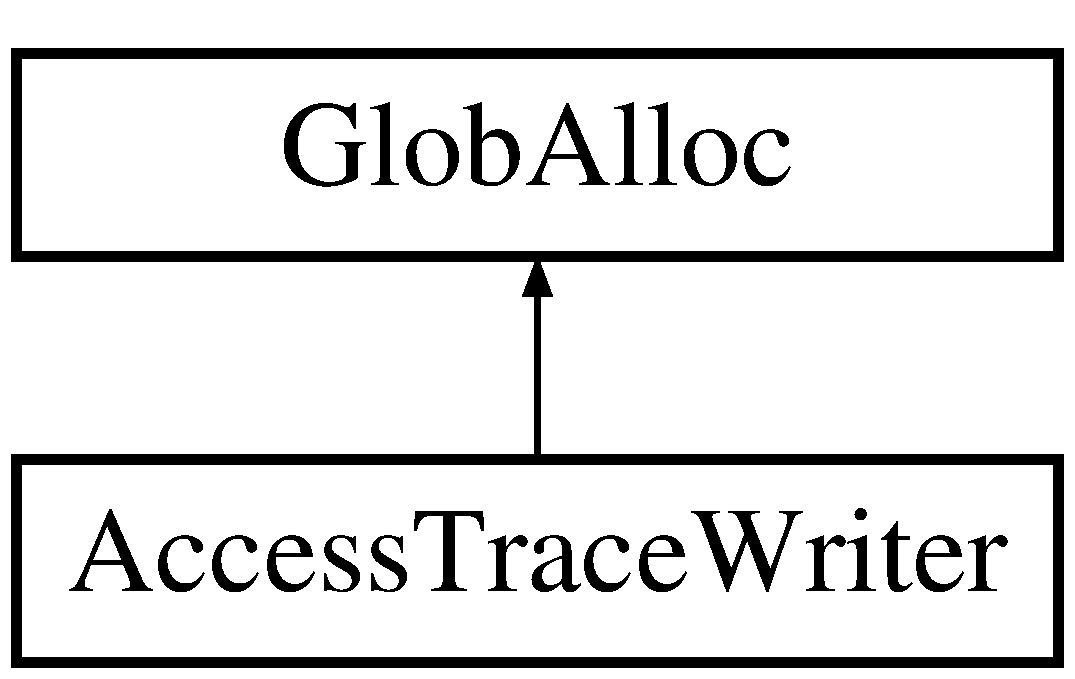
\includegraphics[height=2.000000cm]{classAccessTraceWriter}
\end{center}
\end{figure}
\subsection*{Public Member Functions}
\begin{DoxyCompactItemize}
\item 
\hypertarget{classAccessTraceWriter_a3568333a53ecf4ec44662e0672f8be82}{{\bfseries Access\-Trace\-Writer} (g\-\_\-string fname, uint32\-\_\-t num\-Children)}\label{classAccessTraceWriter_a3568333a53ecf4ec44662e0672f8be82}

\item 
\hypertarget{classAccessTraceWriter_a969899467ba61480b908533ca4c5b8e9}{void {\bfseries write} (\hyperlink{structAccessRecord}{Access\-Record} \&acc)}\label{classAccessTraceWriter_a969899467ba61480b908533ca4c5b8e9}

\item 
\hypertarget{classAccessTraceWriter_a8cfa74417b866f32240f174df5ce6805}{void {\bfseries dump} (bool cont)}\label{classAccessTraceWriter_a8cfa74417b866f32240f174df5ce6805}

\end{DoxyCompactItemize}


The documentation for this class was generated from the following files\-:\begin{DoxyCompactItemize}
\item 
access\-\_\-tracing.\-h\item 
access\-\_\-tracing.\-cpp\end{DoxyCompactItemize}

\hypertarget{classActWindow}{\section{Act\-Window Class Reference}
\label{classActWindow}\index{Act\-Window@{Act\-Window}}
}


{\ttfamily \#include $<$ddr\-\_\-mem.\-h$>$}

\subsection*{Public Member Functions}
\begin{DoxyCompactItemize}
\item 
\hypertarget{classActWindow_a225548b760e388e0b6973c1186b341cc}{void {\bfseries init} (uint32\-\_\-t size)}\label{classActWindow_a225548b760e388e0b6973c1186b341cc}

\item 
\hypertarget{classActWindow_a3727d383d4d5a32afdf1f12ba9674a0a}{uint64\-\_\-t {\bfseries min\-Act\-Cycle} () const }\label{classActWindow_a3727d383d4d5a32afdf1f12ba9674a0a}

\item 
\hypertarget{classActWindow_a062fcd84cef712aa8c05cc7078d3ed06}{void {\bfseries add\-Activation} (uint64\-\_\-t act\-Cycle)}\label{classActWindow_a062fcd84cef712aa8c05cc7078d3ed06}

\end{DoxyCompactItemize}


\subsection{Detailed Description}
\$lic\$ Copyright (C) 2012-\/2015 by Massachusetts Institute of Technology Copyright (C) 2010-\/2013 by The Board of Trustees of Stanford University

This file is part of zsim.

zsim is free software; you can redistribute it and/or modify it under the terms of the G\-N\-U General Public License as published by the Free Software Foundation, version 2.

If you use this software in your research, we request that you reference the zsim paper (\char`\"{}\-Z\-Sim\-: Fast and Accurate Microarchitectural Simulation of
\-Thousand-\/\-Core Systems\char`\"{}, Sanchez and Kozyrakis, I\-S\-C\-A-\/40, June 2013) as the source of the simulator in any publications that use this software, and that you send us a citation of your work.

zsim is distributed in the hope that it will be useful, but W\-I\-T\-H\-O\-U\-T A\-N\-Y W\-A\-R\-R\-A\-N\-T\-Y; without even the implied warranty of M\-E\-R\-C\-H\-A\-N\-T\-A\-B\-I\-L\-I\-T\-Y or F\-I\-T\-N\-E\-S\-S F\-O\-R A P\-A\-R\-T\-I\-C\-U\-L\-A\-R P\-U\-R\-P\-O\-S\-E. See the G\-N\-U General Public License for more details.

You should have received a copy of the G\-N\-U General Public License along with this program. If not, see \href{http://www.gnu.org/licenses/}{\tt http\-://www.\-gnu.\-org/licenses/}. 

The documentation for this class was generated from the following file\-:\begin{DoxyCompactItemize}
\item 
ddr\-\_\-mem.\-h\end{DoxyCompactItemize}

\hypertarget{classAdaptiveEvent}{\section{Adaptive\-Event$<$ G, F $>$ Class Template Reference}
\label{classAdaptiveEvent}\index{Adaptive\-Event$<$ G, F $>$@{Adaptive\-Event$<$ G, F $>$}}
}
Inheritance diagram for Adaptive\-Event$<$ G, F $>$\-:\begin{figure}[H]
\begin{center}
\leavevmode
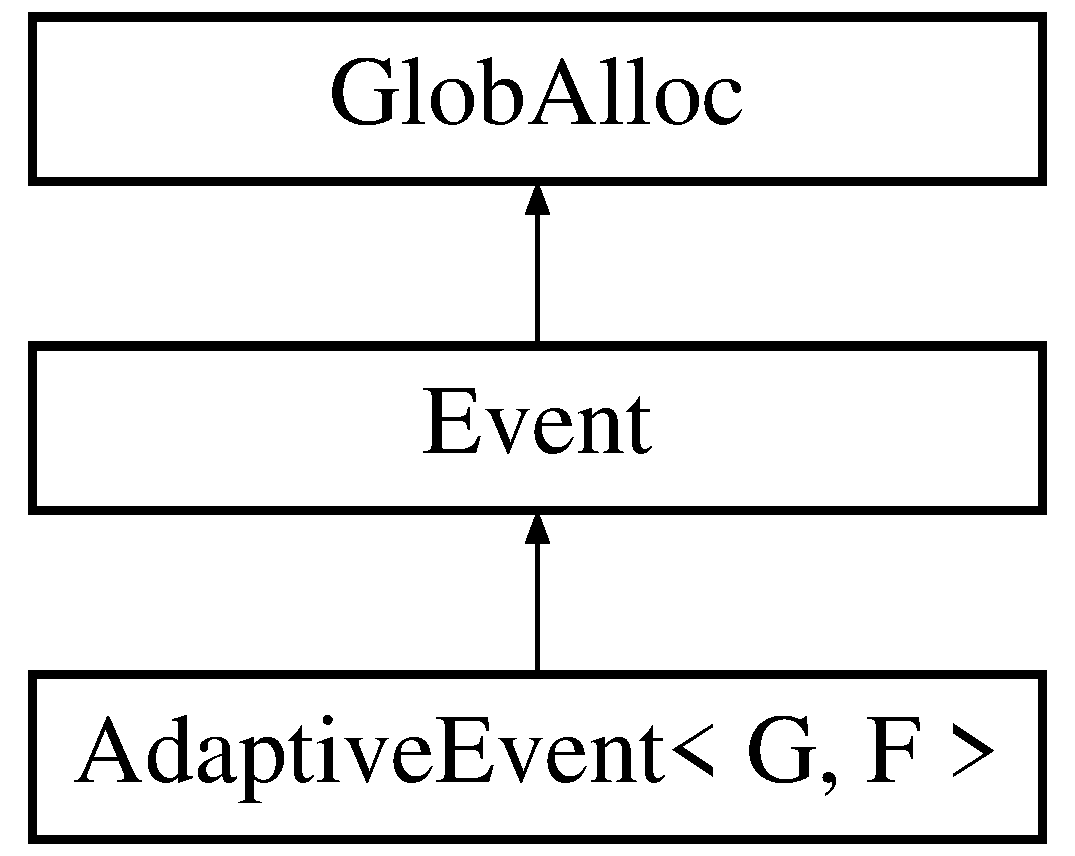
\includegraphics[height=3.000000cm]{classAdaptiveEvent}
\end{center}
\end{figure}
\subsection*{Public Member Functions}
\begin{DoxyCompactItemize}
\item 
\hypertarget{classAdaptiveEvent_a7b471bbf4cc9e8e64e7e7e361e5d7d82}{{\bfseries Adaptive\-Event} (G \-\_\-get, F \-\_\-fire, uint64\-\_\-t \-\_\-start, uint64\-\_\-t \-\_\-target, uint64\-\_\-t \-\_\-max\-Rate)}\label{classAdaptiveEvent_a7b471bbf4cc9e8e64e7e7e361e5d7d82}

\item 
\hypertarget{classAdaptiveEvent_ad59239ff5a5a2284754edc3cdb42514e}{void {\bfseries callback} ()}\label{classAdaptiveEvent_ad59239ff5a5a2284754edc3cdb42514e}

\end{DoxyCompactItemize}
\subsection*{Additional Inherited Members}


The documentation for this class was generated from the following file\-:\begin{DoxyCompactItemize}
\item 
event\-\_\-queue.\-h\end{DoxyCompactItemize}

\hypertarget{classAggregateStat}{\section{Aggregate\-Stat Class Reference}
\label{classAggregateStat}\index{Aggregate\-Stat@{Aggregate\-Stat}}
}
Inheritance diagram for Aggregate\-Stat\-:\begin{figure}[H]
\begin{center}
\leavevmode
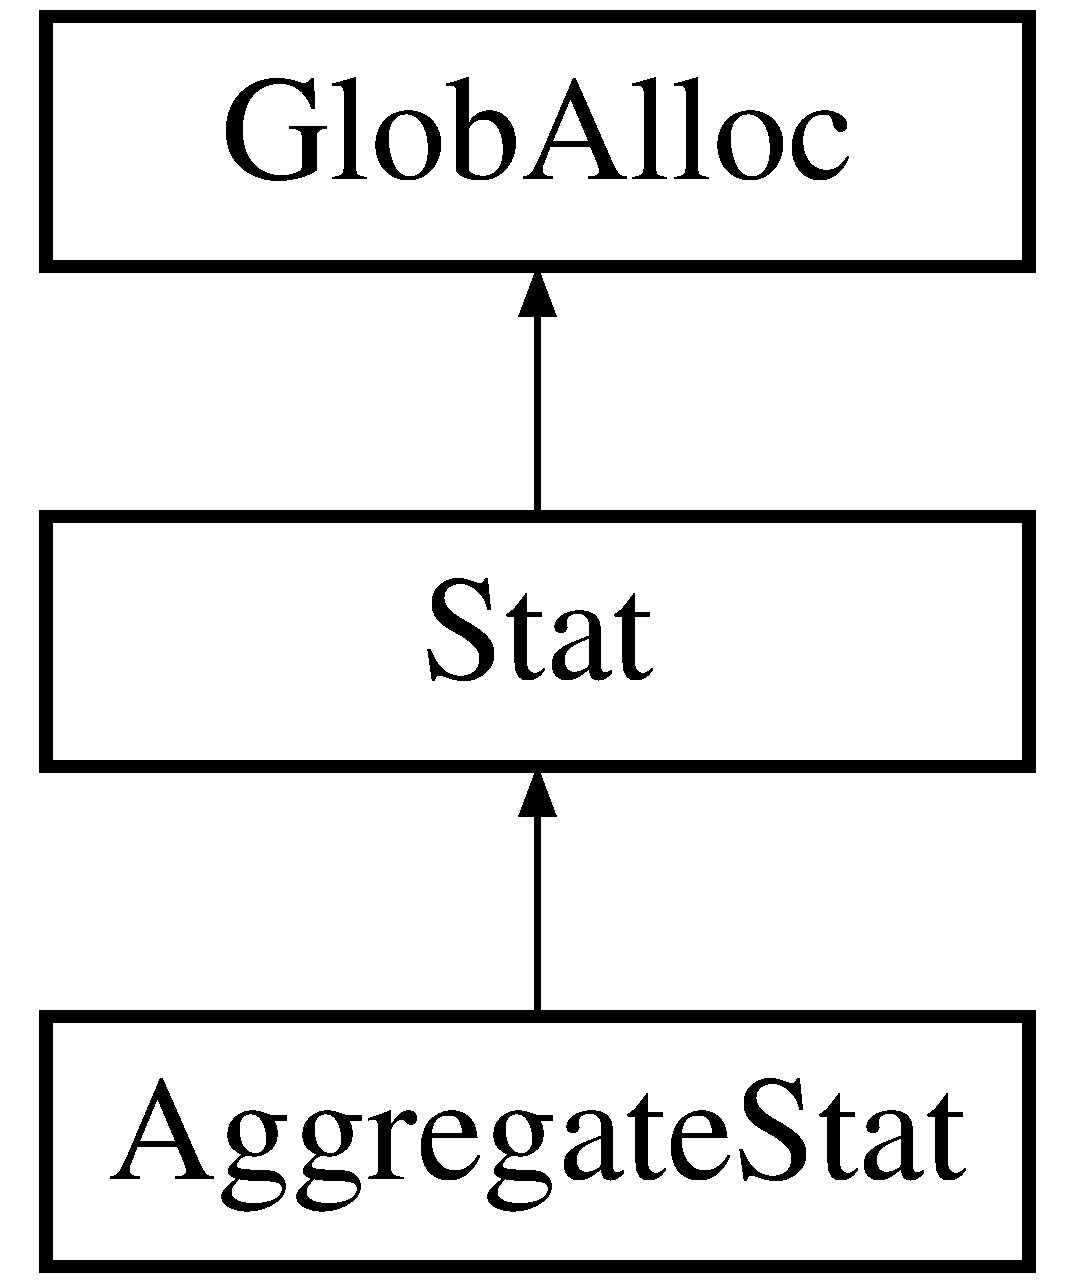
\includegraphics[height=3.000000cm]{classAggregateStat}
\end{center}
\end{figure}
\subsection*{Public Member Functions}
\begin{DoxyCompactItemize}
\item 
\hypertarget{classAggregateStat_a4f69488195511be076a792bd6b4bb4d3}{{\bfseries Aggregate\-Stat} (bool is\-Regular=false)}\label{classAggregateStat_a4f69488195511be076a792bd6b4bb4d3}

\item 
\hypertarget{classAggregateStat_a5a872e7b0af5362eaae6b304fef84238}{void {\bfseries init} (const char $\ast$name, const char $\ast$desc)}\label{classAggregateStat_a5a872e7b0af5362eaae6b304fef84238}

\item 
\hypertarget{classAggregateStat_ab2265e46065d4664f3f4507a8c3691b1}{bool {\bfseries make\-Immutable} ()}\label{classAggregateStat_ab2265e46065d4664f3f4507a8c3691b1}

\item 
\hypertarget{classAggregateStat_af4f3bbb6a336b481299b936ddcced4cb}{void {\bfseries append} (\hyperlink{classStat}{Stat} $\ast$child)}\label{classAggregateStat_af4f3bbb6a336b481299b936ddcced4cb}

\item 
\hypertarget{classAggregateStat_a20e9df9e5246b41edd111b5088118d8a}{uint32\-\_\-t {\bfseries size} () const }\label{classAggregateStat_a20e9df9e5246b41edd111b5088118d8a}

\item 
\hypertarget{classAggregateStat_a0ecf5b1c93991c7d5c5cc4fa2c07287c}{bool {\bfseries is\-Regular} () const }\label{classAggregateStat_a0ecf5b1c93991c7d5c5cc4fa2c07287c}

\item 
\hypertarget{classAggregateStat_a52c0cebe85e6e2f147329a3f3ad771a7}{\hyperlink{classStat}{Stat} $\ast$ {\bfseries get} (uint32\-\_\-t idx) const }\label{classAggregateStat_a52c0cebe85e6e2f147329a3f3ad771a7}

\item 
\hypertarget{classAggregateStat_a79cb6a42f80d59c331cba872eff8d6ff}{uint32\-\_\-t {\bfseries cur\-Size} () const }\label{classAggregateStat_a79cb6a42f80d59c331cba872eff8d6ff}

\end{DoxyCompactItemize}
\subsection*{Additional Inherited Members}


The documentation for this class was generated from the following file\-:\begin{DoxyCompactItemize}
\item 
stats.\-h\end{DoxyCompactItemize}

\hypertarget{classaligned__mutex}{\section{aligned\-\_\-mutex Class Reference}
\label{classaligned__mutex}\index{aligned\-\_\-mutex@{aligned\-\_\-mutex}}
}
Inheritance diagram for aligned\-\_\-mutex\-:\begin{figure}[H]
\begin{center}
\leavevmode
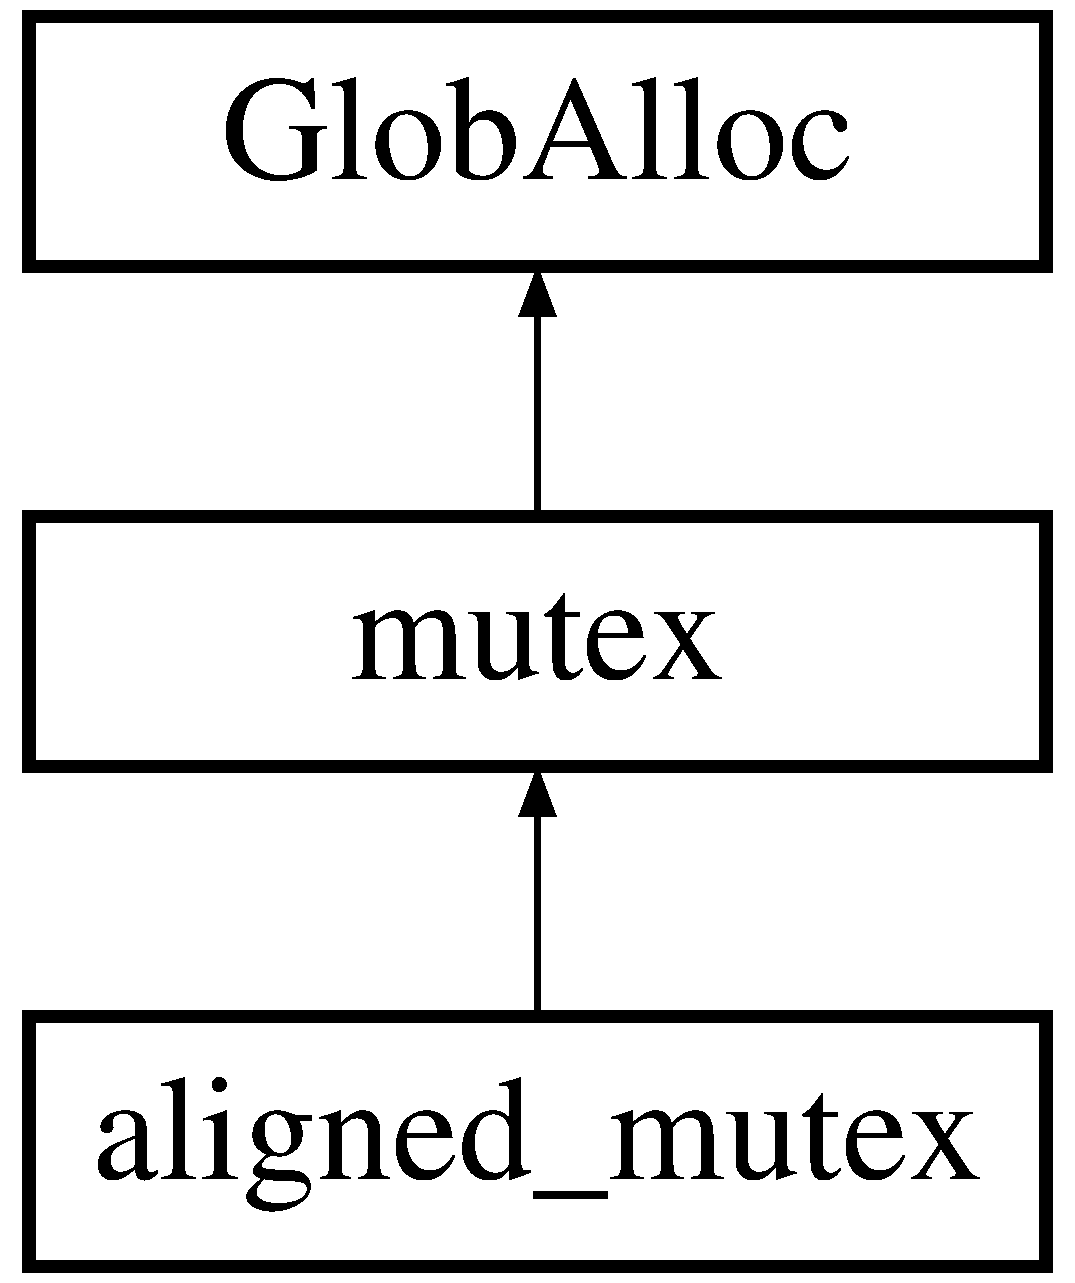
\includegraphics[height=3.000000cm]{classaligned__mutex}
\end{center}
\end{figure}
\subsection*{Additional Inherited Members}


The documentation for this class was generated from the following file\-:\begin{DoxyCompactItemize}
\item 
mutex.\-h\end{DoxyCompactItemize}

\hypertarget{classBarrier}{\section{Barrier Class Reference}
\label{classBarrier}\index{Barrier@{Barrier}}
}
Inheritance diagram for Barrier\-:\begin{figure}[H]
\begin{center}
\leavevmode
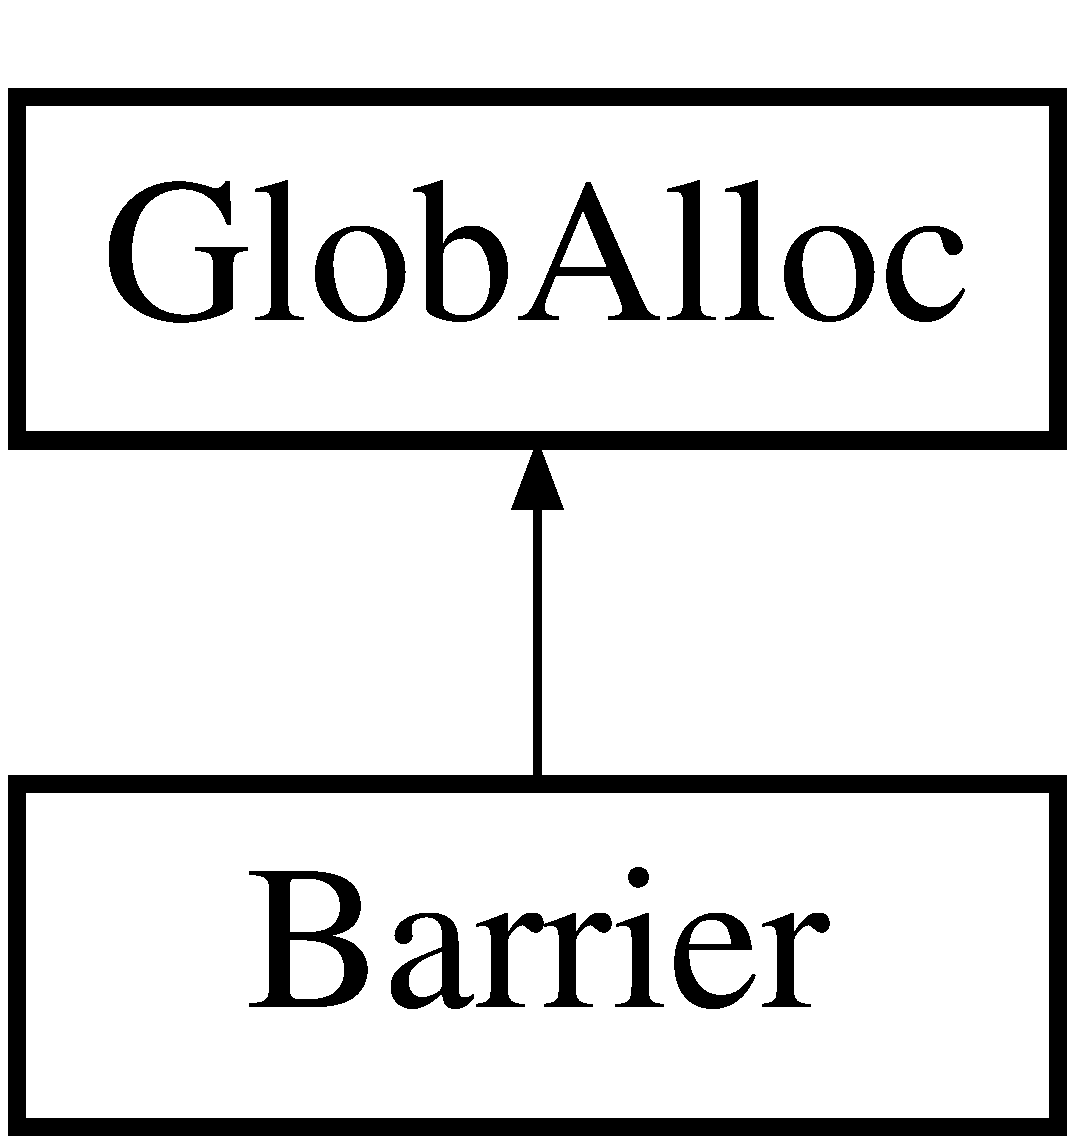
\includegraphics[height=2.000000cm]{classBarrier}
\end{center}
\end{figure}
\subsection*{Public Member Functions}
\begin{DoxyCompactItemize}
\item 
\hypertarget{classBarrier_afba5acbf7c4c59a188b7095427d6bca8}{{\bfseries Barrier} (uint32\-\_\-t \-\_\-parallel\-Threads, \hyperlink{classCallee}{Callee} $\ast$\-\_\-sched)}\label{classBarrier_afba5acbf7c4c59a188b7095427d6bca8}

\item 
\hypertarget{classBarrier_acf3161220f8103268e839886aa5abd7e}{void {\bfseries join} (uint32\-\_\-t tid, lock\-\_\-t $\ast$sched\-Lock)}\label{classBarrier_acf3161220f8103268e839886aa5abd7e}

\item 
\hypertarget{classBarrier_a9f8323ec211fee7ab01ecd5a09915b15}{void {\bfseries leave} (uint32\-\_\-t tid)}\label{classBarrier_a9f8323ec211fee7ab01ecd5a09915b15}

\item 
\hypertarget{classBarrier_ade91fab85fc326b8484e9aa0e24c33c7}{void {\bfseries sync} (uint32\-\_\-t tid, lock\-\_\-t $\ast$sched\-Lock)}\label{classBarrier_ade91fab85fc326b8484e9aa0e24c33c7}

\end{DoxyCompactItemize}


The documentation for this class was generated from the following file\-:\begin{DoxyCompactItemize}
\item 
barrier.\-h\end{DoxyCompactItemize}

\hypertarget{classBaseCache}{\section{Base\-Cache Class Reference}
\label{classBaseCache}\index{Base\-Cache@{Base\-Cache}}
}
Inheritance diagram for Base\-Cache\-:\begin{figure}[H]
\begin{center}
\leavevmode
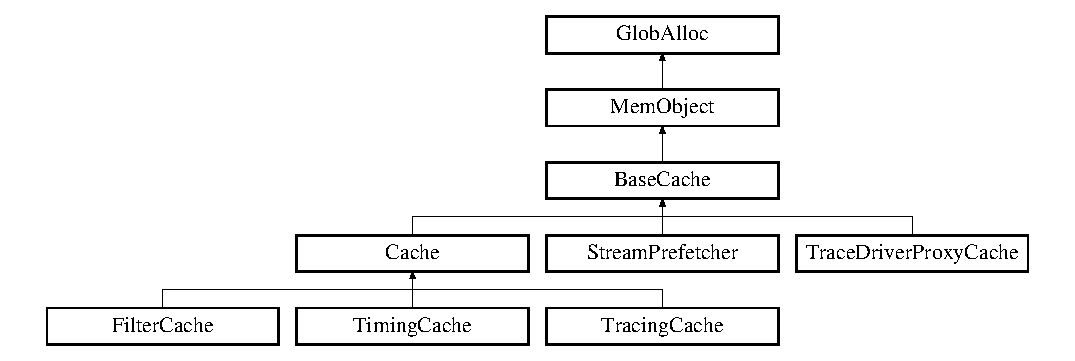
\includegraphics[height=4.402516cm]{classBaseCache}
\end{center}
\end{figure}
\subsection*{Public Member Functions}
\begin{DoxyCompactItemize}
\item 
\hypertarget{classBaseCache_a869ed0b4434d75697a46e77279a89c37}{virtual void {\bfseries set\-Parents} (uint32\-\_\-t \-\_\-child\-Id, const \hyperlink{classg__vector}{g\-\_\-vector}$<$ \hyperlink{classMemObject}{Mem\-Object} $\ast$ $>$ \&parents, \hyperlink{classNetwork}{Network} $\ast$network)=0}\label{classBaseCache_a869ed0b4434d75697a46e77279a89c37}

\item 
\hypertarget{classBaseCache_a05e2d3cfe83d549065360b21bdaabea3}{virtual void {\bfseries set\-Children} (const \hyperlink{classg__vector}{g\-\_\-vector}$<$ \hyperlink{classBaseCache}{Base\-Cache} $\ast$ $>$ \&children, \hyperlink{classNetwork}{Network} $\ast$network)=0}\label{classBaseCache_a05e2d3cfe83d549065360b21bdaabea3}

\item 
\hypertarget{classBaseCache_adee591deb418ec0b938c20cfc40d335c}{virtual uint64\-\_\-t {\bfseries invalidate} (const \hyperlink{structInvReq}{Inv\-Req} \&req)=0}\label{classBaseCache_adee591deb418ec0b938c20cfc40d335c}

\end{DoxyCompactItemize}


The documentation for this class was generated from the following file\-:\begin{DoxyCompactItemize}
\item 
memory\-\_\-hierarchy.\-h\end{DoxyCompactItemize}

\hypertarget{structBblInfo}{\section{Bbl\-Info Struct Reference}
\label{structBblInfo}\index{Bbl\-Info@{Bbl\-Info}}
}


{\ttfamily \#include $<$core.\-h$>$}

\subsection*{Public Attributes}
\begin{DoxyCompactItemize}
\item 
\hypertarget{structBblInfo_a26381f3642e0d5511b7173d734e0a88d}{uint32\-\_\-t {\bfseries instrs}}\label{structBblInfo_a26381f3642e0d5511b7173d734e0a88d}

\item 
\hypertarget{structBblInfo_ae13e66a8604c69c30d5510b417f49908}{uint32\-\_\-t {\bfseries bytes}}\label{structBblInfo_ae13e66a8604c69c30d5510b417f49908}

\item 
\hypertarget{structBblInfo_a933e2aa85267361ec08c2b4583a68dea}{\hyperlink{structDynBbl}{Dyn\-Bbl} {\bfseries ooo\-Bbl} \mbox{[}0\mbox{]}}\label{structBblInfo_a933e2aa85267361ec08c2b4583a68dea}

\end{DoxyCompactItemize}


\subsection{Detailed Description}
\$lic\$ Copyright (C) 2012-\/2015 by Massachusetts Institute of Technology Copyright (C) 2010-\/2013 by The Board of Trustees of Stanford University

This file is part of zsim.

zsim is free software; you can redistribute it and/or modify it under the terms of the G\-N\-U General Public License as published by the Free Software Foundation, version 2.

If you use this software in your research, we request that you reference the zsim paper (\char`\"{}\-Z\-Sim\-: Fast and Accurate Microarchitectural Simulation of
\-Thousand-\/\-Core Systems\char`\"{}, Sanchez and Kozyrakis, I\-S\-C\-A-\/40, June 2013) as the source of the simulator in any publications that use this software, and that you send us a citation of your work.

zsim is distributed in the hope that it will be useful, but W\-I\-T\-H\-O\-U\-T A\-N\-Y W\-A\-R\-R\-A\-N\-T\-Y; without even the implied warranty of M\-E\-R\-C\-H\-A\-N\-T\-A\-B\-I\-L\-I\-T\-Y or F\-I\-T\-N\-E\-S\-S F\-O\-R A P\-A\-R\-T\-I\-C\-U\-L\-A\-R P\-U\-R\-P\-O\-S\-E. See the G\-N\-U General Public License for more details.

You should have received a copy of the G\-N\-U General Public License along with this program. If not, see \href{http://www.gnu.org/licenses/}{\tt http\-://www.\-gnu.\-org/licenses/}. 

The documentation for this struct was generated from the following file\-:\begin{DoxyCompactItemize}
\item 
core.\-h\end{DoxyCompactItemize}

\hypertarget{classBranchPredictorPAg}{\section{Branch\-Predictor\-P\-Ag$<$ N\-B, H\-B, L\-B $>$ Class Template Reference}
\label{classBranchPredictorPAg}\index{Branch\-Predictor\-P\-Ag$<$ N\-B, H\-B, L\-B $>$@{Branch\-Predictor\-P\-Ag$<$ N\-B, H\-B, L\-B $>$}}
}
\subsection*{Public Member Functions}
\begin{DoxyCompactItemize}
\item 
\hypertarget{classBranchPredictorPAg_a23a118b8dfac700a90fa7893a86a8268}{bool {\bfseries predict} (Address branch\-Pc, bool taken)}\label{classBranchPredictorPAg_a23a118b8dfac700a90fa7893a86a8268}

\end{DoxyCompactItemize}


The documentation for this class was generated from the following file\-:\begin{DoxyCompactItemize}
\item 
ooo\-\_\-core.\-h\end{DoxyCompactItemize}

\hypertarget{classCache}{\section{Cache Class Reference}
\label{classCache}\index{Cache@{Cache}}
}
Inheritance diagram for Cache\-:\begin{figure}[H]
\begin{center}
\leavevmode
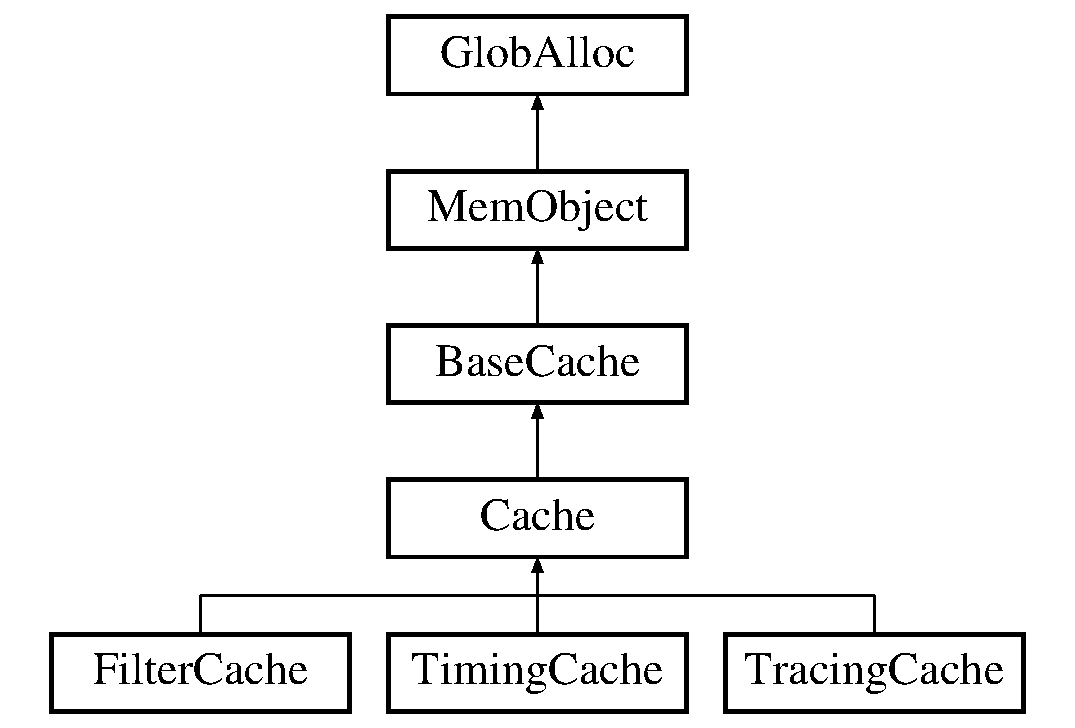
\includegraphics[height=5.000000cm]{classCache}
\end{center}
\end{figure}
\subsection*{Public Member Functions}
\begin{DoxyCompactItemize}
\item 
\hyperlink{classCache_a398112ee381973ef3777746a31900320}{Cache} (uint32\-\_\-t \-\_\-num\-Lines, \hyperlink{classCC}{C\-C} $\ast$\-\_\-cc, \hyperlink{classCacheArray}{Cache\-Array} $\ast$\-\_\-array, \hyperlink{classReplPolicy}{Repl\-Policy} $\ast$\-\_\-rp, uint32\-\_\-t \-\_\-acc\-Lat, uint32\-\_\-t \-\_\-inv\-Lat, const g\-\_\-string \&\-\_\-name)
\item 
\hypertarget{classCache_a723ba68ec1f3e8d46b536e003d2d31d4}{const char $\ast$ {\bfseries get\-Name} ()}\label{classCache_a723ba68ec1f3e8d46b536e003d2d31d4}

\item 
\hypertarget{classCache_a79ba01ab96d6949c8cf3f71cf310d9bd}{void {\bfseries set\-Parents} (uint32\-\_\-t \-\_\-child\-Id, const \hyperlink{classg__vector}{g\-\_\-vector}$<$ \hyperlink{classMemObject}{Mem\-Object} $\ast$ $>$ \&parents, \hyperlink{classNetwork}{Network} $\ast$network)}\label{classCache_a79ba01ab96d6949c8cf3f71cf310d9bd}

\item 
\hypertarget{classCache_a5c6c05094ed04256fd6f77a3ca20673e}{void {\bfseries set\-Children} (const \hyperlink{classg__vector}{g\-\_\-vector}$<$ \hyperlink{classBaseCache}{Base\-Cache} $\ast$ $>$ \&children, \hyperlink{classNetwork}{Network} $\ast$network)}\label{classCache_a5c6c05094ed04256fd6f77a3ca20673e}

\item 
\hypertarget{classCache_a3cd51a37ecac027028c662279fed96e3}{void {\bfseries init\-Stats} (\hyperlink{classAggregateStat}{Aggregate\-Stat} $\ast$parent\-Stat)}\label{classCache_a3cd51a37ecac027028c662279fed96e3}

\item 
\hypertarget{classCache_a7d23c3978dca10511edbfba724489a14}{virtual uint64\-\_\-t {\bfseries access} (\hyperlink{structMemReq}{Mem\-Req} \&req)}\label{classCache_a7d23c3978dca10511edbfba724489a14}

\item 
\hypertarget{classCache_a2b21fdc8a63f1c1a60b84643debe82db}{virtual uint64\-\_\-t {\bfseries invalidate} (const \hyperlink{structInvReq}{Inv\-Req} \&req)}\label{classCache_a2b21fdc8a63f1c1a60b84643debe82db}

\end{DoxyCompactItemize}
\subsection*{Protected Member Functions}
\begin{DoxyCompactItemize}
\item 
\hypertarget{classCache_a6f04561d53efc7623c809e6c885d8c09}{void {\bfseries init\-Cache\-Stats} (\hyperlink{classAggregateStat}{Aggregate\-Stat} $\ast$cache\-Stat)}\label{classCache_a6f04561d53efc7623c809e6c885d8c09}

\item 
\hypertarget{classCache_acd207b095f2b950d8887a1f9614f994b}{void {\bfseries start\-Invalidate} ()}\label{classCache_acd207b095f2b950d8887a1f9614f994b}

\item 
\hypertarget{classCache_abde65d6c87557ccdf3557e6da05dcb7c}{uint64\-\_\-t {\bfseries finish\-Invalidate} (const \hyperlink{structInvReq}{Inv\-Req} \&req)}\label{classCache_abde65d6c87557ccdf3557e6da05dcb7c}

\end{DoxyCompactItemize}
\subsection*{Protected Attributes}
\begin{DoxyCompactItemize}
\item 
\hypertarget{classCache_a279fee4d6cedcfb14394e6971be01978}{\hyperlink{classCC}{C\-C} $\ast$ {\bfseries cc}}\label{classCache_a279fee4d6cedcfb14394e6971be01978}

\item 
\hypertarget{classCache_a2af76891495aab963a368ffd9ccde010}{\hyperlink{classCacheArray}{Cache\-Array} $\ast$ {\bfseries array}}\label{classCache_a2af76891495aab963a368ffd9ccde010}

\item 
\hypertarget{classCache_a93822b507943d4a2383ad83e1d706582}{\hyperlink{classReplPolicy}{Repl\-Policy} $\ast$ {\bfseries rp}}\label{classCache_a93822b507943d4a2383ad83e1d706582}

\item 
\hypertarget{classCache_a0d43aadafe65c0753c8656f315e27a8d}{uint32\-\_\-t {\bfseries num\-Lines}}\label{classCache_a0d43aadafe65c0753c8656f315e27a8d}

\item 
\hypertarget{classCache_acec1448a346c8ebf5412d4ba0d8f0645}{uint32\-\_\-t {\bfseries acc\-Lat}}\label{classCache_acec1448a346c8ebf5412d4ba0d8f0645}

\item 
\hypertarget{classCache_adeafa997d10220f79e5cf85c1c3ab46e}{uint32\-\_\-t {\bfseries inv\-Lat}}\label{classCache_adeafa997d10220f79e5cf85c1c3ab46e}

\item 
\hypertarget{classCache_a85342a02c0ac63167a48b6792e13e8d9}{g\-\_\-string {\bfseries name}}\label{classCache_a85342a02c0ac63167a48b6792e13e8d9}

\end{DoxyCompactItemize}


\subsection{Constructor \& Destructor Documentation}
\hypertarget{classCache_a398112ee381973ef3777746a31900320}{\index{Cache@{Cache}!Cache@{Cache}}
\index{Cache@{Cache}!Cache@{Cache}}
\subsubsection[{Cache}]{\setlength{\rightskip}{0pt plus 5cm}Cache\-::\-Cache (
\begin{DoxyParamCaption}
\item[{uint32\-\_\-t}]{\-\_\-num\-Lines, }
\item[{{\bf C\-C} $\ast$}]{\-\_\-cc, }
\item[{{\bf Cache\-Array} $\ast$}]{\-\_\-array, }
\item[{{\bf Repl\-Policy} $\ast$}]{\-\_\-rp, }
\item[{uint32\-\_\-t}]{\-\_\-acc\-Lat, }
\item[{uint32\-\_\-t}]{\-\_\-inv\-Lat, }
\item[{const g\-\_\-string \&}]{\-\_\-name}
\end{DoxyParamCaption}
)}}\label{classCache_a398112ee381973ef3777746a31900320}
\$lic\$ Copyright (C) 2012-\/2015 by Massachusetts Institute of Technology Copyright (C) 2010-\/2013 by The Board of Trustees of Stanford University

This file is part of zsim.

zsim is free software; you can redistribute it and/or modify it under the terms of the G\-N\-U General Public License as published by the Free Software Foundation, version 2.

If you use this software in your research, we request that you reference the zsim paper (\char`\"{}\-Z\-Sim\-: Fast and Accurate Microarchitectural Simulation of
\-Thousand-\/\-Core Systems\char`\"{}, Sanchez and Kozyrakis, I\-S\-C\-A-\/40, June 2013) as the source of the simulator in any publications that use this software, and that you send us a citation of your work.

zsim is distributed in the hope that it will be useful, but W\-I\-T\-H\-O\-U\-T A\-N\-Y W\-A\-R\-R\-A\-N\-T\-Y; without even the implied warranty of M\-E\-R\-C\-H\-A\-N\-T\-A\-B\-I\-L\-I\-T\-Y or F\-I\-T\-N\-E\-S\-S F\-O\-R A P\-A\-R\-T\-I\-C\-U\-L\-A\-R P\-U\-R\-P\-O\-S\-E. See the G\-N\-U General Public License for more details.

You should have received a copy of the G\-N\-U General Public License along with this program. If not, see \href{http://www.gnu.org/licenses/}{\tt http\-://www.\-gnu.\-org/licenses/}. 

The documentation for this class was generated from the following files\-:\begin{DoxyCompactItemize}
\item 
cache.\-h\item 
cache.\-cpp\end{DoxyCompactItemize}

\hypertarget{classCacheArray}{\section{Cache\-Array Class Reference}
\label{classCacheArray}\index{Cache\-Array@{Cache\-Array}}
}


{\ttfamily \#include $<$cache\-\_\-arrays.\-h$>$}

Inheritance diagram for Cache\-Array\-:\begin{figure}[H]
\begin{center}
\leavevmode
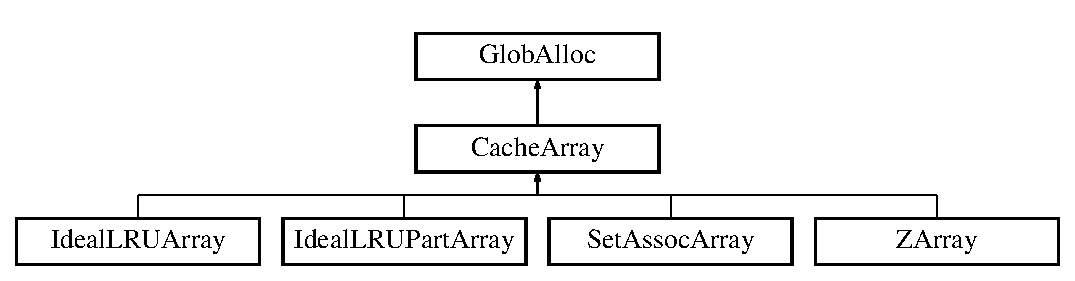
\includegraphics[height=3.000000cm]{classCacheArray}
\end{center}
\end{figure}
\subsection*{Public Member Functions}
\begin{DoxyCompactItemize}
\item 
\hypertarget{classCacheArray_a2c638cb1d7a7899dd00a22b07327f598}{virtual int32\-\_\-t {\bfseries lookup} (const Address line\-Addr, const \hyperlink{structMemReq}{Mem\-Req} $\ast$req, bool update\-Replacement)=0}\label{classCacheArray_a2c638cb1d7a7899dd00a22b07327f598}

\item 
\hypertarget{classCacheArray_acf1528a7fbf12c7cc339353372ab8f2e}{virtual uint32\-\_\-t {\bfseries preinsert} (const Address line\-Addr, const \hyperlink{structMemReq}{Mem\-Req} $\ast$req, Address $\ast$wb\-Line\-Addr)=0}\label{classCacheArray_acf1528a7fbf12c7cc339353372ab8f2e}

\item 
\hypertarget{classCacheArray_ace44aa583ab1e84f9fe778d8b6ad8ce2}{virtual void {\bfseries postinsert} (const Address line\-Addr, const \hyperlink{structMemReq}{Mem\-Req} $\ast$req, uint32\-\_\-t line\-Id)=0}\label{classCacheArray_ace44aa583ab1e84f9fe778d8b6ad8ce2}

\item 
\hypertarget{classCacheArray_aca28881799337dc402d29d491e24efdb}{virtual void {\bfseries init\-Stats} (\hyperlink{classAggregateStat}{Aggregate\-Stat} $\ast$parent)}\label{classCacheArray_aca28881799337dc402d29d491e24efdb}

\end{DoxyCompactItemize}


\subsection{Detailed Description}
\$lic\$ Copyright (C) 2012-\/2015 by Massachusetts Institute of Technology Copyright (C) 2010-\/2013 by The Board of Trustees of Stanford University

This file is part of zsim.

zsim is free software; you can redistribute it and/or modify it under the terms of the G\-N\-U General Public License as published by the Free Software Foundation, version 2.

If you use this software in your research, we request that you reference the zsim paper (\char`\"{}\-Z\-Sim\-: Fast and Accurate Microarchitectural Simulation of
\-Thousand-\/\-Core Systems\char`\"{}, Sanchez and Kozyrakis, I\-S\-C\-A-\/40, June 2013) as the source of the simulator in any publications that use this software, and that you send us a citation of your work.

zsim is distributed in the hope that it will be useful, but W\-I\-T\-H\-O\-U\-T A\-N\-Y W\-A\-R\-R\-A\-N\-T\-Y; without even the implied warranty of M\-E\-R\-C\-H\-A\-N\-T\-A\-B\-I\-L\-I\-T\-Y or F\-I\-T\-N\-E\-S\-S F\-O\-R A P\-A\-R\-T\-I\-C\-U\-L\-A\-R P\-U\-R\-P\-O\-S\-E. See the G\-N\-U General Public License for more details.

You should have received a copy of the G\-N\-U General Public License along with this program. If not, see \href{http://www.gnu.org/licenses/}{\tt http\-://www.\-gnu.\-org/licenses/}. 

The documentation for this class was generated from the following file\-:\begin{DoxyCompactItemize}
\item 
cache\-\_\-arrays.\-h\end{DoxyCompactItemize}

\hypertarget{classDRAMSim_1_1Callback}{\section{D\-R\-A\-M\-Sim\-:\-:Callback$<$ Consumer\-T, Return\-T, Param1\-T, Param2\-T, Param3\-T $>$ Class Template Reference}
\label{classDRAMSim_1_1Callback}\index{D\-R\-A\-M\-Sim\-::\-Callback$<$ Consumer\-T, Return\-T, Param1\-T, Param2\-T, Param3\-T $>$@{D\-R\-A\-M\-Sim\-::\-Callback$<$ Consumer\-T, Return\-T, Param1\-T, Param2\-T, Param3\-T $>$}}
}
Inheritance diagram for D\-R\-A\-M\-Sim\-:\-:Callback$<$ Consumer\-T, Return\-T, Param1\-T, Param2\-T, Param3\-T $>$\-:\begin{figure}[H]
\begin{center}
\leavevmode
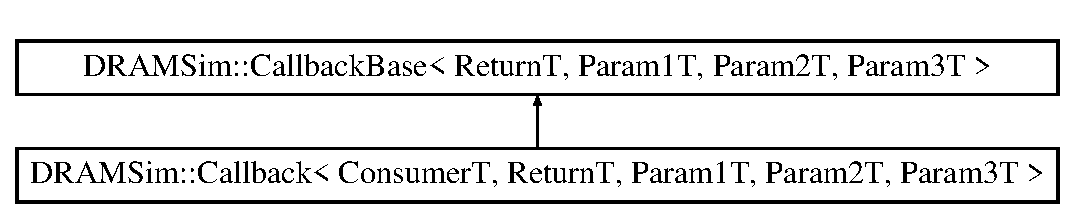
\includegraphics[height=2.000000cm]{classDRAMSim_1_1Callback}
\end{center}
\end{figure}
\subsection*{Public Member Functions}
\begin{DoxyCompactItemize}
\item 
\hypertarget{classDRAMSim_1_1Callback_a9218078cc5213b32f2bdbd8f2b32156d}{{\bfseries Callback} (Consumer\-T $\ast$const object, Ptr\-Member member)}\label{classDRAMSim_1_1Callback_a9218078cc5213b32f2bdbd8f2b32156d}

\item 
\hypertarget{classDRAMSim_1_1Callback_a73b50bc52f1aa9bc3881904d53e27638}{{\bfseries Callback} (const \hyperlink{classDRAMSim_1_1Callback}{Callback}$<$ Consumer\-T, Return\-T, Param1\-T, Param2\-T, Param3\-T $>$ \&e)}\label{classDRAMSim_1_1Callback_a73b50bc52f1aa9bc3881904d53e27638}

\item 
\hypertarget{classDRAMSim_1_1Callback_a43d30eea69ef321345952a92fbfc6108}{Return\-T {\bfseries operator()} (Param1\-T param1, Param2\-T param2, Param3\-T param3)}\label{classDRAMSim_1_1Callback_a43d30eea69ef321345952a92fbfc6108}

\end{DoxyCompactItemize}


The documentation for this class was generated from the following file\-:\begin{DoxyCompactItemize}
\item 
Callback.\-h\end{DoxyCompactItemize}

\hypertarget{classDRAMSim_1_1CallbackBase}{\section{D\-R\-A\-M\-Sim\-:\-:Callback\-Base$<$ Return\-T, Param1\-T, Param2\-T, Param3\-T $>$ Class Template Reference}
\label{classDRAMSim_1_1CallbackBase}\index{D\-R\-A\-M\-Sim\-::\-Callback\-Base$<$ Return\-T, Param1\-T, Param2\-T, Param3\-T $>$@{D\-R\-A\-M\-Sim\-::\-Callback\-Base$<$ Return\-T, Param1\-T, Param2\-T, Param3\-T $>$}}
}
Inheritance diagram for D\-R\-A\-M\-Sim\-:\-:Callback\-Base$<$ Return\-T, Param1\-T, Param2\-T, Param3\-T $>$\-:\begin{figure}[H]
\begin{center}
\leavevmode
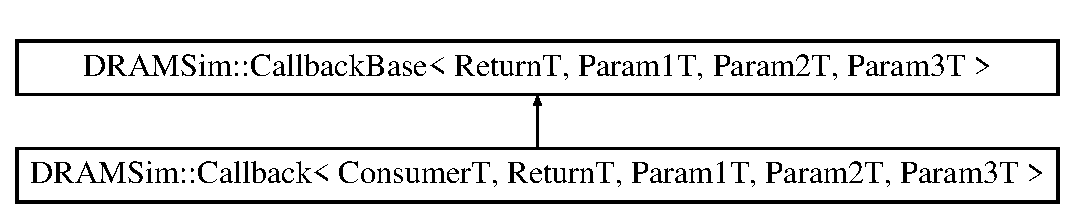
\includegraphics[height=2.000000cm]{classDRAMSim_1_1CallbackBase}
\end{center}
\end{figure}
\subsection*{Public Member Functions}
\begin{DoxyCompactItemize}
\item 
\hypertarget{classDRAMSim_1_1CallbackBase_abe02615a53f1dd67dfc26ca011c7e1a8}{virtual Return\-T {\bfseries operator()} (Param1\-T, Param2\-T, Param3\-T)=0}\label{classDRAMSim_1_1CallbackBase_abe02615a53f1dd67dfc26ca011c7e1a8}

\end{DoxyCompactItemize}


The documentation for this class was generated from the following file\-:\begin{DoxyCompactItemize}
\item 
Callback.\-h\end{DoxyCompactItemize}

\hypertarget{classCallee}{\section{Callee Class Reference}
\label{classCallee}\index{Callee@{Callee}}
}
Inheritance diagram for Callee\-:\begin{figure}[H]
\begin{center}
\leavevmode
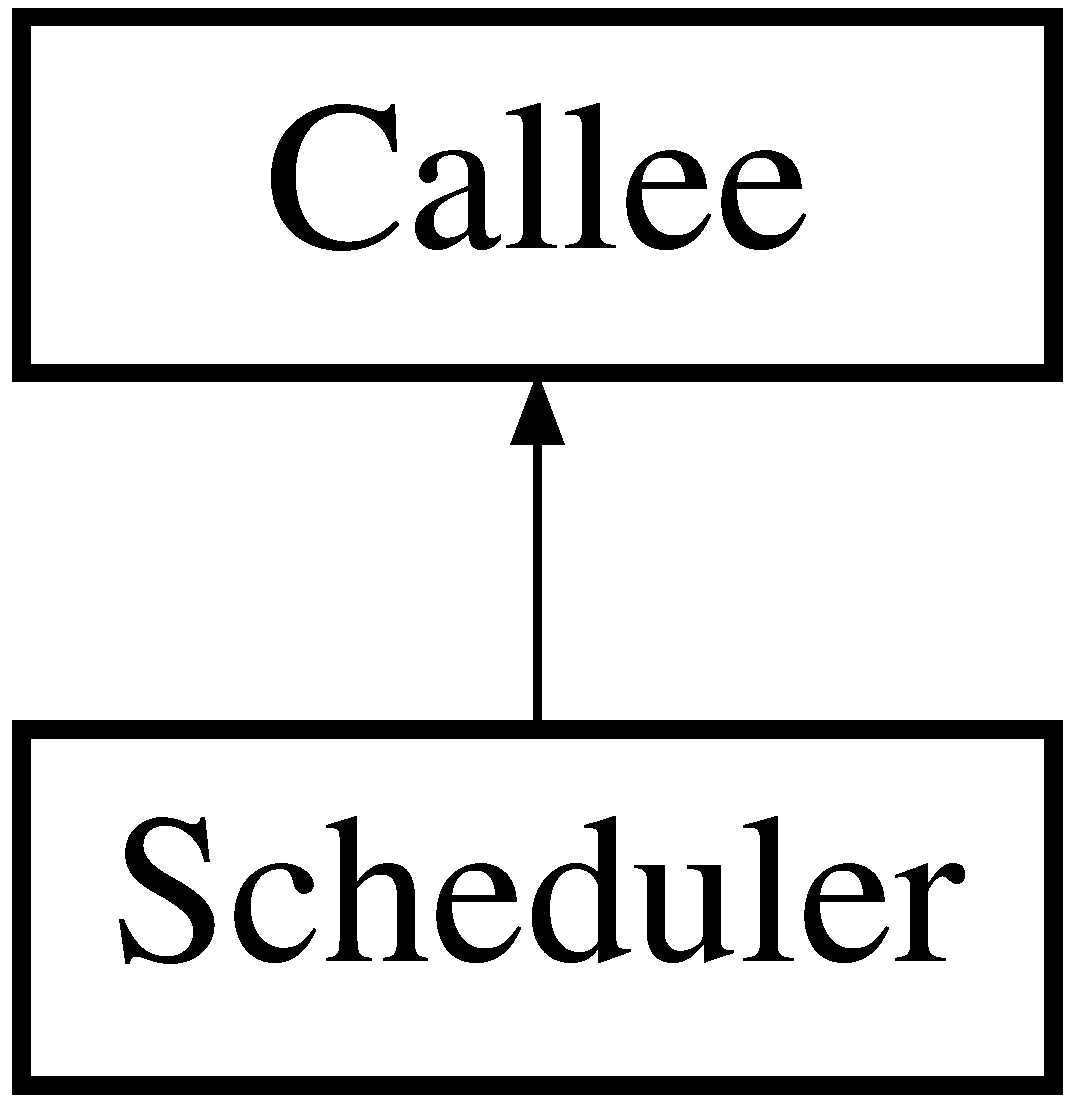
\includegraphics[height=2.000000cm]{classCallee}
\end{center}
\end{figure}
\subsection*{Public Member Functions}
\begin{DoxyCompactItemize}
\item 
\hypertarget{classCallee_a9224b75c8810dcdd2b8eefec4767d151}{virtual void {\bfseries callback} ()=0}\label{classCallee_a9224b75c8810dcdd2b8eefec4767d151}

\end{DoxyCompactItemize}


The documentation for this class was generated from the following file\-:\begin{DoxyCompactItemize}
\item 
barrier.\-h\end{DoxyCompactItemize}

\hypertarget{classCC}{\section{C\-C Class Reference}
\label{classCC}\index{C\-C@{C\-C}}
}


{\ttfamily \#include $<$coherence\-\_\-ctrls.\-h$>$}

Inheritance diagram for C\-C\-:\begin{figure}[H]
\begin{center}
\leavevmode
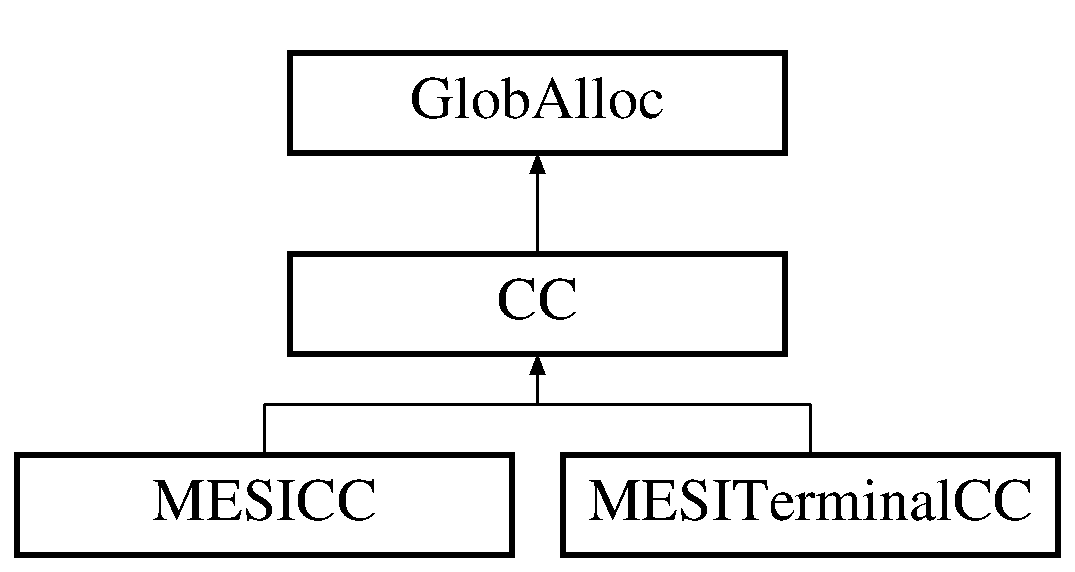
\includegraphics[height=3.000000cm]{classCC}
\end{center}
\end{figure}
\subsection*{Public Member Functions}
\begin{DoxyCompactItemize}
\item 
\hypertarget{classCC_a6b9d8a6acc32a2c279601078105ba94a}{virtual void {\bfseries set\-Parents} (uint32\-\_\-t child\-Id, const \hyperlink{classg__vector}{g\-\_\-vector}$<$ \hyperlink{classMemObject}{Mem\-Object} $\ast$ $>$ \&parents, \hyperlink{classNetwork}{Network} $\ast$network)=0}\label{classCC_a6b9d8a6acc32a2c279601078105ba94a}

\item 
\hypertarget{classCC_adcf73db25d1a7f19d875702cbd7d8da9}{virtual void {\bfseries set\-Children} (const \hyperlink{classg__vector}{g\-\_\-vector}$<$ \hyperlink{classBaseCache}{Base\-Cache} $\ast$ $>$ \&children, \hyperlink{classNetwork}{Network} $\ast$network)=0}\label{classCC_adcf73db25d1a7f19d875702cbd7d8da9}

\item 
\hypertarget{classCC_ad7b4e368967adaaab4fa63d5959ddbfe}{virtual void {\bfseries init\-Stats} (\hyperlink{classAggregateStat}{Aggregate\-Stat} $\ast$cache\-Stat)=0}\label{classCC_ad7b4e368967adaaab4fa63d5959ddbfe}

\item 
\hypertarget{classCC_a9637d8220e3588e4b7fd0460b1d2475a}{virtual bool {\bfseries start\-Access} (\hyperlink{structMemReq}{Mem\-Req} \&req)=0}\label{classCC_a9637d8220e3588e4b7fd0460b1d2475a}

\item 
\hypertarget{classCC_acca766f3f8379cf6c17c0fca4b8d3739}{virtual bool {\bfseries should\-Allocate} (const \hyperlink{structMemReq}{Mem\-Req} \&req)=0}\label{classCC_acca766f3f8379cf6c17c0fca4b8d3739}

\item 
\hypertarget{classCC_a336af65349d49287492ddcaa6197c6b0}{virtual uint64\-\_\-t {\bfseries process\-Eviction} (const \hyperlink{structMemReq}{Mem\-Req} \&trigger\-Req, Address wb\-Line\-Addr, int32\-\_\-t line\-Id, uint64\-\_\-t start\-Cycle)=0}\label{classCC_a336af65349d49287492ddcaa6197c6b0}

\item 
\hypertarget{classCC_a193b1f060826af44506030c2a78cebde}{virtual uint64\-\_\-t {\bfseries process\-Access} (const \hyperlink{structMemReq}{Mem\-Req} \&req, int32\-\_\-t line\-Id, uint64\-\_\-t start\-Cycle, uint64\-\_\-t $\ast$get\-Done\-Cycle=nullptr)=0}\label{classCC_a193b1f060826af44506030c2a78cebde}

\item 
\hypertarget{classCC_a66848e057fd8894a77a28e797dbc155c}{virtual void {\bfseries end\-Access} (const \hyperlink{structMemReq}{Mem\-Req} \&req)=0}\label{classCC_a66848e057fd8894a77a28e797dbc155c}

\item 
\hypertarget{classCC_ac2219b6d1f3fea343d37c80cee92b93a}{virtual void {\bfseries start\-Inv} ()=0}\label{classCC_ac2219b6d1f3fea343d37c80cee92b93a}

\item 
\hypertarget{classCC_aa3689bb729527bf2ced5a7020f9fdf65}{virtual uint64\-\_\-t {\bfseries process\-Inv} (const \hyperlink{structInvReq}{Inv\-Req} \&req, int32\-\_\-t line\-Id, uint64\-\_\-t start\-Cycle)=0}\label{classCC_aa3689bb729527bf2ced5a7020f9fdf65}

\item 
\hypertarget{classCC_a369786ed281101d04db2d841b21fd58f}{virtual uint32\-\_\-t {\bfseries num\-Sharers} (uint32\-\_\-t line\-Id)=0}\label{classCC_a369786ed281101d04db2d841b21fd58f}

\item 
\hypertarget{classCC_ad27aac34c05038196e4b59ce97e63a71}{virtual bool {\bfseries is\-Valid} (uint32\-\_\-t line\-Id)=0}\label{classCC_ad27aac34c05038196e4b59ce97e63a71}

\end{DoxyCompactItemize}


\subsection{Detailed Description}
\$lic\$ Copyright (C) 2012-\/2015 by Massachusetts Institute of Technology Copyright (C) 2010-\/2013 by The Board of Trustees of Stanford University

This file is part of zsim.

zsim is free software; you can redistribute it and/or modify it under the terms of the G\-N\-U General Public License as published by the Free Software Foundation, version 2.

If you use this software in your research, we request that you reference the zsim paper (\char`\"{}\-Z\-Sim\-: Fast and Accurate Microarchitectural Simulation of
\-Thousand-\/\-Core Systems\char`\"{}, Sanchez and Kozyrakis, I\-S\-C\-A-\/40, June 2013) as the source of the simulator in any publications that use this software, and that you send us a citation of your work.

zsim is distributed in the hope that it will be useful, but W\-I\-T\-H\-O\-U\-T A\-N\-Y W\-A\-R\-R\-A\-N\-T\-Y; without even the implied warranty of M\-E\-R\-C\-H\-A\-N\-T\-A\-B\-I\-L\-I\-T\-Y or F\-I\-T\-N\-E\-S\-S F\-O\-R A P\-A\-R\-T\-I\-C\-U\-L\-A\-R P\-U\-R\-P\-O\-S\-E. See the G\-N\-U General Public License for more details.

You should have received a copy of the G\-N\-U General Public License along with this program. If not, see \href{http://www.gnu.org/licenses/}{\tt http\-://www.\-gnu.\-org/licenses/}. 

The documentation for this class was generated from the following file\-:\begin{DoxyCompactItemize}
\item 
coherence\-\_\-ctrls.\-h\end{DoxyCompactItemize}

\hypertarget{structClockDomainInfo}{\section{Clock\-Domain\-Info Struct Reference}
\label{structClockDomainInfo}\index{Clock\-Domain\-Info@{Clock\-Domain\-Info}}
}
\subsection*{Public Attributes}
\begin{DoxyCompactItemize}
\item 
\hypertarget{structClockDomainInfo_a4a9add2ee0200c3bb352410d0e90bdb3}{uint64\-\_\-t {\bfseries realtime\-Offset\-Ns}}\label{structClockDomainInfo_a4a9add2ee0200c3bb352410d0e90bdb3}

\item 
\hypertarget{structClockDomainInfo_a89006057ee20c89413bfeb776adb48d6}{uint64\-\_\-t {\bfseries monotonic\-Offset\-Ns}}\label{structClockDomainInfo_a89006057ee20c89413bfeb776adb48d6}

\item 
\hypertarget{structClockDomainInfo_a79055a990e2a53a00f3b794979593e3b}{uint64\-\_\-t {\bfseries process\-Offset\-Ns}}\label{structClockDomainInfo_a79055a990e2a53a00f3b794979593e3b}

\item 
\hypertarget{structClockDomainInfo_a3dd21b35e43a89a7babcd9f038490454}{uint64\-\_\-t {\bfseries rdtsc\-Offset}}\label{structClockDomainInfo_a3dd21b35e43a89a7babcd9f038490454}

\item 
\hypertarget{structClockDomainInfo_a413f404072ec599ea0d052599cff8bd5}{lock\-\_\-t {\bfseries lock}}\label{structClockDomainInfo_a413f404072ec599ea0d052599cff8bd5}

\end{DoxyCompactItemize}


The documentation for this struct was generated from the following file\-:\begin{DoxyCompactItemize}
\item 
zsim.\-h\end{DoxyCompactItemize}

\hypertarget{classClockStat}{\section{Clock\-Stat Class Reference}
\label{classClockStat}\index{Clock\-Stat@{Clock\-Stat}}
}
Inheritance diagram for Clock\-Stat\-:\begin{figure}[H]
\begin{center}
\leavevmode
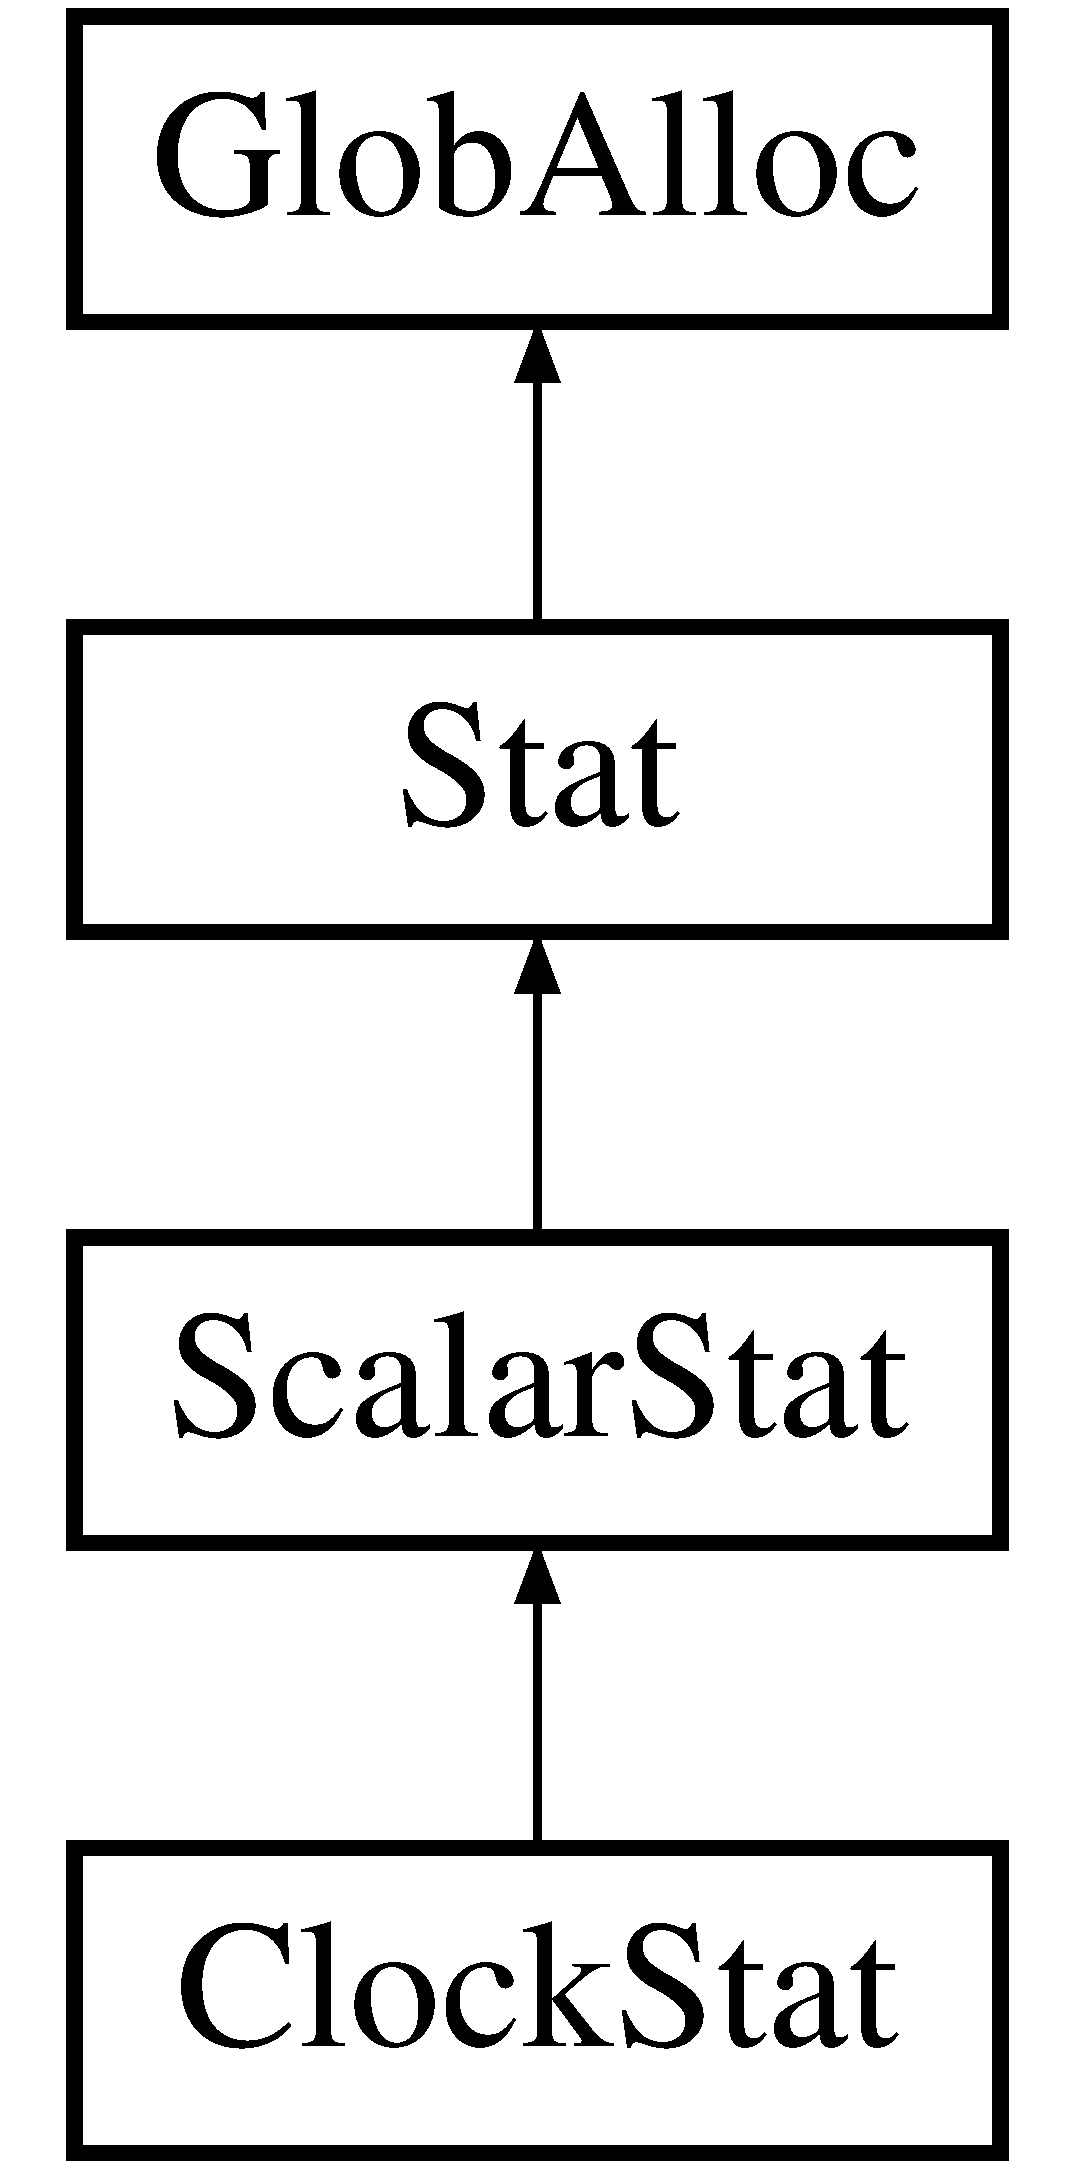
\includegraphics[height=4.000000cm]{classClockStat}
\end{center}
\end{figure}
\subsection*{Public Member Functions}
\begin{DoxyCompactItemize}
\item 
\hypertarget{classClockStat_aa45f73112d2c9f8ad79f33a50610577d}{void {\bfseries start} ()}\label{classClockStat_aa45f73112d2c9f8ad79f33a50610577d}

\item 
\hypertarget{classClockStat_a8bbe37eb00c3fe0fb0615df8e3f9f16a}{void {\bfseries end} ()}\label{classClockStat_a8bbe37eb00c3fe0fb0615df8e3f9f16a}

\item 
\hypertarget{classClockStat_ac5a756bd6bea1ade23d31630e1b5c0ca}{uint64\-\_\-t {\bfseries get} () const }\label{classClockStat_ac5a756bd6bea1ade23d31630e1b5c0ca}

\end{DoxyCompactItemize}
\subsection*{Additional Inherited Members}


The documentation for this class was generated from the following file\-:\begin{DoxyCompactItemize}
\item 
profile\-\_\-stats.\-h\end{DoxyCompactItemize}

\hypertarget{classConfig}{\section{Config Class Reference}
\label{classConfig}\index{Config@{Config}}
}
\subsection*{Public Member Functions}
\begin{DoxyCompactItemize}
\item 
\hypertarget{classConfig_a17ddbd4edf9e5f8e130bb85370f0d8b7}{{\bfseries Config} (const char $\ast$in\-File)}\label{classConfig_a17ddbd4edf9e5f8e130bb85370f0d8b7}

\item 
\hypertarget{classConfig_a541a794277a0f2ad86fb965ccd27a2ae}{void {\bfseries write\-And\-Close} (const char $\ast$out\-File, bool strict\-Check)}\label{classConfig_a541a794277a0f2ad86fb965ccd27a2ae}

\item 
\hypertarget{classConfig_ac5e2bc2c541d36f5441c84bf25649ef6}{bool {\bfseries exists} (const char $\ast$key)}\label{classConfig_ac5e2bc2c541d36f5441c84bf25649ef6}

\item 
\hypertarget{classConfig_a6d0453bf1e96d0390521efbb0e904523}{bool {\bfseries exists} (const std\-::string \&key)}\label{classConfig_a6d0453bf1e96d0390521efbb0e904523}

\item 
\hypertarget{classConfig_a52e4ff571be6515ecea0f1b14794087f}{{\footnotesize template$<$typename T $>$ }\\T {\bfseries get} (const char $\ast$key)}\label{classConfig_a52e4ff571be6515ecea0f1b14794087f}

\item 
\hypertarget{classConfig_aaa2d3de617583fbbc65b4bbc1778ed94}{{\footnotesize template$<$typename T $>$ }\\T {\bfseries get} (const std\-::string \&key)}\label{classConfig_aaa2d3de617583fbbc65b4bbc1778ed94}

\item 
\hypertarget{classConfig_a6034829eb5be47b7b9d6a3d90f3a4f67}{{\footnotesize template$<$typename T $>$ }\\T {\bfseries get} (const char $\ast$key, T def)}\label{classConfig_a6034829eb5be47b7b9d6a3d90f3a4f67}

\item 
\hypertarget{classConfig_a1389961bf83660636d1a09c0d3fcd12a}{{\footnotesize template$<$typename T $>$ }\\T {\bfseries get} (const std\-::string \&key, T def)}\label{classConfig_a1389961bf83660636d1a09c0d3fcd12a}

\item 
\hypertarget{classConfig_a27543c26c56e81e436ed3d3b533f4b6e}{void {\bfseries subgroups} (const char $\ast$key, std\-::vector$<$ const char $\ast$ $>$ \&grps)}\label{classConfig_a27543c26c56e81e436ed3d3b533f4b6e}

\item 
\hypertarget{classConfig_a3950588dcea9c919e7f6d58c4904514d}{void {\bfseries subgroups} (const std\-::string \&key, std\-::vector$<$ const char $\ast$ $>$ \&grps)}\label{classConfig_a3950588dcea9c919e7f6d58c4904514d}

\item 
\hypertarget{classConfig_a89ec1c95c45bfd3eedca3eb47d7e6b66}{{\footnotesize template$<$$>$ }\\uint32\-\_\-t {\bfseries get} (const char $\ast$key)}\label{classConfig_a89ec1c95c45bfd3eedca3eb47d7e6b66}

\item 
\hypertarget{classConfig_a83e49ae726af6b833f6d655471980426}{{\footnotesize template$<$$>$ }\\uint64\-\_\-t {\bfseries get} (const char $\ast$key)}\label{classConfig_a83e49ae726af6b833f6d655471980426}

\item 
\hypertarget{classConfig_a35b80ae4143a735dbb8cd979e31d9f30}{{\footnotesize template$<$$>$ }\\bool {\bfseries get} (const char $\ast$key)}\label{classConfig_a35b80ae4143a735dbb8cd979e31d9f30}

\item 
\hypertarget{classConfig_a868b65b13b4d843b22126a73e0d119b4}{{\footnotesize template$<$$>$ }\\const char $\ast$ {\bfseries get} (const char $\ast$key)}\label{classConfig_a868b65b13b4d843b22126a73e0d119b4}

\item 
\hypertarget{classConfig_a9fb644c76122da00f0396cca69fdb854}{{\footnotesize template$<$$>$ }\\double {\bfseries get} (const char $\ast$key)}\label{classConfig_a9fb644c76122da00f0396cca69fdb854}

\item 
\hypertarget{classConfig_a01503b0fe03e702ac42cc71025496cc7}{{\footnotesize template$<$$>$ }\\uint32\-\_\-t {\bfseries get} (const char $\ast$key, uint32\-\_\-t def)}\label{classConfig_a01503b0fe03e702ac42cc71025496cc7}

\item 
\hypertarget{classConfig_ab7c8f41f1f68386d5c5aa220b04a6395}{{\footnotesize template$<$$>$ }\\uint64\-\_\-t {\bfseries get} (const char $\ast$key, uint64\-\_\-t def)}\label{classConfig_ab7c8f41f1f68386d5c5aa220b04a6395}

\item 
\hypertarget{classConfig_aeb1e3d9528ac85d99ac240c127a230fe}{{\footnotesize template$<$$>$ }\\bool {\bfseries get} (const char $\ast$key, bool def)}\label{classConfig_aeb1e3d9528ac85d99ac240c127a230fe}

\item 
\hypertarget{classConfig_a7d43af7622dab5c20df7a02d0438db0f}{{\footnotesize template$<$$>$ }\\const char $\ast$ {\bfseries get} (const char $\ast$key, const char $\ast$def)}\label{classConfig_a7d43af7622dab5c20df7a02d0438db0f}

\item 
\hypertarget{classConfig_ae495cbb8c0575c30e9539d8ed6082a72}{{\footnotesize template$<$$>$ }\\double {\bfseries get} (const char $\ast$key, double def)}\label{classConfig_ae495cbb8c0575c30e9539d8ed6082a72}

\end{DoxyCompactItemize}


The documentation for this class was generated from the following files\-:\begin{DoxyCompactItemize}
\item 
config.\-h\item 
config.\-cpp\end{DoxyCompactItemize}

\hypertarget{classContentionSim}{\section{Contention\-Sim Class Reference}
\label{classContentionSim}\index{Contention\-Sim@{Contention\-Sim}}
}
Inheritance diagram for Contention\-Sim\-:\begin{figure}[H]
\begin{center}
\leavevmode
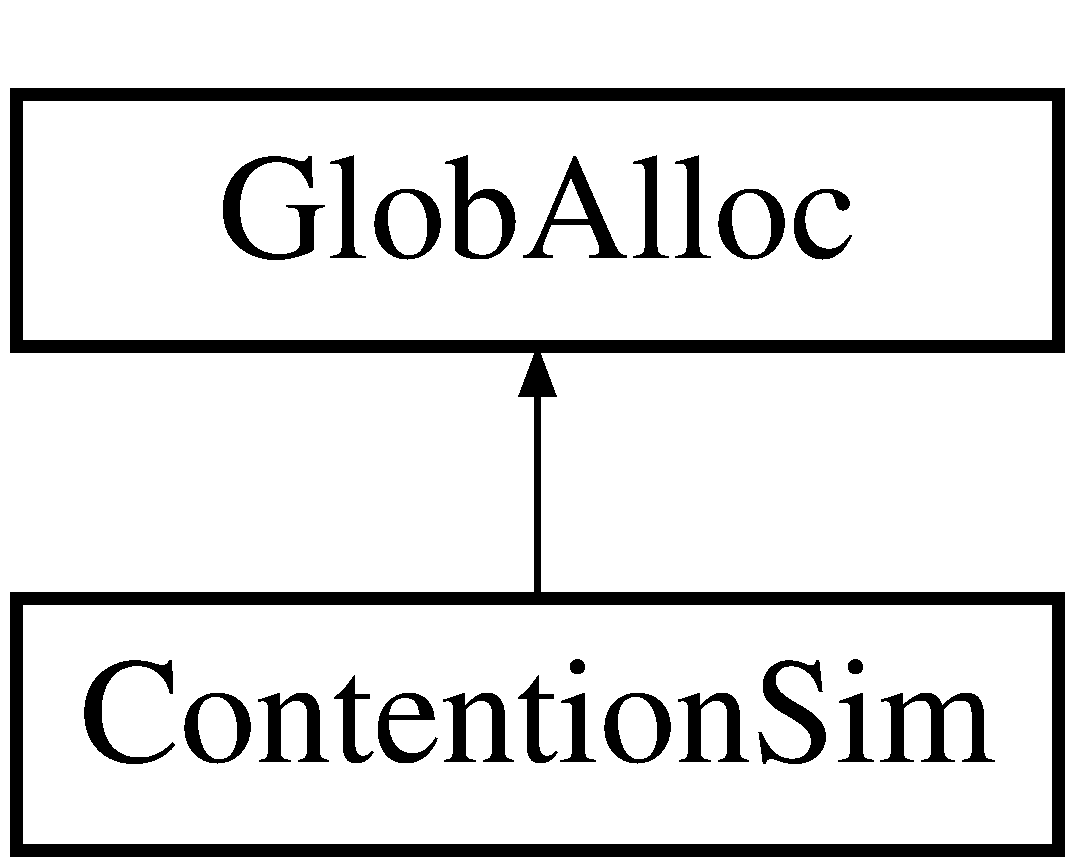
\includegraphics[height=2.000000cm]{classContentionSim}
\end{center}
\end{figure}
\subsection*{Public Member Functions}
\begin{DoxyCompactItemize}
\item 
\hypertarget{classContentionSim_a4c7d65f216bc7cd5b4db0f4736d269d3}{{\bfseries Contention\-Sim} (uint32\-\_\-t \-\_\-num\-Domains, uint32\-\_\-t \-\_\-num\-Sim\-Threads)}\label{classContentionSim_a4c7d65f216bc7cd5b4db0f4736d269d3}

\item 
\hypertarget{classContentionSim_a43f3141595b3d9ea5e067ce8ce74d79c}{void {\bfseries init\-Stats} (\hyperlink{classAggregateStat}{Aggregate\-Stat} $\ast$parent\-Stat)}\label{classContentionSim_a43f3141595b3d9ea5e067ce8ce74d79c}

\item 
\hypertarget{classContentionSim_a5fc392e200bc8c0acada32e838420ecc}{void {\bfseries post\-Init} ()}\label{classContentionSim_a5fc392e200bc8c0acada32e838420ecc}

\item 
\hypertarget{classContentionSim_a1cd640e573094fb670fc8b83f4a07332}{void {\bfseries enqueue} (\hyperlink{classTimingEvent}{Timing\-Event} $\ast$ev, uint64\-\_\-t cycle)}\label{classContentionSim_a1cd640e573094fb670fc8b83f4a07332}

\item 
\hypertarget{classContentionSim_aade85cbc1438a43581a34036fc79bb12}{void {\bfseries enqueue\-Synced} (\hyperlink{classTimingEvent}{Timing\-Event} $\ast$ev, uint64\-\_\-t cycle)}\label{classContentionSim_aade85cbc1438a43581a34036fc79bb12}

\item 
\hypertarget{classContentionSim_a4c06e1040f29e473b080f80fb80b8230}{void {\bfseries enqueue\-Crossing} (\hyperlink{classCrossingEvent}{Crossing\-Event} $\ast$ev, uint64\-\_\-t cycle, uint32\-\_\-t src\-Id, uint32\-\_\-t src\-Domain, uint32\-\_\-t dst\-Domain, \hyperlink{classEventRecorder}{Event\-Recorder} $\ast$ev\-Rec)}\label{classContentionSim_a4c06e1040f29e473b080f80fb80b8230}

\item 
\hypertarget{classContentionSim_a961f4d3a18597d2413188a67cb800ee5}{void {\bfseries simulate\-Phase} (uint64\-\_\-t limit)}\label{classContentionSim_a961f4d3a18597d2413188a67cb800ee5}

\item 
\hypertarget{classContentionSim_a0d5aeadd8d3270a37ef7dcf79488621d}{void {\bfseries finish} ()}\label{classContentionSim_a0d5aeadd8d3270a37ef7dcf79488621d}

\item 
\hypertarget{classContentionSim_ae9982a572df654edb1bf6a7f5f0d2197}{uint64\-\_\-t {\bfseries get\-Last\-Limit} ()}\label{classContentionSim_ae9982a572df654edb1bf6a7f5f0d2197}

\item 
\hypertarget{classContentionSim_a782a5b4f4f1d980cd781ef9b87c2c7c3}{uint64\-\_\-t {\bfseries get\-Cur\-Cycle} (uint32\-\_\-t domain)}\label{classContentionSim_a782a5b4f4f1d980cd781ef9b87c2c7c3}

\item 
\hypertarget{classContentionSim_aff58f59d88d745695f24441f08fc0eb8}{void {\bfseries set\-Prio} (uint32\-\_\-t domain, uint32\-\_\-t prio)}\label{classContentionSim_aff58f59d88d745695f24441f08fc0eb8}

\end{DoxyCompactItemize}


The documentation for this class was generated from the following files\-:\begin{DoxyCompactItemize}
\item 
contention\-\_\-sim.\-h\item 
contention\-\_\-sim.\-cpp\end{DoxyCompactItemize}

\hypertarget{classCore}{\section{Core Class Reference}
\label{classCore}\index{Core@{Core}}
}
Inheritance diagram for Core\-:\begin{figure}[H]
\begin{center}
\leavevmode
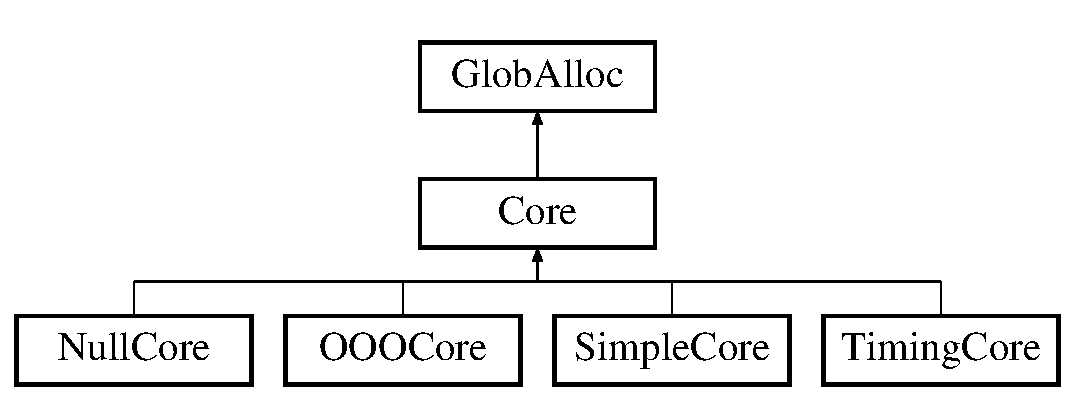
\includegraphics[height=3.000000cm]{classCore}
\end{center}
\end{figure}
\subsection*{Public Member Functions}
\begin{DoxyCompactItemize}
\item 
\hypertarget{classCore_ab977c051264daa466362c38f20bf7512}{{\bfseries Core} (g\-\_\-string \&\-\_\-name)}\label{classCore_ab977c051264daa466362c38f20bf7512}

\item 
\hypertarget{classCore_ac3fa041719ceb8c63958eb834eb67c99}{virtual uint64\-\_\-t {\bfseries get\-Instrs} () const =0}\label{classCore_ac3fa041719ceb8c63958eb834eb67c99}

\item 
\hypertarget{classCore_ac47f10ddfe0e591620113e0fe2ae2351}{virtual uint64\-\_\-t {\bfseries get\-Phase\-Cycles} () const =0}\label{classCore_ac47f10ddfe0e591620113e0fe2ae2351}

\item 
\hypertarget{classCore_ac2e4ef43c71b1e50a3cc89d1ec8c58aa}{virtual uint64\-\_\-t {\bfseries get\-Cycles} () const =0}\label{classCore_ac2e4ef43c71b1e50a3cc89d1ec8c58aa}

\item 
\hypertarget{classCore_a093c22041db0e412cf0c84c862676629}{virtual void {\bfseries init\-Stats} (\hyperlink{classAggregateStat}{Aggregate\-Stat} $\ast$parent\-Stat)=0}\label{classCore_a093c22041db0e412cf0c84c862676629}

\item 
\hypertarget{classCore_a9e0d130d0746bed33473dcd8cbc397bb}{virtual void {\bfseries context\-Switch} (int32\-\_\-t gid)=0}\label{classCore_a9e0d130d0746bed33473dcd8cbc397bb}

\item 
\hypertarget{classCore_abf2a30c06a88df1382a7d0cf0da08d2c}{virtual void {\bfseries leave} ()}\label{classCore_abf2a30c06a88df1382a7d0cf0da08d2c}

\item 
\hypertarget{classCore_a2e692b0643767e9abf6b94794cd0c388}{virtual void {\bfseries join} ()}\label{classCore_a2e692b0643767e9abf6b94794cd0c388}

\item 
\hypertarget{classCore_acf1335c8e2215e3e1ff91aa71359f4ec}{virtual \hyperlink{structInstrFuncPtrs}{Instr\-Func\-Ptrs} {\bfseries Get\-Func\-Ptrs} ()=0}\label{classCore_acf1335c8e2215e3e1ff91aa71359f4ec}

\end{DoxyCompactItemize}
\subsection*{Protected Attributes}
\begin{DoxyCompactItemize}
\item 
\hypertarget{classCore_af9a530c13a24af172b2430b9b53ee7e3}{g\-\_\-string {\bfseries name}}\label{classCore_af9a530c13a24af172b2430b9b53ee7e3}

\end{DoxyCompactItemize}


The documentation for this class was generated from the following file\-:\begin{DoxyCompactItemize}
\item 
core.\-h\end{DoxyCompactItemize}

\hypertarget{classCorePartMapper}{\section{Core\-Part\-Mapper Class Reference}
\label{classCorePartMapper}\index{Core\-Part\-Mapper@{Core\-Part\-Mapper}}
}
Inheritance diagram for Core\-Part\-Mapper\-:\begin{figure}[H]
\begin{center}
\leavevmode
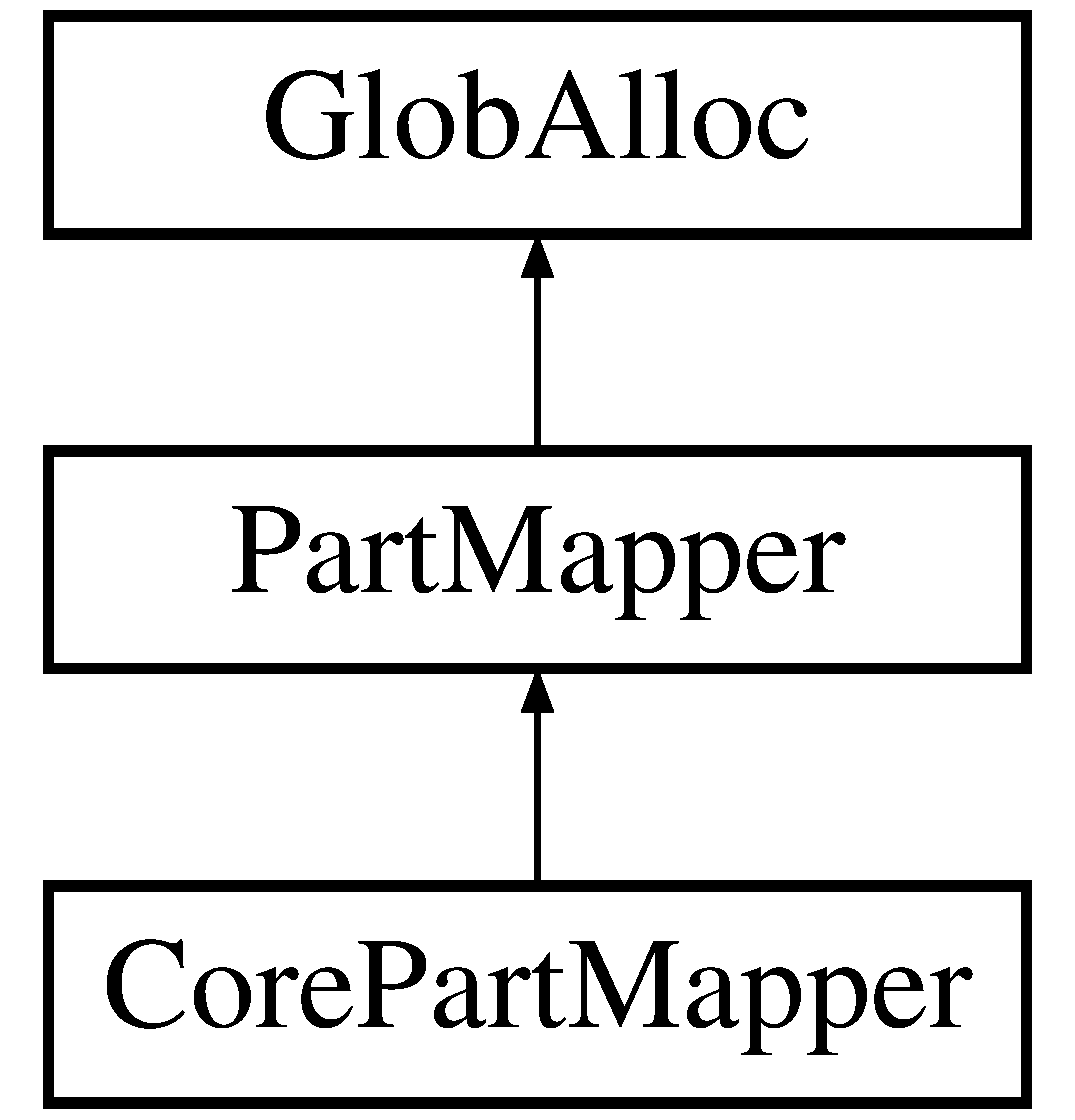
\includegraphics[height=3.000000cm]{classCorePartMapper}
\end{center}
\end{figure}
\subsection*{Public Member Functions}
\begin{DoxyCompactItemize}
\item 
\hypertarget{classCorePartMapper_ab235c7372cb858fa493ea760fa46c3a1}{{\bfseries Core\-Part\-Mapper} (uint32\-\_\-t \-\_\-num\-Cores)}\label{classCorePartMapper_ab235c7372cb858fa493ea760fa46c3a1}

\item 
\hypertarget{classCorePartMapper_a687d08f86d047782501b81fbc366fd50}{virtual uint32\-\_\-t {\bfseries get\-Num\-Partitions} ()}\label{classCorePartMapper_a687d08f86d047782501b81fbc366fd50}

\item 
virtual uint32\-\_\-t \hyperlink{classCorePartMapper_a37c35ce6508de5e769dd138f47d8c760}{get\-Partition} (const \hyperlink{structMemReq}{Mem\-Req} \&req)
\end{DoxyCompactItemize}


\subsection{Member Function Documentation}
\hypertarget{classCorePartMapper_a37c35ce6508de5e769dd138f47d8c760}{\index{Core\-Part\-Mapper@{Core\-Part\-Mapper}!get\-Partition@{get\-Partition}}
\index{get\-Partition@{get\-Partition}!CorePartMapper@{Core\-Part\-Mapper}}
\subsubsection[{get\-Partition}]{\setlength{\rightskip}{0pt plus 5cm}uint32\-\_\-t Core\-Part\-Mapper\-::get\-Partition (
\begin{DoxyParamCaption}
\item[{const {\bf Mem\-Req} \&}]{req}
\end{DoxyParamCaption}
)\hspace{0.3cm}{\ttfamily [virtual]}}}\label{classCorePartMapper_a37c35ce6508de5e769dd138f47d8c760}
\$lic\$ Copyright (C) 2012-\/2015 by Massachusetts Institute of Technology Copyright (C) 2010-\/2013 by The Board of Trustees of Stanford University

This file is part of zsim.

zsim is free software; you can redistribute it and/or modify it under the terms of the G\-N\-U General Public License as published by the Free Software Foundation, version 2.

If you use this software in your research, we request that you reference the zsim paper (\char`\"{}\-Z\-Sim\-: Fast and Accurate Microarchitectural Simulation of
\-Thousand-\/\-Core Systems\char`\"{}, Sanchez and Kozyrakis, I\-S\-C\-A-\/40, June 2013) as the source of the simulator in any publications that use this software, and that you send us a citation of your work.

zsim is distributed in the hope that it will be useful, but W\-I\-T\-H\-O\-U\-T A\-N\-Y W\-A\-R\-R\-A\-N\-T\-Y; without even the implied warranty of M\-E\-R\-C\-H\-A\-N\-T\-A\-B\-I\-L\-I\-T\-Y or F\-I\-T\-N\-E\-S\-S F\-O\-R A P\-A\-R\-T\-I\-C\-U\-L\-A\-R P\-U\-R\-P\-O\-S\-E. See the G\-N\-U General Public License for more details.

You should have received a copy of the G\-N\-U General Public License along with this program. If not, see \href{http://www.gnu.org/licenses/}{\tt http\-://www.\-gnu.\-org/licenses/}. 

Implements \hyperlink{classPartMapper}{Part\-Mapper}.



The documentation for this class was generated from the following files\-:\begin{DoxyCompactItemize}
\item 
partition\-\_\-mapper.\-h\item 
partition\-\_\-mapper.\-cpp\end{DoxyCompactItemize}

\hypertarget{classCoreRecorder}{\section{Core\-Recorder Class Reference}
\label{classCoreRecorder}\index{Core\-Recorder@{Core\-Recorder}}
}
\subsection*{Public Member Functions}
\begin{DoxyCompactItemize}
\item 
\hypertarget{classCoreRecorder_a9817e576d86284d031cfdde850421465}{{\bfseries Core\-Recorder} (uint32\-\_\-t \-\_\-domain, g\-\_\-string \&\-\_\-name)}\label{classCoreRecorder_a9817e576d86284d031cfdde850421465}

\item 
\hypertarget{classCoreRecorder_a75258d05bd878d2c24692ea126fa0fca}{uint64\-\_\-t {\bfseries notify\-Join} (uint64\-\_\-t cur\-Cycle)}\label{classCoreRecorder_a75258d05bd878d2c24692ea126fa0fca}

\item 
\hypertarget{classCoreRecorder_a5de90ebbe596f875c59b876c25ac5e4e}{void {\bfseries notify\-Leave} (uint64\-\_\-t cur\-Cycle)}\label{classCoreRecorder_a5de90ebbe596f875c59b876c25ac5e4e}

\item 
\hypertarget{classCoreRecorder_a6bb5ab211da547753d433832c30324f3}{void {\bfseries record} (uint64\-\_\-t start\-Cycle)}\label{classCoreRecorder_a6bb5ab211da547753d433832c30324f3}

\item 
\hypertarget{classCoreRecorder_a3b68c6854d37e643982f1111d4244e9f}{uint64\-\_\-t {\bfseries c\-Sim\-Start} (uint64\-\_\-t cur\-Cycle)}\label{classCoreRecorder_a3b68c6854d37e643982f1111d4244e9f}

\item 
\hypertarget{classCoreRecorder_ac09b4e16164bce69aa47bda2e406b61d}{uint64\-\_\-t {\bfseries c\-Sim\-End} (uint64\-\_\-t cur\-Cycle)}\label{classCoreRecorder_ac09b4e16164bce69aa47bda2e406b61d}

\item 
\hypertarget{classCoreRecorder_a225bf52a8b8655954392caa90a2ae5df}{void {\bfseries report\-Event\-Simulated} (\hyperlink{classTimingCoreEvent}{Timing\-Core\-Event} $\ast$ev)}\label{classCoreRecorder_a225bf52a8b8655954392caa90a2ae5df}

\item 
\hypertarget{classCoreRecorder_a2d23b6db5507453886f42deee7150994}{\hyperlink{classEventRecorder}{Event\-Recorder} $\ast$ {\bfseries get\-Event\-Recorder} ()}\label{classCoreRecorder_a2d23b6db5507453886f42deee7150994}

\item 
\hypertarget{classCoreRecorder_ae30f7a903534b835fb3eae65728e903f}{uint64\-\_\-t {\bfseries get\-Unhalted\-Cycles} (uint64\-\_\-t cur\-Cycle) const }\label{classCoreRecorder_ae30f7a903534b835fb3eae65728e903f}

\item 
\hypertarget{classCoreRecorder_a3f0d400abd3c59e92dad3424b3319400}{uint64\-\_\-t {\bfseries get\-Contention\-Cycles} () const }\label{classCoreRecorder_a3f0d400abd3c59e92dad3424b3319400}

\end{DoxyCompactItemize}


The documentation for this class was generated from the following files\-:\begin{DoxyCompactItemize}
\item 
core\-\_\-recorder.\-h\item 
core\-\_\-recorder.\-cpp\end{DoxyCompactItemize}

\hypertarget{classCounter}{\section{Counter Class Reference}
\label{classCounter}\index{Counter@{Counter}}
}
Inheritance diagram for Counter\-:\begin{figure}[H]
\begin{center}
\leavevmode
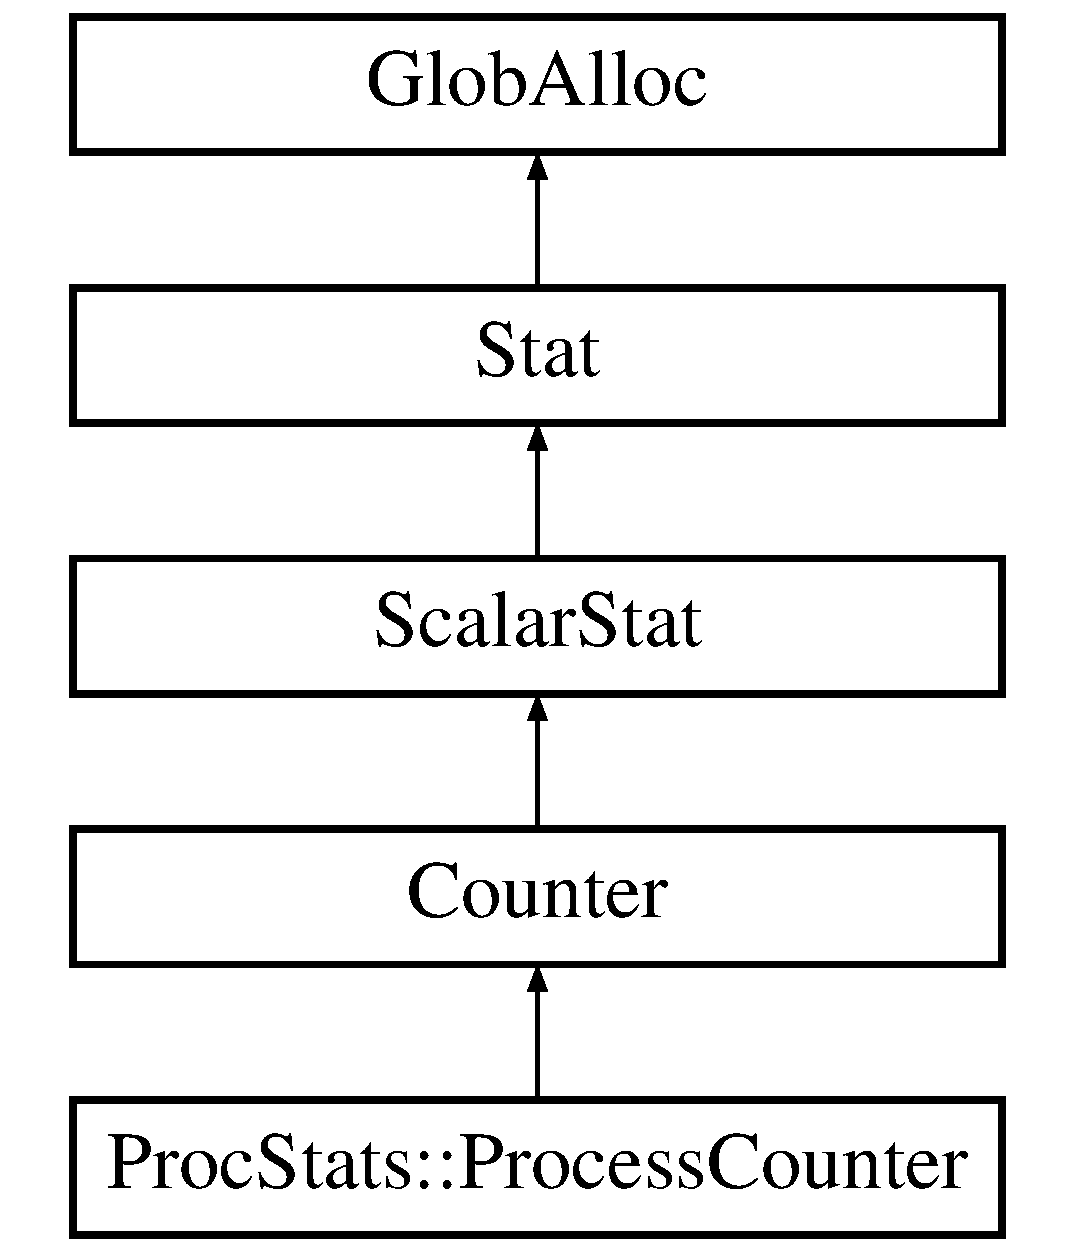
\includegraphics[height=5.000000cm]{classCounter}
\end{center}
\end{figure}
\subsection*{Public Member Functions}
\begin{DoxyCompactItemize}
\item 
\hypertarget{classCounter_af4d8fe24c5d69c0a90053952947a0784}{void {\bfseries init} (const char $\ast$name, const char $\ast$desc)}\label{classCounter_af4d8fe24c5d69c0a90053952947a0784}

\item 
\hypertarget{classCounter_a3d22d44790be17cb3819593dbdd61982}{void {\bfseries inc} (uint64\-\_\-t delta)}\label{classCounter_a3d22d44790be17cb3819593dbdd61982}

\item 
\hypertarget{classCounter_a936f247406df26f76e06aed14fab9713}{void {\bfseries inc} ()}\label{classCounter_a936f247406df26f76e06aed14fab9713}

\item 
\hypertarget{classCounter_ac5e80a29c4063ab0faef1c25d31f48ed}{void {\bfseries atomic\-Inc} (uint64\-\_\-t delta)}\label{classCounter_ac5e80a29c4063ab0faef1c25d31f48ed}

\item 
\hypertarget{classCounter_a937c25ffb0c2049d293cb480ce5aa155}{void {\bfseries atomic\-Inc} ()}\label{classCounter_a937c25ffb0c2049d293cb480ce5aa155}

\item 
\hypertarget{classCounter_a7af39c45db59374d9fb96cdebae210bc}{uint64\-\_\-t {\bfseries get} () const }\label{classCounter_a7af39c45db59374d9fb96cdebae210bc}

\item 
\hypertarget{classCounter_afeff3d9b8fa53c0bd7ea8b36363a478a}{void {\bfseries set} (uint64\-\_\-t data)}\label{classCounter_afeff3d9b8fa53c0bd7ea8b36363a478a}

\end{DoxyCompactItemize}
\subsection*{Additional Inherited Members}


The documentation for this class was generated from the following file\-:\begin{DoxyCompactItemize}
\item 
stats.\-h\end{DoxyCompactItemize}

\hypertarget{structCpuIdRecord}{\section{Cpu\-Id\-Record Struct Reference}
\label{structCpuIdRecord}\index{Cpu\-Id\-Record@{Cpu\-Id\-Record}}
}


{\ttfamily \#include $<$cpuid.\-h$>$}

\subsection*{Public Member Functions}
\begin{DoxyCompactItemize}
\item 
\hypertarget{structCpuIdRecord_ac22508a164c283b85b40a5fd252bb717}{bool {\bfseries operator$<$} (const \hyperlink{structCpuIdRecord}{Cpu\-Id\-Record} \&other) const }\label{structCpuIdRecord_ac22508a164c283b85b40a5fd252bb717}

\end{DoxyCompactItemize}
\subsection*{Public Attributes}
\begin{DoxyCompactItemize}
\item 
\hypertarget{structCpuIdRecord_a29cb7064576934fde031217dc72748eb}{unsigned {\bfseries eax\-In}}\label{structCpuIdRecord_a29cb7064576934fde031217dc72748eb}

\item 
\hypertarget{structCpuIdRecord_a0550345b9fca22f5a71f562cf9aa798b}{unsigned {\bfseries ecx\-In}}\label{structCpuIdRecord_a0550345b9fca22f5a71f562cf9aa798b}

\item 
\hypertarget{structCpuIdRecord_a00980ac5f6f5843e58347584158bbfb3}{unsigned {\bfseries eax}}\label{structCpuIdRecord_a00980ac5f6f5843e58347584158bbfb3}

\item 
\hypertarget{structCpuIdRecord_a54bcb48b9c8c83ac59fc529a31b5090a}{unsigned {\bfseries ebx}}\label{structCpuIdRecord_a54bcb48b9c8c83ac59fc529a31b5090a}

\item 
\hypertarget{structCpuIdRecord_ac19e67764ed1acc358e9326582bbc82f}{unsigned {\bfseries ecx}}\label{structCpuIdRecord_ac19e67764ed1acc358e9326582bbc82f}

\item 
\hypertarget{structCpuIdRecord_a7e89950c616061d3031f1298eaf436d5}{unsigned {\bfseries edx}}\label{structCpuIdRecord_a7e89950c616061d3031f1298eaf436d5}

\end{DoxyCompactItemize}


\subsection{Detailed Description}
\$lic\$ Copyright (C) 2012-\/2015 by Massachusetts Institute of Technology Copyright (C) 2010-\/2013 by The Board of Trustees of Stanford University

This file is part of zsim.

zsim is free software; you can redistribute it and/or modify it under the terms of the G\-N\-U General Public License as published by the Free Software Foundation, version 2.

If you use this software in your research, we request that you reference the zsim paper (\char`\"{}\-Z\-Sim\-: Fast and Accurate Microarchitectural Simulation of
\-Thousand-\/\-Core Systems\char`\"{}, Sanchez and Kozyrakis, I\-S\-C\-A-\/40, June 2013) as the source of the simulator in any publications that use this software, and that you send us a citation of your work.

zsim is distributed in the hope that it will be useful, but W\-I\-T\-H\-O\-U\-T A\-N\-Y W\-A\-R\-R\-A\-N\-T\-Y; without even the implied warranty of M\-E\-R\-C\-H\-A\-N\-T\-A\-B\-I\-L\-I\-T\-Y or F\-I\-T\-N\-E\-S\-S F\-O\-R A P\-A\-R\-T\-I\-C\-U\-L\-A\-R P\-U\-R\-P\-O\-S\-E. See the G\-N\-U General Public License for more details.

You should have received a copy of the G\-N\-U General Public License along with this program. If not, see \href{http://www.gnu.org/licenses/}{\tt http\-://www.\-gnu.\-org/licenses/}. 

The documentation for this struct was generated from the following file\-:\begin{DoxyCompactItemize}
\item 
cpuid.\-h\end{DoxyCompactItemize}

\hypertarget{classCrossingEvent}{\section{Crossing\-Event Class Reference}
\label{classCrossingEvent}\index{Crossing\-Event@{Crossing\-Event}}
}
Inheritance diagram for Crossing\-Event\-:\begin{figure}[H]
\begin{center}
\leavevmode
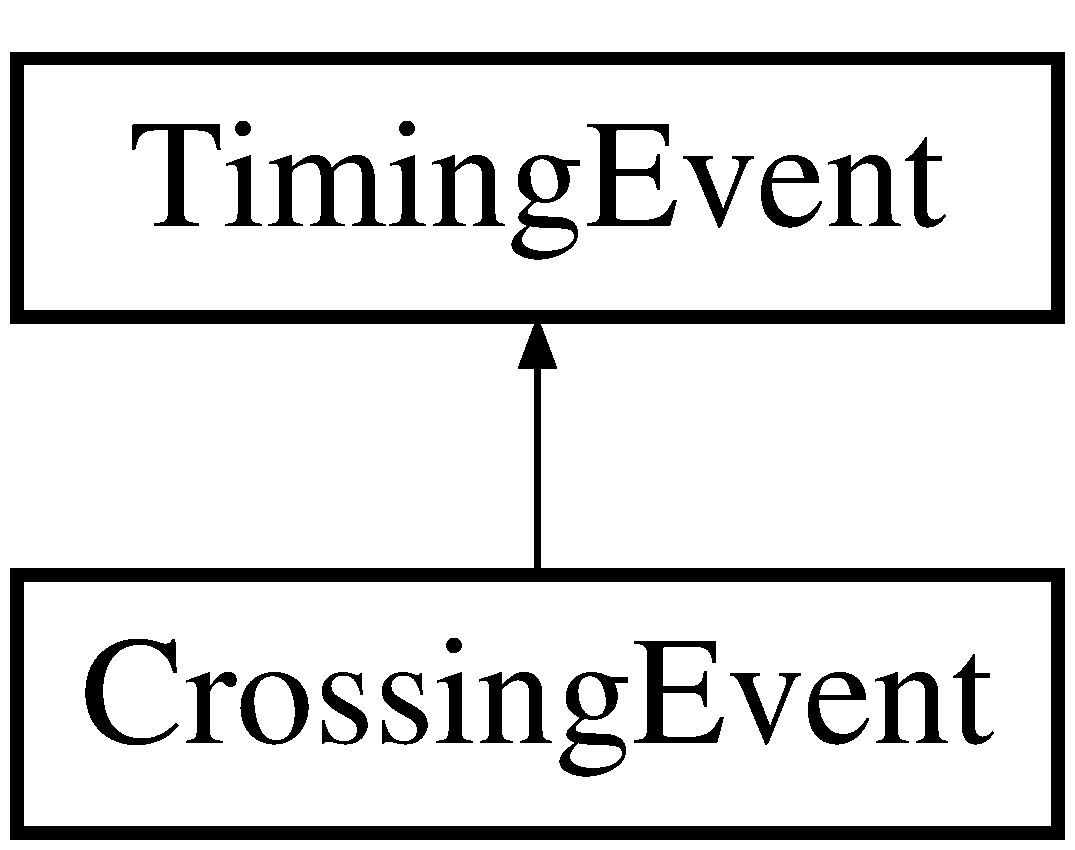
\includegraphics[height=2.000000cm]{classCrossingEvent}
\end{center}
\end{figure}
\subsection*{Public Member Functions}
\begin{DoxyCompactItemize}
\item 
\hypertarget{classCrossingEvent_ab3416373c80cc905faaf615d69b539ed}{{\bfseries Crossing\-Event} (\hyperlink{classTimingEvent}{Timing\-Event} $\ast$parent, \hyperlink{classTimingEvent}{Timing\-Event} $\ast$child, uint64\-\_\-t \-\_\-min\-Start\-Cycle, \hyperlink{classEventRecorder}{Event\-Recorder} $\ast$\-\_\-ev\-Rec)}\label{classCrossingEvent_ab3416373c80cc905faaf615d69b539ed}

\item 
\hypertarget{classCrossingEvent_a275b5945ada8e357a0c07cf2428b9460}{\hyperlink{classTimingEvent}{Timing\-Event} $\ast$ {\bfseries get\-Src\-Domain\-Event} ()}\label{classCrossingEvent_a275b5945ada8e357a0c07cf2428b9460}

\item 
virtual void \hyperlink{classCrossingEvent_a96199fafd70da779df838f73f24cb6b5}{parent\-Done} (uint64\-\_\-t start\-Cycle)
\item 
\hypertarget{classCrossingEvent_a2ca00bf0b21769af20bc64b287bfaf74}{virtual void {\bfseries simulate} (uint64\-\_\-t sim\-Cycle)}\label{classCrossingEvent_a2ca00bf0b21769af20bc64b287bfaf74}

\end{DoxyCompactItemize}
\subsection*{Friends}
\begin{DoxyCompactItemize}
\item 
\hypertarget{classCrossingEvent_a96b81ec5d9f4b197024c5bd08fc10c38}{class {\bfseries Contention\-Sim}}\label{classCrossingEvent_a96b81ec5d9f4b197024c5bd08fc10c38}

\end{DoxyCompactItemize}
\subsection*{Additional Inherited Members}


\subsection{Member Function Documentation}
\hypertarget{classCrossingEvent_a96199fafd70da779df838f73f24cb6b5}{\index{Crossing\-Event@{Crossing\-Event}!parent\-Done@{parent\-Done}}
\index{parent\-Done@{parent\-Done}!CrossingEvent@{Crossing\-Event}}
\subsubsection[{parent\-Done}]{\setlength{\rightskip}{0pt plus 5cm}void Crossing\-Event\-::parent\-Done (
\begin{DoxyParamCaption}
\item[{uint64\-\_\-t}]{start\-Cycle}
\end{DoxyParamCaption}
)\hspace{0.3cm}{\ttfamily [virtual]}}}\label{classCrossingEvent_a96199fafd70da779df838f73f24cb6b5}
\$lic\$ Copyright (C) 2012-\/2015 by Massachusetts Institute of Technology Copyright (C) 2010-\/2013 by The Board of Trustees of Stanford University

This file is part of zsim.

zsim is free software; you can redistribute it and/or modify it under the terms of the G\-N\-U General Public License as published by the Free Software Foundation, version 2.

If you use this software in your research, we request that you reference the zsim paper (\char`\"{}\-Z\-Sim\-: Fast and Accurate Microarchitectural Simulation of
\-Thousand-\/\-Core Systems\char`\"{}, Sanchez and Kozyrakis, I\-S\-C\-A-\/40, June 2013) as the source of the simulator in any publications that use this software, and that you send us a citation of your work.

zsim is distributed in the hope that it will be useful, but W\-I\-T\-H\-O\-U\-T A\-N\-Y W\-A\-R\-R\-A\-N\-T\-Y; without even the implied warranty of M\-E\-R\-C\-H\-A\-N\-T\-A\-B\-I\-L\-I\-T\-Y or F\-I\-T\-N\-E\-S\-S F\-O\-R A P\-A\-R\-T\-I\-C\-U\-L\-A\-R P\-U\-R\-P\-O\-S\-E. See the G\-N\-U General Public License for more details.

You should have received a copy of the G\-N\-U General Public License along with this program. If not, see \href{http://www.gnu.org/licenses/}{\tt http\-://www.\-gnu.\-org/licenses/}. 

Reimplemented from \hyperlink{classTimingEvent_a55e7e2942d6607eb2a9dd484baf39070}{Timing\-Event}.



The documentation for this class was generated from the following files\-:\begin{DoxyCompactItemize}
\item 
timing\-\_\-event.\-h\item 
timing\-\_\-event.\-cpp\end{DoxyCompactItemize}

\hypertarget{classCycleBreakdownStat}{\section{Cycle\-Breakdown\-Stat Class Reference}
\label{classCycleBreakdownStat}\index{Cycle\-Breakdown\-Stat@{Cycle\-Breakdown\-Stat}}
}


{\ttfamily \#include $<$breakdown\-\_\-stats.\-h$>$}

Inheritance diagram for Cycle\-Breakdown\-Stat\-:\begin{figure}[H]
\begin{center}
\leavevmode
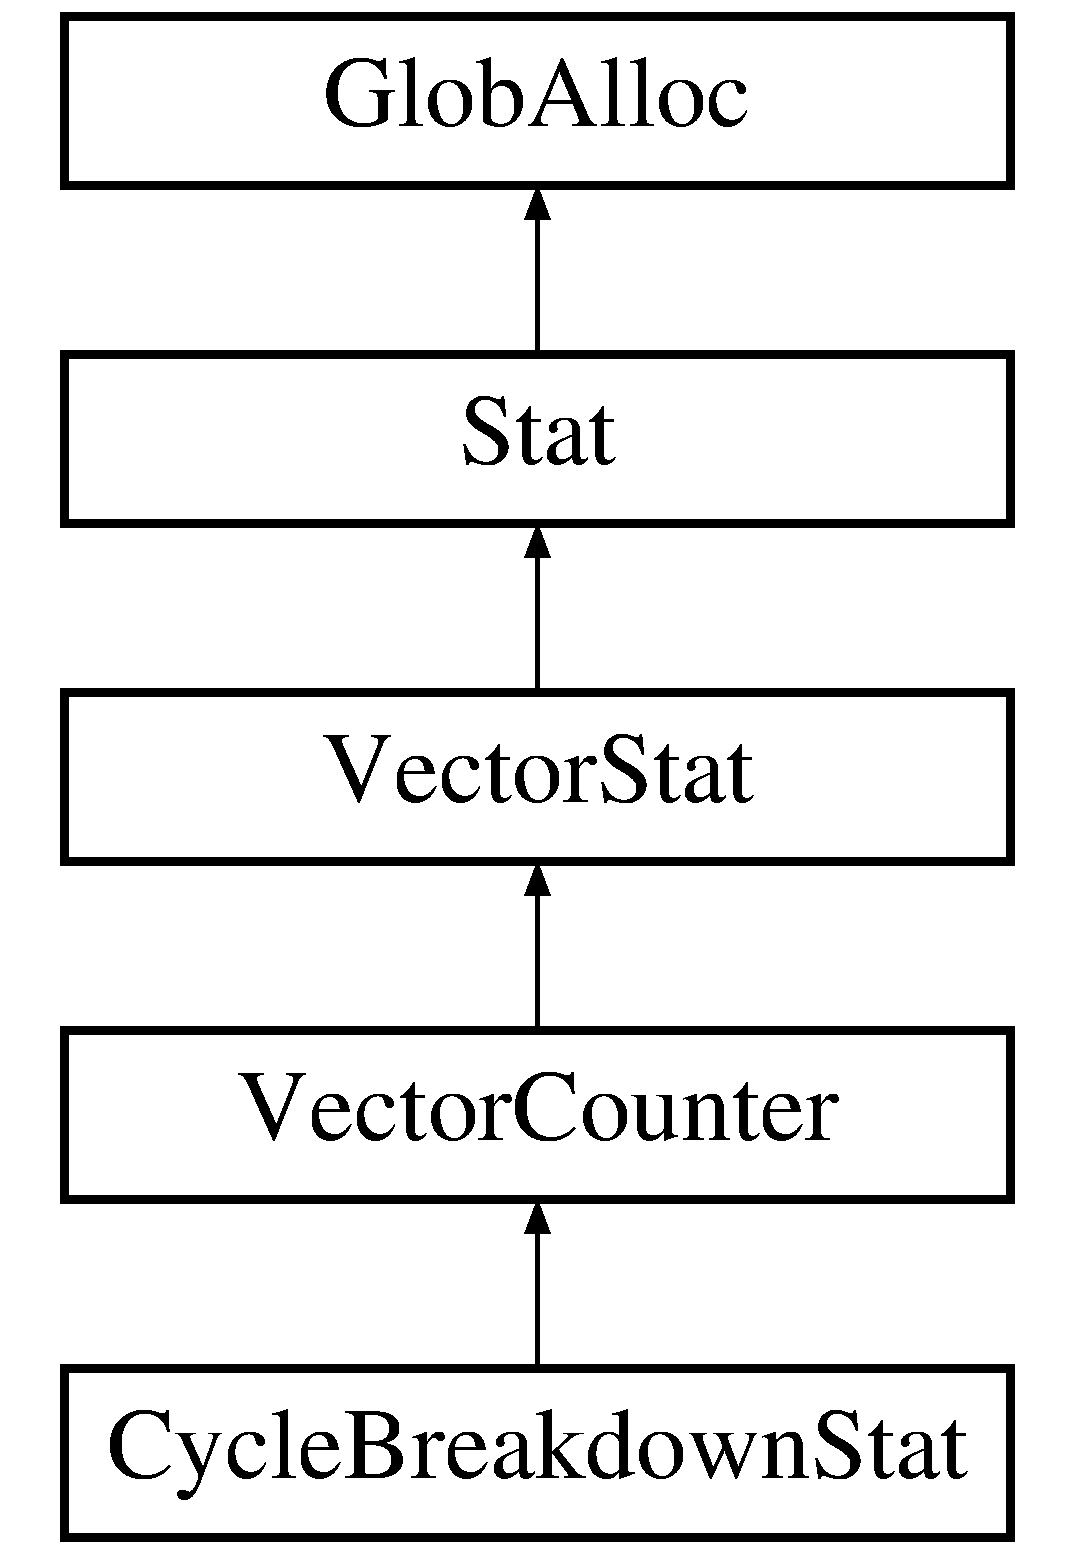
\includegraphics[height=5.000000cm]{classCycleBreakdownStat}
\end{center}
\end{figure}
\subsection*{Public Member Functions}
\begin{DoxyCompactItemize}
\item 
\hypertarget{classCycleBreakdownStat_ae82676301f6d9fdf98d6f5605fa7f134}{virtual void {\bfseries init} (const char $\ast$name, const char $\ast$desc, uint32\-\_\-t size)}\label{classCycleBreakdownStat_ae82676301f6d9fdf98d6f5605fa7f134}

\item 
\hypertarget{classCycleBreakdownStat_af939f01118305ad8f50359b429fab8a7}{virtual void {\bfseries init} (const char $\ast$name, const char $\ast$desc, uint32\-\_\-t size, const char $\ast$$\ast$names)}\label{classCycleBreakdownStat_af939f01118305ad8f50359b429fab8a7}

\item 
\hypertarget{classCycleBreakdownStat_aec2e256c006156472689efd6e5b98e49}{void {\bfseries transition} (uint32\-\_\-t new\-State, uint64\-\_\-t cycle)}\label{classCycleBreakdownStat_aec2e256c006156472689efd6e5b98e49}

\item 
\hypertarget{classCycleBreakdownStat_a04f433528adb05a600e3a319315f2a9d}{virtual uint64\-\_\-t {\bfseries count} (uint32\-\_\-t idx) const }\label{classCycleBreakdownStat_a04f433528adb05a600e3a319315f2a9d}

\end{DoxyCompactItemize}
\subsection*{Additional Inherited Members}


\subsection{Detailed Description}
\$lic\$ Copyright (C) 2012-\/2015 by Massachusetts Institute of Technology Copyright (C) 2010-\/2013 by The Board of Trustees of Stanford University

This file is part of zsim.

zsim is free software; you can redistribute it and/or modify it under the terms of the G\-N\-U General Public License as published by the Free Software Foundation, version 2.

If you use this software in your research, we request that you reference the zsim paper (\char`\"{}\-Z\-Sim\-: Fast and Accurate Microarchitectural Simulation of
\-Thousand-\/\-Core Systems\char`\"{}, Sanchez and Kozyrakis, I\-S\-C\-A-\/40, June 2013) as the source of the simulator in any publications that use this software, and that you send us a citation of your work.

zsim is distributed in the hope that it will be useful, but W\-I\-T\-H\-O\-U\-T A\-N\-Y W\-A\-R\-R\-A\-N\-T\-Y; without even the implied warranty of M\-E\-R\-C\-H\-A\-N\-T\-A\-B\-I\-L\-I\-T\-Y or F\-I\-T\-N\-E\-S\-S F\-O\-R A P\-A\-R\-T\-I\-C\-U\-L\-A\-R P\-U\-R\-P\-O\-S\-E. See the G\-N\-U General Public License for more details.

You should have received a copy of the G\-N\-U General Public License along with this program. If not, see \href{http://www.gnu.org/licenses/}{\tt http\-://www.\-gnu.\-org/licenses/}. 

The documentation for this class was generated from the following file\-:\begin{DoxyCompactItemize}
\item 
breakdown\-\_\-stats.\-h\end{DoxyCompactItemize}

\hypertarget{classCycleQueue}{\section{Cycle\-Queue$<$ S\-Z $>$ Class Template Reference}
\label{classCycleQueue}\index{Cycle\-Queue$<$ S\-Z $>$@{Cycle\-Queue$<$ S\-Z $>$}}
}
\subsection*{Public Member Functions}
\begin{DoxyCompactItemize}
\item 
\hypertarget{classCycleQueue_ac55b685ddcebad295752ed52dd1fd0bb}{uint64\-\_\-t {\bfseries min\-Alloc\-Cycle} ()}\label{classCycleQueue_ac55b685ddcebad295752ed52dd1fd0bb}

\item 
\hypertarget{classCycleQueue_a271cdaefc77e3b46761c35bc4cacbf7e}{void {\bfseries mark\-Leave} (uint64\-\_\-t leave\-Cycle)}\label{classCycleQueue_a271cdaefc77e3b46761c35bc4cacbf7e}

\end{DoxyCompactItemize}


The documentation for this class was generated from the following file\-:\begin{DoxyCompactItemize}
\item 
ooo\-\_\-core.\-h\end{DoxyCompactItemize}

\hypertarget{classDDRMemory}{\section{D\-D\-R\-Memory Class Reference}
\label{classDDRMemory}\index{D\-D\-R\-Memory@{D\-D\-R\-Memory}}
}
Inheritance diagram for D\-D\-R\-Memory\-:\begin{figure}[H]
\begin{center}
\leavevmode
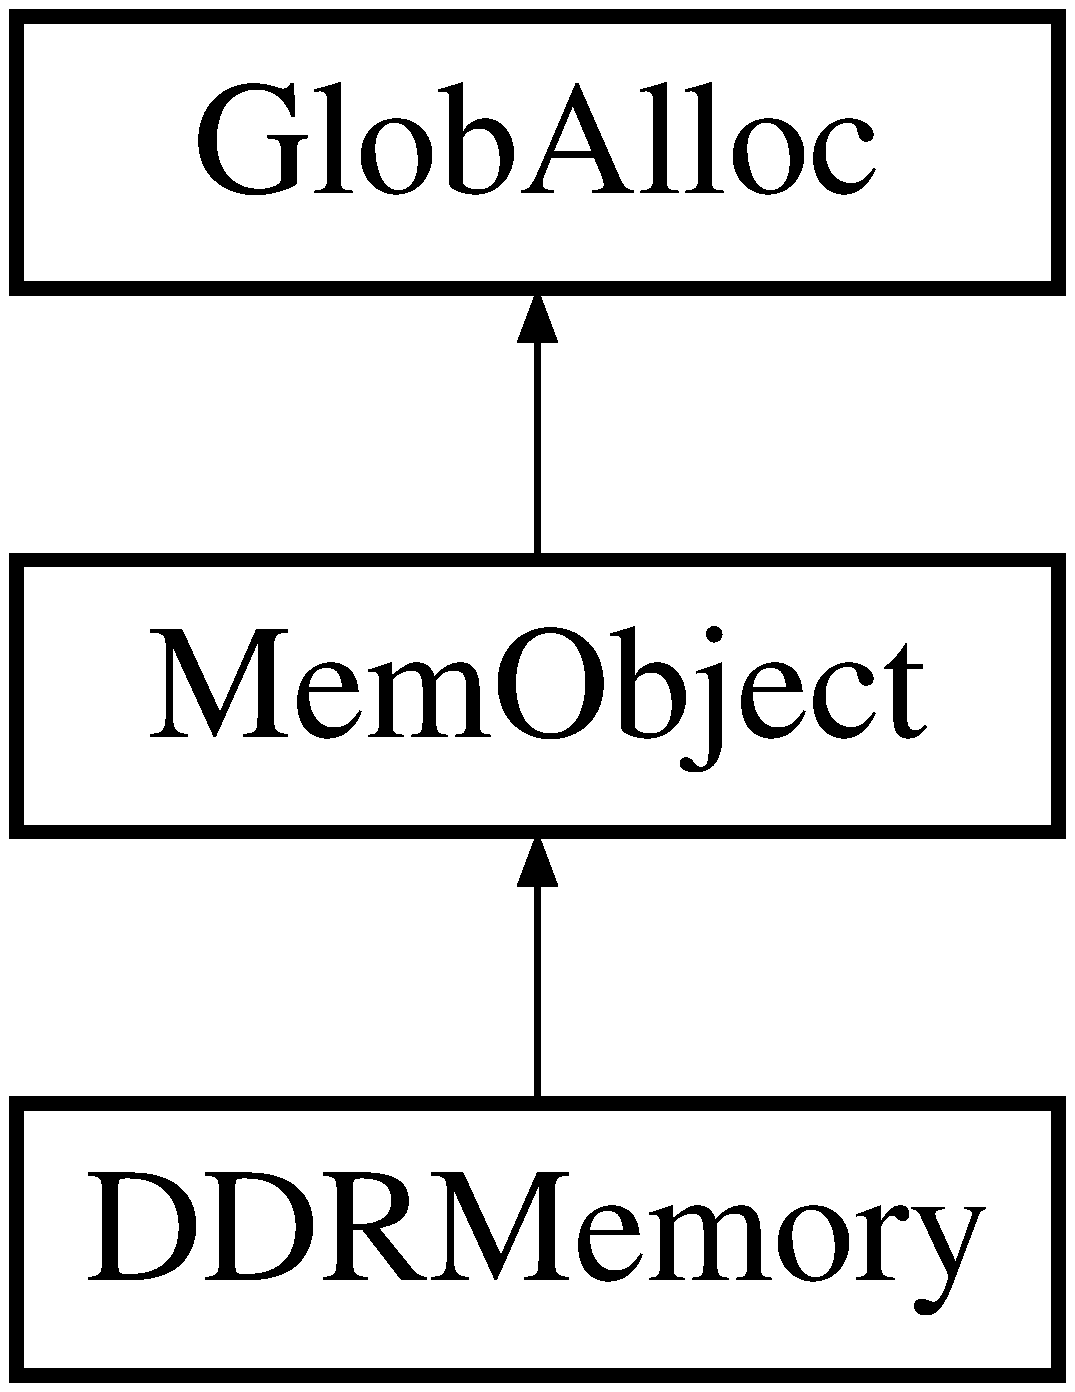
\includegraphics[height=3.000000cm]{classDDRMemory}
\end{center}
\end{figure}
\subsection*{Public Member Functions}
\begin{DoxyCompactItemize}
\item 
\hypertarget{classDDRMemory_aa395b8a32cf5406305897e0610522778}{{\bfseries D\-D\-R\-Memory} (uint32\-\_\-t \-\_\-line\-Size, uint32\-\_\-t \-\_\-col\-Size, uint32\-\_\-t \-\_\-ranks\-Per\-Channel, uint32\-\_\-t \-\_\-banks\-Per\-Rank, uint32\-\_\-t \-\_\-sys\-Freq\-M\-Hz, const char $\ast$tech, const char $\ast$addr\-Mapping, uint32\-\_\-t \-\_\-controller\-Sys\-Latency, uint32\-\_\-t \-\_\-queue\-Depth, uint32\-\_\-t \-\_\-row\-Hit\-Limit, bool \-\_\-deferred\-Writes, bool \-\_\-closed\-Page, uint32\-\_\-t \-\_\-domain, g\-\_\-string \&\-\_\-name, uint32\-\_\-t \-\_\-t\-B\-L=4, double time\-\_\-scale=1.\-0)}\label{classDDRMemory_aa395b8a32cf5406305897e0610522778}

\item 
\hypertarget{classDDRMemory_a58c0d5633d6ada4c71d06a452ca716a1}{void {\bfseries init\-Stats} (\hyperlink{classAggregateStat}{Aggregate\-Stat} $\ast$parent\-Stat)}\label{classDDRMemory_a58c0d5633d6ada4c71d06a452ca716a1}

\item 
\hypertarget{classDDRMemory_a0755b4e9f98c10e62c437ae7d7111c0a}{const char $\ast$ {\bfseries get\-Name} ()}\label{classDDRMemory_a0755b4e9f98c10e62c437ae7d7111c0a}

\item 
\hypertarget{classDDRMemory_a2f25f7e10c2687de33715398b71b2f3b}{uint64\-\_\-t {\bfseries access} (\hyperlink{structMemReq}{Mem\-Req} \&req, int type, uint32\-\_\-t data\-\_\-size=4)}\label{classDDRMemory_a2f25f7e10c2687de33715398b71b2f3b}

\item 
\hypertarget{classDDRMemory_a1bc441f6c27aa782f6c10ffcc44a74aa}{uint64\-\_\-t {\bfseries access} (\hyperlink{structMemReq}{Mem\-Req} \&req)}\label{classDDRMemory_a1bc441f6c27aa782f6c10ffcc44a74aa}

\item 
\hypertarget{classDDRMemory_a749d93a0a63f591c794c9718da692c8f}{void {\bfseries enqueue} (\hyperlink{classDDRMemoryAccEvent}{D\-D\-R\-Memory\-Acc\-Event} $\ast$ev, uint64\-\_\-t cycle)}\label{classDDRMemory_a749d93a0a63f591c794c9718da692c8f}

\item 
\hypertarget{classDDRMemory_a3f20a7e4a2d31a9220f3da4b39f84768}{void {\bfseries refresh} (uint64\-\_\-t sys\-Cycle)}\label{classDDRMemory_a3f20a7e4a2d31a9220f3da4b39f84768}

\item 
\hypertarget{classDDRMemory_a5ce560abc597aef55fa3f21b28d00d58}{uint64\-\_\-t {\bfseries tick} (uint64\-\_\-t sys\-Cycle)}\label{classDDRMemory_a5ce560abc597aef55fa3f21b28d00d58}

\item 
\hypertarget{classDDRMemory_a53c30add30e8bff9a8c8610ef449d86b}{void {\bfseries recycle\-Event} (\hyperlink{classSchedEvent}{Sched\-Event} $\ast$ev)}\label{classDDRMemory_a53c30add30e8bff9a8c8610ef449d86b}

\end{DoxyCompactItemize}


The documentation for this class was generated from the following files\-:\begin{DoxyCompactItemize}
\item 
ddr\-\_\-mem.\-h\item 
ddr\-\_\-mem.\-cpp\end{DoxyCompactItemize}

\hypertarget{classDDRMemoryAccEvent}{\section{D\-D\-R\-Memory\-Acc\-Event Class Reference}
\label{classDDRMemoryAccEvent}\index{D\-D\-R\-Memory\-Acc\-Event@{D\-D\-R\-Memory\-Acc\-Event}}
}
Inheritance diagram for D\-D\-R\-Memory\-Acc\-Event\-:\begin{figure}[H]
\begin{center}
\leavevmode
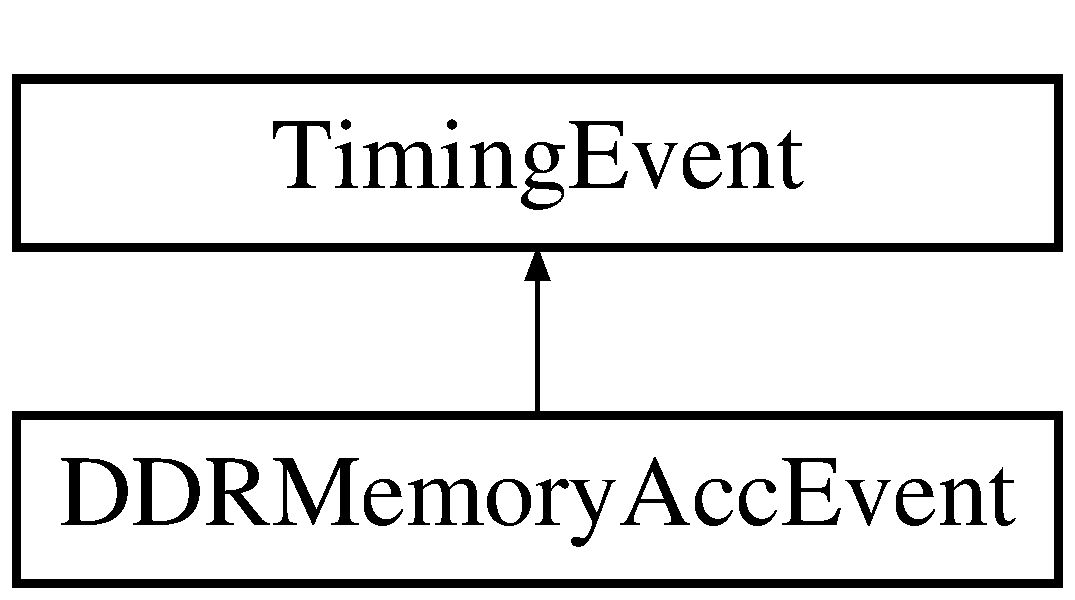
\includegraphics[height=2.000000cm]{classDDRMemoryAccEvent}
\end{center}
\end{figure}
\subsection*{Public Member Functions}
\begin{DoxyCompactItemize}
\item 
\hypertarget{classDDRMemoryAccEvent_a48e243a2b1d85590ff162a8bacb7fe06}{{\bfseries D\-D\-R\-Memory\-Acc\-Event} (\hyperlink{classDDRMemory}{D\-D\-R\-Memory} $\ast$\-\_\-mem, bool \-\_\-is\-Write, Address \-\_\-addr, uint32\-\_\-t \-\_\-data\-\_\-size, int32\-\_\-t domain, uint32\-\_\-t pre\-Delay, uint32\-\_\-t post\-Delay)}\label{classDDRMemoryAccEvent_a48e243a2b1d85590ff162a8bacb7fe06}

\item 
\hypertarget{classDDRMemoryAccEvent_a9027a4ac2269ed13a4d7413757603608}{Address {\bfseries get\-Addr} () const }\label{classDDRMemoryAccEvent_a9027a4ac2269ed13a4d7413757603608}

\item 
\hypertarget{classDDRMemoryAccEvent_a8599665610dfb9a19724f8286f97e4ca}{bool {\bfseries is\-Write} () const }\label{classDDRMemoryAccEvent_a8599665610dfb9a19724f8286f97e4ca}

\item 
\hypertarget{classDDRMemoryAccEvent_a2ac5b6b762f34a18f7d07463ffd072be}{uint32\-\_\-t {\bfseries get\-Data\-Size} () const }\label{classDDRMemoryAccEvent_a2ac5b6b762f34a18f7d07463ffd072be}

\item 
\hypertarget{classDDRMemoryAccEvent_ae37e788bac980a59b318cdabcf53e817}{void {\bfseries simulate} (uint64\-\_\-t start\-Cycle)}\label{classDDRMemoryAccEvent_ae37e788bac980a59b318cdabcf53e817}

\end{DoxyCompactItemize}
\subsection*{Additional Inherited Members}


The documentation for this class was generated from the following file\-:\begin{DoxyCompactItemize}
\item 
ddr\-\_\-mem.\-cpp\end{DoxyCompactItemize}

\hypertarget{classDecoder}{\section{Decoder Class Reference}
\label{classDecoder}\index{Decoder@{Decoder}}
}
\subsection*{Static Public Member Functions}
\begin{DoxyCompactItemize}
\item 
\hypertarget{classDecoder_a42cfea2d7b919c4be5a8406f4a298950}{static \hyperlink{structBblInfo}{Bbl\-Info} $\ast$ {\bfseries decode\-Bbl} (B\-B\-L bbl, bool ooo\-Decoding)}\label{classDecoder_a42cfea2d7b919c4be5a8406f4a298950}

\end{DoxyCompactItemize}


The documentation for this class was generated from the following files\-:\begin{DoxyCompactItemize}
\item 
decoder.\-h\item 
decoder.\-cpp\end{DoxyCompactItemize}

\hypertarget{classDelayEvent}{\section{Delay\-Event Class Reference}
\label{classDelayEvent}\index{Delay\-Event@{Delay\-Event}}
}
Inheritance diagram for Delay\-Event\-:\begin{figure}[H]
\begin{center}
\leavevmode
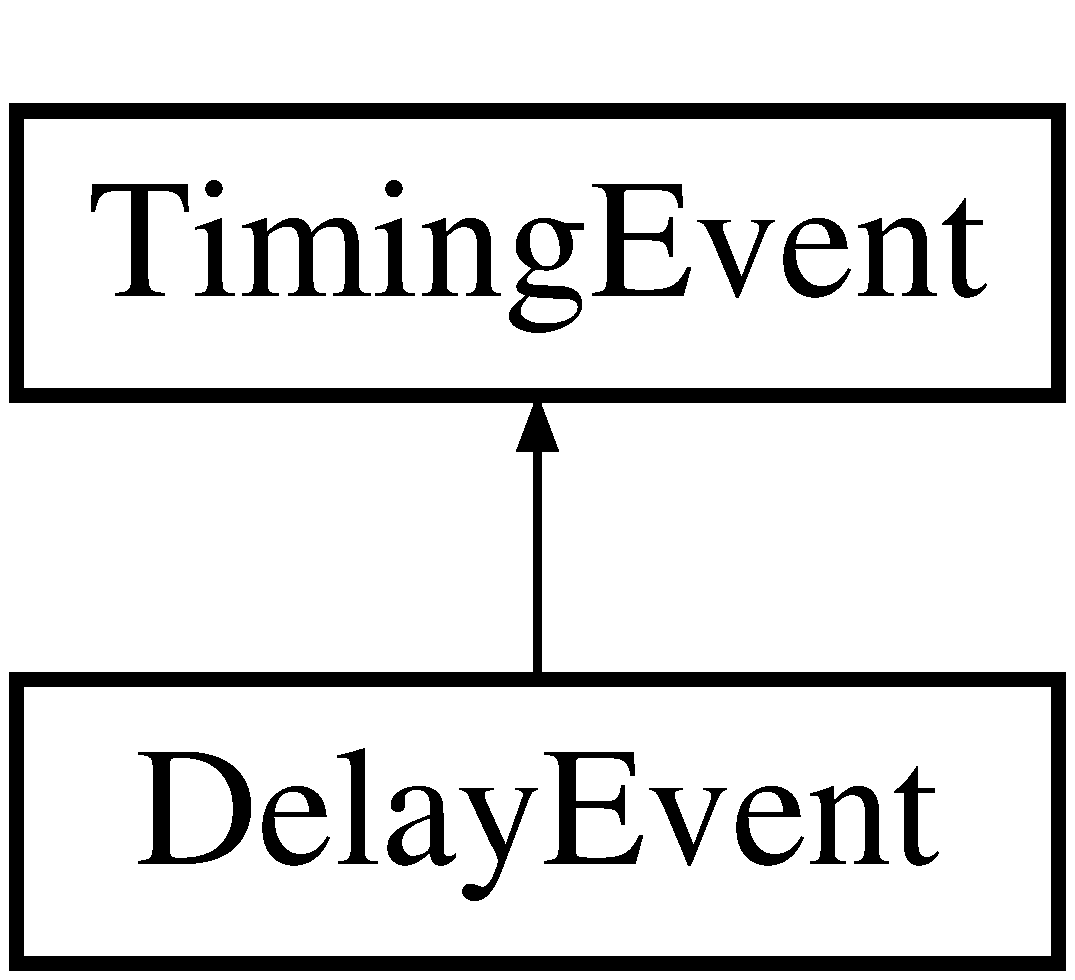
\includegraphics[height=2.000000cm]{classDelayEvent}
\end{center}
\end{figure}
\subsection*{Public Member Functions}
\begin{DoxyCompactItemize}
\item 
\hypertarget{classDelayEvent_a32bb27c084add7841c78f901efe2f74d}{{\bfseries Delay\-Event} (uint32\-\_\-t delay)}\label{classDelayEvent_a32bb27c084add7841c78f901efe2f74d}

\item 
virtual void \hyperlink{classDelayEvent_aa1a9ef6d5dc0d8c74f6e2c52d217ef73}{parent\-Done} (uint64\-\_\-t start\-Cycle)
\item 
\hypertarget{classDelayEvent_a9c9f03ccb0199158ed88836b618b6359}{virtual void {\bfseries simulate} (uint64\-\_\-t sim\-Cycle)}\label{classDelayEvent_a9c9f03ccb0199158ed88836b618b6359}

\end{DoxyCompactItemize}
\subsection*{Additional Inherited Members}


\subsection{Member Function Documentation}
\hypertarget{classDelayEvent_aa1a9ef6d5dc0d8c74f6e2c52d217ef73}{\index{Delay\-Event@{Delay\-Event}!parent\-Done@{parent\-Done}}
\index{parent\-Done@{parent\-Done}!DelayEvent@{Delay\-Event}}
\subsubsection[{parent\-Done}]{\setlength{\rightskip}{0pt plus 5cm}virtual void Delay\-Event\-::parent\-Done (
\begin{DoxyParamCaption}
\item[{uint64\-\_\-t}]{start\-Cycle}
\end{DoxyParamCaption}
)\hspace{0.3cm}{\ttfamily [inline]}, {\ttfamily [virtual]}}}\label{classDelayEvent_aa1a9ef6d5dc0d8c74f6e2c52d217ef73}
\$lic\$ Copyright (C) 2012-\/2015 by Massachusetts Institute of Technology Copyright (C) 2010-\/2013 by The Board of Trustees of Stanford University

This file is part of zsim.

zsim is free software; you can redistribute it and/or modify it under the terms of the G\-N\-U General Public License as published by the Free Software Foundation, version 2.

If you use this software in your research, we request that you reference the zsim paper (\char`\"{}\-Z\-Sim\-: Fast and Accurate Microarchitectural Simulation of
\-Thousand-\/\-Core Systems\char`\"{}, Sanchez and Kozyrakis, I\-S\-C\-A-\/40, June 2013) as the source of the simulator in any publications that use this software, and that you send us a citation of your work.

zsim is distributed in the hope that it will be useful, but W\-I\-T\-H\-O\-U\-T A\-N\-Y W\-A\-R\-R\-A\-N\-T\-Y; without even the implied warranty of M\-E\-R\-C\-H\-A\-N\-T\-A\-B\-I\-L\-I\-T\-Y or F\-I\-T\-N\-E\-S\-S F\-O\-R A P\-A\-R\-T\-I\-C\-U\-L\-A\-R P\-U\-R\-P\-O\-S\-E. See the G\-N\-U General Public License for more details.

You should have received a copy of the G\-N\-U General Public License along with this program. If not, see \href{http://www.gnu.org/licenses/}{\tt http\-://www.\-gnu.\-org/licenses/}. 

Reimplemented from \hyperlink{classTimingEvent_a55e7e2942d6607eb2a9dd484baf39070}{Timing\-Event}.



The documentation for this class was generated from the following file\-:\begin{DoxyCompactItemize}
\item 
timing\-\_\-event.\-h\end{DoxyCompactItemize}

\hypertarget{classDRAMSimMemory}{\section{D\-R\-A\-M\-Sim\-Memory Class Reference}
\label{classDRAMSimMemory}\index{D\-R\-A\-M\-Sim\-Memory@{D\-R\-A\-M\-Sim\-Memory}}
}
Inheritance diagram for D\-R\-A\-M\-Sim\-Memory\-:\begin{figure}[H]
\begin{center}
\leavevmode
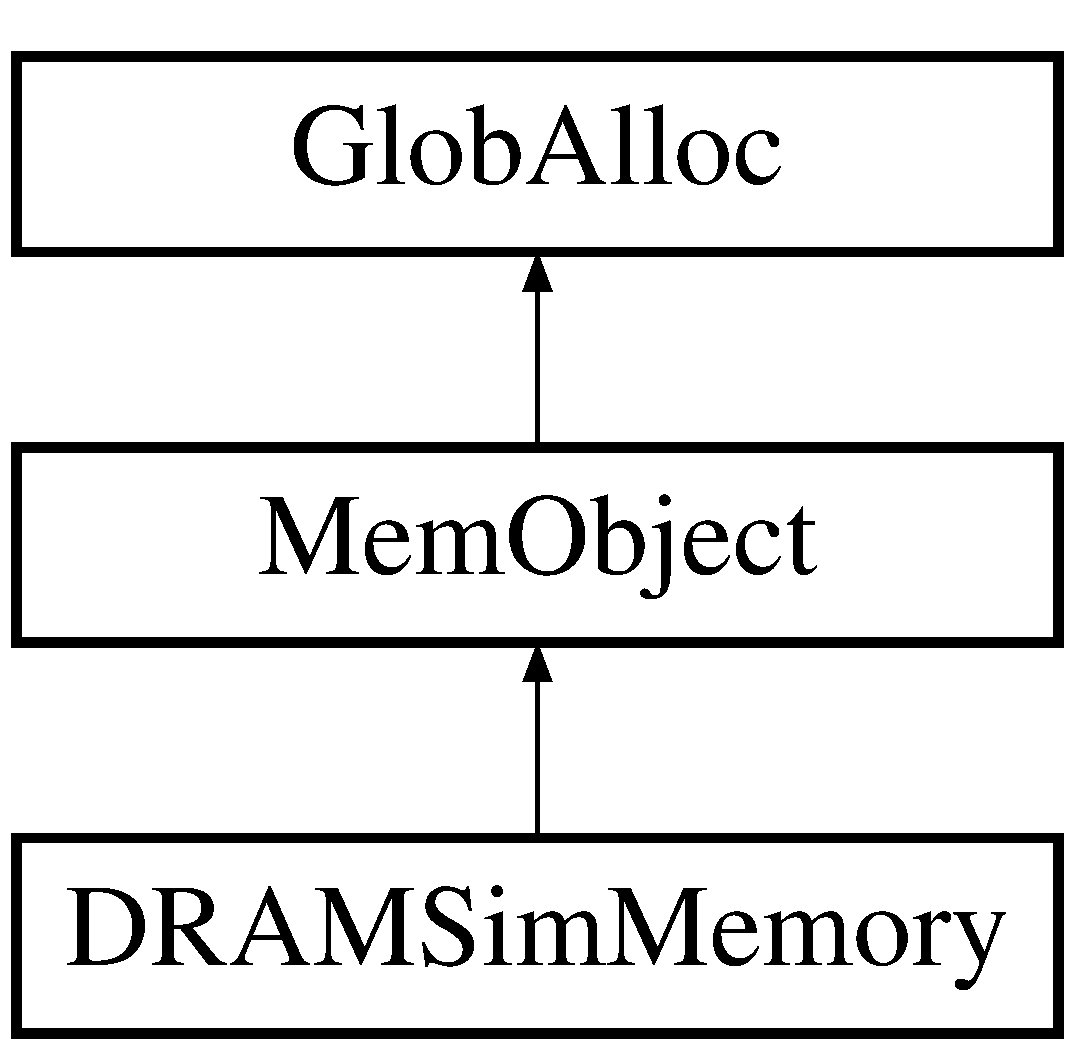
\includegraphics[height=3.000000cm]{classDRAMSimMemory}
\end{center}
\end{figure}
\subsection*{Public Member Functions}
\begin{DoxyCompactItemize}
\item 
\hypertarget{classDRAMSimMemory_a62c51e3bd12940fd4ab74a8d5b8de1ed}{{\bfseries D\-R\-A\-M\-Sim\-Memory} (std\-::string \&dram\-Tech\-Ini, std\-::string \&dram\-System\-Ini, std\-::string \&output\-Dir, std\-::string \&trace\-Name, uint32\-\_\-t capacity\-M\-B, uint64\-\_\-t cpu\-Freq\-Hz, uint32\-\_\-t \-\_\-min\-Latency, uint32\-\_\-t \-\_\-domain, const g\-\_\-string \&\-\_\-name)}\label{classDRAMSimMemory_a62c51e3bd12940fd4ab74a8d5b8de1ed}

\item 
\hypertarget{classDRAMSimMemory_a712837b00ca1ff452c6b314d0eac70ec}{const char $\ast$ {\bfseries get\-Name} ()}\label{classDRAMSimMemory_a712837b00ca1ff452c6b314d0eac70ec}

\item 
\hypertarget{classDRAMSimMemory_a270e07a2c22746179abb8d1e0ae442f6}{void {\bfseries init\-Stats} (\hyperlink{classAggregateStat}{Aggregate\-Stat} $\ast$parent\-Stat)}\label{classDRAMSimMemory_a270e07a2c22746179abb8d1e0ae442f6}

\item 
\hypertarget{classDRAMSimMemory_a0360046055a613f6fcf21abe76d68ac6}{uint64\-\_\-t {\bfseries access} (\hyperlink{structMemReq}{Mem\-Req} \&req, int type, uint32\-\_\-t data\-\_\-size=4)}\label{classDRAMSimMemory_a0360046055a613f6fcf21abe76d68ac6}

\item 
\hypertarget{classDRAMSimMemory_aec4b3a71bfa1e021e34d6091c31ffb97}{uint64\-\_\-t {\bfseries access} (\hyperlink{structMemReq}{Mem\-Req} \&req)}\label{classDRAMSimMemory_aec4b3a71bfa1e021e34d6091c31ffb97}

\item 
\hypertarget{classDRAMSimMemory_ae3e9517bb81acd6cc17961f210490db5}{uint32\-\_\-t {\bfseries tick} (uint64\-\_\-t cycle)}\label{classDRAMSimMemory_ae3e9517bb81acd6cc17961f210490db5}

\item 
\hypertarget{classDRAMSimMemory_a71ba63111322818f232cd1efc04a5aff}{void {\bfseries enqueue} (D\-R\-A\-M\-Sim\-Acc\-Event $\ast$ev, uint64\-\_\-t cycle)}\label{classDRAMSimMemory_a71ba63111322818f232cd1efc04a5aff}

\end{DoxyCompactItemize}


The documentation for this class was generated from the following files\-:\begin{DoxyCompactItemize}
\item 
dramsim\-\_\-mem\-\_\-ctrl.\-h\item 
dramsim\-\_\-mem\-\_\-ctrl.\-cpp\end{DoxyCompactItemize}

\hypertarget{structDynBbl}{\section{Dyn\-Bbl Struct Reference}
\label{structDynBbl}\index{Dyn\-Bbl@{Dyn\-Bbl}}
}
\subsection*{Public Member Functions}
\begin{DoxyCompactItemize}
\item 
\hypertarget{structDynBbl_aa2a47443851deb46b1e6cb8005fb5c73}{void {\bfseries init} (uint64\-\_\-t \-\_\-addr, uint32\-\_\-t \-\_\-uops, uint32\-\_\-t \-\_\-approx\-Instrs)}\label{structDynBbl_aa2a47443851deb46b1e6cb8005fb5c73}

\end{DoxyCompactItemize}
\subsection*{Static Public Member Functions}
\begin{DoxyCompactItemize}
\item 
\hypertarget{structDynBbl_abb2c7976dbf8ee0f787eb153273172ad}{static uint32\-\_\-t {\bfseries bytes} (uint32\-\_\-t uops)}\label{structDynBbl_abb2c7976dbf8ee0f787eb153273172ad}

\end{DoxyCompactItemize}
\subsection*{Public Attributes}
\begin{DoxyCompactItemize}
\item 
\hypertarget{structDynBbl_abb71dd4e4dbdc3178f94b3d5b2742aab}{uint64\-\_\-t {\bfseries addr}}\label{structDynBbl_abb71dd4e4dbdc3178f94b3d5b2742aab}

\item 
\hypertarget{structDynBbl_a3f765e60798a5498d73f43a72984ecc8}{uint32\-\_\-t {\bfseries uops}}\label{structDynBbl_a3f765e60798a5498d73f43a72984ecc8}

\item 
\hypertarget{structDynBbl_a164ce491b4a0e15ed3f0a0ed9e23eb76}{uint32\-\_\-t {\bfseries approx\-Instrs}}\label{structDynBbl_a164ce491b4a0e15ed3f0a0ed9e23eb76}

\item 
\hypertarget{structDynBbl_a57bd9f35d60370524df19197235d8067}{\hyperlink{structDynUop}{Dyn\-Uop} {\bfseries uop} \mbox{[}1\mbox{]}}\label{structDynBbl_a57bd9f35d60370524df19197235d8067}

\end{DoxyCompactItemize}


The documentation for this struct was generated from the following file\-:\begin{DoxyCompactItemize}
\item 
decoder.\-h\end{DoxyCompactItemize}

\hypertarget{structDynUop}{\section{Dyn\-Uop Struct Reference}
\label{structDynUop}\index{Dyn\-Uop@{Dyn\-Uop}}
}
\subsection*{Public Member Functions}
\begin{DoxyCompactItemize}
\item 
\hypertarget{structDynUop_a96f4472cb4f8cc87716dee750e5892b6}{void {\bfseries clear} ()}\label{structDynUop_a96f4472cb4f8cc87716dee750e5892b6}

\end{DoxyCompactItemize}
\subsection*{Public Attributes}
\begin{DoxyCompactItemize}
\item 
\hypertarget{structDynUop_a1204f8a686324e3826eedf3315c69b31}{uint16\-\_\-t {\bfseries rs} \mbox{[}M\-A\-X\-\_\-\-U\-O\-P\-\_\-\-S\-R\-C\-\_\-\-R\-E\-G\-S\mbox{]}}\label{structDynUop_a1204f8a686324e3826eedf3315c69b31}

\item 
\hypertarget{structDynUop_a6ff81982a3a12efb287f8fa82b721b1a}{uint16\-\_\-t {\bfseries rd} \mbox{[}M\-A\-X\-\_\-\-U\-O\-P\-\_\-\-D\-S\-T\-\_\-\-R\-E\-G\-S\mbox{]}}\label{structDynUop_a6ff81982a3a12efb287f8fa82b721b1a}

\item 
\hypertarget{structDynUop_a8f4dd7055e58cce2acd4a21d7866f911}{uint16\-\_\-t {\bfseries lat}}\label{structDynUop_a8f4dd7055e58cce2acd4a21d7866f911}

\item 
\hypertarget{structDynUop_a51505d0954480a5b856a4b9342357f48}{uint16\-\_\-t {\bfseries dec\-Cycle}}\label{structDynUop_a51505d0954480a5b856a4b9342357f48}

\item 
\hypertarget{structDynUop_a5a309347ba3cd03722933cc76d602901}{Uop\-Type {\bfseries type}}\label{structDynUop_a5a309347ba3cd03722933cc76d602901}

\item 
\hypertarget{structDynUop_a70216f1b9716267522764b6bf87df694}{uint8\-\_\-t {\bfseries port\-Mask}}\label{structDynUop_a70216f1b9716267522764b6bf87df694}

\item 
\hypertarget{structDynUop_a34d22710b2f2a95b0012ca52d2b5676e}{uint8\-\_\-t {\bfseries extra\-Slots}}\label{structDynUop_a34d22710b2f2a95b0012ca52d2b5676e}

\item 
\hypertarget{structDynUop_ab46ee8d7a4e65c672e47a9c162704f76}{uint8\-\_\-t {\bfseries pad}}\label{structDynUop_ab46ee8d7a4e65c672e47a9c162704f76}

\end{DoxyCompactItemize}


The documentation for this struct was generated from the following files\-:\begin{DoxyCompactItemize}
\item 
decoder.\-h\item 
decoder.\-cpp\end{DoxyCompactItemize}

\hypertarget{structIdealLRUPartReplPolicy_1_1Entry}{\section{Ideal\-L\-R\-U\-Part\-Repl\-Policy\-:\-:Entry Struct Reference}
\label{structIdealLRUPartReplPolicy_1_1Entry}\index{Ideal\-L\-R\-U\-Part\-Repl\-Policy\-::\-Entry@{Ideal\-L\-R\-U\-Part\-Repl\-Policy\-::\-Entry}}
}
Inheritance diagram for Ideal\-L\-R\-U\-Part\-Repl\-Policy\-:\-:Entry\-:\begin{figure}[H]
\begin{center}
\leavevmode
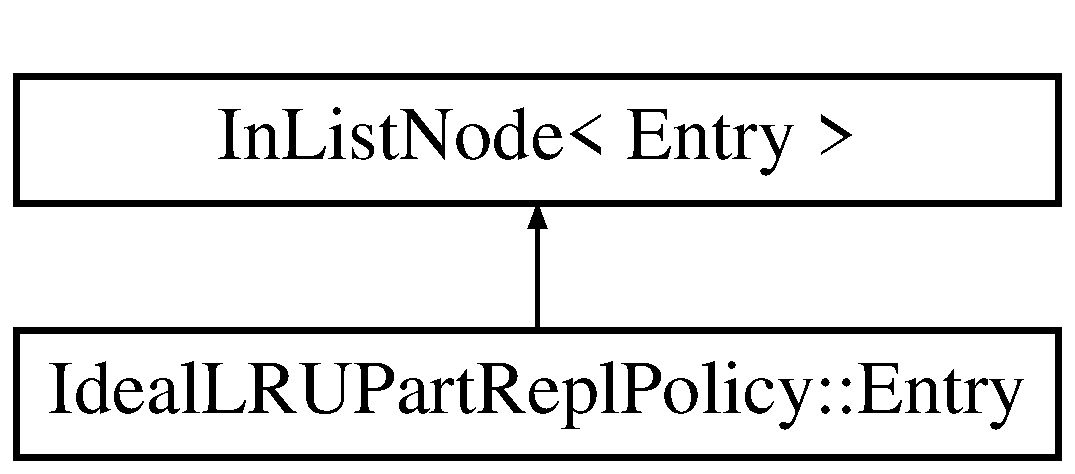
\includegraphics[height=2.000000cm]{structIdealLRUPartReplPolicy_1_1Entry}
\end{center}
\end{figure}
\subsection*{Public Member Functions}
\begin{DoxyCompactItemize}
\item 
\hypertarget{structIdealLRUPartReplPolicy_1_1Entry_a83695ad1156d89ac833e458d6a5ea06c}{{\bfseries Entry} (uint32\-\_\-t \-\_\-id, uint32\-\_\-t \-\_\-p)}\label{structIdealLRUPartReplPolicy_1_1Entry_a83695ad1156d89ac833e458d6a5ea06c}

\end{DoxyCompactItemize}
\subsection*{Public Attributes}
\begin{DoxyCompactItemize}
\item 
\hypertarget{structIdealLRUPartReplPolicy_1_1Entry_a1036b5b4211c71dec55fb44c7747627c}{const uint32\-\_\-t {\bfseries line\-Id}}\label{structIdealLRUPartReplPolicy_1_1Entry_a1036b5b4211c71dec55fb44c7747627c}

\item 
\hypertarget{structIdealLRUPartReplPolicy_1_1Entry_abce594ee5f688615813e2f4ef97edde3}{uint32\-\_\-t {\bfseries p}}\label{structIdealLRUPartReplPolicy_1_1Entry_abce594ee5f688615813e2f4ef97edde3}

\item 
\hypertarget{structIdealLRUPartReplPolicy_1_1Entry_a17a8f5416e0db77d26a96751bd14e01f}{bool {\bfseries used}}\label{structIdealLRUPartReplPolicy_1_1Entry_a17a8f5416e0db77d26a96751bd14e01f}

\end{DoxyCompactItemize}


The documentation for this struct was generated from the following file\-:\begin{DoxyCompactItemize}
\item 
ideal\-\_\-arrays.\-h\end{DoxyCompactItemize}

\hypertarget{classEvent}{\section{Event Class Reference}
\label{classEvent}\index{Event@{Event}}
}


{\ttfamily \#include $<$event\-\_\-queue.\-h$>$}

Inheritance diagram for Event\-:\begin{figure}[H]
\begin{center}
\leavevmode
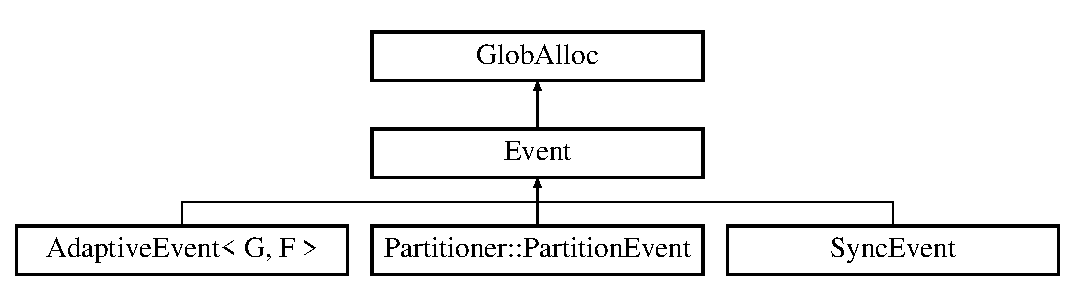
\includegraphics[height=3.000000cm]{classEvent}
\end{center}
\end{figure}
\subsection*{Public Member Functions}
\begin{DoxyCompactItemize}
\item 
\hypertarget{classEvent_a30314db1ee1d302e652b4fbdc6fd014f}{{\bfseries Event} (uint64\-\_\-t \-\_\-period)}\label{classEvent_a30314db1ee1d302e652b4fbdc6fd014f}

\item 
\hypertarget{classEvent_ab04472aa7d4a60a2c52edae3ed12cef2}{uint64\-\_\-t {\bfseries get\-Period} () const }\label{classEvent_ab04472aa7d4a60a2c52edae3ed12cef2}

\item 
\hypertarget{classEvent_a625651166eae427187cdc0c351a41315}{virtual void {\bfseries callback} ()=0}\label{classEvent_a625651166eae427187cdc0c351a41315}

\end{DoxyCompactItemize}
\subsection*{Protected Attributes}
\begin{DoxyCompactItemize}
\item 
\hypertarget{classEvent_a48c0276ea0ab0cc4043161bff53b145d}{uint64\-\_\-t {\bfseries period}}\label{classEvent_a48c0276ea0ab0cc4043161bff53b145d}

\end{DoxyCompactItemize}


\subsection{Detailed Description}
\$lic\$ Copyright (C) 2012-\/2015 by Massachusetts Institute of Technology Copyright (C) 2010-\/2013 by The Board of Trustees of Stanford University

This file is part of zsim.

zsim is free software; you can redistribute it and/or modify it under the terms of the G\-N\-U General Public License as published by the Free Software Foundation, version 2.

If you use this software in your research, we request that you reference the zsim paper (\char`\"{}\-Z\-Sim\-: Fast and Accurate Microarchitectural Simulation of
\-Thousand-\/\-Core Systems\char`\"{}, Sanchez and Kozyrakis, I\-S\-C\-A-\/40, June 2013) as the source of the simulator in any publications that use this software, and that you send us a citation of your work.

zsim is distributed in the hope that it will be useful, but W\-I\-T\-H\-O\-U\-T A\-N\-Y W\-A\-R\-R\-A\-N\-T\-Y; without even the implied warranty of M\-E\-R\-C\-H\-A\-N\-T\-A\-B\-I\-L\-I\-T\-Y or F\-I\-T\-N\-E\-S\-S F\-O\-R A P\-A\-R\-T\-I\-C\-U\-L\-A\-R P\-U\-R\-P\-O\-S\-E. See the G\-N\-U General Public License for more details.

You should have received a copy of the G\-N\-U General Public License along with this program. If not, see \href{http://www.gnu.org/licenses/}{\tt http\-://www.\-gnu.\-org/licenses/}. 

The documentation for this class was generated from the following file\-:\begin{DoxyCompactItemize}
\item 
event\-\_\-queue.\-h\end{DoxyCompactItemize}

\hypertarget{classEventQueue}{\section{Event\-Queue Class Reference}
\label{classEventQueue}\index{Event\-Queue@{Event\-Queue}}
}
Inheritance diagram for Event\-Queue\-:\begin{figure}[H]
\begin{center}
\leavevmode
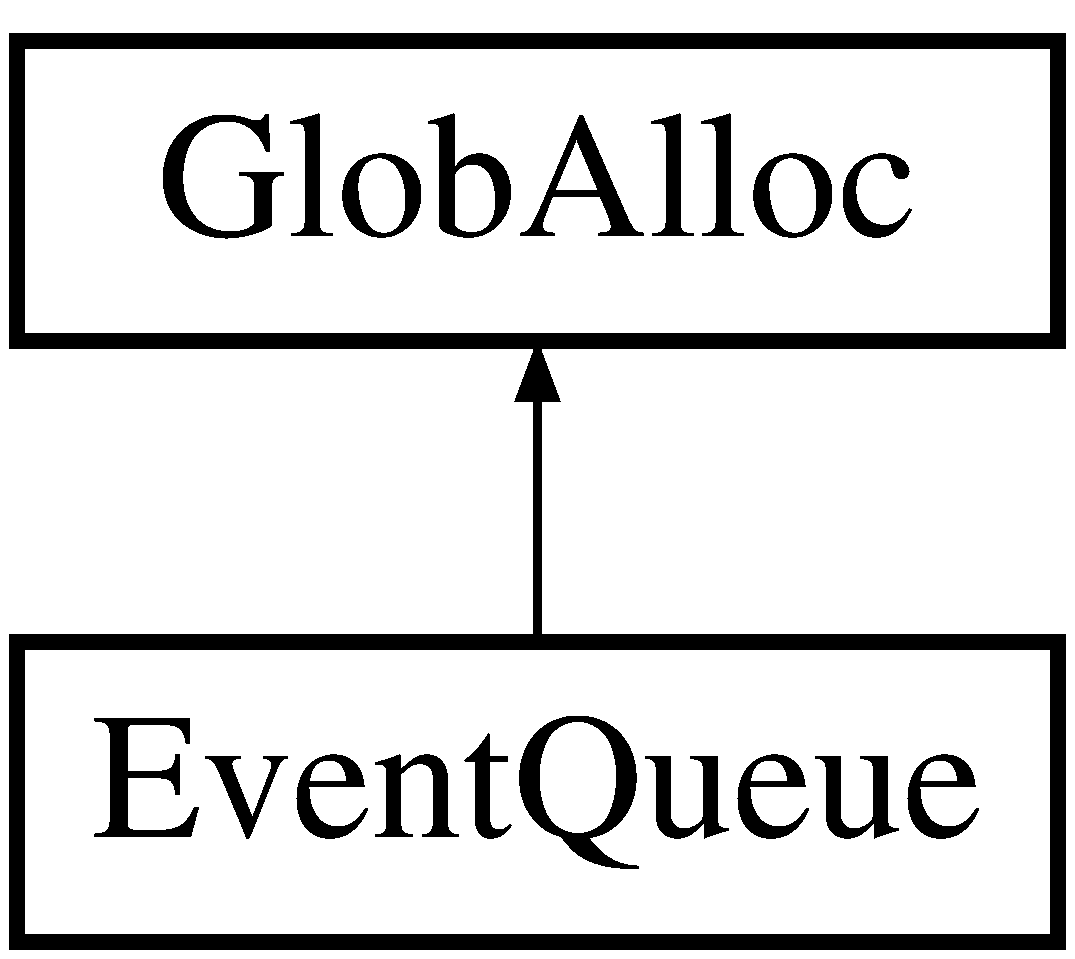
\includegraphics[height=2.000000cm]{classEventQueue}
\end{center}
\end{figure}
\subsection*{Public Member Functions}
\begin{DoxyCompactItemize}
\item 
\hypertarget{classEventQueue_afe0fdec3ed03ebe47b84e62b22842792}{void {\bfseries tick} ()}\label{classEventQueue_afe0fdec3ed03ebe47b84e62b22842792}

\item 
\hypertarget{classEventQueue_ab1d640e2257550aec21cc953fb524ac2}{void {\bfseries insert} (\hyperlink{classEvent}{Event} $\ast$ev, int64\-\_\-t start\-Delay=-\/1)}\label{classEventQueue_ab1d640e2257550aec21cc953fb524ac2}

\end{DoxyCompactItemize}


The documentation for this class was generated from the following file\-:\begin{DoxyCompactItemize}
\item 
event\-\_\-queue.\-h\end{DoxyCompactItemize}

\hypertarget{classEventRecorder}{\section{Event\-Recorder Class Reference}
\label{classEventRecorder}\index{Event\-Recorder@{Event\-Recorder}}
}
Inheritance diagram for Event\-Recorder\-:\begin{figure}[H]
\begin{center}
\leavevmode
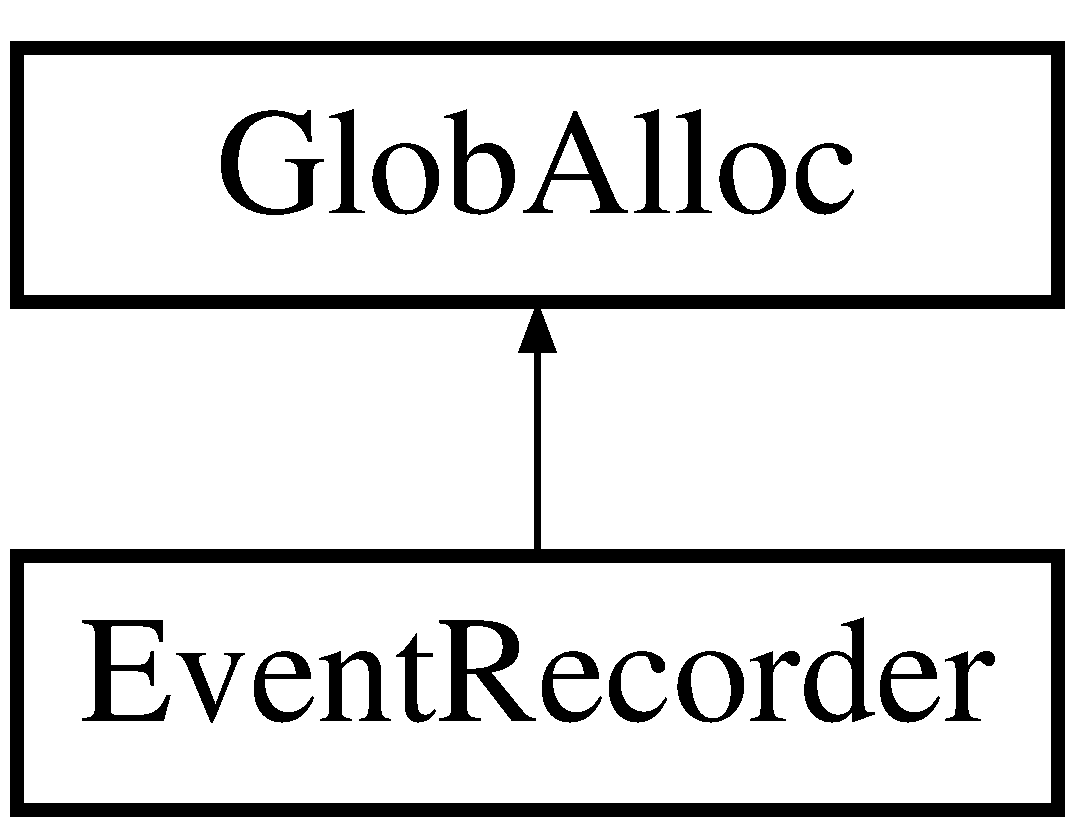
\includegraphics[height=2.000000cm]{classEventRecorder}
\end{center}
\end{figure}
\subsection*{Public Member Functions}
\begin{DoxyCompactItemize}
\item 
\hypertarget{classEventRecorder_a159f84907e26da94afefa727d0237305}{{\footnotesize template$<$typename T $>$ }\\T $\ast$ {\bfseries alloc} ()}\label{classEventRecorder_a159f84907e26da94afefa727d0237305}

\item 
\hypertarget{classEventRecorder_a41c38d3c5d52714385b52d276c2c1aa3}{void $\ast$ {\bfseries alloc} (size\-\_\-t sz)}\label{classEventRecorder_a41c38d3c5d52714385b52d276c2c1aa3}

\item 
\hypertarget{classEventRecorder_afc30252e62f21bc42a05eae12db00b70}{void {\bfseries push\-Record} (const \hyperlink{structTimingRecord}{Timing\-Record} \&rec)}\label{classEventRecorder_afc30252e62f21bc42a05eae12db00b70}

\item 
\hypertarget{classEventRecorder_a4a79087d8409e82b3b41fd2e4b5ecdef}{\hyperlink{structTimingRecord}{Timing\-Record} {\bfseries pop\-Record} () \-\_\-\-\_\-attribute\-\_\-\-\_\-((always\-\_\-inline))}\label{classEventRecorder_a4a79087d8409e82b3b41fd2e4b5ecdef}

\item 
\hypertarget{classEventRecorder_a335b5de4de0e0144d7829f8c75279f32}{size\-\_\-t {\bfseries has\-Record} () const }\label{classEventRecorder_a335b5de4de0e0144d7829f8c75279f32}

\item 
\hypertarget{classEventRecorder_a40ad92b26f50d5bae3daabe6c9485d19}{uint64\-\_\-t {\bfseries get\-Slack} (uint64\-\_\-t orig\-Start\-Cycle) const }\label{classEventRecorder_a40ad92b26f50d5bae3daabe6c9485d19}

\item 
\hypertarget{classEventRecorder_a49733c855c908748a220eaa61371bf8b}{uint64\-\_\-t {\bfseries get\-Gap\-Cycles} () const }\label{classEventRecorder_a49733c855c908748a220eaa61371bf8b}

\item 
\hypertarget{classEventRecorder_a738bacb75d4ae584eb44fa9dcba6ee7a}{void {\bfseries set\-Gap\-Cycles} (uint64\-\_\-t gap\-Cycles)}\label{classEventRecorder_a738bacb75d4ae584eb44fa9dcba6ee7a}

\item 
\hypertarget{classEventRecorder_a4a5078b32b484226d921538054fee4e8}{void {\bfseries set\-Start\-Slack} (uint64\-\_\-t start\-Slack)}\label{classEventRecorder_a4a5078b32b484226d921538054fee4e8}

\item 
\hypertarget{classEventRecorder_a825338b237bcd7ae9f7f65477a489a6f}{uint32\-\_\-t {\bfseries get\-Source\-Id} () const }\label{classEventRecorder_a825338b237bcd7ae9f7f65477a489a6f}

\item 
\hypertarget{classEventRecorder_a9c079787b3c2284d1defde04be45446f}{void {\bfseries set\-Source\-Id} (uint32\-\_\-t i)}\label{classEventRecorder_a9c079787b3c2284d1defde04be45446f}

\item 
\hypertarget{classEventRecorder_a37ec484c1773fbbb837c0ed5cf37acab}{\hyperlink{classg__vector}{Crossing\-Stack} \& {\bfseries get\-Crossing\-Stack} ()}\label{classEventRecorder_a37ec484c1773fbbb837c0ed5cf37acab}

\end{DoxyCompactItemize}


The documentation for this class was generated from the following file\-:\begin{DoxyCompactItemize}
\item 
event\-\_\-recorder.\-h\end{DoxyCompactItemize}

\hypertarget{classFilterCache}{\section{Filter\-Cache Class Reference}
\label{classFilterCache}\index{Filter\-Cache@{Filter\-Cache}}
}


{\ttfamily \#include $<$filter\-\_\-cache.\-h$>$}

Inheritance diagram for Filter\-Cache\-:\begin{figure}[H]
\begin{center}
\leavevmode
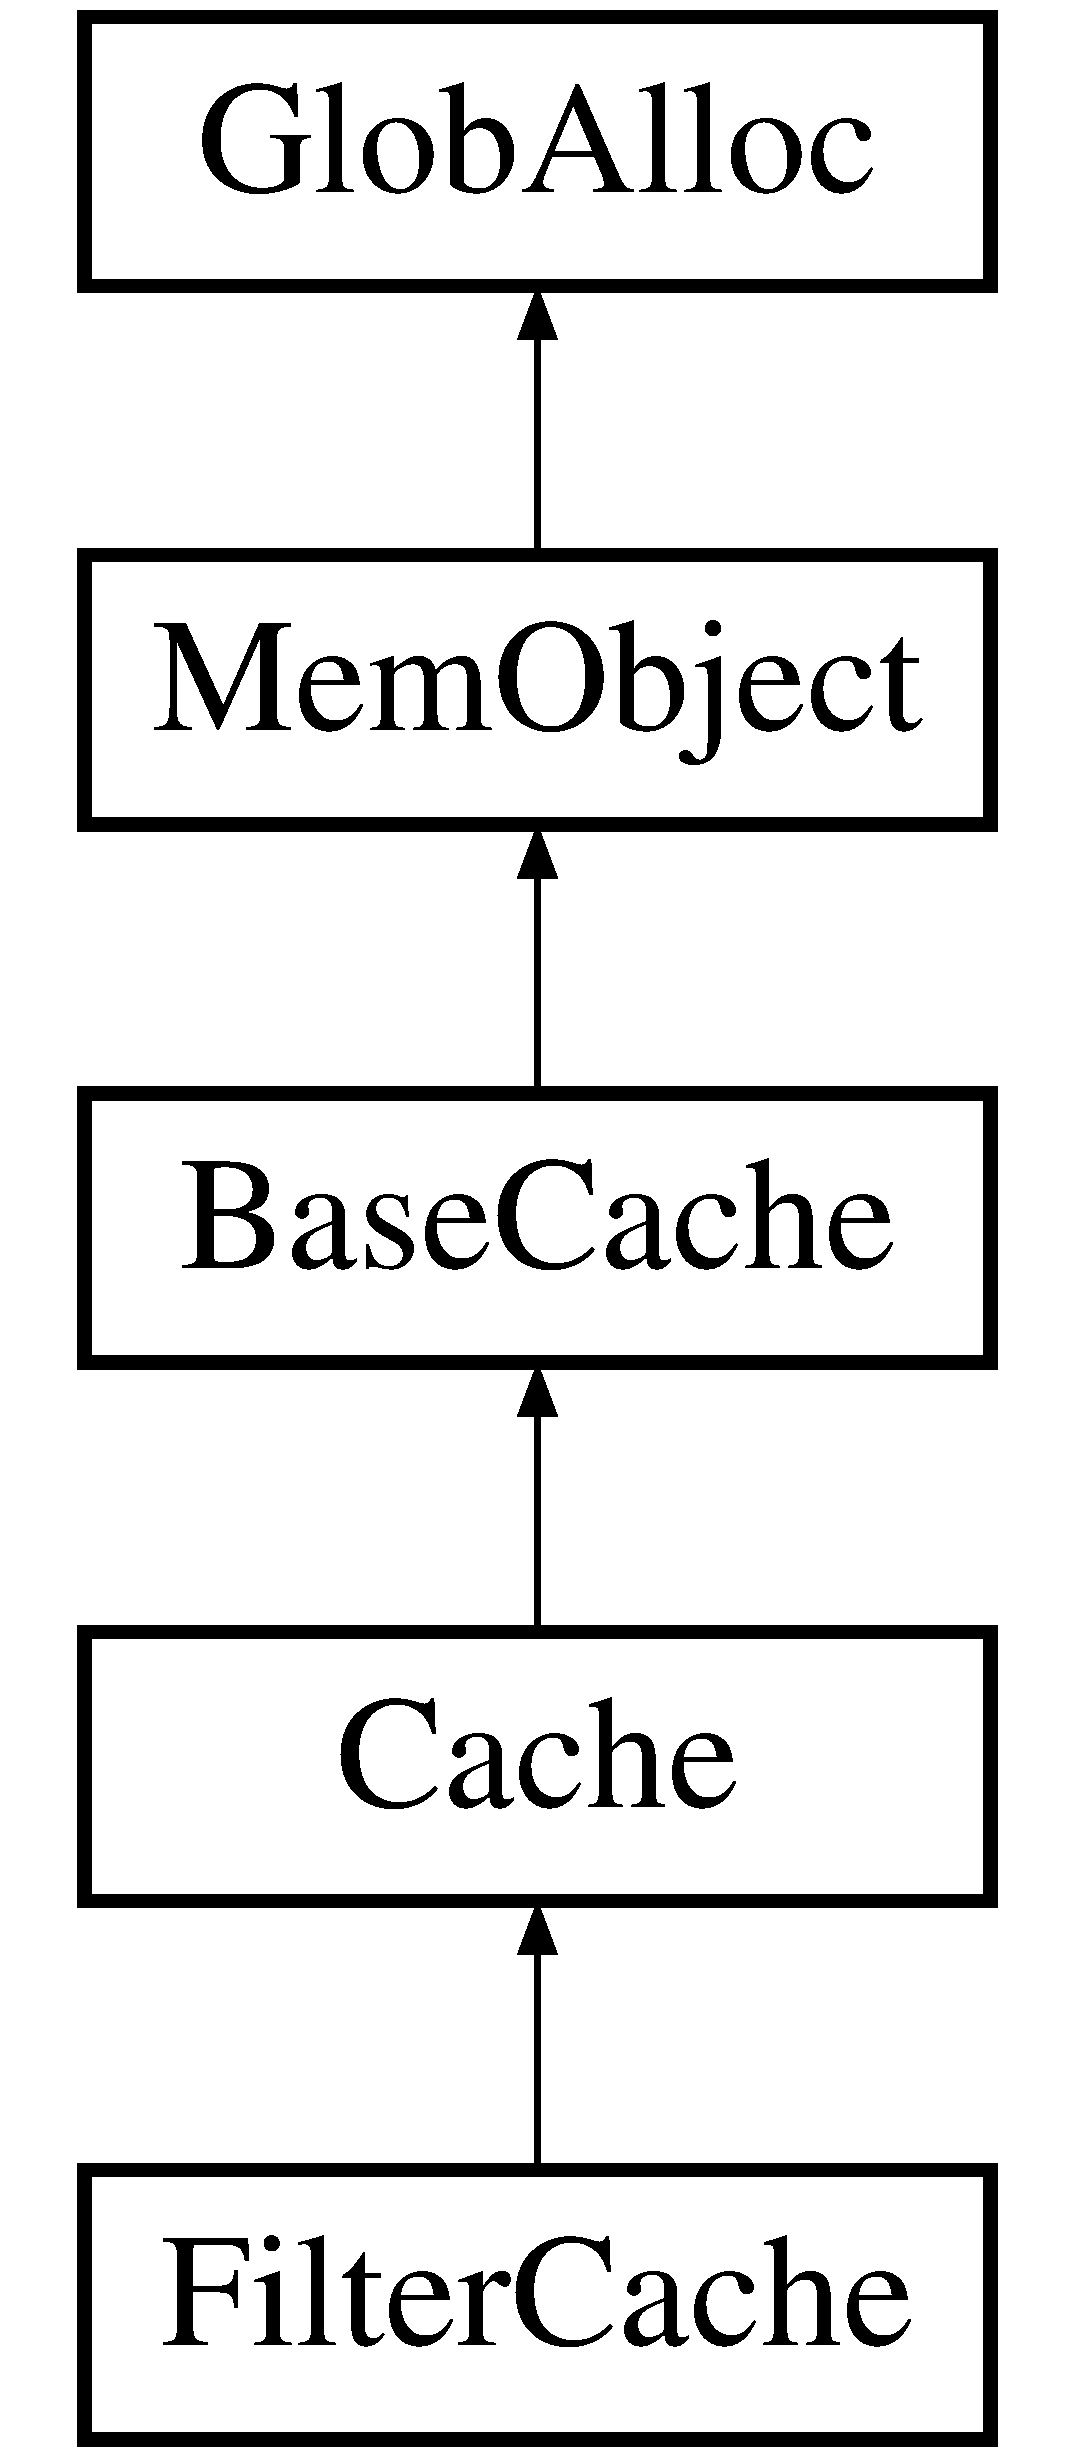
\includegraphics[height=5.000000cm]{classFilterCache}
\end{center}
\end{figure}
\subsection*{Public Member Functions}
\begin{DoxyCompactItemize}
\item 
\hypertarget{classFilterCache_a309ef8fa21b08e740d71df61fdcb5768}{{\bfseries Filter\-Cache} (uint32\-\_\-t \-\_\-num\-Sets, uint32\-\_\-t \-\_\-num\-Lines, \hyperlink{classCC}{C\-C} $\ast$\-\_\-cc, \hyperlink{classCacheArray}{Cache\-Array} $\ast$\-\_\-array, \hyperlink{classReplPolicy}{Repl\-Policy} $\ast$\-\_\-rp, uint32\-\_\-t \-\_\-acc\-Lat, uint32\-\_\-t \-\_\-inv\-Lat, g\-\_\-string \&\-\_\-name, \hyperlink{classConfig}{Config} \&config)}\label{classFilterCache_a309ef8fa21b08e740d71df61fdcb5768}

\item 
\hypertarget{classFilterCache_ade026c14eeb800335f9648563da9f6ed}{void {\bfseries set\-Source\-Id} (uint32\-\_\-t id)}\label{classFilterCache_ade026c14eeb800335f9648563da9f6ed}

\item 
\hypertarget{classFilterCache_a31a9f6cfc6b1e0374d1ddc104677a922}{void {\bfseries set\-Flags} (uint32\-\_\-t flags)}\label{classFilterCache_a31a9f6cfc6b1e0374d1ddc104677a922}

\item 
\hypertarget{classFilterCache_a8da6656008a754aad50e3784a2d7a667}{void {\bfseries init\-Stats} (\hyperlink{classAggregateStat}{Aggregate\-Stat} $\ast$parent\-Stat)}\label{classFilterCache_a8da6656008a754aad50e3784a2d7a667}

\item 
\hypertarget{classFilterCache_a1bd3192311a095740da165e296e0bb80}{uint64\-\_\-t {\bfseries load} (Address v\-Addr, uint64\-\_\-t cur\-Cycle)}\label{classFilterCache_a1bd3192311a095740da165e296e0bb80}

\item 
\hypertarget{classFilterCache_a919b949716858aafa3f2942c84aa4212}{uint64\-\_\-t {\bfseries store} (Address v\-Addr, uint64\-\_\-t cur\-Cycle)}\label{classFilterCache_a919b949716858aafa3f2942c84aa4212}

\item 
\hypertarget{classFilterCache_acedfa30e1ab154f2eac586cadc1dd96b}{uint64\-\_\-t {\bfseries replace} (Address v\-Line\-Addr, uint32\-\_\-t idx, bool is\-Load, uint64\-\_\-t cur\-Cycle)}\label{classFilterCache_acedfa30e1ab154f2eac586cadc1dd96b}

\item 
\hypertarget{classFilterCache_abbcca6a956003c482303421aa0638da1}{uint64\-\_\-t {\bfseries invalidate} (const \hyperlink{structInvReq}{Inv\-Req} \&req)}\label{classFilterCache_abbcca6a956003c482303421aa0638da1}

\item 
\hypertarget{classFilterCache_a2ad2ace77694d58bb47cf298963c6cd9}{void {\bfseries context\-Switch} ()}\label{classFilterCache_a2ad2ace77694d58bb47cf298963c6cd9}

\end{DoxyCompactItemize}
\subsection*{Additional Inherited Members}


\subsection{Detailed Description}
\$lic\$ Copyright (C) 2012-\/2015 by Massachusetts Institute of Technology Copyright (C) 2010-\/2013 by The Board of Trustees of Stanford University

This file is part of zsim.

zsim is free software; you can redistribute it and/or modify it under the terms of the G\-N\-U General Public License as published by the Free Software Foundation, version 2.

If you use this software in your research, we request that you reference the zsim paper (\char`\"{}\-Z\-Sim\-: Fast and Accurate Microarchitectural Simulation of
\-Thousand-\/\-Core Systems\char`\"{}, Sanchez and Kozyrakis, I\-S\-C\-A-\/40, June 2013) as the source of the simulator in any publications that use this software, and that you send us a citation of your work.

zsim is distributed in the hope that it will be useful, but W\-I\-T\-H\-O\-U\-T A\-N\-Y W\-A\-R\-R\-A\-N\-T\-Y; without even the implied warranty of M\-E\-R\-C\-H\-A\-N\-T\-A\-B\-I\-L\-I\-T\-Y or F\-I\-T\-N\-E\-S\-S F\-O\-R A P\-A\-R\-T\-I\-C\-U\-L\-A\-R P\-U\-R\-P\-O\-S\-E. See the G\-N\-U General Public License for more details.

You should have received a copy of the G\-N\-U General Public License along with this program. If not, see \href{http://www.gnu.org/licenses/}{\tt http\-://www.\-gnu.\-org/licenses/}. 

The documentation for this class was generated from the following file\-:\begin{DoxyCompactItemize}
\item 
filter\-\_\-cache.\-h\end{DoxyCompactItemize}

\hypertarget{classg__vector}{\section{g\-\_\-vector$<$ T $>$ Class Template Reference}
\label{classg__vector}\index{g\-\_\-vector$<$ T $>$@{g\-\_\-vector$<$ T $>$}}
}


The documentation for this class was generated from the following file\-:\begin{DoxyCompactItemize}
\item 
zsim.\-h\end{DoxyCompactItemize}

\hypertarget{classGlobAlloc}{\section{Glob\-Alloc Class Reference}
\label{classGlobAlloc}\index{Glob\-Alloc@{Glob\-Alloc}}
}
Inheritance diagram for Glob\-Alloc\-:\begin{figure}[H]
\begin{center}
\leavevmode
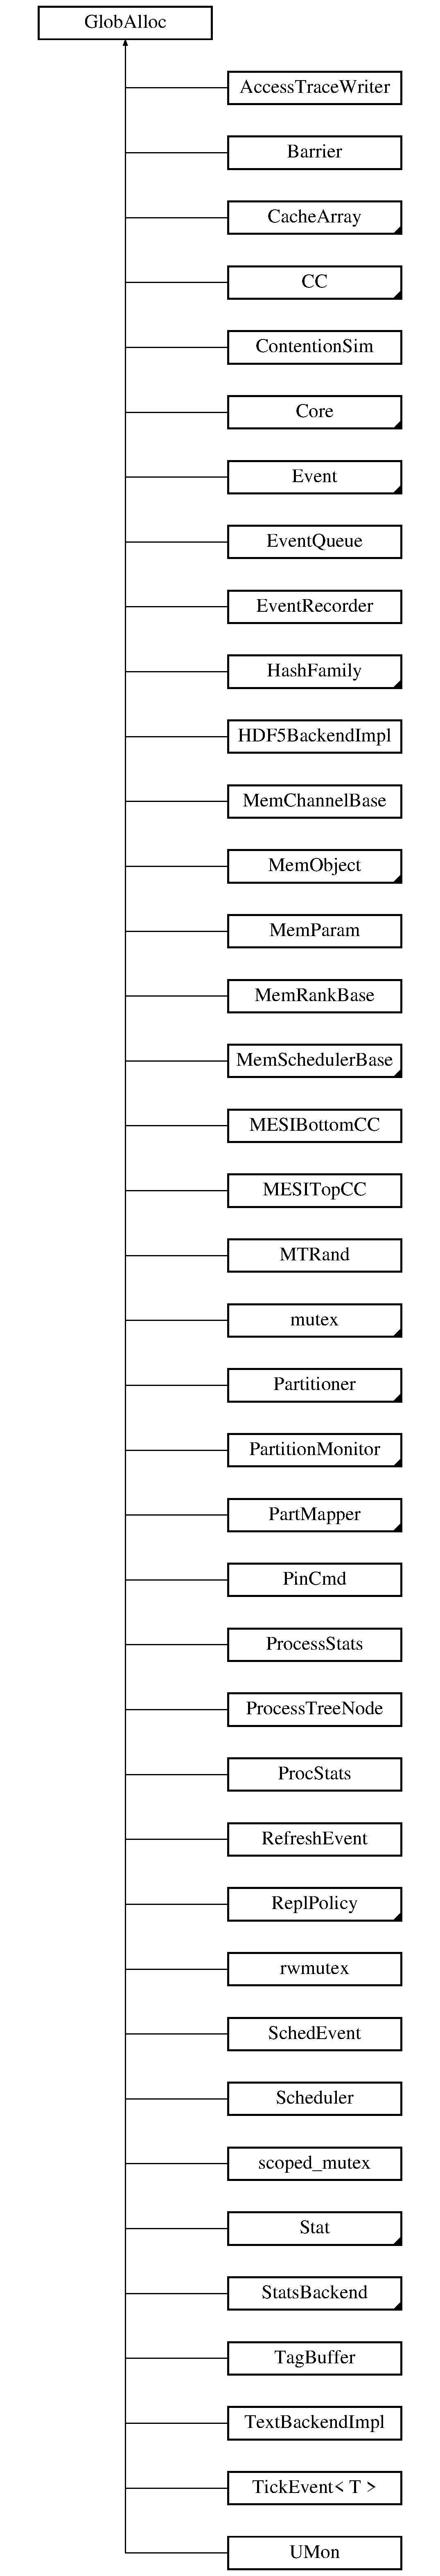
\includegraphics[height=12.000000cm]{classGlobAlloc}
\end{center}
\end{figure}
\subsection*{Public Member Functions}
\begin{DoxyCompactItemize}
\item 
\hypertarget{classGlobAlloc_acb2be4eaf93b490cf8c419aeccb53cee}{void $\ast$ {\bfseries operator new} (size\-\_\-t sz)}\label{classGlobAlloc_acb2be4eaf93b490cf8c419aeccb53cee}

\item 
\hypertarget{classGlobAlloc_ac16473b410af2b03d37dbdc97e43e629}{void $\ast$ {\bfseries operator new} (size\-\_\-t sz, void $\ast$ptr)}\label{classGlobAlloc_ac16473b410af2b03d37dbdc97e43e629}

\item 
\hypertarget{classGlobAlloc_aabc8fd6722597a3cfe37cf36352e304c}{void {\bfseries operator delete} (void $\ast$p, size\-\_\-t sz)}\label{classGlobAlloc_aabc8fd6722597a3cfe37cf36352e304c}

\item 
\hypertarget{classGlobAlloc_a53bb1bf97b9034b956963fae5b710d3a}{void {\bfseries operator delete} (void $\ast$p, void $\ast$ptr)}\label{classGlobAlloc_a53bb1bf97b9034b956963fae5b710d3a}

\end{DoxyCompactItemize}


The documentation for this class was generated from the following file\-:\begin{DoxyCompactItemize}
\item 
galloc.\-h\end{DoxyCompactItemize}

\hypertarget{structGlobSimInfo}{\section{Glob\-Sim\-Info Struct Reference}
\label{structGlobSimInfo}\index{Glob\-Sim\-Info@{Glob\-Sim\-Info}}
}
\subsection*{Public Member Functions}
\begin{DoxyCompactItemize}
\item 
\hypertarget{structGlobSimInfo_af935afdb099067b849b990db2df55447}{{\bfseries P\-A\-D} ()}\label{structGlobSimInfo_af935afdb099067b849b990db2df55447}

\item 
\hypertarget{structGlobSimInfo_af935afdb099067b849b990db2df55447}{{\bfseries P\-A\-D} ()}\label{structGlobSimInfo_af935afdb099067b849b990db2df55447}

\item 
\hypertarget{structGlobSimInfo_af935afdb099067b849b990db2df55447}{{\bfseries P\-A\-D} ()}\label{structGlobSimInfo_af935afdb099067b849b990db2df55447}

\item 
\hypertarget{structGlobSimInfo_af935afdb099067b849b990db2df55447}{{\bfseries P\-A\-D} ()}\label{structGlobSimInfo_af935afdb099067b849b990db2df55447}

\end{DoxyCompactItemize}
\subsection*{Public Attributes}
\begin{DoxyCompactItemize}
\item 
\hypertarget{structGlobSimInfo_a2acf0e19c3c2004b33d59d2742d9e14f}{uint32\-\_\-t {\bfseries num\-Cores}}\label{structGlobSimInfo_a2acf0e19c3c2004b33d59d2742d9e14f}

\item 
\hypertarget{structGlobSimInfo_ab2fa3d3304521c105b5cbf6ac0d9c101}{uint32\-\_\-t {\bfseries line\-Size}}\label{structGlobSimInfo_ab2fa3d3304521c105b5cbf6ac0d9c101}

\item 
\hypertarget{structGlobSimInfo_a4f8bf4dc9b6c38f5d1c2ba054538367e}{\hyperlink{classCore}{Core} $\ast$$\ast$ {\bfseries cores}}\label{structGlobSimInfo_a4f8bf4dc9b6c38f5d1c2ba054538367e}

\item 
\hypertarget{structGlobSimInfo_adec46e21114a5cfcfe39ad5d63287c25}{\hyperlink{classEventQueue}{Event\-Queue} $\ast$ {\bfseries event\-Queue}}\label{structGlobSimInfo_adec46e21114a5cfcfe39ad5d63287c25}

\item 
\hypertarget{structGlobSimInfo_ad307cbacb75c58517dd3824bf92f6def}{\hyperlink{classScheduler}{Scheduler} $\ast$ {\bfseries sched}}\label{structGlobSimInfo_ad307cbacb75c58517dd3824bf92f6def}

\item 
\hypertarget{structGlobSimInfo_a1a407b9c2ea02d8635d1008368d43c26}{uint32\-\_\-t {\bfseries num\-Domains}}\label{structGlobSimInfo_a1a407b9c2ea02d8635d1008368d43c26}

\item 
\hypertarget{structGlobSimInfo_a18ac836f32600956a02e064aeda6fcc5}{\hyperlink{classContentionSim}{Contention\-Sim} $\ast$ {\bfseries contention\-Sim}}\label{structGlobSimInfo_a18ac836f32600956a02e064aeda6fcc5}

\item 
\hypertarget{structGlobSimInfo_aea9fc7921b9bf74f737e1e92ac789150}{\hyperlink{classEventRecorder}{Event\-Recorder} $\ast$$\ast$ {\bfseries event\-Recorders}}\label{structGlobSimInfo_aea9fc7921b9bf74f737e1e92ac789150}

\item 
\hypertarget{structGlobSimInfo_adaec2952dcf516e49cd89f64e425af2b}{uint32\-\_\-t {\bfseries phase\-Length}}\label{structGlobSimInfo_adaec2952dcf516e49cd89f64e425af2b}

\item 
\hypertarget{structGlobSimInfo_a8338620bd5fa11f386fb4fef6fbd85d1}{uint32\-\_\-t {\bfseries stats\-Phase\-Interval}}\label{structGlobSimInfo_a8338620bd5fa11f386fb4fef6fbd85d1}

\item 
\hypertarget{structGlobSimInfo_a7d5a5a9ec05aafa12ea3e13d42ec88de}{uint32\-\_\-t {\bfseries freq\-M\-Hz}}\label{structGlobSimInfo_a7d5a5a9ec05aafa12ea3e13d42ec88de}

\item 
\hypertarget{structGlobSimInfo_a5b4028d203d3a72820ac676d86602673}{uint64\-\_\-t {\bfseries max\-Phases}}\label{structGlobSimInfo_a5b4028d203d3a72820ac676d86602673}

\item 
\hypertarget{structGlobSimInfo_a9da929565eb1682c7e7b8f2965ae47f6}{uint64\-\_\-t {\bfseries max\-Min\-Instrs}}\label{structGlobSimInfo_a9da929565eb1682c7e7b8f2965ae47f6}

\item 
\hypertarget{structGlobSimInfo_a69f8d9ee7471c0a280665688cf3400b4}{uint64\-\_\-t {\bfseries max\-Total\-Instrs}}\label{structGlobSimInfo_a69f8d9ee7471c0a280665688cf3400b4}

\item 
\hypertarget{structGlobSimInfo_a0c870ccf77be7e026e742a5ff7c01fde}{uint64\-\_\-t {\bfseries max\-Sim\-Time\-Ns}}\label{structGlobSimInfo_a0c870ccf77be7e026e742a5ff7c01fde}

\item 
\hypertarget{structGlobSimInfo_a21b8ba6e0bf6b2a6854d08d8606a8b3a}{uint64\-\_\-t {\bfseries max\-Proc\-Eventual\-Dumps}}\label{structGlobSimInfo_a21b8ba6e0bf6b2a6854d08d8606a8b3a}

\item 
\hypertarget{structGlobSimInfo_a37003d6c4ce7a2b50906d5842c5f01c1}{bool {\bfseries ignore\-Hooks}}\label{structGlobSimInfo_a37003d6c4ce7a2b50906d5842c5f01c1}

\item 
\hypertarget{structGlobSimInfo_a4084876db3dc87c0cb619a8d8f2d8a39}{bool {\bfseries blocking\-Syscalls}}\label{structGlobSimInfo_a4084876db3dc87c0cb619a8d8f2d8a39}

\item 
\hypertarget{structGlobSimInfo_ae5f23db7406093ce01d0ea1e6759edc1}{bool {\bfseries per\-Process\-Cpu\-Enum}}\label{structGlobSimInfo_ae5f23db7406093ce01d0ea1e6759edc1}

\item 
\hypertarget{structGlobSimInfo_af7ba53ab6b7152b71bd2c7cf3cc4429e}{bool {\bfseries ooo\-Decode}}\label{structGlobSimInfo_af7ba53ab6b7152b71bd2c7cf3cc4429e}

\item 
\hypertarget{structGlobSimInfo_a09a6d317523c2d43cff987cbcde4e81f}{uint64\-\_\-t {\bfseries num\-Phases}}\label{structGlobSimInfo_a09a6d317523c2d43cff987cbcde4e81f}

\item 
\hypertarget{structGlobSimInfo_a9726d93b4bc12ef3dde688e8683957ab}{uint64\-\_\-t {\bfseries glob\-Phase\-Cycles}}\label{structGlobSimInfo_a9726d93b4bc12ef3dde688e8683957ab}

\item 
\hypertarget{structGlobSimInfo_a3d33a3c963397be81bac3c2b37a12ad2}{uint64\-\_\-t {\bfseries proc\-Eventual\-Dumps}}\label{structGlobSimInfo_a3d33a3c963397be81bac3c2b37a12ad2}

\item 
\hypertarget{structGlobSimInfo_af8378c04ef3ef25f63f9e51e990d61f1}{\hyperlink{structClockDomainInfo}{Clock\-Domain\-Info} {\bfseries clock\-Domain\-Info} \mbox{[}M\-A\-X\-\_\-\-C\-L\-O\-C\-K\-\_\-\-D\-O\-M\-A\-I\-N\-S\mbox{]}}\label{structGlobSimInfo_af8378c04ef3ef25f63f9e51e990d61f1}

\item 
\hypertarget{structGlobSimInfo_a30b68165d338774ece1ca1a6c06b451d}{Port\-Virtualizer $\ast$ {\bfseries port\-Virt} \mbox{[}M\-A\-X\-\_\-\-P\-O\-R\-T\-\_\-\-D\-O\-M\-A\-I\-N\-S\mbox{]}}\label{structGlobSimInfo_a30b68165d338774ece1ca1a6c06b451d}

\item 
\hypertarget{structGlobSimInfo_a69cf10fef90638b9442e849732937c97}{lock\-\_\-t {\bfseries ff\-Lock}}\label{structGlobSimInfo_a69cf10fef90638b9442e849732937c97}

\item 
\hypertarget{structGlobSimInfo_a072ea87d58891afc429f6d8bc37e9898}{volatile uint32\-\_\-t {\bfseries global\-Active\-Procs}}\label{structGlobSimInfo_a072ea87d58891afc429f6d8bc37e9898}

\item 
\hypertarget{structGlobSimInfo_a27cc07be244ada17af3453860edf98c6}{volatile uint32\-\_\-t {\bfseries global\-Synced\-F\-F\-Procs}}\label{structGlobSimInfo_a27cc07be244ada17af3453860edf98c6}

\item 
\hypertarget{structGlobSimInfo_a8fad466dcb1b5bd3fd57b33b4d232856}{volatile uint32\-\_\-t {\bfseries global\-F\-F\-Procs}}\label{structGlobSimInfo_a8fad466dcb1b5bd3fd57b33b4d232856}

\item 
\hypertarget{structGlobSimInfo_adb965860c8fffe9b725c5f6c93d44312}{volatile bool {\bfseries termination\-Condition\-Met}}\label{structGlobSimInfo_adb965860c8fffe9b725c5f6c93d44312}

\item 
\hypertarget{structGlobSimInfo_accbda8127834c4a06070d08d45d4c833}{const char $\ast$ {\bfseries output\-Dir}}\label{structGlobSimInfo_accbda8127834c4a06070d08d45d4c833}

\item 
\hypertarget{structGlobSimInfo_a63d4786fb729ceda5175068123f120d8}{\hyperlink{classAggregateStat}{Aggregate\-Stat} $\ast$ {\bfseries root\-Stat}}\label{structGlobSimInfo_a63d4786fb729ceda5175068123f120d8}

\item 
\hypertarget{structGlobSimInfo_abcfbddad200e6f02d1b39dc89ac1f757}{\hyperlink{classg__vector}{g\-\_\-vector}$<$ \hyperlink{classStatsBackend}{Stats\-Backend} $\ast$ $>$ $\ast$ {\bfseries stats\-Backends}}\label{structGlobSimInfo_abcfbddad200e6f02d1b39dc89ac1f757}

\item 
\hypertarget{structGlobSimInfo_a0429cb2e0dda461b814739c63f1d3f6e}{\hyperlink{classStatsBackend}{Stats\-Backend} $\ast$ {\bfseries periodic\-Stats\-Backend}}\label{structGlobSimInfo_a0429cb2e0dda461b814739c63f1d3f6e}

\item 
\hypertarget{structGlobSimInfo_adca0a4e49f4a5667defe6f47dca38a46}{\hyperlink{classStatsBackend}{Stats\-Backend} $\ast$ {\bfseries eventual\-Stats\-Backend}}\label{structGlobSimInfo_adca0a4e49f4a5667defe6f47dca38a46}

\item 
\hypertarget{structGlobSimInfo_a683c0349d5ac159813968f7a13e33887}{\hyperlink{classProcessStats}{Process\-Stats} $\ast$ {\bfseries process\-Stats}}\label{structGlobSimInfo_a683c0349d5ac159813968f7a13e33887}

\item 
\hypertarget{structGlobSimInfo_a4a7e8f1b8ff9b62adfb9abde7f624cab}{\hyperlink{classProcStats}{Proc\-Stats} $\ast$ {\bfseries proc\-Stats}}\label{structGlobSimInfo_a4a7e8f1b8ff9b62adfb9abde7f624cab}

\item 
\hypertarget{structGlobSimInfo_a6dac03c2bd50abf8007b612f3047a6f8}{\hyperlink{classTimeBreakdownStat}{Time\-Breakdown\-Stat} $\ast$ {\bfseries prof\-Sim\-Time}}\label{structGlobSimInfo_a6dac03c2bd50abf8007b612f3047a6f8}

\item 
\hypertarget{structGlobSimInfo_a977e7ac65708675868c139d694a22fd4}{\hyperlink{classVectorCounter}{Vector\-Counter} $\ast$ {\bfseries prof\-Heartbeats}}\label{structGlobSimInfo_a977e7ac65708675868c139d694a22fd4}

\item 
\hypertarget{structGlobSimInfo_adf27a8aac357f8503ecba52f1b2e7131}{uint64\-\_\-t {\bfseries trigger}}\label{structGlobSimInfo_adf27a8aac357f8503ecba52f1b2e7131}

\item 
\hypertarget{structGlobSimInfo_a6ce07c2977287de75962570884ca7136}{\hyperlink{classProcessTreeNode}{Process\-Tree\-Node} $\ast$ {\bfseries proc\-Tree}}\label{structGlobSimInfo_a6ce07c2977287de75962570884ca7136}

\item 
\hypertarget{structGlobSimInfo_af648c1f10e0ddf2c8ba8197474da7ccc}{\hyperlink{classProcessTreeNode}{Process\-Tree\-Node} $\ast$$\ast$ {\bfseries proc\-Array}}\label{structGlobSimInfo_af648c1f10e0ddf2c8ba8197474da7ccc}

\item 
\hypertarget{structGlobSimInfo_a38a1233a5016fd3d77f9ad4a8f27334d}{Proc\-Exit\-Status $\ast$ {\bfseries proc\-Exited}}\label{structGlobSimInfo_a38a1233a5016fd3d77f9ad4a8f27334d}

\item 
\hypertarget{structGlobSimInfo_a8123fb4863c64f541af4a31e73730e04}{uint32\-\_\-t {\bfseries num\-Procs}}\label{structGlobSimInfo_a8123fb4863c64f541af4a31e73730e04}

\item 
\hypertarget{structGlobSimInfo_aea7b09c0367be792d733d1acba685242}{uint32\-\_\-t {\bfseries num\-Proc\-Groups}}\label{structGlobSimInfo_aea7b09c0367be792d733d1acba685242}

\item 
\hypertarget{structGlobSimInfo_ab05ae2137ad3aff81bf52002b7aa0916}{\hyperlink{classPinCmd}{Pin\-Cmd} $\ast$ {\bfseries pin\-Cmd}}\label{structGlobSimInfo_ab05ae2137ad3aff81bf52002b7aa0916}

\item 
\hypertarget{structGlobSimInfo_a47a074203bba4c544d6da372cf8ce41e}{bool {\bfseries register\-Threads}}\label{structGlobSimInfo_a47a074203bba4c544d6da372cf8ce41e}

\item 
\hypertarget{structGlobSimInfo_ad93db0b7f9bfd0da9cdf21e709c681f5}{bool {\bfseries skip\-Stats\-Vectors}}\label{structGlobSimInfo_ad93db0b7f9bfd0da9cdf21e709c681f5}

\item 
\hypertarget{structGlobSimInfo_ae36480c253c32fb15f7c1c76b5072316}{bool {\bfseries compact\-Periodic\-Stats}}\label{structGlobSimInfo_ae36480c253c32fb15f7c1c76b5072316}

\item 
\hypertarget{structGlobSimInfo_a3999e3c24a35a078920112e3e8aa5dab}{bool {\bfseries attach\-Debugger}}\label{structGlobSimInfo_a3999e3c24a35a078920112e3e8aa5dab}

\item 
\hypertarget{structGlobSimInfo_a574a43fdbb86a1c9b4c969c8ae80da5f}{int {\bfseries harness\-Pid}}\label{structGlobSimInfo_a574a43fdbb86a1c9b4c969c8ae80da5f}

\item 
\hypertarget{structGlobSimInfo_a525f0dd999a65c86e2a0cb6b07c109f2}{struct \hyperlink{structLibInfo}{Lib\-Info} {\bfseries libzsim\-Addrs}}\label{structGlobSimInfo_a525f0dd999a65c86e2a0cb6b07c109f2}

\item 
\hypertarget{structGlobSimInfo_a90671c79a157989aae2e21174a4f1c19}{bool {\bfseries ff\-Reinstrument}}\label{structGlobSimInfo_a90671c79a157989aae2e21174a4f1c19}

\item 
\hypertarget{structGlobSimInfo_a0a7e5c5e9cbbb823fe66da867a6cf21a}{lock\-\_\-t {\bfseries ff\-Toggle\-Locks} \mbox{[}256\mbox{]}}\label{structGlobSimInfo_a0a7e5c5e9cbbb823fe66da867a6cf21a}

\item 
\hypertarget{structGlobSimInfo_a8be463e59ea0ba025a7a856228cecef2}{lock\-\_\-t {\bfseries pause\-Locks} \mbox{[}256\mbox{]}}\label{structGlobSimInfo_a8be463e59ea0ba025a7a856228cecef2}

\item 
\hypertarget{structGlobSimInfo_aa51f43511c9b596ee95dc780edb5fd20}{volatile bool {\bfseries global\-Pause\-Flag}}\label{structGlobSimInfo_aa51f43511c9b596ee95dc780edb5fd20}

\item 
\hypertarget{structGlobSimInfo_a68da212f97bc9b9716ce1e99b3131a79}{volatile bool {\bfseries external\-Term\-Pending}}\label{structGlobSimInfo_a68da212f97bc9b9716ce1e99b3131a79}

\item 
\hypertarget{structGlobSimInfo_adda2ea42f7006e3d05c46733e2c121da}{\hyperlink{classg__vector}{g\-\_\-vector}$<$ \hyperlink{classAccessTraceWriter}{Access\-Trace\-Writer} $\ast$ $>$ $\ast$ {\bfseries trace\-Writers}}\label{structGlobSimInfo_adda2ea42f7006e3d05c46733e2c121da}

\item 
\hypertarget{structGlobSimInfo_aea28766376bb27d56c605f6f7ec236da}{bool {\bfseries trace\-Driven}}\label{structGlobSimInfo_aea28766376bb27d56c605f6f7ec236da}

\item 
\hypertarget{structGlobSimInfo_a8a361f32d55d899fd8521977dfa0d54b}{\hyperlink{classTraceDriver}{Trace\-Driver} $\ast$ {\bfseries trace\-Driver}}\label{structGlobSimInfo_a8a361f32d55d899fd8521977dfa0d54b}

\end{DoxyCompactItemize}


The documentation for this struct was generated from the following file\-:\begin{DoxyCompactItemize}
\item 
zsim.\-h\end{DoxyCompactItemize}

\hypertarget{structgm__segment}{\section{gm\-\_\-segment Struct Reference}
\label{structgm__segment}\index{gm\-\_\-segment@{gm\-\_\-segment}}
}
\subsection*{Public Member Functions}
\begin{DoxyCompactItemize}
\item 
\hypertarget{structgm__segment_a1ba3784ba1f090d5629cc17b2a228962}{{\bfseries P\-A\-D} ()}\label{structgm__segment_a1ba3784ba1f090d5629cc17b2a228962}

\item 
\hypertarget{structgm__segment_a1ba3784ba1f090d5629cc17b2a228962}{{\bfseries P\-A\-D} ()}\label{structgm__segment_a1ba3784ba1f090d5629cc17b2a228962}

\end{DoxyCompactItemize}
\subsection*{Public Attributes}
\begin{DoxyCompactItemize}
\item 
\hypertarget{structgm__segment_ac0372e9c8e49a31f988492e8d51827c0}{volatile void $\ast$ {\bfseries base\-\_\-regp}}\label{structgm__segment_ac0372e9c8e49a31f988492e8d51827c0}

\item 
\hypertarget{structgm__segment_ab08065e66e9472e2acf212f1546c7a84}{volatile void $\ast$ {\bfseries secondary\-\_\-regp}}\label{structgm__segment_ab08065e66e9472e2acf212f1546c7a84}

\item 
\hypertarget{structgm__segment_a1be98c862c410834087e1e3999bf5be3}{mspace {\bfseries mspace\-\_\-ptr}}\label{structgm__segment_a1be98c862c410834087e1e3999bf5be3}

\item 
\hypertarget{structgm__segment_a218ba2131e7c4eaefedb96f5c85a8574}{lock\-\_\-t {\bfseries lock}}\label{structgm__segment_a218ba2131e7c4eaefedb96f5c85a8574}

\end{DoxyCompactItemize}


The documentation for this struct was generated from the following file\-:\begin{DoxyCompactItemize}
\item 
galloc.\-cpp\end{DoxyCompactItemize}

\hypertarget{classH3HashFamily}{\section{H3\-Hash\-Family Class Reference}
\label{classH3HashFamily}\index{H3\-Hash\-Family@{H3\-Hash\-Family}}
}
Inheritance diagram for H3\-Hash\-Family\-:\begin{figure}[H]
\begin{center}
\leavevmode
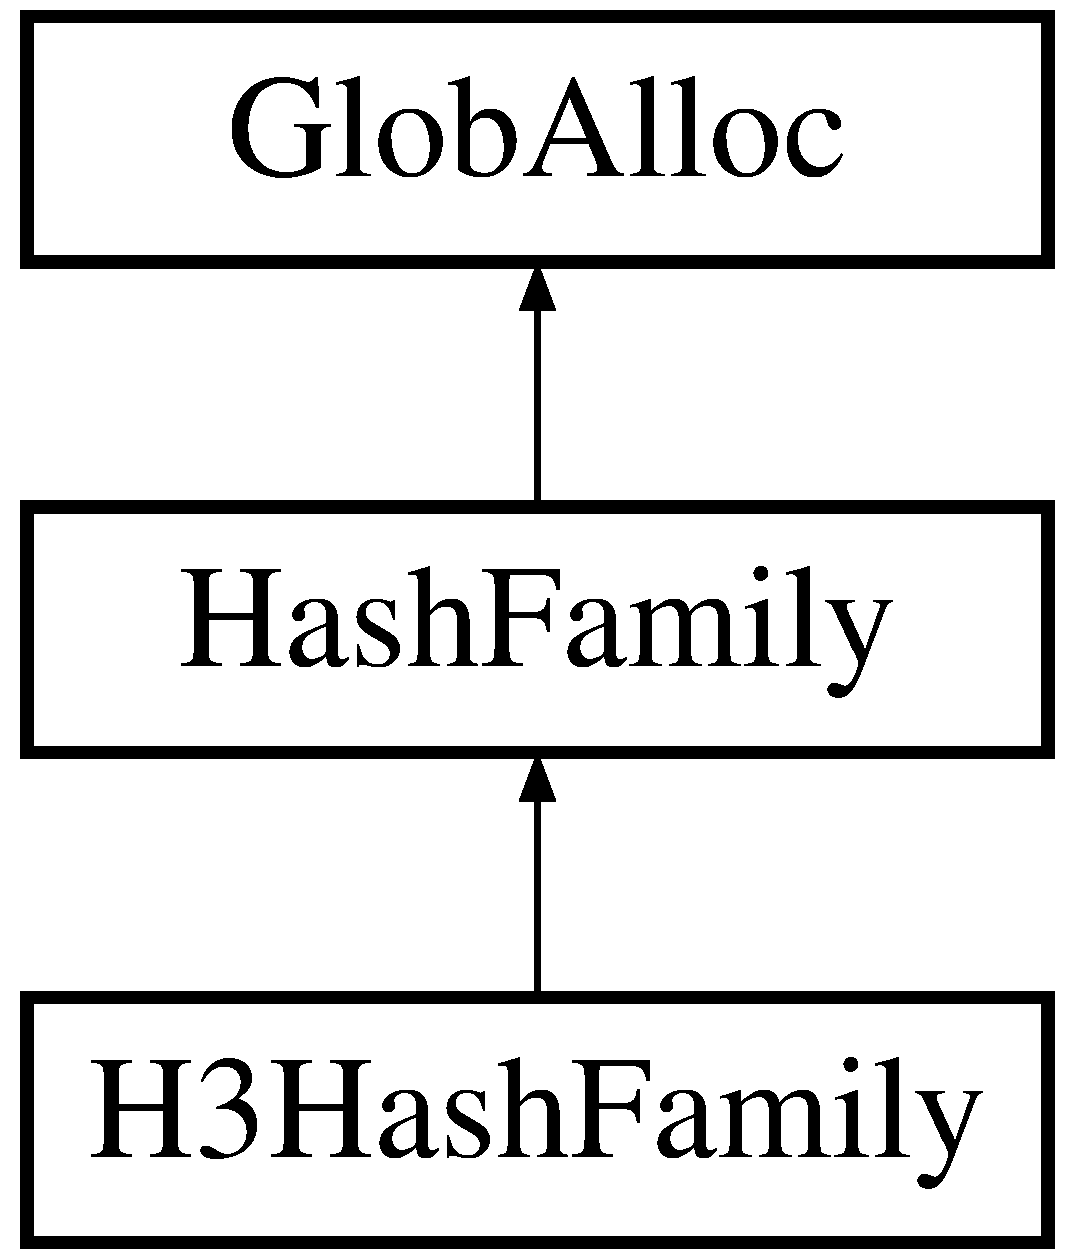
\includegraphics[height=3.000000cm]{classH3HashFamily}
\end{center}
\end{figure}
\subsection*{Public Member Functions}
\begin{DoxyCompactItemize}
\item 
\hyperlink{classH3HashFamily_a1702cad8d3646b91351f3e3ca34a73e9}{H3\-Hash\-Family} (uint32\-\_\-t num\-Functions, uint32\-\_\-t output\-Bits, uint64\-\_\-t rand\-Seed=123132127)
\item 
\hypertarget{classH3HashFamily_afc78fb6206e1065e3219db45249a625c}{uint64\-\_\-t {\bfseries hash} (uint32\-\_\-t id, uint64\-\_\-t val)}\label{classH3HashFamily_afc78fb6206e1065e3219db45249a625c}

\end{DoxyCompactItemize}


\subsection{Constructor \& Destructor Documentation}
\hypertarget{classH3HashFamily_a1702cad8d3646b91351f3e3ca34a73e9}{\index{H3\-Hash\-Family@{H3\-Hash\-Family}!H3\-Hash\-Family@{H3\-Hash\-Family}}
\index{H3\-Hash\-Family@{H3\-Hash\-Family}!H3HashFamily@{H3\-Hash\-Family}}
\subsubsection[{H3\-Hash\-Family}]{\setlength{\rightskip}{0pt plus 5cm}H3\-Hash\-Family\-::\-H3\-Hash\-Family (
\begin{DoxyParamCaption}
\item[{uint32\-\_\-t}]{num\-Functions, }
\item[{uint32\-\_\-t}]{output\-Bits, }
\item[{uint64\-\_\-t}]{rand\-Seed = {\ttfamily 123132127}}
\end{DoxyParamCaption}
)}}\label{classH3HashFamily_a1702cad8d3646b91351f3e3ca34a73e9}
\$lic\$ Copyright (C) 2012-\/2015 by Massachusetts Institute of Technology Copyright (C) 2010-\/2013 by The Board of Trustees of Stanford University

This file is part of zsim.

zsim is free software; you can redistribute it and/or modify it under the terms of the G\-N\-U General Public License as published by the Free Software Foundation, version 2.

If you use this software in your research, we request that you reference the zsim paper (\char`\"{}\-Z\-Sim\-: Fast and Accurate Microarchitectural Simulation of
\-Thousand-\/\-Core Systems\char`\"{}, Sanchez and Kozyrakis, I\-S\-C\-A-\/40, June 2013) as the source of the simulator in any publications that use this software, and that you send us a citation of your work.

zsim is distributed in the hope that it will be useful, but W\-I\-T\-H\-O\-U\-T A\-N\-Y W\-A\-R\-R\-A\-N\-T\-Y; without even the implied warranty of M\-E\-R\-C\-H\-A\-N\-T\-A\-B\-I\-L\-I\-T\-Y or F\-I\-T\-N\-E\-S\-S F\-O\-R A P\-A\-R\-T\-I\-C\-U\-L\-A\-R P\-U\-R\-P\-O\-S\-E. See the G\-N\-U General Public License for more details.

You should have received a copy of the G\-N\-U General Public License along with this program. If not, see \href{http://www.gnu.org/licenses/}{\tt http\-://www.\-gnu.\-org/licenses/}. 

The documentation for this class was generated from the following files\-:\begin{DoxyCompactItemize}
\item 
hash.\-h\item 
hash.\-cpp\end{DoxyCompactItemize}

\hypertarget{classHashFamily}{\section{Hash\-Family Class Reference}
\label{classHashFamily}\index{Hash\-Family@{Hash\-Family}}
}


{\ttfamily \#include $<$hash.\-h$>$}

Inheritance diagram for Hash\-Family\-:\begin{figure}[H]
\begin{center}
\leavevmode
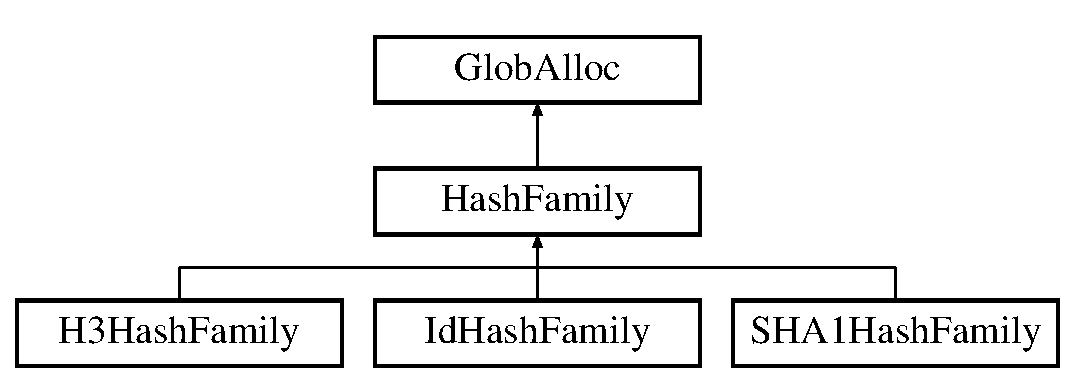
\includegraphics[height=3.000000cm]{classHashFamily}
\end{center}
\end{figure}
\subsection*{Public Member Functions}
\begin{DoxyCompactItemize}
\item 
\hypertarget{classHashFamily_adccfa4b4e61886a5b6ffc6e7797367e1}{virtual uint64\-\_\-t {\bfseries hash} (uint32\-\_\-t id, uint64\-\_\-t val)=0}\label{classHashFamily_adccfa4b4e61886a5b6ffc6e7797367e1}

\end{DoxyCompactItemize}


\subsection{Detailed Description}
\$lic\$ Copyright (C) 2012-\/2015 by Massachusetts Institute of Technology Copyright (C) 2010-\/2013 by The Board of Trustees of Stanford University

This file is part of zsim.

zsim is free software; you can redistribute it and/or modify it under the terms of the G\-N\-U General Public License as published by the Free Software Foundation, version 2.

If you use this software in your research, we request that you reference the zsim paper (\char`\"{}\-Z\-Sim\-: Fast and Accurate Microarchitectural Simulation of
\-Thousand-\/\-Core Systems\char`\"{}, Sanchez and Kozyrakis, I\-S\-C\-A-\/40, June 2013) as the source of the simulator in any publications that use this software, and that you send us a citation of your work.

zsim is distributed in the hope that it will be useful, but W\-I\-T\-H\-O\-U\-T A\-N\-Y W\-A\-R\-R\-A\-N\-T\-Y; without even the implied warranty of M\-E\-R\-C\-H\-A\-N\-T\-A\-B\-I\-L\-I\-T\-Y or F\-I\-T\-N\-E\-S\-S F\-O\-R A P\-A\-R\-T\-I\-C\-U\-L\-A\-R P\-U\-R\-P\-O\-S\-E. See the G\-N\-U General Public License for more details.

You should have received a copy of the G\-N\-U General Public License along with this program. If not, see \href{http://www.gnu.org/licenses/}{\tt http\-://www.\-gnu.\-org/licenses/}. 

The documentation for this class was generated from the following file\-:\begin{DoxyCompactItemize}
\item 
hash.\-h\end{DoxyCompactItemize}

\hypertarget{classHDF5Backend}{\section{H\-D\-F5\-Backend Class Reference}
\label{classHDF5Backend}\index{H\-D\-F5\-Backend@{H\-D\-F5\-Backend}}
}
Inheritance diagram for H\-D\-F5\-Backend\-:\begin{figure}[H]
\begin{center}
\leavevmode
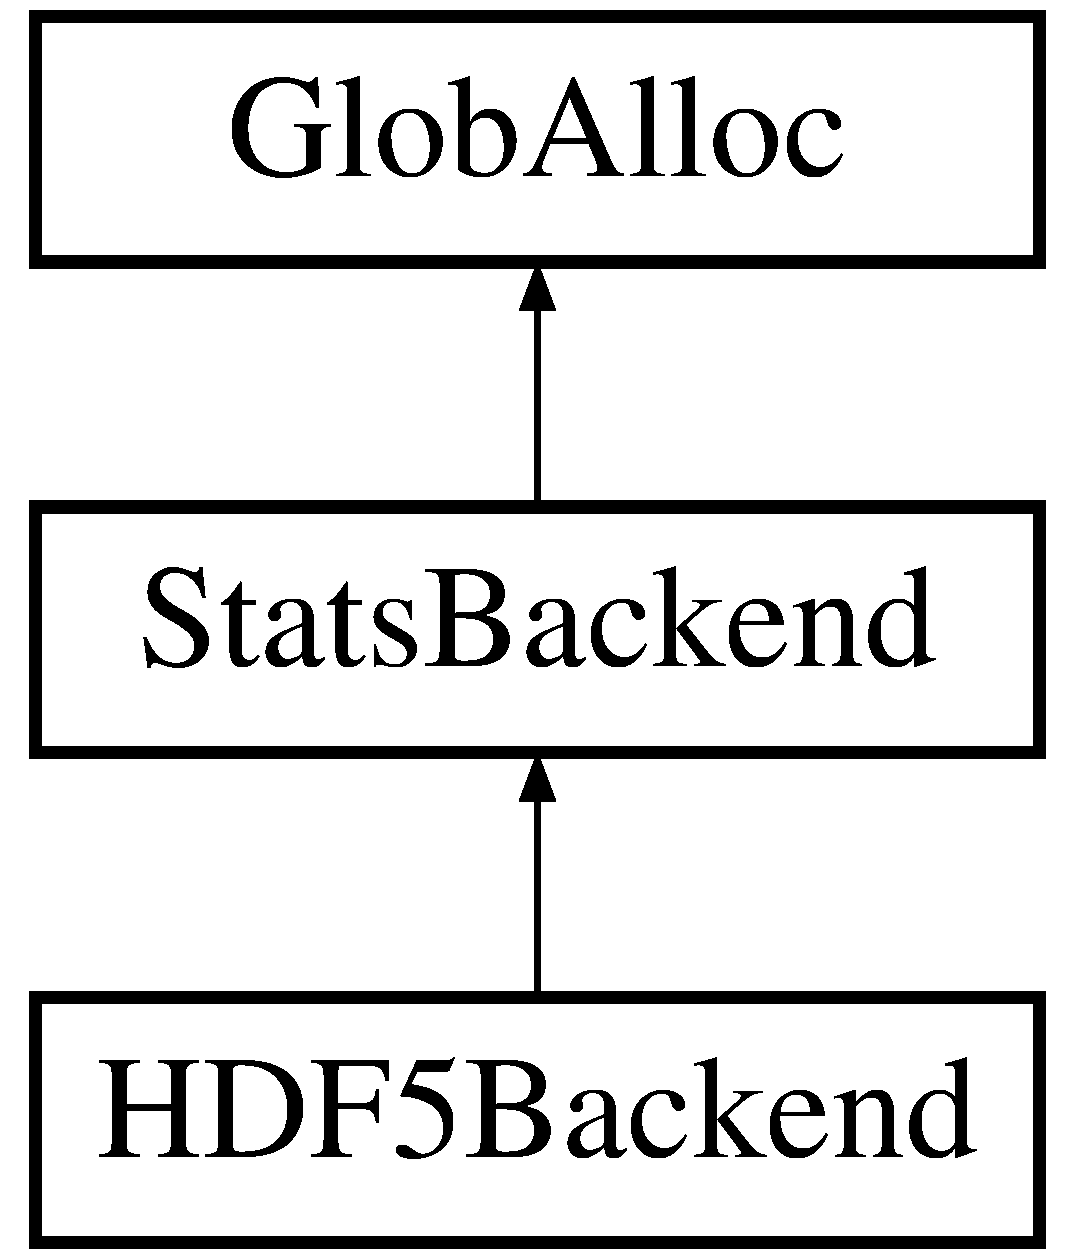
\includegraphics[height=3.000000cm]{classHDF5Backend}
\end{center}
\end{figure}
\subsection*{Public Member Functions}
\begin{DoxyCompactItemize}
\item 
\hypertarget{classHDF5Backend_ac12e84e1c4cc5ce59b9fe94192587fdd}{{\bfseries H\-D\-F5\-Backend} (const char $\ast$filename, \hyperlink{classAggregateStat}{Aggregate\-Stat} $\ast$root\-Stat, size\-\_\-t bytes\-Per\-Write, bool skip\-Vectors, bool sum\-Regular\-Aggregates)}\label{classHDF5Backend_ac12e84e1c4cc5ce59b9fe94192587fdd}

\item 
\hypertarget{classHDF5Backend_aa30ec81d35765cc8abbf2f1653070e25}{virtual void {\bfseries dump} (bool buffered)}\label{classHDF5Backend_aa30ec81d35765cc8abbf2f1653070e25}

\end{DoxyCompactItemize}


The documentation for this class was generated from the following files\-:\begin{DoxyCompactItemize}
\item 
stats.\-h\item 
hdf5\-\_\-stats.\-cpp\end{DoxyCompactItemize}

\hypertarget{classHDF5BackendImpl}{\section{H\-D\-F5\-Backend\-Impl Class Reference}
\label{classHDF5BackendImpl}\index{H\-D\-F5\-Backend\-Impl@{H\-D\-F5\-Backend\-Impl}}
}
Inheritance diagram for H\-D\-F5\-Backend\-Impl\-:\begin{figure}[H]
\begin{center}
\leavevmode
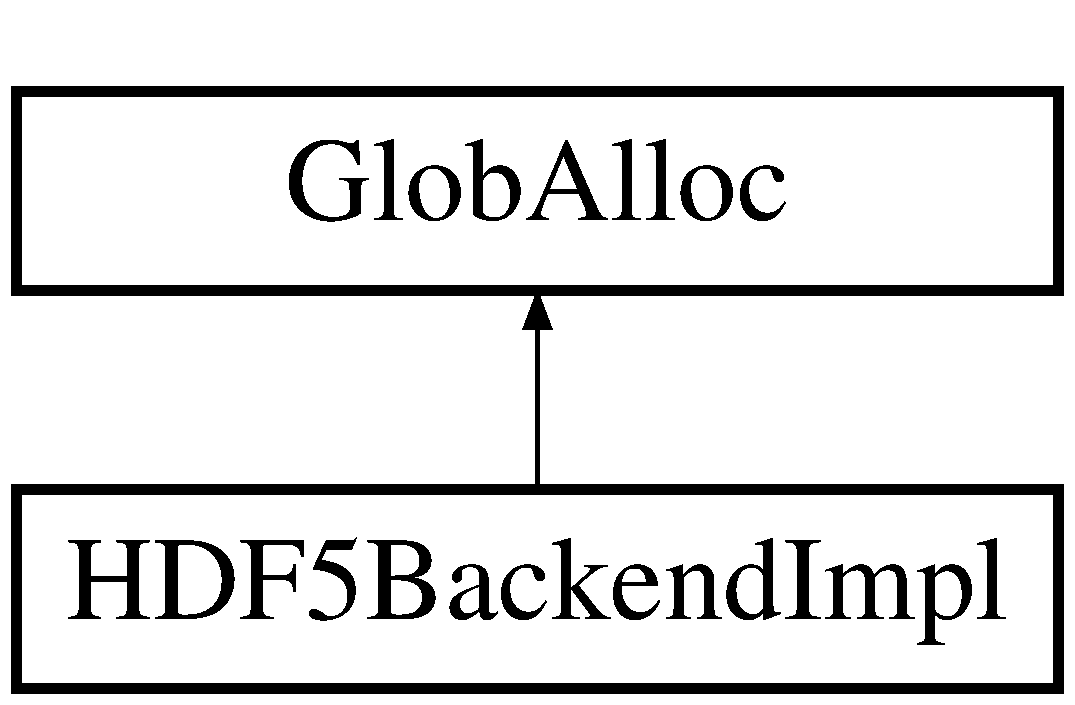
\includegraphics[height=2.000000cm]{classHDF5BackendImpl}
\end{center}
\end{figure}
\subsection*{Public Member Functions}
\begin{DoxyCompactItemize}
\item 
\hypertarget{classHDF5BackendImpl_a43a2ce26bf80e7bf7f8153fb9363c34c}{{\bfseries H\-D\-F5\-Backend\-Impl} (const char $\ast$\-\_\-filename, \hyperlink{classAggregateStat}{Aggregate\-Stat} $\ast$\-\_\-root\-Stat, size\-\_\-t \-\_\-bytes\-Per\-Write, bool \-\_\-skip\-Vectors, bool \-\_\-sum\-Regular\-Aggregates)}\label{classHDF5BackendImpl_a43a2ce26bf80e7bf7f8153fb9363c34c}

\item 
\hypertarget{classHDF5BackendImpl_a8d892e64826c093bcd9e456278f3422e}{void {\bfseries dump} (bool buffered)}\label{classHDF5BackendImpl_a8d892e64826c093bcd9e456278f3422e}

\end{DoxyCompactItemize}


\subsection{Detailed Description}
\$lic\$ Copyright (C) 2012-\/2015 by Massachusetts Institute of Technology Copyright (C) 2010-\/2013 by The Board of Trustees of Stanford University

This file is part of zsim.

zsim is free software; you can redistribute it and/or modify it under the terms of the G\-N\-U General Public License as published by the Free Software Foundation, version 2.

If you use this software in your research, we request that you reference the zsim paper (\char`\"{}\-Z\-Sim\-: Fast and Accurate Microarchitectural Simulation of
\-Thousand-\/\-Core Systems\char`\"{}, Sanchez and Kozyrakis, I\-S\-C\-A-\/40, June 2013) as the source of the simulator in any publications that use this software, and that you send us a citation of your work.

zsim is distributed in the hope that it will be useful, but W\-I\-T\-H\-O\-U\-T A\-N\-Y W\-A\-R\-R\-A\-N\-T\-Y; without even the implied warranty of M\-E\-R\-C\-H\-A\-N\-T\-A\-B\-I\-L\-I\-T\-Y or F\-I\-T\-N\-E\-S\-S F\-O\-R A P\-A\-R\-T\-I\-C\-U\-L\-A\-R P\-U\-R\-P\-O\-S\-E. See the G\-N\-U General Public License for more details.

You should have received a copy of the G\-N\-U General Public License along with this program. If not, see \href{http://www.gnu.org/licenses/}{\tt http\-://www.\-gnu.\-org/licenses/}. Implements the H\-D\-F5 backend. Creates one big table in the file, and writes one row per dump. N\-O\-T\-E\-: Because dump may be called from multiple processes, we close and open the H\-D\-F5 file every dump. This is inefficient, but dumps are not that common anyhow, and we get the ability to read hdf5 files mid-\/simulation. (alternatively, we could have an extra thread exclusively dedicated to writing stats). 

The documentation for this class was generated from the following file\-:\begin{DoxyCompactItemize}
\item 
hdf5\-\_\-stats.\-cpp\end{DoxyCompactItemize}

\hypertarget{classHitEvent}{\section{Hit\-Event Class Reference}
\label{classHitEvent}\index{Hit\-Event@{Hit\-Event}}
}
Inheritance diagram for Hit\-Event\-:\begin{figure}[H]
\begin{center}
\leavevmode
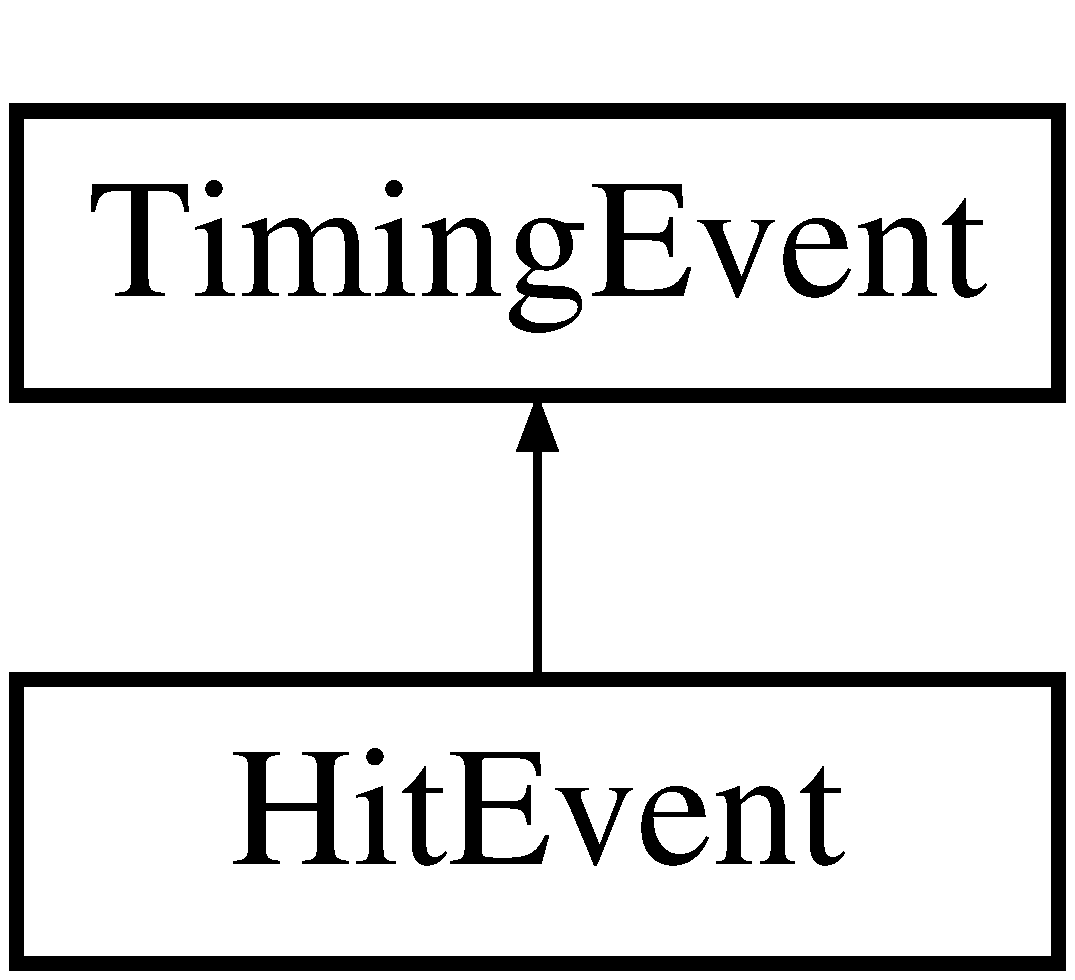
\includegraphics[height=2.000000cm]{classHitEvent}
\end{center}
\end{figure}
\subsection*{Public Member Functions}
\begin{DoxyCompactItemize}
\item 
\hypertarget{classHitEvent_a1a3c3935f5eab43937c515af8d67928d}{{\bfseries Hit\-Event} (\hyperlink{classTimingCache}{Timing\-Cache} $\ast$\-\_\-cache, uint32\-\_\-t post\-Delay, int32\-\_\-t domain)}\label{classHitEvent_a1a3c3935f5eab43937c515af8d67928d}

\item 
\hypertarget{classHitEvent_aa71a04912c1b5df3ae27fb8af88404ae}{void {\bfseries simulate} (uint64\-\_\-t start\-Cycle)}\label{classHitEvent_aa71a04912c1b5df3ae27fb8af88404ae}

\end{DoxyCompactItemize}
\subsection*{Additional Inherited Members}


\subsection{Detailed Description}
\$lic\$ Copyright (C) 2012-\/2015 by Massachusetts Institute of Technology Copyright (C) 2010-\/2013 by The Board of Trustees of Stanford University

This file is part of zsim.

zsim is free software; you can redistribute it and/or modify it under the terms of the G\-N\-U General Public License as published by the Free Software Foundation, version 2.

If you use this software in your research, we request that you reference the zsim paper (\char`\"{}\-Z\-Sim\-: Fast and Accurate Microarchitectural Simulation of
\-Thousand-\/\-Core Systems\char`\"{}, Sanchez and Kozyrakis, I\-S\-C\-A-\/40, June 2013) as the source of the simulator in any publications that use this software, and that you send us a citation of your work.

zsim is distributed in the hope that it will be useful, but W\-I\-T\-H\-O\-U\-T A\-N\-Y W\-A\-R\-R\-A\-N\-T\-Y; without even the implied warranty of M\-E\-R\-C\-H\-A\-N\-T\-A\-B\-I\-L\-I\-T\-Y or F\-I\-T\-N\-E\-S\-S F\-O\-R A P\-A\-R\-T\-I\-C\-U\-L\-A\-R P\-U\-R\-P\-O\-S\-E. See the G\-N\-U General Public License for more details.

You should have received a copy of the G\-N\-U General Public License along with this program. If not, see \href{http://www.gnu.org/licenses/}{\tt http\-://www.\-gnu.\-org/licenses/}. 

The documentation for this class was generated from the following file\-:\begin{DoxyCompactItemize}
\item 
timing\-\_\-cache.\-cpp\end{DoxyCompactItemize}

\hypertarget{structMemParam_1_1IDDs}{\section{Mem\-Param\-:\-:I\-D\-Ds Struct Reference}
\label{structMemParam_1_1IDDs}\index{Mem\-Param\-::\-I\-D\-Ds@{Mem\-Param\-::\-I\-D\-Ds}}
}
\subsection*{Public Attributes}
\begin{DoxyCompactItemize}
\item 
\hypertarget{structMemParam_1_1IDDs_a8fcfe9e934164ff83e346230f169dabf}{uint32\-\_\-t {\bfseries I\-D\-D0}}\label{structMemParam_1_1IDDs_a8fcfe9e934164ff83e346230f169dabf}

\item 
\hypertarget{structMemParam_1_1IDDs_a4b7c8f54fa62e4aff3e19b75bf6de6c4}{uint32\-\_\-t {\bfseries I\-D\-D2\-P}}\label{structMemParam_1_1IDDs_a4b7c8f54fa62e4aff3e19b75bf6de6c4}

\item 
\hypertarget{structMemParam_1_1IDDs_ac9edff647fcc8a29e5dff344f666f882}{uint32\-\_\-t {\bfseries I\-D\-D2\-N}}\label{structMemParam_1_1IDDs_ac9edff647fcc8a29e5dff344f666f882}

\item 
\hypertarget{structMemParam_1_1IDDs_a82d176b52f517b4454717022f2eb90cf}{uint32\-\_\-t {\bfseries I\-D\-D3\-P}}\label{structMemParam_1_1IDDs_a82d176b52f517b4454717022f2eb90cf}

\item 
\hypertarget{structMemParam_1_1IDDs_aa3070fa8a506b2c430330c7cc64d86ae}{uint32\-\_\-t {\bfseries I\-D\-D3\-N}}\label{structMemParam_1_1IDDs_aa3070fa8a506b2c430330c7cc64d86ae}

\item 
\hypertarget{structMemParam_1_1IDDs_a3f407bf4130cb9cd19debd2c211c6c2c}{uint32\-\_\-t {\bfseries I\-D\-D4\-R}}\label{structMemParam_1_1IDDs_a3f407bf4130cb9cd19debd2c211c6c2c}

\item 
\hypertarget{structMemParam_1_1IDDs_af5352db154c1e132d9f2f9d9f667d2a6}{uint32\-\_\-t {\bfseries I\-D\-D4\-W}}\label{structMemParam_1_1IDDs_af5352db154c1e132d9f2f9d9f667d2a6}

\item 
\hypertarget{structMemParam_1_1IDDs_afcbefd971416f3bf373fe52f392f8eee}{uint32\-\_\-t {\bfseries I\-D\-D5}}\label{structMemParam_1_1IDDs_afcbefd971416f3bf373fe52f392f8eee}

\end{DoxyCompactItemize}


The documentation for this struct was generated from the following file\-:\begin{DoxyCompactItemize}
\item 
detailed\-\_\-mem\-\_\-params.\-h\end{DoxyCompactItemize}

\hypertarget{classIdealLRUArray}{\section{Ideal\-L\-R\-U\-Array Class Reference}
\label{classIdealLRUArray}\index{Ideal\-L\-R\-U\-Array@{Ideal\-L\-R\-U\-Array}}
}


{\ttfamily \#include $<$ideal\-\_\-arrays.\-h$>$}

Inheritance diagram for Ideal\-L\-R\-U\-Array\-:\begin{figure}[H]
\begin{center}
\leavevmode
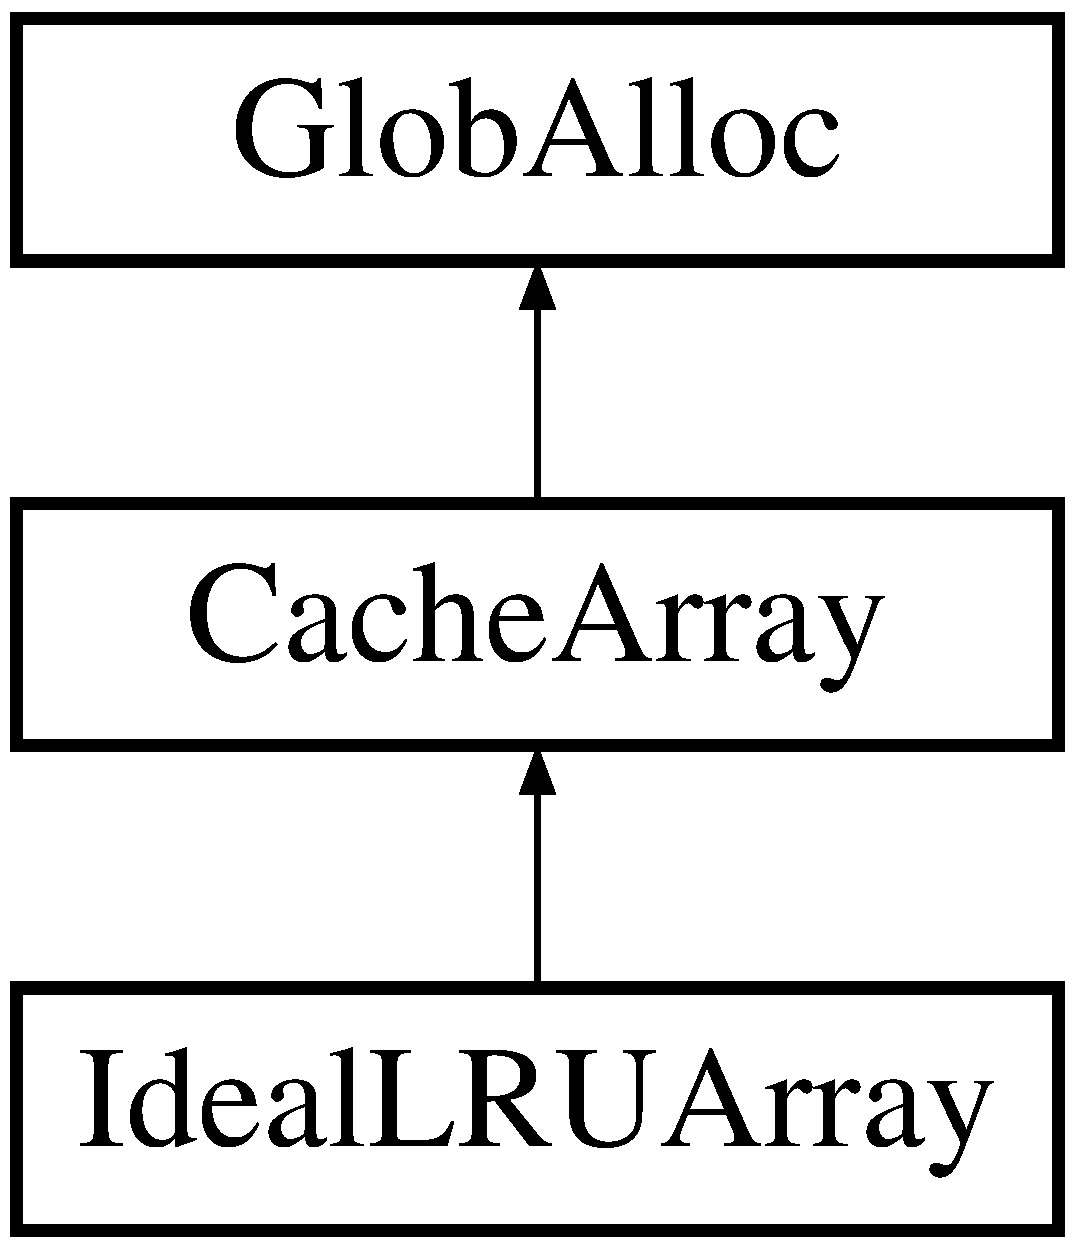
\includegraphics[height=3.000000cm]{classIdealLRUArray}
\end{center}
\end{figure}
\subsection*{Public Member Functions}
\begin{DoxyCompactItemize}
\item 
\hypertarget{classIdealLRUArray_af1a4102b2fef0241d63f0e801e89f2e1}{{\bfseries Ideal\-L\-R\-U\-Array} (uint32\-\_\-t \-\_\-num\-Lines)}\label{classIdealLRUArray_af1a4102b2fef0241d63f0e801e89f2e1}

\item 
\hypertarget{classIdealLRUArray_aee6f323e0bc32079036d7e4a9c6933a1}{int32\-\_\-t {\bfseries lookup} (const Address line\-Addr, const \hyperlink{structMemReq}{Mem\-Req} $\ast$req, bool update\-Replacement)}\label{classIdealLRUArray_aee6f323e0bc32079036d7e4a9c6933a1}

\item 
\hypertarget{classIdealLRUArray_a1bbd715a516bd619a7616278af19c835}{uint32\-\_\-t {\bfseries preinsert} (const Address line\-Addr, const \hyperlink{structMemReq}{Mem\-Req} $\ast$req, Address $\ast$wb\-Line\-Addr)}\label{classIdealLRUArray_a1bbd715a516bd619a7616278af19c835}

\item 
\hypertarget{classIdealLRUArray_a7bb8b248770283b7083a242d825ff795}{void {\bfseries postinsert} (const Address line\-Addr, const \hyperlink{structMemReq}{Mem\-Req} $\ast$req, uint32\-\_\-t line\-Id)}\label{classIdealLRUArray_a7bb8b248770283b7083a242d825ff795}

\item 
\hypertarget{classIdealLRUArray_ab4ed72c6342be5ff2e6c47bab63068ce}{\hyperlink{classReplPolicy}{Repl\-Policy} $\ast$ {\bfseries get\-R\-P} () const }\label{classIdealLRUArray_ab4ed72c6342be5ff2e6c47bab63068ce}

\item 
\hypertarget{classIdealLRUArray_a7dfad52e5897a8816334c038d103fd3a}{void {\bfseries set\-C\-C} (\hyperlink{classCC}{C\-C} $\ast$\-\_\-cc)}\label{classIdealLRUArray_a7dfad52e5897a8816334c038d103fd3a}

\end{DoxyCompactItemize}


\subsection{Detailed Description}
\$lic\$ Copyright (C) 2012-\/2015 by Massachusetts Institute of Technology Copyright (C) 2010-\/2013 by The Board of Trustees of Stanford University

This file is part of zsim.

zsim is free software; you can redistribute it and/or modify it under the terms of the G\-N\-U General Public License as published by the Free Software Foundation, version 2.

If you use this software in your research, we request that you reference the zsim paper (\char`\"{}\-Z\-Sim\-: Fast and Accurate Microarchitectural Simulation of
\-Thousand-\/\-Core Systems\char`\"{}, Sanchez and Kozyrakis, I\-S\-C\-A-\/40, June 2013) as the source of the simulator in any publications that use this software, and that you send us a citation of your work.

zsim is distributed in the hope that it will be useful, but W\-I\-T\-H\-O\-U\-T A\-N\-Y W\-A\-R\-R\-A\-N\-T\-Y; without even the implied warranty of M\-E\-R\-C\-H\-A\-N\-T\-A\-B\-I\-L\-I\-T\-Y or F\-I\-T\-N\-E\-S\-S F\-O\-R A P\-A\-R\-T\-I\-C\-U\-L\-A\-R P\-U\-R\-P\-O\-S\-E. See the G\-N\-U General Public License for more details.

You should have received a copy of the G\-N\-U General Public License along with this program. If not, see \href{http://www.gnu.org/licenses/}{\tt http\-://www.\-gnu.\-org/licenses/}. 

The documentation for this class was generated from the following file\-:\begin{DoxyCompactItemize}
\item 
ideal\-\_\-arrays.\-h\end{DoxyCompactItemize}

\hypertarget{classIdealLRUPartArray}{\section{Ideal\-L\-R\-U\-Part\-Array Class Reference}
\label{classIdealLRUPartArray}\index{Ideal\-L\-R\-U\-Part\-Array@{Ideal\-L\-R\-U\-Part\-Array}}
}
Inheritance diagram for Ideal\-L\-R\-U\-Part\-Array\-:\begin{figure}[H]
\begin{center}
\leavevmode
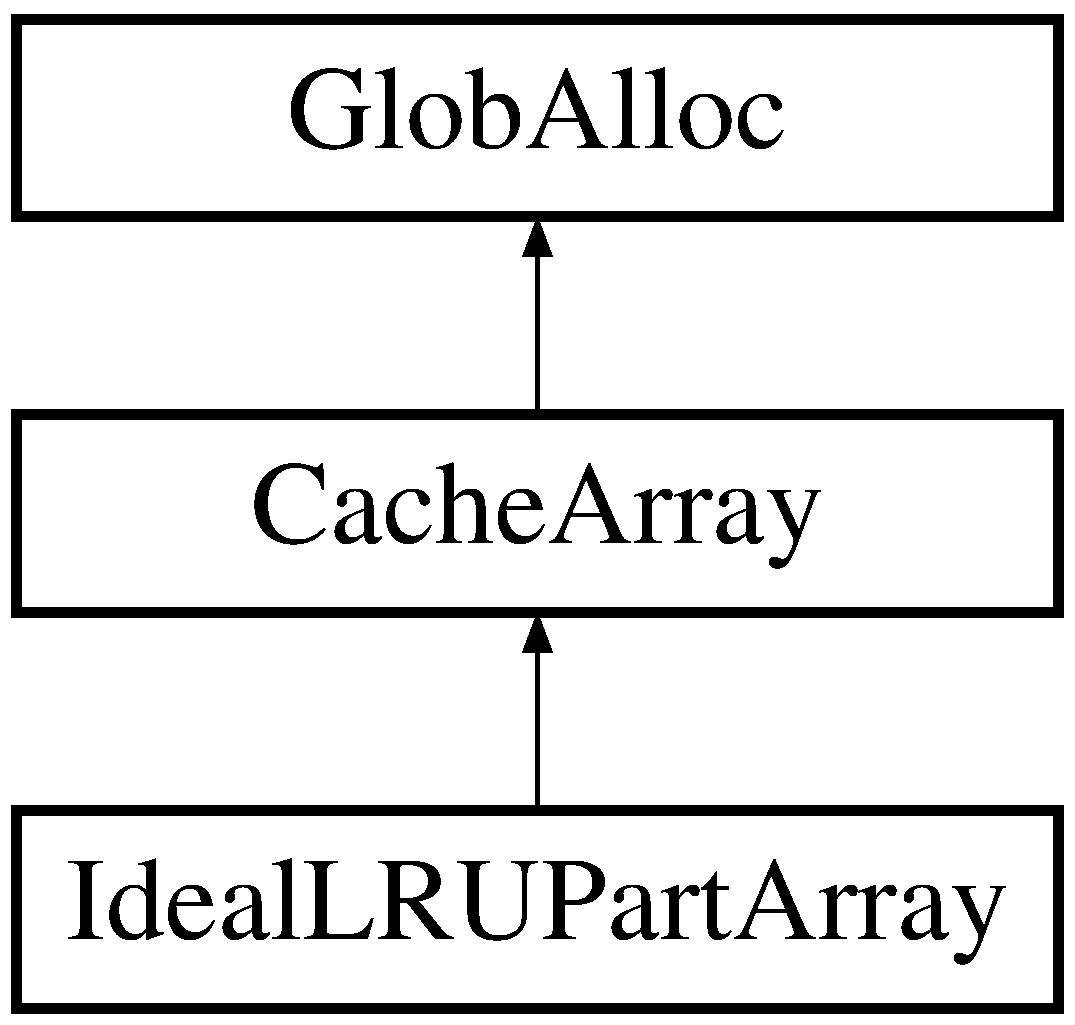
\includegraphics[height=3.000000cm]{classIdealLRUPartArray}
\end{center}
\end{figure}
\subsection*{Public Member Functions}
\begin{DoxyCompactItemize}
\item 
\hypertarget{classIdealLRUPartArray_a568cfad2ecdcbb3252d9aea18ebe89d5}{{\bfseries Ideal\-L\-R\-U\-Part\-Array} (uint32\-\_\-t \-\_\-num\-Lines, \hyperlink{classIdealLRUPartReplPolicy}{Ideal\-L\-R\-U\-Part\-Repl\-Policy} $\ast$\-\_\-rp)}\label{classIdealLRUPartArray_a568cfad2ecdcbb3252d9aea18ebe89d5}

\item 
\hypertarget{classIdealLRUPartArray_aa73a82fc679c92237e03bb21ec260ee9}{int32\-\_\-t {\bfseries lookup} (const Address line\-Addr, const \hyperlink{structMemReq}{Mem\-Req} $\ast$req, bool update\-Replacement)}\label{classIdealLRUPartArray_aa73a82fc679c92237e03bb21ec260ee9}

\item 
\hypertarget{classIdealLRUPartArray_a2b01290a2a0f8748057e1fa2a52cbea9}{uint32\-\_\-t {\bfseries preinsert} (const Address line\-Addr, const \hyperlink{structMemReq}{Mem\-Req} $\ast$req, Address $\ast$wb\-Line\-Addr)}\label{classIdealLRUPartArray_a2b01290a2a0f8748057e1fa2a52cbea9}

\item 
\hypertarget{classIdealLRUPartArray_ae3bd83a71bc6234f2c954b54b73c5171}{void {\bfseries postinsert} (const Address line\-Addr, const \hyperlink{structMemReq}{Mem\-Req} $\ast$req, uint32\-\_\-t line\-Id)}\label{classIdealLRUPartArray_ae3bd83a71bc6234f2c954b54b73c5171}

\end{DoxyCompactItemize}


The documentation for this class was generated from the following file\-:\begin{DoxyCompactItemize}
\item 
ideal\-\_\-arrays.\-h\end{DoxyCompactItemize}

\hypertarget{classIdealLRUPartReplPolicy}{\section{Ideal\-L\-R\-U\-Part\-Repl\-Policy Class Reference}
\label{classIdealLRUPartReplPolicy}\index{Ideal\-L\-R\-U\-Part\-Repl\-Policy@{Ideal\-L\-R\-U\-Part\-Repl\-Policy}}
}
Inheritance diagram for Ideal\-L\-R\-U\-Part\-Repl\-Policy\-:\begin{figure}[H]
\begin{center}
\leavevmode
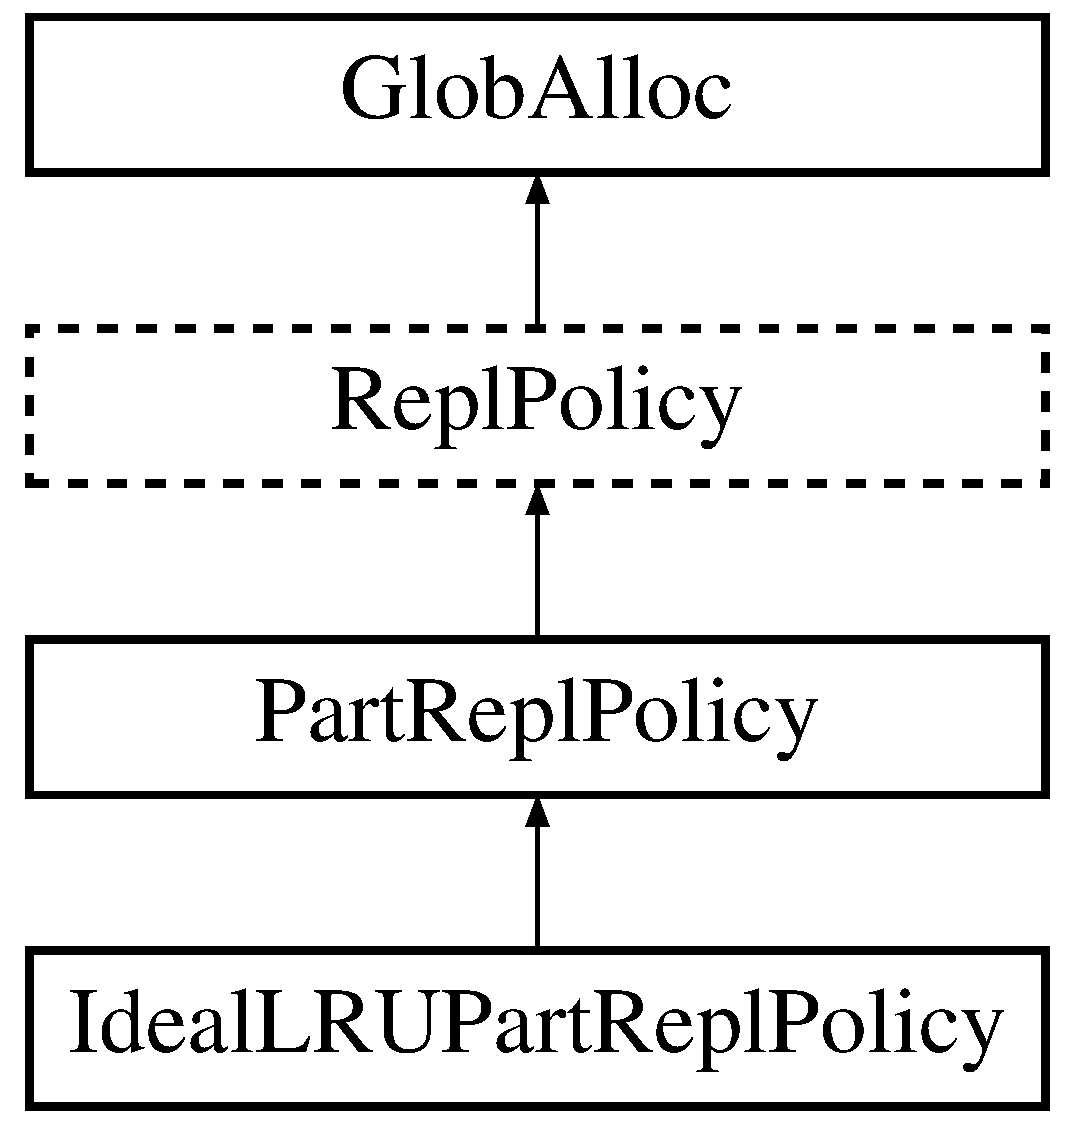
\includegraphics[height=4.000000cm]{classIdealLRUPartReplPolicy}
\end{center}
\end{figure}
\subsection*{Classes}
\begin{DoxyCompactItemize}
\item 
struct \hyperlink{structIdealLRUPartReplPolicy_1_1Entry}{Entry}
\item 
struct \hyperlink{structIdealLRUPartReplPolicy_1_1IdPartInfo}{Id\-Part\-Info}
\end{DoxyCompactItemize}
\subsection*{Public Member Functions}
\begin{DoxyCompactItemize}
\item 
\hypertarget{classIdealLRUPartReplPolicy_a76f9677a013029f467ae6289b9bb51af}{{\bfseries Ideal\-L\-R\-U\-Part\-Repl\-Policy} (\hyperlink{classPartitionMonitor}{Partition\-Monitor} $\ast$\-\_\-monitor, \hyperlink{classPartMapper}{Part\-Mapper} $\ast$\-\_\-mapper, uint32\-\_\-t \-\_\-num\-Lines, uint32\-\_\-t \-\_\-num\-Buckets)}\label{classIdealLRUPartReplPolicy_a76f9677a013029f467ae6289b9bb51af}

\item 
\hypertarget{classIdealLRUPartReplPolicy_a005d5fcb68c06b418eb0ccebcebcd833}{void {\bfseries init\-Stats} (\hyperlink{classAggregateStat}{Aggregate\-Stat} $\ast$parent\-Stat)}\label{classIdealLRUPartReplPolicy_a005d5fcb68c06b418eb0ccebcebcd833}

\item 
\hypertarget{classIdealLRUPartReplPolicy_acf0338dd7fa8e41ba79f1941aa60a67c}{void {\bfseries set\-Partition\-Sizes} (const uint32\-\_\-t $\ast$sizes)}\label{classIdealLRUPartReplPolicy_acf0338dd7fa8e41ba79f1941aa60a67c}

\item 
\hypertarget{classIdealLRUPartReplPolicy_a8d1da4cc3170f608737c400221114ac5}{void {\bfseries update} (uint32\-\_\-t id, const \hyperlink{structMemReq}{Mem\-Req} $\ast$req)}\label{classIdealLRUPartReplPolicy_a8d1da4cc3170f608737c400221114ac5}

\item 
\hypertarget{classIdealLRUPartReplPolicy_a9c5af0e93e754830f267fa9a5e81967c}{void {\bfseries replaced} (uint32\-\_\-t id)}\label{classIdealLRUPartReplPolicy_a9c5af0e93e754830f267fa9a5e81967c}

\item 
\hypertarget{classIdealLRUPartReplPolicy_a1b346d9edf01a4b38720782ef261ebba}{uint32\-\_\-t {\bfseries rank} (const \hyperlink{structMemReq}{Mem\-Req} $\ast$req)}\label{classIdealLRUPartReplPolicy_a1b346d9edf01a4b38720782ef261ebba}

\item 
\hypertarget{classIdealLRUPartReplPolicy_ae8d8a5ab116569a643ff191bb4848a59}{{\footnotesize template$<$typename C $>$ }\\uint32\-\_\-t {\bfseries rank} (const \hyperlink{structMemReq}{Mem\-Req} $\ast$req, C cands)}\label{classIdealLRUPartReplPolicy_ae8d8a5ab116569a643ff191bb4848a59}

\end{DoxyCompactItemize}
\subsection*{Public Attributes}
\begin{DoxyCompactItemize}
\item 
\hypertarget{classIdealLRUPartReplPolicy_a2f7060fb9a38de21c7312d17bcd0eb0d}{{\bfseries D\-E\-C\-L\-\_\-\-R\-A\-N\-K\-\_\-\-B\-I\-N\-D\-I\-N\-G\-S}}\label{classIdealLRUPartReplPolicy_a2f7060fb9a38de21c7312d17bcd0eb0d}

\end{DoxyCompactItemize}
\subsection*{Protected Attributes}
\begin{DoxyCompactItemize}
\item 
\hypertarget{classIdealLRUPartReplPolicy_a029b993b311cd5d260fc831216105dd5}{\hyperlink{structIdealLRUPartReplPolicy_1_1Entry}{Entry} $\ast$ {\bfseries array}}\label{classIdealLRUPartReplPolicy_a029b993b311cd5d260fc831216105dd5}

\item 
\hypertarget{classIdealLRUPartReplPolicy_a496bfae1cdf483997395949426ca0799}{\hyperlink{structIdealLRUPartReplPolicy_1_1IdPartInfo}{Id\-Part\-Info} $\ast$ {\bfseries part\-Info}}\label{classIdealLRUPartReplPolicy_a496bfae1cdf483997395949426ca0799}

\item 
\hypertarget{classIdealLRUPartReplPolicy_a9dfaf286a21c022139a36ed10d94e3bf}{uint32\-\_\-t {\bfseries partitions}}\label{classIdealLRUPartReplPolicy_a9dfaf286a21c022139a36ed10d94e3bf}

\item 
\hypertarget{classIdealLRUPartReplPolicy_aacf66826621b4e88242f767bafc98705}{uint32\-\_\-t {\bfseries num\-Lines}}\label{classIdealLRUPartReplPolicy_aacf66826621b4e88242f767bafc98705}

\item 
\hypertarget{classIdealLRUPartReplPolicy_aaca59e41a732517b26e87259f0fa589b}{uint32\-\_\-t {\bfseries num\-Buckets}}\label{classIdealLRUPartReplPolicy_aaca59e41a732517b26e87259f0fa589b}

\end{DoxyCompactItemize}


The documentation for this class was generated from the following file\-:\begin{DoxyCompactItemize}
\item 
ideal\-\_\-arrays.\-h\end{DoxyCompactItemize}

\hypertarget{classIdHashFamily}{\section{Id\-Hash\-Family Class Reference}
\label{classIdHashFamily}\index{Id\-Hash\-Family@{Id\-Hash\-Family}}
}
Inheritance diagram for Id\-Hash\-Family\-:\begin{figure}[H]
\begin{center}
\leavevmode
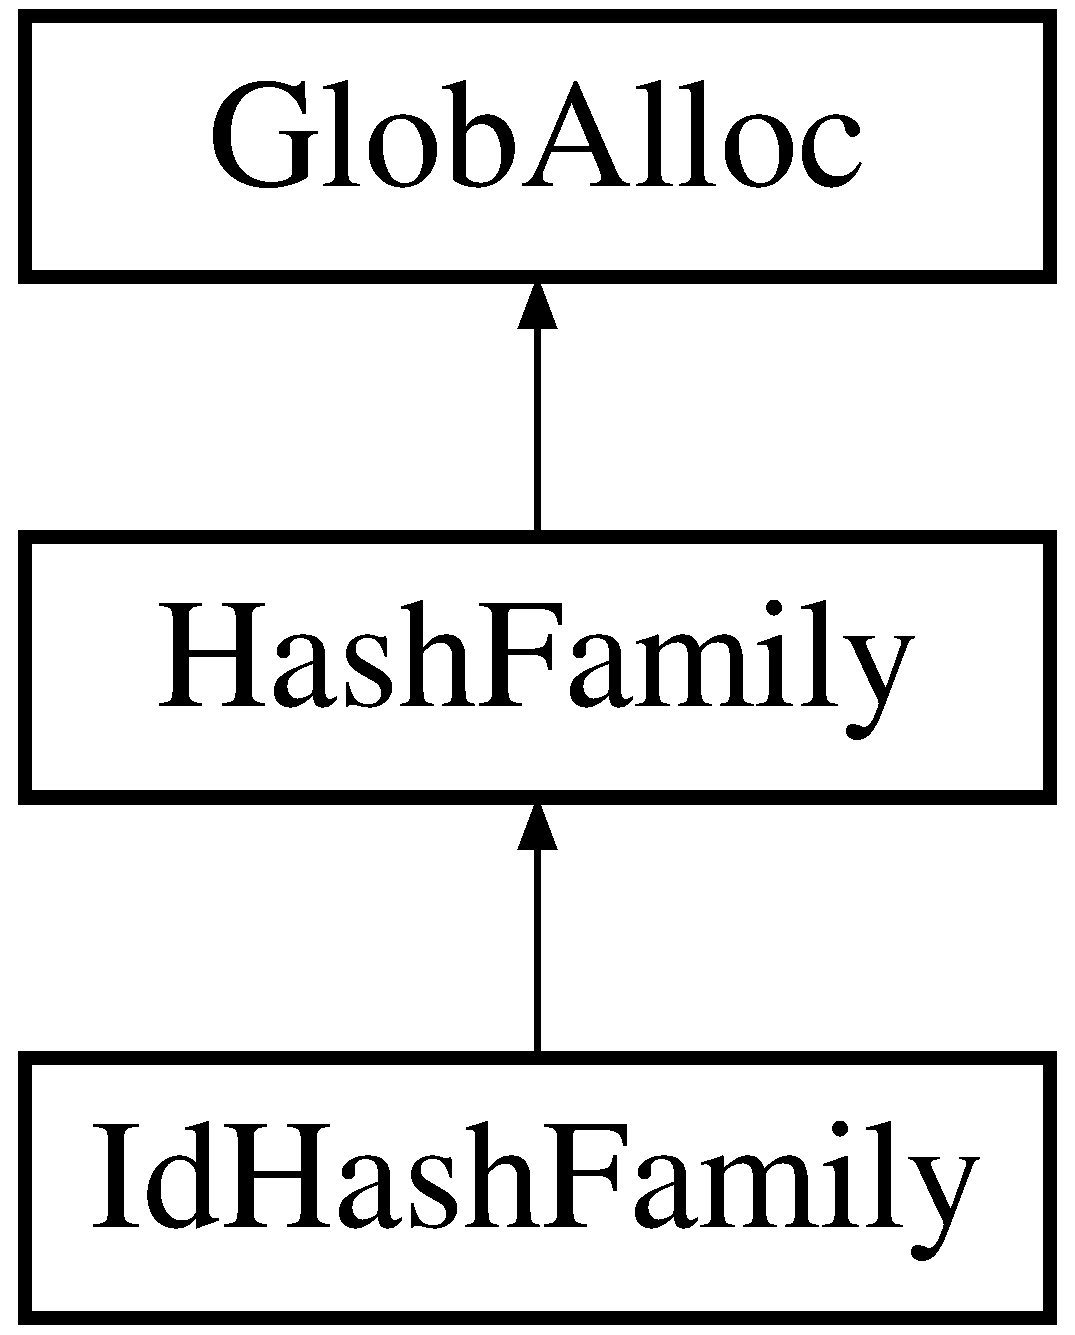
\includegraphics[height=3.000000cm]{classIdHashFamily}
\end{center}
\end{figure}
\subsection*{Public Member Functions}
\begin{DoxyCompactItemize}
\item 
\hypertarget{classIdHashFamily_ad7d484fe595d5f7e94af443ced0e29ea}{uint64\-\_\-t {\bfseries hash} (uint32\-\_\-t id, uint64\-\_\-t val)}\label{classIdHashFamily_ad7d484fe595d5f7e94af443ced0e29ea}

\end{DoxyCompactItemize}


The documentation for this class was generated from the following file\-:\begin{DoxyCompactItemize}
\item 
hash.\-h\end{DoxyCompactItemize}

\hypertarget{structIdealLRUPartReplPolicy_1_1IdPartInfo}{\section{Ideal\-L\-R\-U\-Part\-Repl\-Policy\-:\-:Id\-Part\-Info Struct Reference}
\label{structIdealLRUPartReplPolicy_1_1IdPartInfo}\index{Ideal\-L\-R\-U\-Part\-Repl\-Policy\-::\-Id\-Part\-Info@{Ideal\-L\-R\-U\-Part\-Repl\-Policy\-::\-Id\-Part\-Info}}
}
Inheritance diagram for Ideal\-L\-R\-U\-Part\-Repl\-Policy\-:\-:Id\-Part\-Info\-:\begin{figure}[H]
\begin{center}
\leavevmode
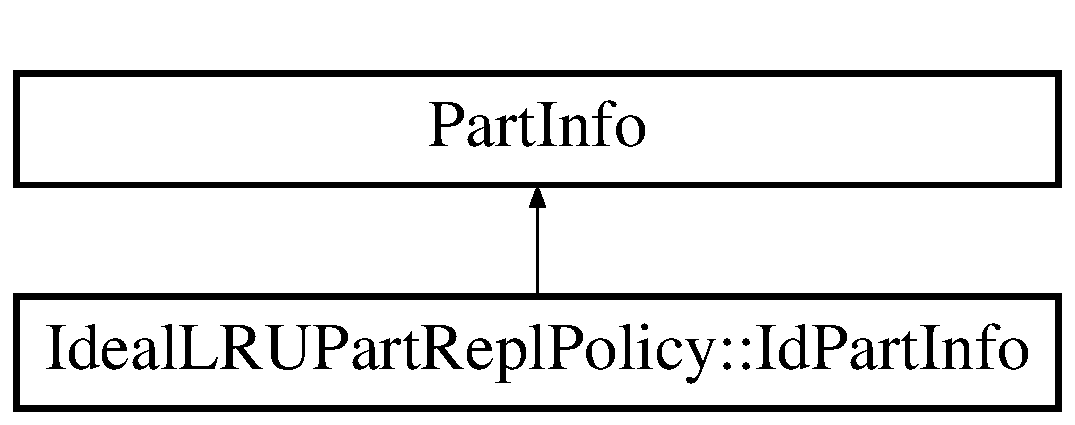
\includegraphics[height=2.000000cm]{structIdealLRUPartReplPolicy_1_1IdPartInfo}
\end{center}
\end{figure}
\subsection*{Public Attributes}
\begin{DoxyCompactItemize}
\item 
\hypertarget{structIdealLRUPartReplPolicy_1_1IdPartInfo_a38eb26210ad5c2699dae9b51fc496516}{\hyperlink{classInList}{In\-List}$<$ \hyperlink{structIdealLRUPartReplPolicy_1_1Entry}{Entry} $>$ {\bfseries lru\-List}}\label{structIdealLRUPartReplPolicy_1_1IdPartInfo_a38eb26210ad5c2699dae9b51fc496516}

\end{DoxyCompactItemize}


The documentation for this struct was generated from the following file\-:\begin{DoxyCompactItemize}
\item 
ideal\-\_\-arrays.\-h\end{DoxyCompactItemize}

\hypertarget{classInList}{\section{In\-List$<$ T $>$ Class Template Reference}
\label{classInList}\index{In\-List$<$ T $>$@{In\-List$<$ T $>$}}
}


{\ttfamily \#include $<$intrusive\-\_\-list.\-h$>$}

\subsection*{Public Member Functions}
\begin{DoxyCompactItemize}
\item 
\hypertarget{classInList_a7a8424b88bf7ead661583383d3f6d482}{bool {\bfseries empty} () const }\label{classInList_a7a8424b88bf7ead661583383d3f6d482}

\item 
\hypertarget{classInList_a2964593cb6b7b50c5224737cac3e54ec}{T $\ast$ {\bfseries front} () const }\label{classInList_a2964593cb6b7b50c5224737cac3e54ec}

\item 
\hypertarget{classInList_a586c6530f61f9e616fab209f905c7de8}{T $\ast$ {\bfseries back} () const }\label{classInList_a586c6530f61f9e616fab209f905c7de8}

\item 
\hypertarget{classInList_a68363298d236385c7e8e8c61884750c2}{void {\bfseries push\-\_\-front} (T $\ast$e)}\label{classInList_a68363298d236385c7e8e8c61884750c2}

\item 
\hypertarget{classInList_a0d0666e7a9551ab6fcfa0b9163566ce6}{void {\bfseries push\-\_\-back} (T $\ast$e)}\label{classInList_a0d0666e7a9551ab6fcfa0b9163566ce6}

\item 
\hypertarget{classInList_ae4e75eaab71a02cbb7bebc00c4b2cd33}{void {\bfseries pop\-\_\-front} ()}\label{classInList_ae4e75eaab71a02cbb7bebc00c4b2cd33}

\item 
\hypertarget{classInList_a0cd4e2762a14cdce257d6d517f4fb5a2}{void {\bfseries pop\-\_\-back} ()}\label{classInList_a0cd4e2762a14cdce257d6d517f4fb5a2}

\item 
\hypertarget{classInList_af9772dd74412cf9f96d64bccf3e15ccc}{void {\bfseries remove} (T $\ast$e)}\label{classInList_af9772dd74412cf9f96d64bccf3e15ccc}

\item 
\hypertarget{classInList_af0fb0a1618368e179e9b8d8e5e2951de}{void {\bfseries insert\-After} (T $\ast$prev, T $\ast$e)}\label{classInList_af0fb0a1618368e179e9b8d8e5e2951de}

\item 
\hypertarget{classInList_afba6855e55a2347623a9a9dd82f23ddd}{size\-\_\-t {\bfseries size} () const }\label{classInList_afba6855e55a2347623a9a9dd82f23ddd}

\end{DoxyCompactItemize}


\subsection{Detailed Description}
\subsubsection*{template$<$typename T$>$class In\-List$<$ T $>$}

\$lic\$ Copyright (C) 2012-\/2015 by Massachusetts Institute of Technology Copyright (C) 2010-\/2013 by The Board of Trustees of Stanford University

This file is part of zsim.

zsim is free software; you can redistribute it and/or modify it under the terms of the G\-N\-U General Public License as published by the Free Software Foundation, version 2.

If you use this software in your research, we request that you reference the zsim paper (\char`\"{}\-Z\-Sim\-: Fast and Accurate Microarchitectural Simulation of
\-Thousand-\/\-Core Systems\char`\"{}, Sanchez and Kozyrakis, I\-S\-C\-A-\/40, June 2013) as the source of the simulator in any publications that use this software, and that you send us a citation of your work.

zsim is distributed in the hope that it will be useful, but W\-I\-T\-H\-O\-U\-T A\-N\-Y W\-A\-R\-R\-A\-N\-T\-Y; without even the implied warranty of M\-E\-R\-C\-H\-A\-N\-T\-A\-B\-I\-L\-I\-T\-Y or F\-I\-T\-N\-E\-S\-S F\-O\-R A P\-A\-R\-T\-I\-C\-U\-L\-A\-R P\-U\-R\-P\-O\-S\-E. See the G\-N\-U General Public License for more details.

You should have received a copy of the G\-N\-U General Public License along with this program. If not, see \href{http://www.gnu.org/licenses/}{\tt http\-://www.\-gnu.\-org/licenses/}. 

The documentation for this class was generated from the following file\-:\begin{DoxyCompactItemize}
\item 
intrusive\-\_\-list.\-h\end{DoxyCompactItemize}

\hypertarget{structInListNode}{\section{In\-List\-Node$<$ T $>$ Struct Template Reference}
\label{structInListNode}\index{In\-List\-Node$<$ T $>$@{In\-List\-Node$<$ T $>$}}
}
\subsection*{Public Member Functions}
\begin{DoxyCompactItemize}
\item 
\hypertarget{structInListNode_a12c5300cc44a7d5358566fa7349c68bf}{void {\bfseries unlink} (\hyperlink{classInList}{In\-List}$<$ T $>$ $\ast$lst)}\label{structInListNode_a12c5300cc44a7d5358566fa7349c68bf}

\item 
\hypertarget{structInListNode_a76c4eacdbb651822ff9c9caba0600082}{void {\bfseries link\-Prev} (T $\ast$p, \hyperlink{classInList}{In\-List}$<$ T $>$ $\ast$lst)}\label{structInListNode_a76c4eacdbb651822ff9c9caba0600082}

\end{DoxyCompactItemize}
\subsection*{Public Attributes}
\begin{DoxyCompactItemize}
\item 
\hypertarget{structInListNode_a285cb71fd2e8dd4055a1d4a618e38032}{T $\ast$ {\bfseries next}}\label{structInListNode_a285cb71fd2e8dd4055a1d4a618e38032}

\item 
\hypertarget{structInListNode_a7d4032af2712b5d542ffa9d800c98a55}{T $\ast$ {\bfseries prev}}\label{structInListNode_a7d4032af2712b5d542ffa9d800c98a55}

\item 
\hypertarget{structInListNode_aa62a10f3d82fc1cdfc0315cab9d674a9}{\hyperlink{classInList}{In\-List}$<$ T $>$ $\ast$ {\bfseries owner}}\label{structInListNode_aa62a10f3d82fc1cdfc0315cab9d674a9}

\end{DoxyCompactItemize}


The documentation for this struct was generated from the following file\-:\begin{DoxyCompactItemize}
\item 
intrusive\-\_\-list.\-h\end{DoxyCompactItemize}

\hypertarget{classInstrDataCorePartMapper}{\section{Instr\-Data\-Core\-Part\-Mapper Class Reference}
\label{classInstrDataCorePartMapper}\index{Instr\-Data\-Core\-Part\-Mapper@{Instr\-Data\-Core\-Part\-Mapper}}
}
Inheritance diagram for Instr\-Data\-Core\-Part\-Mapper\-:\begin{figure}[H]
\begin{center}
\leavevmode
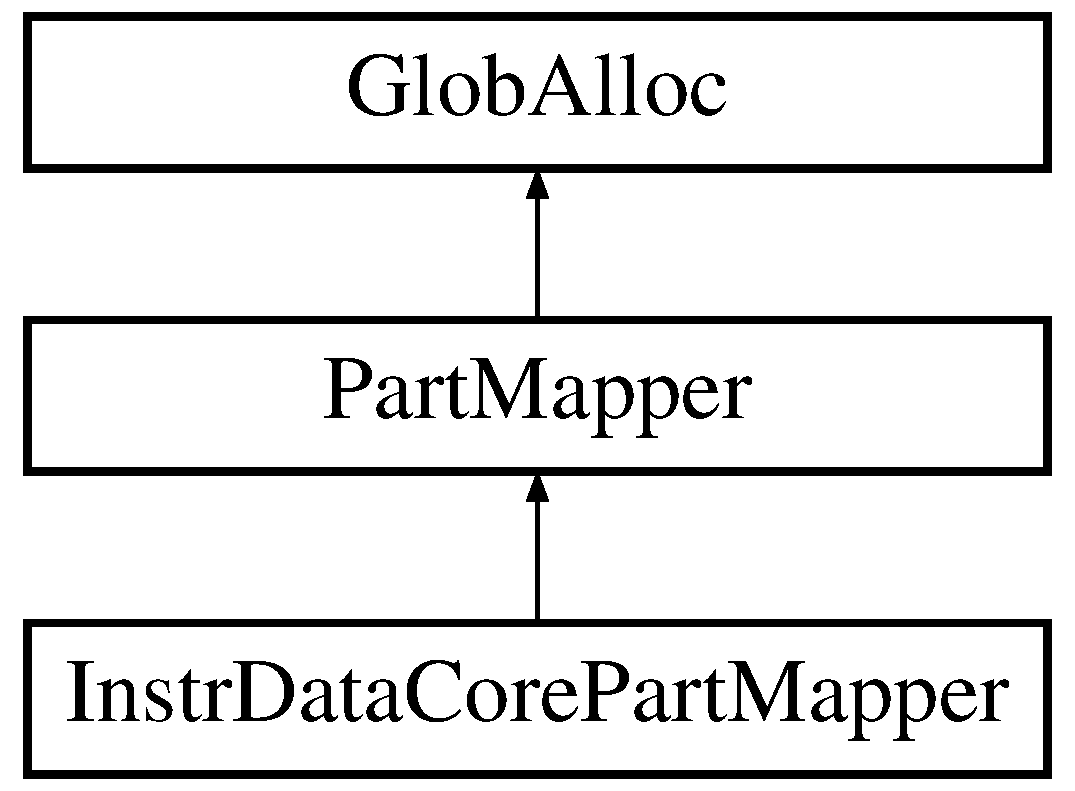
\includegraphics[height=3.000000cm]{classInstrDataCorePartMapper}
\end{center}
\end{figure}
\subsection*{Public Member Functions}
\begin{DoxyCompactItemize}
\item 
\hypertarget{classInstrDataCorePartMapper_a447aa17c7bcfe4ad3955064a51184f11}{{\bfseries Instr\-Data\-Core\-Part\-Mapper} (uint32\-\_\-t \-\_\-num\-Cores)}\label{classInstrDataCorePartMapper_a447aa17c7bcfe4ad3955064a51184f11}

\item 
\hypertarget{classInstrDataCorePartMapper_a1008e1e594fac3edd532babd89b8a4ba}{virtual uint32\-\_\-t {\bfseries get\-Num\-Partitions} ()}\label{classInstrDataCorePartMapper_a1008e1e594fac3edd532babd89b8a4ba}

\item 
\hypertarget{classInstrDataCorePartMapper_ad4610e28ad9d45a77e79bca8d8c434ed}{virtual uint32\-\_\-t {\bfseries get\-Partition} (const \hyperlink{structMemReq}{Mem\-Req} \&req)}\label{classInstrDataCorePartMapper_ad4610e28ad9d45a77e79bca8d8c434ed}

\end{DoxyCompactItemize}


The documentation for this class was generated from the following files\-:\begin{DoxyCompactItemize}
\item 
partition\-\_\-mapper.\-h\item 
partition\-\_\-mapper.\-cpp\end{DoxyCompactItemize}

\hypertarget{classInstrDataPartMapper}{\section{Instr\-Data\-Part\-Mapper Class Reference}
\label{classInstrDataPartMapper}\index{Instr\-Data\-Part\-Mapper@{Instr\-Data\-Part\-Mapper}}
}
Inheritance diagram for Instr\-Data\-Part\-Mapper\-:\begin{figure}[H]
\begin{center}
\leavevmode
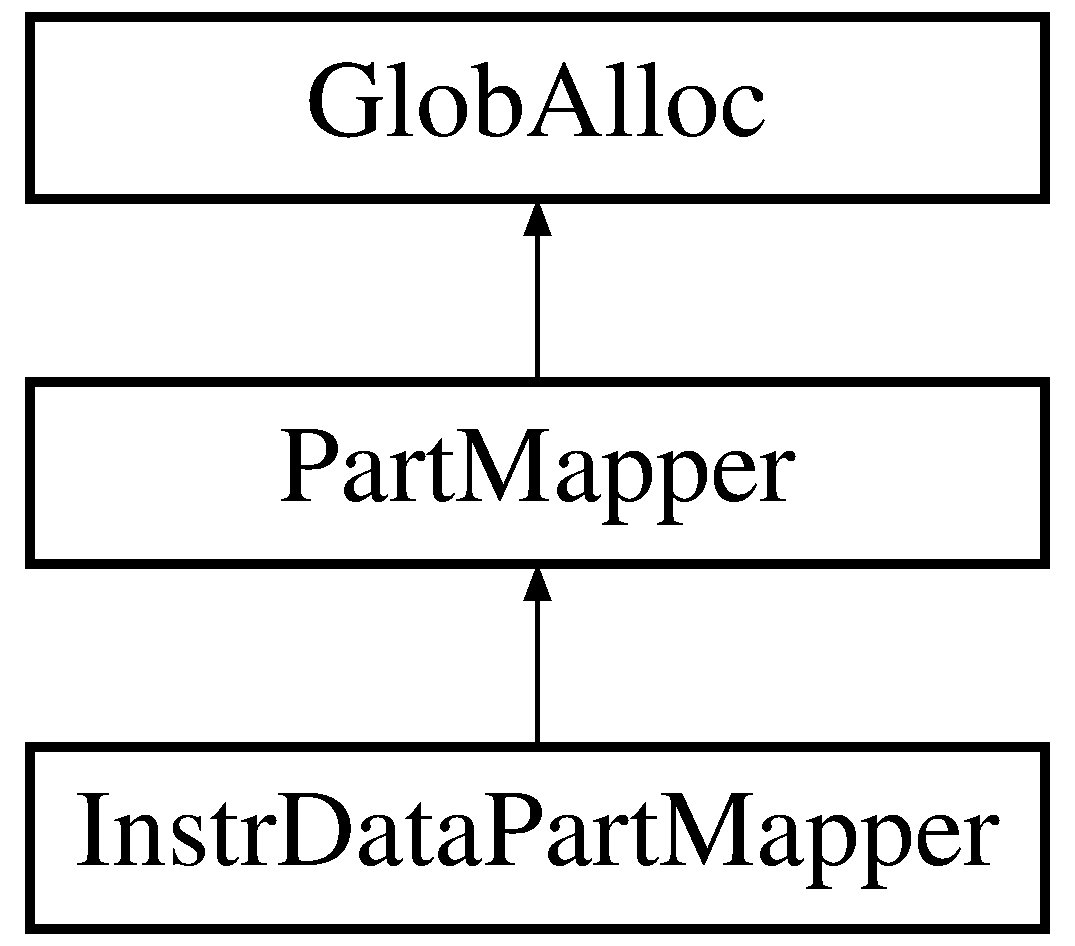
\includegraphics[height=3.000000cm]{classInstrDataPartMapper}
\end{center}
\end{figure}
\subsection*{Public Member Functions}
\begin{DoxyCompactItemize}
\item 
\hypertarget{classInstrDataPartMapper_a64f091e8c3737da1dd7146931f74d926}{virtual uint32\-\_\-t {\bfseries get\-Num\-Partitions} ()}\label{classInstrDataPartMapper_a64f091e8c3737da1dd7146931f74d926}

\item 
\hypertarget{classInstrDataPartMapper_a7edb4dbecd6495a2a29d4896c49958c2}{virtual uint32\-\_\-t {\bfseries get\-Partition} (const \hyperlink{structMemReq}{Mem\-Req} \&req)}\label{classInstrDataPartMapper_a7edb4dbecd6495a2a29d4896c49958c2}

\end{DoxyCompactItemize}


The documentation for this class was generated from the following files\-:\begin{DoxyCompactItemize}
\item 
partition\-\_\-mapper.\-h\item 
partition\-\_\-mapper.\-cpp\end{DoxyCompactItemize}

\hypertarget{classInstrDataProcessPartMapper}{\section{Instr\-Data\-Process\-Part\-Mapper Class Reference}
\label{classInstrDataProcessPartMapper}\index{Instr\-Data\-Process\-Part\-Mapper@{Instr\-Data\-Process\-Part\-Mapper}}
}
Inheritance diagram for Instr\-Data\-Process\-Part\-Mapper\-:\begin{figure}[H]
\begin{center}
\leavevmode
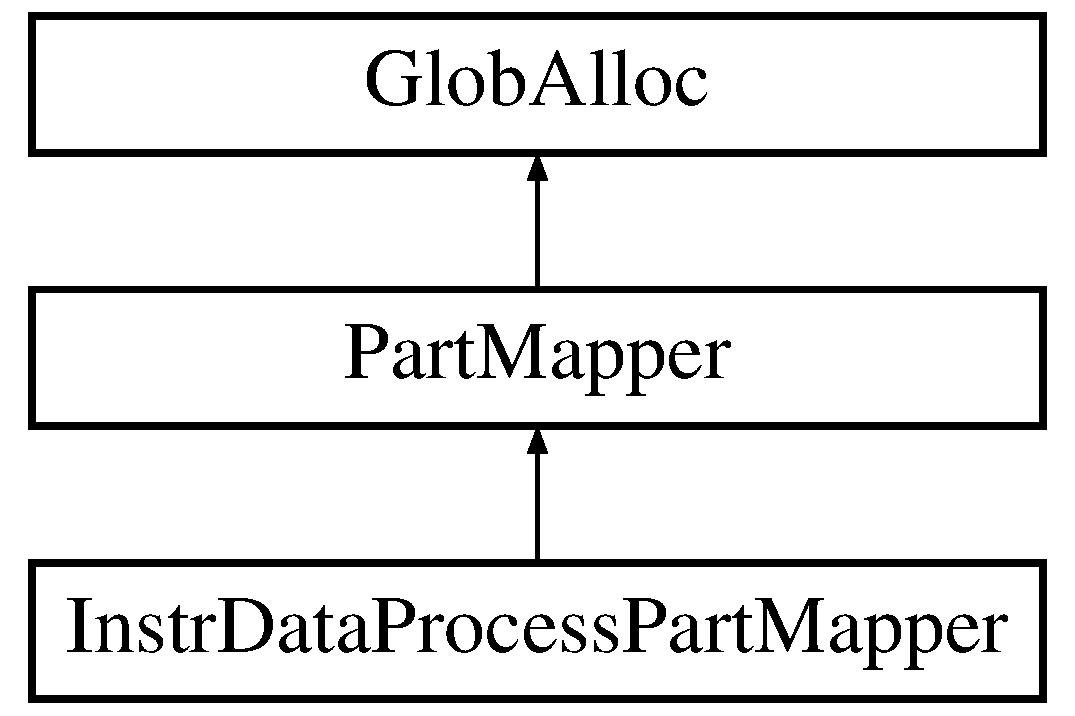
\includegraphics[height=3.000000cm]{classInstrDataProcessPartMapper}
\end{center}
\end{figure}
\subsection*{Public Member Functions}
\begin{DoxyCompactItemize}
\item 
\hypertarget{classInstrDataProcessPartMapper_a9ec951513521573dfa456c182c87d2bd}{{\bfseries Instr\-Data\-Process\-Part\-Mapper} (uint32\-\_\-t \-\_\-num\-Procs)}\label{classInstrDataProcessPartMapper_a9ec951513521573dfa456c182c87d2bd}

\item 
\hypertarget{classInstrDataProcessPartMapper_ad33080da0f9a80997cf670d911db1d3f}{virtual uint32\-\_\-t {\bfseries get\-Num\-Partitions} ()}\label{classInstrDataProcessPartMapper_ad33080da0f9a80997cf670d911db1d3f}

\item 
\hypertarget{classInstrDataProcessPartMapper_a310854ad8ab4e249216ccb7b0dc6c917}{virtual uint32\-\_\-t {\bfseries get\-Partition} (const \hyperlink{structMemReq}{Mem\-Req} \&req)}\label{classInstrDataProcessPartMapper_a310854ad8ab4e249216ccb7b0dc6c917}

\end{DoxyCompactItemize}


The documentation for this class was generated from the following files\-:\begin{DoxyCompactItemize}
\item 
partition\-\_\-mapper.\-h\item 
partition\-\_\-mapper.\-cpp\end{DoxyCompactItemize}

\hypertarget{structInstrFuncPtrs}{\section{Instr\-Func\-Ptrs Struct Reference}
\label{structInstrFuncPtrs}\index{Instr\-Func\-Ptrs@{Instr\-Func\-Ptrs}}
}
\subsection*{Public Attributes}
\begin{DoxyCompactItemize}
\item 
\hypertarget{structInstrFuncPtrs_a7c6744818f5d47c60f066d939629e03f}{void($\ast$ {\bfseries load\-Ptr} )(T\-H\-R\-E\-A\-D\-I\-D, A\-D\-D\-R\-I\-N\-T)}\label{structInstrFuncPtrs_a7c6744818f5d47c60f066d939629e03f}

\item 
\hypertarget{structInstrFuncPtrs_a033ef32c4a6f0db882e665e24d1a7aed}{void($\ast$ {\bfseries store\-Ptr} )(T\-H\-R\-E\-A\-D\-I\-D, A\-D\-D\-R\-I\-N\-T)}\label{structInstrFuncPtrs_a033ef32c4a6f0db882e665e24d1a7aed}

\item 
\hypertarget{structInstrFuncPtrs_a3dbf17378ec01f9b4c1632afd6cefec6}{void($\ast$ {\bfseries bbl\-Ptr} )(T\-H\-R\-E\-A\-D\-I\-D, A\-D\-D\-R\-I\-N\-T, \hyperlink{structBblInfo}{Bbl\-Info} $\ast$)}\label{structInstrFuncPtrs_a3dbf17378ec01f9b4c1632afd6cefec6}

\item 
\hypertarget{structInstrFuncPtrs_ac1443699cb66dc7655af1e0b42433aff}{void($\ast$ {\bfseries branch\-Ptr} )(T\-H\-R\-E\-A\-D\-I\-D, A\-D\-D\-R\-I\-N\-T, B\-O\-O\-L, A\-D\-D\-R\-I\-N\-T, A\-D\-D\-R\-I\-N\-T)}\label{structInstrFuncPtrs_ac1443699cb66dc7655af1e0b42433aff}

\item 
\hypertarget{structInstrFuncPtrs_a43e3a5545d5d2c5d268c6c4fd8521752}{void($\ast$ {\bfseries pred\-Load\-Ptr} )(T\-H\-R\-E\-A\-D\-I\-D, A\-D\-D\-R\-I\-N\-T, B\-O\-O\-L)}\label{structInstrFuncPtrs_a43e3a5545d5d2c5d268c6c4fd8521752}

\item 
\hypertarget{structInstrFuncPtrs_a6cdfa6c2eab79b7cfbd92e8f14fc0a56}{void($\ast$ {\bfseries pred\-Store\-Ptr} )(T\-H\-R\-E\-A\-D\-I\-D, A\-D\-D\-R\-I\-N\-T, B\-O\-O\-L)}\label{structInstrFuncPtrs_a6cdfa6c2eab79b7cfbd92e8f14fc0a56}

\item 
\hypertarget{structInstrFuncPtrs_a400c3a9cc3eab0f817c34674103262df}{uint64\-\_\-t {\bfseries type}}\label{structInstrFuncPtrs_a400c3a9cc3eab0f817c34674103262df}

\item 
\hypertarget{structInstrFuncPtrs_ac67641c28667f004869ec80056d8c78f}{uint64\-\_\-t {\bfseries pad} \mbox{[}1\mbox{]}}\label{structInstrFuncPtrs_ac67641c28667f004869ec80056d8c78f}

\end{DoxyCompactItemize}


The documentation for this struct was generated from the following file\-:\begin{DoxyCompactItemize}
\item 
core.\-h\end{DoxyCompactItemize}

\hypertarget{structInvReq}{\section{Inv\-Req Struct Reference}
\label{structInvReq}\index{Inv\-Req@{Inv\-Req}}
}
\subsection*{Public Attributes}
\begin{DoxyCompactItemize}
\item 
\hypertarget{structInvReq_a9f16132ca5dca960af111cbd1ced6502}{Address {\bfseries line\-Addr}}\label{structInvReq_a9f16132ca5dca960af111cbd1ced6502}

\item 
\hypertarget{structInvReq_aeec3fc9e09f02a2d7a1d9de9175e896d}{Inv\-Type {\bfseries type}}\label{structInvReq_aeec3fc9e09f02a2d7a1d9de9175e896d}

\item 
\hypertarget{structInvReq_a0150a3f54e76155f99050c5dfca653c4}{bool $\ast$ {\bfseries writeback}}\label{structInvReq_a0150a3f54e76155f99050c5dfca653c4}

\item 
\hypertarget{structInvReq_a1dcac7e748b9f5ba7c170445af35785b}{uint64\-\_\-t {\bfseries cycle}}\label{structInvReq_a1dcac7e748b9f5ba7c170445af35785b}

\item 
\hypertarget{structInvReq_a6dc852c7c27e072be4916c5c88f3e190}{uint32\-\_\-t {\bfseries src\-Id}}\label{structInvReq_a6dc852c7c27e072be4916c5c88f3e190}

\end{DoxyCompactItemize}


The documentation for this struct was generated from the following file\-:\begin{DoxyCompactItemize}
\item 
memory\-\_\-hierarchy.\-h\end{DoxyCompactItemize}

\hypertarget{structZCands_1_1iterator}{\section{Z\-Cands\-:\-:iterator Struct Reference}
\label{structZCands_1_1iterator}\index{Z\-Cands\-::iterator@{Z\-Cands\-::iterator}}
}
\subsection*{Public Member Functions}
\begin{DoxyCompactItemize}
\item 
\hypertarget{structZCands_1_1iterator_a4b4548639cc7d99650327cb52c4edc3c}{{\bfseries iterator} (\hyperlink{structZWalkInfo}{Z\-Walk\-Info} $\ast$\-\_\-x)}\label{structZCands_1_1iterator_a4b4548639cc7d99650327cb52c4edc3c}

\item 
\hypertarget{structZCands_1_1iterator_a0ef9934aac0a47a26a6668b50af02c48}{void {\bfseries inc} ()}\label{structZCands_1_1iterator_a0ef9934aac0a47a26a6668b50af02c48}

\item 
\hypertarget{structZCands_1_1iterator_a93386f66f4e54d43b4176b95687a37fa}{uint32\-\_\-t {\bfseries operator$\ast$} () const }\label{structZCands_1_1iterator_a93386f66f4e54d43b4176b95687a37fa}

\item 
\hypertarget{structZCands_1_1iterator_a0a5289939bdd7ecb218004dc120018d0}{bool {\bfseries operator==} (const \hyperlink{structZCands_1_1iterator}{iterator} \&it) const }\label{structZCands_1_1iterator_a0a5289939bdd7ecb218004dc120018d0}

\item 
\hypertarget{structZCands_1_1iterator_a2186c9225865a44ee9fd447edbef860b}{bool {\bfseries operator!=} (const \hyperlink{structZCands_1_1iterator}{iterator} \&it) const }\label{structZCands_1_1iterator_a2186c9225865a44ee9fd447edbef860b}

\end{DoxyCompactItemize}
\subsection*{Public Attributes}
\begin{DoxyCompactItemize}
\item 
\hypertarget{structZCands_1_1iterator_a694e18c590c8400344a37ce2a055849e}{\hyperlink{structZWalkInfo}{Z\-Walk\-Info} $\ast$ {\bfseries x}}\label{structZCands_1_1iterator_a694e18c590c8400344a37ce2a055849e}

\end{DoxyCompactItemize}


The documentation for this struct was generated from the following file\-:\begin{DoxyCompactItemize}
\item 
cache\-\_\-arrays.\-h\end{DoxyCompactItemize}

\hypertarget{structRequestQueue_1_1iterator}{\section{Request\-Queue$<$ T $>$\-:\-:iterator Struct Reference}
\label{structRequestQueue_1_1iterator}\index{Request\-Queue$<$ T $>$\-::iterator@{Request\-Queue$<$ T $>$\-::iterator}}
}
\subsection*{Public Member Functions}
\begin{DoxyCompactItemize}
\item 
\hypertarget{structRequestQueue_1_1iterator_a81c02458f73e4abcc164721bc7bf9ec8}{{\bfseries iterator} (Node $\ast$\-\_\-n)}\label{structRequestQueue_1_1iterator_a81c02458f73e4abcc164721bc7bf9ec8}

\item 
\hypertarget{structRequestQueue_1_1iterator_a4410e25d6c56a96f4f2c88c6f526f59c}{void {\bfseries inc} ()}\label{structRequestQueue_1_1iterator_a4410e25d6c56a96f4f2c88c6f526f59c}

\item 
\hypertarget{structRequestQueue_1_1iterator_a4a30ee1943a2ed409656b28943b5b9d6}{T $\ast$ {\bfseries operator$\ast$} () const }\label{structRequestQueue_1_1iterator_a4a30ee1943a2ed409656b28943b5b9d6}

\item 
\hypertarget{structRequestQueue_1_1iterator_a9732619b2d13264887cfc4762f4a2ab2}{bool {\bfseries operator==} (const \hyperlink{structRequestQueue_1_1iterator}{iterator} \&it) const }\label{structRequestQueue_1_1iterator_a9732619b2d13264887cfc4762f4a2ab2}

\item 
\hypertarget{structRequestQueue_1_1iterator_af4f57acd1a7ebdc7f3a896adc726b27e}{bool {\bfseries operator!=} (const \hyperlink{structRequestQueue_1_1iterator}{iterator} \&it) const }\label{structRequestQueue_1_1iterator_af4f57acd1a7ebdc7f3a896adc726b27e}

\end{DoxyCompactItemize}
\subsection*{Public Attributes}
\begin{DoxyCompactItemize}
\item 
\hypertarget{structRequestQueue_1_1iterator_ab878741bb5be28de2f25ac07ad5d3038}{Node $\ast$ {\bfseries n}}\label{structRequestQueue_1_1iterator_ab878741bb5be28de2f25ac07ad5d3038}

\end{DoxyCompactItemize}


The documentation for this struct was generated from the following file\-:\begin{DoxyCompactItemize}
\item 
ddr\-\_\-mem.\-h\end{DoxyCompactItemize}

\hypertarget{structSetAssocCands_1_1iterator}{\section{Set\-Assoc\-Cands\-:\-:iterator Struct Reference}
\label{structSetAssocCands_1_1iterator}\index{Set\-Assoc\-Cands\-::iterator@{Set\-Assoc\-Cands\-::iterator}}
}
\subsection*{Public Member Functions}
\begin{DoxyCompactItemize}
\item 
\hypertarget{structSetAssocCands_1_1iterator_a7550aa1f23e9c054d56bd0a407802407}{{\bfseries iterator} (uint32\-\_\-t \-\_\-x)}\label{structSetAssocCands_1_1iterator_a7550aa1f23e9c054d56bd0a407802407}

\item 
\hypertarget{structSetAssocCands_1_1iterator_a6f5e0190afa66a9ebc293b8133313c0f}{void {\bfseries inc} ()}\label{structSetAssocCands_1_1iterator_a6f5e0190afa66a9ebc293b8133313c0f}

\item 
\hypertarget{structSetAssocCands_1_1iterator_a4d450ed0e6772ec671a108feedd60cde}{uint32\-\_\-t {\bfseries operator$\ast$} () const }\label{structSetAssocCands_1_1iterator_a4d450ed0e6772ec671a108feedd60cde}

\item 
\hypertarget{structSetAssocCands_1_1iterator_a4bbcff037b552d5c3d688d99dc5213e4}{bool {\bfseries operator==} (const \hyperlink{structSetAssocCands_1_1iterator}{iterator} \&it) const }\label{structSetAssocCands_1_1iterator_a4bbcff037b552d5c3d688d99dc5213e4}

\item 
\hypertarget{structSetAssocCands_1_1iterator_a555a0a7326ba2905645da079a6ede142}{bool {\bfseries operator!=} (const \hyperlink{structSetAssocCands_1_1iterator}{iterator} \&it) const }\label{structSetAssocCands_1_1iterator_a555a0a7326ba2905645da079a6ede142}

\end{DoxyCompactItemize}
\subsection*{Public Attributes}
\begin{DoxyCompactItemize}
\item 
\hypertarget{structSetAssocCands_1_1iterator_a524ac7e35f5ea7b1ea98423cb1dac1d4}{uint32\-\_\-t {\bfseries x}}\label{structSetAssocCands_1_1iterator_a524ac7e35f5ea7b1ea98423cb1dac1d4}

\end{DoxyCompactItemize}


The documentation for this struct was generated from the following file\-:\begin{DoxyCompactItemize}
\item 
cache\-\_\-arrays.\-h\end{DoxyCompactItemize}

\hypertarget{classLambdaStat}{\section{Lambda\-Stat$<$ F $>$ Class Template Reference}
\label{classLambdaStat}\index{Lambda\-Stat$<$ F $>$@{Lambda\-Stat$<$ F $>$}}
}
Inheritance diagram for Lambda\-Stat$<$ F $>$\-:\begin{figure}[H]
\begin{center}
\leavevmode
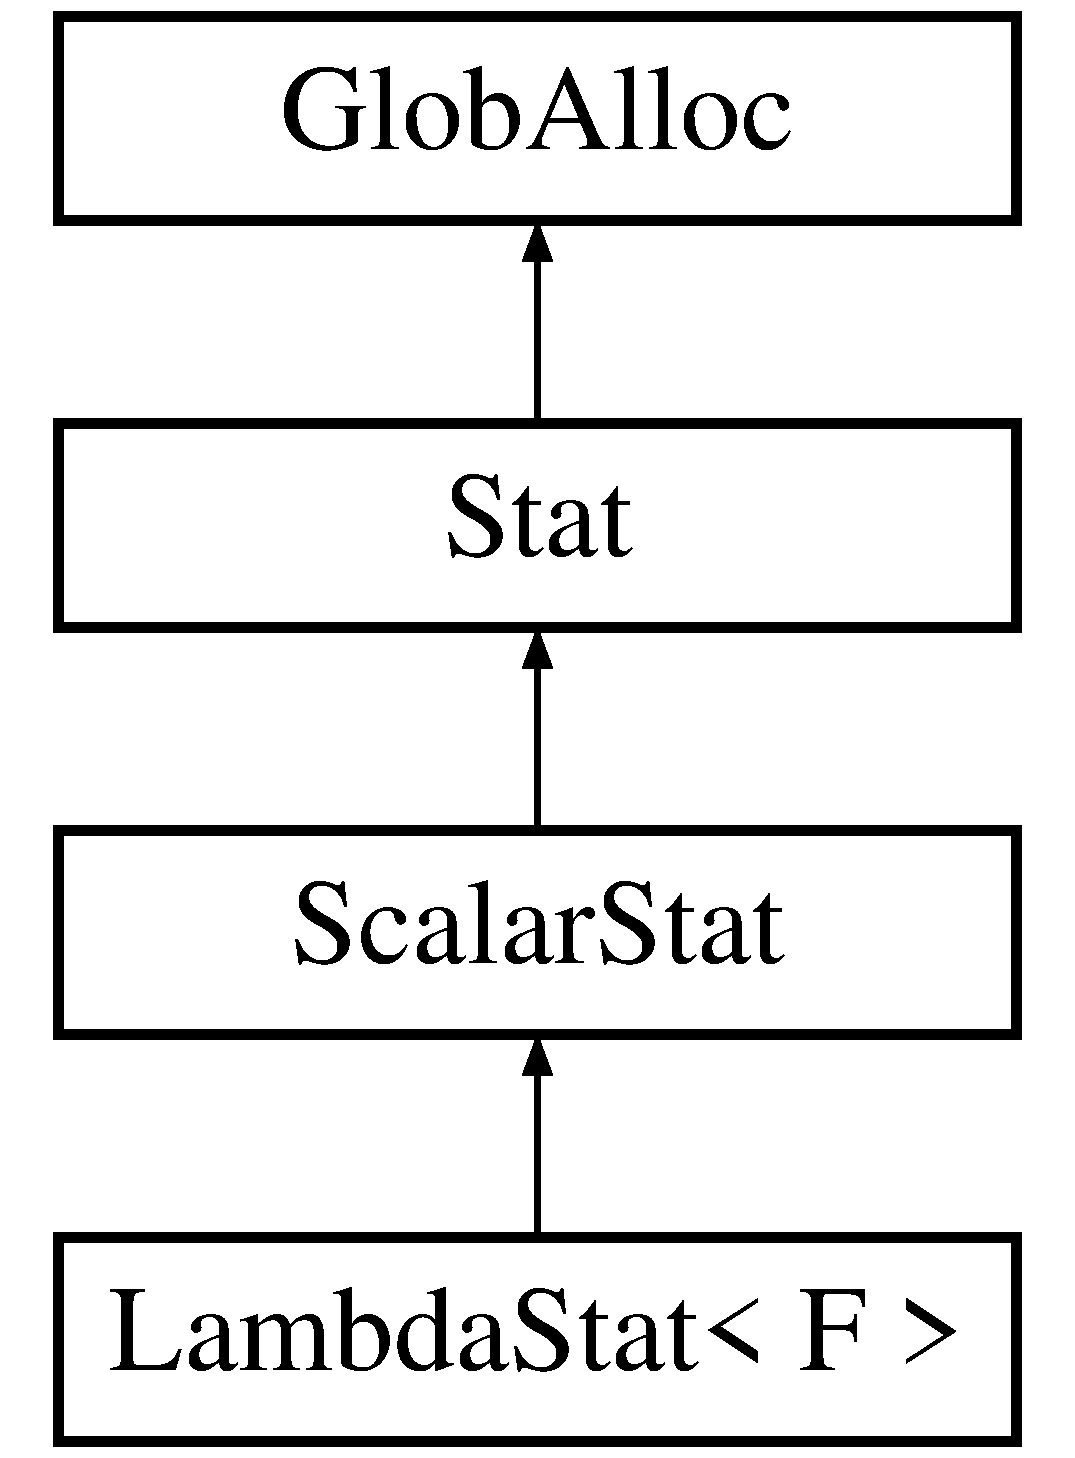
\includegraphics[height=4.000000cm]{classLambdaStat}
\end{center}
\end{figure}
\subsection*{Public Member Functions}
\begin{DoxyCompactItemize}
\item 
\hypertarget{classLambdaStat_a44cd3edc94f7eb6988cde776471162af}{{\bfseries Lambda\-Stat} (F \-\_\-f)}\label{classLambdaStat_a44cd3edc94f7eb6988cde776471162af}

\item 
\hypertarget{classLambdaStat_a2d4a7954b0b878035202182cb1b8d2db}{uint64\-\_\-t {\bfseries get} () const }\label{classLambdaStat_a2d4a7954b0b878035202182cb1b8d2db}

\end{DoxyCompactItemize}
\subsection*{Additional Inherited Members}


The documentation for this class was generated from the following file\-:\begin{DoxyCompactItemize}
\item 
stats.\-h\end{DoxyCompactItemize}

\hypertarget{classLambdaVectorStat}{\section{Lambda\-Vector\-Stat$<$ F $>$ Class Template Reference}
\label{classLambdaVectorStat}\index{Lambda\-Vector\-Stat$<$ F $>$@{Lambda\-Vector\-Stat$<$ F $>$}}
}
Inheritance diagram for Lambda\-Vector\-Stat$<$ F $>$\-:\begin{figure}[H]
\begin{center}
\leavevmode
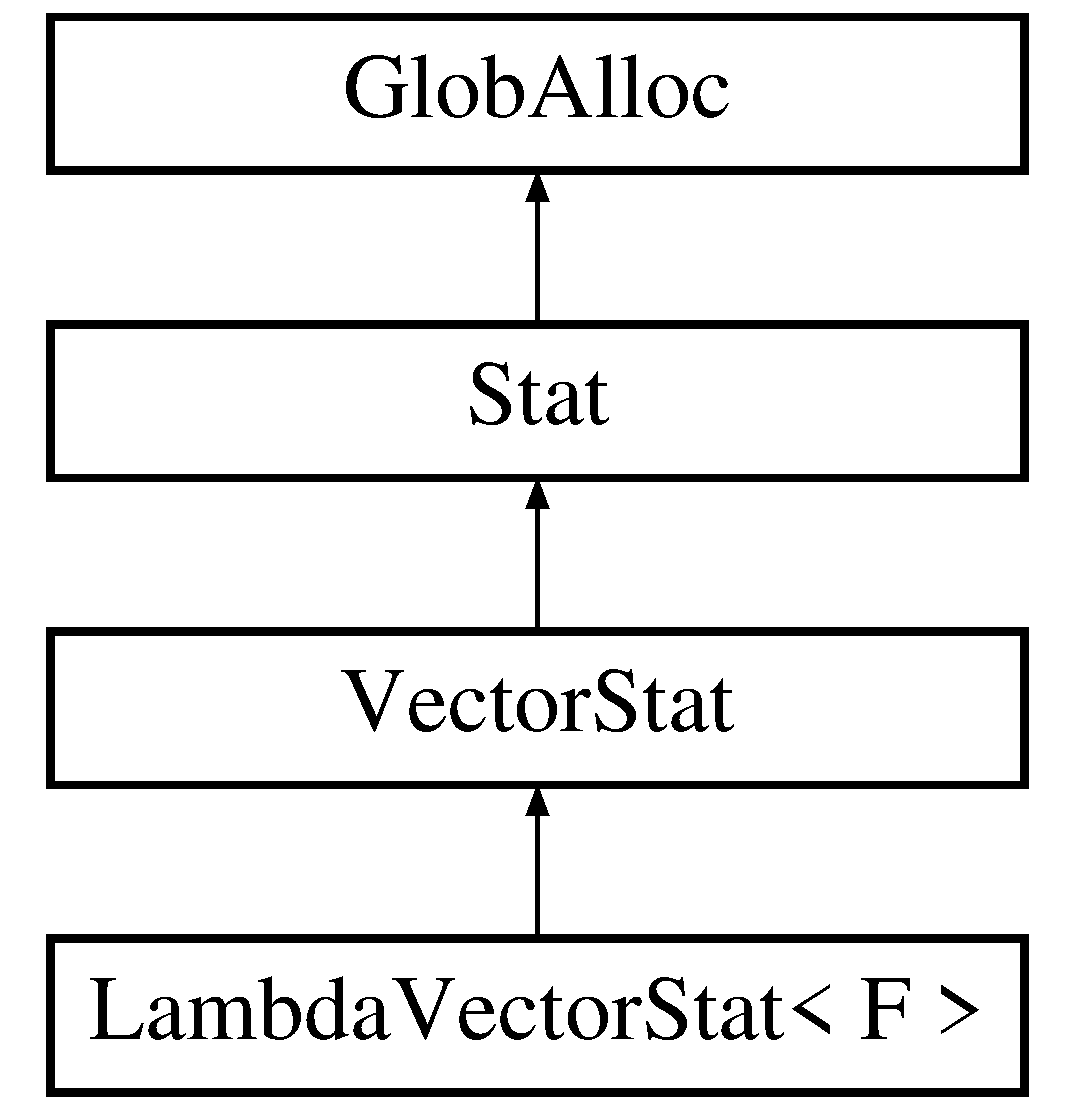
\includegraphics[height=4.000000cm]{classLambdaVectorStat}
\end{center}
\end{figure}
\subsection*{Public Member Functions}
\begin{DoxyCompactItemize}
\item 
\hypertarget{classLambdaVectorStat_a36d12c74f96d863725cb1b5b402e524b}{{\bfseries Lambda\-Vector\-Stat} (F \-\_\-f, uint32\-\_\-t \-\_\-s)}\label{classLambdaVectorStat_a36d12c74f96d863725cb1b5b402e524b}

\item 
\hypertarget{classLambdaVectorStat_a63e1c70625f3c350e59a99a7e2c94464}{uint32\-\_\-t {\bfseries size} () const }\label{classLambdaVectorStat_a63e1c70625f3c350e59a99a7e2c94464}

\item 
\hypertarget{classLambdaVectorStat_a7d53721746baf822cab7ecaffdc3cc0e}{uint64\-\_\-t {\bfseries count} (uint32\-\_\-t idx) const }\label{classLambdaVectorStat_a7d53721746baf822cab7ecaffdc3cc0e}

\end{DoxyCompactItemize}
\subsection*{Additional Inherited Members}


The documentation for this class was generated from the following file\-:\begin{DoxyCompactItemize}
\item 
stats.\-h\end{DoxyCompactItemize}

\hypertarget{classLegacyReplPolicy}{\section{Legacy\-Repl\-Policy Class Reference}
\label{classLegacyReplPolicy}\index{Legacy\-Repl\-Policy@{Legacy\-Repl\-Policy}}
}
Inheritance diagram for Legacy\-Repl\-Policy\-:\begin{figure}[H]
\begin{center}
\leavevmode
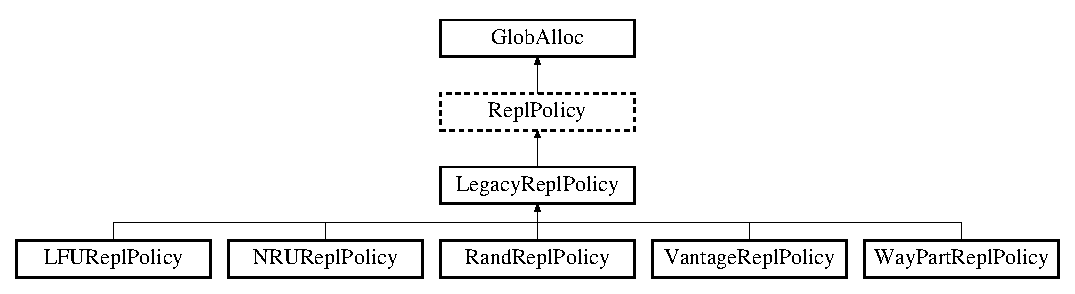
\includegraphics[height=3.500000cm]{classLegacyReplPolicy}
\end{center}
\end{figure}
\subsection*{Public Member Functions}
\begin{DoxyCompactItemize}
\item 
\hypertarget{classLegacyReplPolicy_a4614042323dae45191699811a093ab98}{{\footnotesize template$<$typename C $>$ }\\uint32\-\_\-t {\bfseries rank} (const \hyperlink{structMemReq}{Mem\-Req} $\ast$req, C cands)}\label{classLegacyReplPolicy_a4614042323dae45191699811a093ab98}

\end{DoxyCompactItemize}
\subsection*{Public Attributes}
\begin{DoxyCompactItemize}
\item 
\hypertarget{classLegacyReplPolicy_a78a3fe68b8dfe92cbd7d5b0d3c7b85a0}{{\bfseries D\-E\-C\-L\-\_\-\-R\-A\-N\-K\-\_\-\-B\-I\-N\-D\-I\-N\-G\-S}}\label{classLegacyReplPolicy_a78a3fe68b8dfe92cbd7d5b0d3c7b85a0}

\end{DoxyCompactItemize}
\subsection*{Protected Member Functions}
\begin{DoxyCompactItemize}
\item 
\hypertarget{classLegacyReplPolicy_a65938073835253f0fba77e821c1dbef0}{virtual void {\bfseries start\-Replacement} (const \hyperlink{structMemReq}{Mem\-Req} $\ast$req)}\label{classLegacyReplPolicy_a65938073835253f0fba77e821c1dbef0}

\item 
\hypertarget{classLegacyReplPolicy_ab1249dd2c85086076d8f666628c0322e}{virtual void {\bfseries record\-Candidate} (uint32\-\_\-t id)=0}\label{classLegacyReplPolicy_ab1249dd2c85086076d8f666628c0322e}

\item 
\hypertarget{classLegacyReplPolicy_a5fe3f005b39d8bba634f293aaf486572}{virtual uint32\-\_\-t {\bfseries get\-Best\-Candidate} ()=0}\label{classLegacyReplPolicy_a5fe3f005b39d8bba634f293aaf486572}

\end{DoxyCompactItemize}
\subsection*{Additional Inherited Members}


The documentation for this class was generated from the following file\-:\begin{DoxyCompactItemize}
\item 
repl\-\_\-policies.\-h\end{DoxyCompactItemize}

\hypertarget{classLFUReplPolicy}{\section{L\-F\-U\-Repl\-Policy Class Reference}
\label{classLFUReplPolicy}\index{L\-F\-U\-Repl\-Policy@{L\-F\-U\-Repl\-Policy}}
}
Inheritance diagram for L\-F\-U\-Repl\-Policy\-:\begin{figure}[H]
\begin{center}
\leavevmode
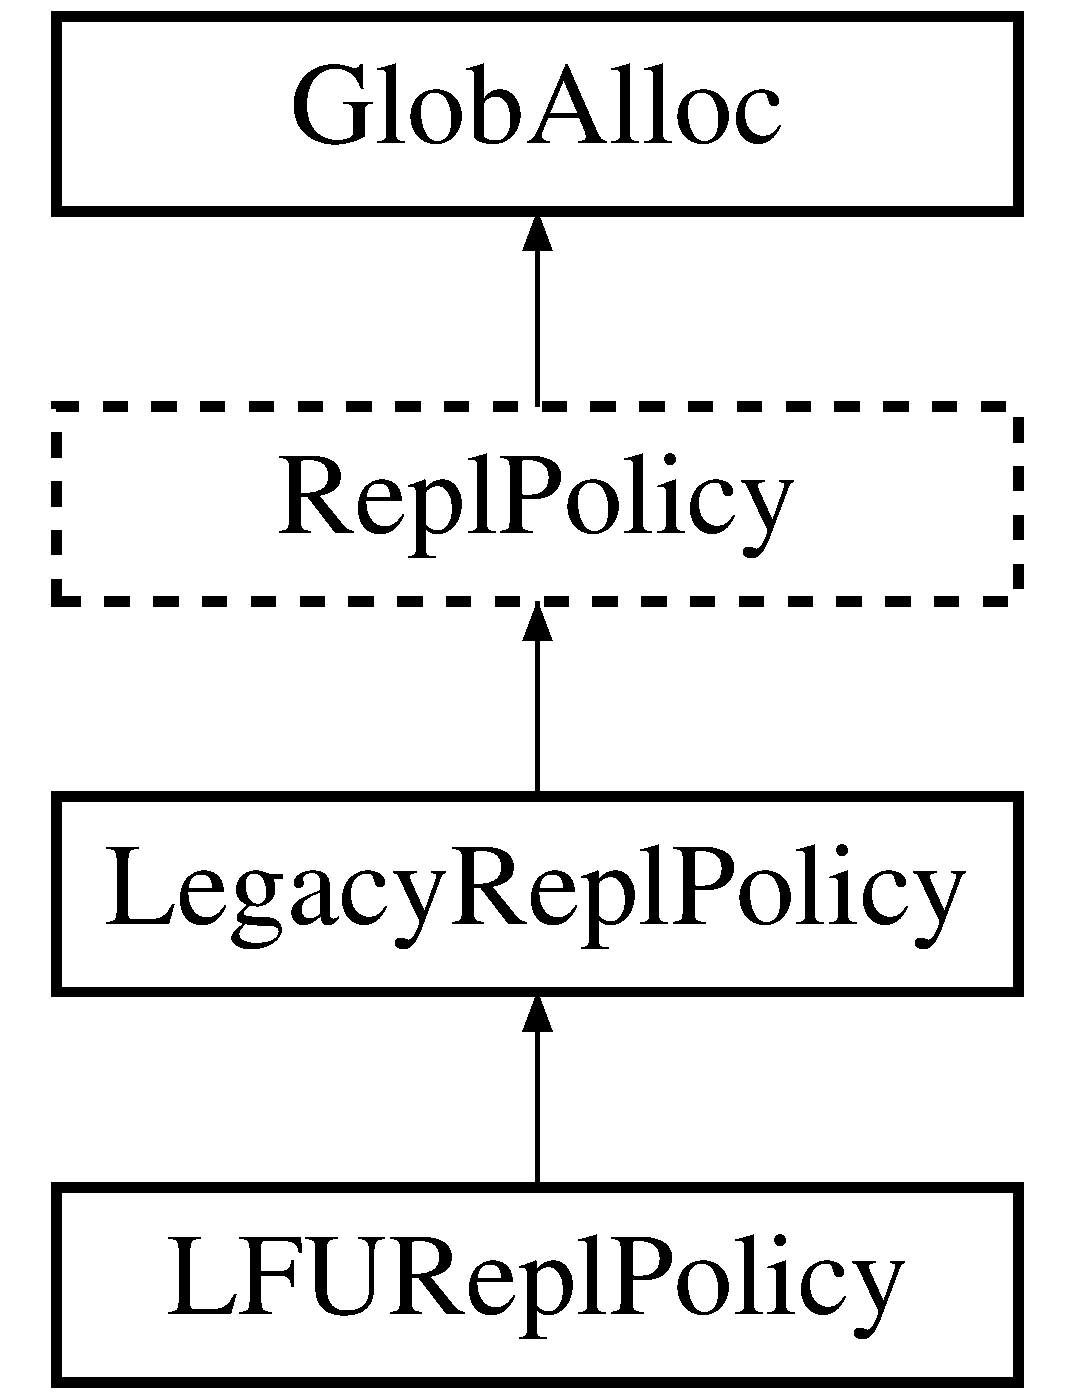
\includegraphics[height=4.000000cm]{classLFUReplPolicy}
\end{center}
\end{figure}
\subsection*{Public Member Functions}
\begin{DoxyCompactItemize}
\item 
\hypertarget{classLFUReplPolicy_a68506220223f68f0e1eb21c957b3ad94}{{\bfseries L\-F\-U\-Repl\-Policy} (uint32\-\_\-t \-\_\-num\-Lines)}\label{classLFUReplPolicy_a68506220223f68f0e1eb21c957b3ad94}

\item 
\hypertarget{classLFUReplPolicy_a50c8903887a1f03cb8cfb80e66ac7b6c}{void {\bfseries update} (uint32\-\_\-t id, const \hyperlink{structMemReq}{Mem\-Req} $\ast$req)}\label{classLFUReplPolicy_a50c8903887a1f03cb8cfb80e66ac7b6c}

\item 
\hypertarget{classLFUReplPolicy_a28c029e034077ddf59962c44e7c30533}{void {\bfseries record\-Candidate} (uint32\-\_\-t id)}\label{classLFUReplPolicy_a28c029e034077ddf59962c44e7c30533}

\item 
\hypertarget{classLFUReplPolicy_ae9d269e859d7cf85fdec6a070e4d4eb8}{uint32\-\_\-t {\bfseries get\-Best\-Candidate} ()}\label{classLFUReplPolicy_ae9d269e859d7cf85fdec6a070e4d4eb8}

\item 
\hypertarget{classLFUReplPolicy_aee2c951c5ea5d9f855466cbfef1f46bf}{void {\bfseries replaced} (uint32\-\_\-t id)}\label{classLFUReplPolicy_aee2c951c5ea5d9f855466cbfef1f46bf}

\end{DoxyCompactItemize}
\subsection*{Additional Inherited Members}


The documentation for this class was generated from the following file\-:\begin{DoxyCompactItemize}
\item 
repl\-\_\-policies.\-h\end{DoxyCompactItemize}

\hypertarget{structLibInfo}{\section{Lib\-Info Struct Reference}
\label{structLibInfo}\index{Lib\-Info@{Lib\-Info}}
}


{\ttfamily \#include $<$debug.\-h$>$}

\subsection*{Public Attributes}
\begin{DoxyCompactItemize}
\item 
\hypertarget{structLibInfo_a573bbdcfaf29366ef16a9ee9cf77ba82}{void $\ast$ {\bfseries text\-Addr}}\label{structLibInfo_a573bbdcfaf29366ef16a9ee9cf77ba82}

\item 
\hypertarget{structLibInfo_ab293b6055f594c556480666cf19dfddb}{void $\ast$ {\bfseries bss\-Addr}}\label{structLibInfo_ab293b6055f594c556480666cf19dfddb}

\item 
\hypertarget{structLibInfo_a0cec672450c8112cca9690af21dcad28}{void $\ast$ {\bfseries data\-Addr}}\label{structLibInfo_a0cec672450c8112cca9690af21dcad28}

\end{DoxyCompactItemize}


\subsection{Detailed Description}
\$lic\$ Copyright (C) 2012-\/2015 by Massachusetts Institute of Technology Copyright (C) 2010-\/2013 by The Board of Trustees of Stanford University

This file is part of zsim.

zsim is free software; you can redistribute it and/or modify it under the terms of the G\-N\-U General Public License as published by the Free Software Foundation, version 2.

If you use this software in your research, we request that you reference the zsim paper (\char`\"{}\-Z\-Sim\-: Fast and Accurate Microarchitectural Simulation of
\-Thousand-\/\-Core Systems\char`\"{}, Sanchez and Kozyrakis, I\-S\-C\-A-\/40, June 2013) as the source of the simulator in any publications that use this software, and that you send us a citation of your work.

zsim is distributed in the hope that it will be useful, but W\-I\-T\-H\-O\-U\-T A\-N\-Y W\-A\-R\-R\-A\-N\-T\-Y; without even the implied warranty of M\-E\-R\-C\-H\-A\-N\-T\-A\-B\-I\-L\-I\-T\-Y or F\-I\-T\-N\-E\-S\-S F\-O\-R A P\-A\-R\-T\-I\-C\-U\-L\-A\-R P\-U\-R\-P\-O\-S\-E. See the G\-N\-U General Public License for more details.

You should have received a copy of the G\-N\-U General Public License along with this program. If not, see \href{http://www.gnu.org/licenses/}{\tt http\-://www.\-gnu.\-org/licenses/}. 

The documentation for this struct was generated from the following file\-:\begin{DoxyCompactItemize}
\item 
debug.\-h\end{DoxyCompactItemize}

\hypertarget{classLinePlacementPolicy}{\section{Line\-Placement\-Policy Class Reference}
\label{classLinePlacementPolicy}\index{Line\-Placement\-Policy@{Line\-Placement\-Policy}}
}
\subsection*{Public Member Functions}
\begin{DoxyCompactItemize}
\item 
\hypertarget{classLinePlacementPolicy_a1126cfedae959b5731be05b098db344a}{void {\bfseries initialize} (\hyperlink{classConfig}{Config} \&config)}\label{classLinePlacementPolicy_a1126cfedae959b5731be05b098db344a}

\item 
\hypertarget{classLinePlacementPolicy_a13d6dad984a1bcebde7a771b6997024e}{bool {\bfseries handle\-Cache\-Miss} (\hyperlink{classWay}{Way} $\ast$current\-\_\-tad)}\label{classLinePlacementPolicy_a13d6dad984a1bcebde7a771b6997024e}

\end{DoxyCompactItemize}


The documentation for this class was generated from the following files\-:\begin{DoxyCompactItemize}
\item 
line\-\_\-placement.\-h\item 
line\-\_\-placement.\-cpp\end{DoxyCompactItemize}

\hypertarget{classLookaheadPartitioner}{\section{Lookahead\-Partitioner Class Reference}
\label{classLookaheadPartitioner}\index{Lookahead\-Partitioner@{Lookahead\-Partitioner}}
}
Inheritance diagram for Lookahead\-Partitioner\-:\begin{figure}[H]
\begin{center}
\leavevmode
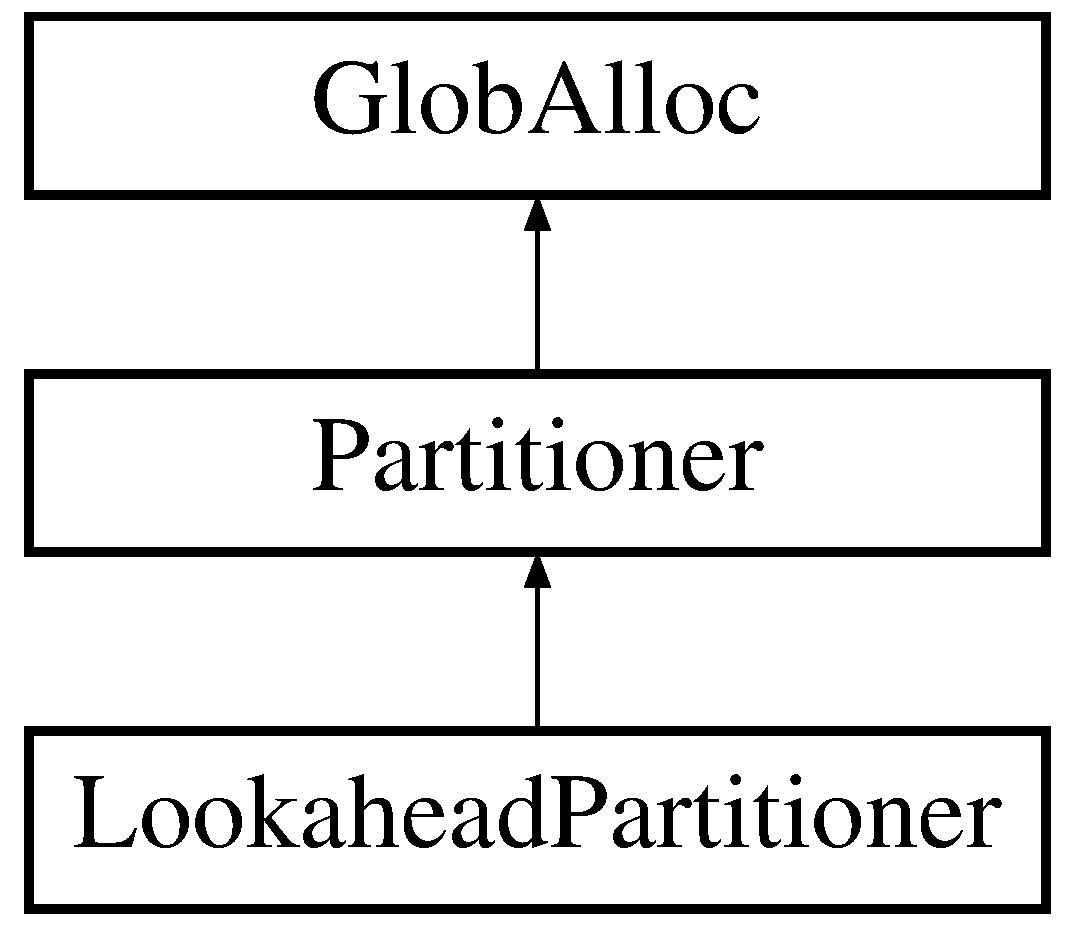
\includegraphics[height=3.000000cm]{classLookaheadPartitioner}
\end{center}
\end{figure}
\subsection*{Public Member Functions}
\begin{DoxyCompactItemize}
\item 
\hypertarget{classLookaheadPartitioner_a6f9409d5526f47560f6de4769911b97c}{{\bfseries Lookahead\-Partitioner} (\hyperlink{classPartReplPolicy}{Part\-Repl\-Policy} $\ast$\-\_\-repl, uint32\-\_\-t \-\_\-num\-Partitions, uint32\-\_\-t \-\_\-buckets, uint32\-\_\-t \-\_\-min\-Alloc=1, double \-\_\-alloc\-Portion=1.\-0, bool $\ast$\-\_\-forbidden=nullptr)}\label{classLookaheadPartitioner_a6f9409d5526f47560f6de4769911b97c}

\item 
\hypertarget{classLookaheadPartitioner_a205ac8b11251aea1baaf90f1399d33f3}{void {\bfseries partition} ()}\label{classLookaheadPartitioner_a205ac8b11251aea1baaf90f1399d33f3}

\end{DoxyCompactItemize}
\subsection*{Additional Inherited Members}


The documentation for this class was generated from the following files\-:\begin{DoxyCompactItemize}
\item 
partitioner.\-h\item 
lookahead.\-cpp\end{DoxyCompactItemize}

\hypertarget{classLRUReplPolicy}{\section{L\-R\-U\-Repl\-Policy$<$ sharers\-Aware $>$ Class Template Reference}
\label{classLRUReplPolicy}\index{L\-R\-U\-Repl\-Policy$<$ sharers\-Aware $>$@{L\-R\-U\-Repl\-Policy$<$ sharers\-Aware $>$}}
}
Inheritance diagram for L\-R\-U\-Repl\-Policy$<$ sharers\-Aware $>$\-:\begin{figure}[H]
\begin{center}
\leavevmode
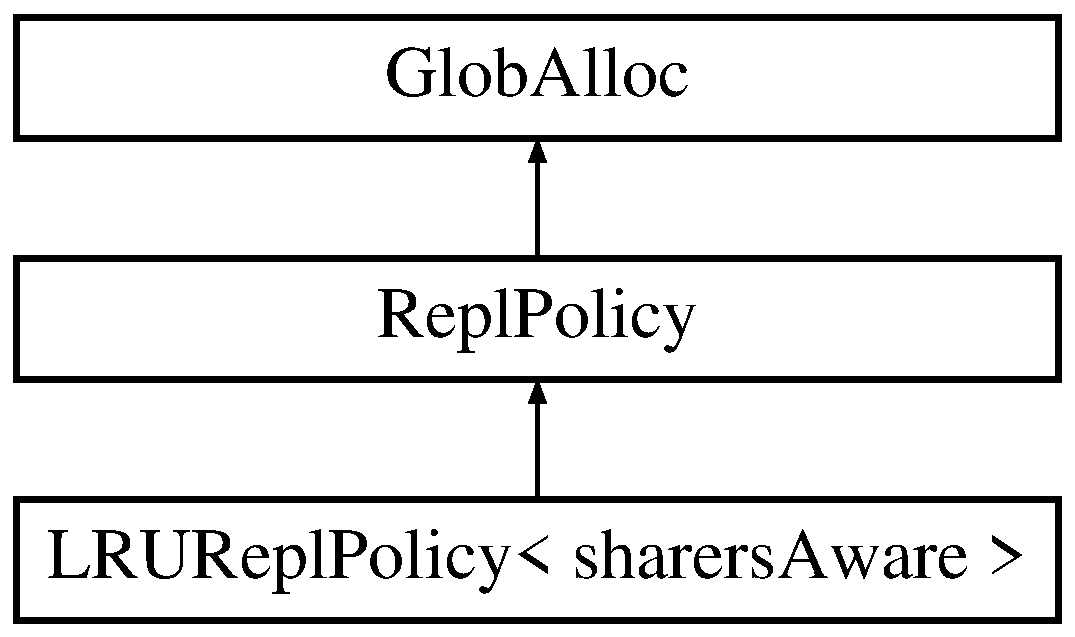
\includegraphics[height=3.000000cm]{classLRUReplPolicy}
\end{center}
\end{figure}
\subsection*{Public Member Functions}
\begin{DoxyCompactItemize}
\item 
\hypertarget{classLRUReplPolicy_a5b56dfdf924617f38a9ce0c40eee4531}{{\bfseries L\-R\-U\-Repl\-Policy} (uint32\-\_\-t \-\_\-num\-Lines)}\label{classLRUReplPolicy_a5b56dfdf924617f38a9ce0c40eee4531}

\item 
\hypertarget{classLRUReplPolicy_a8f0aaeb531fb610a3411b986904de164}{void {\bfseries update} (uint32\-\_\-t id, const \hyperlink{structMemReq}{Mem\-Req} $\ast$req)}\label{classLRUReplPolicy_a8f0aaeb531fb610a3411b986904de164}

\item 
\hypertarget{classLRUReplPolicy_a86764b8fbec69f372916587021fc03e0}{void {\bfseries replaced} (uint32\-\_\-t id)}\label{classLRUReplPolicy_a86764b8fbec69f372916587021fc03e0}

\item 
\hypertarget{classLRUReplPolicy_a1fc2a785e3066a2f6aa1a19c13451f8e}{{\footnotesize template$<$typename C $>$ }\\uint32\-\_\-t {\bfseries rank} (const \hyperlink{structMemReq}{Mem\-Req} $\ast$req, C cands)}\label{classLRUReplPolicy_a1fc2a785e3066a2f6aa1a19c13451f8e}

\end{DoxyCompactItemize}
\subsection*{Public Attributes}
\begin{DoxyCompactItemize}
\item 
\hypertarget{classLRUReplPolicy_a5ccee6aca3822b36fe38b89c3ce198b7}{{\bfseries D\-E\-C\-L\-\_\-\-R\-A\-N\-K\-\_\-\-B\-I\-N\-D\-I\-N\-G\-S}}\label{classLRUReplPolicy_a5ccee6aca3822b36fe38b89c3ce198b7}

\end{DoxyCompactItemize}
\subsection*{Protected Attributes}
\begin{DoxyCompactItemize}
\item 
\hypertarget{classLRUReplPolicy_a65b4e89421966a1190dbff428fc5ea06}{uint64\-\_\-t {\bfseries timestamp}}\label{classLRUReplPolicy_a65b4e89421966a1190dbff428fc5ea06}

\item 
\hypertarget{classLRUReplPolicy_a352504fa2cf1d16cd51d3c27d88dc32f}{uint64\-\_\-t $\ast$ {\bfseries array}}\label{classLRUReplPolicy_a352504fa2cf1d16cd51d3c27d88dc32f}

\item 
\hypertarget{classLRUReplPolicy_a1390ad4fdead8484451baebc26d1bdfb}{uint32\-\_\-t {\bfseries num\-Lines}}\label{classLRUReplPolicy_a1390ad4fdead8484451baebc26d1bdfb}

\end{DoxyCompactItemize}


The documentation for this class was generated from the following file\-:\begin{DoxyCompactItemize}
\item 
repl\-\_\-policies.\-h\end{DoxyCompactItemize}

\hypertarget{classMD1Memory}{\section{M\-D1\-Memory Class Reference}
\label{classMD1Memory}\index{M\-D1\-Memory@{M\-D1\-Memory}}
}
Inheritance diagram for M\-D1\-Memory\-:\begin{figure}[H]
\begin{center}
\leavevmode
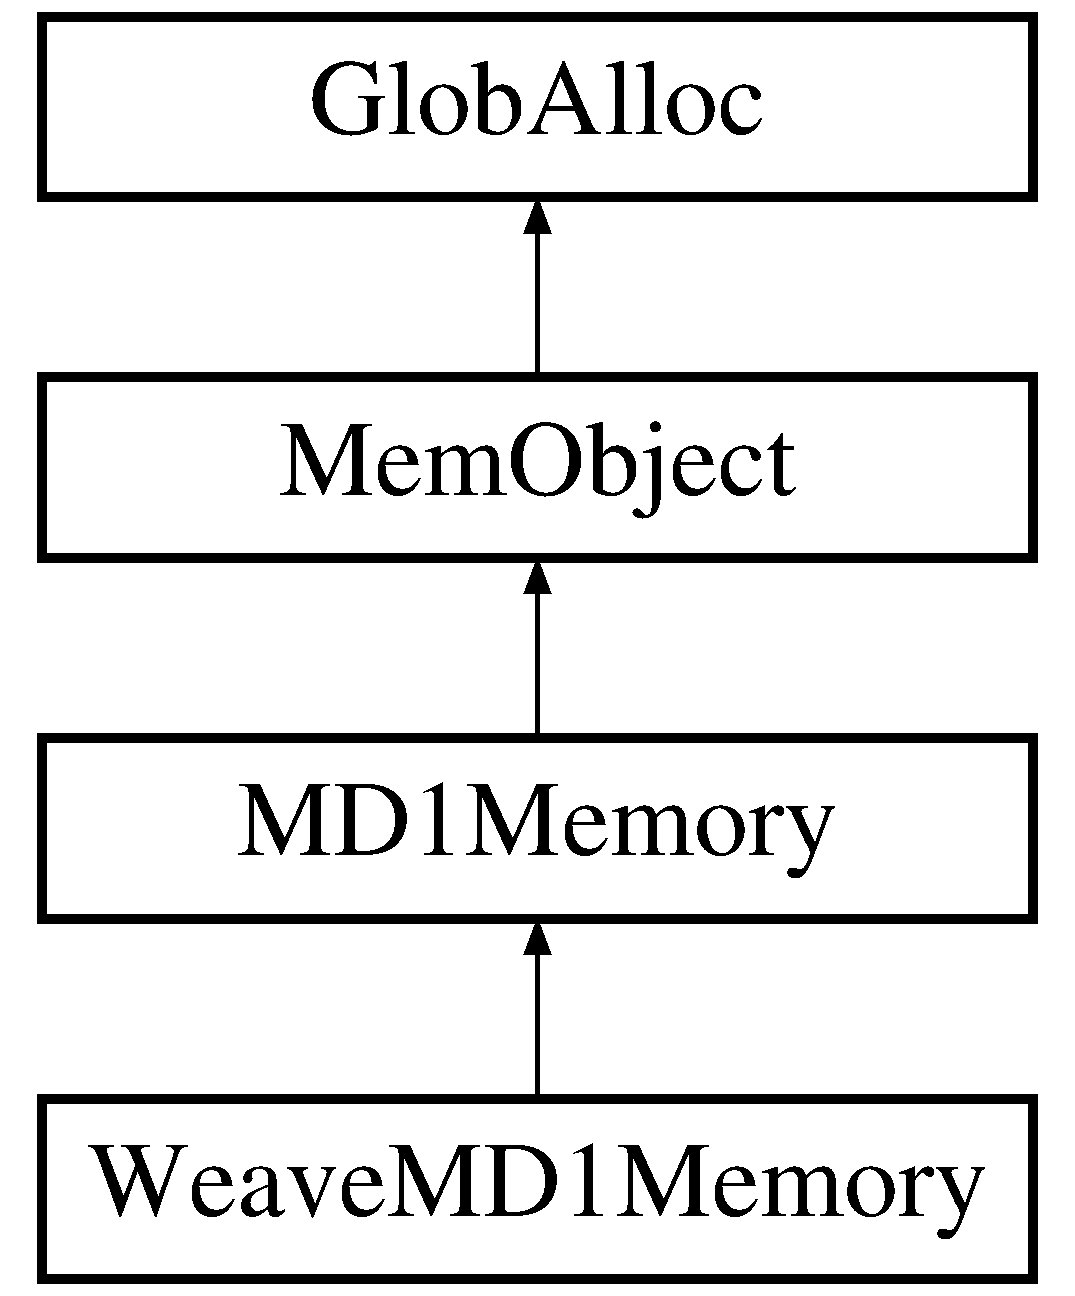
\includegraphics[height=4.000000cm]{classMD1Memory}
\end{center}
\end{figure}
\subsection*{Public Member Functions}
\begin{DoxyCompactItemize}
\item 
\hypertarget{classMD1Memory_a4664fc1ade5df44b4f6863e6f0cbf2f6}{{\bfseries M\-D1\-Memory} (uint32\-\_\-t line\-Size, uint32\-\_\-t megacycles\-Per\-Second, uint32\-\_\-t megabytes\-Per\-Second, uint32\-\_\-t \-\_\-zero\-Load\-Latency, g\-\_\-string \&\-\_\-name)}\label{classMD1Memory_a4664fc1ade5df44b4f6863e6f0cbf2f6}

\item 
\hypertarget{classMD1Memory_a657b4c85996c3ae5c88e481abc616bfe}{void {\bfseries init\-Stats} (\hyperlink{classAggregateStat}{Aggregate\-Stat} $\ast$parent\-Stat)}\label{classMD1Memory_a657b4c85996c3ae5c88e481abc616bfe}

\item 
\hypertarget{classMD1Memory_a75f00e592cf0c3feca3c01c1e9f0fd6c}{uint64\-\_\-t {\bfseries access} (\hyperlink{structMemReq}{Mem\-Req} \&req)}\label{classMD1Memory_a75f00e592cf0c3feca3c01c1e9f0fd6c}

\item 
\hypertarget{classMD1Memory_a26ccb0547e5840c22ada8b9cfc418464}{const char $\ast$ {\bfseries get\-Name} ()}\label{classMD1Memory_a26ccb0547e5840c22ada8b9cfc418464}

\end{DoxyCompactItemize}


The documentation for this class was generated from the following files\-:\begin{DoxyCompactItemize}
\item 
mem\-\_\-ctrls.\-h\item 
mem\-\_\-ctrls.\-cpp\end{DoxyCompactItemize}

\hypertarget{classMemAccessEventBase}{\section{Mem\-Access\-Event\-Base Class Reference}
\label{classMemAccessEventBase}\index{Mem\-Access\-Event\-Base@{Mem\-Access\-Event\-Base}}
}
Inheritance diagram for Mem\-Access\-Event\-Base\-:\begin{figure}[H]
\begin{center}
\leavevmode
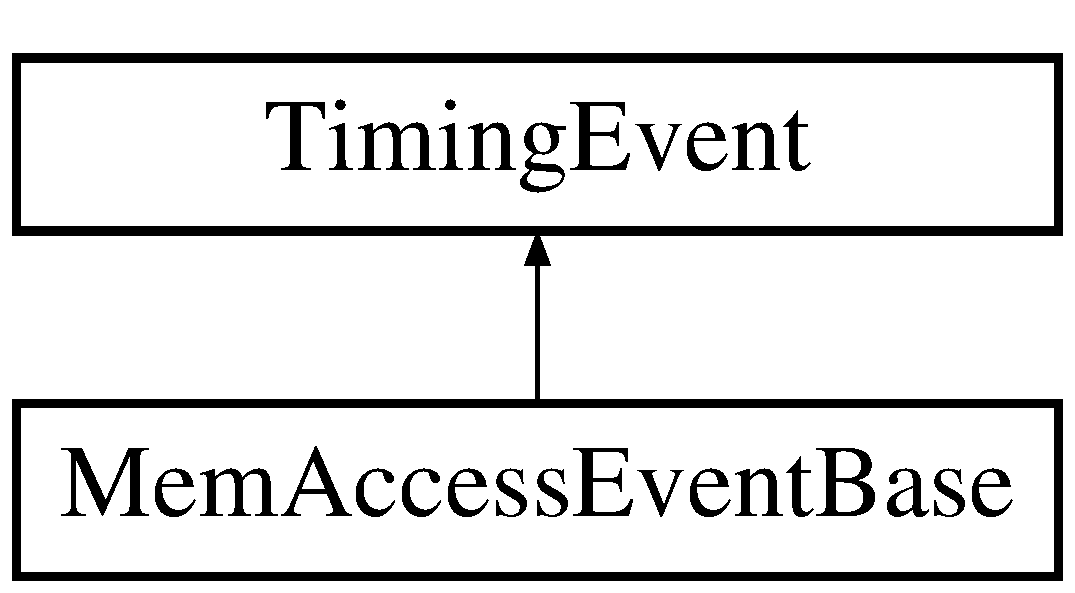
\includegraphics[height=2.000000cm]{classMemAccessEventBase}
\end{center}
\end{figure}
\subsection*{Public Member Functions}
\begin{DoxyCompactItemize}
\item 
\hypertarget{classMemAccessEventBase_abc754afb4dad414c2e41cb6a78a28783}{{\bfseries Mem\-Access\-Event\-Base} (\hyperlink{classMemControllerBase}{Mem\-Controller\-Base} $\ast$\-\_\-dram, Mem\-Access\-Type \-\_\-type, Address \-\_\-addr, int32\-\_\-t domain, uint32\-\_\-t pre\-Delay, uint32\-\_\-t post\-Delay)}\label{classMemAccessEventBase_abc754afb4dad414c2e41cb6a78a28783}

\item 
\hypertarget{classMemAccessEventBase_a5ef5c4322e608e54eed1930855333f80}{void {\bfseries simulate} (uint64\-\_\-t start\-Cycle)}\label{classMemAccessEventBase_a5ef5c4322e608e54eed1930855333f80}

\item 
\hypertarget{classMemAccessEventBase_ac85f64b8558421bf47cb7a60e990ff17}{Mem\-Access\-Type {\bfseries get\-Type} () const }\label{classMemAccessEventBase_ac85f64b8558421bf47cb7a60e990ff17}

\item 
\hypertarget{classMemAccessEventBase_a9cc9d17bda3a19800a4f11e7e2891632}{Address {\bfseries get\-Addr} () const }\label{classMemAccessEventBase_a9cc9d17bda3a19800a4f11e7e2891632}

\end{DoxyCompactItemize}
\subsection*{Additional Inherited Members}


The documentation for this class was generated from the following file\-:\begin{DoxyCompactItemize}
\item 
detailed\-\_\-mem.\-h\end{DoxyCompactItemize}

\hypertarget{classMemChannelBase}{\section{Mem\-Channel\-Base Class Reference}
\label{classMemChannelBase}\index{Mem\-Channel\-Base@{Mem\-Channel\-Base}}
}
Inheritance diagram for Mem\-Channel\-Base\-:\begin{figure}[H]
\begin{center}
\leavevmode
\includegraphics[height=2.000000cm]{classMemChannelBase}
\end{center}
\end{figure}
\subsection*{Public Member Functions}
\begin{DoxyCompactItemize}
\item 
\hypertarget{classMemChannelBase_a2e476e5df6a1f1a2af74176f5f430780}{{\bfseries Mem\-Channel\-Base} (uint32\-\_\-t \-\_\-my\-Id, \hyperlink{classMemParam}{Mem\-Param} $\ast$\-\_\-m\-Param)}\label{classMemChannelBase_a2e476e5df6a1f1a2af74176f5f430780}

\item 
\hypertarget{classMemChannelBase_a5fb78770709c769c6d0f360420b7ff3c}{virtual uint64\-\_\-t {\bfseries Latency\-Simulate} (Address line\-Addr, uint64\-\_\-t arrival\-Cycle, uint64\-\_\-t last\-Phase\-Cycle, Mem\-Access\-Type type)}\label{classMemChannelBase_a5fb78770709c769c6d0f360420b7ff3c}

\item 
\hypertarget{classMemChannelBase_a48733e49e1666216025e1881f4fa061e}{virtual void {\bfseries Address\-Map} (Address addr, uint32\-\_\-t \&row, uint32\-\_\-t \&col, uint32\-\_\-t \&rank, uint32\-\_\-t \&bank)}\label{classMemChannelBase_a48733e49e1666216025e1881f4fa061e}

\item 
\hypertarget{classMemChannelBase_a7e37609da4d99dcf76b94e85e76d6f3d}{bool {\bfseries Is\-Row\-Buffer\-Hit} (uint32\-\_\-t row, uint32\-\_\-t rank, uint32\-\_\-t bank)}\label{classMemChannelBase_a7e37609da4d99dcf76b94e85e76d6f3d}

\item 
\hypertarget{classMemChannelBase_a20d5444e086ec2ecb502eeb2bcf198ca}{virtual uint64\-\_\-t {\bfseries Get\-Activate\-Count} (void)}\label{classMemChannelBase_a20d5444e086ec2ecb502eeb2bcf198ca}

\item 
\hypertarget{classMemChannelBase_a42edfd2e48dc62f4736ad0fb341673ea}{virtual uint64\-\_\-t {\bfseries Get\-Precharge\-Count} (void)}\label{classMemChannelBase_a42edfd2e48dc62f4736ad0fb341673ea}

\item 
\hypertarget{classMemChannelBase_af57764a13bc54314580b76f93b36e06e}{virtual uint64\-\_\-t {\bfseries Get\-Refresh\-Count} (void)}\label{classMemChannelBase_af57764a13bc54314580b76f93b36e06e}

\item 
\hypertarget{classMemChannelBase_ac4fe84eb254e133f47708a32c9a86c01}{virtual uint64\-\_\-t {\bfseries Get\-Burst\-Energy} (void)}\label{classMemChannelBase_ac4fe84eb254e133f47708a32c9a86c01}

\item 
\hypertarget{classMemChannelBase_acc0b3c449b8510255366da62f21b32a2}{virtual uint64\-\_\-t {\bfseries Get\-Act\-Pre\-Energy} (void)}\label{classMemChannelBase_acc0b3c449b8510255366da62f21b32a2}

\item 
\hypertarget{classMemChannelBase_a380b6b65ddbc0de0d9bb3ecc199d85c0}{virtual uint64\-\_\-t {\bfseries Get\-Refresh\-Energy} (void)}\label{classMemChannelBase_a380b6b65ddbc0de0d9bb3ecc199d85c0}

\item 
\hypertarget{classMemChannelBase_a9c734e2143117c54de9f98054dad2ca7}{virtual uint64\-\_\-t {\bfseries Get\-Back\-Ground\-Energy} (uint64\-\_\-t mem\-Cycle, uint64\-\_\-t last\-Mem\-Cycle, bool b\-Instant=false)}\label{classMemChannelBase_a9c734e2143117c54de9f98054dad2ca7}

\item 
\hypertarget{classMemChannelBase_a796fe1cfd947821d2127f1b2acd1541f}{virtual void {\bfseries Periodic\-Update\-Power} (uint64\-\_\-t phase\-Cycle, uint64\-\_\-t last\-Phase\-Cycle)}\label{classMemChannelBase_a796fe1cfd947821d2127f1b2acd1541f}

\end{DoxyCompactItemize}
\subsection*{Protected Member Functions}
\begin{DoxyCompactItemize}
\item 
\hypertarget{classMemChannelBase_afcd52ed68d557269656f7a924439d8da}{virtual uint32\-\_\-t {\bfseries Update\-Refresh\-Num} (uint32\-\_\-t rank, uint64\-\_\-t arrival\-Cycle)}\label{classMemChannelBase_afcd52ed68d557269656f7a924439d8da}

\item 
\hypertarget{classMemChannelBase_afe808ac3c91971d3ca2c6abc102a74b4}{virtual uint64\-\_\-t {\bfseries Update\-Last\-Refresh\-Cycle} (uint32\-\_\-t rank, uint64\-\_\-t arrival\-Cycle, uint32\-\_\-t refresh\-Num)}\label{classMemChannelBase_afe808ac3c91971d3ca2c6abc102a74b4}

\item 
\hypertarget{classMemChannelBase_afb623d60de5b36bebb39d9e21827f6e8}{virtual void {\bfseries Update\-Power\-Down\-Cycle} (uint32\-\_\-t rank, uint64\-\_\-t arrival\-Cycle, uint64\-\_\-t last\-Phase\-Cycle, uint32\-\_\-t refresh\-Num)}\label{classMemChannelBase_afb623d60de5b36bebb39d9e21827f6e8}

\item 
\hypertarget{classMemChannelBase_aeb0400d262f6c664792449f8253e05ba}{virtual void {\bfseries Update\-Data\-Bus\-Cycle} (uint64\-\_\-t start, uint64\-\_\-t end)}\label{classMemChannelBase_aeb0400d262f6c664792449f8253e05ba}

\item 
\hypertarget{classMemChannelBase_ac93aad272161b449246548a4e273431d}{virtual void {\bfseries Issue\-Activate} (uint32\-\_\-t rank, uint32\-\_\-t bank, uint64\-\_\-t issued\-Cycle)}\label{classMemChannelBase_ac93aad272161b449246548a4e273431d}

\item 
\hypertarget{classMemChannelBase_af92d30734305756e52a9b2e2b2b6bf0c}{virtual void {\bfseries Issue\-Precharge} (uint32\-\_\-t rank, uint32\-\_\-t bank, uint64\-\_\-t issued\-Cycle, bool continuous=false)}\label{classMemChannelBase_af92d30734305756e52a9b2e2b2b6bf0c}

\item 
\hypertarget{classMemChannelBase_afb3cbd4a7c94e0e864405e400b89d4b1}{virtual uint64\-\_\-t {\bfseries Calc\-Intra\-Issue\-Cycle} (bool row\-Hit, uint32\-\_\-t rank, Mem\-Access\-Type type, uint64\-\_\-t arrival\-Cycle, uint32\-\_\-t refresh\-Num)}\label{classMemChannelBase_afb3cbd4a7c94e0e864405e400b89d4b1}

\item 
\hypertarget{classMemChannelBase_a004618cbad63872b77f73fb46507ae88}{virtual uint64\-\_\-t {\bfseries Calc\-Inter\-Issue\-Cycle} (Mem\-Access\-Type type, uint64\-\_\-t arrival\-Cycle)}\label{classMemChannelBase_a004618cbad63872b77f73fb46507ae88}

\item 
\hypertarget{classMemChannelBase_a9808754c103a7cb6700d19176db56826}{virtual uint64\-\_\-t {\bfseries Calc\-Act\-Const} (uint32\-\_\-t rank, uint32\-\_\-t bank, uint64\-\_\-t issuable\-Cycle)}\label{classMemChannelBase_a9808754c103a7cb6700d19176db56826}

\item 
\hypertarget{classMemChannelBase_aa3596a5a18c951ca3df722459589e7bd}{virtual uint64\-\_\-t {\bfseries Calc\-Pre\-Const} (uint32\-\_\-t rank, uint32\-\_\-t bank, Mem\-Access\-Type type, uint64\-\_\-t issuable\-Cycle)}\label{classMemChannelBase_aa3596a5a18c951ca3df722459589e7bd}

\item 
\hypertarget{classMemChannelBase_aabd0c4decaa154fca93cd7809cd5eae5}{virtual uint64\-\_\-t {\bfseries Calc\-Rd\-Wr\-Const} (uint32\-\_\-t rank, Mem\-Access\-Type type, uint64\-\_\-t issuable\-Cycle)}\label{classMemChannelBase_aabd0c4decaa154fca93cd7809cd5eae5}

\item 
\hypertarget{classMemChannelBase_a94f245dd5873c65df9b97901a7339e1f}{virtual uint32\-\_\-t {\bfseries Get\-Power\-Down\-Penalty} (uint32\-\_\-t rank, uint64\-\_\-t arrival\-Cycle)}\label{classMemChannelBase_a94f245dd5873c65df9b97901a7339e1f}

\item 
\hypertarget{classMemChannelBase_a3e58cb7900f1ee33c067f09285ef8e81}{virtual bool {\bfseries Check\-Continuous\-Access} (uint64\-\_\-t arrival\-Cycle, uint32\-\_\-t rank, uint32\-\_\-t bank, uint32\-\_\-t row)}\label{classMemChannelBase_a3e58cb7900f1ee33c067f09285ef8e81}

\end{DoxyCompactItemize}
\subsection*{Protected Attributes}
\begin{DoxyCompactItemize}
\item 
\hypertarget{classMemChannelBase_a7a8fb00f3696fe94d0481cae51ac465d}{uint32\-\_\-t {\bfseries my\-Id}}\label{classMemChannelBase_a7a8fb00f3696fe94d0481cae51ac465d}

\item 
\hypertarget{classMemChannelBase_ad7f8f8563be92ce36d94dbccf7ef1087}{\hyperlink{classMemParam}{Mem\-Param} $\ast$ {\bfseries m\-Param}}\label{classMemChannelBase_ad7f8f8563be92ce36d94dbccf7ef1087}

\item 
\hypertarget{classMemChannelBase_aaf66ca50858e84f178b4c8bd33906950}{\hyperlink{classg__vector}{g\-\_\-vector}$<$ \hyperlink{classMemRankBase}{Mem\-Rank\-Base} $\ast$ $>$ {\bfseries ranks}}\label{classMemChannelBase_aaf66ca50858e84f178b4c8bd33906950}

\item 
\hypertarget{classMemChannelBase_ac8d24b0f4f6f2aa7c0cb5f28e192f39d}{std\-::vector$<$ std\-::pair\\*
$<$ uint64\-\_\-t, uint64\-\_\-t $>$ $>$ {\bfseries access\-Log}}\label{classMemChannelBase_ac8d24b0f4f6f2aa7c0cb5f28e192f39d}

\end{DoxyCompactItemize}


The documentation for this class was generated from the following files\-:\begin{DoxyCompactItemize}
\item 
detailed\-\_\-mem.\-h\item 
detailed\-\_\-mem.\-cpp\end{DoxyCompactItemize}

\hypertarget{classMemControllerBase}{\section{Mem\-Controller\-Base Class Reference}
\label{classMemControllerBase}\index{Mem\-Controller\-Base@{Mem\-Controller\-Base}}
}
Inheritance diagram for Mem\-Controller\-Base\-:\begin{figure}[H]
\begin{center}
\leavevmode
\includegraphics[height=3.000000cm]{classMemControllerBase}
\end{center}
\end{figure}
\subsection*{Classes}
\begin{DoxyCompactItemize}
\item 
struct \hyperlink{structMemControllerBase_1_1powerValue}{power\-Value}
\end{DoxyCompactItemize}
\subsection*{Public Member Functions}
\begin{DoxyCompactItemize}
\item 
\hypertarget{classMemControllerBase_a3cb4e5c7ae504117be8c6ff15502dcc6}{{\bfseries Mem\-Controller\-Base} (g\-\_\-string \-\_\-mem\-Cfg, uint32\-\_\-t \-\_\-cache\-Line\-Size, uint32\-\_\-t \-\_\-sys\-Freq\-M\-Hz, uint32\-\_\-t \-\_\-domain, g\-\_\-string \&\-\_\-name)}\label{classMemControllerBase_a3cb4e5c7ae504117be8c6ff15502dcc6}

\item 
\hypertarget{classMemControllerBase_ac85a1504e9c0652e1612d59badde0032}{const char $\ast$ {\bfseries get\-Name} ()}\label{classMemControllerBase_ac85a1504e9c0652e1612d59badde0032}

\item 
\hypertarget{classMemControllerBase_a4cd70799a3c1edb0af291878f5a9a773}{void {\bfseries enqueue} (\hyperlink{classMemAccessEventBase}{Mem\-Access\-Event\-Base} $\ast$ev, uint64\-\_\-t cycle)}\label{classMemControllerBase_a4cd70799a3c1edb0af291878f5a9a773}

\item 
\hypertarget{classMemControllerBase_a5db8f1b19708c92ae85e3797bf6d6f8b}{uint64\-\_\-t {\bfseries access} (\hyperlink{structMemReq}{Mem\-Req} \&req)}\label{classMemControllerBase_a5db8f1b19708c92ae85e3797bf6d6f8b}

\item 
\hypertarget{classMemControllerBase_ac926fe00ab34f86ed5f2fb398668f978}{uint32\-\_\-t {\bfseries tick} (uint64\-\_\-t sys\-Cycle)}\label{classMemControllerBase_ac926fe00ab34f86ed5f2fb398668f978}

\item 
\hypertarget{classMemControllerBase_a9703e0e4f3b0846c3560f10f6e11492e}{void {\bfseries init\-Stats} (\hyperlink{classAggregateStat}{Aggregate\-Stat} $\ast$parent\-Stat)}\label{classMemControllerBase_a9703e0e4f3b0846c3560f10f6e11492e}

\item 
\hypertarget{classMemControllerBase_ab575ace5f9c765308ab6aa3ca64d5559}{void {\bfseries update\-Stats} (void)}\label{classMemControllerBase_ab575ace5f9c765308ab6aa3ca64d5559}

\item 
\hypertarget{classMemControllerBase_a4c23cd0fbf82abc036fa0050cf752d60}{void {\bfseries finish} (void)}\label{classMemControllerBase_a4c23cd0fbf82abc036fa0050cf752d60}

\end{DoxyCompactItemize}
\subsection*{Protected Member Functions}
\begin{DoxyCompactItemize}
\item 
\hypertarget{classMemControllerBase_a5876978d498a9419a1737f739ba9da57}{virtual uint64\-\_\-t {\bfseries Return\-Channel} (Address addr)}\label{classMemControllerBase_a5876978d498a9419a1737f739ba9da57}

\item 
\hypertarget{classMemControllerBase_ab8db0d9dad3b6636e4823fb6f27ec632}{virtual uint64\-\_\-t {\bfseries Latency\-Simulate} (Address line\-Addr, uint64\-\_\-t sys\-Cycle, Mem\-Access\-Type type)}\label{classMemControllerBase_ab8db0d9dad3b6636e4823fb6f27ec632}

\item 
\hypertarget{classMemControllerBase_aedd18f1b2a1f5e2996f3a63a2318b6e3}{virtual void {\bfseries Update\-Cmd\-Counters} (void)}\label{classMemControllerBase_aedd18f1b2a1f5e2996f3a63a2318b6e3}

\item 
\hypertarget{classMemControllerBase_a4839d77437ef24c9db6ac2cf00c1fb43}{virtual void {\bfseries Estimate\-Powers} (uint64\-\_\-t sys\-Cycle, bool finish=false)}\label{classMemControllerBase_a4839d77437ef24c9db6ac2cf00c1fb43}

\item 
\hypertarget{classMemControllerBase_a13d9efb4d902b74dd4b2deda7181906f}{virtual void {\bfseries Estimate\-Bandwidth} (uint64\-\_\-t real\-Time, uint64\-\_\-t last\-Time, bool finish=false)}\label{classMemControllerBase_a13d9efb4d902b74dd4b2deda7181906f}

\item 
\hypertarget{classMemControllerBase_a11fc2734502345a5a106a4626d64b418}{virtual uint64\-\_\-t {\bfseries Calc\-D\-Q\-Term\-Cur} (uint64\-\_\-t acc\-\_\-dq, uint64\-\_\-t last\-\_\-dq, uint64\-\_\-t inst\-Cycle, uint64\-\_\-t mem\-Cycle, uint64\-\_\-t last\-Mem\-Cycle)}\label{classMemControllerBase_a11fc2734502345a5a106a4626d64b418}

\item 
\hypertarget{classMemControllerBase_a2a4f871e47c0a60424db4f2e28b4aef7}{virtual uint64\-\_\-t {\bfseries Calc\-D\-Q\-Term\-Acc} (uint64\-\_\-t acc\-\_\-dq, uint64\-\_\-t mem\-Cycle, uint64\-\_\-t last\-Mem\-Cycle)}\label{classMemControllerBase_a2a4f871e47c0a60424db4f2e28b4aef7}

\item 
\hypertarget{classMemControllerBase_a2cd02ede21ab33ea364bd2ae14df35d9}{virtual void {\bfseries Tick\-Scheduler} (uint64\-\_\-t sys\-Cycle)}\label{classMemControllerBase_a2cd02ede21ab33ea364bd2ae14df35d9}

\item 
\hypertarget{classMemControllerBase_a7177fcd259a98335c3c32b1dc86c54f6}{uint64\-\_\-t {\bfseries sys\-To\-Mem\-Cycle} (uint64\-\_\-t sys\-Cycle)}\label{classMemControllerBase_a7177fcd259a98335c3c32b1dc86c54f6}

\item 
\hypertarget{classMemControllerBase_aa09dc5a73cb7437ff5aac88515e469e6}{uint64\-\_\-t {\bfseries sys\-To\-Micro\-Sec} (uint64\-\_\-t sys\-Cycle)}\label{classMemControllerBase_aa09dc5a73cb7437ff5aac88515e469e6}

\item 
\hypertarget{classMemControllerBase_aaf2fdcacf48b08800ffd1aabd8ac36b9}{uint64\-\_\-t {\bfseries usec\-To\-Sys\-Cycle} (uint64\-\_\-t usec)}\label{classMemControllerBase_aaf2fdcacf48b08800ffd1aabd8ac36b9}

\item 
\hypertarget{classMemControllerBase_aab7c0e55f63511b8ce54ec2d765115ad}{uint64\-\_\-t {\bfseries mem\-To\-Sys\-Cycle} (uint64\-\_\-t mem\-Cycle)}\label{classMemControllerBase_aab7c0e55f63511b8ce54ec2d765115ad}

\item 
\hypertarget{classMemControllerBase_a1516dc45607d418a6171562927486b08}{uint64\-\_\-t {\bfseries mem\-To\-Micro\-Sec} (uint64\-\_\-t mem\-Cycle)}\label{classMemControllerBase_a1516dc45607d418a6171562927486b08}

\end{DoxyCompactItemize}
\subsection*{Protected Attributes}
\begin{DoxyCompactItemize}
\item 
\hypertarget{classMemControllerBase_a365a95eafef280acf977109508e3822a}{g\-\_\-string {\bfseries name}}\label{classMemControllerBase_a365a95eafef280acf977109508e3822a}

\item 
\hypertarget{classMemControllerBase_aa53b4d80588c5b80992893d5b0a77290}{uint32\-\_\-t {\bfseries domain}}\label{classMemControllerBase_aa53b4d80588c5b80992893d5b0a77290}

\item 
\hypertarget{classMemControllerBase_aac8a82822840a4e9429177aad75a5bc0}{uint32\-\_\-t {\bfseries cache\-Line\-Size}}\label{classMemControllerBase_aac8a82822840a4e9429177aad75a5bc0}

\item 
\hypertarget{classMemControllerBase_a723ddecb498404f3ada20a85549da45c}{\hyperlink{classMemParam}{Mem\-Param} $\ast$ {\bfseries m\-Param}}\label{classMemControllerBase_a723ddecb498404f3ada20a85549da45c}

\item 
\hypertarget{classMemControllerBase_a3192c564283ff25cf0a071b0f0070806}{\hyperlink{classg__vector}{g\-\_\-vector}$<$ \hyperlink{classMemChannelBase}{Mem\-Channel\-Base} $\ast$ $>$ {\bfseries chnls}}\label{classMemControllerBase_a3192c564283ff25cf0a071b0f0070806}

\item 
\hypertarget{classMemControllerBase_a734b5b07e0c2e8162a45c5a29e2f98f1}{\hyperlink{classg__vector}{g\-\_\-vector}$<$ \hyperlink{classMemSchedulerBase}{Mem\-Scheduler\-Base} $\ast$ $>$ {\bfseries sches}}\label{classMemControllerBase_a734b5b07e0c2e8162a45c5a29e2f98f1}

\item 
\hypertarget{classMemControllerBase_a4213279ff6df93d1c57931d4258a0914}{lock\-\_\-t {\bfseries update\-Lock}}\label{classMemControllerBase_a4213279ff6df93d1c57931d4258a0914}

\item 
\hypertarget{classMemControllerBase_a4e70d2029307bb11b52d92b3fafc3703}{uint64\-\_\-t {\bfseries sys\-Freq\-K\-Hz}}\label{classMemControllerBase_a4e70d2029307bb11b52d92b3fafc3703}

\item 
\hypertarget{classMemControllerBase_ab00504a6cd30b54b33d68052301b0eb5}{uint64\-\_\-t {\bfseries mem\-Freq\-K\-Hz}}\label{classMemControllerBase_ab00504a6cd30b54b33d68052301b0eb5}

\item 
\hypertarget{classMemControllerBase_a6e424049a13aa802ac437ee3fb698420}{uint64\-\_\-t {\bfseries last\-Phase\-Cycle}}\label{classMemControllerBase_a6e424049a13aa802ac437ee3fb698420}

\item 
\hypertarget{classMemControllerBase_a16f3ca2a55ff3354e492c13cde62cace}{uint64\-\_\-t {\bfseries last\-Accessed\-Cycle}}\label{classMemControllerBase_a16f3ca2a55ff3354e492c13cde62cace}

\item 
\hypertarget{classMemControllerBase_ae27a15b7a838401a8ec61a6bb38834d6}{uint64\-\_\-t {\bfseries next\-Sys\-Tick}}\label{classMemControllerBase_ae27a15b7a838401a8ec61a6bb38834d6}

\item 
\hypertarget{classMemControllerBase_aed5a352c4f08eba314634c2c8a5fd6f9}{uint64\-\_\-t {\bfseries report\-Period\-Cycle}}\label{classMemControllerBase_aed5a352c4f08eba314634c2c8a5fd6f9}

\item 
\hypertarget{classMemControllerBase_a29e2a523e81c36342bdb5dc6fcf17896}{uint32\-\_\-t {\bfseries min\-Latency} \mbox{[}N\-U\-M\-\_\-\-A\-C\-C\-E\-S\-S\-\_\-\-T\-Y\-P\-E\-S\mbox{]}}\label{classMemControllerBase_a29e2a523e81c36342bdb5dc6fcf17896}

\item 
\hypertarget{classMemControllerBase_aed6ebab68ec44540555d3bb9066e0d09}{uint32\-\_\-t {\bfseries pre\-Delay} \mbox{[}N\-U\-M\-\_\-\-A\-C\-C\-E\-S\-S\-\_\-\-T\-Y\-P\-E\-S\mbox{]}}\label{classMemControllerBase_aed6ebab68ec44540555d3bb9066e0d09}

\item 
\hypertarget{classMemControllerBase_a211323b56348c010f0977748150dd785}{uint32\-\_\-t {\bfseries post\-Delay} \mbox{[}N\-U\-M\-\_\-\-A\-C\-C\-E\-S\-S\-\_\-\-T\-Y\-P\-E\-S\mbox{]}}\label{classMemControllerBase_a211323b56348c010f0977748150dd785}

\item 
\hypertarget{classMemControllerBase_ae3a7adebf0d2569bfd90b089ee497f41}{uint32\-\_\-t {\bfseries mem\-Min\-Latency} \mbox{[}N\-U\-M\-\_\-\-A\-C\-C\-E\-S\-S\-\_\-\-T\-Y\-P\-E\-S\mbox{]}}\label{classMemControllerBase_ae3a7adebf0d2569bfd90b089ee497f41}

\item 
\hypertarget{classMemControllerBase_ae929fe2f7d8d019a62e5f2f5b80d3cf7}{\hyperlink{classCounter}{Counter} {\bfseries prof\-Reads}}\label{classMemControllerBase_ae929fe2f7d8d019a62e5f2f5b80d3cf7}

\item 
\hypertarget{classMemControllerBase_aa13533aa837637be4226fb5ef18895ef}{\hyperlink{classCounter}{Counter} {\bfseries prof\-Writes}}\label{classMemControllerBase_aa13533aa837637be4226fb5ef18895ef}

\item 
\hypertarget{classMemControllerBase_a53b1dfe0e3098843ee7c5ecbe68aed40}{\hyperlink{classCounter}{Counter} {\bfseries prof\-Total\-Rd\-Lat}}\label{classMemControllerBase_a53b1dfe0e3098843ee7c5ecbe68aed40}

\item 
\hypertarget{classMemControllerBase_a46d5678a3c69afcc0b3fb969c914cf49}{\hyperlink{classCounter}{Counter} {\bfseries prof\-Total\-Wr\-Lat}}\label{classMemControllerBase_a46d5678a3c69afcc0b3fb969c914cf49}

\item 
\hypertarget{classMemControllerBase_a904b055f2cefc7dd9719c711b122ccf3}{\hyperlink{classVectorCounter}{Vector\-Counter} {\bfseries latency\-Hist}}\label{classMemControllerBase_a904b055f2cefc7dd9719c711b122ccf3}

\item 
\hypertarget{classMemControllerBase_ad2257d8b9c9a40c38812ba906503815f}{uint32\-\_\-t {\bfseries lh\-Bin\-Size}}\label{classMemControllerBase_ad2257d8b9c9a40c38812ba906503815f}

\item 
\hypertarget{classMemControllerBase_af8e40a85197fc0d22aef005769e79120}{uint32\-\_\-t {\bfseries lh\-Num\-Bins}}\label{classMemControllerBase_af8e40a85197fc0d22aef005769e79120}

\item 
\hypertarget{classMemControllerBase_a33989c09f3183d0faae335c1c3eac71f}{\hyperlink{classCounter}{Counter} {\bfseries prof\-Activate}}\label{classMemControllerBase_a33989c09f3183d0faae335c1c3eac71f}

\item 
\hypertarget{classMemControllerBase_a7b2958f54bb8176111d0d4a9ef30b401}{\hyperlink{classCounter}{Counter} {\bfseries prof\-Precharge}}\label{classMemControllerBase_a7b2958f54bb8176111d0d4a9ef30b401}

\item 
\hypertarget{classMemControllerBase_a18a539603e9b63376146d47e7e5c6f9e}{\hyperlink{classCounter}{Counter} {\bfseries prof\-Refresh}}\label{classMemControllerBase_a18a539603e9b63376146d47e7e5c6f9e}

\item 
\hypertarget{classMemControllerBase_a789481ccba1db83f06c431447f53ff29}{\hyperlink{classCounter}{Counter} {\bfseries prof\-Acc\-Avg\-Power} \mbox{[}pw\-Counter\-Num\mbox{]}}\label{classMemControllerBase_a789481ccba1db83f06c431447f53ff29}

\item 
\hypertarget{classMemControllerBase_a02f29728a18f67902b8a623054123487}{\hyperlink{classCounter}{Counter} {\bfseries prof\-Cur\-Avg\-Power} \mbox{[}pw\-Counter\-Num\mbox{]}}\label{classMemControllerBase_a02f29728a18f67902b8a623054123487}

\item 
\hypertarget{classMemControllerBase_ae934f4caa64c95e622cbaa8f98351e14}{\hyperlink{classCounter}{Counter} {\bfseries prof\-Bandwidth} \mbox{[}bw\-Counter\-Num\mbox{]}}\label{classMemControllerBase_ae934f4caa64c95e622cbaa8f98351e14}

\item 
\hypertarget{classMemControllerBase_a032e3ffd8e0802deb05e31b777077370}{uint64\-\_\-t {\bfseries last\-Accesses}}\label{classMemControllerBase_a032e3ffd8e0802deb05e31b777077370}

\item 
\hypertarget{classMemControllerBase_a0984e4d7df120b26b706e7462d660a89}{uint64\-\_\-t {\bfseries max\-Bandwidth}}\label{classMemControllerBase_a0984e4d7df120b26b706e7462d660a89}

\item 
\hypertarget{classMemControllerBase_af72b5a84705a24abca3be393b2b3b18f}{uint64\-\_\-t {\bfseries min\-Bandwidth}}\label{classMemControllerBase_af72b5a84705a24abca3be393b2b3b18f}

\item 
\hypertarget{classMemControllerBase_a0fc1ddd85369eefdb19fa006bb63237f}{gz\-File {\bfseries addr\-Trace\-Log}}\label{classMemControllerBase_a0fc1ddd85369eefdb19fa006bb63237f}

\item 
\hypertarget{classMemControllerBase_a89831cb6c1db3cea2d480afcab072718}{uint64\-\_\-t {\bfseries last\-Mem\-Cycle}}\label{classMemControllerBase_a89831cb6c1db3cea2d480afcab072718}

\item 
\hypertarget{classMemControllerBase_a2570f098bda4e1d3a1e9ba84304f4f45}{\hyperlink{structMemControllerBase_1_1powerValue}{power\-Value} {\bfseries last\-Power}}\label{classMemControllerBase_a2570f098bda4e1d3a1e9ba84304f4f45}

\end{DoxyCompactItemize}
\subsection*{Static Protected Attributes}
\begin{DoxyCompactItemize}
\item 
\hypertarget{classMemControllerBase_a6bf1d9fd5b60dfa7052f176868311cb0}{static const uint32\-\_\-t {\bfseries pw\-Counter\-Num} = 7}\label{classMemControllerBase_a6bf1d9fd5b60dfa7052f176868311cb0}

\item 
\hypertarget{classMemControllerBase_aca3b9eee9fffbca63cbc58e698840b41}{static const uint32\-\_\-t {\bfseries bw\-Counter\-Num} = 4}\label{classMemControllerBase_aca3b9eee9fffbca63cbc58e698840b41}

\end{DoxyCompactItemize}


The documentation for this class was generated from the following files\-:\begin{DoxyCompactItemize}
\item 
detailed\-\_\-mem.\-h\item 
detailed\-\_\-mem.\-cpp\end{DoxyCompactItemize}

\hypertarget{classMemObject}{\section{Mem\-Object Class Reference}
\label{classMemObject}\index{Mem\-Object@{Mem\-Object}}
}
Inheritance diagram for Mem\-Object\-:\begin{figure}[H]
\begin{center}
\leavevmode
\includegraphics[height=10.000000cm]{classMemObject}
\end{center}
\end{figure}
\subsection*{Public Member Functions}
\begin{DoxyCompactItemize}
\item 
\hypertarget{classMemObject_aca4da1625a88f6bf6c3ec41c20a4a956}{virtual uint64\-\_\-t {\bfseries access} (\hyperlink{structMemReq}{Mem\-Req} \&req)=0}\label{classMemObject_aca4da1625a88f6bf6c3ec41c20a4a956}

\item 
\hypertarget{classMemObject_aec4768ffc88ca0ef305969c3d85c8737}{virtual uint64\-\_\-t {\bfseries access} (\hyperlink{structMemReq}{Mem\-Req} \&req, int type, uint32\-\_\-t data\-\_\-size)}\label{classMemObject_aec4768ffc88ca0ef305969c3d85c8737}

\item 
\hypertarget{classMemObject_a791d5b0060cfc96f2109949e2da87f12}{virtual void {\bfseries init\-Stats} (\hyperlink{classAggregateStat}{Aggregate\-Stat} $\ast$parent\-Stat)}\label{classMemObject_a791d5b0060cfc96f2109949e2da87f12}

\item 
\hypertarget{classMemObject_a56c0fb3a2f420c9c74b5dd3dc5b194b5}{virtual const char $\ast$ {\bfseries get\-Name} ()=0}\label{classMemObject_a56c0fb3a2f420c9c74b5dd3dc5b194b5}

\end{DoxyCompactItemize}


The documentation for this class was generated from the following file\-:\begin{DoxyCompactItemize}
\item 
memory\-\_\-hierarchy.\-h\end{DoxyCompactItemize}

\hypertarget{classMemoryController}{\section{Memory\-Controller Class Reference}
\label{classMemoryController}\index{Memory\-Controller@{Memory\-Controller}}
}
Inheritance diagram for Memory\-Controller\-:\begin{figure}[H]
\begin{center}
\leavevmode
\includegraphics[height=3.000000cm]{classMemoryController}
\end{center}
\end{figure}
\subsection*{Public Member Functions}
\begin{DoxyCompactItemize}
\item 
\hypertarget{classMemoryController_a954c83dcfb021d356b6a03b796110791}{uint64\-\_\-t {\bfseries get\-Num\-Requests} ()}\label{classMemoryController_a954c83dcfb021d356b6a03b796110791}

\item 
\hypertarget{classMemoryController_ae32701d4737c7518a8a1d6b4bc5f58ab}{uint64\-\_\-t {\bfseries get\-Num\-Sets} ()}\label{classMemoryController_ae32701d4737c7518a8a1d6b4bc5f58ab}

\item 
\hypertarget{classMemoryController_a9b91469a55bf2e7828f42fec7df14322}{uint32\-\_\-t {\bfseries get\-Num\-Ways} ()}\label{classMemoryController_a9b91469a55bf2e7828f42fec7df14322}

\item 
\hypertarget{classMemoryController_a577d1654dde3a5bd84a8e2ccade2e0a8}{double {\bfseries get\-Recent\-Miss\-Rate} ()}\label{classMemoryController_a577d1654dde3a5bd84a8e2ccade2e0a8}

\item 
\hypertarget{classMemoryController_a77227b484993330e54c71663ef5ccbb8}{Scheme {\bfseries get\-Scheme} ()}\label{classMemoryController_a77227b484993330e54c71663ef5ccbb8}

\item 
\hypertarget{classMemoryController_a4c35c12f7b4b6064d0a84a5ed7381671}{\hyperlink{classSet}{Set} $\ast$ {\bfseries get\-Sets} ()}\label{classMemoryController_a4c35c12f7b4b6064d0a84a5ed7381671}

\item 
\hypertarget{classMemoryController_a9af52086365c800782273046a1001128}{g\-\_\-unordered\-\_\-map$<$ Address, \\*
\hyperlink{classTLBEntry}{T\-L\-B\-Entry} $>$ $\ast$ {\bfseries get\-T\-L\-B} ()}\label{classMemoryController_a9af52086365c800782273046a1001128}

\item 
\hypertarget{classMemoryController_ad6a50645544168a3a74316580e4c5a2d}{\hyperlink{classTagBuffer}{Tag\-Buffer} $\ast$ {\bfseries get\-Tag\-Buffer} ()}\label{classMemoryController_ad6a50645544168a3a74316580e4c5a2d}

\item 
\hypertarget{classMemoryController_af68626e7f49f2190c399f6252f06b078}{uint64\-\_\-t {\bfseries get\-Granularity} ()}\label{classMemoryController_af68626e7f49f2190c399f6252f06b078}

\item 
\hypertarget{classMemoryController_a03c7ce9cfcb3c196683b3b4d6850f72b}{{\bfseries Memory\-Controller} (g\-\_\-string \&name, uint32\-\_\-t frequency, uint32\-\_\-t domain, \hyperlink{classConfig}{Config} \&config)}\label{classMemoryController_a03c7ce9cfcb3c196683b3b4d6850f72b}

\item 
\hypertarget{classMemoryController_a76929b5f95037e6084ca9f6faf133c7d}{uint64\-\_\-t {\bfseries access} (\hyperlink{structMemReq}{Mem\-Req} \&req)}\label{classMemoryController_a76929b5f95037e6084ca9f6faf133c7d}

\item 
\hypertarget{classMemoryController_a3b20d9e4110703d74f23180792eba6d7}{const char $\ast$ {\bfseries get\-Name} ()}\label{classMemoryController_a3b20d9e4110703d74f23180792eba6d7}

\item 
\hypertarget{classMemoryController_a73ccd3c50c08fc7d4c1ab1f514477039}{void {\bfseries init\-Stats} (\hyperlink{classAggregateStat}{Aggregate\-Stat} $\ast$parent\-Stat)}\label{classMemoryController_a73ccd3c50c08fc7d4c1ab1f514477039}

\end{DoxyCompactItemize}
\subsection*{Public Attributes}
\begin{DoxyCompactItemize}
\item 
\hypertarget{classMemoryController_a5bb5716a7864317b8d8a8bd7e8870cba}{\hyperlink{classMemObject}{Mem\-Object} $\ast$$\ast$ {\bfseries \-\_\-mcdram}}\label{classMemoryController_a5bb5716a7864317b8d8a8bd7e8870cba}

\item 
\hypertarget{classMemoryController_ac7ac627d709b9607d73e2779fb2ff8f6}{uint32\-\_\-t {\bfseries \-\_\-mcdram\-\_\-per\-\_\-mc}}\label{classMemoryController_ac7ac627d709b9607d73e2779fb2ff8f6}

\item 
\hypertarget{classMemoryController_a7b95a3592aa87c15d25bd2c276a9e5ef}{g\-\_\-string {\bfseries \-\_\-mcdram\-\_\-type}}\label{classMemoryController_a7b95a3592aa87c15d25bd2c276a9e5ef}

\end{DoxyCompactItemize}


The documentation for this class was generated from the following files\-:\begin{DoxyCompactItemize}
\item 
mc.\-h\item 
mc.\-cpp\end{DoxyCompactItemize}

\hypertarget{classMemParam}{\section{Mem\-Param Class Reference}
\label{classMemParam}\index{Mem\-Param@{Mem\-Param}}
}


{\ttfamily \#include $<$detailed\-\_\-mem\-\_\-params.\-h$>$}

Inheritance diagram for Mem\-Param\-:\begin{figure}[H]
\begin{center}
\leavevmode
\includegraphics[height=2.000000cm]{classMemParam}
\end{center}
\end{figure}
\subsection*{Classes}
\begin{DoxyCompactItemize}
\item 
struct \hyperlink{structMemParam_1_1IDDs}{I\-D\-Ds}
\end{DoxyCompactItemize}
\subsection*{Public Member Functions}
\begin{DoxyCompactItemize}
\item 
\hyperlink{classMemParam_a85006f1c80158d176a10a867cc8393e8}{Mem\-Param} ()
\item 
\hypertarget{classMemParam_a881d234c7cbfd73c252abedd51d2a6ff}{virtual void {\bfseries Load\-Config} (g\-\_\-string \-\_\-cfg\-File, uint32\-\_\-t \-\_\-chache\-Line\-Size=64)}\label{classMemParam_a881d234c7cbfd73c252abedd51d2a6ff}

\item 
\hypertarget{classMemParam_a82748bb38598ad9aaebb7aa1e981a718}{bool {\bfseries Is\-Open\-Row\-Buf\-Policy} ()}\label{classMemParam_a82748bb38598ad9aaebb7aa1e981a718}

\item 
\hypertarget{classMemParam_a2809795fb8a5862894b77528df8d74a6}{bool {\bfseries Is\-Close\-Row\-Buf\-Policy} ()}\label{classMemParam_a2809795fb8a5862894b77528df8d74a6}

\item 
\hypertarget{classMemParam_a2a71a44e4e853453a0e00384674523ef}{virtual uint32\-\_\-t {\bfseries Get\-Data\-Latency} (uint32\-\_\-t type)}\label{classMemParam_a2a71a44e4e853453a0e00384674523ef}

\item 
\hypertarget{classMemParam_a0852c64cadacd3690e22023aab757231}{virtual uint32\-\_\-t {\bfseries Get\-Data\-Delay} (uint32\-\_\-t type)}\label{classMemParam_a0852c64cadacd3690e22023aab757231}

\item 
\hypertarget{classMemParam_ad179313faebb4718eff9a063828892cd}{virtual uint32\-\_\-t {\bfseries Get\-Data\-Slot} (uint32\-\_\-t type)}\label{classMemParam_ad179313faebb4718eff9a063828892cd}

\item 
\hypertarget{classMemParam_a6fccdb2e6533b4e2a68a016fa6007591}{virtual uint32\-\_\-t {\bfseries Get\-Pre\-Delay} (uint32\-\_\-t type)}\label{classMemParam_a6fccdb2e6533b4e2a68a016fa6007591}

\item 
\hypertarget{classMemParam_ac09217459346079151a2bf0756844710}{virtual uint32\-\_\-t {\bfseries Get\-Refresh\-Cycle} (void)}\label{classMemParam_ac09217459346079151a2bf0756844710}

\item 
\hypertarget{classMemParam_a095f8a3f720e996f47fe45afc930b3e2}{virtual uint32\-\_\-t {\bfseries Get\-Rd\-Wr\-Delay} (uint32\-\_\-t type, uint32\-\_\-t last\-Type)}\label{classMemParam_a095f8a3f720e996f47fe45afc930b3e2}

\end{DoxyCompactItemize}
\subsection*{Public Attributes}
\begin{DoxyCompactItemize}
\item 
\hypertarget{classMemParam_ac33d75547396115c0bb516273e5db239}{uint32\-\_\-t {\bfseries report\-Phase}}\label{classMemParam_ac33d75547396115c0bb516273e5db239}

\item 
\hypertarget{classMemParam_ac2c8c966b69f3591f570f59e32f719fe}{uint64\-\_\-t {\bfseries report\-Start}}\label{classMemParam_ac2c8c966b69f3591f570f59e32f719fe}

\item 
\hypertarget{classMemParam_a8a0cee65c1c2529d50e8ef2c1eecf736}{uint64\-\_\-t {\bfseries report\-Finish}}\label{classMemParam_a8a0cee65c1c2529d50e8ef2c1eecf736}

\item 
\hypertarget{classMemParam_a25dd1722d3394d276acb23d5e0ecc5a8}{bool {\bfseries any\-Report}}\label{classMemParam_a25dd1722d3394d276acb23d5e0ecc5a8}

\item 
\hypertarget{classMemParam_ae385d6f631ee7530c1c661ebcf4f48e8}{bool {\bfseries acc\-Avg\-Power\-Report}}\label{classMemParam_ae385d6f631ee7530c1c661ebcf4f48e8}

\item 
\hypertarget{classMemParam_ae184527303941ae909c32ffad083d0a1}{bool {\bfseries cur\-Avg\-Power\-Report}}\label{classMemParam_ae184527303941ae909c32ffad083d0a1}

\item 
\hypertarget{classMemParam_a1f04cb68c0c837f22f7e672cb2958c17}{bool {\bfseries bandwidth\-Report}}\label{classMemParam_a1f04cb68c0c837f22f7e672cb2958c17}

\item 
\hypertarget{classMemParam_a349ceebf3d414898f26ecc798628a589}{bool {\bfseries addr\-Trace}}\label{classMemParam_a349ceebf3d414898f26ecc798628a589}

\item 
\hypertarget{classMemParam_aaca87f73391be77f0e31d176353bea71}{uint32\-\_\-t {\bfseries total\-Capacity}}\label{classMemParam_aaca87f73391be77f0e31d176353bea71}

\item 
\hypertarget{classMemParam_aabaf0dc51ba6f836daf88c1672e0f634}{uint32\-\_\-t {\bfseries channel\-Count}}\label{classMemParam_aabaf0dc51ba6f836daf88c1672e0f634}

\item 
\hypertarget{classMemParam_a8102306b8985a17bfa548c9cdf37ba43}{uint32\-\_\-t {\bfseries interleave\-Type}}\label{classMemParam_a8102306b8985a17bfa548c9cdf37ba43}

\item 
\hypertarget{classMemParam_a3ed8e0caa07235b119585ed99aceaab7}{uint32\-\_\-t {\bfseries power\-Down\-Cycle}}\label{classMemParam_a3ed8e0caa07235b119585ed99aceaab7}

\item 
\hypertarget{classMemParam_a520b7a826234bf696865cd4d1f17c322}{uint32\-\_\-t {\bfseries controller\-Latency}}\label{classMemParam_a520b7a826234bf696865cd4d1f17c322}

\item 
\hypertarget{classMemParam_a11113ea2ad4164a623b7f6367beac6c5}{uint32\-\_\-t {\bfseries cache\-Line\-Size}}\label{classMemParam_a11113ea2ad4164a623b7f6367beac6c5}

\item 
\hypertarget{classMemParam_a6d8b6bcc251daaeead931efa4637f8de}{uint32\-\_\-t {\bfseries byte\-Offset\-Width}}\label{classMemParam_a6d8b6bcc251daaeead931efa4637f8de}

\item 
\hypertarget{classMemParam_a871fcb1f40d51979341709f4e99ba63f}{uint32\-\_\-t {\bfseries access\-Log\-Depth}}\label{classMemParam_a871fcb1f40d51979341709f4e99ba63f}

\item 
\hypertarget{classMemParam_a8d8a9e003b0e5c29159bce8bf781c33a}{bool {\bfseries merge\-Continuous}}\label{classMemParam_a8d8a9e003b0e5c29159bce8bf781c33a}

\item 
\hypertarget{classMemParam_a8ef3e6de81df6518f34acb8ffcdf0ba1}{uint32\-\_\-t {\bfseries scheduler\-Queue\-Count}}\label{classMemParam_a8ef3e6de81df6518f34acb8ffcdf0ba1}

\item 
\hypertarget{classMemParam_ad29601b66137ba24a3e297cfe314582d}{uint32\-\_\-t {\bfseries chip\-Capacity}}\label{classMemParam_ad29601b66137ba24a3e297cfe314582d}

\item 
\hypertarget{classMemParam_a4f272aa08413461d2f4fa3937a10dcd0}{uint32\-\_\-t {\bfseries bank\-Count}}\label{classMemParam_a4f272aa08413461d2f4fa3937a10dcd0}

\item 
\hypertarget{classMemParam_aa8b030d8f7816eefe41295f3b11861ef}{uint32\-\_\-t {\bfseries row\-Addr\-Width}}\label{classMemParam_aa8b030d8f7816eefe41295f3b11861ef}

\item 
\hypertarget{classMemParam_a4517e6c5ccfd1570b7396aff6ae4aca8}{uint32\-\_\-t {\bfseries col\-Addr\-Width}}\label{classMemParam_a4517e6c5ccfd1570b7396aff6ae4aca8}

\item 
\hypertarget{classMemParam_a015557f05db0abf2b41a6cfb0f4467ce}{uint32\-\_\-t {\bfseries data\-Bus\-Width}}\label{classMemParam_a015557f05db0abf2b41a6cfb0f4467ce}

\item 
\hypertarget{classMemParam_af292048008120576ad60e38525fe3876}{uint32\-\_\-t {\bfseries chip\-Count\-Per\-Rank}}\label{classMemParam_af292048008120576ad60e38525fe3876}

\item 
\hypertarget{classMemParam_a047c16b8a755ce04256b83e2e2fc5161}{uint32\-\_\-t {\bfseries rank\-Count}}\label{classMemParam_a047c16b8a755ce04256b83e2e2fc5161}

\item 
\hypertarget{classMemParam_ae9f7f08d8c18bd979fa8841c14371868}{uint32\-\_\-t {\bfseries rank\-Width}}\label{classMemParam_ae9f7f08d8c18bd979fa8841c14371868}

\item 
\hypertarget{classMemParam_aeccb463a6056b701f3073ca040fdd46c}{uint32\-\_\-t {\bfseries channel\-Width}}\label{classMemParam_aeccb463a6056b701f3073ca040fdd46c}

\item 
\hypertarget{classMemParam_a9b6ba25cba340d344813c7e5a0a67aad}{uint32\-\_\-t {\bfseries bank\-Width}}\label{classMemParam_a9b6ba25cba340d344813c7e5a0a67aad}

\item 
\hypertarget{classMemParam_ab2d3cc3b269246ee71266a77637cdf21}{uint32\-\_\-t {\bfseries channel\-Data\-Width}}\label{classMemParam_ab2d3cc3b269246ee71266a77637cdf21}

\item 
\hypertarget{classMemParam_acbd81c31a0fa75002aa17ee417980e2d}{uint32\-\_\-t {\bfseries channel\-Data\-Width\-Log}}\label{classMemParam_acbd81c31a0fa75002aa17ee417980e2d}

\item 
\hypertarget{classMemParam_ace6434e8bae365d1a32dddc5e8a47c7f}{double {\bfseries t\-C\-K}}\label{classMemParam_ace6434e8bae365d1a32dddc5e8a47c7f}

\item 
\hypertarget{classMemParam_a89d16504eecfbe06e8f3a1009c7bb059}{uint32\-\_\-t {\bfseries t\-C\-M\-D}}\label{classMemParam_a89d16504eecfbe06e8f3a1009c7bb059}

\item 
\hypertarget{classMemParam_a4d7f7d90bfe29d6c0e3e9e747a2f3a62}{uint32\-\_\-t {\bfseries t\-R\-C}}\label{classMemParam_a4d7f7d90bfe29d6c0e3e9e747a2f3a62}

\item 
\hypertarget{classMemParam_a0c8cae3d841e2a5c07e11c1501fb45d1}{uint32\-\_\-t {\bfseries t\-R\-A\-S}}\label{classMemParam_a0c8cae3d841e2a5c07e11c1501fb45d1}

\item 
\hypertarget{classMemParam_a2627c186695a3f084abf18c1e703ece1}{uint32\-\_\-t {\bfseries t\-R\-C\-D}}\label{classMemParam_a2627c186695a3f084abf18c1e703ece1}

\item 
\hypertarget{classMemParam_a27cbd01610f406d364f0747d3e2b5402}{uint32\-\_\-t {\bfseries t\-R\-P}}\label{classMemParam_a27cbd01610f406d364f0747d3e2b5402}

\item 
\hypertarget{classMemParam_a48b56d1ecd2e158784017adc33e4f2ab}{uint32\-\_\-t {\bfseries t\-R\-Pab}}\label{classMemParam_a48b56d1ecd2e158784017adc33e4f2ab}

\item 
\hypertarget{classMemParam_aaf9c89d7c70b8c6c218c6aaed1b600bb}{uint32\-\_\-t {\bfseries t\-R\-T\-R\-S}}\label{classMemParam_aaf9c89d7c70b8c6c218c6aaed1b600bb}

\item 
\hypertarget{classMemParam_aaf38fcf1c4e4379a0e5799a731e599eb}{uint32\-\_\-t {\bfseries t\-R\-R\-D}}\label{classMemParam_aaf38fcf1c4e4379a0e5799a731e599eb}

\item 
\hypertarget{classMemParam_a063a6da234a6ea6d6d905ca088557c3c}{uint32\-\_\-t {\bfseries t\-W\-R}}\label{classMemParam_a063a6da234a6ea6d6d905ca088557c3c}

\item 
\hypertarget{classMemParam_aa29e752cd3885192302eed6a61ca4d49}{uint32\-\_\-t {\bfseries t\-W\-T\-R}}\label{classMemParam_aa29e752cd3885192302eed6a61ca4d49}

\item 
\hypertarget{classMemParam_ab296f66b76ced9b499fb85a7f9e4df1c}{uint32\-\_\-t {\bfseries t\-C\-A\-S}}\label{classMemParam_ab296f66b76ced9b499fb85a7f9e4df1c}

\item 
\hypertarget{classMemParam_a24120defff2eb7bd70d15845e1c40cd8}{uint32\-\_\-t {\bfseries t\-C\-W\-D}}\label{classMemParam_a24120defff2eb7bd70d15845e1c40cd8}

\item 
\hypertarget{classMemParam_a0caab11127750c0b26c4c0a2be447b69}{uint32\-\_\-t {\bfseries t\-C\-C\-D}}\label{classMemParam_a0caab11127750c0b26c4c0a2be447b69}

\item 
\hypertarget{classMemParam_ac376f8f4bd84de536af9617768d26ecb}{uint32\-\_\-t {\bfseries t\-Trans}}\label{classMemParam_ac376f8f4bd84de536af9617768d26ecb}

\item 
\hypertarget{classMemParam_a41a31014a1e1e85d33c0604378b22349}{uint32\-\_\-t {\bfseries t\-Trans\-Crit}}\label{classMemParam_a41a31014a1e1e85d33c0604378b22349}

\item 
\hypertarget{classMemParam_a9fe6e04cb5016d94ea72be405ed73072}{uint32\-\_\-t {\bfseries t\-X\-P}}\label{classMemParam_a9fe6e04cb5016d94ea72be405ed73072}

\item 
\hypertarget{classMemParam_a6f7ae1adc6621fe8a62e474cc2e1effb}{uint32\-\_\-t {\bfseries t\-R\-E\-F\-I}}\label{classMemParam_a6f7ae1adc6621fe8a62e474cc2e1effb}

\item 
\hypertarget{classMemParam_a0283d0fd377104a10031d687e205afbe}{uint32\-\_\-t {\bfseries t\-R\-F\-C}}\label{classMemParam_a0283d0fd377104a10031d687e205afbe}

\item 
\hypertarget{classMemParam_a3a03d39b7b69abeffaa3fb682ea7d4df}{uint32\-\_\-t {\bfseries t\-F\-A\-W}}\label{classMemParam_a3a03d39b7b69abeffaa3fb682ea7d4df}

\item 
\hypertarget{classMemParam_a643a7c39131d06127145920178848839}{uint32\-\_\-t {\bfseries t\-R\-T\-P}}\label{classMemParam_a643a7c39131d06127145920178848839}

\item 
\hypertarget{classMemParam_a77ae12eeee306ea375caa58d73ec5d42}{uint32\-\_\-t {\bfseries V\-D\-D1}}\label{classMemParam_a77ae12eeee306ea375caa58d73ec5d42}

\item 
\hypertarget{classMemParam_abb15a89568fefdbce56172ac704de66a}{\hyperlink{structMemParam_1_1IDDs}{I\-D\-Ds} {\bfseries I\-D\-D\-\_\-\-V\-D\-D1}}\label{classMemParam_abb15a89568fefdbce56172ac704de66a}

\item 
\hypertarget{classMemParam_a4df5d8c6ed43a02f04b102e68e086b5b}{uint32\-\_\-t {\bfseries read\-Dq\-Pin}}\label{classMemParam_a4df5d8c6ed43a02f04b102e68e086b5b}

\item 
\hypertarget{classMemParam_ab3cfad2f314729e214a28f295266e380}{uint32\-\_\-t {\bfseries write\-Dq\-Pin}}\label{classMemParam_ab3cfad2f314729e214a28f295266e380}

\item 
\hypertarget{classMemParam_adc50244312a52ec3b3f344abfacfb498}{uint32\-\_\-t {\bfseries read\-Term\-Pin}}\label{classMemParam_adc50244312a52ec3b3f344abfacfb498}

\item 
\hypertarget{classMemParam_a8d27096c16504516e3813ae36faaef88}{uint32\-\_\-t {\bfseries write\-Term\-Pin}}\label{classMemParam_a8d27096c16504516e3813ae36faaef88}

\end{DoxyCompactItemize}
\subsection*{Protected Types}
\begin{DoxyCompactItemize}
\item 
enum {\bfseries e\-Row\-Buffer\-Policy} \{ {\bfseries R\-B\-\_\-\-C\-L\-O\-S\-E} = 0, 
{\bfseries R\-B\-\_\-\-O\-P\-E\-N}
 \}
\end{DoxyCompactItemize}
\subsection*{Protected Member Functions}
\begin{DoxyCompactItemize}
\item 
\hypertarget{classMemParam_af1c75c2ba89c790a4102e9f44ecf8e96}{virtual void {\bfseries Load\-Config\-Main} (\hyperlink{classConfig}{Config} \&cfg, uint32\-\_\-t \-\_\-chache\-Line\-Size=64)}\label{classMemParam_af1c75c2ba89c790a4102e9f44ecf8e96}

\item 
\hypertarget{classMemParam_a5f8f0797e203e3562332ca9edfc08ce0}{virtual void {\bfseries Load\-Timing} (\hyperlink{classConfig}{Config} \&cfg)}\label{classMemParam_a5f8f0797e203e3562332ca9edfc08ce0}

\item 
\hypertarget{classMemParam_a10948c6cf515ab294e27c81c518f939e}{virtual void {\bfseries Load\-Power} (\hyperlink{classConfig}{Config} \&cfg)}\label{classMemParam_a10948c6cf515ab294e27c81c518f939e}

\item 
\hypertarget{classMemParam_a6fca0941062e92c47342183545bab929}{virtual void {\bfseries Make\-Constraints} (void)}\label{classMemParam_a6fca0941062e92c47342183545bab929}

\end{DoxyCompactItemize}
\subsection*{Protected Attributes}
\begin{DoxyCompactItemize}
\item 
\hypertarget{classMemParam_a21aaca927f0ee13304d5895782a02ba1}{uint32\-\_\-t {\bfseries row\-Buffer\-Policy}}\label{classMemParam_a21aaca927f0ee13304d5895782a02ba1}

\item 
\hypertarget{classMemParam_ab6d24a2e8c02068f5a7390f4d97a1e2f}{int32\-\_\-t {\bfseries constraints} \mbox{[}4\mbox{]}}\label{classMemParam_ab6d24a2e8c02068f5a7390f4d97a1e2f}

\end{DoxyCompactItemize}


\subsection{Detailed Description}
\$lic\$ Copyright (C) 2012-\/2015 by Massachusetts Institute of Technology Copyright (C) 2010-\/2013 by The Board of Trustees of Stanford University

This file is part of zsim.

zsim is free software; you can redistribute it and/or modify it under the terms of the G\-N\-U General Public License as published by the Free Software Foundation, version 2.

If you use this software in your research, we request that you reference the zsim paper (\char`\"{}\-Z\-Sim\-: Fast and Accurate Microarchitectural Simulation of
\-Thousand-\/\-Core Systems\char`\"{}, Sanchez and Kozyrakis, I\-S\-C\-A-\/40, June 2013) as the source of the simulator in any publications that use this software, and that you send us a citation of your work.

zsim is distributed in the hope that it will be useful, but W\-I\-T\-H\-O\-U\-T A\-N\-Y W\-A\-R\-R\-A\-N\-T\-Y; without even the implied warranty of M\-E\-R\-C\-H\-A\-N\-T\-A\-B\-I\-L\-I\-T\-Y or F\-I\-T\-N\-E\-S\-S F\-O\-R A P\-A\-R\-T\-I\-C\-U\-L\-A\-R P\-U\-R\-P\-O\-S\-E. See the G\-N\-U General Public License for more details.

You should have received a copy of the G\-N\-U General Public License along with this program. If not, see \href{http://www.gnu.org/licenses/}{\tt http\-://www.\-gnu.\-org/licenses/}. 

\subsection{Constructor \& Destructor Documentation}
\hypertarget{classMemParam_a85006f1c80158d176a10a867cc8393e8}{\index{Mem\-Param@{Mem\-Param}!Mem\-Param@{Mem\-Param}}
\index{Mem\-Param@{Mem\-Param}!MemParam@{Mem\-Param}}
\subsubsection[{Mem\-Param}]{\setlength{\rightskip}{0pt plus 5cm}Mem\-Param\-::\-Mem\-Param (
\begin{DoxyParamCaption}
{}
\end{DoxyParamCaption}
)}}\label{classMemParam_a85006f1c80158d176a10a867cc8393e8}
\$lic\$ Copyright (C) 2012-\/2015 by Massachusetts Institute of Technology Copyright (C) 2010-\/2013 by The Board of Trustees of Stanford University

This file is part of zsim.

zsim is free software; you can redistribute it and/or modify it under the terms of the G\-N\-U General Public License as published by the Free Software Foundation, version 2.

If you use this software in your research, we request that you reference the zsim paper (\char`\"{}\-Z\-Sim\-: Fast and Accurate Microarchitectural Simulation of
\-Thousand-\/\-Core Systems\char`\"{}, Sanchez and Kozyrakis, I\-S\-C\-A-\/40, June 2013) as the source of the simulator in any publications that use this software, and that you send us a citation of your work.

zsim is distributed in the hope that it will be useful, but W\-I\-T\-H\-O\-U\-T A\-N\-Y W\-A\-R\-R\-A\-N\-T\-Y; without even the implied warranty of M\-E\-R\-C\-H\-A\-N\-T\-A\-B\-I\-L\-I\-T\-Y or F\-I\-T\-N\-E\-S\-S F\-O\-R A P\-A\-R\-T\-I\-C\-U\-L\-A\-R P\-U\-R\-P\-O\-S\-E. See the G\-N\-U General Public License for more details.

You should have received a copy of the G\-N\-U General Public License along with this program. If not, see \href{http://www.gnu.org/licenses/}{\tt http\-://www.\-gnu.\-org/licenses/}. 

The documentation for this class was generated from the following files\-:\begin{DoxyCompactItemize}
\item 
detailed\-\_\-mem\-\_\-params.\-h\item 
detailed\-\_\-mem\-\_\-params.\-cpp\end{DoxyCompactItemize}

\hypertarget{classMemRankBase}{\section{Mem\-Rank\-Base Class Reference}
\label{classMemRankBase}\index{Mem\-Rank\-Base@{Mem\-Rank\-Base}}
}
Inheritance diagram for Mem\-Rank\-Base\-:\begin{figure}[H]
\begin{center}
\leavevmode
\includegraphics[height=2.000000cm]{classMemRankBase}
\end{center}
\end{figure}
\subsection*{Public Member Functions}
\begin{DoxyCompactItemize}
\item 
\hyperlink{classMemRankBase_aacf0992ac12f1a10c2159b7de3f8b464}{Mem\-Rank\-Base} (uint32\-\_\-t \-\_\-my\-Id, uint32\-\_\-t \-\_\-parent\-Id, uint32\-\_\-t \-\_\-bank\-Count)
\item 
\hypertarget{classMemRankBase_af7a73da8943b5dacc9847f35cc51884d}{virtual void {\bfseries access} (uint64\-\_\-t access\-Cycle, uint64\-\_\-t issued\-Cycle, uint32\-\_\-t row, uint32\-\_\-t col, uint32\-\_\-t bank, Mem\-Access\-Type type)}\label{classMemRankBase_af7a73da8943b5dacc9847f35cc51884d}

\item 
\hypertarget{classMemRankBase_a7ba9db3f4f52515794e8bad3df7bc92c}{virtual void {\bfseries refresh} (uint64\-\_\-t last\-Cycle)}\label{classMemRankBase_a7ba9db3f4f52515794e8bad3df7bc92c}

\item 
\hypertarget{classMemRankBase_a8261bb5be377b057348a60817f0b0b42}{uint32\-\_\-t {\bfseries Get\-Bank\-Count} (void)}\label{classMemRankBase_a8261bb5be377b057348a60817f0b0b42}

\item 
\hypertarget{classMemRankBase_accf69f66b82d81fcccc82c4fe20aa510}{uint32\-\_\-t {\bfseries Get\-Last\-Bank} (void)}\label{classMemRankBase_accf69f66b82d81fcccc82c4fe20aa510}

\item 
\hypertarget{classMemRankBase_a6f58b7856b52d6d711b8904e05e299fc}{uint32\-\_\-t {\bfseries Get\-Last\-Row} (uint32\-\_\-t bank)}\label{classMemRankBase_a6f58b7856b52d6d711b8904e05e299fc}

\item 
\hypertarget{classMemRankBase_ade57246375526c06def01af6a2273c3e}{Mem\-Access\-Type {\bfseries Get\-Last\-Type} (uint32\-\_\-t bank)}\label{classMemRankBase_ade57246375526c06def01af6a2273c3e}

\item 
\hypertarget{classMemRankBase_a2da4b2db453b09821f4ba51f8e0d29f4}{uint64\-\_\-t {\bfseries Get\-Last\-Rd\-Wr\-Cycle} (uint32\-\_\-t bank)}\label{classMemRankBase_a2da4b2db453b09821f4ba51f8e0d29f4}

\item 
\hypertarget{classMemRankBase_a53c7056c8456da311f8569353564c69f}{uint64\-\_\-t {\bfseries Get\-Last\-Refresh\-Cycle} (void)}\label{classMemRankBase_a53c7056c8456da311f8569353564c69f}

\item 
\hypertarget{classMemRankBase_a523c401cf2c2a3a005276cc6c2517706}{bool {\bfseries Get\-Bank\-Open} (uint32\-\_\-t bank)}\label{classMemRankBase_a523c401cf2c2a3a005276cc6c2517706}

\item 
\hypertarget{classMemRankBase_a273428848d725f6f7abecf02133597b6}{void {\bfseries Set\-Bank\-Open} (uint32\-\_\-t bank)}\label{classMemRankBase_a273428848d725f6f7abecf02133597b6}

\item 
\hypertarget{classMemRankBase_aa57f8d92c27b9a4ffca22b5f869160b6}{void {\bfseries Set\-Bank\-Close} (uint32\-\_\-t bank)}\label{classMemRankBase_aa57f8d92c27b9a4ffca22b5f869160b6}

\item 
\hypertarget{classMemRankBase_a56e8e7710a4cbbde65e6c84165e6dd2d}{uint32\-\_\-t {\bfseries Get\-Active\-Bank\-Count} (void)}\label{classMemRankBase_a56e8e7710a4cbbde65e6c84165e6dd2d}

\item 
\hypertarget{classMemRankBase_aaae3776b41abb250ee72feb4077ad250}{uint64\-\_\-t {\bfseries Get\-Last\-Access\-Cycle} (void)}\label{classMemRankBase_aaae3776b41abb250ee72feb4077ad250}

\item 
\hypertarget{classMemRankBase_a6d33610172f9848fbf03008cc0362662}{uint64\-\_\-t {\bfseries Get\-Activate\-Count} (void)}\label{classMemRankBase_a6d33610172f9848fbf03008cc0362662}

\item 
\hypertarget{classMemRankBase_afd3a301b727b276db60a434c58efbb46}{void {\bfseries Inc\-Activate\-Count} (void)}\label{classMemRankBase_afd3a301b727b276db60a434c58efbb46}

\item 
\hypertarget{classMemRankBase_a53dd66ab1ae1ef7aaffa8fb97962e7b3}{uint32\-\_\-t {\bfseries Get\-Precharge\-Count} (void)}\label{classMemRankBase_a53dd66ab1ae1ef7aaffa8fb97962e7b3}

\item 
\hypertarget{classMemRankBase_a46f676f1a91434432dc9ce27e4a6b580}{void {\bfseries Inc\-Precharge\-Count} (void)}\label{classMemRankBase_a46f676f1a91434432dc9ce27e4a6b580}

\item 
\hypertarget{classMemRankBase_a05fb2ad9e92604c6fa452f2d391fc68b}{uint64\-\_\-t {\bfseries Get\-Read\-Burst\-Count} (void)}\label{classMemRankBase_a05fb2ad9e92604c6fa452f2d391fc68b}

\item 
\hypertarget{classMemRankBase_a1d167f969fd02e04f26d768545983d4c}{void {\bfseries Inc\-Read\-Burst\-Count} (void)}\label{classMemRankBase_a1d167f969fd02e04f26d768545983d4c}

\item 
\hypertarget{classMemRankBase_a1bc22aa65921f6a6991b6caa687101cf}{uint64\-\_\-t {\bfseries Get\-Write\-Burst\-Count} (void)}\label{classMemRankBase_a1bc22aa65921f6a6991b6caa687101cf}

\item 
\hypertarget{classMemRankBase_a1aec1d49d04e636233e9422f177d4690}{void {\bfseries Inc\-Write\-Burst\-Count} (void)}\label{classMemRankBase_a1aec1d49d04e636233e9422f177d4690}

\item 
\hypertarget{classMemRankBase_ac8fe72cb3949c1bed48d8ebcf3d39d2d}{uint64\-\_\-t {\bfseries Get\-Idle\-Power\-Down\-Cycle} (void)}\label{classMemRankBase_ac8fe72cb3949c1bed48d8ebcf3d39d2d}

\item 
\hypertarget{classMemRankBase_a9b844679d880587e58e3a764593fe8f1}{uint64\-\_\-t {\bfseries Get\-Actv\-Power\-Down\-Cycle} (void)}\label{classMemRankBase_a9b844679d880587e58e3a764593fe8f1}

\item 
\hypertarget{classMemRankBase_ae9b9b85028133dc860d765b0ad19544f}{uint64\-\_\-t {\bfseries Get\-Idle\-Standby\-Cycle} (void)}\label{classMemRankBase_ae9b9b85028133dc860d765b0ad19544f}

\item 
\hypertarget{classMemRankBase_a329967c85ffade127c3385cc06f49803}{uint64\-\_\-t {\bfseries Get\-Prev\-Idle\-Power\-Down\-Cycle} (void)}\label{classMemRankBase_a329967c85ffade127c3385cc06f49803}

\item 
\hypertarget{classMemRankBase_a1065074c17d3aa40095762f827c79592}{uint64\-\_\-t {\bfseries Get\-Prev\-Actv\-Power\-Down\-Cycle} (void)}\label{classMemRankBase_a1065074c17d3aa40095762f827c79592}

\item 
\hypertarget{classMemRankBase_a5e6065bf843b4448bd36843ca12de7c1}{uint64\-\_\-t {\bfseries Get\-Prev\-Idle\-Standby\-Cycle} (void)}\label{classMemRankBase_a5e6065bf843b4448bd36843ca12de7c1}

\item 
\hypertarget{classMemRankBase_a9bcf1119991fea47e6353a183a055f1b}{void {\bfseries Set\-Idle\-Power\-Down\-Cycle} (uint64\-\_\-t cycle)}\label{classMemRankBase_a9bcf1119991fea47e6353a183a055f1b}

\item 
\hypertarget{classMemRankBase_a9da28403ebdbd8dc07d48da72fcbdbc1}{void {\bfseries Set\-Actv\-Power\-Down\-Cycle} (uint64\-\_\-t cycle)}\label{classMemRankBase_a9da28403ebdbd8dc07d48da72fcbdbc1}

\item 
\hypertarget{classMemRankBase_a18cd5cda2b0a251514e4d9352d500501}{void {\bfseries Set\-Idle\-Standby\-Cycle} (uint64\-\_\-t cycle)}\label{classMemRankBase_a18cd5cda2b0a251514e4d9352d500501}

\item 
\hypertarget{classMemRankBase_ac529c40189c3c3e1afd4cea23967d6c8}{void {\bfseries Save\-Background\-Cycles} (void)}\label{classMemRankBase_ac529c40189c3c3e1afd4cea23967d6c8}

\item 
\hypertarget{classMemRankBase_a2e83901b9c88cf3fd75eab94db30c14b}{void {\bfseries Set\-Refresh\-Num} (uint32\-\_\-t num)}\label{classMemRankBase_a2e83901b9c88cf3fd75eab94db30c14b}

\item 
\hypertarget{classMemRankBase_ae40cd8704dd8b1d50ca359dccdbedbff}{uint32\-\_\-t {\bfseries Get\-Refresh\-Num} (void)}\label{classMemRankBase_ae40cd8704dd8b1d50ca359dccdbedbff}

\item 
\hypertarget{classMemRankBase_ab2b3338aee684271469fbcb008f09834}{void {\bfseries Set\-Access\-In\-Refresh} (uint32\-\_\-t num)}\label{classMemRankBase_ab2b3338aee684271469fbcb008f09834}

\item 
\hypertarget{classMemRankBase_ac923937912dd8d601e4390b8a0dd098f}{uint32\-\_\-t {\bfseries Get\-Access\-In\-Refresh} (void)}\label{classMemRankBase_ac923937912dd8d601e4390b8a0dd098f}

\item 
\hypertarget{classMemRankBase_a853d565b6036ec7c856e0d31f8e0a5dd}{uint64\-\_\-t {\bfseries Get\-Last\-Act\-Cycle} (uint32\-\_\-t bank)}\label{classMemRankBase_a853d565b6036ec7c856e0d31f8e0a5dd}

\item 
\hypertarget{classMemRankBase_a5901d260fdfffc68ff384dc2d73b6eb9}{void {\bfseries Set\-Last\-Act\-Cycle} (uint32\-\_\-t bank, uint64\-\_\-t cycle)}\label{classMemRankBase_a5901d260fdfffc68ff384dc2d73b6eb9}

\item 
\hypertarget{classMemRankBase_a0861380baea379e2285684a16b4f5fa0}{uint64\-\_\-t {\bfseries Get\-Last\-Pre\-Cycle} (uint32\-\_\-t bank)}\label{classMemRankBase_a0861380baea379e2285684a16b4f5fa0}

\item 
\hypertarget{classMemRankBase_a5af10b120b0e024cef6a604502a73780}{void {\bfseries Set\-Last\-Pre\-Cycle} (uint32\-\_\-t bank, uint64\-\_\-t cycle)}\label{classMemRankBase_a5af10b120b0e024cef6a604502a73780}

\item 
\hypertarget{classMemRankBase_afc20190d248a82987c4807713a0b98ee}{uint64\-\_\-t {\bfseries Get\-F\-A\-W\-Cycle} (void)}\label{classMemRankBase_afc20190d248a82987c4807713a0b98ee}

\item 
\hypertarget{classMemRankBase_aee6e9d1eb430ad2778e4d15a664104e5}{void {\bfseries Set\-F\-A\-W\-Cycle} (uint32\-\_\-t bank, uint64\-\_\-t cycle)}\label{classMemRankBase_aee6e9d1eb430ad2778e4d15a664104e5}

\item 
\hypertarget{classMemRankBase_abaed63f78841d8ff3b17c0d118947869}{uint64\-\_\-t {\bfseries Get\-F\-A\-W\-Cycle} (uint32\-\_\-t bank)}\label{classMemRankBase_abaed63f78841d8ff3b17c0d118947869}

\item 
\hypertarget{classMemRankBase_abbdadf20ed4c1a1ce485feff4bff611f}{void {\bfseries Set\-F\-A\-W\-Cycle} (uint64\-\_\-t cycle)}\label{classMemRankBase_abbdadf20ed4c1a1ce485feff4bff611f}

\end{DoxyCompactItemize}
\subsection*{Protected Attributes}
\begin{DoxyCompactItemize}
\item 
\hypertarget{classMemRankBase_a4b904ede9e32196cb5dcf34098029f01}{uint32\-\_\-t {\bfseries my\-Id}}\label{classMemRankBase_a4b904ede9e32196cb5dcf34098029f01}

\item 
\hypertarget{classMemRankBase_a5cb3737f7dfc01c334f7556646f3680a}{uint32\-\_\-t {\bfseries parent\-Id}}\label{classMemRankBase_a5cb3737f7dfc01c334f7556646f3680a}

\item 
\hypertarget{classMemRankBase_a17c1ad412fec857afc886e70d2cc7bbc}{uint32\-\_\-t {\bfseries bank\-Count}}\label{classMemRankBase_a17c1ad412fec857afc886e70d2cc7bbc}

\item 
\hypertarget{classMemRankBase_a381d1dd95e2577b15055ed7d8cdc258f}{uint32\-\_\-t {\bfseries last\-Bank}}\label{classMemRankBase_a381d1dd95e2577b15055ed7d8cdc258f}

\item 
\hypertarget{classMemRankBase_a328af2885e948b30f47cb4b7a24871eb}{uint64\-\_\-t {\bfseries last\-Access\-Cycle}}\label{classMemRankBase_a328af2885e948b30f47cb4b7a24871eb}

\item 
\hypertarget{classMemRankBase_a98b3bfc0bdd03e7193fc5f8ea5711d53}{uint64\-\_\-t {\bfseries last\-Refresh\-Cycle}}\label{classMemRankBase_a98b3bfc0bdd03e7193fc5f8ea5711d53}

\item 
\hypertarget{classMemRankBase_ab58cde59becf2491a58d30383cc72690}{uint32\-\_\-t {\bfseries refresh\-Num}}\label{classMemRankBase_ab58cde59becf2491a58d30383cc72690}

\item 
\hypertarget{classMemRankBase_a35d0773a1d81cdf96cd4f7b98777b694}{uint32\-\_\-t {\bfseries access\-In\-Refresh}}\label{classMemRankBase_a35d0773a1d81cdf96cd4f7b98777b694}

\item 
\hypertarget{classMemRankBase_ad10402fd62d14f85eded3334396d1fe2}{uint32\-\_\-t {\bfseries t\-F\-A\-W\-Index}}\label{classMemRankBase_ad10402fd62d14f85eded3334396d1fe2}

\item 
\hypertarget{classMemRankBase_a27213bb3cadac04866f19e0c449dc0f4}{bool $\ast$ {\bfseries bankinfo}}\label{classMemRankBase_a27213bb3cadac04866f19e0c449dc0f4}

\item 
\hypertarget{classMemRankBase_a790705e1fb52897840cddfad9908fdd9}{uint32\-\_\-t $\ast$ {\bfseries last\-Row}}\label{classMemRankBase_a790705e1fb52897840cddfad9908fdd9}

\item 
\hypertarget{classMemRankBase_abcaf7486bd2a20f7618339bd1c491aeb}{Mem\-Access\-Type $\ast$ {\bfseries last\-Type}}\label{classMemRankBase_abcaf7486bd2a20f7618339bd1c491aeb}

\item 
\hypertarget{classMemRankBase_adf40e7012c3b3c4461d1321555271ba1}{uint64\-\_\-t $\ast$ {\bfseries last\-Act\-Cycle}}\label{classMemRankBase_adf40e7012c3b3c4461d1321555271ba1}

\item 
\hypertarget{classMemRankBase_a6c6d69f740923bcfb1e755ca30f6f9f8}{uint64\-\_\-t $\ast$ {\bfseries last\-Rd\-Wr\-Cycle}}\label{classMemRankBase_a6c6d69f740923bcfb1e755ca30f6f9f8}

\item 
\hypertarget{classMemRankBase_a66308e4d886958e32c3604c6cfded9cc}{uint64\-\_\-t $\ast$ {\bfseries last\-Pre\-Cycle}}\label{classMemRankBase_a66308e4d886958e32c3604c6cfded9cc}

\item 
\hypertarget{classMemRankBase_aec365e3f834f4356bcfe4d3f4c949385}{uint64\-\_\-t $\ast$ {\bfseries t\-F\-A\-W\-Cycle}}\label{classMemRankBase_aec365e3f834f4356bcfe4d3f4c949385}

\item 
\hypertarget{classMemRankBase_a67819850268b19d64ddb41eb44220076}{uint64\-\_\-t {\bfseries activate\-Count}}\label{classMemRankBase_a67819850268b19d64ddb41eb44220076}

\item 
\hypertarget{classMemRankBase_affd7cafb6bbd6d7d20b1bec976861cfe}{uint64\-\_\-t {\bfseries precharge\-Count}}\label{classMemRankBase_affd7cafb6bbd6d7d20b1bec976861cfe}

\item 
\hypertarget{classMemRankBase_a05a4de4d7390478a9153eb94e63cfd51}{uint64\-\_\-t {\bfseries read\-Burst\-Count}}\label{classMemRankBase_a05a4de4d7390478a9153eb94e63cfd51}

\item 
\hypertarget{classMemRankBase_a8c3036220bb8ff452c5e1bed6b6ee709}{uint64\-\_\-t {\bfseries write\-Burst\-Count}}\label{classMemRankBase_a8c3036220bb8ff452c5e1bed6b6ee709}

\item 
\hypertarget{classMemRankBase_a316fcd3ef37709cfb0f827abe2949724}{uint64\-\_\-t {\bfseries idle\-Power\-Down\-Cycle}}\label{classMemRankBase_a316fcd3ef37709cfb0f827abe2949724}

\item 
\hypertarget{classMemRankBase_a2966a85cc66062a6a12783f0e8f89cdd}{uint64\-\_\-t {\bfseries actv\-Power\-Down\-Cycle}}\label{classMemRankBase_a2966a85cc66062a6a12783f0e8f89cdd}

\item 
\hypertarget{classMemRankBase_a533403bcda379d21265690a65a02749b}{uint64\-\_\-t {\bfseries idle\-Standby\-Cycle}}\label{classMemRankBase_a533403bcda379d21265690a65a02749b}

\item 
\hypertarget{classMemRankBase_aa889c9c66213e5ad9f2619d3f2370a35}{uint64\-\_\-t {\bfseries prev\-Idle\-Power\-Down\-Cycle}}\label{classMemRankBase_aa889c9c66213e5ad9f2619d3f2370a35}

\item 
\hypertarget{classMemRankBase_a5afbc0f6b956ded22bd2574a1cef3b9b}{uint64\-\_\-t {\bfseries prev\-Actv\-Power\-Down\-Cycle}}\label{classMemRankBase_a5afbc0f6b956ded22bd2574a1cef3b9b}

\item 
\hypertarget{classMemRankBase_aa7abe1439d05ac395a8a72ff0adbe6fa}{uint64\-\_\-t {\bfseries prev\-Idle\-Standby\-Cycle}}\label{classMemRankBase_aa7abe1439d05ac395a8a72ff0adbe6fa}

\end{DoxyCompactItemize}


\subsection{Constructor \& Destructor Documentation}
\hypertarget{classMemRankBase_aacf0992ac12f1a10c2159b7de3f8b464}{\index{Mem\-Rank\-Base@{Mem\-Rank\-Base}!Mem\-Rank\-Base@{Mem\-Rank\-Base}}
\index{Mem\-Rank\-Base@{Mem\-Rank\-Base}!MemRankBase@{Mem\-Rank\-Base}}
\subsubsection[{Mem\-Rank\-Base}]{\setlength{\rightskip}{0pt plus 5cm}Mem\-Rank\-Base\-::\-Mem\-Rank\-Base (
\begin{DoxyParamCaption}
\item[{uint32\-\_\-t}]{\-\_\-my\-Id, }
\item[{uint32\-\_\-t}]{\-\_\-parent\-Id, }
\item[{uint32\-\_\-t}]{\-\_\-bank\-Count}
\end{DoxyParamCaption}
)}}\label{classMemRankBase_aacf0992ac12f1a10c2159b7de3f8b464}
\$lic\$ Copyright (C) 2012-\/2015 by Massachusetts Institute of Technology Copyright (C) 2010-\/2013 by The Board of Trustees of Stanford University

This file is part of zsim.

zsim is free software; you can redistribute it and/or modify it under the terms of the G\-N\-U General Public License as published by the Free Software Foundation, version 2.

If you use this software in your research, we request that you reference the zsim paper (\char`\"{}\-Z\-Sim\-: Fast and Accurate Microarchitectural Simulation of
\-Thousand-\/\-Core Systems\char`\"{}, Sanchez and Kozyrakis, I\-S\-C\-A-\/40, June 2013) as the source of the simulator in any publications that use this software, and that you send us a citation of your work.

zsim is distributed in the hope that it will be useful, but W\-I\-T\-H\-O\-U\-T A\-N\-Y W\-A\-R\-R\-A\-N\-T\-Y; without even the implied warranty of M\-E\-R\-C\-H\-A\-N\-T\-A\-B\-I\-L\-I\-T\-Y or F\-I\-T\-N\-E\-S\-S F\-O\-R A P\-A\-R\-T\-I\-C\-U\-L\-A\-R P\-U\-R\-P\-O\-S\-E. See the G\-N\-U General Public License for more details.

You should have received a copy of the G\-N\-U General Public License along with this program. If not, see \href{http://www.gnu.org/licenses/}{\tt http\-://www.\-gnu.\-org/licenses/}. 

The documentation for this class was generated from the following files\-:\begin{DoxyCompactItemize}
\item 
detailed\-\_\-mem.\-h\item 
detailed\-\_\-mem.\-cpp\end{DoxyCompactItemize}

\hypertarget{structMemReq}{\section{Mem\-Req Struct Reference}
\label{structMemReq}\index{Mem\-Req@{Mem\-Req}}
}
\subsection*{Public Types}
\begin{DoxyCompactItemize}
\item 
enum {\bfseries Flag} \{ \\*
{\bfseries I\-F\-E\-T\-C\-H} = (1$<$$<$1), 
{\bfseries N\-O\-E\-X\-C\-L} = (1$<$$<$2), 
{\bfseries N\-O\-N\-I\-N\-C\-L\-W\-B} = (1$<$$<$3), 
{\bfseries P\-U\-T\-X\-\_\-\-K\-E\-E\-P\-E\-X\-C\-L} = (1$<$$<$4), 
\\*
{\bfseries P\-R\-E\-F\-E\-T\-C\-H} = (1$<$$<$5)
 \}
\end{DoxyCompactItemize}
\subsection*{Public Member Functions}
\begin{DoxyCompactItemize}
\item 
\hypertarget{structMemReq_a6abc9d7241b7121769a0c71dd93a2a5d}{void {\bfseries set} (Flag f)}\label{structMemReq_a6abc9d7241b7121769a0c71dd93a2a5d}

\item 
\hypertarget{structMemReq_a89e64e069e7f28fe1c705636286a1efc}{bool {\bfseries is} (Flag f) const }\label{structMemReq_a89e64e069e7f28fe1c705636286a1efc}

\end{DoxyCompactItemize}
\subsection*{Public Attributes}
\begin{DoxyCompactItemize}
\item 
\hypertarget{structMemReq_aff277d0b461a211c7317a5e6496797a7}{Address {\bfseries line\-Addr}}\label{structMemReq_aff277d0b461a211c7317a5e6496797a7}

\item 
\hypertarget{structMemReq_a8ad0f9d2d8e133320522e33e6456138a}{Access\-Type {\bfseries type}}\label{structMemReq_a8ad0f9d2d8e133320522e33e6456138a}

\item 
\hypertarget{structMemReq_a625f6e100f76719cb76671f9a0da5c75}{uint32\-\_\-t {\bfseries child\-Id}}\label{structMemReq_a625f6e100f76719cb76671f9a0da5c75}

\item 
\hypertarget{structMemReq_a969019d826a2a9c7517da7609ad04ee0}{M\-E\-S\-I\-State $\ast$ {\bfseries state}}\label{structMemReq_a969019d826a2a9c7517da7609ad04ee0}

\item 
\hypertarget{structMemReq_a11a5ceb04211f9e6a1584b0006ef0b53}{uint64\-\_\-t {\bfseries cycle}}\label{structMemReq_a11a5ceb04211f9e6a1584b0006ef0b53}

\item 
\hypertarget{structMemReq_abbc71c1569d783cf7f30f971dad72f9d}{lock\-\_\-t $\ast$ {\bfseries child\-Lock}}\label{structMemReq_abbc71c1569d783cf7f30f971dad72f9d}

\item 
\hypertarget{structMemReq_a346fbfd81deef9b3269aea15d76aa276}{M\-E\-S\-I\-State {\bfseries initial\-State}}\label{structMemReq_a346fbfd81deef9b3269aea15d76aa276}

\item 
\hypertarget{structMemReq_ab1c5db5372b47dd1e44c04e7c31e3adb}{uint32\-\_\-t {\bfseries src\-Id}}\label{structMemReq_ab1c5db5372b47dd1e44c04e7c31e3adb}

\item 
\hypertarget{structMemReq_a2f0374088b59f72c7a3e6ad78209a5e6}{uint32\-\_\-t {\bfseries flags}}\label{structMemReq_a2f0374088b59f72c7a3e6ad78209a5e6}

\end{DoxyCompactItemize}


The documentation for this struct was generated from the following file\-:\begin{DoxyCompactItemize}
\item 
memory\-\_\-hierarchy.\-h\end{DoxyCompactItemize}

\hypertarget{classMemSchedulerBase}{\section{Mem\-Scheduler\-Base Class Reference}
\label{classMemSchedulerBase}\index{Mem\-Scheduler\-Base@{Mem\-Scheduler\-Base}}
}
Inheritance diagram for Mem\-Scheduler\-Base\-:\begin{figure}[H]
\begin{center}
\leavevmode
\includegraphics[height=3.000000cm]{classMemSchedulerBase}
\end{center}
\end{figure}
\subsection*{Public Member Functions}
\begin{DoxyCompactItemize}
\item 
\hypertarget{classMemSchedulerBase_a070bebd70da76419ba0096099c9fe71b}{{\bfseries Mem\-Scheduler\-Base} (uint32\-\_\-t id, \hyperlink{classMemParam}{Mem\-Param} $\ast$m\-Param, \hyperlink{classMemChannelBase}{Mem\-Channel\-Base} $\ast$m\-Chnl)}\label{classMemSchedulerBase_a070bebd70da76419ba0096099c9fe71b}

\item 
\hypertarget{classMemSchedulerBase_a4c2e1b1a58fc99325b084f7cd4b0c501}{virtual bool {\bfseries Check\-Set\-Event} (\hyperlink{classMemAccessEventBase}{Mem\-Access\-Event\-Base} $\ast$ev)=0}\label{classMemSchedulerBase_a4c2e1b1a58fc99325b084f7cd4b0c501}

\item 
\hypertarget{classMemSchedulerBase_a36a062d1c9a452088437e5f712fe13a9}{virtual bool {\bfseries Get\-Event} (\hyperlink{classMemAccessEventBase}{Mem\-Access\-Event\-Base} $\ast$\&ev, Address \&addr, Mem\-Access\-Type \&type)=0}\label{classMemSchedulerBase_a36a062d1c9a452088437e5f712fe13a9}

\end{DoxyCompactItemize}
\subsection*{Protected Types}
\begin{DoxyCompactItemize}
\item 
\hypertarget{classMemSchedulerBase_acafdeb002bbb399b4589ce1b709d9c33}{typedef std\-::pair\\*
$<$ \hyperlink{classMemAccessEventBase}{Mem\-Access\-Event\-Base} \\*
$\ast$, Address $>$ {\bfseries Mem\-Sched\-Queue\-Elem}}\label{classMemSchedulerBase_acafdeb002bbb399b4589ce1b709d9c33}

\end{DoxyCompactItemize}
\subsection*{Protected Attributes}
\begin{DoxyCompactItemize}
\item 
\hypertarget{classMemSchedulerBase_a820bdc46cceb0d6bb7474cf53dcd1ab2}{uint32\-\_\-t {\bfseries id}}\label{classMemSchedulerBase_a820bdc46cceb0d6bb7474cf53dcd1ab2}

\item 
\hypertarget{classMemSchedulerBase_a2c4a5f70ca0cc84245047a0e412b8d2e}{\hyperlink{classMemParam}{Mem\-Param} $\ast$ {\bfseries m\-Param}}\label{classMemSchedulerBase_a2c4a5f70ca0cc84245047a0e412b8d2e}

\item 
\hypertarget{classMemSchedulerBase_a9b85e1e34a7208c3af7a19538e174b0b}{\hyperlink{classMemChannelBase}{Mem\-Channel\-Base} $\ast$ {\bfseries m\-Chnl}}\label{classMemSchedulerBase_a9b85e1e34a7208c3af7a19538e174b0b}

\end{DoxyCompactItemize}


The documentation for this class was generated from the following file\-:\begin{DoxyCompactItemize}
\item 
detailed\-\_\-mem.\-h\end{DoxyCompactItemize}

\hypertarget{classMemSchedulerDefault}{\section{Mem\-Scheduler\-Default Class Reference}
\label{classMemSchedulerDefault}\index{Mem\-Scheduler\-Default@{Mem\-Scheduler\-Default}}
}
Inheritance diagram for Mem\-Scheduler\-Default\-:\begin{figure}[H]
\begin{center}
\leavevmode
\includegraphics[height=3.000000cm]{classMemSchedulerDefault}
\end{center}
\end{figure}
\subsection*{Public Member Functions}
\begin{DoxyCompactItemize}
\item 
\hypertarget{classMemSchedulerDefault_ad41c1712277da576afd22a5054a21fbf}{{\bfseries Mem\-Scheduler\-Default} (uint32\-\_\-t id, \hyperlink{classMemParam}{Mem\-Param} $\ast$m\-Param, \hyperlink{classMemChannelBase}{Mem\-Channel\-Base} $\ast$m\-Chnl)}\label{classMemSchedulerDefault_ad41c1712277da576afd22a5054a21fbf}

\item 
\hypertarget{classMemSchedulerDefault_a0bdabadb1fead281bff9412233fa3697}{bool {\bfseries Check\-Set\-Event} (\hyperlink{classMemAccessEventBase}{Mem\-Access\-Event\-Base} $\ast$ev)}\label{classMemSchedulerDefault_a0bdabadb1fead281bff9412233fa3697}

\item 
\hypertarget{classMemSchedulerDefault_ab522d755027139848c8cdfc2270924f6}{bool {\bfseries Get\-Event} (\hyperlink{classMemAccessEventBase}{Mem\-Access\-Event\-Base} $\ast$\&ev, Address \&addr, Mem\-Access\-Type \&type)}\label{classMemSchedulerDefault_ab522d755027139848c8cdfc2270924f6}

\end{DoxyCompactItemize}
\subsection*{Additional Inherited Members}


The documentation for this class was generated from the following files\-:\begin{DoxyCompactItemize}
\item 
detailed\-\_\-mem.\-h\item 
detailed\-\_\-mem.\-cpp\end{DoxyCompactItemize}

\hypertarget{classMESIBottomCC}{\section{M\-E\-S\-I\-Bottom\-C\-C Class Reference}
\label{classMESIBottomCC}\index{M\-E\-S\-I\-Bottom\-C\-C@{M\-E\-S\-I\-Bottom\-C\-C}}
}
Inheritance diagram for M\-E\-S\-I\-Bottom\-C\-C\-:\begin{figure}[H]
\begin{center}
\leavevmode
\includegraphics[height=2.000000cm]{classMESIBottomCC}
\end{center}
\end{figure}
\subsection*{Public Member Functions}
\begin{DoxyCompactItemize}
\item 
\hypertarget{classMESIBottomCC_aa28d6e141e8e31979f831a04a1c0e284}{{\bfseries M\-E\-S\-I\-Bottom\-C\-C} (uint32\-\_\-t \-\_\-num\-Lines, uint32\-\_\-t \-\_\-self\-Id, bool \-\_\-non\-Inclusive\-Hack)}\label{classMESIBottomCC_aa28d6e141e8e31979f831a04a1c0e284}

\item 
\hypertarget{classMESIBottomCC_a98a9b5ff311ca61f7af33b68f1f25a64}{void {\bfseries init} (const \hyperlink{classg__vector}{g\-\_\-vector}$<$ \hyperlink{classMemObject}{Mem\-Object} $\ast$ $>$ \&\-\_\-parents, \hyperlink{classNetwork}{Network} $\ast$network, const char $\ast$name)}\label{classMESIBottomCC_a98a9b5ff311ca61f7af33b68f1f25a64}

\item 
\hypertarget{classMESIBottomCC_ae35ac6f1be8b2afdf0b2bec49aef3d16}{bool {\bfseries is\-Exclusive} (uint32\-\_\-t line\-Id)}\label{classMESIBottomCC_ae35ac6f1be8b2afdf0b2bec49aef3d16}

\item 
\hypertarget{classMESIBottomCC_ab97d17c60463a4f917beefb776310f4a}{void {\bfseries init\-Stats} (\hyperlink{classAggregateStat}{Aggregate\-Stat} $\ast$parent\-Stat)}\label{classMESIBottomCC_ab97d17c60463a4f917beefb776310f4a}

\item 
\hypertarget{classMESIBottomCC_a7dc49733453e94f27a5b6980dae9ee32}{uint64\-\_\-t {\bfseries process\-Eviction} (Address wb\-Line\-Addr, uint32\-\_\-t line\-Id, bool lower\-Level\-Writeback, uint64\-\_\-t cycle, uint32\-\_\-t src\-Id)}\label{classMESIBottomCC_a7dc49733453e94f27a5b6980dae9ee32}

\item 
\hypertarget{classMESIBottomCC_af5b441412de0c68edc20b96a1578f81d}{uint64\-\_\-t {\bfseries process\-Access} (Address line\-Addr, uint32\-\_\-t line\-Id, Access\-Type type, uint64\-\_\-t cycle, uint32\-\_\-t src\-Id, uint32\-\_\-t flags)}\label{classMESIBottomCC_af5b441412de0c68edc20b96a1578f81d}

\item 
\hypertarget{classMESIBottomCC_a79fa9cb767d5aff31fabf2c0c9b698a3}{void {\bfseries process\-Writeback\-On\-Access} (Address line\-Addr, uint32\-\_\-t line\-Id, Access\-Type type)}\label{classMESIBottomCC_a79fa9cb767d5aff31fabf2c0c9b698a3}

\item 
\hypertarget{classMESIBottomCC_abf24d8aff75aeef0d89e90e6006adbe7}{void {\bfseries process\-Inval} (Address line\-Addr, uint32\-\_\-t line\-Id, Inv\-Type type, bool $\ast$req\-Writeback)}\label{classMESIBottomCC_abf24d8aff75aeef0d89e90e6006adbe7}

\item 
\hypertarget{classMESIBottomCC_ac2b2916af63b5fb75e24b5659c54e1fd}{uint64\-\_\-t {\bfseries process\-Non\-Inclusive\-Writeback} (Address line\-Addr, Access\-Type type, uint64\-\_\-t cycle, M\-E\-S\-I\-State $\ast$state, uint32\-\_\-t src\-Id, uint32\-\_\-t flags)}\label{classMESIBottomCC_ac2b2916af63b5fb75e24b5659c54e1fd}

\item 
\hypertarget{classMESIBottomCC_a08911f3e7f3f4d1b84532a06186cdb57}{void {\bfseries lock} ()}\label{classMESIBottomCC_a08911f3e7f3f4d1b84532a06186cdb57}

\item 
\hypertarget{classMESIBottomCC_aed3169349f616a6f662c1698e0ef4956}{void {\bfseries unlock} ()}\label{classMESIBottomCC_aed3169349f616a6f662c1698e0ef4956}

\item 
\hypertarget{classMESIBottomCC_aa88f5fe706c2754c4a52b5ded557209e}{bool {\bfseries is\-Valid} (uint32\-\_\-t line\-Id)}\label{classMESIBottomCC_aa88f5fe706c2754c4a52b5ded557209e}

\end{DoxyCompactItemize}


The documentation for this class was generated from the following files\-:\begin{DoxyCompactItemize}
\item 
coherence\-\_\-ctrls.\-h\item 
coherence\-\_\-ctrls.\-cpp\end{DoxyCompactItemize}

\hypertarget{classMESICC}{\section{M\-E\-S\-I\-C\-C Class Reference}
\label{classMESICC}\index{M\-E\-S\-I\-C\-C@{M\-E\-S\-I\-C\-C}}
}
Inheritance diagram for M\-E\-S\-I\-C\-C\-:\begin{figure}[H]
\begin{center}
\leavevmode
\includegraphics[height=3.000000cm]{classMESICC}
\end{center}
\end{figure}
\subsection*{Public Member Functions}
\begin{DoxyCompactItemize}
\item 
\hypertarget{classMESICC_a04c6c7d9cb233a108ee1232fc9fbad85}{{\bfseries M\-E\-S\-I\-C\-C} (uint32\-\_\-t \-\_\-num\-Lines, bool \-\_\-non\-Inclusive\-Hack, g\-\_\-string \&\-\_\-name)}\label{classMESICC_a04c6c7d9cb233a108ee1232fc9fbad85}

\item 
\hypertarget{classMESICC_a243383c1a22aaad6d4f82466394d5f3d}{void {\bfseries set\-Parents} (uint32\-\_\-t child\-Id, const \hyperlink{classg__vector}{g\-\_\-vector}$<$ \hyperlink{classMemObject}{Mem\-Object} $\ast$ $>$ \&parents, \hyperlink{classNetwork}{Network} $\ast$network)}\label{classMESICC_a243383c1a22aaad6d4f82466394d5f3d}

\item 
\hypertarget{classMESICC_a521b3f23da4cdeecb2bd1a6b46cde861}{void {\bfseries set\-Children} (const \hyperlink{classg__vector}{g\-\_\-vector}$<$ \hyperlink{classBaseCache}{Base\-Cache} $\ast$ $>$ \&children, \hyperlink{classNetwork}{Network} $\ast$network)}\label{classMESICC_a521b3f23da4cdeecb2bd1a6b46cde861}

\item 
\hypertarget{classMESICC_a7424c192e0d55b477e036da015e47697}{void {\bfseries init\-Stats} (\hyperlink{classAggregateStat}{Aggregate\-Stat} $\ast$cache\-Stat)}\label{classMESICC_a7424c192e0d55b477e036da015e47697}

\item 
\hypertarget{classMESICC_adb266df86e3a6455a7384bc8d3958dfc}{bool {\bfseries start\-Access} (\hyperlink{structMemReq}{Mem\-Req} \&req)}\label{classMESICC_adb266df86e3a6455a7384bc8d3958dfc}

\item 
\hypertarget{classMESICC_adff3fdd77b8eb96e12c854ce3c5496ae}{bool {\bfseries should\-Allocate} (const \hyperlink{structMemReq}{Mem\-Req} \&req)}\label{classMESICC_adff3fdd77b8eb96e12c854ce3c5496ae}

\item 
\hypertarget{classMESICC_a0489e87c75a299d40c1b06b3660b015f}{uint64\-\_\-t {\bfseries process\-Eviction} (const \hyperlink{structMemReq}{Mem\-Req} \&trigger\-Req, Address wb\-Line\-Addr, int32\-\_\-t line\-Id, uint64\-\_\-t start\-Cycle)}\label{classMESICC_a0489e87c75a299d40c1b06b3660b015f}

\item 
\hypertarget{classMESICC_aa8e01a308fd975cb06ed958fe79b5f5c}{uint64\-\_\-t {\bfseries process\-Access} (const \hyperlink{structMemReq}{Mem\-Req} \&req, int32\-\_\-t line\-Id, uint64\-\_\-t start\-Cycle, uint64\-\_\-t $\ast$get\-Done\-Cycle=nullptr)}\label{classMESICC_aa8e01a308fd975cb06ed958fe79b5f5c}

\item 
\hypertarget{classMESICC_a191b816ae3926a67e832e154682d1556}{void {\bfseries end\-Access} (const \hyperlink{structMemReq}{Mem\-Req} \&req)}\label{classMESICC_a191b816ae3926a67e832e154682d1556}

\item 
\hypertarget{classMESICC_a75c6b7abe753289c3c3e4b63a240bfe0}{void {\bfseries start\-Inv} ()}\label{classMESICC_a75c6b7abe753289c3c3e4b63a240bfe0}

\item 
\hypertarget{classMESICC_adcf52b6d718a2dde14c7c65dcc9556b0}{uint64\-\_\-t {\bfseries process\-Inv} (const \hyperlink{structInvReq}{Inv\-Req} \&req, int32\-\_\-t line\-Id, uint64\-\_\-t start\-Cycle)}\label{classMESICC_adcf52b6d718a2dde14c7c65dcc9556b0}

\item 
\hypertarget{classMESICC_afe175acbb1827ab513a14b42bc9c6672}{uint32\-\_\-t {\bfseries num\-Sharers} (uint32\-\_\-t line\-Id)}\label{classMESICC_afe175acbb1827ab513a14b42bc9c6672}

\item 
\hypertarget{classMESICC_a71f60cbea5b1703241317aca971dccca}{bool {\bfseries is\-Valid} (uint32\-\_\-t line\-Id)}\label{classMESICC_a71f60cbea5b1703241317aca971dccca}

\end{DoxyCompactItemize}


The documentation for this class was generated from the following file\-:\begin{DoxyCompactItemize}
\item 
coherence\-\_\-ctrls.\-h\end{DoxyCompactItemize}

\hypertarget{classMESITerminalCC}{\section{M\-E\-S\-I\-Terminal\-C\-C Class Reference}
\label{classMESITerminalCC}\index{M\-E\-S\-I\-Terminal\-C\-C@{M\-E\-S\-I\-Terminal\-C\-C}}
}
Inheritance diagram for M\-E\-S\-I\-Terminal\-C\-C\-:\begin{figure}[H]
\begin{center}
\leavevmode
\includegraphics[height=3.000000cm]{classMESITerminalCC}
\end{center}
\end{figure}
\subsection*{Public Member Functions}
\begin{DoxyCompactItemize}
\item 
\hypertarget{classMESITerminalCC_a0d93783e167a6bca644354f77e60d1fe}{{\bfseries M\-E\-S\-I\-Terminal\-C\-C} (uint32\-\_\-t \-\_\-num\-Lines, const g\-\_\-string \&\-\_\-name)}\label{classMESITerminalCC_a0d93783e167a6bca644354f77e60d1fe}

\item 
\hypertarget{classMESITerminalCC_a230fc2239f2acf8f6e57786f8750483e}{void {\bfseries set\-Parents} (uint32\-\_\-t child\-Id, const \hyperlink{classg__vector}{g\-\_\-vector}$<$ \hyperlink{classMemObject}{Mem\-Object} $\ast$ $>$ \&parents, \hyperlink{classNetwork}{Network} $\ast$network)}\label{classMESITerminalCC_a230fc2239f2acf8f6e57786f8750483e}

\item 
\hypertarget{classMESITerminalCC_a2bbbc4214ffadd1115a67dbd49ee50ab}{void {\bfseries set\-Children} (const \hyperlink{classg__vector}{g\-\_\-vector}$<$ \hyperlink{classBaseCache}{Base\-Cache} $\ast$ $>$ \&children, \hyperlink{classNetwork}{Network} $\ast$network)}\label{classMESITerminalCC_a2bbbc4214ffadd1115a67dbd49ee50ab}

\item 
\hypertarget{classMESITerminalCC_a1ee7f811161cb4951b6c1b35e79e9402}{void {\bfseries init\-Stats} (\hyperlink{classAggregateStat}{Aggregate\-Stat} $\ast$cache\-Stat)}\label{classMESITerminalCC_a1ee7f811161cb4951b6c1b35e79e9402}

\item 
\hypertarget{classMESITerminalCC_a5b9506a6b60ad1f23ff23bd3ed1343c7}{bool {\bfseries start\-Access} (\hyperlink{structMemReq}{Mem\-Req} \&req)}\label{classMESITerminalCC_a5b9506a6b60ad1f23ff23bd3ed1343c7}

\item 
\hypertarget{classMESITerminalCC_a42f3aa120a60de090a2483938561d07c}{bool {\bfseries should\-Allocate} (const \hyperlink{structMemReq}{Mem\-Req} \&req)}\label{classMESITerminalCC_a42f3aa120a60de090a2483938561d07c}

\item 
\hypertarget{classMESITerminalCC_ae5589835876a10a06e49e1f9c2d54381}{uint64\-\_\-t {\bfseries process\-Eviction} (const \hyperlink{structMemReq}{Mem\-Req} \&trigger\-Req, Address wb\-Line\-Addr, int32\-\_\-t line\-Id, uint64\-\_\-t start\-Cycle)}\label{classMESITerminalCC_ae5589835876a10a06e49e1f9c2d54381}

\item 
\hypertarget{classMESITerminalCC_a3c47894ac0d31aed1fef4a66f4a2ac04}{uint64\-\_\-t {\bfseries process\-Access} (const \hyperlink{structMemReq}{Mem\-Req} \&req, int32\-\_\-t line\-Id, uint64\-\_\-t start\-Cycle, uint64\-\_\-t $\ast$get\-Done\-Cycle=nullptr)}\label{classMESITerminalCC_a3c47894ac0d31aed1fef4a66f4a2ac04}

\item 
\hypertarget{classMESITerminalCC_a648c7b00a16e95ac97f7efae7d97c431}{void {\bfseries end\-Access} (const \hyperlink{structMemReq}{Mem\-Req} \&req)}\label{classMESITerminalCC_a648c7b00a16e95ac97f7efae7d97c431}

\item 
\hypertarget{classMESITerminalCC_a2cc6d5b9501e12509bd9318932cf7ab8}{void {\bfseries start\-Inv} ()}\label{classMESITerminalCC_a2cc6d5b9501e12509bd9318932cf7ab8}

\item 
\hypertarget{classMESITerminalCC_a08ccd1bd159752c51a17f77a8a21d493}{uint64\-\_\-t {\bfseries process\-Inv} (const \hyperlink{structInvReq}{Inv\-Req} \&req, int32\-\_\-t line\-Id, uint64\-\_\-t start\-Cycle)}\label{classMESITerminalCC_a08ccd1bd159752c51a17f77a8a21d493}

\item 
\hypertarget{classMESITerminalCC_a4ef3939c2efc0847d3b4329d48b6f2d4}{uint32\-\_\-t {\bfseries num\-Sharers} (uint32\-\_\-t line\-Id)}\label{classMESITerminalCC_a4ef3939c2efc0847d3b4329d48b6f2d4}

\item 
\hypertarget{classMESITerminalCC_af790a8b2ff504692b53f907bc24b9cc1}{bool {\bfseries is\-Valid} (uint32\-\_\-t line\-Id)}\label{classMESITerminalCC_af790a8b2ff504692b53f907bc24b9cc1}

\end{DoxyCompactItemize}


The documentation for this class was generated from the following file\-:\begin{DoxyCompactItemize}
\item 
coherence\-\_\-ctrls.\-h\end{DoxyCompactItemize}

\hypertarget{classMESITopCC}{\section{M\-E\-S\-I\-Top\-C\-C Class Reference}
\label{classMESITopCC}\index{M\-E\-S\-I\-Top\-C\-C@{M\-E\-S\-I\-Top\-C\-C}}
}
Inheritance diagram for M\-E\-S\-I\-Top\-C\-C\-:\begin{figure}[H]
\begin{center}
\leavevmode
\includegraphics[height=2.000000cm]{classMESITopCC}
\end{center}
\end{figure}
\subsection*{Public Member Functions}
\begin{DoxyCompactItemize}
\item 
\hypertarget{classMESITopCC_a0302722a6c769131461710395c808d6f}{{\bfseries M\-E\-S\-I\-Top\-C\-C} (uint32\-\_\-t \-\_\-num\-Lines, bool \-\_\-non\-Inclusive\-Hack)}\label{classMESITopCC_a0302722a6c769131461710395c808d6f}

\item 
\hypertarget{classMESITopCC_a1d0b9de1944d94b1c4a738f1bb826087}{void {\bfseries init} (const \hyperlink{classg__vector}{g\-\_\-vector}$<$ \hyperlink{classBaseCache}{Base\-Cache} $\ast$ $>$ \&\-\_\-children, \hyperlink{classNetwork}{Network} $\ast$network, const char $\ast$name)}\label{classMESITopCC_a1d0b9de1944d94b1c4a738f1bb826087}

\item 
\hypertarget{classMESITopCC_aa44dfd0280f94f9339fcaf8dc0e20269}{uint64\-\_\-t {\bfseries process\-Eviction} (Address wb\-Line\-Addr, uint32\-\_\-t line\-Id, bool $\ast$req\-Writeback, uint64\-\_\-t cycle, uint32\-\_\-t src\-Id)}\label{classMESITopCC_aa44dfd0280f94f9339fcaf8dc0e20269}

\item 
\hypertarget{classMESITopCC_aed318f9fff1699380161f8635fefc791}{uint64\-\_\-t {\bfseries process\-Access} (Address line\-Addr, uint32\-\_\-t line\-Id, Access\-Type type, uint32\-\_\-t child\-Id, bool have\-Exclusive, M\-E\-S\-I\-State $\ast$child\-State, bool $\ast$induced\-Writeback, uint64\-\_\-t cycle, uint32\-\_\-t src\-Id, uint32\-\_\-t flags)}\label{classMESITopCC_aed318f9fff1699380161f8635fefc791}

\item 
\hypertarget{classMESITopCC_a6eb7b6c5e4942218526507909627b260}{uint64\-\_\-t {\bfseries process\-Inval} (Address line\-Addr, uint32\-\_\-t line\-Id, Inv\-Type type, bool $\ast$req\-Writeback, uint64\-\_\-t cycle, uint32\-\_\-t src\-Id)}\label{classMESITopCC_a6eb7b6c5e4942218526507909627b260}

\item 
\hypertarget{classMESITopCC_a8cb3d0e20bc11cb818c0e179c9f31a4c}{void {\bfseries lock} ()}\label{classMESITopCC_a8cb3d0e20bc11cb818c0e179c9f31a4c}

\item 
\hypertarget{classMESITopCC_a24cc9111c6f1b6afa6ec60ba9005a42a}{void {\bfseries unlock} ()}\label{classMESITopCC_a24cc9111c6f1b6afa6ec60ba9005a42a}

\item 
\hypertarget{classMESITopCC_a32a67ec6f7c028fd128c59d74468eee5}{uint32\-\_\-t {\bfseries num\-Sharers} (uint32\-\_\-t line\-Id)}\label{classMESITopCC_a32a67ec6f7c028fd128c59d74468eee5}

\end{DoxyCompactItemize}


The documentation for this class was generated from the following files\-:\begin{DoxyCompactItemize}
\item 
coherence\-\_\-ctrls.\-h\item 
coherence\-\_\-ctrls.\-cpp\end{DoxyCompactItemize}

\hypertarget{classMissResponseEvent}{\section{Miss\-Response\-Event Class Reference}
\label{classMissResponseEvent}\index{Miss\-Response\-Event@{Miss\-Response\-Event}}
}
Inheritance diagram for Miss\-Response\-Event\-:\begin{figure}[H]
\begin{center}
\leavevmode
\includegraphics[height=2.000000cm]{classMissResponseEvent}
\end{center}
\end{figure}
\subsection*{Public Member Functions}
\begin{DoxyCompactItemize}
\item 
\hypertarget{classMissResponseEvent_a99eefb4dcfb6ba52fa99f4dcf3547d0a}{{\bfseries Miss\-Response\-Event} (\hyperlink{classTimingCache}{Timing\-Cache} $\ast$\-\_\-cache, \hyperlink{classMissStartEvent}{Miss\-Start\-Event} $\ast$\-\_\-mse, int32\-\_\-t domain)}\label{classMissResponseEvent_a99eefb4dcfb6ba52fa99f4dcf3547d0a}

\item 
\hypertarget{classMissResponseEvent_a2d5c1b98228a272d36d97e21a600a9fc}{void {\bfseries simulate} (uint64\-\_\-t start\-Cycle)}\label{classMissResponseEvent_a2d5c1b98228a272d36d97e21a600a9fc}

\end{DoxyCompactItemize}
\subsection*{Additional Inherited Members}


The documentation for this class was generated from the following file\-:\begin{DoxyCompactItemize}
\item 
timing\-\_\-cache.\-cpp\end{DoxyCompactItemize}

\hypertarget{classMissStartEvent}{\section{Miss\-Start\-Event Class Reference}
\label{classMissStartEvent}\index{Miss\-Start\-Event@{Miss\-Start\-Event}}
}
Inheritance diagram for Miss\-Start\-Event\-:\begin{figure}[H]
\begin{center}
\leavevmode
\includegraphics[height=2.000000cm]{classMissStartEvent}
\end{center}
\end{figure}
\subsection*{Public Member Functions}
\begin{DoxyCompactItemize}
\item 
\hypertarget{classMissStartEvent_aec85a6040c98eb304cd4431e044934a7}{{\bfseries Miss\-Start\-Event} (\hyperlink{classTimingCache}{Timing\-Cache} $\ast$\-\_\-cache, uint32\-\_\-t post\-Delay, int32\-\_\-t domain)}\label{classMissStartEvent_aec85a6040c98eb304cd4431e044934a7}

\item 
\hypertarget{classMissStartEvent_a690b99ec91256750af674ce937d334a8}{void {\bfseries simulate} (uint64\-\_\-t start\-Cycle)}\label{classMissStartEvent_a690b99ec91256750af674ce937d334a8}

\end{DoxyCompactItemize}
\subsection*{Public Attributes}
\begin{DoxyCompactItemize}
\item 
\hypertarget{classMissStartEvent_adb06a8fb059679c0f222f647be6bbab8}{uint64\-\_\-t {\bfseries start\-Cycle}}\label{classMissStartEvent_adb06a8fb059679c0f222f647be6bbab8}

\end{DoxyCompactItemize}
\subsection*{Additional Inherited Members}


The documentation for this class was generated from the following file\-:\begin{DoxyCompactItemize}
\item 
timing\-\_\-cache.\-cpp\end{DoxyCompactItemize}

\hypertarget{classMissWritebackEvent}{\section{Miss\-Writeback\-Event Class Reference}
\label{classMissWritebackEvent}\index{Miss\-Writeback\-Event@{Miss\-Writeback\-Event}}
}
Inheritance diagram for Miss\-Writeback\-Event\-:\begin{figure}[H]
\begin{center}
\leavevmode
\includegraphics[height=2.000000cm]{classMissWritebackEvent}
\end{center}
\end{figure}
\subsection*{Public Member Functions}
\begin{DoxyCompactItemize}
\item 
\hypertarget{classMissWritebackEvent_a46dc94366945857eca7f8d3dbb8c05d3}{{\bfseries Miss\-Writeback\-Event} (\hyperlink{classTimingCache}{Timing\-Cache} $\ast$\-\_\-cache, \hyperlink{classMissStartEvent}{Miss\-Start\-Event} $\ast$\-\_\-mse, uint32\-\_\-t post\-Delay, int32\-\_\-t domain)}\label{classMissWritebackEvent_a46dc94366945857eca7f8d3dbb8c05d3}

\item 
\hypertarget{classMissWritebackEvent_a5741837d5b3af8641688057c4ac1651e}{void {\bfseries simulate} (uint64\-\_\-t start\-Cycle)}\label{classMissWritebackEvent_a5741837d5b3af8641688057c4ac1651e}

\end{DoxyCompactItemize}
\subsection*{Additional Inherited Members}


The documentation for this class was generated from the following file\-:\begin{DoxyCompactItemize}
\item 
timing\-\_\-cache.\-cpp\end{DoxyCompactItemize}

\hypertarget{classMTRand}{\section{M\-T\-Rand Class Reference}
\label{classMTRand}\index{M\-T\-Rand@{M\-T\-Rand}}
}


{\ttfamily \#include $<$mtrand.\-h$>$}

Inheritance diagram for M\-T\-Rand\-:\begin{figure}[H]
\begin{center}
\leavevmode
\includegraphics[height=2.000000cm]{classMTRand}
\end{center}
\end{figure}
\subsection*{Public Types}
\begin{DoxyCompactItemize}
\item 
enum \{ {\bfseries N} = 624
 \}
\item 
enum \{ {\bfseries S\-A\-V\-E} = N + 1
 \}
\end{DoxyCompactItemize}
\subsection*{Public Member Functions}
\begin{DoxyCompactItemize}
\item 
\hypertarget{classMTRand_a60104c123a240826273baafe99238c9f}{{\bfseries M\-T\-Rand} (const uint64\-\_\-t one\-Seed)}\label{classMTRand_a60104c123a240826273baafe99238c9f}

\item 
\hypertarget{classMTRand_a8e6fe5b4b8a3e07cc32530854dd114ec}{{\bfseries M\-T\-Rand} (uint64\-\_\-t $\ast$const big\-Seed, uint64\-\_\-t const seed\-Length=N)}\label{classMTRand_a8e6fe5b4b8a3e07cc32530854dd114ec}

\item 
\hypertarget{classMTRand_aff69d4a4ec88475bab03a295e8fb0f60}{{\bfseries M\-T\-Rand} (const \hyperlink{classMTRand}{M\-T\-Rand} \&o)}\label{classMTRand_aff69d4a4ec88475bab03a295e8fb0f60}

\item 
\hypertarget{classMTRand_ad36da78bd8155920a5cb7d85eaae0ade}{uint64\-\_\-t {\bfseries rand\-Int} ()}\label{classMTRand_ad36da78bd8155920a5cb7d85eaae0ade}

\item 
\hypertarget{classMTRand_a7b291ee28dbc624ca2d411f19c41d3e9}{uint64\-\_\-t {\bfseries rand\-Int} (const uint64\-\_\-t n)}\label{classMTRand_a7b291ee28dbc624ca2d411f19c41d3e9}

\item 
\hypertarget{classMTRand_a76d129a2d850c24ff4a0613f299cf3a5}{double {\bfseries rand} ()}\label{classMTRand_a76d129a2d850c24ff4a0613f299cf3a5}

\item 
\hypertarget{classMTRand_aa4fe82fc27fd81414ce7554093a9766b}{double {\bfseries rand} (const double n)}\label{classMTRand_aa4fe82fc27fd81414ce7554093a9766b}

\item 
\hypertarget{classMTRand_afd05e468983b3a3d66ce0f403bd666af}{double {\bfseries rand\-Exc} ()}\label{classMTRand_afd05e468983b3a3d66ce0f403bd666af}

\item 
\hypertarget{classMTRand_aa1e89d6c7ac8737567b3ccf8fe70b6de}{double {\bfseries rand\-Exc} (const double n)}\label{classMTRand_aa1e89d6c7ac8737567b3ccf8fe70b6de}

\item 
\hypertarget{classMTRand_a4d3a475aa72fe6d1a6d7d9e16d6a732e}{double {\bfseries rand\-Dbl\-Exc} ()}\label{classMTRand_a4d3a475aa72fe6d1a6d7d9e16d6a732e}

\item 
\hypertarget{classMTRand_a1a81d8f00de8f553d4b8626d64e1c544}{double {\bfseries rand\-Dbl\-Exc} (const double n)}\label{classMTRand_a1a81d8f00de8f553d4b8626d64e1c544}

\item 
\hypertarget{classMTRand_abbb87a08d622d58fdee0eea4cb5471a0}{double {\bfseries operator()} ()}\label{classMTRand_abbb87a08d622d58fdee0eea4cb5471a0}

\item 
\hypertarget{classMTRand_a15f4daf79febbe4ff43c3e6ce2c4fcbe}{double {\bfseries rand53} ()}\label{classMTRand_a15f4daf79febbe4ff43c3e6ce2c4fcbe}

\item 
\hypertarget{classMTRand_a4c284f626b6d40a0367ff2a949ea1944}{double {\bfseries rand\-Norm} (const double mean=0.\-0, const double stddev=1.\-0)}\label{classMTRand_a4c284f626b6d40a0367ff2a949ea1944}

\item 
\hypertarget{classMTRand_aa14afdf05231b303915d3ede9083933c}{void {\bfseries seed} (const uint64\-\_\-t one\-Seed)}\label{classMTRand_aa14afdf05231b303915d3ede9083933c}

\item 
\hypertarget{classMTRand_a685897ab29cb57074ddb663f2aaf3571}{void {\bfseries seed} (uint64\-\_\-t $\ast$const big\-Seed, const uint64\-\_\-t seed\-Length=N)}\label{classMTRand_a685897ab29cb57074ddb663f2aaf3571}

\item 
\hypertarget{classMTRand_ad88ea3363d55bafb62826bbd130279c2}{void {\bfseries seed} ()}\label{classMTRand_ad88ea3363d55bafb62826bbd130279c2}

\item 
\hypertarget{classMTRand_ac3dc3ece794feff49ba83ed2fa7a4da2}{void {\bfseries save} (uint64\-\_\-t $\ast$save\-Array) const }\label{classMTRand_ac3dc3ece794feff49ba83ed2fa7a4da2}

\item 
\hypertarget{classMTRand_add6ab0d26a0edeedd46853accae4eb1a}{void {\bfseries load} (uint64\-\_\-t $\ast$const load\-Array)}\label{classMTRand_add6ab0d26a0edeedd46853accae4eb1a}

\item 
\hypertarget{classMTRand_a3a6eb21add6f6ef4ce2d3280f2518521}{\hyperlink{classMTRand}{M\-T\-Rand} \& {\bfseries operator=} (const \hyperlink{classMTRand}{M\-T\-Rand} \&o)}\label{classMTRand_a3a6eb21add6f6ef4ce2d3280f2518521}

\end{DoxyCompactItemize}
\subsection*{Protected Types}
\begin{DoxyCompactItemize}
\item 
enum \{ {\bfseries M} = 397
 \}
\end{DoxyCompactItemize}
\subsection*{Protected Member Functions}
\begin{DoxyCompactItemize}
\item 
\hypertarget{classMTRand_a0098d14773e1be9c50224cfbc5eb0df9}{void {\bfseries initialize} (const uint64\-\_\-t one\-Seed)}\label{classMTRand_a0098d14773e1be9c50224cfbc5eb0df9}

\item 
\hypertarget{classMTRand_a1d5fcb69d83f4d2fd653883c8352f86c}{void {\bfseries reload} ()}\label{classMTRand_a1d5fcb69d83f4d2fd653883c8352f86c}

\item 
\hypertarget{classMTRand_ad4a7632a7738a3b7fcf8dc3a082f4bca}{uint64\-\_\-t {\bfseries hi\-Bit} (const uint64\-\_\-t u) const }\label{classMTRand_ad4a7632a7738a3b7fcf8dc3a082f4bca}

\item 
\hypertarget{classMTRand_a1cd2fc67f5bbcd20138d34772e2e5816}{uint64\-\_\-t {\bfseries lo\-Bit} (const uint64\-\_\-t u) const }\label{classMTRand_a1cd2fc67f5bbcd20138d34772e2e5816}

\item 
\hypertarget{classMTRand_ad69ec4672916b2fb55f6b10d71d15515}{uint64\-\_\-t {\bfseries lo\-Bits} (const uint64\-\_\-t u) const }\label{classMTRand_ad69ec4672916b2fb55f6b10d71d15515}

\item 
\hypertarget{classMTRand_a27a04b4c5852664be5da01569678725c}{uint64\-\_\-t {\bfseries mix\-Bits} (const uint64\-\_\-t u, const uint64\-\_\-t v) const }\label{classMTRand_a27a04b4c5852664be5da01569678725c}

\item 
\hypertarget{classMTRand_a718b184ca793fa2dfde467c7c9c70892}{uint64\-\_\-t {\bfseries magic} (const uint64\-\_\-t u) const }\label{classMTRand_a718b184ca793fa2dfde467c7c9c70892}

\item 
\hypertarget{classMTRand_a6d191303b615284e333378edfea1d1d7}{uint64\-\_\-t {\bfseries twist} (const uint64\-\_\-t m, const uint64\-\_\-t s0, const uint64\-\_\-t s1) const }\label{classMTRand_a6d191303b615284e333378edfea1d1d7}

\end{DoxyCompactItemize}
\subsection*{Static Protected Member Functions}
\begin{DoxyCompactItemize}
\item 
\hypertarget{classMTRand_a1b1914765ae18effdd454ee5dc490855}{static uint64\-\_\-t {\bfseries hash} (time\-\_\-t t, clock\-\_\-t c)}\label{classMTRand_a1b1914765ae18effdd454ee5dc490855}

\end{DoxyCompactItemize}
\subsection*{Protected Attributes}
\begin{DoxyCompactItemize}
\item 
\hypertarget{classMTRand_ae78c2072cf0839ad367d3fedc2bb196e}{uint64\-\_\-t {\bfseries state} \mbox{[}N\mbox{]}}\label{classMTRand_ae78c2072cf0839ad367d3fedc2bb196e}

\item 
\hypertarget{classMTRand_a9710904ac4bfaf50aa058978f134e96b}{uint64\-\_\-t $\ast$ {\bfseries p\-Next}}\label{classMTRand_a9710904ac4bfaf50aa058978f134e96b}

\item 
\hypertarget{classMTRand_a98eabf568c88f121e44f487397f32495}{int {\bfseries left}}\label{classMTRand_a98eabf568c88f121e44f487397f32495}

\end{DoxyCompactItemize}
\subsection*{Friends}
\begin{DoxyCompactItemize}
\item 
\hypertarget{classMTRand_a059061d50a1e54ee3067d4e1dbdd7c64}{std\-::ostream \& {\bfseries operator$<$$<$} (std\-::ostream \&os, const \hyperlink{classMTRand}{M\-T\-Rand} \&mtrand)}\label{classMTRand_a059061d50a1e54ee3067d4e1dbdd7c64}

\item 
\hypertarget{classMTRand_a45b02a702835a3be42171c5c2dc79b2d}{std\-::istream \& {\bfseries operator$>$$>$} (std\-::istream \&is, \hyperlink{classMTRand}{M\-T\-Rand} \&mtrand)}\label{classMTRand_a45b02a702835a3be42171c5c2dc79b2d}

\end{DoxyCompactItemize}


\subsection{Detailed Description}
\$lic\$ Copyright (C) 2012-\/2015 by Massachusetts Institute of Technology Copyright (C) 2010-\/2013 by The Board of Trustees of Stanford University

This file is part of zsim.

zsim is free software; you can redistribute it and/or modify it under the terms of the G\-N\-U General Public License as published by the Free Software Foundation, version 2.

If you use this software in your research, we request that you reference the zsim paper (\char`\"{}\-Z\-Sim\-: Fast and Accurate Microarchitectural Simulation of
\-Thousand-\/\-Core Systems\char`\"{}, Sanchez and Kozyrakis, I\-S\-C\-A-\/40, June 2013) as the source of the simulator in any publications that use this software, and that you send us a citation of your work.

zsim is distributed in the hope that it will be useful, but W\-I\-T\-H\-O\-U\-T A\-N\-Y W\-A\-R\-R\-A\-N\-T\-Y; without even the implied warranty of M\-E\-R\-C\-H\-A\-N\-T\-A\-B\-I\-L\-I\-T\-Y or F\-I\-T\-N\-E\-S\-S F\-O\-R A P\-A\-R\-T\-I\-C\-U\-L\-A\-R P\-U\-R\-P\-O\-S\-E. See the G\-N\-U General Public License for more details.

You should have received a copy of the G\-N\-U General Public License along with this program. If not, see \href{http://www.gnu.org/licenses/}{\tt http\-://www.\-gnu.\-org/licenses/}. 

The documentation for this class was generated from the following file\-:\begin{DoxyCompactItemize}
\item 
mtrand.\-h\end{DoxyCompactItemize}

\hypertarget{classDRAMSim_1_1MultiChannelMemorySystem}{\section{D\-R\-A\-M\-Sim\-:\-:Multi\-Channel\-Memory\-System Class Reference}
\label{classDRAMSim_1_1MultiChannelMemorySystem}\index{D\-R\-A\-M\-Sim\-::\-Multi\-Channel\-Memory\-System@{D\-R\-A\-M\-Sim\-::\-Multi\-Channel\-Memory\-System}}
}
\subsection*{Public Member Functions}
\begin{DoxyCompactItemize}
\item 
\hypertarget{classDRAMSim_1_1MultiChannelMemorySystem_a72220fb1d4d14e98a30c7291bfaefe41}{bool {\bfseries add\-Transaction} (bool is\-Write, uint64\-\_\-t addr)}\label{classDRAMSim_1_1MultiChannelMemorySystem_a72220fb1d4d14e98a30c7291bfaefe41}

\item 
\hypertarget{classDRAMSim_1_1MultiChannelMemorySystem_ac524325928d506401ea67b172c7683ac}{void {\bfseries set\-C\-P\-U\-Clock\-Speed} (uint64\-\_\-t cpu\-Clk\-Freq\-Hz)}\label{classDRAMSim_1_1MultiChannelMemorySystem_ac524325928d506401ea67b172c7683ac}

\item 
\hypertarget{classDRAMSim_1_1MultiChannelMemorySystem_a806aa6b36ddf2890af05832095edbce3}{void {\bfseries update} ()}\label{classDRAMSim_1_1MultiChannelMemorySystem_a806aa6b36ddf2890af05832095edbce3}

\item 
\hypertarget{classDRAMSim_1_1MultiChannelMemorySystem_a8e5561dda95751ac1edf70c0bcccb0e0}{void {\bfseries print\-Stats} (bool final\-Stats)}\label{classDRAMSim_1_1MultiChannelMemorySystem_a8e5561dda95751ac1edf70c0bcccb0e0}

\item 
\hypertarget{classDRAMSim_1_1MultiChannelMemorySystem_a21501d2af9f8b878785285904b86df3d}{bool {\bfseries will\-Accept\-Transaction} ()}\label{classDRAMSim_1_1MultiChannelMemorySystem_a21501d2af9f8b878785285904b86df3d}

\item 
\hypertarget{classDRAMSim_1_1MultiChannelMemorySystem_ad754dc52ca5dcf9f040ffd931400a08b}{bool {\bfseries will\-Accept\-Transaction} (uint64\-\_\-t addr)}\label{classDRAMSim_1_1MultiChannelMemorySystem_ad754dc52ca5dcf9f040ffd931400a08b}

\item 
\hypertarget{classDRAMSim_1_1MultiChannelMemorySystem_a2eaa2a69977d4001a416935b6cd467c4}{std\-::ostream \& {\bfseries get\-Log\-File} ()}\label{classDRAMSim_1_1MultiChannelMemorySystem_a2eaa2a69977d4001a416935b6cd467c4}

\item 
\hypertarget{classDRAMSim_1_1MultiChannelMemorySystem_a6975c41033ba1a7bde6ef38396c6a78f}{void {\bfseries Register\-Callbacks} (\hyperlink{classDRAMSim_1_1CallbackBase}{Transaction\-Complete\-C\-B} $\ast$read\-Done, \hyperlink{classDRAMSim_1_1CallbackBase}{Transaction\-Complete\-C\-B} $\ast$write\-Done, void($\ast$report\-Power)(double bgpower, double burstpower, double refreshpower, double actprepower))}\label{classDRAMSim_1_1MultiChannelMemorySystem_a6975c41033ba1a7bde6ef38396c6a78f}

\item 
\hypertarget{classDRAMSim_1_1MultiChannelMemorySystem_a4c5eb07d4fa299d0e0fad2613581d8b1}{int {\bfseries get\-Ini\-Bool} (const std\-::string \&field, bool $\ast$val)}\label{classDRAMSim_1_1MultiChannelMemorySystem_a4c5eb07d4fa299d0e0fad2613581d8b1}

\item 
\hypertarget{classDRAMSim_1_1MultiChannelMemorySystem_af15dbcd0a969d5f23192f34315f3244a}{int {\bfseries get\-Ini\-Uint} (const std\-::string \&field, unsigned int $\ast$val)}\label{classDRAMSim_1_1MultiChannelMemorySystem_af15dbcd0a969d5f23192f34315f3244a}

\item 
\hypertarget{classDRAMSim_1_1MultiChannelMemorySystem_a8eeb931b72614e31edf5a4ef921df1b1}{int {\bfseries get\-Ini\-Uint64} (const std\-::string \&field, uint64\-\_\-t $\ast$val)}\label{classDRAMSim_1_1MultiChannelMemorySystem_a8eeb931b72614e31edf5a4ef921df1b1}

\item 
\hypertarget{classDRAMSim_1_1MultiChannelMemorySystem_ac7fa1f870d6bce544d545d05faaef290}{int {\bfseries get\-Ini\-Float} (const std\-::string \&field, float $\ast$val)}\label{classDRAMSim_1_1MultiChannelMemorySystem_ac7fa1f870d6bce544d545d05faaef290}

\end{DoxyCompactItemize}


The documentation for this class was generated from the following file\-:\begin{DoxyCompactItemize}
\item 
D\-R\-A\-M\-Sim.\-h\end{DoxyCompactItemize}

\hypertarget{classmutex}{\section{mutex Class Reference}
\label{classmutex}\index{mutex@{mutex}}
}


{\ttfamily \#include $<$mutex.\-h$>$}

Inheritance diagram for mutex\-:\begin{figure}[H]
\begin{center}
\leavevmode
\includegraphics[height=3.000000cm]{classmutex}
\end{center}
\end{figure}
\subsection*{Public Member Functions}
\begin{DoxyCompactItemize}
\item 
\hypertarget{classmutex_a760ba333c299e9b27730051c4c794f50}{void {\bfseries lock} ()}\label{classmutex_a760ba333c299e9b27730051c4c794f50}

\item 
\hypertarget{classmutex_a362d78bead80c2899d89444380cab1bd}{void {\bfseries unlock} ()}\label{classmutex_a362d78bead80c2899d89444380cab1bd}

\item 
\hypertarget{classmutex_a09140b0a6ad0f54e63056a3393c93a81}{bool {\bfseries haswaiters} ()}\label{classmutex_a09140b0a6ad0f54e63056a3393c93a81}

\end{DoxyCompactItemize}


\subsection{Detailed Description}
\$lic\$ Copyright (C) 2012-\/2015 by Massachusetts Institute of Technology Copyright (C) 2010-\/2013 by The Board of Trustees of Stanford University

This file is part of zsim.

zsim is free software; you can redistribute it and/or modify it under the terms of the G\-N\-U General Public License as published by the Free Software Foundation, version 2.

If you use this software in your research, we request that you reference the zsim paper (\char`\"{}\-Z\-Sim\-: Fast and Accurate Microarchitectural Simulation of
\-Thousand-\/\-Core Systems\char`\"{}, Sanchez and Kozyrakis, I\-S\-C\-A-\/40, June 2013) as the source of the simulator in any publications that use this software, and that you send us a citation of your work.

zsim is distributed in the hope that it will be useful, but W\-I\-T\-H\-O\-U\-T A\-N\-Y W\-A\-R\-R\-A\-N\-T\-Y; without even the implied warranty of M\-E\-R\-C\-H\-A\-N\-T\-A\-B\-I\-L\-I\-T\-Y or F\-I\-T\-N\-E\-S\-S F\-O\-R A P\-A\-R\-T\-I\-C\-U\-L\-A\-R P\-U\-R\-P\-O\-S\-E. See the G\-N\-U General Public License for more details.

You should have received a copy of the G\-N\-U General Public License along with this program. If not, see \href{http://www.gnu.org/licenses/}{\tt http\-://www.\-gnu.\-org/licenses/}. 

The documentation for this class was generated from the following file\-:\begin{DoxyCompactItemize}
\item 
mutex.\-h\end{DoxyCompactItemize}

\hypertarget{classNetwork}{\section{Network Class Reference}
\label{classNetwork}\index{Network@{Network}}
}


{\ttfamily \#include $<$network.\-h$>$}

\subsection*{Public Member Functions}
\begin{DoxyCompactItemize}
\item 
\hypertarget{classNetwork_abe92fd675aabf57c14612fa7eed101cc}{{\bfseries Network} (const char $\ast$filename)}\label{classNetwork_abe92fd675aabf57c14612fa7eed101cc}

\item 
\hypertarget{classNetwork_ac23b99975b48e83f048c01f5ca90f763}{uint32\-\_\-t {\bfseries get\-R\-T\-T} (const char $\ast$src, const char $\ast$dst)}\label{classNetwork_ac23b99975b48e83f048c01f5ca90f763}

\end{DoxyCompactItemize}


\subsection{Detailed Description}
\$lic\$ Copyright (C) 2012-\/2015 by Massachusetts Institute of Technology Copyright (C) 2010-\/2013 by The Board of Trustees of Stanford University

This file is part of zsim.

zsim is free software; you can redistribute it and/or modify it under the terms of the G\-N\-U General Public License as published by the Free Software Foundation, version 2.

If you use this software in your research, we request that you reference the zsim paper (\char`\"{}\-Z\-Sim\-: Fast and Accurate Microarchitectural Simulation of
\-Thousand-\/\-Core Systems\char`\"{}, Sanchez and Kozyrakis, I\-S\-C\-A-\/40, June 2013) as the source of the simulator in any publications that use this software, and that you send us a citation of your work.

zsim is distributed in the hope that it will be useful, but W\-I\-T\-H\-O\-U\-T A\-N\-Y W\-A\-R\-R\-A\-N\-T\-Y; without even the implied warranty of M\-E\-R\-C\-H\-A\-N\-T\-A\-B\-I\-L\-I\-T\-Y or F\-I\-T\-N\-E\-S\-S F\-O\-R A P\-A\-R\-T\-I\-C\-U\-L\-A\-R P\-U\-R\-P\-O\-S\-E. See the G\-N\-U General Public License for more details.

You should have received a copy of the G\-N\-U General Public License along with this program. If not, see \href{http://www.gnu.org/licenses/}{\tt http\-://www.\-gnu.\-org/licenses/}. 

The documentation for this class was generated from the following files\-:\begin{DoxyCompactItemize}
\item 
network.\-h\item 
network.\-cpp\end{DoxyCompactItemize}

\hypertarget{classNRUReplPolicy}{\section{N\-R\-U\-Repl\-Policy Class Reference}
\label{classNRUReplPolicy}\index{N\-R\-U\-Repl\-Policy@{N\-R\-U\-Repl\-Policy}}
}
Inheritance diagram for N\-R\-U\-Repl\-Policy\-:\begin{figure}[H]
\begin{center}
\leavevmode
\includegraphics[height=4.000000cm]{classNRUReplPolicy}
\end{center}
\end{figure}
\subsection*{Public Member Functions}
\begin{DoxyCompactItemize}
\item 
\hypertarget{classNRUReplPolicy_a27c7f78c587c0b735e64bb3cd54f1e49}{{\bfseries N\-R\-U\-Repl\-Policy} (uint32\-\_\-t \-\_\-num\-Lines, uint32\-\_\-t \-\_\-num\-Cands)}\label{classNRUReplPolicy_a27c7f78c587c0b735e64bb3cd54f1e49}

\item 
\hypertarget{classNRUReplPolicy_a7a4233813a7fe1d7ceb97ac252b89a6e}{void {\bfseries update} (uint32\-\_\-t id, const \hyperlink{structMemReq}{Mem\-Req} $\ast$req)}\label{classNRUReplPolicy_a7a4233813a7fe1d7ceb97ac252b89a6e}

\item 
\hypertarget{classNRUReplPolicy_ad7f8db759d58d04a9a00734bb2e328fd}{void {\bfseries record\-Candidate} (uint32\-\_\-t id)}\label{classNRUReplPolicy_ad7f8db759d58d04a9a00734bb2e328fd}

\item 
\hypertarget{classNRUReplPolicy_a663ecc98a9c6eeb907517ed522f72829}{uint32\-\_\-t {\bfseries get\-Best\-Candidate} ()}\label{classNRUReplPolicy_a663ecc98a9c6eeb907517ed522f72829}

\item 
\hypertarget{classNRUReplPolicy_a43a44c191266d3c26459c971a68ce715}{void {\bfseries replaced} (uint32\-\_\-t id)}\label{classNRUReplPolicy_a43a44c191266d3c26459c971a68ce715}

\end{DoxyCompactItemize}
\subsection*{Additional Inherited Members}


The documentation for this class was generated from the following file\-:\begin{DoxyCompactItemize}
\item 
repl\-\_\-policies.\-h\end{DoxyCompactItemize}

\hypertarget{classNullCore}{\section{Null\-Core Class Reference}
\label{classNullCore}\index{Null\-Core@{Null\-Core}}
}


{\ttfamily \#include $<$null\-\_\-core.\-h$>$}

Inheritance diagram for Null\-Core\-:\begin{figure}[H]
\begin{center}
\leavevmode
\includegraphics[height=3.000000cm]{classNullCore}
\end{center}
\end{figure}
\subsection*{Public Member Functions}
\begin{DoxyCompactItemize}
\item 
\hyperlink{classNullCore_a5ff75e3d1ab734fdf99a60ec3fcf339a}{Null\-Core} (g\-\_\-string \&\-\_\-name)
\item 
\hypertarget{classNullCore_a3cadc32e2edbce65f893d24468dd8bdf}{void {\bfseries init\-Stats} (\hyperlink{classAggregateStat}{Aggregate\-Stat} $\ast$parent\-Stat)}\label{classNullCore_a3cadc32e2edbce65f893d24468dd8bdf}

\item 
\hypertarget{classNullCore_ae97e480ddfaf99874fc480fc2c54cf33}{uint64\-\_\-t {\bfseries get\-Instrs} () const }\label{classNullCore_ae97e480ddfaf99874fc480fc2c54cf33}

\item 
\hypertarget{classNullCore_a76688318cc316e0e67d46ef64a61900f}{uint64\-\_\-t {\bfseries get\-Phase\-Cycles} () const }\label{classNullCore_a76688318cc316e0e67d46ef64a61900f}

\item 
\hypertarget{classNullCore_a9094cf29201bcc8e4da303c7563a7256}{uint64\-\_\-t {\bfseries get\-Cycles} () const }\label{classNullCore_a9094cf29201bcc8e4da303c7563a7256}

\item 
\hypertarget{classNullCore_a37e0ddd3bc6cfac1e6e60a8192450f1b}{void {\bfseries context\-Switch} (int32\-\_\-t gid)}\label{classNullCore_a37e0ddd3bc6cfac1e6e60a8192450f1b}

\item 
\hypertarget{classNullCore_a684c69e7e88f66642fb171c21185665f}{virtual void {\bfseries join} ()}\label{classNullCore_a684c69e7e88f66642fb171c21185665f}

\item 
\hypertarget{classNullCore_a158673562bc43cd3e25be911b212cdfb}{\hyperlink{structInstrFuncPtrs}{Instr\-Func\-Ptrs} {\bfseries Get\-Func\-Ptrs} ()}\label{classNullCore_a158673562bc43cd3e25be911b212cdfb}

\end{DoxyCompactItemize}
\subsection*{Protected Member Functions}
\begin{DoxyCompactItemize}
\item 
\hypertarget{classNullCore_a85a4f1a2b9e2060751889d65cba34300}{void {\bfseries bbl} (\hyperlink{structBblInfo}{Bbl\-Info} $\ast$bbl\-Instrs)}\label{classNullCore_a85a4f1a2b9e2060751889d65cba34300}

\end{DoxyCompactItemize}
\subsection*{Static Protected Member Functions}
\begin{DoxyCompactItemize}
\item 
\hypertarget{classNullCore_a9ab27a5bee6a8ea42d21b61b261e5ba6}{static void {\bfseries Load\-Func} (T\-H\-R\-E\-A\-D\-I\-D tid, A\-D\-D\-R\-I\-N\-T addr)}\label{classNullCore_a9ab27a5bee6a8ea42d21b61b261e5ba6}

\item 
\hypertarget{classNullCore_a691fe50021d9c1bf60a082a6ed3f8275}{static void {\bfseries Store\-Func} (T\-H\-R\-E\-A\-D\-I\-D tid, A\-D\-D\-R\-I\-N\-T addr)}\label{classNullCore_a691fe50021d9c1bf60a082a6ed3f8275}

\item 
\hypertarget{classNullCore_ab39db2af3c311625b3fc90d91c1e4a9c}{static void {\bfseries Bbl\-Func} (T\-H\-R\-E\-A\-D\-I\-D tid, A\-D\-D\-R\-I\-N\-T bbl\-Addr, \hyperlink{structBblInfo}{Bbl\-Info} $\ast$bbl\-Info)}\label{classNullCore_ab39db2af3c311625b3fc90d91c1e4a9c}

\item 
\hypertarget{classNullCore_a68c4e6099ba2842d2b65bd0df5b8440e}{static void {\bfseries Pred\-Load\-Func} (T\-H\-R\-E\-A\-D\-I\-D tid, A\-D\-D\-R\-I\-N\-T addr, B\-O\-O\-L pred)}\label{classNullCore_a68c4e6099ba2842d2b65bd0df5b8440e}

\item 
\hypertarget{classNullCore_ab5a9f6914b66ee69d8576a8a76e2aad1}{static void {\bfseries Pred\-Store\-Func} (T\-H\-R\-E\-A\-D\-I\-D tid, A\-D\-D\-R\-I\-N\-T addr, B\-O\-O\-L pred)}\label{classNullCore_ab5a9f6914b66ee69d8576a8a76e2aad1}

\item 
\hypertarget{classNullCore_ab2805cc932388c43a83d55556742b829}{static void {\bfseries Branch\-Func} (T\-H\-R\-E\-A\-D\-I\-D, A\-D\-D\-R\-I\-N\-T, B\-O\-O\-L, A\-D\-D\-R\-I\-N\-T, A\-D\-D\-R\-I\-N\-T)}\label{classNullCore_ab2805cc932388c43a83d55556742b829}

\end{DoxyCompactItemize}
\subsection*{Protected Attributes}
\begin{DoxyCompactItemize}
\item 
\hypertarget{classNullCore_a546157d127fa2a570166854d5c7cc065}{uint64\-\_\-t {\bfseries instrs}}\label{classNullCore_a546157d127fa2a570166854d5c7cc065}

\item 
\hypertarget{classNullCore_a3974cccfba88af1227f7915d251763ad}{uint64\-\_\-t {\bfseries cur\-Cycle}}\label{classNullCore_a3974cccfba88af1227f7915d251763ad}

\item 
\hypertarget{classNullCore_adb6af023ef40930dd8e3d0dd81ffcf09}{uint64\-\_\-t {\bfseries phase\-End\-Cycle}}\label{classNullCore_adb6af023ef40930dd8e3d0dd81ffcf09}

\end{DoxyCompactItemize}


\subsection{Detailed Description}
\$lic\$ Copyright (C) 2012-\/2015 by Massachusetts Institute of Technology Copyright (C) 2010-\/2013 by The Board of Trustees of Stanford University

This file is part of zsim.

zsim is free software; you can redistribute it and/or modify it under the terms of the G\-N\-U General Public License as published by the Free Software Foundation, version 2.

If you use this software in your research, we request that you reference the zsim paper (\char`\"{}\-Z\-Sim\-: Fast and Accurate Microarchitectural Simulation of
\-Thousand-\/\-Core Systems\char`\"{}, Sanchez and Kozyrakis, I\-S\-C\-A-\/40, June 2013) as the source of the simulator in any publications that use this software, and that you send us a citation of your work.

zsim is distributed in the hope that it will be useful, but W\-I\-T\-H\-O\-U\-T A\-N\-Y W\-A\-R\-R\-A\-N\-T\-Y; without even the implied warranty of M\-E\-R\-C\-H\-A\-N\-T\-A\-B\-I\-L\-I\-T\-Y or F\-I\-T\-N\-E\-S\-S F\-O\-R A P\-A\-R\-T\-I\-C\-U\-L\-A\-R P\-U\-R\-P\-O\-S\-E. See the G\-N\-U General Public License for more details.

You should have received a copy of the G\-N\-U General Public License along with this program. If not, see \href{http://www.gnu.org/licenses/}{\tt http\-://www.\-gnu.\-org/licenses/}. 

\subsection{Constructor \& Destructor Documentation}
\hypertarget{classNullCore_a5ff75e3d1ab734fdf99a60ec3fcf339a}{\index{Null\-Core@{Null\-Core}!Null\-Core@{Null\-Core}}
\index{Null\-Core@{Null\-Core}!NullCore@{Null\-Core}}
\subsubsection[{Null\-Core}]{\setlength{\rightskip}{0pt plus 5cm}Null\-Core\-::\-Null\-Core (
\begin{DoxyParamCaption}
\item[{g\-\_\-string \&}]{\-\_\-name}
\end{DoxyParamCaption}
)\hspace{0.3cm}{\ttfamily [explicit]}}}\label{classNullCore_a5ff75e3d1ab734fdf99a60ec3fcf339a}
\$lic\$ Copyright (C) 2012-\/2015 by Massachusetts Institute of Technology Copyright (C) 2010-\/2013 by The Board of Trustees of Stanford University

This file is part of zsim.

zsim is free software; you can redistribute it and/or modify it under the terms of the G\-N\-U General Public License as published by the Free Software Foundation, version 2.

If you use this software in your research, we request that you reference the zsim paper (\char`\"{}\-Z\-Sim\-: Fast and Accurate Microarchitectural Simulation of
\-Thousand-\/\-Core Systems\char`\"{}, Sanchez and Kozyrakis, I\-S\-C\-A-\/40, June 2013) as the source of the simulator in any publications that use this software, and that you send us a citation of your work.

zsim is distributed in the hope that it will be useful, but W\-I\-T\-H\-O\-U\-T A\-N\-Y W\-A\-R\-R\-A\-N\-T\-Y; without even the implied warranty of M\-E\-R\-C\-H\-A\-N\-T\-A\-B\-I\-L\-I\-T\-Y or F\-I\-T\-N\-E\-S\-S F\-O\-R A P\-A\-R\-T\-I\-C\-U\-L\-A\-R P\-U\-R\-P\-O\-S\-E. See the G\-N\-U General Public License for more details.

You should have received a copy of the G\-N\-U General Public License along with this program. If not, see \href{http://www.gnu.org/licenses/}{\tt http\-://www.\-gnu.\-org/licenses/}. 

The documentation for this class was generated from the following files\-:\begin{DoxyCompactItemize}
\item 
null\-\_\-core.\-h\item 
null\-\_\-core.\-cpp\end{DoxyCompactItemize}

\hypertarget{classOOOCore}{\section{O\-O\-O\-Core Class Reference}
\label{classOOOCore}\index{O\-O\-O\-Core@{O\-O\-O\-Core}}
}
Inheritance diagram for O\-O\-O\-Core\-:\begin{figure}[H]
\begin{center}
\leavevmode
\includegraphics[height=3.000000cm]{classOOOCore}
\end{center}
\end{figure}
\subsection*{Public Member Functions}
\begin{DoxyCompactItemize}
\item 
\hypertarget{classOOOCore_a8e128fbcf5d1aad568c32303dc45ddd0}{{\bfseries O\-O\-O\-Core} (\hyperlink{classFilterCache}{Filter\-Cache} $\ast$\-\_\-l1i, \hyperlink{classFilterCache}{Filter\-Cache} $\ast$\-\_\-l1d, g\-\_\-string \&\-\_\-name)}\label{classOOOCore_a8e128fbcf5d1aad568c32303dc45ddd0}

\item 
\hypertarget{classOOOCore_a82046d72c1e1e24434dd388f7b5d945c}{void {\bfseries init\-Stats} (\hyperlink{classAggregateStat}{Aggregate\-Stat} $\ast$parent\-Stat)}\label{classOOOCore_a82046d72c1e1e24434dd388f7b5d945c}

\item 
\hypertarget{classOOOCore_a0f799816e26c267127b0a7f2e295921e}{uint64\-\_\-t {\bfseries get\-Instrs} () const }\label{classOOOCore_a0f799816e26c267127b0a7f2e295921e}

\item 
\hypertarget{classOOOCore_a62014c3805f0a2520474e2f0de8d8afb}{uint64\-\_\-t {\bfseries get\-Phase\-Cycles} () const }\label{classOOOCore_a62014c3805f0a2520474e2f0de8d8afb}

\item 
\hypertarget{classOOOCore_a5b527137a0b02e16bd3b8a1c0f38f985}{uint64\-\_\-t {\bfseries get\-Cycles} () const }\label{classOOOCore_a5b527137a0b02e16bd3b8a1c0f38f985}

\item 
\hypertarget{classOOOCore_a396ab9ae4b9e60827474fa0983919146}{void {\bfseries context\-Switch} (int32\-\_\-t gid)}\label{classOOOCore_a396ab9ae4b9e60827474fa0983919146}

\item 
\hypertarget{classOOOCore_ac66b3eb93727d17d0c6552832470bc27}{virtual void {\bfseries join} ()}\label{classOOOCore_ac66b3eb93727d17d0c6552832470bc27}

\item 
\hypertarget{classOOOCore_a035a4f843d7b3d7cabe0b7e28df30cce}{virtual void {\bfseries leave} ()}\label{classOOOCore_a035a4f843d7b3d7cabe0b7e28df30cce}

\item 
\hypertarget{classOOOCore_a0c7eb74407545d47223ab0975ffc8a0e}{\hyperlink{structInstrFuncPtrs}{Instr\-Func\-Ptrs} {\bfseries Get\-Func\-Ptrs} ()}\label{classOOOCore_a0c7eb74407545d47223ab0975ffc8a0e}

\item 
\hypertarget{classOOOCore_ab70925f444691d37172dd593df14d7de}{\hyperlink{classEventRecorder}{Event\-Recorder} $\ast$ {\bfseries get\-Event\-Recorder} ()}\label{classOOOCore_ab70925f444691d37172dd593df14d7de}

\item 
\hypertarget{classOOOCore_a005b405bed0f1f23b419be5cdff68736}{void {\bfseries c\-Sim\-Start} ()}\label{classOOOCore_a005b405bed0f1f23b419be5cdff68736}

\item 
\hypertarget{classOOOCore_a7aee253f36e45cf018589efa8e2c98b2}{void {\bfseries c\-Sim\-End} ()}\label{classOOOCore_a7aee253f36e45cf018589efa8e2c98b2}

\end{DoxyCompactItemize}
\subsection*{Additional Inherited Members}


The documentation for this class was generated from the following files\-:\begin{DoxyCompactItemize}
\item 
ooo\-\_\-core.\-h\item 
ooo\-\_\-core.\-cpp\end{DoxyCompactItemize}

\hypertarget{classOOOCoreRecorder}{\section{O\-O\-O\-Core\-Recorder Class Reference}
\label{classOOOCoreRecorder}\index{O\-O\-O\-Core\-Recorder@{O\-O\-O\-Core\-Recorder}}
}
\subsection*{Public Member Functions}
\begin{DoxyCompactItemize}
\item 
\hypertarget{classOOOCoreRecorder_ad71f84f2693ed25658e5efcddf7e9341}{{\bfseries O\-O\-O\-Core\-Recorder} (uint32\-\_\-t \-\_\-domain, g\-\_\-string \&\-\_\-name)}\label{classOOOCoreRecorder_ad71f84f2693ed25658e5efcddf7e9341}

\item 
\hypertarget{classOOOCoreRecorder_a8038641e35855286f897a582c78e4f13}{uint64\-\_\-t {\bfseries notify\-Join} (uint64\-\_\-t cur\-Cycle)}\label{classOOOCoreRecorder_a8038641e35855286f897a582c78e4f13}

\item 
\hypertarget{classOOOCoreRecorder_a159c5560af33055f0004e9e6cb354c13}{void {\bfseries notify\-Leave} (uint64\-\_\-t cur\-Cycle)}\label{classOOOCoreRecorder_a159c5560af33055f0004e9e6cb354c13}

\item 
\hypertarget{classOOOCoreRecorder_ac2444a695ce658d7d09f0a4127f0734f}{void {\bfseries record} (uint64\-\_\-t cur\-Cycle, uint64\-\_\-t dispatch\-Cycle, uint64\-\_\-t resp\-Cycle)}\label{classOOOCoreRecorder_ac2444a695ce658d7d09f0a4127f0734f}

\item 
\hypertarget{classOOOCoreRecorder_aa41b17a7eb54f923bd40ee97a4017578}{uint64\-\_\-t {\bfseries c\-Sim\-Start} (uint64\-\_\-t cur\-Cycle)}\label{classOOOCoreRecorder_aa41b17a7eb54f923bd40ee97a4017578}

\item 
\hypertarget{classOOOCoreRecorder_a156522803029ba35178bc25dc0549b9b}{uint64\-\_\-t {\bfseries c\-Sim\-End} (uint64\-\_\-t cur\-Cycle)}\label{classOOOCoreRecorder_a156522803029ba35178bc25dc0549b9b}

\item 
\hypertarget{classOOOCoreRecorder_abdc5c2a36c87aa1502d40fd3f1ad853c}{void {\bfseries report\-Issue\-Event\-Simulated} (\hyperlink{classOOOIssueEvent}{O\-O\-O\-Issue\-Event} $\ast$ev, uint64\-\_\-t start\-Cycle)}\label{classOOOCoreRecorder_abdc5c2a36c87aa1502d40fd3f1ad853c}

\item 
\hypertarget{classOOOCoreRecorder_ad3da06397db838c7a84706565bef39a0}{\hyperlink{classEventRecorder}{Event\-Recorder} $\ast$ {\bfseries get\-Event\-Recorder} ()}\label{classOOOCoreRecorder_ad3da06397db838c7a84706565bef39a0}

\item 
\hypertarget{classOOOCoreRecorder_a41f9c7df626593718d934bc34b020c47}{uint64\-\_\-t {\bfseries get\-Unhalted\-Cycles} (uint64\-\_\-t cur\-Cycle) const }\label{classOOOCoreRecorder_a41f9c7df626593718d934bc34b020c47}

\item 
\hypertarget{classOOOCoreRecorder_ad209b06e7cd2a6179f48d285467fee21}{uint64\-\_\-t {\bfseries get\-Contention\-Cycles} () const }\label{classOOOCoreRecorder_ad209b06e7cd2a6179f48d285467fee21}

\item 
\hypertarget{classOOOCoreRecorder_a63d175b3d61168f486a00f47b70a2d58}{const g\-\_\-string \& {\bfseries get\-Name} () const }\label{classOOOCoreRecorder_a63d175b3d61168f486a00f47b70a2d58}

\end{DoxyCompactItemize}


The documentation for this class was generated from the following files\-:\begin{DoxyCompactItemize}
\item 
ooo\-\_\-core\-\_\-recorder.\-h\item 
ooo\-\_\-core\-\_\-recorder.\-cpp\end{DoxyCompactItemize}

\hypertarget{classOOODispatchEvent}{\section{O\-O\-O\-Dispatch\-Event Class Reference}
\label{classOOODispatchEvent}\index{O\-O\-O\-Dispatch\-Event@{O\-O\-O\-Dispatch\-Event}}
}
Inheritance diagram for O\-O\-O\-Dispatch\-Event\-:\begin{figure}[H]
\begin{center}
\leavevmode
\includegraphics[height=2.000000cm]{classOOODispatchEvent}
\end{center}
\end{figure}
\subsection*{Public Member Functions}
\begin{DoxyCompactItemize}
\item 
\hypertarget{classOOODispatchEvent_acf0ff41bc3c46f659422e95fe1af424c}{{\bfseries O\-O\-O\-Dispatch\-Event} (uint64\-\_\-t pre\-Delay, uint64\-\_\-t \-\_\-zll\-Start\-Cycle, int32\-\_\-t domain=-\/1)}\label{classOOODispatchEvent_acf0ff41bc3c46f659422e95fe1af424c}

\item 
\hypertarget{classOOODispatchEvent_a15215c9212225accdd1b61ef01067d12}{void {\bfseries simulate} (uint64\-\_\-t start\-Cycle)}\label{classOOODispatchEvent_a15215c9212225accdd1b61ef01067d12}

\end{DoxyCompactItemize}
\subsection*{Friends}
\begin{DoxyCompactItemize}
\item 
\hypertarget{classOOODispatchEvent_a37611ab84823dbefbe11233ca80682d0}{class {\bfseries O\-O\-O\-Core\-Recorder}}\label{classOOODispatchEvent_a37611ab84823dbefbe11233ca80682d0}

\end{DoxyCompactItemize}
\subsection*{Additional Inherited Members}


The documentation for this class was generated from the following file\-:\begin{DoxyCompactItemize}
\item 
ooo\-\_\-core\-\_\-recorder.\-cpp\end{DoxyCompactItemize}

\hypertarget{classOOOIssueEvent}{\section{O\-O\-O\-Issue\-Event Class Reference}
\label{classOOOIssueEvent}\index{O\-O\-O\-Issue\-Event@{O\-O\-O\-Issue\-Event}}
}
Inheritance diagram for O\-O\-O\-Issue\-Event\-:\begin{figure}[H]
\begin{center}
\leavevmode
\includegraphics[height=2.000000cm]{classOOOIssueEvent}
\end{center}
\end{figure}
\subsection*{Public Member Functions}
\begin{DoxyCompactItemize}
\item 
\hypertarget{classOOOIssueEvent_a84a21a967f11f5597e51baf2c6fa5378}{{\bfseries O\-O\-O\-Issue\-Event} (uint32\-\_\-t pre\-Delay, uint64\-\_\-t \-\_\-zll\-Start\-Cycle, \hyperlink{classOOOCoreRecorder}{O\-O\-O\-Core\-Recorder} $\ast$\-\_\-c\-Rec, int32\-\_\-t domain=-\/1)}\label{classOOOIssueEvent_a84a21a967f11f5597e51baf2c6fa5378}

\item 
\hypertarget{classOOOIssueEvent_aaf602985eb940dae0378d1ab57357dd4}{void {\bfseries simulate} (uint64\-\_\-t start\-Cycle)}\label{classOOOIssueEvent_aaf602985eb940dae0378d1ab57357dd4}

\item 
\hypertarget{classOOOIssueEvent_ad6d4b5c5c3be90206a750dec334b4467}{virtual std\-::string {\bfseries str} ()}\label{classOOOIssueEvent_ad6d4b5c5c3be90206a750dec334b4467}

\end{DoxyCompactItemize}
\subsection*{Friends}
\begin{DoxyCompactItemize}
\item 
\hypertarget{classOOOIssueEvent_a37611ab84823dbefbe11233ca80682d0}{class {\bfseries O\-O\-O\-Core\-Recorder}}\label{classOOOIssueEvent_a37611ab84823dbefbe11233ca80682d0}

\end{DoxyCompactItemize}
\subsection*{Additional Inherited Members}


The documentation for this class was generated from the following file\-:\begin{DoxyCompactItemize}
\item 
ooo\-\_\-core\-\_\-recorder.\-cpp\end{DoxyCompactItemize}

\hypertarget{classOOORespEvent}{\section{O\-O\-O\-Resp\-Event Class Reference}
\label{classOOORespEvent}\index{O\-O\-O\-Resp\-Event@{O\-O\-O\-Resp\-Event}}
}
Inheritance diagram for O\-O\-O\-Resp\-Event\-:\begin{figure}[H]
\begin{center}
\leavevmode
\includegraphics[height=2.000000cm]{classOOORespEvent}
\end{center}
\end{figure}
\subsection*{Public Member Functions}
\begin{DoxyCompactItemize}
\item 
\hypertarget{classOOORespEvent_a0b0b60c2c1674662e6765a69098071a6}{{\bfseries O\-O\-O\-Resp\-Event} (uint64\-\_\-t pre\-Delay, \hyperlink{classOOOCoreRecorder}{O\-O\-O\-Core\-Recorder} $\ast$\-\_\-c\-Rec, int32\-\_\-t domain=-\/1)}\label{classOOORespEvent_a0b0b60c2c1674662e6765a69098071a6}

\item 
\hypertarget{classOOORespEvent_a97234f26e90f16fd0a671cb794b44f72}{void {\bfseries simulate} (uint64\-\_\-t \-\_\-start\-Cycle)}\label{classOOORespEvent_a97234f26e90f16fd0a671cb794b44f72}

\end{DoxyCompactItemize}
\subsection*{Friends}
\begin{DoxyCompactItemize}
\item 
\hypertarget{classOOORespEvent_a37611ab84823dbefbe11233ca80682d0}{class {\bfseries O\-O\-O\-Core\-Recorder}}\label{classOOORespEvent_a37611ab84823dbefbe11233ca80682d0}

\end{DoxyCompactItemize}
\subsection*{Additional Inherited Members}


The documentation for this class was generated from the following file\-:\begin{DoxyCompactItemize}
\item 
ooo\-\_\-core\-\_\-recorder.\-cpp\end{DoxyCompactItemize}

\hypertarget{classOSPlacementPolicy}{\section{O\-S\-Placement\-Policy Class Reference}
\label{classOSPlacementPolicy}\index{O\-S\-Placement\-Policy@{O\-S\-Placement\-Policy}}
}
\subsection*{Public Member Functions}
\begin{DoxyCompactItemize}
\item 
\hypertarget{classOSPlacementPolicy_aa52442f19657097969032e627cc3d557}{{\bfseries O\-S\-Placement\-Policy} (\hyperlink{classMemoryController}{Memory\-Controller} $\ast$mc)}\label{classOSPlacementPolicy_aa52442f19657097969032e627cc3d557}

\item 
\hypertarget{classOSPlacementPolicy_a978b1b26cd288e0d48091862b0df28c9}{void {\bfseries handle\-Cache\-Access} (Address tag, Req\-Type type)}\label{classOSPlacementPolicy_a978b1b26cd288e0d48091862b0df28c9}

\item 
\hypertarget{classOSPlacementPolicy_a9778f2994d06ac81934d03ed705a1031}{uint64\-\_\-t {\bfseries remap\-Pages} ()}\label{classOSPlacementPolicy_a9778f2994d06ac81934d03ed705a1031}

\item 
\hypertarget{classOSPlacementPolicy_ac10e0c1b10d1a1d6463abdeea407404d}{void {\bfseries clear\-Stats} ()}\label{classOSPlacementPolicy_ac10e0c1b10d1a1d6463abdeea407404d}

\end{DoxyCompactItemize}


The documentation for this class was generated from the following files\-:\begin{DoxyCompactItemize}
\item 
os\-\_\-placement.\-h\item 
os\-\_\-placement.\-cpp\end{DoxyCompactItemize}

\hypertarget{structPackedAccessRecord}{\section{Packed\-Access\-Record Struct Reference}
\label{structPackedAccessRecord}\index{Packed\-Access\-Record@{Packed\-Access\-Record}}
}
\subsection*{Public Attributes}
\begin{DoxyCompactItemize}
\item 
\hypertarget{structPackedAccessRecord_a848174e5e0322cea4fa444f88524ee3f}{uint64\-\_\-t {\bfseries line\-Addr}}\label{structPackedAccessRecord_a848174e5e0322cea4fa444f88524ee3f}

\item 
\hypertarget{structPackedAccessRecord_a48a3894a532046f34845312bf82cc58e}{uint64\-\_\-t {\bfseries req\-Cycle}}\label{structPackedAccessRecord_a48a3894a532046f34845312bf82cc58e}

\item 
\hypertarget{structPackedAccessRecord_a7eb254c1094082471faa4edee540b94d}{uint32\-\_\-t {\bfseries latency}}\label{structPackedAccessRecord_a7eb254c1094082471faa4edee540b94d}

\item 
\hypertarget{structPackedAccessRecord_ae8c280e01a786e1b9ad2f18d21b63b42}{uint16\-\_\-t {\bfseries child\-Id}}\label{structPackedAccessRecord_ae8c280e01a786e1b9ad2f18d21b63b42}

\item 
\hypertarget{structPackedAccessRecord_a68a0c28f420ccd7b246f1322f059d62d}{uint16\-\_\-t {\bfseries type}}\label{structPackedAccessRecord_a68a0c28f420ccd7b246f1322f059d62d}

\end{DoxyCompactItemize}


The documentation for this struct was generated from the following file\-:\begin{DoxyCompactItemize}
\item 
access\-\_\-tracing.\-h\end{DoxyCompactItemize}

\hypertarget{classPagePlacementPolicy}{\section{Page\-Placement\-Policy Class Reference}
\label{classPagePlacementPolicy}\index{Page\-Placement\-Policy@{Page\-Placement\-Policy}}
}
\subsection*{Public Types}
\begin{DoxyCompactItemize}
\item 
enum {\bfseries Rep\-Scheme} \{ {\bfseries L\-R\-U} = 0, 
{\bfseries F\-B\-R}
 \}
\end{DoxyCompactItemize}
\subsection*{Public Member Functions}
\begin{DoxyCompactItemize}
\item 
\hypertarget{classPagePlacementPolicy_a10c38deeeebc5cced0e2589f70c508a1}{{\bfseries Page\-Placement\-Policy} (\hyperlink{classMemoryController}{Memory\-Controller} $\ast$mc)}\label{classPagePlacementPolicy_a10c38deeeebc5cced0e2589f70c508a1}

\item 
\hypertarget{classPagePlacementPolicy_af2da8404147f8ad8fda9a1c01db8c9f3}{void {\bfseries initialize} (\hyperlink{classConfig}{Config} \&config)}\label{classPagePlacementPolicy_af2da8404147f8ad8fda9a1c01db8c9f3}

\item 
\hypertarget{classPagePlacementPolicy_aa4e62dec9a5828d9d09fc25d5c6e200d}{uint32\-\_\-t {\bfseries handle\-Cache\-Miss} (Address tag, Req\-Type type, uint64\-\_\-t set\-\_\-num, \hyperlink{classSet}{Set} $\ast$set, bool \&counter\-\_\-access)}\label{classPagePlacementPolicy_aa4e62dec9a5828d9d09fc25d5c6e200d}

\item 
\hypertarget{classPagePlacementPolicy_a1e634d46b746bf65a82a406a242e3daa}{void {\bfseries handle\-Cache\-Hit} (Address tag, Req\-Type type, uint64\-\_\-t set\-\_\-num, \hyperlink{classSet}{Set} $\ast$set, bool \&counter\-\_\-access, uint32\-\_\-t hit\-\_\-way)}\label{classPagePlacementPolicy_a1e634d46b746bf65a82a406a242e3daa}

\item 
\hypertarget{classPagePlacementPolicy_ab3ce2f295e6cc109d9071d98a7cdbaa4}{uint64\-\_\-t {\bfseries get\-Traffic} ()}\label{classPagePlacementPolicy_ab3ce2f295e6cc109d9071d98a7cdbaa4}

\item 
\hypertarget{classPagePlacementPolicy_a425fd492d861b3f9e1b62feaf01da14e}{void {\bfseries flush\-Chunk} (uint32\-\_\-t set)}\label{classPagePlacementPolicy_a425fd492d861b3f9e1b62feaf01da14e}

\item 
\hypertarget{classPagePlacementPolicy_a322b52d537c85fdaaaa3549322c95ddc}{void {\bfseries clear\-Stats} ()}\label{classPagePlacementPolicy_a322b52d537c85fdaaaa3549322c95ddc}

\item 
\hypertarget{classPagePlacementPolicy_a29e6b35538cc52d8fe1d901dc0f33cab}{Rep\-Scheme {\bfseries get\-\_\-placement\-\_\-policy} ()}\label{classPagePlacementPolicy_a29e6b35538cc52d8fe1d901dc0f33cab}

\end{DoxyCompactItemize}


The documentation for this class was generated from the following files\-:\begin{DoxyCompactItemize}
\item 
page\-\_\-placement.\-h\item 
page\-\_\-placement.\-cpp\end{DoxyCompactItemize}

\hypertarget{structPartInfo}{\section{Part\-Info Struct Reference}
\label{structPartInfo}\index{Part\-Info@{Part\-Info}}
}


{\ttfamily \#include $<$part\-\_\-repl\-\_\-policies.\-h$>$}

Inheritance diagram for Part\-Info\-:\begin{figure}[H]
\begin{center}
\leavevmode
\includegraphics[height=2.000000cm]{structPartInfo}
\end{center}
\end{figure}
\subsection*{Public Attributes}
\begin{DoxyCompactItemize}
\item 
\hypertarget{structPartInfo_a66a39c13b2e4e12ccaef9afa90abcdee}{uint64\-\_\-t {\bfseries size}}\label{structPartInfo_a66a39c13b2e4e12ccaef9afa90abcdee}

\item 
\hypertarget{structPartInfo_a23ea221bc3d7b1f6b3d3fcf89e7303f9}{uint64\-\_\-t {\bfseries target\-Size}}\label{structPartInfo_a23ea221bc3d7b1f6b3d3fcf89e7303f9}

\item 
\hypertarget{structPartInfo_a04e76b69eb7891b240e3d9df70b1230a}{\hyperlink{classCounter}{Counter} {\bfseries prof\-Hits}}\label{structPartInfo_a04e76b69eb7891b240e3d9df70b1230a}

\item 
\hypertarget{structPartInfo_aad485ed8a3f92974c7e35e0548f7b6d0}{\hyperlink{classCounter}{Counter} {\bfseries prof\-Misses}}\label{structPartInfo_aad485ed8a3f92974c7e35e0548f7b6d0}

\item 
\hypertarget{structPartInfo_afc821c7caa7e2b07ae784bf453a0a13f}{\hyperlink{classCounter}{Counter} {\bfseries prof\-Self\-Evictions}}\label{structPartInfo_afc821c7caa7e2b07ae784bf453a0a13f}

\item 
\hypertarget{structPartInfo_a606cd947c710ee3b5ad4005332255a6e}{\hyperlink{classCounter}{Counter} {\bfseries prof\-Ext\-Evictions}}\label{structPartInfo_a606cd947c710ee3b5ad4005332255a6e}

\end{DoxyCompactItemize}


\subsection{Detailed Description}
\$lic\$ Copyright (C) 2012-\/2015 by Massachusetts Institute of Technology Copyright (C) 2010-\/2013 by The Board of Trustees of Stanford University

This file is part of zsim.

zsim is free software; you can redistribute it and/or modify it under the terms of the G\-N\-U General Public License as published by the Free Software Foundation, version 2.

If you use this software in your research, we request that you reference the zsim paper (\char`\"{}\-Z\-Sim\-: Fast and Accurate Microarchitectural Simulation of
\-Thousand-\/\-Core Systems\char`\"{}, Sanchez and Kozyrakis, I\-S\-C\-A-\/40, June 2013) as the source of the simulator in any publications that use this software, and that you send us a citation of your work.

zsim is distributed in the hope that it will be useful, but W\-I\-T\-H\-O\-U\-T A\-N\-Y W\-A\-R\-R\-A\-N\-T\-Y; without even the implied warranty of M\-E\-R\-C\-H\-A\-N\-T\-A\-B\-I\-L\-I\-T\-Y or F\-I\-T\-N\-E\-S\-S F\-O\-R A P\-A\-R\-T\-I\-C\-U\-L\-A\-R P\-U\-R\-P\-O\-S\-E. See the G\-N\-U General Public License for more details.

You should have received a copy of the G\-N\-U General Public License along with this program. If not, see \href{http://www.gnu.org/licenses/}{\tt http\-://www.\-gnu.\-org/licenses/}. 

The documentation for this struct was generated from the following file\-:\begin{DoxyCompactItemize}
\item 
part\-\_\-repl\-\_\-policies.\-h\end{DoxyCompactItemize}

\hypertarget{classPartitioner}{\section{Partitioner Class Reference}
\label{classPartitioner}\index{Partitioner@{Partitioner}}
}
Inheritance diagram for Partitioner\-:\begin{figure}[H]
\begin{center}
\leavevmode
\includegraphics[height=3.000000cm]{classPartitioner}
\end{center}
\end{figure}
\subsection*{Classes}
\begin{DoxyCompactItemize}
\item 
class \hyperlink{classPartitioner_1_1PartitionEvent}{Partition\-Event}
\end{DoxyCompactItemize}
\subsection*{Public Member Functions}
\begin{DoxyCompactItemize}
\item 
\hypertarget{classPartitioner_a2a1e8ca43b42e3db3dc0575ef26cf7de}{{\bfseries Partitioner} (uint32\-\_\-t \-\_\-min\-Alloc, double \-\_\-alloc\-Portion, bool $\ast$\-\_\-forbidden)}\label{classPartitioner_a2a1e8ca43b42e3db3dc0575ef26cf7de}

\item 
\hypertarget{classPartitioner_a7d1789d773152e79142ce132ccd860a7}{virtual void {\bfseries partition} ()=0}\label{classPartitioner_a7d1789d773152e79142ce132ccd860a7}

\end{DoxyCompactItemize}
\subsection*{Protected Attributes}
\begin{DoxyCompactItemize}
\item 
\hypertarget{classPartitioner_a4b821ae6e37d1fc5ebcaffe2055975a8}{uint32\-\_\-t {\bfseries min\-Alloc}}\label{classPartitioner_a4b821ae6e37d1fc5ebcaffe2055975a8}

\item 
\hypertarget{classPartitioner_a73154e282c382e629637431630fb16a0}{double {\bfseries alloc\-Portion}}\label{classPartitioner_a73154e282c382e629637431630fb16a0}

\item 
\hypertarget{classPartitioner_a4addfe88be343fdbb98385f2d6bb1346}{bool $\ast$ {\bfseries forbidden}}\label{classPartitioner_a4addfe88be343fdbb98385f2d6bb1346}

\end{DoxyCompactItemize}


The documentation for this class was generated from the following file\-:\begin{DoxyCompactItemize}
\item 
partitioner.\-h\end{DoxyCompactItemize}

\hypertarget{classPartitioner_1_1PartitionEvent}{\section{Partitioner\-:\-:Partition\-Event Class Reference}
\label{classPartitioner_1_1PartitionEvent}\index{Partitioner\-::\-Partition\-Event@{Partitioner\-::\-Partition\-Event}}
}
Inheritance diagram for Partitioner\-:\-:Partition\-Event\-:\begin{figure}[H]
\begin{center}
\leavevmode
\includegraphics[height=3.000000cm]{classPartitioner_1_1PartitionEvent}
\end{center}
\end{figure}
\subsection*{Public Member Functions}
\begin{DoxyCompactItemize}
\item 
\hypertarget{classPartitioner_1_1PartitionEvent_a278b04cf2f7cee7d0a9811a67fb0aa68}{{\bfseries Partition\-Event} (\hyperlink{classPartitioner}{Partitioner} $\ast$\-\_\-part, uint64\-\_\-t \-\_\-period)}\label{classPartitioner_1_1PartitionEvent_a278b04cf2f7cee7d0a9811a67fb0aa68}

\item 
\hypertarget{classPartitioner_1_1PartitionEvent_a3044e46efce3cf81b0c20aa21584675b}{void {\bfseries callback} ()}\label{classPartitioner_1_1PartitionEvent_a3044e46efce3cf81b0c20aa21584675b}

\end{DoxyCompactItemize}
\subsection*{Additional Inherited Members}


The documentation for this class was generated from the following file\-:\begin{DoxyCompactItemize}
\item 
partitioner.\-h\end{DoxyCompactItemize}

\hypertarget{classPartitionMonitor}{\section{Partition\-Monitor Class Reference}
\label{classPartitionMonitor}\index{Partition\-Monitor@{Partition\-Monitor}}
}
Inheritance diagram for Partition\-Monitor\-:\begin{figure}[H]
\begin{center}
\leavevmode
\includegraphics[height=3.000000cm]{classPartitionMonitor}
\end{center}
\end{figure}
\subsection*{Public Member Functions}
\begin{DoxyCompactItemize}
\item 
\hypertarget{classPartitionMonitor_ae73b922c20ccfebc1f033771143f81e3}{{\bfseries Partition\-Monitor} (uint32\-\_\-t \-\_\-buckets)}\label{classPartitionMonitor_ae73b922c20ccfebc1f033771143f81e3}

\item 
\hypertarget{classPartitionMonitor_ad8d8b89fc2e2f43448bcdacfbdd18dbc}{virtual uint32\-\_\-t {\bfseries get\-Num\-Partitions} () const =0}\label{classPartitionMonitor_ad8d8b89fc2e2f43448bcdacfbdd18dbc}

\item 
\hypertarget{classPartitionMonitor_ad8069e2e85d1258e0048cd3063897a43}{virtual void {\bfseries access} (uint32\-\_\-t partition, Address line\-Addr)=0}\label{classPartitionMonitor_ad8069e2e85d1258e0048cd3063897a43}

\item 
\hypertarget{classPartitionMonitor_a56745f29286e5ac23ce377d71b959226}{virtual uint32\-\_\-t {\bfseries get} (uint32\-\_\-t partition, uint32\-\_\-t bucket) const =0}\label{classPartitionMonitor_a56745f29286e5ac23ce377d71b959226}

\item 
\hypertarget{classPartitionMonitor_a0fc28e3e100251f131f5232c405d0495}{virtual uint32\-\_\-t {\bfseries get\-Num\-Accesses} (uint32\-\_\-t partition) const =0}\label{classPartitionMonitor_a0fc28e3e100251f131f5232c405d0495}

\item 
\hypertarget{classPartitionMonitor_ab12bee1a4397eb8ddf621e3bf58edea1}{virtual void {\bfseries reset} ()=0}\label{classPartitionMonitor_ab12bee1a4397eb8ddf621e3bf58edea1}

\item 
\hypertarget{classPartitionMonitor_a328f7bd7b831a8834e559d87bf554d92}{uint32\-\_\-t {\bfseries get\-Buckets} () const }\label{classPartitionMonitor_a328f7bd7b831a8834e559d87bf554d92}

\end{DoxyCompactItemize}
\subsection*{Protected Attributes}
\begin{DoxyCompactItemize}
\item 
\hypertarget{classPartitionMonitor_a99908dc1baef7cdfd0b7c1d9f8a9ff47}{uint32\-\_\-t {\bfseries buckets}}\label{classPartitionMonitor_a99908dc1baef7cdfd0b7c1d9f8a9ff47}

\end{DoxyCompactItemize}


The documentation for this class was generated from the following file\-:\begin{DoxyCompactItemize}
\item 
partitioner.\-h\end{DoxyCompactItemize}

\hypertarget{classPartMapper}{\section{Part\-Mapper Class Reference}
\label{classPartMapper}\index{Part\-Mapper@{Part\-Mapper}}
}


{\ttfamily \#include $<$partition\-\_\-mapper.\-h$>$}

Inheritance diagram for Part\-Mapper\-:\begin{figure}[H]
\begin{center}
\leavevmode
\includegraphics[height=1.530055cm]{classPartMapper}
\end{center}
\end{figure}
\subsection*{Public Member Functions}
\begin{DoxyCompactItemize}
\item 
\hypertarget{classPartMapper_af88ebbd6d9dfc527c27a5606039adf1d}{virtual uint32\-\_\-t {\bfseries get\-Num\-Partitions} ()=0}\label{classPartMapper_af88ebbd6d9dfc527c27a5606039adf1d}

\item 
\hypertarget{classPartMapper_a2b0db9f090b4bf8184c32f8782d1af73}{virtual uint32\-\_\-t {\bfseries get\-Partition} (const \hyperlink{structMemReq}{Mem\-Req} \&req)=0}\label{classPartMapper_a2b0db9f090b4bf8184c32f8782d1af73}

\end{DoxyCompactItemize}


\subsection{Detailed Description}
\$lic\$ Copyright (C) 2012-\/2015 by Massachusetts Institute of Technology Copyright (C) 2010-\/2013 by The Board of Trustees of Stanford University

This file is part of zsim.

zsim is free software; you can redistribute it and/or modify it under the terms of the G\-N\-U General Public License as published by the Free Software Foundation, version 2.

If you use this software in your research, we request that you reference the zsim paper (\char`\"{}\-Z\-Sim\-: Fast and Accurate Microarchitectural Simulation of
\-Thousand-\/\-Core Systems\char`\"{}, Sanchez and Kozyrakis, I\-S\-C\-A-\/40, June 2013) as the source of the simulator in any publications that use this software, and that you send us a citation of your work.

zsim is distributed in the hope that it will be useful, but W\-I\-T\-H\-O\-U\-T A\-N\-Y W\-A\-R\-R\-A\-N\-T\-Y; without even the implied warranty of M\-E\-R\-C\-H\-A\-N\-T\-A\-B\-I\-L\-I\-T\-Y or F\-I\-T\-N\-E\-S\-S F\-O\-R A P\-A\-R\-T\-I\-C\-U\-L\-A\-R P\-U\-R\-P\-O\-S\-E. See the G\-N\-U General Public License for more details.

You should have received a copy of the G\-N\-U General Public License along with this program. If not, see \href{http://www.gnu.org/licenses/}{\tt http\-://www.\-gnu.\-org/licenses/}. 

The documentation for this class was generated from the following file\-:\begin{DoxyCompactItemize}
\item 
partition\-\_\-mapper.\-h\end{DoxyCompactItemize}

\hypertarget{classPartReplPolicy}{\section{Part\-Repl\-Policy Class Reference}
\label{classPartReplPolicy}\index{Part\-Repl\-Policy@{Part\-Repl\-Policy}}
}
Inheritance diagram for Part\-Repl\-Policy\-:\begin{figure}[H]
\begin{center}
\leavevmode
\includegraphics[height=4.000000cm]{classPartReplPolicy}
\end{center}
\end{figure}
\subsection*{Public Member Functions}
\begin{DoxyCompactItemize}
\item 
\hypertarget{classPartReplPolicy_a29b297f5d795c312e054990c57a517ae}{{\bfseries Part\-Repl\-Policy} (\hyperlink{classPartitionMonitor}{Partition\-Monitor} $\ast$\-\_\-monitor, \hyperlink{classPartMapper}{Part\-Mapper} $\ast$\-\_\-mapper)}\label{classPartReplPolicy_a29b297f5d795c312e054990c57a517ae}

\item 
\hypertarget{classPartReplPolicy_a7b69f8f5aa34b66c6ab3ee11a99996e2}{virtual void {\bfseries set\-Partition\-Sizes} (const uint32\-\_\-t $\ast$sizes)=0}\label{classPartReplPolicy_a7b69f8f5aa34b66c6ab3ee11a99996e2}

\item 
\hypertarget{classPartReplPolicy_a95734ae50d3e9d6a54aef7a5103082db}{\hyperlink{classPartitionMonitor}{Partition\-Monitor} $\ast$ {\bfseries get\-Monitor} ()}\label{classPartReplPolicy_a95734ae50d3e9d6a54aef7a5103082db}

\item 
\hypertarget{classPartReplPolicy_a670febef035e87e5720c2011dcb48058}{const \hyperlink{classPartitionMonitor}{Partition\-Monitor} $\ast$ {\bfseries get\-Monitor} () const }\label{classPartReplPolicy_a670febef035e87e5720c2011dcb48058}

\end{DoxyCompactItemize}
\subsection*{Protected Attributes}
\begin{DoxyCompactItemize}
\item 
\hypertarget{classPartReplPolicy_aabaccc78bae4bf97a2b5f56fcf07521e}{\hyperlink{classPartitionMonitor}{Partition\-Monitor} $\ast$ {\bfseries monitor}}\label{classPartReplPolicy_aabaccc78bae4bf97a2b5f56fcf07521e}

\item 
\hypertarget{classPartReplPolicy_a191f3016eb499c36391c4b0d1bf10d37}{\hyperlink{classPartMapper}{Part\-Mapper} $\ast$ {\bfseries mapper}}\label{classPartReplPolicy_a191f3016eb499c36391c4b0d1bf10d37}

\end{DoxyCompactItemize}


The documentation for this class was generated from the following file\-:\begin{DoxyCompactItemize}
\item 
part\-\_\-repl\-\_\-policies.\-h\end{DoxyCompactItemize}

\hypertarget{classPinCmd}{\section{Pin\-Cmd Class Reference}
\label{classPinCmd}\index{Pin\-Cmd@{Pin\-Cmd}}
}
Inheritance diagram for Pin\-Cmd\-:\begin{figure}[H]
\begin{center}
\leavevmode
\includegraphics[height=2.000000cm]{classPinCmd}
\end{center}
\end{figure}
\subsection*{Public Member Functions}
\begin{DoxyCompactItemize}
\item 
\hypertarget{classPinCmd_a77710658061bc8e9e4def5205c1f2569}{{\bfseries Pin\-Cmd} (\hyperlink{classConfig}{Config} $\ast$conf, const char $\ast$config\-File, const char $\ast$output\-Dir, uint64\-\_\-t shmid)}\label{classPinCmd_a77710658061bc8e9e4def5205c1f2569}

\item 
\hypertarget{classPinCmd_a91248a568edb9c0083297441aeb5e8e3}{\hyperlink{classg__vector}{g\-\_\-vector}$<$ g\-\_\-string $>$ {\bfseries get\-Pin\-Cmd\-Args} (uint32\-\_\-t proc\-Idx)}\label{classPinCmd_a91248a568edb9c0083297441aeb5e8e3}

\item 
\hypertarget{classPinCmd_a483de8c3bd3b0c12ac290e207133bcd7}{\hyperlink{classg__vector}{g\-\_\-vector}$<$ g\-\_\-string $>$ {\bfseries get\-Full\-Cmd\-Args} (uint32\-\_\-t proc\-Idx, const char $\ast$$\ast$input\-File)}\label{classPinCmd_a483de8c3bd3b0c12ac290e207133bcd7}

\item 
\hypertarget{classPinCmd_ab030b2e5fd5b364de12e1ccc8430a417}{void {\bfseries set\-Env\-Vars} (uint32\-\_\-t proc\-Idx)}\label{classPinCmd_ab030b2e5fd5b364de12e1ccc8430a417}

\item 
\hypertarget{classPinCmd_a75428013a86959e36f6ea6b1918c5e40}{uint32\-\_\-t {\bfseries get\-Num\-Cmd\-Procs} ()}\label{classPinCmd_a75428013a86959e36f6ea6b1918c5e40}

\end{DoxyCompactItemize}


The documentation for this class was generated from the following files\-:\begin{DoxyCompactItemize}
\item 
pin\-\_\-cmd.\-h\item 
pin\-\_\-cmd.\-cpp\end{DoxyCompactItemize}

\hypertarget{structMemControllerBase_1_1powerValue}{\section{Mem\-Controller\-Base\-:\-:power\-Value Struct Reference}
\label{structMemControllerBase_1_1powerValue}\index{Mem\-Controller\-Base\-::power\-Value@{Mem\-Controller\-Base\-::power\-Value}}
}
\subsection*{Public Attributes}
\begin{DoxyCompactItemize}
\item 
\hypertarget{structMemControllerBase_1_1powerValue_a0060a736b0ccc8ed8ce2f79852df581f}{uint64\-\_\-t {\bfseries total}}\label{structMemControllerBase_1_1powerValue_a0060a736b0ccc8ed8ce2f79852df581f}

\item 
\hypertarget{structMemControllerBase_1_1powerValue_aea83fe4e96bbd96403a4fca259a66e38}{uint64\-\_\-t {\bfseries act\-Pre}}\label{structMemControllerBase_1_1powerValue_aea83fe4e96bbd96403a4fca259a66e38}

\item 
\hypertarget{structMemControllerBase_1_1powerValue_a57ce4e225c0ed111e3b0eb993954acee}{uint64\-\_\-t {\bfseries burst}}\label{structMemControllerBase_1_1powerValue_a57ce4e225c0ed111e3b0eb993954acee}

\item 
\hypertarget{structMemControllerBase_1_1powerValue_aa0563aa3d1b86de87f0425fdb2fab301}{uint64\-\_\-t {\bfseries refresh}}\label{structMemControllerBase_1_1powerValue_aa0563aa3d1b86de87f0425fdb2fab301}

\item 
\hypertarget{structMemControllerBase_1_1powerValue_a066991b7e8d20754418d04003f94dc74}{uint64\-\_\-t {\bfseries background}}\label{structMemControllerBase_1_1powerValue_a066991b7e8d20754418d04003f94dc74}

\item 
\hypertarget{structMemControllerBase_1_1powerValue_aa0e261b1c314d19804a466e086cf3798}{uint64\-\_\-t {\bfseries dq}}\label{structMemControllerBase_1_1powerValue_aa0e261b1c314d19804a466e086cf3798}

\item 
\hypertarget{structMemControllerBase_1_1powerValue_aa9b0fc6c03060a3a03d2d9defd6da36b}{uint64\-\_\-t {\bfseries terminate}}\label{structMemControllerBase_1_1powerValue_aa9b0fc6c03060a3a03d2d9defd6da36b}

\end{DoxyCompactItemize}


The documentation for this struct was generated from the following file\-:\begin{DoxyCompactItemize}
\item 
detailed\-\_\-mem.\-h\end{DoxyCompactItemize}

\hypertarget{classPrefetchResponseEvent}{\section{Prefetch\-Response\-Event Class Reference}
\label{classPrefetchResponseEvent}\index{Prefetch\-Response\-Event@{Prefetch\-Response\-Event}}
}
Inheritance diagram for Prefetch\-Response\-Event\-:\begin{figure}[H]
\begin{center}
\leavevmode
\includegraphics[height=2.000000cm]{classPrefetchResponseEvent}
\end{center}
\end{figure}
\subsection*{Public Member Functions}
\begin{DoxyCompactItemize}
\item 
\hypertarget{classPrefetchResponseEvent_a7fda0fae94e25d26f0126073bfc0a0a8}{{\bfseries Prefetch\-Response\-Event} (\hyperlink{classStreamPrefetcher}{Stream\-Prefetcher} $\ast$\-\_\-pf, uint32\-\_\-t \-\_\-idx, uint32\-\_\-t \-\_\-prefetch\-Pos, int32\-\_\-t domain)}\label{classPrefetchResponseEvent_a7fda0fae94e25d26f0126073bfc0a0a8}

\item 
\hypertarget{classPrefetchResponseEvent_ae8c0fcc2487d673e40c88552942d89e6}{void {\bfseries simulate} (uint64\-\_\-t start\-Cycle)}\label{classPrefetchResponseEvent_ae8c0fcc2487d673e40c88552942d89e6}

\end{DoxyCompactItemize}
\subsection*{Public Attributes}
\begin{DoxyCompactItemize}
\item 
\hypertarget{classPrefetchResponseEvent_a921629091ced8e02fda983249a155699}{const uint32\-\_\-t {\bfseries idx}}\label{classPrefetchResponseEvent_a921629091ced8e02fda983249a155699}

\item 
\hypertarget{classPrefetchResponseEvent_ad6b9ffabd13a0af5356fb6ef3ffae7db}{const uint32\-\_\-t {\bfseries prefetch\-Pos}}\label{classPrefetchResponseEvent_ad6b9ffabd13a0af5356fb6ef3ffae7db}

\end{DoxyCompactItemize}
\subsection*{Additional Inherited Members}


The documentation for this class was generated from the following file\-:\begin{DoxyCompactItemize}
\item 
prefetcher.\-cpp\end{DoxyCompactItemize}

\hypertarget{classPrintExpr}{\section{Print\-Expr Class Reference}
\label{classPrintExpr}\index{Print\-Expr@{Print\-Expr}}
}
\subsection*{Public Member Functions}
\begin{DoxyCompactItemize}
\item 
\hypertarget{classPrintExpr_ae1ae8ee1a33d8e9e329333c7e494b504}{{\bfseries Print\-Expr} (std\-::stringstream \&\-\_\-ss)}\label{classPrintExpr_ae1ae8ee1a33d8e9e329333c7e494b504}

\item 
\hypertarget{classPrintExpr_a6be8ffbd474b41ef21c643e53c6ea9c4}{{\footnotesize template$<$typename T $>$ }\\const \hyperlink{classPrintExpr}{Print\-Expr} {\bfseries operator-\/$>$$\ast$} (T t) const }\label{classPrintExpr_a6be8ffbd474b41ef21c643e53c6ea9c4}

\item 
\hypertarget{classPrintExpr_ae776115f1d3ec35eb83bad13ebc25929}{{\footnotesize template$<$typename T $>$ }\\const \hyperlink{classPrintExpr}{Print\-Expr} {\bfseries operator==} (T t) const }\label{classPrintExpr_ae776115f1d3ec35eb83bad13ebc25929}

\item 
\hypertarget{classPrintExpr_aee5f096069cab38b8aeeb00b4aa7ba6e}{{\footnotesize template$<$typename T $>$ }\\const \hyperlink{classPrintExpr}{Print\-Expr} {\bfseries operator!=} (T t) const }\label{classPrintExpr_aee5f096069cab38b8aeeb00b4aa7ba6e}

\item 
\hypertarget{classPrintExpr_a39dc1e7b405f0f834e8a45cfd4764853}{{\footnotesize template$<$typename T $>$ }\\const \hyperlink{classPrintExpr}{Print\-Expr} {\bfseries operator$<$=} (T t) const }\label{classPrintExpr_a39dc1e7b405f0f834e8a45cfd4764853}

\item 
\hypertarget{classPrintExpr_a334a34dda07abd9aea48a6e41a8e165e}{{\footnotesize template$<$typename T $>$ }\\const \hyperlink{classPrintExpr}{Print\-Expr} {\bfseries operator$>$=} (T t) const }\label{classPrintExpr_a334a34dda07abd9aea48a6e41a8e165e}

\item 
\hypertarget{classPrintExpr_a4f03b46ac75405bac225bd7e94f1b385}{{\footnotesize template$<$typename T $>$ }\\const \hyperlink{classPrintExpr}{Print\-Expr} {\bfseries operator$<$} (T t) const }\label{classPrintExpr_a4f03b46ac75405bac225bd7e94f1b385}

\item 
\hypertarget{classPrintExpr_ad6bb35a1f423a7b3caea89bb0431ccaa}{{\footnotesize template$<$typename T $>$ }\\const \hyperlink{classPrintExpr}{Print\-Expr} {\bfseries operator$>$} (T t) const }\label{classPrintExpr_ad6bb35a1f423a7b3caea89bb0431ccaa}

\item 
\hypertarget{classPrintExpr_ad2e19bfd7468ffe5468d8bbad69a8d64}{{\footnotesize template$<$typename T $>$ }\\const \hyperlink{classPrintExpr}{Print\-Expr} {\bfseries operator\&} (T t) const }\label{classPrintExpr_ad2e19bfd7468ffe5468d8bbad69a8d64}

\item 
\hypertarget{classPrintExpr_a72477ad88cddc59f21912daf715c9063}{{\footnotesize template$<$typename T $>$ }\\const \hyperlink{classPrintExpr}{Print\-Expr} {\bfseries operator$\vert$} (T t) const }\label{classPrintExpr_a72477ad88cddc59f21912daf715c9063}

\item 
\hypertarget{classPrintExpr_ad4e4e7e028705d9414c5baed97b5ba8f}{{\footnotesize template$<$typename T $>$ }\\const \hyperlink{classPrintExpr}{Print\-Expr} {\bfseries operator$^\wedge$} (T t) const }\label{classPrintExpr_ad4e4e7e028705d9414c5baed97b5ba8f}

\item 
\hypertarget{classPrintExpr_a7f8a898d80f69ade2f6ccbbfd8bcdab9}{{\footnotesize template$<$typename T $>$ }\\const \hyperlink{classPrintExpr}{Print\-Expr} {\bfseries operator\&\&} (T t) const }\label{classPrintExpr_a7f8a898d80f69ade2f6ccbbfd8bcdab9}

\item 
\hypertarget{classPrintExpr_a5a4633ab68787949747c9ca2e7eb0494}{{\footnotesize template$<$typename T $>$ }\\const \hyperlink{classPrintExpr}{Print\-Expr} {\bfseries operator$\vert$$\vert$} (T t) const }\label{classPrintExpr_a5a4633ab68787949747c9ca2e7eb0494}

\item 
\hypertarget{classPrintExpr_acfd705ab100ac58b066f7823c2c9d117}{{\footnotesize template$<$typename T $>$ }\\const \hyperlink{classPrintExpr}{Print\-Expr} {\bfseries operator+} (T t) const }\label{classPrintExpr_acfd705ab100ac58b066f7823c2c9d117}

\item 
\hypertarget{classPrintExpr_a44da6da34b92f6fa2cc28c483717b21f}{{\footnotesize template$<$typename T $>$ }\\const \hyperlink{classPrintExpr}{Print\-Expr} {\bfseries operator-\/} (T t) const }\label{classPrintExpr_a44da6da34b92f6fa2cc28c483717b21f}

\item 
\hypertarget{classPrintExpr_a147efe242acccf6e06dcbfd5f041e359}{{\footnotesize template$<$typename T $>$ }\\const \hyperlink{classPrintExpr}{Print\-Expr} {\bfseries operator$\ast$} (T t) const }\label{classPrintExpr_a147efe242acccf6e06dcbfd5f041e359}

\item 
\hypertarget{classPrintExpr_aa03eab3fe2e4da88bf4db4c0d4ad6c77}{{\footnotesize template$<$typename T $>$ }\\const \hyperlink{classPrintExpr}{Print\-Expr} {\bfseries operator/} (T t) const }\label{classPrintExpr_aa03eab3fe2e4da88bf4db4c0d4ad6c77}

\item 
\hypertarget{classPrintExpr_a222c337f6a22f82572657a3065efbb74}{{\footnotesize template$<$typename T $>$ }\\const \hyperlink{classPrintExpr}{Print\-Expr} {\bfseries operator\%} (T t) const }\label{classPrintExpr_a222c337f6a22f82572657a3065efbb74}

\item 
\hypertarget{classPrintExpr_a0c8aec39de660997774341edcc500215}{{\footnotesize template$<$typename T $>$ }\\const \hyperlink{classPrintExpr}{Print\-Expr} {\bfseries operator$<$$<$} (T t) const }\label{classPrintExpr_a0c8aec39de660997774341edcc500215}

\item 
\hypertarget{classPrintExpr_a444c58cf9d035e7ad00e3014c58bf61b}{{\footnotesize template$<$typename T $>$ }\\const \hyperlink{classPrintExpr}{Print\-Expr} {\bfseries operator$>$$>$} (T t) const }\label{classPrintExpr_a444c58cf9d035e7ad00e3014c58bf61b}

\item 
\hypertarget{classPrintExpr_ab0ae1579a1ae2d291d1670b164344b25}{const \hyperlink{classPrintExpr}{Print\-Expr} {\bfseries operator-\/$>$$\ast$} (std\-::nullptr\-\_\-t t) const }\label{classPrintExpr_ab0ae1579a1ae2d291d1670b164344b25}

\item 
\hypertarget{classPrintExpr_ae04e978fc3ae6a32ead1e5cdee461574}{const \hyperlink{classPrintExpr}{Print\-Expr} {\bfseries operator==} (std\-::nullptr\-\_\-t t) const }\label{classPrintExpr_ae04e978fc3ae6a32ead1e5cdee461574}

\item 
\hypertarget{classPrintExpr_afe8557361178282251c441176d962140}{const \hyperlink{classPrintExpr}{Print\-Expr} {\bfseries operator!=} (std\-::nullptr\-\_\-t t) const }\label{classPrintExpr_afe8557361178282251c441176d962140}

\end{DoxyCompactItemize}


The documentation for this class was generated from the following file\-:\begin{DoxyCompactItemize}
\item 
log.\-h\end{DoxyCompactItemize}

\hypertarget{classPrioQueue}{\section{Prio\-Queue$<$ T, B $>$ Class Template Reference}
\label{classPrioQueue}\index{Prio\-Queue$<$ T, B $>$@{Prio\-Queue$<$ T, B $>$}}
}


{\ttfamily \#include $<$prio\-\_\-queue.\-h$>$}

\subsection*{Public Member Functions}
\begin{DoxyCompactItemize}
\item 
\hypertarget{classPrioQueue_a8106fa16087b97ab98321a16d11a6016}{void {\bfseries enqueue} (T $\ast$obj, uint64\-\_\-t cycle)}\label{classPrioQueue_a8106fa16087b97ab98321a16d11a6016}

\item 
\hypertarget{classPrioQueue_a73dae2219e50b5246b1d4d6218b14c21}{T $\ast$ {\bfseries dequeue} (uint64\-\_\-t \&deq\-Cycle)}\label{classPrioQueue_a73dae2219e50b5246b1d4d6218b14c21}

\item 
\hypertarget{classPrioQueue_a5e1fa977f684d0b268cf6b368c539591}{uint64\-\_\-t {\bfseries size} () const }\label{classPrioQueue_a5e1fa977f684d0b268cf6b368c539591}

\item 
\hypertarget{classPrioQueue_a54194b3751c4b594bb9d1568a0a26749}{uint64\-\_\-t {\bfseries first\-Cycle} () const }\label{classPrioQueue_a54194b3751c4b594bb9d1568a0a26749}

\end{DoxyCompactItemize}


\subsection{Detailed Description}
\subsubsection*{template$<$typename T, uint32\-\_\-t B$>$class Prio\-Queue$<$ T, B $>$}

\$lic\$ Copyright (C) 2012-\/2015 by Massachusetts Institute of Technology Copyright (C) 2010-\/2013 by The Board of Trustees of Stanford University

This file is part of zsim.

zsim is free software; you can redistribute it and/or modify it under the terms of the G\-N\-U General Public License as published by the Free Software Foundation, version 2.

If you use this software in your research, we request that you reference the zsim paper (\char`\"{}\-Z\-Sim\-: Fast and Accurate Microarchitectural Simulation of
\-Thousand-\/\-Core Systems\char`\"{}, Sanchez and Kozyrakis, I\-S\-C\-A-\/40, June 2013) as the source of the simulator in any publications that use this software, and that you send us a citation of your work.

zsim is distributed in the hope that it will be useful, but W\-I\-T\-H\-O\-U\-T A\-N\-Y W\-A\-R\-R\-A\-N\-T\-Y; without even the implied warranty of M\-E\-R\-C\-H\-A\-N\-T\-A\-B\-I\-L\-I\-T\-Y or F\-I\-T\-N\-E\-S\-S F\-O\-R A P\-A\-R\-T\-I\-C\-U\-L\-A\-R P\-U\-R\-P\-O\-S\-E. See the G\-N\-U General Public License for more details.

You should have received a copy of the G\-N\-U General Public License along with this program. If not, see \href{http://www.gnu.org/licenses/}{\tt http\-://www.\-gnu.\-org/licenses/}. 

The documentation for this class was generated from the following file\-:\begin{DoxyCompactItemize}
\item 
prio\-\_\-queue.\-h\end{DoxyCompactItemize}

\hypertarget{classProcStats_1_1ProcessCounter}{\section{Proc\-Stats\-:\-:Process\-Counter Class Reference}
\label{classProcStats_1_1ProcessCounter}\index{Proc\-Stats\-::\-Process\-Counter@{Proc\-Stats\-::\-Process\-Counter}}
}
Inheritance diagram for Proc\-Stats\-:\-:Process\-Counter\-:\begin{figure}[H]
\begin{center}
\leavevmode
\includegraphics[height=5.000000cm]{classProcStats_1_1ProcessCounter}
\end{center}
\end{figure}
\subsection*{Public Member Functions}
\begin{DoxyCompactItemize}
\item 
\hypertarget{classProcStats_1_1ProcessCounter_a6db6f4ea589061f69c150b28bd6ddcde}{{\bfseries Process\-Counter} (\hyperlink{classProcStats}{Proc\-Stats} $\ast$\-\_\-ps)}\label{classProcStats_1_1ProcessCounter_a6db6f4ea589061f69c150b28bd6ddcde}

\item 
\hypertarget{classProcStats_1_1ProcessCounter_a52e07f80d1e0ae6000fe8a01f90d769d}{uint64\-\_\-t {\bfseries get} () const }\label{classProcStats_1_1ProcessCounter_a52e07f80d1e0ae6000fe8a01f90d769d}

\end{DoxyCompactItemize}
\subsection*{Additional Inherited Members}


\subsection{Detailed Description}
\$lic\$ Copyright (C) 2012-\/2015 by Massachusetts Institute of Technology Copyright (C) 2010-\/2013 by The Board of Trustees of Stanford University

This file is part of zsim.

zsim is free software; you can redistribute it and/or modify it under the terms of the G\-N\-U General Public License as published by the Free Software Foundation, version 2.

If you use this software in your research, we request that you reference the zsim paper (\char`\"{}\-Z\-Sim\-: Fast and Accurate Microarchitectural Simulation of
\-Thousand-\/\-Core Systems\char`\"{}, Sanchez and Kozyrakis, I\-S\-C\-A-\/40, June 2013) as the source of the simulator in any publications that use this software, and that you send us a citation of your work.

zsim is distributed in the hope that it will be useful, but W\-I\-T\-H\-O\-U\-T A\-N\-Y W\-A\-R\-R\-A\-N\-T\-Y; without even the implied warranty of M\-E\-R\-C\-H\-A\-N\-T\-A\-B\-I\-L\-I\-T\-Y or F\-I\-T\-N\-E\-S\-S F\-O\-R A P\-A\-R\-T\-I\-C\-U\-L\-A\-R P\-U\-R\-P\-O\-S\-E. See the G\-N\-U General Public License for more details.

You should have received a copy of the G\-N\-U General Public License along with this program. If not, see \href{http://www.gnu.org/licenses/}{\tt http\-://www.\-gnu.\-org/licenses/}. 

The documentation for this class was generated from the following file\-:\begin{DoxyCompactItemize}
\item 
proc\-\_\-stats.\-cpp\end{DoxyCompactItemize}

\hypertarget{classProcessGroupPartMapper}{\section{Process\-Group\-Part\-Mapper Class Reference}
\label{classProcessGroupPartMapper}\index{Process\-Group\-Part\-Mapper@{Process\-Group\-Part\-Mapper}}
}
Inheritance diagram for Process\-Group\-Part\-Mapper\-:\begin{figure}[H]
\begin{center}
\leavevmode
\includegraphics[height=3.000000cm]{classProcessGroupPartMapper}
\end{center}
\end{figure}
\subsection*{Public Member Functions}
\begin{DoxyCompactItemize}
\item 
\hypertarget{classProcessGroupPartMapper_afe8adc1616fa3939456508275362fcb9}{virtual uint32\-\_\-t {\bfseries get\-Num\-Partitions} ()}\label{classProcessGroupPartMapper_afe8adc1616fa3939456508275362fcb9}

\item 
\hypertarget{classProcessGroupPartMapper_ac47505fac59c0e063545d52bf35b1b06}{virtual uint32\-\_\-t {\bfseries get\-Partition} (const \hyperlink{structMemReq}{Mem\-Req} \&req)}\label{classProcessGroupPartMapper_ac47505fac59c0e063545d52bf35b1b06}

\end{DoxyCompactItemize}


The documentation for this class was generated from the following files\-:\begin{DoxyCompactItemize}
\item 
partition\-\_\-mapper.\-h\item 
partition\-\_\-mapper.\-cpp\end{DoxyCompactItemize}

\hypertarget{classProcessPartMapper}{\section{Process\-Part\-Mapper Class Reference}
\label{classProcessPartMapper}\index{Process\-Part\-Mapper@{Process\-Part\-Mapper}}
}
Inheritance diagram for Process\-Part\-Mapper\-:\begin{figure}[H]
\begin{center}
\leavevmode
\includegraphics[height=3.000000cm]{classProcessPartMapper}
\end{center}
\end{figure}
\subsection*{Public Member Functions}
\begin{DoxyCompactItemize}
\item 
\hypertarget{classProcessPartMapper_a0a5d4d9e984ce490c32a6f1a2d846c3e}{{\bfseries Process\-Part\-Mapper} (uint32\-\_\-t \-\_\-num\-Procs)}\label{classProcessPartMapper_a0a5d4d9e984ce490c32a6f1a2d846c3e}

\item 
\hypertarget{classProcessPartMapper_a34ac12ba6242b4dc54fe5026f4d4dde7}{virtual uint32\-\_\-t {\bfseries get\-Num\-Partitions} ()}\label{classProcessPartMapper_a34ac12ba6242b4dc54fe5026f4d4dde7}

\item 
\hypertarget{classProcessPartMapper_a41b337ee1bef5e54d4c4899d3f6fe8ad}{virtual uint32\-\_\-t {\bfseries get\-Partition} (const \hyperlink{structMemReq}{Mem\-Req} \&req)}\label{classProcessPartMapper_a41b337ee1bef5e54d4c4899d3f6fe8ad}

\end{DoxyCompactItemize}


The documentation for this class was generated from the following files\-:\begin{DoxyCompactItemize}
\item 
partition\-\_\-mapper.\-h\item 
partition\-\_\-mapper.\-cpp\end{DoxyCompactItemize}

\hypertarget{classProcessStats}{\section{Process\-Stats Class Reference}
\label{classProcessStats}\index{Process\-Stats@{Process\-Stats}}
}


{\ttfamily \#include $<$process\-\_\-stats.\-h$>$}

Inheritance diagram for Process\-Stats\-:\begin{figure}[H]
\begin{center}
\leavevmode
\includegraphics[height=2.000000cm]{classProcessStats}
\end{center}
\end{figure}
\subsection*{Public Member Functions}
\begin{DoxyCompactItemize}
\item 
\hyperlink{classProcessStats_ada49d8374a41fa144bc16d3d403b16b1}{Process\-Stats} (\hyperlink{classAggregateStat}{Aggregate\-Stat} $\ast$parent\-Stat)
\item 
\hypertarget{classProcessStats_ad64f6bcac81df075ec8965c0246bb5e6}{uint64\-\_\-t {\bfseries get\-Process\-Cycles} (uint32\-\_\-t p)}\label{classProcessStats_ad64f6bcac81df075ec8965c0246bb5e6}

\item 
\hypertarget{classProcessStats_a63231a33cbc3b3f68dd3fb4d3331b5f8}{uint64\-\_\-t {\bfseries get\-Process\-Instrs} (uint32\-\_\-t p)}\label{classProcessStats_a63231a33cbc3b3f68dd3fb4d3331b5f8}

\item 
\hypertarget{classProcessStats_a5853010f79c18d5becd073db341f6a5b}{void {\bfseries notify\-Deschedule} (uint32\-\_\-t cid, uint32\-\_\-t outgoing\-Pid)}\label{classProcessStats_a5853010f79c18d5becd073db341f6a5b}

\end{DoxyCompactItemize}


\subsection{Detailed Description}
\$lic\$ Copyright (C) 2012-\/2015 by Massachusetts Institute of Technology Copyright (C) 2010-\/2013 by The Board of Trustees of Stanford University

This file is part of zsim.

zsim is free software; you can redistribute it and/or modify it under the terms of the G\-N\-U General Public License as published by the Free Software Foundation, version 2.

If you use this software in your research, we request that you reference the zsim paper (\char`\"{}\-Z\-Sim\-: Fast and Accurate Microarchitectural Simulation of
\-Thousand-\/\-Core Systems\char`\"{}, Sanchez and Kozyrakis, I\-S\-C\-A-\/40, June 2013) as the source of the simulator in any publications that use this software, and that you send us a citation of your work.

zsim is distributed in the hope that it will be useful, but W\-I\-T\-H\-O\-U\-T A\-N\-Y W\-A\-R\-R\-A\-N\-T\-Y; without even the implied warranty of M\-E\-R\-C\-H\-A\-N\-T\-A\-B\-I\-L\-I\-T\-Y or F\-I\-T\-N\-E\-S\-S F\-O\-R A P\-A\-R\-T\-I\-C\-U\-L\-A\-R P\-U\-R\-P\-O\-S\-E. See the G\-N\-U General Public License for more details.

You should have received a copy of the G\-N\-U General Public License along with this program. If not, see \href{http://www.gnu.org/licenses/}{\tt http\-://www.\-gnu.\-org/licenses/}. 

\subsection{Constructor \& Destructor Documentation}
\hypertarget{classProcessStats_ada49d8374a41fa144bc16d3d403b16b1}{\index{Process\-Stats@{Process\-Stats}!Process\-Stats@{Process\-Stats}}
\index{Process\-Stats@{Process\-Stats}!ProcessStats@{Process\-Stats}}
\subsubsection[{Process\-Stats}]{\setlength{\rightskip}{0pt plus 5cm}Process\-Stats\-::\-Process\-Stats (
\begin{DoxyParamCaption}
\item[{{\bf Aggregate\-Stat} $\ast$}]{parent\-Stat}
\end{DoxyParamCaption}
)\hspace{0.3cm}{\ttfamily [explicit]}}}\label{classProcessStats_ada49d8374a41fa144bc16d3d403b16b1}
\$lic\$ Copyright (C) 2012-\/2015 by Massachusetts Institute of Technology Copyright (C) 2010-\/2013 by The Board of Trustees of Stanford University

This file is part of zsim.

zsim is free software; you can redistribute it and/or modify it under the terms of the G\-N\-U General Public License as published by the Free Software Foundation, version 2.

If you use this software in your research, we request that you reference the zsim paper (\char`\"{}\-Z\-Sim\-: Fast and Accurate Microarchitectural Simulation of
\-Thousand-\/\-Core Systems\char`\"{}, Sanchez and Kozyrakis, I\-S\-C\-A-\/40, June 2013) as the source of the simulator in any publications that use this software, and that you send us a citation of your work.

zsim is distributed in the hope that it will be useful, but W\-I\-T\-H\-O\-U\-T A\-N\-Y W\-A\-R\-R\-A\-N\-T\-Y; without even the implied warranty of M\-E\-R\-C\-H\-A\-N\-T\-A\-B\-I\-L\-I\-T\-Y or F\-I\-T\-N\-E\-S\-S F\-O\-R A P\-A\-R\-T\-I\-C\-U\-L\-A\-R P\-U\-R\-P\-O\-S\-E. See the G\-N\-U General Public License for more details.

You should have received a copy of the G\-N\-U General Public License along with this program. If not, see \href{http://www.gnu.org/licenses/}{\tt http\-://www.\-gnu.\-org/licenses/}. 

The documentation for this class was generated from the following files\-:\begin{DoxyCompactItemize}
\item 
process\-\_\-stats.\-h\item 
process\-\_\-stats.\-cpp\end{DoxyCompactItemize}

\hypertarget{classProcessTreeNode}{\section{Process\-Tree\-Node Class Reference}
\label{classProcessTreeNode}\index{Process\-Tree\-Node@{Process\-Tree\-Node}}
}
Inheritance diagram for Process\-Tree\-Node\-:\begin{figure}[H]
\begin{center}
\leavevmode
\includegraphics[height=2.000000cm]{classProcessTreeNode}
\end{center}
\end{figure}
\subsection*{Public Member Functions}
\begin{DoxyCompactItemize}
\item 
\hypertarget{classProcessTreeNode_adb6f2f57b0c7dfb4459c421dd642db9f}{{\bfseries Process\-Tree\-Node} (uint32\-\_\-t \-\_\-proc\-Idx, uint32\-\_\-t \-\_\-group\-Idx, bool \-\_\-in\-Fast\-Forward, bool \-\_\-in\-Pause, const Synced\-Fast\-Forward\-Mode \&\-\_\-synced\-Fast\-Forward, uint32\-\_\-t \-\_\-clock\-Domain, uint32\-\_\-t \-\_\-port\-Domain, uint64\-\_\-t \-\_\-dump\-Heartbeats, bool \-\_\-dumps\-Reset\-Heartbeats, uint32\-\_\-t \-\_\-restarts, const \hyperlink{classg__vector}{g\-\_\-vector}$<$ bool $>$ \&\-\_\-mask, const \hyperlink{classg__vector}{g\-\_\-vector}$<$ uint64\-\_\-t $>$ \&\-\_\-ffi\-Points, const g\-\_\-string \&\-\_\-syscall\-Blacklist\-Regex, const char $\ast$\-\_\-patch\-Root)}\label{classProcessTreeNode_adb6f2f57b0c7dfb4459c421dd642db9f}

\item 
\hypertarget{classProcessTreeNode_a9d6d52ef8c9bc5222b434db0dc7e5b30}{void {\bfseries add\-Child} (\hyperlink{classProcessTreeNode}{Process\-Tree\-Node} $\ast$child)}\label{classProcessTreeNode_a9d6d52ef8c9bc5222b434db0dc7e5b30}

\item 
\hypertarget{classProcessTreeNode_a7adddbecca58d0bdf6937e6019e47447}{\hyperlink{classProcessTreeNode}{Process\-Tree\-Node} $\ast$ {\bfseries get\-Next\-Child} ()}\label{classProcessTreeNode_a7adddbecca58d0bdf6937e6019e47447}

\item 
\hypertarget{classProcessTreeNode_aba159f52890875d4869f002c3748a8db}{uint32\-\_\-t {\bfseries get\-Proc\-Idx} () const }\label{classProcessTreeNode_aba159f52890875d4869f002c3748a8db}

\item 
\hypertarget{classProcessTreeNode_a2b7ca370831a0b647b52e8ef908e08ae}{uint32\-\_\-t {\bfseries get\-Group\-Idx} () const }\label{classProcessTreeNode_a2b7ca370831a0b647b52e8ef908e08ae}

\item 
\hypertarget{classProcessTreeNode_af42f3f697cb40a638e11ec922206a69e}{bool {\bfseries notify\-Start} ()}\label{classProcessTreeNode_af42f3f697cb40a638e11ec922206a69e}

\item 
\hypertarget{classProcessTreeNode_a6e9072197aed03980e448dbc5f851774}{bool {\bfseries notify\-End} () \-\_\-\-\_\-attribute\-\_\-\-\_\-((warn\-\_\-unused\-\_\-result))}\label{classProcessTreeNode_a6e9072197aed03980e448dbc5f851774}

\item 
\hypertarget{classProcessTreeNode_a7541e5e49b730a7c9ae5775c387a8cb6}{void {\bfseries heartbeat} ()}\label{classProcessTreeNode_a7541e5e49b730a7c9ae5775c387a8cb6}

\item 
\hypertarget{classProcessTreeNode_a2054dea12a92bb94d761f5733de60efd}{const char $\ast$ {\bfseries get\-Patch\-Root} () const }\label{classProcessTreeNode_a2054dea12a92bb94d761f5733de60efd}

\item 
\hypertarget{classProcessTreeNode_a7deae7f3565b6e87b2f209a9983d9f98}{bool {\bfseries is\-In\-Fast\-Forward} () const }\label{classProcessTreeNode_a7deae7f3565b6e87b2f209a9983d9f98}

\item 
\hypertarget{classProcessTreeNode_a0bdc9036d26d48e7dce73ee80f9bf44a}{bool {\bfseries is\-In\-Pause} () const }\label{classProcessTreeNode_a0bdc9036d26d48e7dce73ee80f9bf44a}

\item 
\hypertarget{classProcessTreeNode_a5cc9ac7217b92e33142cedf9c94daf40}{bool {\bfseries get\-Synced\-Fast\-Forward} () const }\label{classProcessTreeNode_a5cc9ac7217b92e33142cedf9c94daf40}

\item 
\hypertarget{classProcessTreeNode_af0f14d6530f1ad19ff7af6b321e894f2}{void {\bfseries enter\-Fast\-Forward} ()}\label{classProcessTreeNode_af0f14d6530f1ad19ff7af6b321e894f2}

\item 
\hypertarget{classProcessTreeNode_a09d1b9ef0e2c10b85753f7b8b2344e9e}{void {\bfseries exit\-Fast\-Forward} ()}\label{classProcessTreeNode_a09d1b9ef0e2c10b85753f7b8b2344e9e}

\item 
\hypertarget{classProcessTreeNode_a6b4d0c0d7a099378856671c648da00a7}{uint32\-\_\-t {\bfseries get\-Clock\-Domain} () const }\label{classProcessTreeNode_a6b4d0c0d7a099378856671c648da00a7}

\item 
\hypertarget{classProcessTreeNode_a58bd8acdc55860dc78035b4b02a361cd}{uint32\-\_\-t {\bfseries get\-Port\-Domain} () const }\label{classProcessTreeNode_a58bd8acdc55860dc78035b4b02a361cd}

\item 
\hypertarget{classProcessTreeNode_a43f7a69a5782d826a93a139df2d2ef4d}{void {\bfseries exit\-Pause} ()}\label{classProcessTreeNode_a43f7a69a5782d826a93a139df2d2ef4d}

\item 
\hypertarget{classProcessTreeNode_aabd4c5d6d0999280747eda6333e0a8a1}{const \hyperlink{classg__vector}{g\-\_\-vector}$<$ bool $>$ \& {\bfseries get\-Mask} () const }\label{classProcessTreeNode_aabd4c5d6d0999280747eda6333e0a8a1}

\item 
\hypertarget{classProcessTreeNode_a74efcea43d5a091816035483cb98e8b7}{const \hyperlink{classg__vector}{g\-\_\-vector}$<$ uint64\-\_\-t $>$ \& {\bfseries get\-F\-F\-I\-Points} () const }\label{classProcessTreeNode_a74efcea43d5a091816035483cb98e8b7}

\item 
\hypertarget{classProcessTreeNode_a6c3b641be0e6727060ef2723fd2d8435}{const g\-\_\-string \& {\bfseries get\-Syscall\-Blacklist\-Regex} () const }\label{classProcessTreeNode_a6c3b641be0e6727060ef2723fd2d8435}

\end{DoxyCompactItemize}


The documentation for this class was generated from the following files\-:\begin{DoxyCompactItemize}
\item 
process\-\_\-tree.\-h\item 
process\-\_\-tree.\-cpp\end{DoxyCompactItemize}

\hypertarget{classProcStats_1_1ProcessVectorCounter}{\section{Proc\-Stats\-:\-:Process\-Vector\-Counter Class Reference}
\label{classProcStats_1_1ProcessVectorCounter}\index{Proc\-Stats\-::\-Process\-Vector\-Counter@{Proc\-Stats\-::\-Process\-Vector\-Counter}}
}
Inheritance diagram for Proc\-Stats\-:\-:Process\-Vector\-Counter\-:\begin{figure}[H]
\begin{center}
\leavevmode
\includegraphics[height=5.000000cm]{classProcStats_1_1ProcessVectorCounter}
\end{center}
\end{figure}
\subsection*{Public Member Functions}
\begin{DoxyCompactItemize}
\item 
\hypertarget{classProcStats_1_1ProcessVectorCounter_aaa84227ea2ba5b9797c6fd18c3277914}{{\bfseries Process\-Vector\-Counter} (\hyperlink{classProcStats}{Proc\-Stats} $\ast$\-\_\-ps)}\label{classProcStats_1_1ProcessVectorCounter_aaa84227ea2ba5b9797c6fd18c3277914}

\item 
\hypertarget{classProcStats_1_1ProcessVectorCounter_a5b1c76bcf6b6429fec1a4bbf20fdfdf4}{uint64\-\_\-t {\bfseries count} (uint32\-\_\-t idx) const }\label{classProcStats_1_1ProcessVectorCounter_a5b1c76bcf6b6429fec1a4bbf20fdfdf4}

\end{DoxyCompactItemize}
\subsection*{Additional Inherited Members}


The documentation for this class was generated from the following file\-:\begin{DoxyCompactItemize}
\item 
proc\-\_\-stats.\-cpp\end{DoxyCompactItemize}

\hypertarget{structProcInfo}{\section{Proc\-Info Struct Reference}
\label{structProcInfo}\index{Proc\-Info@{Proc\-Info}}
}
\subsection*{Public Attributes}
\begin{DoxyCompactItemize}
\item 
\hypertarget{structProcInfo_a2f6d097d0ab711ee69981a6ba13a9618}{int {\bfseries pid}}\label{structProcInfo_a2f6d097d0ab711ee69981a6ba13a9618}

\item 
\hypertarget{structProcInfo_a8fe7da06d307285c0b4a0686271f9821}{volatile Proc\-Status {\bfseries status}}\label{structProcInfo_a8fe7da06d307285c0b4a0686271f9821}

\end{DoxyCompactItemize}


The documentation for this struct was generated from the following file\-:\begin{DoxyCompactItemize}
\item 
zsim\-\_\-harness.\-cpp\end{DoxyCompactItemize}

\hypertarget{classProcStats}{\section{Proc\-Stats Class Reference}
\label{classProcStats}\index{Proc\-Stats@{Proc\-Stats}}
}


{\ttfamily \#include $<$proc\-\_\-stats.\-h$>$}

Inheritance diagram for Proc\-Stats\-:\begin{figure}[H]
\begin{center}
\leavevmode
\includegraphics[height=2.000000cm]{classProcStats}
\end{center}
\end{figure}
\subsection*{Classes}
\begin{DoxyCompactItemize}
\item 
class \hyperlink{classProcStats_1_1ProcessCounter}{Process\-Counter}
\item 
class \hyperlink{classProcStats_1_1ProcessVectorCounter}{Process\-Vector\-Counter}
\end{DoxyCompactItemize}
\subsection*{Public Member Functions}
\begin{DoxyCompactItemize}
\item 
\hypertarget{classProcStats_a0c4b3a5811b28b7fea529b7c7173d6b1}{{\bfseries Proc\-Stats} (\hyperlink{classAggregateStat}{Aggregate\-Stat} $\ast$parent\-Stat, \hyperlink{classAggregateStat}{Aggregate\-Stat} $\ast$\-\_\-core\-Stats)}\label{classProcStats_a0c4b3a5811b28b7fea529b7c7173d6b1}

\item 
\hypertarget{classProcStats_aded6d74ec1487c3d0cd795f774bc8b54}{void {\bfseries notify\-Deschedule} ()}\label{classProcStats_aded6d74ec1487c3d0cd795f774bc8b54}

\end{DoxyCompactItemize}


\subsection{Detailed Description}
\$lic\$ Copyright (C) 2012-\/2015 by Massachusetts Institute of Technology Copyright (C) 2010-\/2013 by The Board of Trustees of Stanford University

This file is part of zsim.

zsim is free software; you can redistribute it and/or modify it under the terms of the G\-N\-U General Public License as published by the Free Software Foundation, version 2.

If you use this software in your research, we request that you reference the zsim paper (\char`\"{}\-Z\-Sim\-: Fast and Accurate Microarchitectural Simulation of
\-Thousand-\/\-Core Systems\char`\"{}, Sanchez and Kozyrakis, I\-S\-C\-A-\/40, June 2013) as the source of the simulator in any publications that use this software, and that you send us a citation of your work.

zsim is distributed in the hope that it will be useful, but W\-I\-T\-H\-O\-U\-T A\-N\-Y W\-A\-R\-R\-A\-N\-T\-Y; without even the implied warranty of M\-E\-R\-C\-H\-A\-N\-T\-A\-B\-I\-L\-I\-T\-Y or F\-I\-T\-N\-E\-S\-S F\-O\-R A P\-A\-R\-T\-I\-C\-U\-L\-A\-R P\-U\-R\-P\-O\-S\-E. See the G\-N\-U General Public License for more details.

You should have received a copy of the G\-N\-U General Public License along with this program. If not, see \href{http://www.gnu.org/licenses/}{\tt http\-://www.\-gnu.\-org/licenses/}. 

The documentation for this class was generated from the following files\-:\begin{DoxyCompactItemize}
\item 
proc\-\_\-stats.\-h\item 
proc\-\_\-stats.\-cpp\end{DoxyCompactItemize}

\hypertarget{classProfViolReplPolicy}{\section{Prof\-Viol\-Repl\-Policy$<$ T $>$ Class Template Reference}
\label{classProfViolReplPolicy}\index{Prof\-Viol\-Repl\-Policy$<$ T $>$@{Prof\-Viol\-Repl\-Policy$<$ T $>$}}
}
Inheritance diagram for Prof\-Viol\-Repl\-Policy$<$ T $>$\-:\begin{figure}[H]
\begin{center}
\leavevmode
\includegraphics[height=2.000000cm]{classProfViolReplPolicy}
\end{center}
\end{figure}
\subsection*{Public Member Functions}
\begin{DoxyCompactItemize}
\item 
\hypertarget{classProfViolReplPolicy_a2d18c0ce23ac41aec6f6072b346f633c}{{\bfseries Prof\-Viol\-Repl\-Policy} (uint32\-\_\-t nl)}\label{classProfViolReplPolicy_a2d18c0ce23ac41aec6f6072b346f633c}

\item 
\hypertarget{classProfViolReplPolicy_a2ab282d60729a80a3f385e47be4c256b}{void {\bfseries init} (uint32\-\_\-t num\-Lines)}\label{classProfViolReplPolicy_a2ab282d60729a80a3f385e47be4c256b}

\item 
\hypertarget{classProfViolReplPolicy_a386dca240e3305a99b077f9dc6949f04}{void {\bfseries init\-Stats} (\hyperlink{classAggregateStat}{Aggregate\-Stat} $\ast$parent\-Stat)}\label{classProfViolReplPolicy_a386dca240e3305a99b077f9dc6949f04}

\item 
\hypertarget{classProfViolReplPolicy_ab463dd1014ffe813a31216e3a55ba2a9}{void {\bfseries update} (uint32\-\_\-t id, const \hyperlink{structMemReq}{Mem\-Req} $\ast$req)}\label{classProfViolReplPolicy_ab463dd1014ffe813a31216e3a55ba2a9}

\item 
\hypertarget{classProfViolReplPolicy_a7c2e6d39c29c16e37571addbf39e3aaa}{void {\bfseries start\-Replacement} (const \hyperlink{structMemReq}{Mem\-Req} $\ast$req)}\label{classProfViolReplPolicy_a7c2e6d39c29c16e37571addbf39e3aaa}

\item 
\hypertarget{classProfViolReplPolicy_a0dc71739c20a5df5d621a41a07323247}{void {\bfseries replaced} (uint32\-\_\-t id)}\label{classProfViolReplPolicy_a0dc71739c20a5df5d621a41a07323247}

\end{DoxyCompactItemize}


The documentation for this class was generated from the following file\-:\begin{DoxyCompactItemize}
\item 
repl\-\_\-policies.\-h\end{DoxyCompactItemize}

\hypertarget{classProxyFuncStat}{\section{Proxy\-Func\-Stat Class Reference}
\label{classProxyFuncStat}\index{Proxy\-Func\-Stat@{Proxy\-Func\-Stat}}
}
Inheritance diagram for Proxy\-Func\-Stat\-:\begin{figure}[H]
\begin{center}
\leavevmode
\includegraphics[height=4.000000cm]{classProxyFuncStat}
\end{center}
\end{figure}
\subsection*{Public Member Functions}
\begin{DoxyCompactItemize}
\item 
\hypertarget{classProxyFuncStat_ae2a77949c4e412fbecd19d96b62471a3}{void {\bfseries init} (const char $\ast$name, const char $\ast$desc, uint64\-\_\-t($\ast$func)())}\label{classProxyFuncStat_ae2a77949c4e412fbecd19d96b62471a3}

\item 
\hypertarget{classProxyFuncStat_ab5e47a48ff5b8d190f8fe87d72bb6020}{uint64\-\_\-t {\bfseries get} () const }\label{classProxyFuncStat_ab5e47a48ff5b8d190f8fe87d72bb6020}

\end{DoxyCompactItemize}
\subsection*{Additional Inherited Members}


The documentation for this class was generated from the following file\-:\begin{DoxyCompactItemize}
\item 
stats.\-h\end{DoxyCompactItemize}

\hypertarget{classProxyStat}{\section{Proxy\-Stat Class Reference}
\label{classProxyStat}\index{Proxy\-Stat@{Proxy\-Stat}}
}
Inheritance diagram for Proxy\-Stat\-:\begin{figure}[H]
\begin{center}
\leavevmode
\includegraphics[height=4.000000cm]{classProxyStat}
\end{center}
\end{figure}
\subsection*{Public Member Functions}
\begin{DoxyCompactItemize}
\item 
\hypertarget{classProxyStat_a1b5bfbade0a65b5a41ad2b6495cc8f05}{void {\bfseries init} (const char $\ast$name, const char $\ast$desc, uint64\-\_\-t $\ast$ptr)}\label{classProxyStat_a1b5bfbade0a65b5a41ad2b6495cc8f05}

\item 
\hypertarget{classProxyStat_aa99ac0d9155f0488b9a7428c1df20ca7}{uint64\-\_\-t {\bfseries get} () const }\label{classProxyStat_aa99ac0d9155f0488b9a7428c1df20ca7}

\end{DoxyCompactItemize}
\subsection*{Additional Inherited Members}


The documentation for this class was generated from the following file\-:\begin{DoxyCompactItemize}
\item 
stats.\-h\end{DoxyCompactItemize}

\hypertarget{classRandReplPolicy}{\section{Rand\-Repl\-Policy Class Reference}
\label{classRandReplPolicy}\index{Rand\-Repl\-Policy@{Rand\-Repl\-Policy}}
}
Inheritance diagram for Rand\-Repl\-Policy\-:\begin{figure}[H]
\begin{center}
\leavevmode
\includegraphics[height=4.000000cm]{classRandReplPolicy}
\end{center}
\end{figure}
\subsection*{Public Member Functions}
\begin{DoxyCompactItemize}
\item 
\hypertarget{classRandReplPolicy_a1e08886e13510e155af165e8c3ac0120}{{\bfseries Rand\-Repl\-Policy} (uint32\-\_\-t \-\_\-num\-Cands)}\label{classRandReplPolicy_a1e08886e13510e155af165e8c3ac0120}

\item 
\hypertarget{classRandReplPolicy_a80a6976f9f7c25dad50db398462876a3}{void {\bfseries update} (uint32\-\_\-t id, const \hyperlink{structMemReq}{Mem\-Req} $\ast$req)}\label{classRandReplPolicy_a80a6976f9f7c25dad50db398462876a3}

\item 
\hypertarget{classRandReplPolicy_a92bed65d2acc964c2c5f4d5cc8e369b9}{void {\bfseries record\-Candidate} (uint32\-\_\-t id)}\label{classRandReplPolicy_a92bed65d2acc964c2c5f4d5cc8e369b9}

\item 
\hypertarget{classRandReplPolicy_ab8459c0adc8ed9caf7492313b862e113}{uint32\-\_\-t {\bfseries get\-Best\-Candidate} ()}\label{classRandReplPolicy_ab8459c0adc8ed9caf7492313b862e113}

\item 
\hypertarget{classRandReplPolicy_a75fd48bd27a192896560608890360556}{void {\bfseries replaced} (uint32\-\_\-t id)}\label{classRandReplPolicy_a75fd48bd27a192896560608890360556}

\end{DoxyCompactItemize}
\subsection*{Additional Inherited Members}


The documentation for this class was generated from the following file\-:\begin{DoxyCompactItemize}
\item 
repl\-\_\-policies.\-h\end{DoxyCompactItemize}

\hypertarget{structRange}{\section{Range Struct Reference}
\label{structRange}\index{Range@{Range}}
}
\subsection*{Public Member Functions}
\begin{DoxyCompactItemize}
\item 
\hypertarget{structRange_a5466a03ba0e972866d4c08fb3599d2f7}{{\bfseries Range} (string r)}\label{structRange_a5466a03ba0e972866d4c08fb3599d2f7}

\item 
\hypertarget{structRange_a91b2b995792edfbc9b316913ecdc040a}{void {\bfseries fill} (vector$<$ bool $>$ \&mask)}\label{structRange_a91b2b995792edfbc9b316913ecdc040a}

\end{DoxyCompactItemize}
\subsection*{Public Attributes}
\begin{DoxyCompactItemize}
\item 
\hypertarget{structRange_afdf136475b38c534aea4a8c257b733da}{int32\-\_\-t {\bfseries min}}\label{structRange_afdf136475b38c534aea4a8c257b733da}

\item 
\hypertarget{structRange_a32a05af54e4f3c873c5efd8cca48f646}{int32\-\_\-t {\bfseries sup}}\label{structRange_a32a05af54e4f3c873c5efd8cca48f646}

\item 
\hypertarget{structRange_afae5ec5f48fe85b30c0c574355a0d145}{int32\-\_\-t {\bfseries step}}\label{structRange_afae5ec5f48fe85b30c0c574355a0d145}

\end{DoxyCompactItemize}


The documentation for this struct was generated from the following file\-:\begin{DoxyCompactItemize}
\item 
config.\-cpp\end{DoxyCompactItemize}

\hypertarget{classRefreshEvent}{\section{Refresh\-Event Class Reference}
\label{classRefreshEvent}\index{Refresh\-Event@{Refresh\-Event}}
}
Inheritance diagram for Refresh\-Event\-:\begin{figure}[H]
\begin{center}
\leavevmode
\includegraphics[height=2.000000cm]{classRefreshEvent}
\end{center}
\end{figure}
\subsection*{Public Member Functions}
\begin{DoxyCompactItemize}
\item 
\hypertarget{classRefreshEvent_acefefeb788013a0365ed66ba2296c211}{{\bfseries Refresh\-Event} (\hyperlink{classDDRMemory}{D\-D\-R\-Memory} $\ast$\-\_\-mem, uint32\-\_\-t \-\_\-ref\-Interval, int32\-\_\-t domain)}\label{classRefreshEvent_acefefeb788013a0365ed66ba2296c211}

\item 
void \hyperlink{classRefreshEvent_af9afce48ab90b3acbbe9c72bd5f7e552}{parent\-Done} (uint64\-\_\-t start\-Cycle)
\item 
\hypertarget{classRefreshEvent_a159c719260c727b66a28db40f8198dc7}{void {\bfseries simulate} (uint64\-\_\-t start\-Cycle)}\label{classRefreshEvent_a159c719260c727b66a28db40f8198dc7}

\end{DoxyCompactItemize}
\subsection*{Additional Inherited Members}


\subsection{Member Function Documentation}
\hypertarget{classRefreshEvent_af9afce48ab90b3acbbe9c72bd5f7e552}{\index{Refresh\-Event@{Refresh\-Event}!parent\-Done@{parent\-Done}}
\index{parent\-Done@{parent\-Done}!RefreshEvent@{Refresh\-Event}}
\subsubsection[{parent\-Done}]{\setlength{\rightskip}{0pt plus 5cm}void Refresh\-Event\-::parent\-Done (
\begin{DoxyParamCaption}
\item[{uint64\-\_\-t}]{start\-Cycle}
\end{DoxyParamCaption}
)\hspace{0.3cm}{\ttfamily [inline]}, {\ttfamily [virtual]}}}\label{classRefreshEvent_af9afce48ab90b3acbbe9c72bd5f7e552}
\$lic\$ Copyright (C) 2012-\/2015 by Massachusetts Institute of Technology Copyright (C) 2010-\/2013 by The Board of Trustees of Stanford University

This file is part of zsim.

zsim is free software; you can redistribute it and/or modify it under the terms of the G\-N\-U General Public License as published by the Free Software Foundation, version 2.

If you use this software in your research, we request that you reference the zsim paper (\char`\"{}\-Z\-Sim\-: Fast and Accurate Microarchitectural Simulation of
\-Thousand-\/\-Core Systems\char`\"{}, Sanchez and Kozyrakis, I\-S\-C\-A-\/40, June 2013) as the source of the simulator in any publications that use this software, and that you send us a citation of your work.

zsim is distributed in the hope that it will be useful, but W\-I\-T\-H\-O\-U\-T A\-N\-Y W\-A\-R\-R\-A\-N\-T\-Y; without even the implied warranty of M\-E\-R\-C\-H\-A\-N\-T\-A\-B\-I\-L\-I\-T\-Y or F\-I\-T\-N\-E\-S\-S F\-O\-R A P\-A\-R\-T\-I\-C\-U\-L\-A\-R P\-U\-R\-P\-O\-S\-E. See the G\-N\-U General Public License for more details.

You should have received a copy of the G\-N\-U General Public License along with this program. If not, see \href{http://www.gnu.org/licenses/}{\tt http\-://www.\-gnu.\-org/licenses/}. 

Reimplemented from \hyperlink{classTimingEvent_a55e7e2942d6607eb2a9dd484baf39070}{Timing\-Event}.



The documentation for this class was generated from the following file\-:\begin{DoxyCompactItemize}
\item 
ddr\-\_\-mem.\-cpp\end{DoxyCompactItemize}

\hypertarget{classReorderBuffer}{\section{Reorder\-Buffer$<$ S\-Z, W $>$ Class Template Reference}
\label{classReorderBuffer}\index{Reorder\-Buffer$<$ S\-Z, W $>$@{Reorder\-Buffer$<$ S\-Z, W $>$}}
}
\subsection*{Public Member Functions}
\begin{DoxyCompactItemize}
\item 
\hypertarget{classReorderBuffer_aa510ddc1b2706437d779c447d6c0809a}{uint64\-\_\-t {\bfseries min\-Alloc\-Cycle} ()}\label{classReorderBuffer_aa510ddc1b2706437d779c447d6c0809a}

\item 
\hypertarget{classReorderBuffer_a9c42043d09b09f67e324b8244b9a1f3a}{void {\bfseries mark\-Retire} (uint64\-\_\-t min\-Retire\-Cycle)}\label{classReorderBuffer_a9c42043d09b09f67e324b8244b9a1f3a}

\end{DoxyCompactItemize}


The documentation for this class was generated from the following file\-:\begin{DoxyCompactItemize}
\item 
ooo\-\_\-core.\-h\end{DoxyCompactItemize}

\hypertarget{classReplAccessEvent}{\section{Repl\-Access\-Event Class Reference}
\label{classReplAccessEvent}\index{Repl\-Access\-Event@{Repl\-Access\-Event}}
}
Inheritance diagram for Repl\-Access\-Event\-:\begin{figure}[H]
\begin{center}
\leavevmode
\includegraphics[height=2.000000cm]{classReplAccessEvent}
\end{center}
\end{figure}
\subsection*{Public Member Functions}
\begin{DoxyCompactItemize}
\item 
\hypertarget{classReplAccessEvent_a5a321766248c6573494a2063a112e890}{{\bfseries Repl\-Access\-Event} (\hyperlink{classTimingCache}{Timing\-Cache} $\ast$\-\_\-cache, uint32\-\_\-t \-\_\-accs\-Left, uint32\-\_\-t pre\-Delay, uint32\-\_\-t post\-Delay, int32\-\_\-t domain)}\label{classReplAccessEvent_a5a321766248c6573494a2063a112e890}

\item 
\hypertarget{classReplAccessEvent_ac43826b5f3c369ff3e8853aa2e789b37}{void {\bfseries simulate} (uint64\-\_\-t start\-Cycle)}\label{classReplAccessEvent_ac43826b5f3c369ff3e8853aa2e789b37}

\end{DoxyCompactItemize}
\subsection*{Public Attributes}
\begin{DoxyCompactItemize}
\item 
\hypertarget{classReplAccessEvent_aa8eb9a7207400d43644f3fef71bf2473}{uint32\-\_\-t {\bfseries accs\-Left}}\label{classReplAccessEvent_aa8eb9a7207400d43644f3fef71bf2473}

\end{DoxyCompactItemize}
\subsection*{Additional Inherited Members}


The documentation for this class was generated from the following file\-:\begin{DoxyCompactItemize}
\item 
timing\-\_\-cache.\-cpp\end{DoxyCompactItemize}

\hypertarget{classReplPolicy}{\section{Repl\-Policy Class Reference}
\label{classReplPolicy}\index{Repl\-Policy@{Repl\-Policy}}
}


{\ttfamily \#include $<$repl\-\_\-policies.\-h$>$}

Inheritance diagram for Repl\-Policy\-:\begin{figure}[H]
\begin{center}
\leavevmode
\includegraphics[height=4.328502cm]{classReplPolicy}
\end{center}
\end{figure}
\subsection*{Public Member Functions}
\begin{DoxyCompactItemize}
\item 
\hypertarget{classReplPolicy_a3e4b6f77f73a08be162d72414dab8b02}{virtual void {\bfseries set\-C\-C} (\hyperlink{classCC}{C\-C} $\ast$\-\_\-cc)}\label{classReplPolicy_a3e4b6f77f73a08be162d72414dab8b02}

\item 
\hypertarget{classReplPolicy_a177f7fdd8a2beb82611cfa56390c1b77}{virtual void {\bfseries update} (uint32\-\_\-t id, const \hyperlink{structMemReq}{Mem\-Req} $\ast$req)=0}\label{classReplPolicy_a177f7fdd8a2beb82611cfa56390c1b77}

\item 
\hypertarget{classReplPolicy_a52cd8ad55c43817d5f48e819f47ddc7a}{virtual void {\bfseries replaced} (uint32\-\_\-t id)=0}\label{classReplPolicy_a52cd8ad55c43817d5f48e819f47ddc7a}

\item 
\hypertarget{classReplPolicy_af630792de319f21796dd4348d69611e2}{virtual uint32\-\_\-t {\bfseries rank\-Cands} (const \hyperlink{structMemReq}{Mem\-Req} $\ast$req, \hyperlink{structSetAssocCands}{Set\-Assoc\-Cands} cands)=0}\label{classReplPolicy_af630792de319f21796dd4348d69611e2}

\item 
\hypertarget{classReplPolicy_a7ddfe77082cf23c6d7fdc8dae67ab8c0}{virtual uint32\-\_\-t {\bfseries rank\-Cands} (const \hyperlink{structMemReq}{Mem\-Req} $\ast$req, \hyperlink{structZCands}{Z\-Cands} cands)=0}\label{classReplPolicy_a7ddfe77082cf23c6d7fdc8dae67ab8c0}

\item 
\hypertarget{classReplPolicy_a4a7eff9648fcd8ce037fa16da5752810}{virtual void {\bfseries init\-Stats} (\hyperlink{classAggregateStat}{Aggregate\-Stat} $\ast$parent)}\label{classReplPolicy_a4a7eff9648fcd8ce037fa16da5752810}

\end{DoxyCompactItemize}
\subsection*{Protected Attributes}
\begin{DoxyCompactItemize}
\item 
\hypertarget{classReplPolicy_a7fc5a277bfde3785b47ca2b1732b03fb}{\hyperlink{classCC}{C\-C} $\ast$ {\bfseries cc}}\label{classReplPolicy_a7fc5a277bfde3785b47ca2b1732b03fb}

\end{DoxyCompactItemize}


\subsection{Detailed Description}
\$lic\$ Copyright (C) 2012-\/2015 by Massachusetts Institute of Technology Copyright (C) 2010-\/2013 by The Board of Trustees of Stanford University

This file is part of zsim.

zsim is free software; you can redistribute it and/or modify it under the terms of the G\-N\-U General Public License as published by the Free Software Foundation, version 2.

If you use this software in your research, we request that you reference the zsim paper (\char`\"{}\-Z\-Sim\-: Fast and Accurate Microarchitectural Simulation of
\-Thousand-\/\-Core Systems\char`\"{}, Sanchez and Kozyrakis, I\-S\-C\-A-\/40, June 2013) as the source of the simulator in any publications that use this software, and that you send us a citation of your work.

zsim is distributed in the hope that it will be useful, but W\-I\-T\-H\-O\-U\-T A\-N\-Y W\-A\-R\-R\-A\-N\-T\-Y; without even the implied warranty of M\-E\-R\-C\-H\-A\-N\-T\-A\-B\-I\-L\-I\-T\-Y or F\-I\-T\-N\-E\-S\-S F\-O\-R A P\-A\-R\-T\-I\-C\-U\-L\-A\-R P\-U\-R\-P\-O\-S\-E. See the G\-N\-U General Public License for more details.

You should have received a copy of the G\-N\-U General Public License along with this program. If not, see \href{http://www.gnu.org/licenses/}{\tt http\-://www.\-gnu.\-org/licenses/}. 

The documentation for this class was generated from the following file\-:\begin{DoxyCompactItemize}
\item 
repl\-\_\-policies.\-h\end{DoxyCompactItemize}

\hypertarget{classRequestQueue}{\section{Request\-Queue$<$ T $>$ Class Template Reference}
\label{classRequestQueue}\index{Request\-Queue$<$ T $>$@{Request\-Queue$<$ T $>$}}
}
\subsection*{Classes}
\begin{DoxyCompactItemize}
\item 
struct \hyperlink{structRequestQueue_1_1iterator}{iterator}
\end{DoxyCompactItemize}
\subsection*{Public Member Functions}
\begin{DoxyCompactItemize}
\item 
\hypertarget{classRequestQueue_a3de3cb741c19987ee54c04700d72f045}{void {\bfseries init} (size\-\_\-t size)}\label{classRequestQueue_a3de3cb741c19987ee54c04700d72f045}

\item 
\hypertarget{classRequestQueue_a074addcdcf92ca2b5c019d24254adbae}{bool {\bfseries empty} () const }\label{classRequestQueue_a074addcdcf92ca2b5c019d24254adbae}

\item 
\hypertarget{classRequestQueue_a356014fe9b3e72b5cfcdd76bb3689328}{bool {\bfseries full} () const }\label{classRequestQueue_a356014fe9b3e72b5cfcdd76bb3689328}

\item 
\hypertarget{classRequestQueue_ad38086a975ee9d2c248edf746cc1eb0e}{size\-\_\-t {\bfseries size} () const }\label{classRequestQueue_ad38086a975ee9d2c248edf746cc1eb0e}

\item 
\hypertarget{classRequestQueue_a87be98aa9318f21b02489e051355ace5}{T $\ast$ {\bfseries alloc} ()}\label{classRequestQueue_a87be98aa9318f21b02489e051355ace5}

\item 
\hypertarget{classRequestQueue_acd433ae477b91236b17ec0225205b52a}{\hyperlink{structRequestQueue_1_1iterator}{iterator} {\bfseries begin} () const }\label{classRequestQueue_acd433ae477b91236b17ec0225205b52a}

\item 
\hypertarget{classRequestQueue_a950534759815da071a4709f3013fbacf}{\hyperlink{structRequestQueue_1_1iterator}{iterator} {\bfseries end} () const }\label{classRequestQueue_a950534759815da071a4709f3013fbacf}

\item 
\hypertarget{classRequestQueue_a3a070fe9dc7ec6894ae72cf930fef155}{void {\bfseries remove} (\hyperlink{structRequestQueue_1_1iterator}{iterator} i)}\label{classRequestQueue_a3a070fe9dc7ec6894ae72cf930fef155}

\end{DoxyCompactItemize}


The documentation for this class was generated from the following file\-:\begin{DoxyCompactItemize}
\item 
ddr\-\_\-mem.\-h\end{DoxyCompactItemize}

\hypertarget{classrwmutex}{\section{rwmutex Class Reference}
\label{classrwmutex}\index{rwmutex@{rwmutex}}
}
Inheritance diagram for rwmutex\-:\begin{figure}[H]
\begin{center}
\leavevmode
\includegraphics[height=2.000000cm]{classrwmutex}
\end{center}
\end{figure}
\subsection*{Public Member Functions}
\begin{DoxyCompactItemize}
\item 
\hypertarget{classrwmutex_aae015288d224f5bf12d202d92d0d93be}{void {\bfseries rd\-Lock} ()}\label{classrwmutex_aae015288d224f5bf12d202d92d0d93be}

\item 
\hypertarget{classrwmutex_af204a472049ed5247aa1ce9603a65dc9}{void {\bfseries rd\-Unlock} ()}\label{classrwmutex_af204a472049ed5247aa1ce9603a65dc9}

\item 
\hypertarget{classrwmutex_aff34df7af0f8f543bc1f3e27283b929b}{void {\bfseries wr\-Lock} ()}\label{classrwmutex_aff34df7af0f8f543bc1f3e27283b929b}

\item 
\hypertarget{classrwmutex_a7d2d2fa1767b90c47d42b39e93259a8d}{void {\bfseries wr\-Unlock} ()}\label{classrwmutex_a7d2d2fa1767b90c47d42b39e93259a8d}

\item 
\hypertarget{classrwmutex_a24880f8e002600d083fa8fc6d4a0a2b7}{void {\bfseries upgrade} ()}\label{classrwmutex_a24880f8e002600d083fa8fc6d4a0a2b7}

\item 
\hypertarget{classrwmutex_a3bfb46e5e15444e239dc3936f1461205}{void {\bfseries downgrade} ()}\label{classrwmutex_a3bfb46e5e15444e239dc3936f1461205}

\end{DoxyCompactItemize}


The documentation for this class was generated from the following file\-:\begin{DoxyCompactItemize}
\item 
mutex.\-h\end{DoxyCompactItemize}

\hypertarget{classSatCounter}{\section{Sat\-Counter$<$ M, T, I $>$ Class Template Reference}
\label{classSatCounter}\index{Sat\-Counter$<$ M, T, I $>$@{Sat\-Counter$<$ M, T, I $>$}}
}


{\ttfamily \#include $<$prefetcher.\-h$>$}

\subsection*{Public Member Functions}
\begin{DoxyCompactItemize}
\item 
\hypertarget{classSatCounter_a6756753798da05cf3e70dfc8c323baaa}{void {\bfseries reset} ()}\label{classSatCounter_a6756753798da05cf3e70dfc8c323baaa}

\item 
\hypertarget{classSatCounter_a6c2a59194ffaa90e35c850c75e165099}{void {\bfseries dec} ()}\label{classSatCounter_a6c2a59194ffaa90e35c850c75e165099}

\item 
\hypertarget{classSatCounter_a470adce01e3de69bdd920a42688d8e9e}{void {\bfseries inc} ()}\label{classSatCounter_a470adce01e3de69bdd920a42688d8e9e}

\item 
\hypertarget{classSatCounter_af947aca21a0cf6141689c22ffda54d73}{bool {\bfseries pred} () const }\label{classSatCounter_af947aca21a0cf6141689c22ffda54d73}

\item 
\hypertarget{classSatCounter_aefac107174c110960d5a91990e3447d5}{uint32\-\_\-t {\bfseries counter} () const }\label{classSatCounter_aefac107174c110960d5a91990e3447d5}

\end{DoxyCompactItemize}


\subsection{Detailed Description}
\subsubsection*{template$<$int32\-\_\-t M, int32\-\_\-t T, int32\-\_\-t I$>$class Sat\-Counter$<$ M, T, I $>$}

\$lic\$ Copyright (C) 2012-\/2013 by Massachusetts Institute of Technology Copyright (C) 2010-\/2012 by The Board of Trustees of Stanford University

This file is part of zsim.

This is an internal version, and is not under G\-P\-L. All rights reserved. Only M\-I\-T and Stanford students and faculty are allowed to use this version.

If you use this software in your research, we request that you reference the zsim paper (\char`\"{}\-Z\-Sim\-: Fast and Accurate Microarchitectural Simulation of
\-Thousand-\/\-Core Systems\char`\"{}, Sanchez and Kozyrakis, I\-S\-C\-A-\/40, June 2010) as the source of the simulator in any publications that use this software, and that you send us a citation of your work.

zsim is distributed in the hope that it will be useful, but W\-I\-T\-H\-O\-U\-T A\-N\-Y W\-A\-R\-R\-A\-N\-T\-Y; without even the implied warranty of M\-E\-R\-C\-H\-A\-N\-T\-A\-B\-I\-L\-I\-T\-Y or F\-I\-T\-N\-E\-S\-S F\-O\-R A P\-A\-R\-T\-I\-C\-U\-L\-A\-R P\-U\-R\-P\-O\-S\-E. 

The documentation for this class was generated from the following file\-:\begin{DoxyCompactItemize}
\item 
prefetcher.\-h\end{DoxyCompactItemize}

\hypertarget{classScalarStat}{\section{Scalar\-Stat Class Reference}
\label{classScalarStat}\index{Scalar\-Stat@{Scalar\-Stat}}
}
Inheritance diagram for Scalar\-Stat\-:\begin{figure}[H]
\begin{center}
\leavevmode
\includegraphics[height=3.274854cm]{classScalarStat}
\end{center}
\end{figure}
\subsection*{Public Member Functions}
\begin{DoxyCompactItemize}
\item 
\hypertarget{classScalarStat_ad144d5707035ec9e4e027a4a05461bdc}{virtual void {\bfseries init} (const char $\ast$name, const char $\ast$desc)}\label{classScalarStat_ad144d5707035ec9e4e027a4a05461bdc}

\item 
\hypertarget{classScalarStat_af0769ffb26acb180dfaebfe736f2b1fa}{virtual uint64\-\_\-t {\bfseries get} () const =0}\label{classScalarStat_af0769ffb26acb180dfaebfe736f2b1fa}

\end{DoxyCompactItemize}
\subsection*{Additional Inherited Members}


The documentation for this class was generated from the following file\-:\begin{DoxyCompactItemize}
\item 
stats.\-h\end{DoxyCompactItemize}

\hypertarget{classSchedEvent}{\section{Sched\-Event Class Reference}
\label{classSchedEvent}\index{Sched\-Event@{Sched\-Event}}
}
Inheritance diagram for Sched\-Event\-:\begin{figure}[H]
\begin{center}
\leavevmode
\includegraphics[height=2.000000cm]{classSchedEvent}
\end{center}
\end{figure}
\subsection*{Public Member Functions}
\begin{DoxyCompactItemize}
\item 
\hypertarget{classSchedEvent_a072a1e4ed6048b8c6c65daac23094f39}{{\bfseries Sched\-Event} (\hyperlink{classDDRMemory}{D\-D\-R\-Memory} $\ast$\-\_\-mem, int32\-\_\-t domain)}\label{classSchedEvent_a072a1e4ed6048b8c6c65daac23094f39}

\item 
void \hyperlink{classSchedEvent_aabd0b9e2eedd6a393aa9fbdb45d8fab4}{parent\-Done} (uint64\-\_\-t start\-Cycle)
\item 
void \hyperlink{classSchedEvent_a2b7f25cd8cd2e344f468b7190db9e997}{simulate} (uint64\-\_\-t start\-Cycle)
\item 
\hypertarget{classSchedEvent_ad6adc031ae1c64f784034efb3d619e97}{void {\bfseries enqueue} (uint64\-\_\-t cycle)}\label{classSchedEvent_ad6adc031ae1c64f784034efb3d619e97}

\item 
\hypertarget{classSchedEvent_a12c56bd0b5ce1c9646d634ccc2c606d8}{void {\bfseries annul} ()}\label{classSchedEvent_a12c56bd0b5ce1c9646d634ccc2c606d8}

\end{DoxyCompactItemize}
\subsection*{Public Attributes}
\begin{DoxyCompactItemize}
\item 
\hypertarget{classSchedEvent_a1a4d00f317662519887844381182c129}{\hyperlink{classSchedEvent}{Sched\-Event} $\ast$ \hyperlink{classSchedEvent_a1a4d00f317662519887844381182c129}{next}}\label{classSchedEvent_a1a4d00f317662519887844381182c129}

\begin{DoxyCompactList}\small\item\em for event freelist \end{DoxyCompactList}\end{DoxyCompactItemize}
\subsection*{Additional Inherited Members}


\subsection{Detailed Description}
Globally allocated event for scheduling

N\-O\-T\-E\-: This event plus the bit of logic in \hyperlink{classDDRMemory}{D\-D\-R\-Memory} that deals with event management can be generalized to deal with event-\/driven classes that need to be ticked according to varying constraints. 

\subsection{Member Function Documentation}
\hypertarget{classSchedEvent_aabd0b9e2eedd6a393aa9fbdb45d8fab4}{\index{Sched\-Event@{Sched\-Event}!parent\-Done@{parent\-Done}}
\index{parent\-Done@{parent\-Done}!SchedEvent@{Sched\-Event}}
\subsubsection[{parent\-Done}]{\setlength{\rightskip}{0pt plus 5cm}void Sched\-Event\-::parent\-Done (
\begin{DoxyParamCaption}
\item[{uint64\-\_\-t}]{start\-Cycle}
\end{DoxyParamCaption}
)\hspace{0.3cm}{\ttfamily [inline]}, {\ttfamily [virtual]}}}\label{classSchedEvent_aabd0b9e2eedd6a393aa9fbdb45d8fab4}
\$lic\$ Copyright (C) 2012-\/2015 by Massachusetts Institute of Technology Copyright (C) 2010-\/2013 by The Board of Trustees of Stanford University

This file is part of zsim.

zsim is free software; you can redistribute it and/or modify it under the terms of the G\-N\-U General Public License as published by the Free Software Foundation, version 2.

If you use this software in your research, we request that you reference the zsim paper (\char`\"{}\-Z\-Sim\-: Fast and Accurate Microarchitectural Simulation of
\-Thousand-\/\-Core Systems\char`\"{}, Sanchez and Kozyrakis, I\-S\-C\-A-\/40, June 2013) as the source of the simulator in any publications that use this software, and that you send us a citation of your work.

zsim is distributed in the hope that it will be useful, but W\-I\-T\-H\-O\-U\-T A\-N\-Y W\-A\-R\-R\-A\-N\-T\-Y; without even the implied warranty of M\-E\-R\-C\-H\-A\-N\-T\-A\-B\-I\-L\-I\-T\-Y or F\-I\-T\-N\-E\-S\-S F\-O\-R A P\-A\-R\-T\-I\-C\-U\-L\-A\-R P\-U\-R\-P\-O\-S\-E. See the G\-N\-U General Public License for more details.

You should have received a copy of the G\-N\-U General Public License along with this program. If not, see \href{http://www.gnu.org/licenses/}{\tt http\-://www.\-gnu.\-org/licenses/}. 

Reimplemented from \hyperlink{classTimingEvent_a55e7e2942d6607eb2a9dd484baf39070}{Timing\-Event}.

\hypertarget{classSchedEvent_a2b7f25cd8cd2e344f468b7190db9e997}{\index{Sched\-Event@{Sched\-Event}!simulate@{simulate}}
\index{simulate@{simulate}!SchedEvent@{Sched\-Event}}
\subsubsection[{simulate}]{\setlength{\rightskip}{0pt plus 5cm}void Sched\-Event\-::simulate (
\begin{DoxyParamCaption}
\item[{uint64\-\_\-t}]{start\-Cycle}
\end{DoxyParamCaption}
)\hspace{0.3cm}{\ttfamily [inline]}, {\ttfamily [virtual]}}}\label{classSchedEvent_a2b7f25cd8cd2e344f468b7190db9e997}
this function is called from contention sim Simulate\-Phase\-Thread the event is taken from priotity queue if the access can not serviced, then schedule it at a later cycle 

Implements \hyperlink{classTimingEvent}{Timing\-Event}.



The documentation for this class was generated from the following file\-:\begin{DoxyCompactItemize}
\item 
ddr\-\_\-mem.\-cpp\end{DoxyCompactItemize}

\hypertarget{classScheduler}{\section{Scheduler Class Reference}
\label{classScheduler}\index{Scheduler@{Scheduler}}
}


{\ttfamily \#include $<$scheduler.\-h$>$}

Inheritance diagram for Scheduler\-:\begin{figure}[H]
\begin{center}
\leavevmode
\includegraphics[height=2.000000cm]{classScheduler}
\end{center}
\end{figure}
\subsection*{Public Member Functions}
\begin{DoxyCompactItemize}
\item 
\hypertarget{classScheduler_a678fa728dd18dc9682bda160eefc71b7}{{\bfseries Scheduler} (void($\ast$\-\_\-at\-Sync\-Func)(void), uint32\-\_\-t \-\_\-parallel\-Threads, uint32\-\_\-t \-\_\-num\-Cores, uint32\-\_\-t \-\_\-sched\-Quantum)}\label{classScheduler_a678fa728dd18dc9682bda160eefc71b7}

\item 
\hypertarget{classScheduler_a3b3f1c768e104463ee975cb6543c59f9}{void {\bfseries init\-Stats} (\hyperlink{classAggregateStat}{Aggregate\-Stat} $\ast$parent\-Stat)}\label{classScheduler_a3b3f1c768e104463ee975cb6543c59f9}

\item 
\hypertarget{classScheduler_ada122eeb910e25f1175acb6d2cbe83d9}{void {\bfseries start} (uint32\-\_\-t pid, uint32\-\_\-t tid, const \hyperlink{classg__vector}{g\-\_\-vector}$<$ bool $>$ \&mask)}\label{classScheduler_ada122eeb910e25f1175acb6d2cbe83d9}

\item 
\hypertarget{classScheduler_a8f7a249370a940ced83b4515d77d7d2d}{void {\bfseries finish} (uint32\-\_\-t pid, uint32\-\_\-t tid)}\label{classScheduler_a8f7a249370a940ced83b4515d77d7d2d}

\item 
\hypertarget{classScheduler_a619b5b66a36bd8bb67cb61eabbceffa5}{uint32\-\_\-t {\bfseries join} (uint32\-\_\-t pid, uint32\-\_\-t tid)}\label{classScheduler_a619b5b66a36bd8bb67cb61eabbceffa5}

\item 
\hypertarget{classScheduler_af07c3a060dc6526314293e50d742e8e1}{void {\bfseries leave} (uint32\-\_\-t pid, uint32\-\_\-t tid, uint32\-\_\-t cid)}\label{classScheduler_af07c3a060dc6526314293e50d742e8e1}

\item 
\hypertarget{classScheduler_ac44185577c19d4afc2d592696550a7d8}{uint32\-\_\-t {\bfseries sync} (uint32\-\_\-t pid, uint32\-\_\-t tid, uint32\-\_\-t cid)}\label{classScheduler_ac44185577c19d4afc2d592696550a7d8}

\item 
\hypertarget{classScheduler_abdfd882aca8d4d3cdbe7cc2c0161a1ff}{virtual void {\bfseries callback} ()}\label{classScheduler_abdfd882aca8d4d3cdbe7cc2c0161a1ff}

\item 
\hypertarget{classScheduler_a8140a51d4ef2b55bc29b819f28f76b5e}{volatile uint32\-\_\-t $\ast$ {\bfseries mark\-For\-Sleep} (uint32\-\_\-t pid, uint32\-\_\-t tid, uint64\-\_\-t wakeup\-Phase)}\label{classScheduler_a8140a51d4ef2b55bc29b819f28f76b5e}

\item 
\hypertarget{classScheduler_a59ed4da4a484b2a736e06f32f62b6110}{bool {\bfseries is\-Sleeping} (uint32\-\_\-t pid, uint32\-\_\-t tid)}\label{classScheduler_a59ed4da4a484b2a736e06f32f62b6110}

\item 
\hypertarget{classScheduler_a9b2f33234735461120ecfd51d43bf107}{void {\bfseries notify\-Sleep\-End} (uint32\-\_\-t pid, uint32\-\_\-t tid)}\label{classScheduler_a9b2f33234735461120ecfd51d43bf107}

\item 
\hypertarget{classScheduler_a923741f4201a1c333fc2330f9f47a946}{void {\bfseries print\-Thread\-State} (uint32\-\_\-t pid, uint32\-\_\-t tid)}\label{classScheduler_a923741f4201a1c333fc2330f9f47a946}

\item 
\hypertarget{classScheduler_aa2e98eac3b53295634ae8205415dfbc9}{void {\bfseries notify\-Termination} ()}\label{classScheduler_aa2e98eac3b53295634ae8205415dfbc9}

\item 
\hypertarget{classScheduler_ad640338d9b2dabbce9a8cffd3d7646f6}{void {\bfseries process\-Cleanup} (uint32\-\_\-t pid)}\label{classScheduler_ad640338d9b2dabbce9a8cffd3d7646f6}

\item 
\hypertarget{classScheduler_af66820699b9a767d829e8e0972d9ae12}{void {\bfseries queue\-Process\-Cleanup} (uint32\-\_\-t pid, uint32\-\_\-t os\-Pid)}\label{classScheduler_af66820699b9a767d829e8e0972d9ae12}

\item 
\hypertarget{classScheduler_a03e71af59d59d45c7e0634f1755bbf53}{uint32\-\_\-t {\bfseries get\-Scheduled\-Pid} (uint32\-\_\-t cid) const }\label{classScheduler_a03e71af59d59d45c7e0634f1755bbf53}

\item 
\hypertarget{classScheduler_a739d30a22b9607531ac2edd7067de6a4}{void {\bfseries syscall\-Leave} (uint32\-\_\-t pid, uint32\-\_\-t tid, uint32\-\_\-t cid, uint64\-\_\-t pc, int syscall\-Number, uint64\-\_\-t arg0, uint64\-\_\-t arg1)}\label{classScheduler_a739d30a22b9607531ac2edd7067de6a4}

\item 
\hypertarget{classScheduler_a468d55223c4d9f35dcef4560af08db02}{void {\bfseries notify\-Futex\-Wake\-Start} (uint32\-\_\-t pid, uint32\-\_\-t tid, uint32\-\_\-t max\-Wakes)}\label{classScheduler_a468d55223c4d9f35dcef4560af08db02}

\item 
\hypertarget{classScheduler_ae753f04c09271e92605bec305a9dc572}{void {\bfseries notify\-Futex\-Wake\-End} (uint32\-\_\-t pid, uint32\-\_\-t tid, uint32\-\_\-t woken\-Up)}\label{classScheduler_ae753f04c09271e92605bec305a9dc572}

\item 
\hypertarget{classScheduler_a3c95a5d0c8b40e411bbe95f249dfaafc}{void {\bfseries notify\-Futex\-Wait\-Woken} (uint32\-\_\-t pid, uint32\-\_\-t tid)}\label{classScheduler_a3c95a5d0c8b40e411bbe95f249dfaafc}

\end{DoxyCompactItemize}


\subsection{Detailed Description}
\$glic\$ Copyright (C) 2012-\/2015 by Massachusetts Institute of Technology Copyright (C) 2010-\/2013 by The Board of Trustees of Stanford University Copyright (C) 2011 Google Inc.

This file is part of zsim.

zsim is free software; you can redistribute it and/or modify it under the terms of the G\-N\-U General Public License as published by the Free Software Foundation, version 2.

If you use this software in your research, we request that you reference the zsim paper (\char`\"{}\-Z\-Sim\-: Fast and Accurate Microarchitectural Simulation of
\-Thousand-\/\-Core Systems\char`\"{}, Sanchez and Kozyrakis, I\-S\-C\-A-\/40, June 2013) as the source of the simulator in any publications that use this software, and that you send us a citation of your work.

zsim is distributed in the hope that it will be useful, but W\-I\-T\-H\-O\-U\-T A\-N\-Y W\-A\-R\-R\-A\-N\-T\-Y; without even the implied warranty of M\-E\-R\-C\-H\-A\-N\-T\-A\-B\-I\-L\-I\-T\-Y or F\-I\-T\-N\-E\-S\-S F\-O\-R A P\-A\-R\-T\-I\-C\-U\-L\-A\-R P\-U\-R\-P\-O\-S\-E. See the G\-N\-U General Public License for more details.

You should have received a copy of the G\-N\-U General Public License along with this program. If not, see \href{http://www.gnu.org/licenses/}{\tt http\-://www.\-gnu.\-org/licenses/}. T\-O\-D\-O (dsm)\-: This class is due for a heavy pass or rewrite. Some things are more complex than they should\-:
\begin{DoxyItemize}
\item The O\-U\-T state is unnecessary. It is done as a weak link between a thread that left and its context to preserve affinity, but there are far easier ways to implement this.
\item Should allow for complete separation of scheduling policies. Done to some degree (sched\-Context, etc.), but it should be cleaner.
\item wakeup() takes a needs\-Join param that is computed per thread, but the barrier operates per core. This discrepancy manifests itself in a corner case\-: if we kill a process, the watchdog reclaims its slots, and the system is overcommitted, sometimes we don't do a join when we should.
\item It should be clearer who transisions threads/contexts among states (the thread taking the context, the one giving the context?), I think this can potentially lead to races. 
\end{DoxyItemize}

The documentation for this class was generated from the following files\-:\begin{DoxyCompactItemize}
\item 
scheduler.\-h\item 
scheduler.\-cpp\end{DoxyCompactItemize}

\hypertarget{classscoped__mutex}{\section{scoped\-\_\-mutex Class Reference}
\label{classscoped__mutex}\index{scoped\-\_\-mutex@{scoped\-\_\-mutex}}
}
Inheritance diagram for scoped\-\_\-mutex\-:\begin{figure}[H]
\begin{center}
\leavevmode
\includegraphics[height=2.000000cm]{classscoped__mutex}
\end{center}
\end{figure}
\subsection*{Public Member Functions}
\begin{DoxyCompactItemize}
\item 
\hypertarget{classscoped__mutex_a696f6dd538fcbd364211d70f9efcaf44}{{\bfseries scoped\-\_\-mutex} (\hyperlink{classmutex}{mutex} \&\-\_\-mut)}\label{classscoped__mutex_a696f6dd538fcbd364211d70f9efcaf44}

\item 
\hypertarget{classscoped__mutex_afb0edb1fb3877d36fd30555d653a0113}{{\bfseries scoped\-\_\-mutex} (\hyperlink{classscoped__mutex}{scoped\-\_\-mutex} \&\&that)}\label{classscoped__mutex_afb0edb1fb3877d36fd30555d653a0113}

\item 
\hypertarget{classscoped__mutex_a0665a61f38e54efadf756abf92ed8360}{\hyperlink{classscoped__mutex}{scoped\-\_\-mutex} \& {\bfseries operator=} (\hyperlink{classscoped__mutex}{scoped\-\_\-mutex} \&\&that)}\label{classscoped__mutex_a0665a61f38e54efadf756abf92ed8360}

\item 
\hypertarget{classscoped__mutex_a07e9a187027c97839b139856605f7e13}{void {\bfseries release} ()}\label{classscoped__mutex_a07e9a187027c97839b139856605f7e13}

\item 
\hypertarget{classscoped__mutex_ae07654bdda62a614d199fc027901da03}{const \hyperlink{classmutex}{mutex} $\ast$ {\bfseries get} () const }\label{classscoped__mutex_ae07654bdda62a614d199fc027901da03}

\end{DoxyCompactItemize}


The documentation for this class was generated from the following file\-:\begin{DoxyCompactItemize}
\item 
mutex.\-h\end{DoxyCompactItemize}

\hypertarget{structSection}{\section{Section Struct Reference}
\label{structSection}\index{Section@{Section}}
}
\subsection*{Public Attributes}
\begin{DoxyCompactItemize}
\item 
\hypertarget{structSection_abb0118ec507ba7f2c6151659c2abfbfd}{uintptr\-\_\-t {\bfseries start}}\label{structSection_abb0118ec507ba7f2c6151659c2abfbfd}

\item 
\hypertarget{structSection_af86cddd60f8955c1ca2608c550753abe}{uintptr\-\_\-t {\bfseries end}}\label{structSection_af86cddd60f8955c1ca2608c550753abe}

\end{DoxyCompactItemize}


The documentation for this struct was generated from the following file\-:\begin{DoxyCompactItemize}
\item 
zsim.\-cpp\end{DoxyCompactItemize}

\hypertarget{classSet}{\section{Set Class Reference}
\label{classSet}\index{Set@{Set}}
}
\subsection*{Public Member Functions}
\begin{DoxyCompactItemize}
\item 
\hypertarget{classSet_a53dab120610d830cf3198cbd55f9754c}{uint32\-\_\-t {\bfseries get\-Empty\-Way} ()}\label{classSet_a53dab120610d830cf3198cbd55f9754c}

\item 
\hypertarget{classSet_a084c19a407ef56e7d6eaacd23a8c0a89}{bool {\bfseries has\-Empty\-Way} ()}\label{classSet_a084c19a407ef56e7d6eaacd23a8c0a89}

\end{DoxyCompactItemize}
\subsection*{Public Attributes}
\begin{DoxyCompactItemize}
\item 
\hypertarget{classSet_aa6427861bb76845fead1775cafec9eb6}{\hyperlink{classWay}{Way} $\ast$ {\bfseries ways}}\label{classSet_aa6427861bb76845fead1775cafec9eb6}

\item 
\hypertarget{classSet_abd5bb81dea61b28d6b339f74e0a7e528}{uint32\-\_\-t {\bfseries num\-\_\-ways}}\label{classSet_abd5bb81dea61b28d6b339f74e0a7e528}

\end{DoxyCompactItemize}


The documentation for this class was generated from the following file\-:\begin{DoxyCompactItemize}
\item 
mc.\-h\end{DoxyCompactItemize}

\hypertarget{classSetAssocArray}{\section{Set\-Assoc\-Array Class Reference}
\label{classSetAssocArray}\index{Set\-Assoc\-Array@{Set\-Assoc\-Array}}
}
Inheritance diagram for Set\-Assoc\-Array\-:\begin{figure}[H]
\begin{center}
\leavevmode
\includegraphics[height=3.000000cm]{classSetAssocArray}
\end{center}
\end{figure}
\subsection*{Public Member Functions}
\begin{DoxyCompactItemize}
\item 
\hyperlink{classSetAssocArray_ae940b9d5ab4c189c406c01afe01e0186}{Set\-Assoc\-Array} (uint32\-\_\-t \-\_\-num\-Lines, uint32\-\_\-t \-\_\-assoc, \hyperlink{classReplPolicy}{Repl\-Policy} $\ast$\-\_\-rp, \hyperlink{classHashFamily}{Hash\-Family} $\ast$\-\_\-hf)
\item 
\hypertarget{classSetAssocArray_a6aa053ebaf8dce25ed36c3b8d9313655}{int32\-\_\-t {\bfseries lookup} (const Address line\-Addr, const \hyperlink{structMemReq}{Mem\-Req} $\ast$req, bool update\-Replacement)}\label{classSetAssocArray_a6aa053ebaf8dce25ed36c3b8d9313655}

\item 
\hypertarget{classSetAssocArray_ae19bd9b3076226a8a69bdcc4fc7f5bcb}{uint32\-\_\-t {\bfseries preinsert} (const Address line\-Addr, const \hyperlink{structMemReq}{Mem\-Req} $\ast$req, Address $\ast$wb\-Line\-Addr)}\label{classSetAssocArray_ae19bd9b3076226a8a69bdcc4fc7f5bcb}

\item 
\hypertarget{classSetAssocArray_a77e44df257b97ef7c9ed641cb6661109}{void {\bfseries postinsert} (const Address line\-Addr, const \hyperlink{structMemReq}{Mem\-Req} $\ast$req, uint32\-\_\-t candidate)}\label{classSetAssocArray_a77e44df257b97ef7c9ed641cb6661109}

\end{DoxyCompactItemize}
\subsection*{Protected Attributes}
\begin{DoxyCompactItemize}
\item 
\hypertarget{classSetAssocArray_aaef7716d612f645395782282f27734d7}{Address $\ast$ {\bfseries array}}\label{classSetAssocArray_aaef7716d612f645395782282f27734d7}

\item 
\hypertarget{classSetAssocArray_ab2c9e51af57f6b50074ccc7f91ac8a2b}{\hyperlink{classReplPolicy}{Repl\-Policy} $\ast$ {\bfseries rp}}\label{classSetAssocArray_ab2c9e51af57f6b50074ccc7f91ac8a2b}

\item 
\hypertarget{classSetAssocArray_a3fdaff9916a2c976ea32269b7030e5aa}{\hyperlink{classHashFamily}{Hash\-Family} $\ast$ {\bfseries hf}}\label{classSetAssocArray_a3fdaff9916a2c976ea32269b7030e5aa}

\item 
\hypertarget{classSetAssocArray_a0ad0ef2f3f45f7c41813d2e16777f917}{uint32\-\_\-t {\bfseries num\-Lines}}\label{classSetAssocArray_a0ad0ef2f3f45f7c41813d2e16777f917}

\item 
\hypertarget{classSetAssocArray_a9b6e72aef33bbec18e20f90ae9a4316d}{uint32\-\_\-t {\bfseries num\-Sets}}\label{classSetAssocArray_a9b6e72aef33bbec18e20f90ae9a4316d}

\item 
\hypertarget{classSetAssocArray_a3ec1554ca492e72bd2ca456df335a68b}{uint32\-\_\-t {\bfseries assoc}}\label{classSetAssocArray_a3ec1554ca492e72bd2ca456df335a68b}

\item 
\hypertarget{classSetAssocArray_a5dfa66ea48924b742a2baf4c6d10b13f}{uint32\-\_\-t {\bfseries set\-Mask}}\label{classSetAssocArray_a5dfa66ea48924b742a2baf4c6d10b13f}

\end{DoxyCompactItemize}


\subsection{Constructor \& Destructor Documentation}
\hypertarget{classSetAssocArray_ae940b9d5ab4c189c406c01afe01e0186}{\index{Set\-Assoc\-Array@{Set\-Assoc\-Array}!Set\-Assoc\-Array@{Set\-Assoc\-Array}}
\index{Set\-Assoc\-Array@{Set\-Assoc\-Array}!SetAssocArray@{Set\-Assoc\-Array}}
\subsubsection[{Set\-Assoc\-Array}]{\setlength{\rightskip}{0pt plus 5cm}Set\-Assoc\-Array\-::\-Set\-Assoc\-Array (
\begin{DoxyParamCaption}
\item[{uint32\-\_\-t}]{\-\_\-num\-Lines, }
\item[{uint32\-\_\-t}]{\-\_\-assoc, }
\item[{{\bf Repl\-Policy} $\ast$}]{\-\_\-rp, }
\item[{{\bf Hash\-Family} $\ast$}]{\-\_\-hf}
\end{DoxyParamCaption}
)}}\label{classSetAssocArray_ae940b9d5ab4c189c406c01afe01e0186}
\$lic\$ Copyright (C) 2012-\/2015 by Massachusetts Institute of Technology Copyright (C) 2010-\/2013 by The Board of Trustees of Stanford University

This file is part of zsim.

zsim is free software; you can redistribute it and/or modify it under the terms of the G\-N\-U General Public License as published by the Free Software Foundation, version 2.

If you use this software in your research, we request that you reference the zsim paper (\char`\"{}\-Z\-Sim\-: Fast and Accurate Microarchitectural Simulation of
\-Thousand-\/\-Core Systems\char`\"{}, Sanchez and Kozyrakis, I\-S\-C\-A-\/40, June 2013) as the source of the simulator in any publications that use this software, and that you send us a citation of your work.

zsim is distributed in the hope that it will be useful, but W\-I\-T\-H\-O\-U\-T A\-N\-Y W\-A\-R\-R\-A\-N\-T\-Y; without even the implied warranty of M\-E\-R\-C\-H\-A\-N\-T\-A\-B\-I\-L\-I\-T\-Y or F\-I\-T\-N\-E\-S\-S F\-O\-R A P\-A\-R\-T\-I\-C\-U\-L\-A\-R P\-U\-R\-P\-O\-S\-E. See the G\-N\-U General Public License for more details.

You should have received a copy of the G\-N\-U General Public License along with this program. If not, see \href{http://www.gnu.org/licenses/}{\tt http\-://www.\-gnu.\-org/licenses/}. 

The documentation for this class was generated from the following files\-:\begin{DoxyCompactItemize}
\item 
cache\-\_\-arrays.\-h\item 
cache\-\_\-arrays.\-cpp\end{DoxyCompactItemize}

\hypertarget{structSetAssocCands}{\section{Set\-Assoc\-Cands Struct Reference}
\label{structSetAssocCands}\index{Set\-Assoc\-Cands@{Set\-Assoc\-Cands}}
}
\subsection*{Classes}
\begin{DoxyCompactItemize}
\item 
struct \hyperlink{structSetAssocCands_1_1iterator}{iterator}
\end{DoxyCompactItemize}
\subsection*{Public Member Functions}
\begin{DoxyCompactItemize}
\item 
\hypertarget{structSetAssocCands_abc75b9968cf5d046010b87584d039bdc}{{\bfseries Set\-Assoc\-Cands} (uint32\-\_\-t \-\_\-b, uint32\-\_\-t \-\_\-e)}\label{structSetAssocCands_abc75b9968cf5d046010b87584d039bdc}

\item 
\hypertarget{structSetAssocCands_a97210552bf6ee909606ffcfe6cfe8596}{\hyperlink{structSetAssocCands_1_1iterator}{iterator} {\bfseries begin} () const }\label{structSetAssocCands_a97210552bf6ee909606ffcfe6cfe8596}

\item 
\hypertarget{structSetAssocCands_abfeadb7feddbaa7fa90c1618b2d75040}{\hyperlink{structSetAssocCands_1_1iterator}{iterator} {\bfseries end} () const }\label{structSetAssocCands_abfeadb7feddbaa7fa90c1618b2d75040}

\item 
\hypertarget{structSetAssocCands_a701facbe2d312e18f6d149ba9dd7901f}{uint32\-\_\-t {\bfseries num\-Cands} () const }\label{structSetAssocCands_a701facbe2d312e18f6d149ba9dd7901f}

\end{DoxyCompactItemize}
\subsection*{Public Attributes}
\begin{DoxyCompactItemize}
\item 
\hypertarget{structSetAssocCands_ae143c28198fff50fbe143f0971cd50bf}{uint32\-\_\-t {\bfseries b}}\label{structSetAssocCands_ae143c28198fff50fbe143f0971cd50bf}

\item 
\hypertarget{structSetAssocCands_a6ebce25ce98f3658985d95b6c82690db}{uint32\-\_\-t {\bfseries e}}\label{structSetAssocCands_a6ebce25ce98f3658985d95b6c82690db}

\end{DoxyCompactItemize}


The documentation for this struct was generated from the following file\-:\begin{DoxyCompactItemize}
\item 
cache\-\_\-arrays.\-h\end{DoxyCompactItemize}

\hypertarget{classSHA1HashFamily}{\section{S\-H\-A1\-Hash\-Family Class Reference}
\label{classSHA1HashFamily}\index{S\-H\-A1\-Hash\-Family@{S\-H\-A1\-Hash\-Family}}
}
Inheritance diagram for S\-H\-A1\-Hash\-Family\-:\begin{figure}[H]
\begin{center}
\leavevmode
\includegraphics[height=3.000000cm]{classSHA1HashFamily}
\end{center}
\end{figure}
\subsection*{Public Member Functions}
\begin{DoxyCompactItemize}
\item 
\hypertarget{classSHA1HashFamily_ad259b15e686a9156e67d32aee169f4a7}{{\bfseries S\-H\-A1\-Hash\-Family} (int num\-Functions)}\label{classSHA1HashFamily_ad259b15e686a9156e67d32aee169f4a7}

\item 
\hypertarget{classSHA1HashFamily_abc713a520d1f69cef6f50f51b962c652}{uint64\-\_\-t {\bfseries hash} (uint32\-\_\-t id, uint64\-\_\-t val)}\label{classSHA1HashFamily_abc713a520d1f69cef6f50f51b962c652}

\end{DoxyCompactItemize}


The documentation for this class was generated from the following files\-:\begin{DoxyCompactItemize}
\item 
hash.\-h\item 
hash.\-cpp\end{DoxyCompactItemize}

\hypertarget{classSimpleCore}{\section{Simple\-Core Class Reference}
\label{classSimpleCore}\index{Simple\-Core@{Simple\-Core}}
}
Inheritance diagram for Simple\-Core\-:\begin{figure}[H]
\begin{center}
\leavevmode
\includegraphics[height=3.000000cm]{classSimpleCore}
\end{center}
\end{figure}
\subsection*{Public Member Functions}
\begin{DoxyCompactItemize}
\item 
\hyperlink{classSimpleCore_ae992e18b5545a5fe7ca9d6fa43a36932}{Simple\-Core} (\hyperlink{classFilterCache}{Filter\-Cache} $\ast$\-\_\-l1i, \hyperlink{classFilterCache}{Filter\-Cache} $\ast$\-\_\-l1d, g\-\_\-string \&\-\_\-name)
\item 
\hypertarget{classSimpleCore_a5db49b68ee160b1418eb4c262066d2d1}{void {\bfseries init\-Stats} (\hyperlink{classAggregateStat}{Aggregate\-Stat} $\ast$parent\-Stat)}\label{classSimpleCore_a5db49b68ee160b1418eb4c262066d2d1}

\item 
\hypertarget{classSimpleCore_aa33458c4e3e7416b2a67e32e4e32c29a}{uint64\-\_\-t {\bfseries get\-Instrs} () const }\label{classSimpleCore_aa33458c4e3e7416b2a67e32e4e32c29a}

\item 
\hypertarget{classSimpleCore_a57f7cf471b24d6065440a899baa094ae}{uint64\-\_\-t {\bfseries get\-Phase\-Cycles} () const }\label{classSimpleCore_a57f7cf471b24d6065440a899baa094ae}

\item 
\hypertarget{classSimpleCore_aea774d383151fc05d7fe103b42644190}{uint64\-\_\-t {\bfseries get\-Cycles} () const }\label{classSimpleCore_aea774d383151fc05d7fe103b42644190}

\item 
\hypertarget{classSimpleCore_a5071765de0587bf3b1ba82426b52495e}{void {\bfseries context\-Switch} (int32\-\_\-t gid)}\label{classSimpleCore_a5071765de0587bf3b1ba82426b52495e}

\item 
\hypertarget{classSimpleCore_a7deefaff4521f45ddf4235b1227af7cc}{virtual void {\bfseries join} ()}\label{classSimpleCore_a7deefaff4521f45ddf4235b1227af7cc}

\item 
\hypertarget{classSimpleCore_a13b9b2ff6c41dbca39845fd66daf0a1f}{\hyperlink{structInstrFuncPtrs}{Instr\-Func\-Ptrs} {\bfseries Get\-Func\-Ptrs} ()}\label{classSimpleCore_a13b9b2ff6c41dbca39845fd66daf0a1f}

\end{DoxyCompactItemize}
\subsection*{Protected Member Functions}
\begin{DoxyCompactItemize}
\item 
\hypertarget{classSimpleCore_af229788bd793a2e7ef37b89394847a9c}{void {\bfseries load} (Address addr)}\label{classSimpleCore_af229788bd793a2e7ef37b89394847a9c}

\item 
\hypertarget{classSimpleCore_ab1d1e0268bfe241207fddb86b21f2931}{void {\bfseries store} (Address addr)}\label{classSimpleCore_ab1d1e0268bfe241207fddb86b21f2931}

\item 
\hypertarget{classSimpleCore_af8444461b888e88d01fe4a5d2c39c363}{void {\bfseries bbl} (Address bbl\-Addr, \hyperlink{structBblInfo}{Bbl\-Info} $\ast$bbl\-Instrs)}\label{classSimpleCore_af8444461b888e88d01fe4a5d2c39c363}

\end{DoxyCompactItemize}
\subsection*{Static Protected Member Functions}
\begin{DoxyCompactItemize}
\item 
\hypertarget{classSimpleCore_a8cffd62b7ec53e96dd4de5567e792a25}{static void {\bfseries Load\-Func} (T\-H\-R\-E\-A\-D\-I\-D tid, A\-D\-D\-R\-I\-N\-T addr)}\label{classSimpleCore_a8cffd62b7ec53e96dd4de5567e792a25}

\item 
\hypertarget{classSimpleCore_a4fc80cc9f07ac7c512821eb40d97a187}{static void {\bfseries Store\-Func} (T\-H\-R\-E\-A\-D\-I\-D tid, A\-D\-D\-R\-I\-N\-T addr)}\label{classSimpleCore_a4fc80cc9f07ac7c512821eb40d97a187}

\item 
\hypertarget{classSimpleCore_a3649ae716c7750b0c2b59faed5328cd1}{static void {\bfseries Bbl\-Func} (T\-H\-R\-E\-A\-D\-I\-D tid, A\-D\-D\-R\-I\-N\-T bbl\-Addr, \hyperlink{structBblInfo}{Bbl\-Info} $\ast$bbl\-Info)}\label{classSimpleCore_a3649ae716c7750b0c2b59faed5328cd1}

\item 
\hypertarget{classSimpleCore_af442156a052820f774963e9ea72a6e82}{static void {\bfseries Pred\-Load\-Func} (T\-H\-R\-E\-A\-D\-I\-D tid, A\-D\-D\-R\-I\-N\-T addr, B\-O\-O\-L pred)}\label{classSimpleCore_af442156a052820f774963e9ea72a6e82}

\item 
\hypertarget{classSimpleCore_a2dc9819b5cc0d522b77a45bc84de48fd}{static void {\bfseries Pred\-Store\-Func} (T\-H\-R\-E\-A\-D\-I\-D tid, A\-D\-D\-R\-I\-N\-T addr, B\-O\-O\-L pred)}\label{classSimpleCore_a2dc9819b5cc0d522b77a45bc84de48fd}

\item 
\hypertarget{classSimpleCore_a7a785c0ea70ef0025917906017f2d995}{static void {\bfseries Branch\-Func} (T\-H\-R\-E\-A\-D\-I\-D, A\-D\-D\-R\-I\-N\-T, B\-O\-O\-L, A\-D\-D\-R\-I\-N\-T, A\-D\-D\-R\-I\-N\-T)}\label{classSimpleCore_a7a785c0ea70ef0025917906017f2d995}

\end{DoxyCompactItemize}
\subsection*{Protected Attributes}
\begin{DoxyCompactItemize}
\item 
\hypertarget{classSimpleCore_a191c0b492cf1f21f2f8d594942179abd}{\hyperlink{classFilterCache}{Filter\-Cache} $\ast$ {\bfseries l1i}}\label{classSimpleCore_a191c0b492cf1f21f2f8d594942179abd}

\item 
\hypertarget{classSimpleCore_a983b53eab2e34f62768b092e159bf9d9}{\hyperlink{classFilterCache}{Filter\-Cache} $\ast$ {\bfseries l1d}}\label{classSimpleCore_a983b53eab2e34f62768b092e159bf9d9}

\item 
\hypertarget{classSimpleCore_adb9609524f5eedf1ef63dc5420fe613f}{uint64\-\_\-t {\bfseries instrs}}\label{classSimpleCore_adb9609524f5eedf1ef63dc5420fe613f}

\item 
\hypertarget{classSimpleCore_a8078954e1440f896cb39566b9c30fedd}{uint64\-\_\-t {\bfseries cur\-Cycle}}\label{classSimpleCore_a8078954e1440f896cb39566b9c30fedd}

\item 
\hypertarget{classSimpleCore_a46ba37fa733c651a7f3f4ea5e1b924dd}{uint64\-\_\-t {\bfseries phase\-End\-Cycle}}\label{classSimpleCore_a46ba37fa733c651a7f3f4ea5e1b924dd}

\item 
\hypertarget{classSimpleCore_a8f3b8dc1eeb02af3d2eb322a242a97de}{uint64\-\_\-t {\bfseries halted\-Cycles}}\label{classSimpleCore_a8f3b8dc1eeb02af3d2eb322a242a97de}

\end{DoxyCompactItemize}


\subsection{Constructor \& Destructor Documentation}
\hypertarget{classSimpleCore_ae992e18b5545a5fe7ca9d6fa43a36932}{\index{Simple\-Core@{Simple\-Core}!Simple\-Core@{Simple\-Core}}
\index{Simple\-Core@{Simple\-Core}!SimpleCore@{Simple\-Core}}
\subsubsection[{Simple\-Core}]{\setlength{\rightskip}{0pt plus 5cm}Simple\-Core\-::\-Simple\-Core (
\begin{DoxyParamCaption}
\item[{{\bf Filter\-Cache} $\ast$}]{\-\_\-l1i, }
\item[{{\bf Filter\-Cache} $\ast$}]{\-\_\-l1d, }
\item[{g\-\_\-string \&}]{\-\_\-name}
\end{DoxyParamCaption}
)}}\label{classSimpleCore_ae992e18b5545a5fe7ca9d6fa43a36932}
\$lic\$ Copyright (C) 2012-\/2015 by Massachusetts Institute of Technology Copyright (C) 2010-\/2013 by The Board of Trustees of Stanford University

This file is part of zsim.

zsim is free software; you can redistribute it and/or modify it under the terms of the G\-N\-U General Public License as published by the Free Software Foundation, version 2.

If you use this software in your research, we request that you reference the zsim paper (\char`\"{}\-Z\-Sim\-: Fast and Accurate Microarchitectural Simulation of
\-Thousand-\/\-Core Systems\char`\"{}, Sanchez and Kozyrakis, I\-S\-C\-A-\/40, June 2013) as the source of the simulator in any publications that use this software, and that you send us a citation of your work.

zsim is distributed in the hope that it will be useful, but W\-I\-T\-H\-O\-U\-T A\-N\-Y W\-A\-R\-R\-A\-N\-T\-Y; without even the implied warranty of M\-E\-R\-C\-H\-A\-N\-T\-A\-B\-I\-L\-I\-T\-Y or F\-I\-T\-N\-E\-S\-S F\-O\-R A P\-A\-R\-T\-I\-C\-U\-L\-A\-R P\-U\-R\-P\-O\-S\-E. See the G\-N\-U General Public License for more details.

You should have received a copy of the G\-N\-U General Public License along with this program. If not, see \href{http://www.gnu.org/licenses/}{\tt http\-://www.\-gnu.\-org/licenses/}. 

The documentation for this class was generated from the following files\-:\begin{DoxyCompactItemize}
\item 
simple\-\_\-core.\-h\item 
simple\-\_\-core.\-cpp\end{DoxyCompactItemize}

\hypertarget{classSimpleMemory}{\section{Simple\-Memory Class Reference}
\label{classSimpleMemory}\index{Simple\-Memory@{Simple\-Memory}}
}


{\ttfamily \#include $<$mem\-\_\-ctrls.\-h$>$}

Inheritance diagram for Simple\-Memory\-:\begin{figure}[H]
\begin{center}
\leavevmode
\includegraphics[height=4.000000cm]{classSimpleMemory}
\end{center}
\end{figure}
\subsection*{Public Member Functions}
\begin{DoxyCompactItemize}
\item 
\hypertarget{classSimpleMemory_ac039949875dbb0c771e6e329fa76a2ed}{uint64\-\_\-t {\bfseries access} (\hyperlink{structMemReq}{Mem\-Req} \&req)}\label{classSimpleMemory_ac039949875dbb0c771e6e329fa76a2ed}

\item 
\hypertarget{classSimpleMemory_a44ecdfffe9ce4f531ae109446fcc8096}{const char $\ast$ {\bfseries get\-Name} ()}\label{classSimpleMemory_a44ecdfffe9ce4f531ae109446fcc8096}

\item 
\hyperlink{classSimpleMemory_a1e09dc89a2c76c6c031334096b27235e}{Simple\-Memory} (uint32\-\_\-t \-\_\-latency, g\-\_\-string \&\-\_\-name, \hyperlink{classConfig}{Config} \&config)
\end{DoxyCompactItemize}


\subsection{Detailed Description}
\$lic\$ Copyright (C) 2012-\/2015 by Massachusetts Institute of Technology Copyright (C) 2010-\/2013 by The Board of Trustees of Stanford University

This file is part of zsim.

zsim is free software; you can redistribute it and/or modify it under the terms of the G\-N\-U General Public License as published by the Free Software Foundation, version 2.

If you use this software in your research, we request that you reference the zsim paper (\char`\"{}\-Z\-Sim\-: Fast and Accurate Microarchitectural Simulation of
\-Thousand-\/\-Core Systems\char`\"{}, Sanchez and Kozyrakis, I\-S\-C\-A-\/40, June 2013) as the source of the simulator in any publications that use this software, and that you send us a citation of your work.

zsim is distributed in the hope that it will be useful, but W\-I\-T\-H\-O\-U\-T A\-N\-Y W\-A\-R\-R\-A\-N\-T\-Y; without even the implied warranty of M\-E\-R\-C\-H\-A\-N\-T\-A\-B\-I\-L\-I\-T\-Y or F\-I\-T\-N\-E\-S\-S F\-O\-R A P\-A\-R\-T\-I\-C\-U\-L\-A\-R P\-U\-R\-P\-O\-S\-E. See the G\-N\-U General Public License for more details.

You should have received a copy of the G\-N\-U General Public License along with this program. If not, see \href{http://www.gnu.org/licenses/}{\tt http\-://www.\-gnu.\-org/licenses/}. 

\subsection{Constructor \& Destructor Documentation}
\hypertarget{classSimpleMemory_a1e09dc89a2c76c6c031334096b27235e}{\index{Simple\-Memory@{Simple\-Memory}!Simple\-Memory@{Simple\-Memory}}
\index{Simple\-Memory@{Simple\-Memory}!SimpleMemory@{Simple\-Memory}}
\subsubsection[{Simple\-Memory}]{\setlength{\rightskip}{0pt plus 5cm}Simple\-Memory\-::\-Simple\-Memory (
\begin{DoxyParamCaption}
\item[{uint32\-\_\-t}]{\-\_\-latency, }
\item[{g\-\_\-string \&}]{\-\_\-name, }
\item[{{\bf Config} \&}]{config}
\end{DoxyParamCaption}
)}}\label{classSimpleMemory_a1e09dc89a2c76c6c031334096b27235e}
\$lic\$ Copyright (C) 2012-\/2015 by Massachusetts Institute of Technology Copyright (C) 2010-\/2013 by The Board of Trustees of Stanford University

This file is part of zsim.

zsim is free software; you can redistribute it and/or modify it under the terms of the G\-N\-U General Public License as published by the Free Software Foundation, version 2.

If you use this software in your research, we request that you reference the zsim paper (\char`\"{}\-Z\-Sim\-: Fast and Accurate Microarchitectural Simulation of
\-Thousand-\/\-Core Systems\char`\"{}, Sanchez and Kozyrakis, I\-S\-C\-A-\/40, June 2013) as the source of the simulator in any publications that use this software, and that you send us a citation of your work.

zsim is distributed in the hope that it will be useful, but W\-I\-T\-H\-O\-U\-T A\-N\-Y W\-A\-R\-R\-A\-N\-T\-Y; without even the implied warranty of M\-E\-R\-C\-H\-A\-N\-T\-A\-B\-I\-L\-I\-T\-Y or F\-I\-T\-N\-E\-S\-S F\-O\-R A P\-A\-R\-T\-I\-C\-U\-L\-A\-R P\-U\-R\-P\-O\-S\-E. See the G\-N\-U General Public License for more details.

You should have received a copy of the G\-N\-U General Public License along with this program. If not, see \href{http://www.gnu.org/licenses/}{\tt http\-://www.\-gnu.\-org/licenses/}. 

The documentation for this class was generated from the following files\-:\begin{DoxyCompactItemize}
\item 
mem\-\_\-ctrls.\-h\item 
mem\-\_\-ctrls.\-cpp\end{DoxyCompactItemize}

\hypertarget{structslab_1_1Slab}{\section{slab\-:\-:Slab Struct Reference}
\label{structslab_1_1Slab}\index{slab\-::\-Slab@{slab\-::\-Slab}}
}
\subsection*{Public Member Functions}
\begin{DoxyCompactItemize}
\item 
\hypertarget{structslab_1_1Slab_a8f64c1f7cee46ccc745f8df77950b777}{void {\bfseries init} (\hyperlink{classslab_1_1SlabAlloc}{Slab\-Alloc} $\ast$\-\_\-allocator)}\label{structslab_1_1Slab_a8f64c1f7cee46ccc745f8df77950b777}

\item 
\hypertarget{structslab_1_1Slab_ab410f9deef5929bfdfd91ddcf9092b29}{void {\bfseries clear} ()}\label{structslab_1_1Slab_ab410f9deef5929bfdfd91ddcf9092b29}

\item 
\hypertarget{structslab_1_1Slab_a38c4f66a7a28c517cbea420f3a4c2324}{void $\ast$ {\bfseries alloc} (uint32\-\_\-t bytes)}\label{structslab_1_1Slab_a38c4f66a7a28c517cbea420f3a4c2324}

\item 
\hypertarget{structslab_1_1Slab_a2c0214e6118932afa9f3f9c5bf53ccd3}{void {\bfseries free\-Elem} ()}\label{structslab_1_1Slab_a2c0214e6118932afa9f3f9c5bf53ccd3}

\end{DoxyCompactItemize}
\subsection*{Public Attributes}
\begin{DoxyCompactItemize}
\item 
\hypertarget{structslab_1_1Slab_a49f847c46dc7f3da923e4dffa2a18194}{\hyperlink{classslab_1_1SlabAlloc}{Slab\-Alloc} $\ast$ {\bfseries allocator}}\label{structslab_1_1Slab_a49f847c46dc7f3da923e4dffa2a18194}

\item 
\hypertarget{structslab_1_1Slab_ab4a4d8bb35fb3ab67034448e6d8d6fc1}{volatile uint32\-\_\-t {\bfseries live\-Elems}}\label{structslab_1_1Slab_ab4a4d8bb35fb3ab67034448e6d8d6fc1}

\item 
\hypertarget{structslab_1_1Slab_a1a789c2f9ac7d27f4e123c0bd6c20580}{uint32\-\_\-t {\bfseries used\-Bytes}}\label{structslab_1_1Slab_a1a789c2f9ac7d27f4e123c0bd6c20580}

\item 
\hypertarget{structslab_1_1Slab_a1924cfc0a6516a49d5ca61997abf2030}{char {\bfseries buf} \mbox{[}S\-L\-A\-B\-\_\-\-S\-I\-Z\-E-\/sizeof(\hyperlink{classslab_1_1SlabAlloc}{Slab\-Alloc} $\ast$)-\/sizeof(volatile uint32\-\_\-t)-\/sizeof(uint32\-\_\-t)\mbox{]}}\label{structslab_1_1Slab_a1924cfc0a6516a49d5ca61997abf2030}

\end{DoxyCompactItemize}


The documentation for this struct was generated from the following file\-:\begin{DoxyCompactItemize}
\item 
slab\-\_\-alloc.\-h\end{DoxyCompactItemize}

\hypertarget{classslab_1_1SlabAlloc}{\section{slab\-:\-:Slab\-Alloc Class Reference}
\label{classslab_1_1SlabAlloc}\index{slab\-::\-Slab\-Alloc@{slab\-::\-Slab\-Alloc}}
}
\subsection*{Public Member Functions}
\begin{DoxyCompactItemize}
\item 
\hypertarget{classslab_1_1SlabAlloc_a4d40d4973ac3a7d3fa21ca07498a1185}{void $\ast$ {\bfseries alloc} (size\-\_\-t sz)}\label{classslab_1_1SlabAlloc_a4d40d4973ac3a7d3fa21ca07498a1185}

\item 
\hypertarget{classslab_1_1SlabAlloc_a444c0a89148ca2efe19032f9151d25bb}{{\footnotesize template$<$typename T $>$ }\\T $\ast$ {\bfseries alloc} ()}\label{classslab_1_1SlabAlloc_a444c0a89148ca2efe19032f9151d25bb}

\end{DoxyCompactItemize}
\subsection*{Friends}
\begin{DoxyCompactItemize}
\item 
\hypertarget{classslab_1_1SlabAlloc_ade37823df2adc784f03f3a1508ee22b4}{struct {\bfseries Slab}}\label{classslab_1_1SlabAlloc_ade37823df2adc784f03f3a1508ee22b4}

\end{DoxyCompactItemize}


The documentation for this class was generated from the following file\-:\begin{DoxyCompactItemize}
\item 
slab\-\_\-alloc.\-h\end{DoxyCompactItemize}

\hypertarget{classSplitAddrMemory}{\section{Split\-Addr\-Memory Class Reference}
\label{classSplitAddrMemory}\index{Split\-Addr\-Memory@{Split\-Addr\-Memory}}
}
Inheritance diagram for Split\-Addr\-Memory\-:\begin{figure}[H]
\begin{center}
\leavevmode
\includegraphics[height=3.000000cm]{classSplitAddrMemory}
\end{center}
\end{figure}
\subsection*{Public Member Functions}
\begin{DoxyCompactItemize}
\item 
\hypertarget{classSplitAddrMemory_af90634aead2cb42fb7c5da49e00f7c2b}{{\bfseries Split\-Addr\-Memory} (const \hyperlink{classg__vector}{g\-\_\-vector}$<$ \hyperlink{classMemObject}{Mem\-Object} $\ast$ $>$ \&\-\_\-mems, const char $\ast$\-\_\-name, \hyperlink{classConfig}{Config} \&config)}\label{classSplitAddrMemory_af90634aead2cb42fb7c5da49e00f7c2b}

\item 
\hypertarget{classSplitAddrMemory_aaaae1b167da3dfe97dbf32dbb832d3eb}{uint64\-\_\-t {\bfseries access} (\hyperlink{structMemReq}{Mem\-Req} \&req)}\label{classSplitAddrMemory_aaaae1b167da3dfe97dbf32dbb832d3eb}

\item 
\hypertarget{classSplitAddrMemory_ae2d82498e1e28fcd5c7e3f292242bd82}{const char $\ast$ {\bfseries get\-Name} ()}\label{classSplitAddrMemory_ae2d82498e1e28fcd5c7e3f292242bd82}

\item 
\hypertarget{classSplitAddrMemory_a5f1a6703cae8a559bf8e084dde47aa48}{void {\bfseries init\-Stats} (\hyperlink{classAggregateStat}{Aggregate\-Stat} $\ast$parent\-Stat)}\label{classSplitAddrMemory_a5f1a6703cae8a559bf8e084dde47aa48}

\end{DoxyCompactItemize}


The documentation for this class was generated from the following file\-:\begin{DoxyCompactItemize}
\item 
dramsim\-\_\-mem\-\_\-ctrl.\-h\end{DoxyCompactItemize}

\hypertarget{classStat}{\section{Stat Class Reference}
\label{classStat}\index{Stat@{Stat}}
}


{\ttfamily \#include $<$stats.\-h$>$}

Inheritance diagram for Stat\-:\begin{figure}[H]
\begin{center}
\leavevmode
\includegraphics[height=1.674641cm]{classStat}
\end{center}
\end{figure}
\subsection*{Public Member Functions}
\begin{DoxyCompactItemize}
\item 
\hypertarget{classStat_aea49cf6f8f4f7e5e979bfc7b4530d7f7}{const char $\ast$ {\bfseries name} () const }\label{classStat_aea49cf6f8f4f7e5e979bfc7b4530d7f7}

\item 
\hypertarget{classStat_a698789405d2c18bfbdb405d63df088cb}{const char $\ast$ {\bfseries desc} () const }\label{classStat_a698789405d2c18bfbdb405d63df088cb}

\end{DoxyCompactItemize}
\subsection*{Protected Member Functions}
\begin{DoxyCompactItemize}
\item 
\hypertarget{classStat_ac730651cf624a85fd23a0ff56e1804a3}{virtual void {\bfseries init\-Stat} (const char $\ast$name, const char $\ast$desc)}\label{classStat_ac730651cf624a85fd23a0ff56e1804a3}

\end{DoxyCompactItemize}
\subsection*{Protected Attributes}
\begin{DoxyCompactItemize}
\item 
\hypertarget{classStat_a9cfb802afd755789bd43d46baeafbd9a}{const char $\ast$ {\bfseries \-\_\-name}}\label{classStat_a9cfb802afd755789bd43d46baeafbd9a}

\item 
\hypertarget{classStat_a858ec40e5effcee469853f31f6d34309}{const char $\ast$ {\bfseries \-\_\-desc}}\label{classStat_a858ec40e5effcee469853f31f6d34309}

\end{DoxyCompactItemize}


\subsection{Detailed Description}
\$lic\$ Copyright (C) 2012-\/2015 by Massachusetts Institute of Technology Copyright (C) 2010-\/2013 by The Board of Trustees of Stanford University

This file is part of zsim.

zsim is free software; you can redistribute it and/or modify it under the terms of the G\-N\-U General Public License as published by the Free Software Foundation, version 2.

If you use this software in your research, we request that you reference the zsim paper (\char`\"{}\-Z\-Sim\-: Fast and Accurate Microarchitectural Simulation of
\-Thousand-\/\-Core Systems\char`\"{}, Sanchez and Kozyrakis, I\-S\-C\-A-\/40, June 2013) as the source of the simulator in any publications that use this software, and that you send us a citation of your work.

zsim is distributed in the hope that it will be useful, but W\-I\-T\-H\-O\-U\-T A\-N\-Y W\-A\-R\-R\-A\-N\-T\-Y; without even the implied warranty of M\-E\-R\-C\-H\-A\-N\-T\-A\-B\-I\-L\-I\-T\-Y or F\-I\-T\-N\-E\-S\-S F\-O\-R A P\-A\-R\-T\-I\-C\-U\-L\-A\-R P\-U\-R\-P\-O\-S\-E. See the G\-N\-U General Public License for more details.

You should have received a copy of the G\-N\-U General Public License along with this program. If not, see \href{http://www.gnu.org/licenses/}{\tt http\-://www.\-gnu.\-org/licenses/}. 

The documentation for this class was generated from the following file\-:\begin{DoxyCompactItemize}
\item 
stats.\-h\end{DoxyCompactItemize}

\hypertarget{classStatsBackend}{\section{Stats\-Backend Class Reference}
\label{classStatsBackend}\index{Stats\-Backend@{Stats\-Backend}}
}
Inheritance diagram for Stats\-Backend\-:\begin{figure}[H]
\begin{center}
\leavevmode
\includegraphics[height=3.000000cm]{classStatsBackend}
\end{center}
\end{figure}
\subsection*{Public Member Functions}
\begin{DoxyCompactItemize}
\item 
\hypertarget{classStatsBackend_ad4c882d3d8c18f5d013373348c2b40af}{virtual void {\bfseries dump} (bool buffered)=0}\label{classStatsBackend_ad4c882d3d8c18f5d013373348c2b40af}

\end{DoxyCompactItemize}


The documentation for this class was generated from the following file\-:\begin{DoxyCompactItemize}
\item 
stats.\-h\end{DoxyCompactItemize}

\hypertarget{classStreamPrefetcher}{\section{Stream\-Prefetcher Class Reference}
\label{classStreamPrefetcher}\index{Stream\-Prefetcher@{Stream\-Prefetcher}}
}
Inheritance diagram for Stream\-Prefetcher\-:\begin{figure}[H]
\begin{center}
\leavevmode
\includegraphics[height=4.000000cm]{classStreamPrefetcher}
\end{center}
\end{figure}
\subsection*{Public Member Functions}
\begin{DoxyCompactItemize}
\item 
\hypertarget{classStreamPrefetcher_a7456b6d9da6bb4ac1b726aeb88ec5a93}{{\bfseries Stream\-Prefetcher} (const g\-\_\-string \&\-\_\-name, uint32\-\_\-t \-\_\-num\-Buffers, bool \-\_\-partition\-Buffers)}\label{classStreamPrefetcher_a7456b6d9da6bb4ac1b726aeb88ec5a93}

\item 
\hypertarget{classStreamPrefetcher_ad0a16eed87db01ffcbc42a45824e65fb}{void {\bfseries init\-Stats} (\hyperlink{classAggregateStat}{Aggregate\-Stat} $\ast$parent\-Stat)}\label{classStreamPrefetcher_ad0a16eed87db01ffcbc42a45824e65fb}

\item 
\hypertarget{classStreamPrefetcher_a521ea99034db4504d9a19df50394a885}{const char $\ast$ {\bfseries get\-Name} ()}\label{classStreamPrefetcher_a521ea99034db4504d9a19df50394a885}

\item 
\hypertarget{classStreamPrefetcher_a662f4df26d0af098250b021c4fb69ebf}{void {\bfseries set\-Parents} (uint32\-\_\-t \-\_\-child\-Id, const \hyperlink{classg__vector}{g\-\_\-vector}$<$ \hyperlink{classMemObject}{Mem\-Object} $\ast$ $>$ \&parents, \hyperlink{classNetwork}{Network} $\ast$network)}\label{classStreamPrefetcher_a662f4df26d0af098250b021c4fb69ebf}

\item 
\hypertarget{classStreamPrefetcher_a4480f864cc0e916041f3aba6a2e38be9}{void {\bfseries set\-Children} (const \hyperlink{classg__vector}{g\-\_\-vector}$<$ \hyperlink{classBaseCache}{Base\-Cache} $\ast$ $>$ \&children, \hyperlink{classNetwork}{Network} $\ast$network)}\label{classStreamPrefetcher_a4480f864cc0e916041f3aba6a2e38be9}

\item 
\hypertarget{classStreamPrefetcher_a0e2d09fc748974655cdd3b23591d0f9b}{uint64\-\_\-t {\bfseries access} (\hyperlink{structMemReq}{Mem\-Req} \&req)}\label{classStreamPrefetcher_a0e2d09fc748974655cdd3b23591d0f9b}

\item 
\hypertarget{classStreamPrefetcher_a7c1cce2c7be8f10bec474b943765da71}{uint64\-\_\-t {\bfseries invalidate} (const \hyperlink{structInvReq}{Inv\-Req} \&req)}\label{classStreamPrefetcher_a7c1cce2c7be8f10bec474b943765da71}

\item 
\hypertarget{classStreamPrefetcher_ab297aec9a7706566d03203b20a617f39}{void {\bfseries simulate\-Prefetch\-Response} (\hyperlink{classPrefetchResponseEvent}{Prefetch\-Response\-Event} $\ast$ev, uint64\-\_\-t cycle)}\label{classStreamPrefetcher_ab297aec9a7706566d03203b20a617f39}

\end{DoxyCompactItemize}


The documentation for this class was generated from the following files\-:\begin{DoxyCompactItemize}
\item 
prefetcher.\-h\item 
prefetcher.\-cpp\end{DoxyCompactItemize}

\hypertarget{classSyncEvent}{\section{Sync\-Event Class Reference}
\label{classSyncEvent}\index{Sync\-Event@{Sync\-Event}}
}
Inheritance diagram for Sync\-Event\-:\begin{figure}[H]
\begin{center}
\leavevmode
\includegraphics[height=3.000000cm]{classSyncEvent}
\end{center}
\end{figure}
\subsection*{Public Member Functions}
\begin{DoxyCompactItemize}
\item 
\hypertarget{classSyncEvent_a296ea2eca64006ab953c3298aae9ccdc}{void {\bfseries wait} ()}\label{classSyncEvent_a296ea2eca64006ab953c3298aae9ccdc}

\item 
\hypertarget{classSyncEvent_a262255519b2c2f076393d47dd2ef7a1f}{void {\bfseries callback} ()}\label{classSyncEvent_a262255519b2c2f076393d47dd2ef7a1f}

\item 
\hypertarget{classSyncEvent_aeef7bb7a4b588464897c10cadd6036ef}{void {\bfseries signal} ()}\label{classSyncEvent_aeef7bb7a4b588464897c10cadd6036ef}

\end{DoxyCompactItemize}
\subsection*{Additional Inherited Members}


The documentation for this class was generated from the following file\-:\begin{DoxyCompactItemize}
\item 
zsim.\-cpp\end{DoxyCompactItemize}

\hypertarget{classTagBuffer}{\section{Tag\-Buffer Class Reference}
\label{classTagBuffer}\index{Tag\-Buffer@{Tag\-Buffer}}
}
Inheritance diagram for Tag\-Buffer\-:\begin{figure}[H]
\begin{center}
\leavevmode
\includegraphics[height=2.000000cm]{classTagBuffer}
\end{center}
\end{figure}
\subsection*{Public Member Functions}
\begin{DoxyCompactItemize}
\item 
\hypertarget{classTagBuffer_a39848b9d63e5e5e35dd82a7c7d47354f}{{\bfseries Tag\-Buffer} (\hyperlink{classConfig}{Config} \&config)}\label{classTagBuffer_a39848b9d63e5e5e35dd82a7c7d47354f}

\item 
\hypertarget{classTagBuffer_a699686e749c38bfee0d808504476e7f3}{uint32\-\_\-t {\bfseries exist\-In\-T\-B} (Address tag)}\label{classTagBuffer_a699686e749c38bfee0d808504476e7f3}

\item 
\hypertarget{classTagBuffer_a6f75d3b40f6e737b81b9aedcb2b651cc}{uint32\-\_\-t {\bfseries get\-Num\-Ways} ()}\label{classTagBuffer_a6f75d3b40f6e737b81b9aedcb2b651cc}

\item 
\hypertarget{classTagBuffer_a06da8be9ee55eafcc4494a0d48e4d23e}{bool {\bfseries can\-Insert} (Address tag)}\label{classTagBuffer_a06da8be9ee55eafcc4494a0d48e4d23e}

\item 
\hypertarget{classTagBuffer_a5e420f38dccfcdab4bb5288ee7733be2}{bool {\bfseries can\-Insert} (Address tag1, Address tag2)}\label{classTagBuffer_a5e420f38dccfcdab4bb5288ee7733be2}

\item 
\hypertarget{classTagBuffer_a6d3b7a3954ac01eb7db2c11ff64962d6}{void {\bfseries insert} (Address tag, bool remap)}\label{classTagBuffer_a6d3b7a3954ac01eb7db2c11ff64962d6}

\item 
\hypertarget{classTagBuffer_a98713ece5de7668b7040423d2fa555e1}{double {\bfseries get\-Occupancy} ()}\label{classTagBuffer_a98713ece5de7668b7040423d2fa555e1}

\item 
\hypertarget{classTagBuffer_a6b9cd4de15614eb838aa8f9dee650045}{void {\bfseries clear\-Tag\-Buffer} ()}\label{classTagBuffer_a6b9cd4de15614eb838aa8f9dee650045}

\item 
\hypertarget{classTagBuffer_ae5de4b2ef8899a0984127dd833c45ffd}{void {\bfseries set\-Clear\-Time} (uint64\-\_\-t time)}\label{classTagBuffer_ae5de4b2ef8899a0984127dd833c45ffd}

\item 
\hypertarget{classTagBuffer_ab9e4e3e3dcbabbcac26e7fb55dfa95ed}{uint64\-\_\-t {\bfseries get\-Clear\-Time} ()}\label{classTagBuffer_ab9e4e3e3dcbabbcac26e7fb55dfa95ed}

\end{DoxyCompactItemize}


The documentation for this class was generated from the following files\-:\begin{DoxyCompactItemize}
\item 
mc.\-h\item 
mc.\-cpp\end{DoxyCompactItemize}

\hypertarget{classTagBufferEntry}{\section{Tag\-Buffer\-Entry Class Reference}
\label{classTagBufferEntry}\index{Tag\-Buffer\-Entry@{Tag\-Buffer\-Entry}}
}
\subsection*{Public Attributes}
\begin{DoxyCompactItemize}
\item 
\hypertarget{classTagBufferEntry_a6efe7fda2a966818e03beb9c9cd0b881}{Address {\bfseries tag}}\label{classTagBufferEntry_a6efe7fda2a966818e03beb9c9cd0b881}

\item 
\hypertarget{classTagBufferEntry_a674aae26121cfde9b023775793f3a59f}{bool {\bfseries remap}}\label{classTagBufferEntry_a674aae26121cfde9b023775793f3a59f}

\item 
\hypertarget{classTagBufferEntry_a9db02b29551f7145417005f7f59a73aa}{uint32\-\_\-t {\bfseries lru}}\label{classTagBufferEntry_a9db02b29551f7145417005f7f59a73aa}

\end{DoxyCompactItemize}


The documentation for this class was generated from the following file\-:\begin{DoxyCompactItemize}
\item 
mc.\-h\end{DoxyCompactItemize}

\hypertarget{classTextBackend}{\section{Text\-Backend Class Reference}
\label{classTextBackend}\index{Text\-Backend@{Text\-Backend}}
}
Inheritance diagram for Text\-Backend\-:\begin{figure}[H]
\begin{center}
\leavevmode
\includegraphics[height=3.000000cm]{classTextBackend}
\end{center}
\end{figure}
\subsection*{Public Member Functions}
\begin{DoxyCompactItemize}
\item 
\hypertarget{classTextBackend_ab3abc99bf4cf0bb76afdbc2fe62a08a0}{{\bfseries Text\-Backend} (const char $\ast$filename, \hyperlink{classAggregateStat}{Aggregate\-Stat} $\ast$root\-Stat)}\label{classTextBackend_ab3abc99bf4cf0bb76afdbc2fe62a08a0}

\item 
\hypertarget{classTextBackend_adade502fcdfdbbe77a3c7da81483e024}{virtual void {\bfseries dump} (bool buffered)}\label{classTextBackend_adade502fcdfdbbe77a3c7da81483e024}

\end{DoxyCompactItemize}


The documentation for this class was generated from the following files\-:\begin{DoxyCompactItemize}
\item 
stats.\-h\item 
text\-\_\-stats.\-cpp\end{DoxyCompactItemize}

\hypertarget{classTextBackendImpl}{\section{Text\-Backend\-Impl Class Reference}
\label{classTextBackendImpl}\index{Text\-Backend\-Impl@{Text\-Backend\-Impl}}
}
Inheritance diagram for Text\-Backend\-Impl\-:\begin{figure}[H]
\begin{center}
\leavevmode
\includegraphics[height=2.000000cm]{classTextBackendImpl}
\end{center}
\end{figure}
\subsection*{Public Member Functions}
\begin{DoxyCompactItemize}
\item 
\hypertarget{classTextBackendImpl_a24e7677f931bff32ffcf3bd7b2b342b8}{{\bfseries Text\-Backend\-Impl} (const char $\ast$\-\_\-filename, \hyperlink{classAggregateStat}{Aggregate\-Stat} $\ast$\-\_\-root\-Stat)}\label{classTextBackendImpl_a24e7677f931bff32ffcf3bd7b2b342b8}

\item 
\hypertarget{classTextBackendImpl_a5007cdf5ed29bb29b812508b95d4457d}{void {\bfseries dump} (bool buffered)}\label{classTextBackendImpl_a5007cdf5ed29bb29b812508b95d4457d}

\end{DoxyCompactItemize}


The documentation for this class was generated from the following file\-:\begin{DoxyCompactItemize}
\item 
text\-\_\-stats.\-cpp\end{DoxyCompactItemize}

\hypertarget{classTickEvent}{\section{Tick\-Event$<$ T $>$ Class Template Reference}
\label{classTickEvent}\index{Tick\-Event$<$ T $>$@{Tick\-Event$<$ T $>$}}
}


{\ttfamily \#include $<$tick\-\_\-event.\-h$>$}

Inheritance diagram for Tick\-Event$<$ T $>$\-:\begin{figure}[H]
\begin{center}
\leavevmode
\includegraphics[height=2.000000cm]{classTickEvent}
\end{center}
\end{figure}
\subsection*{Public Member Functions}
\begin{DoxyCompactItemize}
\item 
\hypertarget{classTickEvent_ab6621bb33df2dd1e13cb3af454c60414}{{\bfseries Tick\-Event} (T $\ast$\-\_\-obj, int32\-\_\-t domain)}\label{classTickEvent_ab6621bb33df2dd1e13cb3af454c60414}

\item 
void \hyperlink{classTickEvent_ab044a76691e38747e8a1a4106910fcab}{parent\-Done} (uint64\-\_\-t start\-Cycle)
\item 
\hypertarget{classTickEvent_a0adf11e849f6ea0a173d317ea3b60945}{void {\bfseries queue} (uint64\-\_\-t start\-Cycle)}\label{classTickEvent_a0adf11e849f6ea0a173d317ea3b60945}

\item 
\hypertarget{classTickEvent_abc514f421a56a13407269b6ecef4396b}{void {\bfseries simulate} (uint64\-\_\-t start\-Cycle)}\label{classTickEvent_abc514f421a56a13407269b6ecef4396b}

\end{DoxyCompactItemize}
\subsection*{Additional Inherited Members}


\subsection{Detailed Description}
\subsubsection*{template$<$class T$>$class Tick\-Event$<$ T $>$}

\$lic\$ Copyright (C) 2012-\/2015 by Massachusetts Institute of Technology Copyright (C) 2010-\/2013 by The Board of Trustees of Stanford University

This file is part of zsim.

zsim is free software; you can redistribute it and/or modify it under the terms of the G\-N\-U General Public License as published by the Free Software Foundation, version 2.

If you use this software in your research, we request that you reference the zsim paper (\char`\"{}\-Z\-Sim\-: Fast and Accurate Microarchitectural Simulation of
\-Thousand-\/\-Core Systems\char`\"{}, Sanchez and Kozyrakis, I\-S\-C\-A-\/40, June 2013) as the source of the simulator in any publications that use this software, and that you send us a citation of your work.

zsim is distributed in the hope that it will be useful, but W\-I\-T\-H\-O\-U\-T A\-N\-Y W\-A\-R\-R\-A\-N\-T\-Y; without even the implied warranty of M\-E\-R\-C\-H\-A\-N\-T\-A\-B\-I\-L\-I\-T\-Y or F\-I\-T\-N\-E\-S\-S F\-O\-R A P\-A\-R\-T\-I\-C\-U\-L\-A\-R P\-U\-R\-P\-O\-S\-E. See the G\-N\-U General Public License for more details.

You should have received a copy of the G\-N\-U General Public License along with this program. If not, see \href{http://www.gnu.org/licenses/}{\tt http\-://www.\-gnu.\-org/licenses/}. 

\subsection{Member Function Documentation}
\hypertarget{classTickEvent_ab044a76691e38747e8a1a4106910fcab}{\index{Tick\-Event@{Tick\-Event}!parent\-Done@{parent\-Done}}
\index{parent\-Done@{parent\-Done}!TickEvent@{Tick\-Event}}
\subsubsection[{parent\-Done}]{\setlength{\rightskip}{0pt plus 5cm}template$<$class T $>$ void {\bf Tick\-Event}$<$ T $>$\-::parent\-Done (
\begin{DoxyParamCaption}
\item[{uint64\-\_\-t}]{start\-Cycle}
\end{DoxyParamCaption}
)\hspace{0.3cm}{\ttfamily [inline]}, {\ttfamily [virtual]}}}\label{classTickEvent_ab044a76691e38747e8a1a4106910fcab}
\$lic\$ Copyright (C) 2012-\/2015 by Massachusetts Institute of Technology Copyright (C) 2010-\/2013 by The Board of Trustees of Stanford University

This file is part of zsim.

zsim is free software; you can redistribute it and/or modify it under the terms of the G\-N\-U General Public License as published by the Free Software Foundation, version 2.

If you use this software in your research, we request that you reference the zsim paper (\char`\"{}\-Z\-Sim\-: Fast and Accurate Microarchitectural Simulation of
\-Thousand-\/\-Core Systems\char`\"{}, Sanchez and Kozyrakis, I\-S\-C\-A-\/40, June 2013) as the source of the simulator in any publications that use this software, and that you send us a citation of your work.

zsim is distributed in the hope that it will be useful, but W\-I\-T\-H\-O\-U\-T A\-N\-Y W\-A\-R\-R\-A\-N\-T\-Y; without even the implied warranty of M\-E\-R\-C\-H\-A\-N\-T\-A\-B\-I\-L\-I\-T\-Y or F\-I\-T\-N\-E\-S\-S F\-O\-R A P\-A\-R\-T\-I\-C\-U\-L\-A\-R P\-U\-R\-P\-O\-S\-E. See the G\-N\-U General Public License for more details.

You should have received a copy of the G\-N\-U General Public License along with this program. If not, see \href{http://www.gnu.org/licenses/}{\tt http\-://www.\-gnu.\-org/licenses/}. 

Reimplemented from \hyperlink{classTimingEvent_a55e7e2942d6607eb2a9dd484baf39070}{Timing\-Event}.



The documentation for this class was generated from the following file\-:\begin{DoxyCompactItemize}
\item 
tick\-\_\-event.\-h\end{DoxyCompactItemize}

\hypertarget{classTimeBreakdownStat}{\section{Time\-Breakdown\-Stat Class Reference}
\label{classTimeBreakdownStat}\index{Time\-Breakdown\-Stat@{Time\-Breakdown\-Stat}}
}
Inheritance diagram for Time\-Breakdown\-Stat\-:\begin{figure}[H]
\begin{center}
\leavevmode
\includegraphics[height=5.000000cm]{classTimeBreakdownStat}
\end{center}
\end{figure}
\subsection*{Public Member Functions}
\begin{DoxyCompactItemize}
\item 
\hypertarget{classTimeBreakdownStat_a9aae6c3f1caecd26468fd753e2358487}{virtual void {\bfseries init} (const char $\ast$name, const char $\ast$desc, uint32\-\_\-t size)}\label{classTimeBreakdownStat_a9aae6c3f1caecd26468fd753e2358487}

\item 
\hypertarget{classTimeBreakdownStat_a562dfa6c2b1316bcafd0ffaf96e72b5f}{virtual void {\bfseries init} (const char $\ast$name, const char $\ast$desc, uint32\-\_\-t size, const char $\ast$$\ast$names)}\label{classTimeBreakdownStat_a562dfa6c2b1316bcafd0ffaf96e72b5f}

\item 
\hypertarget{classTimeBreakdownStat_af1486fd238a6dbe9d98d45b33e4c712a}{void {\bfseries transition} (uint32\-\_\-t new\-State)}\label{classTimeBreakdownStat_af1486fd238a6dbe9d98d45b33e4c712a}

\item 
\hypertarget{classTimeBreakdownStat_a48f5204f3168cc77e0fdd457e42195f2}{virtual uint64\-\_\-t {\bfseries count} (uint32\-\_\-t idx) const }\label{classTimeBreakdownStat_a48f5204f3168cc77e0fdd457e42195f2}

\end{DoxyCompactItemize}
\subsection*{Additional Inherited Members}


The documentation for this class was generated from the following file\-:\begin{DoxyCompactItemize}
\item 
profile\-\_\-stats.\-h\end{DoxyCompactItemize}

\hypertarget{classTimingCache}{\section{Timing\-Cache Class Reference}
\label{classTimingCache}\index{Timing\-Cache@{Timing\-Cache}}
}
Inheritance diagram for Timing\-Cache\-:\begin{figure}[H]
\begin{center}
\leavevmode
\includegraphics[height=5.000000cm]{classTimingCache}
\end{center}
\end{figure}
\subsection*{Public Member Functions}
\begin{DoxyCompactItemize}
\item 
\hypertarget{classTimingCache_a862b430cb85b75ddf4bbb8038f7c15e5}{{\bfseries Timing\-Cache} (uint32\-\_\-t \-\_\-num\-Lines, \hyperlink{classCC}{C\-C} $\ast$\-\_\-cc, \hyperlink{classCacheArray}{Cache\-Array} $\ast$\-\_\-array, \hyperlink{classReplPolicy}{Repl\-Policy} $\ast$\-\_\-rp, uint32\-\_\-t \-\_\-acc\-Lat, uint32\-\_\-t \-\_\-inv\-Lat, uint32\-\_\-t mshrs, uint32\-\_\-t tag\-Lat, uint32\-\_\-t ways, uint32\-\_\-t cands, uint32\-\_\-t \-\_\-domain, const g\-\_\-string \&\-\_\-name)}\label{classTimingCache_a862b430cb85b75ddf4bbb8038f7c15e5}

\item 
\hypertarget{classTimingCache_a9583021c6cd082d567a4b9e7f41ab2f6}{void {\bfseries init\-Stats} (\hyperlink{classAggregateStat}{Aggregate\-Stat} $\ast$parent\-Stat)}\label{classTimingCache_a9583021c6cd082d567a4b9e7f41ab2f6}

\item 
\hypertarget{classTimingCache_abb38c207c0421313352ba62bda3d6ac1}{uint64\-\_\-t {\bfseries access} (\hyperlink{structMemReq}{Mem\-Req} \&req)}\label{classTimingCache_abb38c207c0421313352ba62bda3d6ac1}

\item 
\hypertarget{classTimingCache_ae98f61c668a3cdf2bad116e15af963a0}{void {\bfseries simulate\-Hit} (\hyperlink{classHitEvent}{Hit\-Event} $\ast$ev, uint64\-\_\-t cycle)}\label{classTimingCache_ae98f61c668a3cdf2bad116e15af963a0}

\item 
\hypertarget{classTimingCache_ac32b5bc9d2b3a18e551bba9e3a332242}{void {\bfseries simulate\-Miss\-Start} (\hyperlink{classMissStartEvent}{Miss\-Start\-Event} $\ast$ev, uint64\-\_\-t cycle)}\label{classTimingCache_ac32b5bc9d2b3a18e551bba9e3a332242}

\item 
\hypertarget{classTimingCache_a77a6afaecb3c06558bd36cb0cfee02ac}{void {\bfseries simulate\-Miss\-Response} (\hyperlink{classMissResponseEvent}{Miss\-Response\-Event} $\ast$ev, uint64\-\_\-t cycle, \hyperlink{classMissStartEvent}{Miss\-Start\-Event} $\ast$mse)}\label{classTimingCache_a77a6afaecb3c06558bd36cb0cfee02ac}

\item 
\hypertarget{classTimingCache_a34fb792dcc77dfe79ba6728742748826}{void {\bfseries simulate\-Miss\-Writeback} (\hyperlink{classMissWritebackEvent}{Miss\-Writeback\-Event} $\ast$ev, uint64\-\_\-t cycle, \hyperlink{classMissStartEvent}{Miss\-Start\-Event} $\ast$mse)}\label{classTimingCache_a34fb792dcc77dfe79ba6728742748826}

\item 
\hypertarget{classTimingCache_a7f073cf69fdac72bad8441c8bc5c3d62}{void {\bfseries simulate\-Repl\-Access} (\hyperlink{classReplAccessEvent}{Repl\-Access\-Event} $\ast$ev, uint64\-\_\-t cycle)}\label{classTimingCache_a7f073cf69fdac72bad8441c8bc5c3d62}

\end{DoxyCompactItemize}
\subsection*{Additional Inherited Members}


The documentation for this class was generated from the following files\-:\begin{DoxyCompactItemize}
\item 
timing\-\_\-cache.\-h\item 
timing\-\_\-cache.\-cpp\end{DoxyCompactItemize}

\hypertarget{classTimingCore}{\section{Timing\-Core Class Reference}
\label{classTimingCore}\index{Timing\-Core@{Timing\-Core}}
}
Inheritance diagram for Timing\-Core\-:\begin{figure}[H]
\begin{center}
\leavevmode
\includegraphics[height=3.000000cm]{classTimingCore}
\end{center}
\end{figure}
\subsection*{Public Member Functions}
\begin{DoxyCompactItemize}
\item 
\hypertarget{classTimingCore_a9826786ed86142396e541a6d13339217}{{\bfseries Timing\-Core} (\hyperlink{classFilterCache}{Filter\-Cache} $\ast$\-\_\-l1i, \hyperlink{classFilterCache}{Filter\-Cache} $\ast$\-\_\-l1d, uint32\-\_\-t domain, g\-\_\-string \&\-\_\-name)}\label{classTimingCore_a9826786ed86142396e541a6d13339217}

\item 
\hypertarget{classTimingCore_ae4337708a106937c89f2e5a3ea31c1ce}{void {\bfseries init\-Stats} (\hyperlink{classAggregateStat}{Aggregate\-Stat} $\ast$parent\-Stat)}\label{classTimingCore_ae4337708a106937c89f2e5a3ea31c1ce}

\item 
\hypertarget{classTimingCore_a1f64d530955f36b6b58e6965f5711b3c}{uint64\-\_\-t {\bfseries get\-Instrs} () const }\label{classTimingCore_a1f64d530955f36b6b58e6965f5711b3c}

\item 
\hypertarget{classTimingCore_aaa32e933d0ff21c27cf9a60e9106b5aa}{uint64\-\_\-t {\bfseries get\-Phase\-Cycles} () const }\label{classTimingCore_aaa32e933d0ff21c27cf9a60e9106b5aa}

\item 
\hypertarget{classTimingCore_a18dafd009f0da4ba9d89c3dd68807c82}{uint64\-\_\-t {\bfseries get\-Cycles} () const }\label{classTimingCore_a18dafd009f0da4ba9d89c3dd68807c82}

\item 
\hypertarget{classTimingCore_abe9cbfc2bfa815cf16f32dca2d6746ca}{void {\bfseries context\-Switch} (int32\-\_\-t gid)}\label{classTimingCore_abe9cbfc2bfa815cf16f32dca2d6746ca}

\item 
\hypertarget{classTimingCore_af2a7894c44d9cd4f9a63f57d46323485}{virtual void {\bfseries join} ()}\label{classTimingCore_af2a7894c44d9cd4f9a63f57d46323485}

\item 
\hypertarget{classTimingCore_ad07c6e7c14425c60e1cd1af47bba5a1a}{virtual void {\bfseries leave} ()}\label{classTimingCore_ad07c6e7c14425c60e1cd1af47bba5a1a}

\item 
\hypertarget{classTimingCore_a6be334bfbad52433841c5ebbdf6c74d5}{\hyperlink{structInstrFuncPtrs}{Instr\-Func\-Ptrs} {\bfseries Get\-Func\-Ptrs} ()}\label{classTimingCore_a6be334bfbad52433841c5ebbdf6c74d5}

\item 
\hypertarget{classTimingCore_af5ed643b8753ec8d17a85a9c20b75862}{\hyperlink{classEventRecorder}{Event\-Recorder} $\ast$ {\bfseries get\-Event\-Recorder} ()}\label{classTimingCore_af5ed643b8753ec8d17a85a9c20b75862}

\item 
\hypertarget{classTimingCore_a8bcea2d841226aaeb8106216572e6fa3}{void {\bfseries c\-Sim\-Start} ()}\label{classTimingCore_a8bcea2d841226aaeb8106216572e6fa3}

\item 
\hypertarget{classTimingCore_a0c85a00303cba302d71ea828a47c3822}{void {\bfseries c\-Sim\-End} ()}\label{classTimingCore_a0c85a00303cba302d71ea828a47c3822}

\end{DoxyCompactItemize}
\subsection*{Additional Inherited Members}


The documentation for this class was generated from the following files\-:\begin{DoxyCompactItemize}
\item 
timing\-\_\-core.\-h\item 
timing\-\_\-core.\-cpp\end{DoxyCompactItemize}

\hypertarget{classTimingCoreEvent}{\section{Timing\-Core\-Event Class Reference}
\label{classTimingCoreEvent}\index{Timing\-Core\-Event@{Timing\-Core\-Event}}
}
Inheritance diagram for Timing\-Core\-Event\-:\begin{figure}[H]
\begin{center}
\leavevmode
\includegraphics[height=2.000000cm]{classTimingCoreEvent}
\end{center}
\end{figure}
\subsection*{Public Member Functions}
\begin{DoxyCompactItemize}
\item 
\hypertarget{classTimingCoreEvent_a19cba8223db71910f8de5457594c3ccb}{{\bfseries Timing\-Core\-Event} (uint64\-\_\-t \-\_\-delay, uint64\-\_\-t \-\_\-orig\-Start\-Cycle, \hyperlink{classCoreRecorder}{Core\-Recorder} $\ast$\-\_\-c\-Rec, int32\-\_\-t domain=-\/1)}\label{classTimingCoreEvent_a19cba8223db71910f8de5457594c3ccb}

\item 
\hypertarget{classTimingCoreEvent_a0b4b3b3001aa807417ad96b858c73d27}{void {\bfseries simulate} (uint64\-\_\-t \-\_\-start\-Cycle)}\label{classTimingCoreEvent_a0b4b3b3001aa807417ad96b858c73d27}

\end{DoxyCompactItemize}
\subsection*{Friends}
\begin{DoxyCompactItemize}
\item 
\hypertarget{classTimingCoreEvent_ae75255bdc74d6066f82070da4666a90b}{class {\bfseries Core\-Recorder}}\label{classTimingCoreEvent_ae75255bdc74d6066f82070da4666a90b}

\end{DoxyCompactItemize}
\subsection*{Additional Inherited Members}


The documentation for this class was generated from the following file\-:\begin{DoxyCompactItemize}
\item 
core\-\_\-recorder.\-cpp\end{DoxyCompactItemize}

\hypertarget{classTimingEvent}{\section{Timing\-Event Class Reference}
\label{classTimingEvent}\index{Timing\-Event@{Timing\-Event}}
}
Inheritance diagram for Timing\-Event\-:\begin{figure}[H]
\begin{center}
\leavevmode
\includegraphics[height=12.000000cm]{classTimingEvent}
\end{center}
\end{figure}
\subsection*{Public Member Functions}
\begin{DoxyCompactItemize}
\item 
\hypertarget{classTimingEvent_afe75538f63e735efa562a170d818abd2}{{\bfseries Timing\-Event} (uint32\-\_\-t \-\_\-pre\-Delay, uint32\-\_\-t \-\_\-post\-Delay, int32\-\_\-t \-\_\-domain=-\/1)}\label{classTimingEvent_afe75538f63e735efa562a170d818abd2}

\item 
\hypertarget{classTimingEvent_a9cb879fb72ed394efeec28d8aabf2559}{{\bfseries Timing\-Event} (int32\-\_\-t \-\_\-domain=-\/1)}\label{classTimingEvent_a9cb879fb72ed394efeec28d8aabf2559}

\item 
\hypertarget{classTimingEvent_a8541e32c1c59a979f635bde6c809ebb6}{uint32\-\_\-t {\bfseries get\-Domain} () const }\label{classTimingEvent_a8541e32c1c59a979f635bde6c809ebb6}

\item 
\hypertarget{classTimingEvent_a700e1a18857fd2292a28d42e146791d3}{uint32\-\_\-t {\bfseries get\-Num\-Children} () const }\label{classTimingEvent_a700e1a18857fd2292a28d42e146791d3}

\item 
\hypertarget{classTimingEvent_a6835885f10c5af3d2ef2bb1b57459009}{uint32\-\_\-t {\bfseries get\-Pre\-Delay} () const }\label{classTimingEvent_a6835885f10c5af3d2ef2bb1b57459009}

\item 
\hypertarget{classTimingEvent_a59e2e512d24bb6d2e25ca16752e43c3b}{uint32\-\_\-t {\bfseries get\-Post\-Delay} () const }\label{classTimingEvent_a59e2e512d24bb6d2e25ca16752e43c3b}

\item 
\hypertarget{classTimingEvent_ac2945c5c46334e344b6e1917edc058ca}{void {\bfseries set\-Pre\-Delay} (uint32\-\_\-t d)}\label{classTimingEvent_ac2945c5c46334e344b6e1917edc058ca}

\item 
\hypertarget{classTimingEvent_a9034f198649e39bf05e77eca1fe38404}{void {\bfseries set\-Post\-Delay} (uint32\-\_\-t d)}\label{classTimingEvent_a9034f198649e39bf05e77eca1fe38404}

\item 
\hypertarget{classTimingEvent_ad33a88bae422d9435a81b22e15f45ae6}{uint64\-\_\-t {\bfseries get\-Min\-Start\-Cycle} () const }\label{classTimingEvent_ad33a88bae422d9435a81b22e15f45ae6}

\item 
\hypertarget{classTimingEvent_add6357681c04aed9525ceac030716db1}{void {\bfseries set\-Min\-Start\-Cycle} (uint64\-\_\-t c)}\label{classTimingEvent_add6357681c04aed9525ceac030716db1}

\item 
\hypertarget{classTimingEvent_a06d4af1893169b4d7b565259d7cfa38b}{\hyperlink{classTimingEvent}{Timing\-Event} $\ast$ {\bfseries add\-Child} (\hyperlink{classTimingEvent}{Timing\-Event} $\ast$child\-Ev, \hyperlink{classEventRecorder}{Event\-Recorder} $\ast$ev\-Rec)}\label{classTimingEvent_a06d4af1893169b4d7b565259d7cfa38b}

\item 
\hypertarget{classTimingEvent_a623c3ec34368c4ad014894e54f1761fb}{\hyperlink{classTimingEvent}{Timing\-Event} $\ast$ {\bfseries add\-Child} (\hyperlink{classTimingEvent}{Timing\-Event} $\ast$child\-Ev, \hyperlink{classEventRecorder}{Event\-Recorder} \&ev\-Rec)}\label{classTimingEvent_a623c3ec34368c4ad014894e54f1761fb}

\item 
virtual void \hyperlink{classTimingEvent_a55e7e2942d6607eb2a9dd484baf39070}{parent\-Done} (uint64\-\_\-t start\-Cycle)
\item 
\hypertarget{classTimingEvent_a1eaa3f3f350fb09b9549c4be1dab5091}{void {\bfseries queue} (uint64\-\_\-t q\-Cycle)}\label{classTimingEvent_a1eaa3f3f350fb09b9549c4be1dab5091}

\item 
\hypertarget{classTimingEvent_a1f737188e07a4f444115f95bf3c1ef7e}{void {\bfseries requeue} (uint64\-\_\-t cycle)}\label{classTimingEvent_a1f737188e07a4f444115f95bf3c1ef7e}

\item 
\hypertarget{classTimingEvent_a99608e7c0c6bbc199fd7ab3cc6707dea}{virtual void {\bfseries simulate} (uint64\-\_\-t start\-Cycle)=0}\label{classTimingEvent_a99608e7c0c6bbc199fd7ab3cc6707dea}

\item 
\hypertarget{classTimingEvent_a78fe421d9a91c70ec249630e3aab8780}{void {\bfseries run} (uint64\-\_\-t start\-Cycle)}\label{classTimingEvent_a78fe421d9a91c70ec249630e3aab8780}

\item 
\hypertarget{classTimingEvent_aa042bb6b4c70456fd81544da49583bbb}{void {\bfseries hold} ()}\label{classTimingEvent_aa042bb6b4c70456fd81544da49583bbb}

\item 
\hypertarget{classTimingEvent_adbbe5607f59f4278462738064fd839f6}{void {\bfseries release} ()}\label{classTimingEvent_adbbe5607f59f4278462738064fd839f6}

\item 
\hypertarget{classTimingEvent_a9e2c0c90bd80d105616121374a7d33e1}{void {\bfseries done} (uint64\-\_\-t done\-Cycle)}\label{classTimingEvent_a9e2c0c90bd80d105616121374a7d33e1}

\item 
\hypertarget{classTimingEvent_a3ec74069d3a97dd192c171a79fef46a4}{void {\bfseries produce\-Crossings} (\hyperlink{classEventRecorder}{Event\-Recorder} $\ast$ev\-Rec)}\label{classTimingEvent_a3ec74069d3a97dd192c171a79fef46a4}

\item 
\hypertarget{classTimingEvent_a9ecb818af70278d593b7b3532aad03e2}{void $\ast$ {\bfseries operator new} (size\-\_\-t sz, \hyperlink{classEventRecorder}{Event\-Recorder} $\ast$ev\-Rec)}\label{classTimingEvent_a9ecb818af70278d593b7b3532aad03e2}

\item 
\hypertarget{classTimingEvent_accb87e44bcbb3a7c4393d4f64af87192}{void $\ast$ {\bfseries operator new} (size\-\_\-t sz, \hyperlink{classEventRecorder}{Event\-Recorder} \&ev\-Rec)}\label{classTimingEvent_accb87e44bcbb3a7c4393d4f64af87192}

\item 
\hypertarget{classTimingEvent_a9efd2a85ed47175399f6a751c109f8a9}{void {\bfseries operator delete} (void $\ast$, size\-\_\-t)}\label{classTimingEvent_a9efd2a85ed47175399f6a751c109f8a9}

\item 
\hypertarget{classTimingEvent_a51a820e571e6bec1fbc9ed0cb751726a}{void {\bfseries operator delete} (void $\ast$p, \hyperlink{classEventRecorder}{Event\-Recorder} $\ast$ev\-Rec)}\label{classTimingEvent_a51a820e571e6bec1fbc9ed0cb751726a}

\item 
\hypertarget{classTimingEvent_ac920ad0905f611841f49c6232947a02e}{void {\bfseries operator delete} (void $\ast$p, \hyperlink{classEventRecorder}{Event\-Recorder} \&ev\-Rec)}\label{classTimingEvent_ac920ad0905f611841f49c6232947a02e}

\item 
\hypertarget{classTimingEvent_ad918cf0b44a8d7298fa4b70b95d04bab}{virtual std\-::string {\bfseries str} ()}\label{classTimingEvent_ad918cf0b44a8d7298fa4b70b95d04bab}

\end{DoxyCompactItemize}
\subsection*{Public Attributes}
\begin{DoxyCompactItemize}
\item 
\hypertarget{classTimingEvent_a019a971b0d26828112a9d46c9f13c88d}{\hyperlink{classTimingEvent}{Timing\-Event} $\ast$ {\bfseries next}}\label{classTimingEvent_a019a971b0d26828112a9d46c9f13c88d}

\item 
\hypertarget{classTimingEvent_ae9bb9c89858f97ec7aacfa371cca7edd}{\hyperlink{classTimingEvent}{Timing\-Event} $\ast$ {\bfseries child}}\label{classTimingEvent_ae9bb9c89858f97ec7aacfa371cca7edd}

\item 
\hypertarget{classTimingEvent_a98c9209a0010bea8ed7d5e3e0b46c718}{\hyperlink{structTimingEventBlock}{Timing\-Event\-Block} $\ast$ {\bfseries children}}\label{classTimingEvent_a98c9209a0010bea8ed7d5e3e0b46c718}

\end{DoxyCompactItemize}
\subsection*{Protected Member Functions}
\begin{DoxyCompactItemize}
\item 
\hypertarget{classTimingEvent_a7051fb745d607c888e614459857f355a}{void {\bfseries set\-Running} ()}\label{classTimingEvent_a7051fb745d607c888e614459857f355a}

\end{DoxyCompactItemize}
\subsection*{Friends}
\begin{DoxyCompactItemize}
\item 
\hypertarget{classTimingEvent_a96b81ec5d9f4b197024c5bd08fc10c38}{class {\bfseries Contention\-Sim}}\label{classTimingEvent_a96b81ec5d9f4b197024c5bd08fc10c38}

\item 
\hypertarget{classTimingEvent_a04ce3d094c04be49d02f3a13abd8bc81}{class {\bfseries Delay\-Event}}\label{classTimingEvent_a04ce3d094c04be49d02f3a13abd8bc81}

\item 
\hypertarget{classTimingEvent_a39c74d540b8bf3b5362d5e209404b01f}{class {\bfseries Crossing\-Event}}\label{classTimingEvent_a39c74d540b8bf3b5362d5e209404b01f}

\end{DoxyCompactItemize}


\subsection{Member Function Documentation}
\hypertarget{classTimingEvent_a55e7e2942d6607eb2a9dd484baf39070}{\index{Timing\-Event@{Timing\-Event}!parent\-Done@{parent\-Done}}
\index{parent\-Done@{parent\-Done}!TimingEvent@{Timing\-Event}}
\subsubsection[{parent\-Done}]{\setlength{\rightskip}{0pt plus 5cm}void Timing\-Event\-::parent\-Done (
\begin{DoxyParamCaption}
\item[{uint64\-\_\-t}]{start\-Cycle}
\end{DoxyParamCaption}
)\hspace{0.3cm}{\ttfamily [virtual]}}}\label{classTimingEvent_a55e7e2942d6607eb2a9dd484baf39070}
\$lic\$ Copyright (C) 2012-\/2015 by Massachusetts Institute of Technology Copyright (C) 2010-\/2013 by The Board of Trustees of Stanford University

This file is part of zsim.

zsim is free software; you can redistribute it and/or modify it under the terms of the G\-N\-U General Public License as published by the Free Software Foundation, version 2.

If you use this software in your research, we request that you reference the zsim paper (\char`\"{}\-Z\-Sim\-: Fast and Accurate Microarchitectural Simulation of
\-Thousand-\/\-Core Systems\char`\"{}, Sanchez and Kozyrakis, I\-S\-C\-A-\/40, June 2013) as the source of the simulator in any publications that use this software, and that you send us a citation of your work.

zsim is distributed in the hope that it will be useful, but W\-I\-T\-H\-O\-U\-T A\-N\-Y W\-A\-R\-R\-A\-N\-T\-Y; without even the implied warranty of M\-E\-R\-C\-H\-A\-N\-T\-A\-B\-I\-L\-I\-T\-Y or F\-I\-T\-N\-E\-S\-S F\-O\-R A P\-A\-R\-T\-I\-C\-U\-L\-A\-R P\-U\-R\-P\-O\-S\-E. See the G\-N\-U General Public License for more details.

You should have received a copy of the G\-N\-U General Public License along with this program. If not, see \href{http://www.gnu.org/licenses/}{\tt http\-://www.\-gnu.\-org/licenses/}. 

Reimplemented in \hyperlink{classCrossingEvent_a96199fafd70da779df838f73f24cb6b5}{Crossing\-Event}, \hyperlink{classDelayEvent_aa1a9ef6d5dc0d8c74f6e2c52d217ef73}{Delay\-Event}, \hyperlink{classSchedEvent_aabd0b9e2eedd6a393aa9fbdb45d8fab4}{Sched\-Event}, \hyperlink{classRefreshEvent_af9afce48ab90b3acbbe9c72bd5f7e552}{Refresh\-Event}, and \hyperlink{classTickEvent_ab044a76691e38747e8a1a4106910fcab}{Tick\-Event$<$ T $>$}.



The documentation for this class was generated from the following files\-:\begin{DoxyCompactItemize}
\item 
timing\-\_\-event.\-h\item 
timing\-\_\-event.\-cpp\end{DoxyCompactItemize}

\hypertarget{structTimingEventBlock}{\section{Timing\-Event\-Block Struct Reference}
\label{structTimingEventBlock}\index{Timing\-Event\-Block@{Timing\-Event\-Block}}
}
\subsection*{Public Member Functions}
\begin{DoxyCompactItemize}
\item 
\hypertarget{structTimingEventBlock_a2893419c89b441b7eeac01931b46eb69}{void $\ast$ {\bfseries operator new} (size\-\_\-t sz, \hyperlink{classEventRecorder}{Event\-Recorder} $\ast$ev\-Rec)}\label{structTimingEventBlock_a2893419c89b441b7eeac01931b46eb69}

\item 
\hypertarget{structTimingEventBlock_a0e4e04137d8058df35f3de8a2d8f3909}{void {\bfseries operator delete} (void $\ast$, size\-\_\-t)}\label{structTimingEventBlock_a0e4e04137d8058df35f3de8a2d8f3909}

\item 
\hypertarget{structTimingEventBlock_a04d19b0eb1e02fb4d472c46ced7a2288}{void {\bfseries operator delete} (void $\ast$p, \hyperlink{classEventRecorder}{Event\-Recorder} $\ast$ev\-Rec)}\label{structTimingEventBlock_a04d19b0eb1e02fb4d472c46ced7a2288}

\end{DoxyCompactItemize}
\subsection*{Public Attributes}
\begin{DoxyCompactItemize}
\item 
\hypertarget{structTimingEventBlock_a98af02d1ac96b4d5711a4d548e988087}{\hyperlink{classTimingEvent}{Timing\-Event} $\ast$ {\bfseries events} \mbox{[}T\-I\-M\-I\-N\-G\-\_\-\-B\-L\-O\-C\-K\-\_\-\-E\-V\-E\-N\-T\-S\mbox{]}}\label{structTimingEventBlock_a98af02d1ac96b4d5711a4d548e988087}

\item 
\hypertarget{structTimingEventBlock_a3b94413d038496e3e351f5bc70f23c0a}{\hyperlink{structTimingEventBlock}{Timing\-Event\-Block} $\ast$ {\bfseries next}}\label{structTimingEventBlock_a3b94413d038496e3e351f5bc70f23c0a}

\end{DoxyCompactItemize}


The documentation for this struct was generated from the following file\-:\begin{DoxyCompactItemize}
\item 
timing\-\_\-event.\-h\end{DoxyCompactItemize}

\hypertarget{structTimingRecord}{\section{Timing\-Record Struct Reference}
\label{structTimingRecord}\index{Timing\-Record@{Timing\-Record}}
}
\subsection*{Public Member Functions}
\begin{DoxyCompactItemize}
\item 
\hypertarget{structTimingRecord_a9db9cbe88ebc04474ddb73e38e09b3a5}{bool {\bfseries is\-Valid} () const }\label{structTimingRecord_a9db9cbe88ebc04474ddb73e38e09b3a5}

\item 
\hypertarget{structTimingRecord_ab2ace629b65745ca1d4e290ae3250306}{void {\bfseries clear} ()}\label{structTimingRecord_ab2ace629b65745ca1d4e290ae3250306}

\end{DoxyCompactItemize}
\subsection*{Public Attributes}
\begin{DoxyCompactItemize}
\item 
\hypertarget{structTimingRecord_aa06a3efbbb07642ab0398ba5a1680571}{Address {\bfseries addr}}\label{structTimingRecord_aa06a3efbbb07642ab0398ba5a1680571}

\item 
\hypertarget{structTimingRecord_abbce0ebeaa53e58ae4d2a29baa3e3d3a}{uint64\-\_\-t {\bfseries req\-Cycle}}\label{structTimingRecord_abbce0ebeaa53e58ae4d2a29baa3e3d3a}

\item 
\hypertarget{structTimingRecord_a1e5ddb675156fdc4e0ab4b5790727893}{uint64\-\_\-t {\bfseries resp\-Cycle}}\label{structTimingRecord_a1e5ddb675156fdc4e0ab4b5790727893}

\item 
\hypertarget{structTimingRecord_a5ad9028ae5f2dc46c4da25df0e116c6d}{Access\-Type {\bfseries type}}\label{structTimingRecord_a5ad9028ae5f2dc46c4da25df0e116c6d}

\item 
\hypertarget{structTimingRecord_a5b3fc1b2cd54e32b0de689a798b1ac9e}{\hyperlink{classTimingEvent}{Timing\-Event} $\ast$ {\bfseries start\-Event}}\label{structTimingRecord_a5b3fc1b2cd54e32b0de689a798b1ac9e}

\item 
\hypertarget{structTimingRecord_a375c3f139d33397b4fc95fa1ab6c0af5}{\hyperlink{classTimingEvent}{Timing\-Event} $\ast$ {\bfseries end\-Event}}\label{structTimingRecord_a375c3f139d33397b4fc95fa1ab6c0af5}

\end{DoxyCompactItemize}


The documentation for this struct was generated from the following file\-:\begin{DoxyCompactItemize}
\item 
event\-\_\-recorder.\-h\end{DoxyCompactItemize}

\hypertarget{classTLBEntry}{\section{T\-L\-B\-Entry Class Reference}
\label{classTLBEntry}\index{T\-L\-B\-Entry@{T\-L\-B\-Entry}}
}
\subsection*{Public Attributes}
\begin{DoxyCompactItemize}
\item 
\hypertarget{classTLBEntry_addc58d8f000123d0b5693a51caa62509}{uint64\-\_\-t {\bfseries tag}}\label{classTLBEntry_addc58d8f000123d0b5693a51caa62509}

\item 
\hypertarget{classTLBEntry_a9b196922ff9c2886e52a6dfe4d8ec876}{uint64\-\_\-t {\bfseries way}}\label{classTLBEntry_a9b196922ff9c2886e52a6dfe4d8ec876}

\item 
\hypertarget{classTLBEntry_a432ed03adae97f95f3d42ee9921ff14f}{uint64\-\_\-t {\bfseries count}}\label{classTLBEntry_a432ed03adae97f95f3d42ee9921ff14f}

\item 
\hypertarget{classTLBEntry_ab7adb7c24c46d8dd997b33e4998b9494}{uint64\-\_\-t {\bfseries touch\-\_\-bitvec}}\label{classTLBEntry_ab7adb7c24c46d8dd997b33e4998b9494}

\item 
\hypertarget{classTLBEntry_a22752207750153856dff57a434dddda6}{uint64\-\_\-t {\bfseries dirty\-\_\-bitvec}}\label{classTLBEntry_a22752207750153856dff57a434dddda6}

\end{DoxyCompactItemize}


The documentation for this class was generated from the following file\-:\begin{DoxyCompactItemize}
\item 
mc.\-h\end{DoxyCompactItemize}

\hypertarget{classTraceDriver}{\section{Trace\-Driver Class Reference}
\label{classTraceDriver}\index{Trace\-Driver@{Trace\-Driver}}
}
\subsection*{Public Member Functions}
\begin{DoxyCompactItemize}
\item 
\hyperlink{classTraceDriver_ae708770486c6440a8eb8701ffd6fad50}{Trace\-Driver} (std\-::string filename, std\-::string retracefile, std\-::vector$<$ \hyperlink{classTraceDriverProxyCache}{Trace\-Driver\-Proxy\-Cache} $\ast$ $>$ \&proxies, bool \-\_\-use\-Skews, bool \-\_\-play\-Puts, bool \-\_\-play\-All\-Gets)
\item 
\hypertarget{classTraceDriver_aca88e790d641f617260c5ab78f0d4bda}{void {\bfseries init\-Stats} (\hyperlink{classAggregateStat}{Aggregate\-Stat} $\ast$parent\-Stat)}\label{classTraceDriver_aca88e790d641f617260c5ab78f0d4bda}

\item 
\hypertarget{classTraceDriver_a716278a5e66ad1f6667d56cc97107594}{void {\bfseries set\-Parent} (\hyperlink{classMemObject}{Mem\-Object} $\ast$\-\_\-parent)}\label{classTraceDriver_a716278a5e66ad1f6667d56cc97107594}

\item 
\hypertarget{classTraceDriver_af21744a0b4846afcfd7ccd410895203e}{uint64\-\_\-t {\bfseries invalidate} (uint32\-\_\-t child\-Id, Address line\-Addr, Inv\-Type type, bool $\ast$req\-Writeback, uint64\-\_\-t req\-Cycle, uint32\-\_\-t src\-Id)}\label{classTraceDriver_af21744a0b4846afcfd7ccd410895203e}

\item 
\hypertarget{classTraceDriver_af016df78eb21621e0ee391056e0695df}{bool {\bfseries execute\-Phase} ()}\label{classTraceDriver_af016df78eb21621e0ee391056e0695df}

\end{DoxyCompactItemize}


\subsection{Constructor \& Destructor Documentation}
\hypertarget{classTraceDriver_ae708770486c6440a8eb8701ffd6fad50}{\index{Trace\-Driver@{Trace\-Driver}!Trace\-Driver@{Trace\-Driver}}
\index{Trace\-Driver@{Trace\-Driver}!TraceDriver@{Trace\-Driver}}
\subsubsection[{Trace\-Driver}]{\setlength{\rightskip}{0pt plus 5cm}Trace\-Driver\-::\-Trace\-Driver (
\begin{DoxyParamCaption}
\item[{std\-::string}]{filename, }
\item[{std\-::string}]{retrace\-Filename, }
\item[{std\-::vector$<$ {\bf Trace\-Driver\-Proxy\-Cache} $\ast$ $>$ \&}]{proxies, }
\item[{bool}]{\-\_\-use\-Skews, }
\item[{bool}]{\-\_\-play\-Puts, }
\item[{bool}]{\-\_\-play\-All\-Gets}
\end{DoxyParamCaption}
)}}\label{classTraceDriver_ae708770486c6440a8eb8701ffd6fad50}
\$lic\$ Copyright (C) 2012-\/2015 by Massachusetts Institute of Technology Copyright (C) 2010-\/2013 by The Board of Trustees of Stanford University

This file is part of zsim.

zsim is free software; you can redistribute it and/or modify it under the terms of the G\-N\-U General Public License as published by the Free Software Foundation, version 2.

If you use this software in your research, we request that you reference the zsim paper (\char`\"{}\-Z\-Sim\-: Fast and Accurate Microarchitectural Simulation of
\-Thousand-\/\-Core Systems\char`\"{}, Sanchez and Kozyrakis, I\-S\-C\-A-\/40, June 2013) as the source of the simulator in any publications that use this software, and that you send us a citation of your work.

zsim is distributed in the hope that it will be useful, but W\-I\-T\-H\-O\-U\-T A\-N\-Y W\-A\-R\-R\-A\-N\-T\-Y; without even the implied warranty of M\-E\-R\-C\-H\-A\-N\-T\-A\-B\-I\-L\-I\-T\-Y or F\-I\-T\-N\-E\-S\-S F\-O\-R A P\-A\-R\-T\-I\-C\-U\-L\-A\-R P\-U\-R\-P\-O\-S\-E. See the G\-N\-U General Public License for more details.

You should have received a copy of the G\-N\-U General Public License along with this program. If not, see \href{http://www.gnu.org/licenses/}{\tt http\-://www.\-gnu.\-org/licenses/}. 

The documentation for this class was generated from the following files\-:\begin{DoxyCompactItemize}
\item 
trace\-\_\-driver.\-h\item 
trace\-\_\-driver.\-cpp\end{DoxyCompactItemize}

\hypertarget{classTraceDriverProxyCache}{\section{Trace\-Driver\-Proxy\-Cache Class Reference}
\label{classTraceDriverProxyCache}\index{Trace\-Driver\-Proxy\-Cache@{Trace\-Driver\-Proxy\-Cache}}
}
Inheritance diagram for Trace\-Driver\-Proxy\-Cache\-:\begin{figure}[H]
\begin{center}
\leavevmode
\includegraphics[height=4.000000cm]{classTraceDriverProxyCache}
\end{center}
\end{figure}
\subsection*{Public Member Functions}
\begin{DoxyCompactItemize}
\item 
\hypertarget{classTraceDriverProxyCache_ad5ca59ffb64ba31ac887b8661866187c}{{\bfseries Trace\-Driver\-Proxy\-Cache} (g\-\_\-string \&\-\_\-name)}\label{classTraceDriverProxyCache_ad5ca59ffb64ba31ac887b8661866187c}

\item 
\hypertarget{classTraceDriverProxyCache_aa0f558fb9b39b117f6eb3d66c1998625}{const char $\ast$ {\bfseries get\-Name} ()}\label{classTraceDriverProxyCache_aa0f558fb9b39b117f6eb3d66c1998625}

\item 
\hypertarget{classTraceDriverProxyCache_a0259f6810fd340ea625bd89036cce845}{void {\bfseries set\-Parents} (uint32\-\_\-t \-\_\-child\-Id, const \hyperlink{classg__vector}{g\-\_\-vector}$<$ \hyperlink{classMemObject}{Mem\-Object} $\ast$ $>$ \&parents, \hyperlink{classNetwork}{Network} $\ast$network)}\label{classTraceDriverProxyCache_a0259f6810fd340ea625bd89036cce845}

\item 
\hypertarget{classTraceDriverProxyCache_a18eaadba894624e11bbd25412a2a4f43}{void {\bfseries set\-Children} (const \hyperlink{classg__vector}{g\-\_\-vector}$<$ \hyperlink{classBaseCache}{Base\-Cache} $\ast$ $>$ \&children, \hyperlink{classNetwork}{Network} $\ast$network)}\label{classTraceDriverProxyCache_a18eaadba894624e11bbd25412a2a4f43}

\item 
\hypertarget{classTraceDriverProxyCache_a7056ebc7197051c1283417e830cd36b4}{\hyperlink{classMemObject}{Mem\-Object} $\ast$ {\bfseries get\-Parent} () const }\label{classTraceDriverProxyCache_a7056ebc7197051c1283417e830cd36b4}

\item 
\hypertarget{classTraceDriverProxyCache_a1cbce92d89270aac1d26efafaac8b0f5}{void {\bfseries set\-Driver} (\hyperlink{classTraceDriver}{Trace\-Driver} $\ast$driver)}\label{classTraceDriverProxyCache_a1cbce92d89270aac1d26efafaac8b0f5}

\item 
\hypertarget{classTraceDriverProxyCache_af33428c4393b91b0c043440da629934a}{uint64\-\_\-t {\bfseries access} (\hyperlink{structMemReq}{Mem\-Req} \&req)}\label{classTraceDriverProxyCache_af33428c4393b91b0c043440da629934a}

\item 
\hypertarget{classTraceDriverProxyCache_a0ec47f8660cc6fff1825476964377cf0}{uint64\-\_\-t {\bfseries invalidate} (const \hyperlink{structInvReq}{Inv\-Req} \&req)}\label{classTraceDriverProxyCache_a0ec47f8660cc6fff1825476964377cf0}

\end{DoxyCompactItemize}


The documentation for this class was generated from the following file\-:\begin{DoxyCompactItemize}
\item 
trace\-\_\-driver.\-h\end{DoxyCompactItemize}

\hypertarget{classTracingCache}{\section{Tracing\-Cache Class Reference}
\label{classTracingCache}\index{Tracing\-Cache@{Tracing\-Cache}}
}


{\ttfamily \#include $<$tracing\-\_\-cache.\-h$>$}

Inheritance diagram for Tracing\-Cache\-:\begin{figure}[H]
\begin{center}
\leavevmode
\includegraphics[height=5.000000cm]{classTracingCache}
\end{center}
\end{figure}
\subsection*{Public Member Functions}
\begin{DoxyCompactItemize}
\item 
\hyperlink{classTracingCache_a80a198f4c14fa093580105902b7e677a}{Tracing\-Cache} (uint32\-\_\-t \-\_\-num\-Lines, \hyperlink{classCC}{C\-C} $\ast$\-\_\-cc, \hyperlink{classCacheArray}{Cache\-Array} $\ast$\-\_\-array, \hyperlink{classReplPolicy}{Repl\-Policy} $\ast$\-\_\-rp, uint32\-\_\-t \-\_\-acc\-Lat, uint32\-\_\-t \-\_\-inv\-Lat, g\-\_\-string \&\-\_\-tracefile, g\-\_\-string \&\-\_\-name)
\item 
\hypertarget{classTracingCache_ad0c58f50473ba1563afdffc88362d001}{void {\bfseries set\-Children} (const \hyperlink{classg__vector}{g\-\_\-vector}$<$ \hyperlink{classBaseCache}{Base\-Cache} $\ast$ $>$ \&children, \hyperlink{classNetwork}{Network} $\ast$network)}\label{classTracingCache_ad0c58f50473ba1563afdffc88362d001}

\item 
\hypertarget{classTracingCache_aac8f3a33631138adf7a8008ba6411760}{uint64\-\_\-t {\bfseries access} (\hyperlink{structMemReq}{Mem\-Req} \&req)}\label{classTracingCache_aac8f3a33631138adf7a8008ba6411760}

\end{DoxyCompactItemize}
\subsection*{Additional Inherited Members}


\subsection{Detailed Description}
\$lic\$ Copyright (C) 2012-\/2015 by Massachusetts Institute of Technology Copyright (C) 2010-\/2013 by The Board of Trustees of Stanford University

This file is part of zsim.

zsim is free software; you can redistribute it and/or modify it under the terms of the G\-N\-U General Public License as published by the Free Software Foundation, version 2.

If you use this software in your research, we request that you reference the zsim paper (\char`\"{}\-Z\-Sim\-: Fast and Accurate Microarchitectural Simulation of
\-Thousand-\/\-Core Systems\char`\"{}, Sanchez and Kozyrakis, I\-S\-C\-A-\/40, June 2013) as the source of the simulator in any publications that use this software, and that you send us a citation of your work.

zsim is distributed in the hope that it will be useful, but W\-I\-T\-H\-O\-U\-T A\-N\-Y W\-A\-R\-R\-A\-N\-T\-Y; without even the implied warranty of M\-E\-R\-C\-H\-A\-N\-T\-A\-B\-I\-L\-I\-T\-Y or F\-I\-T\-N\-E\-S\-S F\-O\-R A P\-A\-R\-T\-I\-C\-U\-L\-A\-R P\-U\-R\-P\-O\-S\-E. See the G\-N\-U General Public License for more details.

You should have received a copy of the G\-N\-U General Public License along with this program. If not, see \href{http://www.gnu.org/licenses/}{\tt http\-://www.\-gnu.\-org/licenses/}. 

\subsection{Constructor \& Destructor Documentation}
\hypertarget{classTracingCache_a80a198f4c14fa093580105902b7e677a}{\index{Tracing\-Cache@{Tracing\-Cache}!Tracing\-Cache@{Tracing\-Cache}}
\index{Tracing\-Cache@{Tracing\-Cache}!TracingCache@{Tracing\-Cache}}
\subsubsection[{Tracing\-Cache}]{\setlength{\rightskip}{0pt plus 5cm}Tracing\-Cache\-::\-Tracing\-Cache (
\begin{DoxyParamCaption}
\item[{uint32\-\_\-t}]{\-\_\-num\-Lines, }
\item[{{\bf C\-C} $\ast$}]{\-\_\-cc, }
\item[{{\bf Cache\-Array} $\ast$}]{\-\_\-array, }
\item[{{\bf Repl\-Policy} $\ast$}]{\-\_\-rp, }
\item[{uint32\-\_\-t}]{\-\_\-acc\-Lat, }
\item[{uint32\-\_\-t}]{\-\_\-inv\-Lat, }
\item[{g\-\_\-string \&}]{\-\_\-tracefile, }
\item[{g\-\_\-string \&}]{\-\_\-name}
\end{DoxyParamCaption}
)}}\label{classTracingCache_a80a198f4c14fa093580105902b7e677a}
\$lic\$ Copyright (C) 2012-\/2015 by Massachusetts Institute of Technology Copyright (C) 2010-\/2013 by The Board of Trustees of Stanford University

This file is part of zsim.

zsim is free software; you can redistribute it and/or modify it under the terms of the G\-N\-U General Public License as published by the Free Software Foundation, version 2.

If you use this software in your research, we request that you reference the zsim paper (\char`\"{}\-Z\-Sim\-: Fast and Accurate Microarchitectural Simulation of
\-Thousand-\/\-Core Systems\char`\"{}, Sanchez and Kozyrakis, I\-S\-C\-A-\/40, June 2013) as the source of the simulator in any publications that use this software, and that you send us a citation of your work.

zsim is distributed in the hope that it will be useful, but W\-I\-T\-H\-O\-U\-T A\-N\-Y W\-A\-R\-R\-A\-N\-T\-Y; without even the implied warranty of M\-E\-R\-C\-H\-A\-N\-T\-A\-B\-I\-L\-I\-T\-Y or F\-I\-T\-N\-E\-S\-S F\-O\-R A P\-A\-R\-T\-I\-C\-U\-L\-A\-R P\-U\-R\-P\-O\-S\-E. See the G\-N\-U General Public License for more details.

You should have received a copy of the G\-N\-U General Public License along with this program. If not, see \href{http://www.gnu.org/licenses/}{\tt http\-://www.\-gnu.\-org/licenses/}. 

The documentation for this class was generated from the following files\-:\begin{DoxyCompactItemize}
\item 
tracing\-\_\-cache.\-h\item 
tracing\-\_\-cache.\-cpp\end{DoxyCompactItemize}

\hypertarget{classTreeLRUReplPolicy}{\section{Tree\-L\-R\-U\-Repl\-Policy Class Reference}
\label{classTreeLRUReplPolicy}\index{Tree\-L\-R\-U\-Repl\-Policy@{Tree\-L\-R\-U\-Repl\-Policy}}
}
Inheritance diagram for Tree\-L\-R\-U\-Repl\-Policy\-:\begin{figure}[H]
\begin{center}
\leavevmode
\includegraphics[height=4.000000cm]{classTreeLRUReplPolicy}
\end{center}
\end{figure}
\subsection*{Public Member Functions}
\begin{DoxyCompactItemize}
\item 
\hypertarget{classTreeLRUReplPolicy_a07468e4e2edb9edd9bc3f29864d63075}{{\bfseries Tree\-L\-R\-U\-Repl\-Policy} (uint32\-\_\-t \-\_\-num\-Lines, uint32\-\_\-t \-\_\-num\-Cands)}\label{classTreeLRUReplPolicy_a07468e4e2edb9edd9bc3f29864d63075}

\item 
\hypertarget{classTreeLRUReplPolicy_adb6bc8ec56424ee471f3c06ce13fab50}{void {\bfseries record\-Candidate} (uint32\-\_\-t id)}\label{classTreeLRUReplPolicy_adb6bc8ec56424ee471f3c06ce13fab50}

\item 
\hypertarget{classTreeLRUReplPolicy_a5fefd60405b952899c288bdcda374d88}{uint32\-\_\-t {\bfseries get\-Best\-Candidate} ()}\label{classTreeLRUReplPolicy_a5fefd60405b952899c288bdcda374d88}

\item 
\hypertarget{classTreeLRUReplPolicy_a9b61f58c5e24ad304fcb4ca005160f24}{void {\bfseries replaced} (uint32\-\_\-t id)}\label{classTreeLRUReplPolicy_a9b61f58c5e24ad304fcb4ca005160f24}

\end{DoxyCompactItemize}
\subsection*{Additional Inherited Members}


The documentation for this class was generated from the following file\-:\begin{DoxyCompactItemize}
\item 
repl\-\_\-policies.\-h\end{DoxyCompactItemize}

\hypertarget{classUMon}{\section{U\-Mon Class Reference}
\label{classUMon}\index{U\-Mon@{U\-Mon}}
}
Inheritance diagram for U\-Mon\-:\begin{figure}[H]
\begin{center}
\leavevmode
\includegraphics[height=2.000000cm]{classUMon}
\end{center}
\end{figure}
\subsection*{Public Member Functions}
\begin{DoxyCompactItemize}
\item 
\hypertarget{classUMon_a3685f727993e9abd378bf488472f0d8c}{{\bfseries U\-Mon} (uint32\-\_\-t \-\_\-bank\-Lines, uint32\-\_\-t \-\_\-umon\-Lines, uint32\-\_\-t \-\_\-buckets)}\label{classUMon_a3685f727993e9abd378bf488472f0d8c}

\item 
\hypertarget{classUMon_a5c6a57fbfe2f8cd2d1efd5559ab93abe}{void {\bfseries init\-Stats} (\hyperlink{classAggregateStat}{Aggregate\-Stat} $\ast$parent\-Stat)}\label{classUMon_a5c6a57fbfe2f8cd2d1efd5559ab93abe}

\item 
\hypertarget{classUMon_adf8c7528fab287f2cbf2bfeaa2dcb1c0}{void {\bfseries access} (Address line\-Addr)}\label{classUMon_adf8c7528fab287f2cbf2bfeaa2dcb1c0}

\item 
\hypertarget{classUMon_a0f90608dbef871ecc9ebeda383ab276f}{uint64\-\_\-t {\bfseries get\-Num\-Accesses} () const }\label{classUMon_a0f90608dbef871ecc9ebeda383ab276f}

\item 
\hypertarget{classUMon_a3692df466d03a027aeeb6d8b4d21d53c}{void {\bfseries get\-Misses} (uint64\-\_\-t $\ast$misses)}\label{classUMon_a3692df466d03a027aeeb6d8b4d21d53c}

\item 
\hypertarget{classUMon_ac01d1d8753cf7cebbe4b35648faa4c3c}{void {\bfseries start\-Next\-Interval} ()}\label{classUMon_ac01d1d8753cf7cebbe4b35648faa4c3c}

\item 
\hypertarget{classUMon_a9836e828ed4cd975429234b881592876}{uint32\-\_\-t {\bfseries get\-Buckets} () const }\label{classUMon_a9836e828ed4cd975429234b881592876}

\end{DoxyCompactItemize}


The documentation for this class was generated from the following files\-:\begin{DoxyCompactItemize}
\item 
utility\-\_\-monitor.\-h\item 
utility\-\_\-monitor.\-cpp\end{DoxyCompactItemize}

\hypertarget{classUMonMonitor}{\section{U\-Mon\-Monitor Class Reference}
\label{classUMonMonitor}\index{U\-Mon\-Monitor@{U\-Mon\-Monitor}}
}
Inheritance diagram for U\-Mon\-Monitor\-:\begin{figure}[H]
\begin{center}
\leavevmode
\includegraphics[height=3.000000cm]{classUMonMonitor}
\end{center}
\end{figure}
\subsection*{Public Member Functions}
\begin{DoxyCompactItemize}
\item 
\hyperlink{classUMonMonitor_a695c9d9dd2ffc4e565dee9a5201c4e54}{U\-Mon\-Monitor} (uint32\-\_\-t \-\_\-num\-Lines, uint32\-\_\-t \-\_\-umon\-Lines, uint32\-\_\-t \-\_\-umon\-Buckets, uint32\-\_\-t \-\_\-num\-Partitions, uint32\-\_\-t \-\_\-buckets)
\item 
\hypertarget{classUMonMonitor_a885626520f51a7775eb86ca93d62776c}{uint32\-\_\-t {\bfseries get\-Num\-Partitions} () const }\label{classUMonMonitor_a885626520f51a7775eb86ca93d62776c}

\item 
\hypertarget{classUMonMonitor_a6f0c0aad7db23d24d83c820958c49cf0}{void {\bfseries access} (uint32\-\_\-t partition, Address line\-Addr)}\label{classUMonMonitor_a6f0c0aad7db23d24d83c820958c49cf0}

\item 
\hypertarget{classUMonMonitor_ada5f47d3cd588a87b311623ce5a832fa}{uint32\-\_\-t {\bfseries get} (uint32\-\_\-t partition, uint32\-\_\-t bucket) const }\label{classUMonMonitor_ada5f47d3cd588a87b311623ce5a832fa}

\item 
\hypertarget{classUMonMonitor_a0790a248dd66d17d48c5e03e90710076}{uint32\-\_\-t {\bfseries get\-Num\-Accesses} (uint32\-\_\-t partition) const }\label{classUMonMonitor_a0790a248dd66d17d48c5e03e90710076}

\item 
\hypertarget{classUMonMonitor_a2775c56d25bffddbff76745844f756c7}{void {\bfseries reset} ()}\label{classUMonMonitor_a2775c56d25bffddbff76745844f756c7}

\end{DoxyCompactItemize}
\subsection*{Additional Inherited Members}


\subsection{Constructor \& Destructor Documentation}
\hypertarget{classUMonMonitor_a695c9d9dd2ffc4e565dee9a5201c4e54}{\index{U\-Mon\-Monitor@{U\-Mon\-Monitor}!U\-Mon\-Monitor@{U\-Mon\-Monitor}}
\index{U\-Mon\-Monitor@{U\-Mon\-Monitor}!UMonMonitor@{U\-Mon\-Monitor}}
\subsubsection[{U\-Mon\-Monitor}]{\setlength{\rightskip}{0pt plus 5cm}U\-Mon\-Monitor\-::\-U\-Mon\-Monitor (
\begin{DoxyParamCaption}
\item[{uint32\-\_\-t}]{\-\_\-num\-Lines, }
\item[{uint32\-\_\-t}]{\-\_\-umon\-Lines, }
\item[{uint32\-\_\-t}]{\-\_\-umon\-Buckets, }
\item[{uint32\-\_\-t}]{\-\_\-num\-Partitions, }
\item[{uint32\-\_\-t}]{\-\_\-buckets}
\end{DoxyParamCaption}
)}}\label{classUMonMonitor_a695c9d9dd2ffc4e565dee9a5201c4e54}
\$lic\$ Copyright (C) 2012-\/2015 by Massachusetts Institute of Technology Copyright (C) 2010-\/2013 by The Board of Trustees of Stanford University

This file is part of zsim.

zsim is free software; you can redistribute it and/or modify it under the terms of the G\-N\-U General Public License as published by the Free Software Foundation, version 2.

If you use this software in your research, we request that you reference the zsim paper (\char`\"{}\-Z\-Sim\-: Fast and Accurate Microarchitectural Simulation of
\-Thousand-\/\-Core Systems\char`\"{}, Sanchez and Kozyrakis, I\-S\-C\-A-\/40, June 2013) as the source of the simulator in any publications that use this software, and that you send us a citation of your work.

zsim is distributed in the hope that it will be useful, but W\-I\-T\-H\-O\-U\-T A\-N\-Y W\-A\-R\-R\-A\-N\-T\-Y; without even the implied warranty of M\-E\-R\-C\-H\-A\-N\-T\-A\-B\-I\-L\-I\-T\-Y or F\-I\-T\-N\-E\-S\-S F\-O\-R A P\-A\-R\-T\-I\-C\-U\-L\-A\-R P\-U\-R\-P\-O\-S\-E. See the G\-N\-U General Public License for more details.

You should have received a copy of the G\-N\-U General Public License along with this program. If not, see \href{http://www.gnu.org/licenses/}{\tt http\-://www.\-gnu.\-org/licenses/}. 

The documentation for this class was generated from the following files\-:\begin{DoxyCompactItemize}
\item 
partitioner.\-h\item 
monitor.\-cpp\end{DoxyCompactItemize}

\hypertarget{classVantageReplPolicy}{\section{Vantage\-Repl\-Policy Class Reference}
\label{classVantageReplPolicy}\index{Vantage\-Repl\-Policy@{Vantage\-Repl\-Policy}}
}
Inheritance diagram for Vantage\-Repl\-Policy\-:\begin{figure}[H]
\begin{center}
\leavevmode
\includegraphics[height=4.000000cm]{classVantageReplPolicy}
\end{center}
\end{figure}
\subsection*{Public Member Functions}
\begin{DoxyCompactItemize}
\item 
\hypertarget{classVantageReplPolicy_ab2458a07dbcda64cbcc4e01a04b6fd4a}{{\bfseries Vantage\-Repl\-Policy} (\hyperlink{classPartitionMonitor}{Partition\-Monitor} $\ast$\-\_\-monitor, \hyperlink{classPartMapper}{Part\-Mapper} $\ast$\-\_\-mapper, uint64\-\_\-t \-\_\-lines, uint32\-\_\-t \-\_\-assoc, uint32\-\_\-t part\-Portion\-Pct, uint32\-\_\-t part\-Slack\-Pct, uint32\-\_\-t max\-Aperture\-Pct, uint32\-\_\-t \-\_\-part\-Granularity, bool \-\_\-smooth\-Transients)}\label{classVantageReplPolicy_ab2458a07dbcda64cbcc4e01a04b6fd4a}

\item 
\hypertarget{classVantageReplPolicy_a4ef29a79720b88885374af04e23d237c}{void {\bfseries init\-Stats} (\hyperlink{classAggregateStat}{Aggregate\-Stat} $\ast$parent\-Stat)}\label{classVantageReplPolicy_a4ef29a79720b88885374af04e23d237c}

\item 
\hypertarget{classVantageReplPolicy_a281d05b9d69bb6acf223cf06e326ec35}{void {\bfseries update} (uint32\-\_\-t id, const \hyperlink{structMemReq}{Mem\-Req} $\ast$req)}\label{classVantageReplPolicy_a281d05b9d69bb6acf223cf06e326ec35}

\item 
\hypertarget{classVantageReplPolicy_ab5c16020ae5ad77478facd28c9c10d0e}{void {\bfseries start\-Replacement} (const \hyperlink{structMemReq}{Mem\-Req} $\ast$req)}\label{classVantageReplPolicy_ab5c16020ae5ad77478facd28c9c10d0e}

\item 
\hypertarget{classVantageReplPolicy_a0ca714989c8e4f7f1cb2d8ebcd37f6b8}{void {\bfseries record\-Candidate} (uint32\-\_\-t id)}\label{classVantageReplPolicy_a0ca714989c8e4f7f1cb2d8ebcd37f6b8}

\item 
\hypertarget{classVantageReplPolicy_abb51e687eba9ea5a7d05313b92a48dd1}{uint32\-\_\-t {\bfseries get\-Best\-Candidate} ()}\label{classVantageReplPolicy_abb51e687eba9ea5a7d05313b92a48dd1}

\item 
\hypertarget{classVantageReplPolicy_a40be15cb18b2145b7dae15b157b519c0}{void {\bfseries replaced} (uint32\-\_\-t id)}\label{classVantageReplPolicy_a40be15cb18b2145b7dae15b157b519c0}

\end{DoxyCompactItemize}
\subsection*{Additional Inherited Members}


The documentation for this class was generated from the following file\-:\begin{DoxyCompactItemize}
\item 
part\-\_\-repl\-\_\-policies.\-h\end{DoxyCompactItemize}

\hypertarget{structVdsoPatchData}{\section{Vdso\-Patch\-Data Struct Reference}
\label{structVdsoPatchData}\index{Vdso\-Patch\-Data@{Vdso\-Patch\-Data}}
}
\subsection*{Public Attributes}
\begin{DoxyCompactItemize}
\item 
\hypertarget{structVdsoPatchData_a31e27ea0a198265e6af1ff67bbf5ec77}{A\-D\-D\-R\-I\-N\-T {\bfseries arg0}}\label{structVdsoPatchData_a31e27ea0a198265e6af1ff67bbf5ec77}

\item 
\hypertarget{structVdsoPatchData_aa18c148ded18a459aa9063326c940014}{A\-D\-D\-R\-I\-N\-T {\bfseries arg1}}\label{structVdsoPatchData_aa18c148ded18a459aa9063326c940014}

\item 
\hypertarget{structVdsoPatchData_ab727fc340c5b2a3c6ba885a62ad64c69}{Vdso\-Func {\bfseries func}}\label{structVdsoPatchData_ab727fc340c5b2a3c6ba885a62ad64c69}

\item 
\hypertarget{structVdsoPatchData_aac908f8efb5b0c6386b260d7b667d35f}{uint32\-\_\-t {\bfseries level}}\label{structVdsoPatchData_aac908f8efb5b0c6386b260d7b667d35f}

\end{DoxyCompactItemize}


The documentation for this struct was generated from the following file\-:\begin{DoxyCompactItemize}
\item 
zsim.\-cpp\end{DoxyCompactItemize}

\hypertarget{classVectorCounter}{\section{Vector\-Counter Class Reference}
\label{classVectorCounter}\index{Vector\-Counter@{Vector\-Counter}}
}
Inheritance diagram for Vector\-Counter\-:\begin{figure}[H]
\begin{center}
\leavevmode
\includegraphics[height=4.465710cm]{classVectorCounter}
\end{center}
\end{figure}
\subsection*{Public Member Functions}
\begin{DoxyCompactItemize}
\item 
\hypertarget{classVectorCounter_a5124acc06cc12cdd7fcc8eb8cfe6739c}{virtual void {\bfseries init} (const char $\ast$name, const char $\ast$desc, uint32\-\_\-t size)}\label{classVectorCounter_a5124acc06cc12cdd7fcc8eb8cfe6739c}

\item 
\hypertarget{classVectorCounter_a24f4ecb5f982c44f9a3142b486afda46}{virtual void {\bfseries init} (const char $\ast$name, const char $\ast$desc, uint32\-\_\-t size, const char $\ast$$\ast$counter\-Names)}\label{classVectorCounter_a24f4ecb5f982c44f9a3142b486afda46}

\item 
\hypertarget{classVectorCounter_a803d078febd0aa1122b527f2ba418800}{void {\bfseries inc} (uint32\-\_\-t idx, uint64\-\_\-t value)}\label{classVectorCounter_a803d078febd0aa1122b527f2ba418800}

\item 
\hypertarget{classVectorCounter_a89da3b5154d4449bf7e591b420e6a437}{void {\bfseries inc} (uint32\-\_\-t idx)}\label{classVectorCounter_a89da3b5154d4449bf7e591b420e6a437}

\item 
\hypertarget{classVectorCounter_a4ec59076709f0e4f92da09684b430da6}{void {\bfseries atomic\-Inc} (uint32\-\_\-t idx, uint64\-\_\-t delta)}\label{classVectorCounter_a4ec59076709f0e4f92da09684b430da6}

\item 
\hypertarget{classVectorCounter_a5295f20e13bf83736c805cb0c0124cbf}{void {\bfseries atomic\-Inc} (uint32\-\_\-t idx)}\label{classVectorCounter_a5295f20e13bf83736c805cb0c0124cbf}

\item 
\hypertarget{classVectorCounter_a949669fe418060a4ac3a56dd78800b29}{virtual uint64\-\_\-t {\bfseries count} (uint32\-\_\-t idx) const }\label{classVectorCounter_a949669fe418060a4ac3a56dd78800b29}

\item 
\hypertarget{classVectorCounter_a95f7a0570dc7a6eafeb85cece275d069}{uint32\-\_\-t {\bfseries size} () const }\label{classVectorCounter_a95f7a0570dc7a6eafeb85cece275d069}

\end{DoxyCompactItemize}
\subsection*{Additional Inherited Members}


The documentation for this class was generated from the following file\-:\begin{DoxyCompactItemize}
\item 
stats.\-h\end{DoxyCompactItemize}

\hypertarget{classVectorStat}{\section{Vector\-Stat Class Reference}
\label{classVectorStat}\index{Vector\-Stat@{Vector\-Stat}}
}
Inheritance diagram for Vector\-Stat\-:\begin{figure}[H]
\begin{center}
\leavevmode
\includegraphics[height=4.465710cm]{classVectorStat}
\end{center}
\end{figure}
\subsection*{Public Member Functions}
\begin{DoxyCompactItemize}
\item 
\hypertarget{classVectorStat_ae1a1af87b8ace368f942bb696d0b66f3}{virtual uint64\-\_\-t {\bfseries count} (uint32\-\_\-t idx) const =0}\label{classVectorStat_ae1a1af87b8ace368f942bb696d0b66f3}

\item 
\hypertarget{classVectorStat_a507888e5f767a333fd8e0ed124bd2805}{virtual uint32\-\_\-t {\bfseries size} () const =0}\label{classVectorStat_a507888e5f767a333fd8e0ed124bd2805}

\item 
\hypertarget{classVectorStat_a8ac8964feb39c3812e95081f90f7254c}{bool {\bfseries has\-Counter\-Names} ()}\label{classVectorStat_a8ac8964feb39c3812e95081f90f7254c}

\item 
\hypertarget{classVectorStat_abd0dcde7ab45ec09010f8b22655f54f8}{const char $\ast$ {\bfseries counter\-Name} (uint32\-\_\-t idx) const }\label{classVectorStat_abd0dcde7ab45ec09010f8b22655f54f8}

\item 
\hypertarget{classVectorStat_a2987ee17f0f91ef3bf4182bf304fa6f8}{virtual void {\bfseries init} (const char $\ast$name, const char $\ast$desc)}\label{classVectorStat_a2987ee17f0f91ef3bf4182bf304fa6f8}

\end{DoxyCompactItemize}
\subsection*{Protected Attributes}
\begin{DoxyCompactItemize}
\item 
\hypertarget{classVectorStat_a5c7d25f846e6a806719791feedfd1776}{const char $\ast$$\ast$ {\bfseries \-\_\-counter\-Names}}\label{classVectorStat_a5c7d25f846e6a806719791feedfd1776}

\end{DoxyCompactItemize}
\subsection*{Additional Inherited Members}


The documentation for this class was generated from the following file\-:\begin{DoxyCompactItemize}
\item 
stats.\-h\end{DoxyCompactItemize}

\hypertarget{classWay}{\section{Way Class Reference}
\label{classWay}\index{Way@{Way}}
}
\subsection*{Public Attributes}
\begin{DoxyCompactItemize}
\item 
\hypertarget{classWay_a68b6cf1dbbbcb15008e981dbccb6e8c5}{Address {\bfseries tag}}\label{classWay_a68b6cf1dbbbcb15008e981dbccb6e8c5}

\item 
\hypertarget{classWay_a939c77ff92953043bc1ddb1004b58347}{bool {\bfseries valid}}\label{classWay_a939c77ff92953043bc1ddb1004b58347}

\item 
\hypertarget{classWay_af8467afba128edc56b0f9651a644740e}{bool {\bfseries dirty}}\label{classWay_af8467afba128edc56b0f9651a644740e}

\end{DoxyCompactItemize}


The documentation for this class was generated from the following file\-:\begin{DoxyCompactItemize}
\item 
mc.\-h\end{DoxyCompactItemize}

\hypertarget{classWayPartReplPolicy}{\section{Way\-Part\-Repl\-Policy Class Reference}
\label{classWayPartReplPolicy}\index{Way\-Part\-Repl\-Policy@{Way\-Part\-Repl\-Policy}}
}
Inheritance diagram for Way\-Part\-Repl\-Policy\-:\begin{figure}[H]
\begin{center}
\leavevmode
\includegraphics[height=4.000000cm]{classWayPartReplPolicy}
\end{center}
\end{figure}
\subsection*{Public Member Functions}
\begin{DoxyCompactItemize}
\item 
\hypertarget{classWayPartReplPolicy_a6f374286e7e738f7f76f47f87c171a3a}{{\bfseries Way\-Part\-Repl\-Policy} (\hyperlink{classPartitionMonitor}{Partition\-Monitor} $\ast$\-\_\-monitor, \hyperlink{classPartMapper}{Part\-Mapper} $\ast$\-\_\-mapper, uint64\-\_\-t \-\_\-lines, uint32\-\_\-t \-\_\-ways, bool \-\_\-test\-Mode)}\label{classWayPartReplPolicy_a6f374286e7e738f7f76f47f87c171a3a}

\item 
\hypertarget{classWayPartReplPolicy_a63b0823126e72f0ec951dde90c1a9977}{void {\bfseries init\-Stats} (\hyperlink{classAggregateStat}{Aggregate\-Stat} $\ast$parent\-Stat)}\label{classWayPartReplPolicy_a63b0823126e72f0ec951dde90c1a9977}

\item 
\hypertarget{classWayPartReplPolicy_a9372672c88cf0e53f9218836d760c8ff}{void {\bfseries update} (uint32\-\_\-t id, const \hyperlink{structMemReq}{Mem\-Req} $\ast$req)}\label{classWayPartReplPolicy_a9372672c88cf0e53f9218836d760c8ff}

\item 
\hypertarget{classWayPartReplPolicy_af2660add95f97c3e65e2e427c3c9c9fd}{void {\bfseries start\-Replacement} (const \hyperlink{structMemReq}{Mem\-Req} $\ast$req)}\label{classWayPartReplPolicy_af2660add95f97c3e65e2e427c3c9c9fd}

\item 
\hypertarget{classWayPartReplPolicy_a133e827b256bdd9485703968ebc6764e}{void {\bfseries record\-Candidate} (uint32\-\_\-t id)}\label{classWayPartReplPolicy_a133e827b256bdd9485703968ebc6764e}

\item 
\hypertarget{classWayPartReplPolicy_a1bc5d275de4abd8c9a91bcffefdab304}{uint32\-\_\-t {\bfseries get\-Best\-Candidate} ()}\label{classWayPartReplPolicy_a1bc5d275de4abd8c9a91bcffefdab304}

\item 
\hypertarget{classWayPartReplPolicy_ac1fd3a50f831294f63deebf5c078b98b}{void {\bfseries replaced} (uint32\-\_\-t id)}\label{classWayPartReplPolicy_ac1fd3a50f831294f63deebf5c078b98b}

\end{DoxyCompactItemize}
\subsection*{Additional Inherited Members}


The documentation for this class was generated from the following file\-:\begin{DoxyCompactItemize}
\item 
part\-\_\-repl\-\_\-policies.\-h\end{DoxyCompactItemize}

\hypertarget{classWeaveMD1Memory}{\section{Weave\-M\-D1\-Memory Class Reference}
\label{classWeaveMD1Memory}\index{Weave\-M\-D1\-Memory@{Weave\-M\-D1\-Memory}}
}
Inheritance diagram for Weave\-M\-D1\-Memory\-:\begin{figure}[H]
\begin{center}
\leavevmode
\includegraphics[height=4.000000cm]{classWeaveMD1Memory}
\end{center}
\end{figure}
\subsection*{Public Member Functions}
\begin{DoxyCompactItemize}
\item 
\hypertarget{classWeaveMD1Memory_a7d54394a87195d801443423d267fc492}{{\bfseries Weave\-M\-D1\-Memory} (uint32\-\_\-t line\-Size, uint32\-\_\-t megacycles\-Per\-Second, uint32\-\_\-t megabytes\-Per\-Second, uint32\-\_\-t \-\_\-zero\-Load\-Latency, uint32\-\_\-t \-\_\-bound\-Latency, uint32\-\_\-t \-\_\-domain, g\-\_\-string \&\-\_\-name)}\label{classWeaveMD1Memory_a7d54394a87195d801443423d267fc492}

\item 
\hypertarget{classWeaveMD1Memory_a10a176c26ca4380b0731006d1aa97c97}{uint64\-\_\-t {\bfseries access} (\hyperlink{structMemReq}{Mem\-Req} \&req)}\label{classWeaveMD1Memory_a10a176c26ca4380b0731006d1aa97c97}

\end{DoxyCompactItemize}


The documentation for this class was generated from the following file\-:\begin{DoxyCompactItemize}
\item 
weave\-\_\-md1\-\_\-mem.\-h\end{DoxyCompactItemize}

\hypertarget{classWeaveMemAccEvent}{\section{Weave\-Mem\-Acc\-Event Class Reference}
\label{classWeaveMemAccEvent}\index{Weave\-Mem\-Acc\-Event@{Weave\-Mem\-Acc\-Event}}
}


{\ttfamily \#include $<$weave\-\_\-md1\-\_\-mem.\-h$>$}

Inheritance diagram for Weave\-Mem\-Acc\-Event\-:\begin{figure}[H]
\begin{center}
\leavevmode
\includegraphics[height=2.000000cm]{classWeaveMemAccEvent}
\end{center}
\end{figure}
\subsection*{Public Member Functions}
\begin{DoxyCompactItemize}
\item 
\hypertarget{classWeaveMemAccEvent_a7a2ded9186ed5d07f16a31ef9b52632c}{{\bfseries Weave\-Mem\-Acc\-Event} (uint32\-\_\-t \-\_\-lat, int32\-\_\-t domain, uint32\-\_\-t pre\-Delay, uint32\-\_\-t post\-Delay)}\label{classWeaveMemAccEvent_a7a2ded9186ed5d07f16a31ef9b52632c}

\item 
\hypertarget{classWeaveMemAccEvent_a6442984d0f26abc0222378325f1f9703}{void {\bfseries simulate} (uint64\-\_\-t start\-Cycle)}\label{classWeaveMemAccEvent_a6442984d0f26abc0222378325f1f9703}

\end{DoxyCompactItemize}
\subsection*{Additional Inherited Members}


\subsection{Detailed Description}
\$lic\$ Copyright (C) 2012-\/2015 by Massachusetts Institute of Technology Copyright (C) 2010-\/2013 by The Board of Trustees of Stanford University

This file is part of zsim.

zsim is free software; you can redistribute it and/or modify it under the terms of the G\-N\-U General Public License as published by the Free Software Foundation, version 2.

If you use this software in your research, we request that you reference the zsim paper (\char`\"{}\-Z\-Sim\-: Fast and Accurate Microarchitectural Simulation of
\-Thousand-\/\-Core Systems\char`\"{}, Sanchez and Kozyrakis, I\-S\-C\-A-\/40, June 2013) as the source of the simulator in any publications that use this software, and that you send us a citation of your work.

zsim is distributed in the hope that it will be useful, but W\-I\-T\-H\-O\-U\-T A\-N\-Y W\-A\-R\-R\-A\-N\-T\-Y; without even the implied warranty of M\-E\-R\-C\-H\-A\-N\-T\-A\-B\-I\-L\-I\-T\-Y or F\-I\-T\-N\-E\-S\-S F\-O\-R A P\-A\-R\-T\-I\-C\-U\-L\-A\-R P\-U\-R\-P\-O\-S\-E. See the G\-N\-U General Public License for more details.

You should have received a copy of the G\-N\-U General Public License along with this program. If not, see \href{http://www.gnu.org/licenses/}{\tt http\-://www.\-gnu.\-org/licenses/}. 

The documentation for this class was generated from the following file\-:\begin{DoxyCompactItemize}
\item 
weave\-\_\-md1\-\_\-mem.\-h\end{DoxyCompactItemize}

\hypertarget{classWeaveSimpleMemory}{\section{Weave\-Simple\-Memory Class Reference}
\label{classWeaveSimpleMemory}\index{Weave\-Simple\-Memory@{Weave\-Simple\-Memory}}
}
Inheritance diagram for Weave\-Simple\-Memory\-:\begin{figure}[H]
\begin{center}
\leavevmode
\includegraphics[height=4.000000cm]{classWeaveSimpleMemory}
\end{center}
\end{figure}
\subsection*{Public Member Functions}
\begin{DoxyCompactItemize}
\item 
\hypertarget{classWeaveSimpleMemory_a2bb9e083f3226144a5b94b09c574258f}{{\bfseries Weave\-Simple\-Memory} (uint32\-\_\-t \-\_\-latency, uint32\-\_\-t \-\_\-zero\-Load\-Latency, uint32\-\_\-t \-\_\-domain, g\-\_\-string \&\-\_\-name, \hyperlink{classConfig}{Config} \&config)}\label{classWeaveSimpleMemory_a2bb9e083f3226144a5b94b09c574258f}

\item 
\hypertarget{classWeaveSimpleMemory_a0d141c7a3424ded10f053c3cd7b72368}{uint64\-\_\-t {\bfseries access} (\hyperlink{structMemReq}{Mem\-Req} \&req)}\label{classWeaveSimpleMemory_a0d141c7a3424ded10f053c3cd7b72368}

\end{DoxyCompactItemize}


The documentation for this class was generated from the following file\-:\begin{DoxyCompactItemize}
\item 
weave\-\_\-md1\-\_\-mem.\-h\end{DoxyCompactItemize}

\hypertarget{classWindowStructure}{\section{Window\-Structure$<$ H, W\-S\-Z $>$ Class Template Reference}
\label{classWindowStructure}\index{Window\-Structure$<$ H, W\-S\-Z $>$@{Window\-Structure$<$ H, W\-S\-Z $>$}}
}
\subsection*{Public Member Functions}
\begin{DoxyCompactItemize}
\item 
\hypertarget{classWindowStructure_a5fbb851ff77e797c76e76516733a249c}{void {\bfseries schedule} (uint64\-\_\-t \&cur\-Cycle, uint64\-\_\-t \&sched\-Cycle, uint8\-\_\-t port\-Mask, uint32\-\_\-t extra\-Slots=0)}\label{classWindowStructure_a5fbb851ff77e797c76e76516733a249c}

\item 
\hypertarget{classWindowStructure_ac5f7ce8a6a107ea5fca4038add8d2a48}{void {\bfseries advance\-Pos} (uint64\-\_\-t \&cur\-Cycle)}\label{classWindowStructure_ac5f7ce8a6a107ea5fca4038add8d2a48}

\item 
\hypertarget{classWindowStructure_a1cc12f308688ba1fdf56d53b6b60237f}{void {\bfseries long\-Advance} (uint64\-\_\-t \&cur\-Cycle, uint64\-\_\-t target\-Cycle)}\label{classWindowStructure_a1cc12f308688ba1fdf56d53b6b60237f}

\item 
\hypertarget{classWindowStructure_a9ac13aa6980ecce3bc1eb1de86fe57b7}{void {\bfseries poison\-Range} (uint64\-\_\-t cur\-Cycle, uint64\-\_\-t target\-Cycle, uint8\-\_\-t port\-Mask)}\label{classWindowStructure_a9ac13aa6980ecce3bc1eb1de86fe57b7}

\end{DoxyCompactItemize}


The documentation for this class was generated from the following file\-:\begin{DoxyCompactItemize}
\item 
ooo\-\_\-core.\-h\end{DoxyCompactItemize}

\hypertarget{classZArray}{\section{Z\-Array Class Reference}
\label{classZArray}\index{Z\-Array@{Z\-Array}}
}
Inheritance diagram for Z\-Array\-:\begin{figure}[H]
\begin{center}
\leavevmode
\includegraphics[height=3.000000cm]{classZArray}
\end{center}
\end{figure}
\subsection*{Public Member Functions}
\begin{DoxyCompactItemize}
\item 
\hypertarget{classZArray_afb8be1ac5cb0b39004e99ff723e26b50}{{\bfseries Z\-Array} (uint32\-\_\-t \-\_\-num\-Lines, uint32\-\_\-t \-\_\-ways, uint32\-\_\-t \-\_\-candidates, \hyperlink{classReplPolicy}{Repl\-Policy} $\ast$\-\_\-rp, \hyperlink{classHashFamily}{Hash\-Family} $\ast$\-\_\-hf)}\label{classZArray_afb8be1ac5cb0b39004e99ff723e26b50}

\item 
\hypertarget{classZArray_afbacb82458862d0eced5d9419f352815}{int32\-\_\-t {\bfseries lookup} (const Address line\-Addr, const \hyperlink{structMemReq}{Mem\-Req} $\ast$req, bool update\-Replacement)}\label{classZArray_afbacb82458862d0eced5d9419f352815}

\item 
\hypertarget{classZArray_ab6ac38b3f726386bf451d23e25cc0f92}{uint32\-\_\-t {\bfseries preinsert} (const Address line\-Addr, const \hyperlink{structMemReq}{Mem\-Req} $\ast$req, Address $\ast$wb\-Line\-Addr)}\label{classZArray_ab6ac38b3f726386bf451d23e25cc0f92}

\item 
\hypertarget{classZArray_a1a85633b823d1ca9626763d9b5411f4c}{void {\bfseries postinsert} (const Address line\-Addr, const \hyperlink{structMemReq}{Mem\-Req} $\ast$req, uint32\-\_\-t candidate)}\label{classZArray_a1a85633b823d1ca9626763d9b5411f4c}

\item 
\hypertarget{classZArray_a11b052fd25fe70479e9026f26886cdaf}{uint32\-\_\-t {\bfseries get\-Last\-Cand\-Idx} () const }\label{classZArray_a11b052fd25fe70479e9026f26886cdaf}

\item 
\hypertarget{classZArray_ab5adc62a1e1440d3517f3fe9c486915d}{void {\bfseries init\-Stats} (\hyperlink{classAggregateStat}{Aggregate\-Stat} $\ast$parent\-Stat)}\label{classZArray_ab5adc62a1e1440d3517f3fe9c486915d}

\end{DoxyCompactItemize}


The documentation for this class was generated from the following files\-:\begin{DoxyCompactItemize}
\item 
cache\-\_\-arrays.\-h\item 
cache\-\_\-arrays.\-cpp\end{DoxyCompactItemize}

\hypertarget{structZCands}{\section{Z\-Cands Struct Reference}
\label{structZCands}\index{Z\-Cands@{Z\-Cands}}
}
\subsection*{Classes}
\begin{DoxyCompactItemize}
\item 
struct \hyperlink{structZCands_1_1iterator}{iterator}
\end{DoxyCompactItemize}
\subsection*{Public Member Functions}
\begin{DoxyCompactItemize}
\item 
\hypertarget{structZCands_a45c689a57d82ae2daf76411fe37f81c8}{{\bfseries Z\-Cands} (\hyperlink{structZWalkInfo}{Z\-Walk\-Info} $\ast$\-\_\-b, \hyperlink{structZWalkInfo}{Z\-Walk\-Info} $\ast$\-\_\-e)}\label{structZCands_a45c689a57d82ae2daf76411fe37f81c8}

\item 
\hypertarget{structZCands_a15e74b4a743bb5ed0d30a929c0008850}{\hyperlink{structZCands_1_1iterator}{iterator} {\bfseries begin} () const }\label{structZCands_a15e74b4a743bb5ed0d30a929c0008850}

\item 
\hypertarget{structZCands_ab00fa501162fb281147e8d599861791f}{\hyperlink{structZCands_1_1iterator}{iterator} {\bfseries end} () const }\label{structZCands_ab00fa501162fb281147e8d599861791f}

\item 
\hypertarget{structZCands_a013dea49e81176ac3eb674dabb1c00d6}{uint32\-\_\-t {\bfseries num\-Cands} () const }\label{structZCands_a013dea49e81176ac3eb674dabb1c00d6}

\end{DoxyCompactItemize}
\subsection*{Public Attributes}
\begin{DoxyCompactItemize}
\item 
\hypertarget{structZCands_a8b34ee85109756662477f2f42aae3001}{\hyperlink{structZWalkInfo}{Z\-Walk\-Info} $\ast$ {\bfseries b}}\label{structZCands_a8b34ee85109756662477f2f42aae3001}

\item 
\hypertarget{structZCands_a981206bea796148e99fd48e691b6d6ef}{\hyperlink{structZWalkInfo}{Z\-Walk\-Info} $\ast$ {\bfseries e}}\label{structZCands_a981206bea796148e99fd48e691b6d6ef}

\end{DoxyCompactItemize}


The documentation for this struct was generated from the following file\-:\begin{DoxyCompactItemize}
\item 
cache\-\_\-arrays.\-h\end{DoxyCompactItemize}

\hypertarget{structZWalkInfo}{\section{Z\-Walk\-Info Struct Reference}
\label{structZWalkInfo}\index{Z\-Walk\-Info@{Z\-Walk\-Info}}
}
\subsection*{Public Member Functions}
\begin{DoxyCompactItemize}
\item 
\hypertarget{structZWalkInfo_a44eda449e523dc1b3a48a413918b2d3b}{void {\bfseries set} (uint32\-\_\-t p, uint32\-\_\-t i, int32\-\_\-t x)}\label{structZWalkInfo_a44eda449e523dc1b3a48a413918b2d3b}

\end{DoxyCompactItemize}
\subsection*{Public Attributes}
\begin{DoxyCompactItemize}
\item 
\hypertarget{structZWalkInfo_acbfb8147f815605e0e3580fa92a3a187}{uint32\-\_\-t {\bfseries pos}}\label{structZWalkInfo_acbfb8147f815605e0e3580fa92a3a187}

\item 
\hypertarget{structZWalkInfo_af0dfc727049902878bfcedab409c7a98}{uint32\-\_\-t {\bfseries line\-Id}}\label{structZWalkInfo_af0dfc727049902878bfcedab409c7a98}

\item 
\hypertarget{structZWalkInfo_a2514b51301f4964200344fdd55a747d0}{int32\-\_\-t {\bfseries parent\-Idx}}\label{structZWalkInfo_a2514b51301f4964200344fdd55a747d0}

\end{DoxyCompactItemize}


The documentation for this struct was generated from the following file\-:\begin{DoxyCompactItemize}
\item 
cache\-\_\-arrays.\-h\end{DoxyCompactItemize}

%--- End generated contents ---

% Index
\newpage
\phantomsection
\addcontentsline{toc}{chapter}{Index}
\printindex

\end{document}
